\documentclass[11pt]{article}
\usepackage[utf8]{inputenc}
\usepackage{amsmath,amssymb,amsfonts,amsthm}
\usepackage{graphicx}
\usepackage{xcolor}
\usepackage{hyperref}
\usepackage{tikz}
\usetikzlibrary{calc, arrows.meta, decorations.markings, patterns, shapes.geometric, positioning, 3d, decorations.pathmorphing}
\usepackage{geometry}
\usepackage{booktabs}
\PassOptionsToPackage{hyphens}{url}
\usepackage{tabularx}
\geometry{margin=1in}
\emergencystretch=3em
\Urlmuskip=0mu plus 1mu\relax
\def\UrlBreaks{\do\/\do\-\do\.\do\_}
\newenvironment{acknowledgments}
  {\section*{Acknowledgments}}
  {}
% ===== BIBLIOGRAPHY - CHOOSE ONE OPTION =====

% OPTION 1: Use natbib (recommended for Springer)
%\usepackage[numbers,sort&compress]{natbib}

% OPTION 2: Use cite (simpler, also works)
\usepackage{cite}

% ===== DON'T USE BOTH! =====

% Theorem environments
\newtheorem{theorem}{Theorem}
\newtheorem{lemma}{Lemma}
\newtheorem{proposition}{Proposition}
\newtheorem{corollary}{Corollary}
\newtheorem{definition}{Definition}
\newtheorem{remark}{Remark}

\providecommand{\KL}{\operatorname{KL}}
\providecommand{\softmax}{\operatorname{softmax}}

\begin{document}

\title{A Gauge-Theoretic Framework Toward a Participatory "It From Bit" Program: Mathematical Foundations and Computational Implementation}

\author{
  Robert C. Dennis\thanks{Corresponding author. Email: cdenn016@gmail.com}\\[0.3cm]
  \small Independent Researcher\\
  \small Leander, Texas, United States\\[0.2cm]
  \small ORCID: \href{https://orcid.org/0009-0004-4688-2341}{0009-0004-4688-2341} % ← Add your ORCID if you have one, otherwise remove this line
}

\date{\today}

\maketitle

\begin{abstract}
We develop a gauge-covariant variational-inference framework on a principal $G$-bundle in which agents are smooth local sections carrying beliefs $q(c)$, priors $p(c)$, and gauge frames $\phi(c)$. Inter-agent interaction is mediated by transport operators $\Omega_{ij} = e^{\phi_i} e^{-\phi_j}$, and coupling weights arise from an entropy-regularized KL-consensus problem whose solution is a softmax over Kullback-Leibler divergences. Dynamics follow natural-gradient descent on a global variational free energy.

We show that standard scaled dot-product attention is recovered as a gauge-fixed and isotropic-Gaussian limit of the KL-consensus construction, up to a separately introduced learned bilinear compatibility $M$, the standard normalization and bias assumptions, and a learnable temperature scalar $\kappa$ on top of the dimensional $\sqrt{d_k}$ scaling (with $\kappa = 1$ recovering~\cite{vaswani2017attention}); the result is a recovery in a limit, not a derivation of attention from gauge theory alone, and what is gauge-derived is the attention score and its softmax weighting while the value map $W_V$ and the post-attention output mixing $W_O$ are standard-transformer components re-introduced rather than derived (Section~\ref{sec:transformers}). We implement the framework in two settings: (i) a working language model with no learned $W_Q/W_K/W_V$ projections, no MLPs, and no pointwise activations (the sweep configuration retains a learned post-attention output projection $W_O$ and layer normalization), trained on WikiText-103 across $K_q \in [10,120]$ at an iso-token budget; the per-$K_q$ seed-mean fit $\mathrm{PPL} = aK^b + c$ gives $b \approx -1.0$ (point estimate $-1.049$, 95\% bootstrap CI $[-1.103, -0.998]$, leave-one-$K_q$-out refit range $[-1.055, -0.962]$), a floor-dominated inverse-$K_q$ law; the eleven axis points do not identify the third significant figure of the exponent (the bootstrap interval contains $-1$ while a nested $F$-test rejects it at $p = 0.014$, but the $F$-test assumes homoscedastic residuals that the per-$K_q$ replicate spread plausibly violates, so the discrepancy resolves toward the bootstrap, which does not reject $b = -1$; see Section~\ref{sec:scaling_validation}). Full numerics, the error-term analysis, and the position of the achieved PPL relative to published WikiText-103 multi-layer baselines are given in Section~\ref{sec:scaling_validation}. The exponent describes scaling within this single-layer architecture rather than competition with state-of-the-art language modeling. (ii)~A multi-agent simulation exhibits threshold-based meta-agent formation across hierarchical scales. The slow model-coupling channel ($\gamma_{ij}$ on the generative-model fiber) is implemented and on by default in the shipped configuration, and a multi-seed sweep with bootstrap-CI aggregation is implemented and reachable; the single run reported here sets the model-fiber learning rate to zero (slow subsystem frozen, $\gamma_{ij} = 0$) and uses one seed, so the $\gamma_{ij} \neq 0$ multi-seed validation of meta-agent formation and the public release of the simulator code are the deferred items (Section~\ref{sec:participatory}).

Separately, we outline speculative extensions: a pullback information-geometric construction for cognitive reference frames in the Lahav-Neemeh sense (Section~\ref{sec:lahav_convergence}); a meta-agent renormalization scheme whose continuous variational criterion is not yet empirically validated against the discrete detector (Section~\ref{sec:meta_agent_threshold}); and a 2D abelian-exact $\mathrm{GL}(K_q, \mathbb{C})$ worked example yielding an $\mathrm{SO}(1,1)$-compatible indefinite pullback metric under an imposed imaginary temporal generator and a real-part projection (Section~\ref{sec:signature_resolution}). The four-dimensional nonlinear extension, dynamical selection of the imaginary generator, dimensional analysis between informational and physical units, and a rigorous quantum extension are open; the gauge-orbit-averaged consensus metric used as the framework's candidate gauge-invariant geometry is also conditional on a regulator that we do not construct (Section~\ref{sec:consensus_metric}). We state these limitations explicitly in Section~\ref{sec:scope_limitations}.
\end{abstract}

\noindent\textbf{Keywords:} Gauge theory $\cdot$ Active inference $\cdot$ Free energy principle $\cdot$ Information geometry $\cdot$ Emergent spacetime $\cdot$ Transformer architectures

\section{Introduction}

\subsection{Wheeler's Vision}

In 1990, John Archibald Wheeler posed one of the most profound questions in the foundations of physics: "How come existence?" His answer, encapsulated in the phrase "it from bit", suggested that physical reality derives its existence from information~\cite{Wheeler1990}. Wheeler argued that the universe is participatory such that the act of observation does not merely reveal pre-existing reality but actively participates in bringing that reality into being. As he wrote, "no elementary phenomenon is a phenomenon until it is an observed phenomenon"~\cite{Wheeler1983}.

This vision extends beyond quantum mechanics to a cosmological scale. Wheeler proposed that the universe is engaged in a self-referential bootstrap such that observers emerge from physical processes, yet those same observers participate in defining the physical laws and structures from which they arose. The universe, in this view, is not a pre-existing mathematical structure waiting to be discovered, but an evolving informational system where "law without law" emerges through participatory dynamics~\cite{Wheeler1983}.

Despite its profound implications, Wheeler's vision has remained largely philosophical. Quantum information theory has formalized the "bit"~\cite{Shannon1948, CoverThomas2006} and active inference frameworks have modeled observer behavior~\cite{Friston2010, Friston2017}. Existing FEP-plus-gauge work (Sengupta, Tozzi, Cooray, Douglas \& Friston~\cite{Sengupta2016NeuronalGauge}) recasts the variational principle in a gauge-theoretic language at the level of a single observer, and the geometric Bayesian-mechanics literature~\cite{Sakthivadivel2022, KirchhoffParrPalaciosFristonKiverstein2018} extends this to Markov-blanket-bearing systems; neither line of work delivers a computational instantiation of the it-from-bit template, in which structured form (here transformer-style attention) is recovered as a gauge-fixed limit of informational dynamics (here variational message passing on a principal $\mathrm{GL}(K_q)$ bundle with section fields $\phi_i \in \mathfrak{gl}(K_q)$ and inter-agent transport $\Omega_{ij} = \exp(\phi_i)\exp(-\phi_j)$). We supply that instantiation in the machine-learning domain; the physical reading of Wheeler's "it" remains the Level-3 speculation of Section~\ref{sec:epistemic_status} (Table~\ref{tab:wheeler_comparison} maps "it from bit" to the pullback metric, not to attention).

\subsection{The Kantian Foundation}

Wheeler's participatory universe finds deep philosophical resonance with Immanuel Kant's radical proposal in his 1781 \emph{Critique of Pure Reason}~\cite{Kant1781}. Kant argued convincingly that space and time are not properties of things-in-themselves (the noumena), but rather "forms of sensible intuition": fundamental constructions of the perceiving mind that organize raw sensory data into coherent experience. In Kant's framework, we can never access the noumenal reality directly; all experience is mediated through the cognitive apparatus that structures perception.

This philosophical insight lay dormant in physics for nearly a century until Hermann von Helmholtz proposed the first practical advance: the brain as an "unconscious inference" machine~\cite{Helmholtz1867}. Helmholtz argued that perception is a process of statistical inference, where the brain constructs the most probable interpretation of ambiguous sensory data. This proto-Bayesian framework anticipated modern predictive processing theories by more than a century.

In the 2000s, Karl Friston revolutionized this picture with his Free Energy Principle~\cite{Friston2010}. By deriving perception, action, and learning from a single variational free energy functional, Friston demonstrated that biological systems can be understood as performing approximate Bayesian inference to minimize surprise. Active inference (the extension incorporating action as inference about how to sample the world) has since exploded into a comprehensive framework encompassing neuroscience, psychology, and artificial intelligence~\cite{parr2022active}.

Yet despite these profound advances in understanding perception as statistical construction, they have remained confined to cognitive science and neuroscience. The physics community, meanwhile, has pursued an independent trajectory.

\subsection{The Physics Revolution: Emergent Spacetime}

Physics has undergone its own conceptual upheavals regarding the nature of spacetime. General relativity treats spacetime as a dynamical entity, but still presupposes it as the fundamental arena in which physics unfolds. In the 1970s, this assumption came under attack as physicists attempted to reconcile quantum mechanics with gravity. String theory, loop quantum gravity, and other approaches to quantum gravity suggested that spacetime itself might be an emergent, effective description arising from more fundamental quantum degrees of freedom~\cite{Carlip2014}.

A surprising discovery came in 1995 when Jacobson demonstrated that Einstein's field equations could be derived from thermodynamic principles applied to local causal horizons~\cite{Jacobson1995}. The equations governing gravity appear to be statements about entropy and information flow, suggesting that spacetime geometry has an information-theoretic origin. This insight has been reinforced by Padmanabhan's thermodynamic formulation~\cite{Padmanabhan2010}, holographic principles~\cite{Bousso2002}, the AdS/CFT correspondence~\cite{Maldacena1999}, and entanglement-based approaches to gravity~\cite{VanRaamsdonk2010}.

More recently, the ER=EPR conjecture~\cite{MaldacenaSusskind2013} and tensor network models~\cite{Swingle2012} have suggested that entanglement structure in quantum systems directly encodes geometric relationships. Spacetime, in these frameworks, emerges from patterns of quantum information and correlation. Yet despite these theoretical advances, experimental validation remains elusive, and the connection to observer-dependent reality remains unexplored.

\subsection{The Unspoken Tension}

Due to these discoveries and realizations there exists an implicit, unspoken tension in our contemporary understanding of reality. Neuroscientists and philosophers, following Kant and Helmholtz through to Friston, argue that reality is a perceptual construction. The weaker version of this claim is the predictive-processing view of perception as a "controlled hallucination" that nevertheless approximately tracks action-relevant external structure~\cite{Clark2016, Seth2021}. The stronger version, Hoffman's Interface Theory of Perception~\cite{Hoffman2019}, argues that evolved perception is selected for fitness rather than veridicality and need bear no faithful relation to the noumenal substrate at all. The framework developed below sits between the two readings rather than endorsing the strongest version of either: different agents pull back different geometries from the same noumenal substrate, and there is no agent-independent "correct" geometry, but the framework does not commit to the substrate being structurally inaccessible in Kant's sense or to evolved perception being decoupled from veridicality in Hoffman's sense. The relevant commitment is structural rather than metaphysical whereby phenomenal experience is treated as gauge-frame-dependent in its presentation and predictable, repeatable patterns about which agents form consensus emerge from the variational dynamics rather than from a stipulation about the reachability of the substrate.

Physicists, meanwhile, have long argued and hoped to find a physical explanation for consciousness, perception, and life, with limited success. The hard problem of consciousness~\cite{Chalmers1995} remains intractable when approached from a purely physical substrate. Attempts to derive experience from neuronal dynamics, quantum coherence in microtubules~\cite{HameroffPenrose1996}, or integrated information~\cite{Tononi2008} have not resolved the explanatory gap between objective description and subjective experience.

This tension admits more than two responses. The physicalist program treats cognition as a derivative of pre-existing physical structure and has been studied for centuries with profound yet incomplete results. A strictly idealist program inverts the order. A third family of positions, including dual-aspect monism and Russellian / structural panprotopsychism, treats physical and cognitive structure as co-constituted by a common informational dynamics rather than as one ontologically derivative of the other. The interacting-agent formalism developed below sits within this family but takes a definite, asymmetric stance inside it, which we state plainly rather than claim a fully symmetric co-constitution: it is a \emph{cognitive-first structural monism} whose primitives are the agents' beliefs and generative models, with physics-like structure recovered as the derived pullback, retained alongside a non-cognitive index floor (the bare context manifold $\mathcal{C}$, which carries no intrinsic geometry) that blocks an infinite regress. Two further labels appear later for this same position, and we fix the synonymy once here: \emph{information-geometric structuralism}, used where the consciousness relocation is defined, and \emph{pan-agentic structuralism}, used in the comparison with Lahav and Neemeh's relational physicalism (Section~\ref{sec:lahav_convergence}), name one and the same ontological commitment viewed respectively from its monist, its substrate-geometric, and its multi-scale-agentic aspect. The order of derivation is therefore taken in one direction, and we flag at the outset that this \emph{inverts} the primacy-of-physics constraint usually attached to ontic structural realism (Section~\ref{sec:implications}); what the framework does not do is derive cognition from a pre-existing physical substrate. Wheeler's participatory universe, Kant's transcendental idealism, and the modern variational free energy principle motivate this move: rather than deriving cognition from physics, we exhibit information-geometric analogues of physics-like structures within an interacting-agent formalism.

\subsection{A Cognitive-First Framework}
\label{sec:cognitive_first}

We present a mathematical framework for multi-agent interaction that takes cognitive construction seriously. Building on gauge theory, information geometry, and variational free energy, we model agents as smooth sections of principal bundles carrying beliefs $q(x)$, priors $p(x)$, and gauge frames $\phi(x)$, together with a slow subsystem of generative models $s(x)$ and model hyper-priors $r(x)$ developed in Section~\ref{sec:framework}. These agents interact through information-theoretic couplings that minimize variational free energy.

This framework provides mathematical structure for several phenomena that motivate the construction:
\begin{enumerate}
\item Spacetime-like structure is represented via pullbacks of agent generative models to a noumenal base manifold, inducing Fisher information metrics that decompose into observable, subthreshold informational, and internal sectors, with parallel pullbacks of priors and beliefs supplying expectational and epistemic overlays at faster timescales

\item Information flow between agents is modeled by gauge-covariant transport operators, supplying a mathematical analogue of causality rather than a derivation of it
\item KL non-negativity supplies a variational ordering principle for epistemic dynamics; we do not claim to derive physical law from it
\item Hierarchical structure is exhibited through multi-scale renormalization with participatory feedback (demonstrated under threshold-based detection; see Section~\ref{sec:meta_agent_threshold})
\item Standard transformer attention is recovered analytically as the zero-dimensional limit; the general gauge architecture, not the trivial-frame reduction, is what the separate multi-seed scaling sweep characterizes empirically (Section~\ref{sec:scaling_validation})
\end{enumerate}

The framework provides a mathematical model in which shared effective structure is represented as consensus among interacting epistemic agents. It is compatible with Wheeler's "it from bit" reading and with Kant's epistemological insight that space and time are cognitive constructions, but it does not derive either. Rather than deriving cognition from physics, we exhibit information-geometric analogues of physics-like structures within an interacting-agent formalism.

\paragraph{Pan-agentic multi-scale ontology.} The framework commits to a stronger ontological position than the three philosophical antecedents above (Wheeler, Kant, the Free Energy Principle) jointly articulate, and that commitment is stated up front rather than buried in scope-and-limitations. The ontological commitment is that every system at every scale carries gauge-frame structure plus participation in variational dynamics on a statistical manifold appropriate to its scale and nature: multivariate Gaussian on $\mathbb{R}^{K_q}$ at the classical-mesoscale level instantiated by the working architecture (Sections~\ref{sec:framework} through \ref{sec:transformers}); more generally any exponential family or mixture family at intermediate classical scales; and the manifold of density operators $\mathcal{D}(\mathcal{H})$ with Umegaki quantum relative entropy as the divergence at the scale-0 quantum level (constructive instantiation deferred; see Section~\ref{sec:open_problems}). The Gaussian belief tuple is a simplification of the working architecture, not a commitment of the ontology. All scales participate in gauge-theoretic dynamics in the structural sense of~\cite{Nakahara2003} \S 10: a principal $G$-bundle whose structure group is appropriate to the scale, a smooth $\mathfrak{g}$-valued frame field $\phi$, and inter-agent transport $\Omega_{ij} = \exp(\phi_i)\exp(-\phi_j) \in G$ acting on the statistical-manifold fiber. The structure group $G$ is scale-dependent: $\mathrm{GL}(K_q,\mathbb{R})$ classically (the working implementation), $U(\mathcal{H})$ at scale-0 (the open density-operator extension), with analogous abelian, compact, or non-compact subgroups available at intermediate scales. Under this ontology an electron is a scale-0 agent in the structural-gauge-theoretic sense above, a molecule a higher-scale meta-agent assembled from atomic constituents, a brain a yet-higher-scale meta-agent assembled from cellular constituents, and so on through ecosystems and societies; the constructive instantiation of the scale-0 gauge-bundle on $\mathcal{D}(\mathcal{H})$ is an open research-program item (Section~\ref{sec:open_problems}). The abstract base manifold $\mathcal{C}$ over which agent sections are defined is a parameter / index manifold of contexts (the structural role of Whitehead's extensive continuum), not a non-agent physical thing.

Positioned against the panpsychism taxonomy, the framework is a \emph{panprotopsychist} position in the sense of Chalmers~\cite{Chalmers2013consciousness, Chalmers2016}: scale-0 agents are ascribed gauge-frame structure plus participation in variational dynamics, not phenomenal properties, and the question of how phenomenal properties arise upon aggregation across scales is left open as a research item (see Section~\ref{sec:consciousness_section} and Section~\ref{sec:lahav_convergence}). The position is stronger than Lahav and Neemeh's relational physicalism, on which physical reality is observer-relative but ontologically prior to observation, in that it denies the pre-agentic substrate; it is weaker than substance idealism in that it does not require minds; and it is weaker than constitutive \emph{pan}psychism in that the micro-level structure it ascribes is protophenomenal rather than phenomenal. It is nonetheless \emph{constitutive} rather than emergent in its grounding of macro-experience (Strawson's anti-brute-emergence argument~\cite{Strawson2006} makes an emergent panprotopsychism untenable, so we do not adopt one), and therefore genuinely incurs the combination problem treated as the central open question in Section~\ref{sec:consciousness_section} and Section~\ref{sec:lahav_convergence}. The closest historical neighbors are Whitehead's process ontology and a hierarchical Russellian / structural panprotopsychism. The Wheeler / Kant / Lahav vocabularies of "participatory universe", "phenomenal / noumenal", and "cognitive frame of reference" are borrowed because they map cleanly to features of the framework, not because the framework endorses any of those programs in full. The implications for scope and limitations are catalogued in Section~\ref{sec:scope_limitations}.

\subsection{Epistemic Status}
\label{sec:epistemic_status}

This work operates at three distinct epistemic levels:

\textbf{Level 1: Implemented and Empirically Probed.} Standard scaled dot-product attention is consistent with a zero-dimensional isotropic-Gaussian limit of the KL-consensus construction under three explicit reductions (isotropic covariances, trivial-frame transport, learned bilinear compatibility $M$) plus the standard normalization and bias assumptions (Section~\ref{sec:transformers}). The analytic limit and the empirical sweep are distinct: Section~\ref{sec:transformers} establishes the limit, and the empirical experiments in Section~\ref{sec:scaling_validation} train the general gauge model rather than the trivial-frame reduction. The empirical support for the gauge architecture is a multi-seed embedding-dimension sweep on WikiText-103 (Section~\ref{sec:scaling_validation}) giving $b = -1.049$ (95\% bootstrap CI $[-1.103, -0.998]$; leave-one-$K_q$-out refit range $[-1.055, -0.962]$) with the floor parameter $c \approx 61$ on per-$K_q$ seed means. The bootstrap CI contains $-1$ near its upper edge, while a nested $F$-test rejects $b = -1$ ($F(1, 8) = 9.73$, $p = 0.014$); the two criteria disagree at this sample size, but the $F$-test assumes homoscedastic residuals, an assumption the per-$K_q$ replicate spread plausibly violates (a Monte Carlo with $b = -1$ true rejects at $\approx 15\%$ against a nominal $5\%$ when the within-$K_q$ spread is proportional to the mean, and at $\approx 5\%$ when it is constant). The bootstrap and leave-one-$K_q$-out range (both crossing $-1$) are therefore the reliable instruments and do not reject $b = -1$; deferring the properly specified pure-error lack-of-fit test to future work on an expanded replicate set, we report $b \approx -1.0$ as the point estimate, consistent with a floor-dominated inverse-$K_q$ law, without claiming $b = -1$ is either confirmed or excluded. The exponent characterizes within-architecture scaling, not competitive language-modeling quality; see Section~\ref{sec:scaling_validation} for the full account of the discrepancy.

\textbf{Level 2: Mathematical Implementation.} We have constructed and computationally implemented participatory dynamics (Sections~\ref{sec:framework}--\ref{sec:participatory}). The Ouroboros Tower simulation reported in Section~\ref{sec:results} is run with the model-fiber learning rate set to zero, so the slow subsystem stays frozen ($\gamma_{ij} = 0$) on a single seed; in that operational regime the fast-channel agents form clusters whose threshold-detected aggregations propagate updates back to constituents through the cross-scale prior shadow. The slow model-coupling channel ($\gamma_{ij}$ on the generative-model fiber) is implemented and on by default in the shipped configuration rather than absent, and a multi-seed sweep with bootstrap-CI aggregation is also implemented and reachable; freezing the slow subsystem and fixing one seed were configuration choices for this single reported run. The reported run itself was produced by the superseded emergence-simulator codebase of the earlier draft, not by the present \texttt{MAgent\_Model} reference implementation (Section~\ref{sec:implementation}). The deferred items are the $\gamma_{ij} \neq 0$ multi-seed re-run of the Ouroboros sweep against the present reference implementation and the public release of the simulator code; the Section~\ref{sec:results} quantitative summary should be read accordingly.

\textbf{Level 3: Speculative Physical Interpretation.} We explore whether this structure might describe physical reality (Sections~\ref{sec:pullback}, \ref{sec:observer}, \ref{sec:implications}). The pullback construction induces positive semi-definite metric tensors (Riemannian where nondegenerate; Section~\ref{sec:signature_resolution}) from information geometry under the $\mathrm{SO}(3)$ restriction used in our simulations. The natural $\mathrm{GL}(K_q, \mathbb{R})$ gauge symmetry on the real Gaussian fiber, together with a complexification $\mathrm{GL}(K_q, \mathbb{C})$ of the connection sector only, makes Lorentzian-signature subgroups available on the horizontal frame-twist block of the metric, and Section~\ref{sec:signature_resolution} exhibits a 2D worked example in which an indefinite bilinear form is obtained after additionally postulating an imaginary frame component along a designated temporal direction and a real-part projection. Whether free-energy minimization actually selects this configuration, and whether the construction extends beyond the abelian-exact 2D regime, are open. Other critical problems remain unaddressed: dimensional analysis between information and physical units is incomplete, and quantum connections require further development. These sections explore mathematical possibilities, not established physics.

\textbf{Our Contribution.} Wheeler's participatory universe and Kant's phenomenal/noumenal distinction have remained informal philosophy. We provide a mathematical formalism that makes parts of these ideas precise. The formalism is computationally tractable (it runs) and gauge-covariant by construction, but it is empirically constrained only in its machine-learning instantiation: the language-model experiments of Section~\ref{sec:scaling_validation} test the architecture, not the participatory reading, and no observation that would falsify the participatory-physics reading has yet been identified (Section~\ref{sec:open_problems}). Whether the framework describes physical reality remains open.

\subsection{Scope and Limitations}
\label{sec:scope_limitations}

The reader should hold the claims that follow to a clearly delimited scope. The framework recovers standard attention as a gauge-fixed limit of gauge-theoretic variational inference, implements the general gauge architecture (not the gauge-fixed reduction) as a working language model, and provides mathematical structure for several interpretive moves that have circulated as informal philosophy such as  Wheeler's participatory universe, Kant's phenomenal/noumenal distinction, observer-dependent reality, and the Lahav-Neemeh proposal that consciousness is a frame-relative quantity. We do not claim to have derived quantum mechanics or general relativity from first principles, and several of the speculative results are demonstrated only at the level of worked examples. The honest delimitation:

\textbf{Implemented and empirically probed.} The 0-dimensional gauge theory recovers standard scaled dot-product attention under a separate learned bilinear compatibility $M$ and the usual normalization and bias assumptions (Section~\ref{sec:transformers}); the resulting architecture is a working language model trained without learned $W_Q/W_K/W_V$ attention projections, MLPs, or pointwise activation functions (the sweep configuration does retain a learned post-attention output-mixing projection $W_O$ and layer normalization; Section~\ref{sec:methods_scaling}), with multi-seed scaling on WikiText-103 fitting $\mathrm{PPL} = aK^b + c$ at $b = -1.05$.

\textbf{Demonstrated in working code (single illustrative run; slow channel implemented but frozen for this run).} The bidirectional Ouroboros Tower simulations of meta-agent emergence (Section~\ref{sec:participatory}) run in working code for 8 base agents growing to 173 total agents across 13 emergent scales in the reported run (configuration caps: 200 agents, 25 scales), conditional on the threshold-based consensus detector of Section~\ref{sec:meta_agent_threshold}. The slow model-coupling channel ($\gamma_{ij}$ on the generative-model fiber) and a multi-seed sweep with bootstrap-CI aggregation are both implemented and reachable; the reported run freezes the slow subsystem ($\gamma_{ij} = 0$, model-fiber learning rate zero) and fixes a single seed by configuration, and the $\gamma_{ij} \neq 0$ multi-seed re-run together with the public release of the simulator code are deferred. The variational free-energy improvement criterion that this detector approximates (Section~\ref{sec:meta_agent_variational}) is not itself evaluated continuously in the simulation; whether the discrete detector and the continuous variational rule produce the same hierarchical organization is open.

\textbf{Worked example only.} The Lorentzian-signature construction (Section~\ref{sec:signature_resolution}) is established along two complementary structural routes, each with disjoint postulate sets. The $\mathrm{GL}(K_q,\mathbb{C})$ frame-twist route is a 2D abelian-exact toy model whose seven body-flagged postulates are (a) the Regime~I / $F_{\mu\nu} \equiv 0$ pure-gauge restriction (Section~\ref{sec:worked_signature}); (b) the non-compact generator choice $T = \mathrm{diag}(1,-1) \in \mathfrak{sl}(2,\mathbb{R})$ with $\mathrm{tr}(T^2) > 0$; (c) the complex-bilinear trace pairing $+\mathrm{tr}(AB)$ on $\mathfrak{gl}(K_q,\mathbb{C})$, rather than the $-\mathrm{tr}(AB)$ convention appropriate to a compact form or the sesquilinear Frobenius pairing $\mathrm{tr}(AB^\dagger)$, which is positive-definite on all of $\mathfrak{gl}(K_q,\mathbb{C})$ and gives $G_{\tau\tau} = +(\partial_\tau\psi_\tau)^2\mathrm{tr}(TT^\dagger) > 0$ with no signature flip, so the bilinear rather than Hermitian character of the pairing is itself load-bearing; (d) the separable ansatz $\psi_\tau = \psi_\tau(\tau)$, $\psi_x = \psi_x(x)$ that suppresses cross-derivative terms; (e) the imaginary temporal gauge-frame component $\phi_\tau = i\psi_\tau T$; (f) the real-part projection $G^{\mathrm{Lor}}_{\mu\nu} := \mathrm{Re}(G_{\mu\nu})$, which has no Wick-rotation counterpart; and (g) the single-generator collapse $T_\tau = T_x = T$, flagged in the body as a further postulate on the same footing as the others (Section~\ref{sec:worked_signature}), to which both the rank-one degeneracy of the unprojected complex form and the failure of the four-dimensional extension to produce a non-degenerate $(-,+,+,+)$ form trace. The causal-cone route (Section~\ref{sec:causal_cone_route}) avoids the imaginary-frame postulate but assumes a coarse-grained shared update parameter, finite information speed, and inner-product-type influence norm, with the additional caveat that the framework's first-order E-step dynamics has parabolic continuum limits and does not on its face produce a finite cone. The extension to four-dimensional, fully nonlinear $\mathrm{GL}(K_q,\mathbb{C})$ Yang-Mills dynamics; the question of whether imaginary gauge-frame components emerge dynamically; the conformal-factor and dimension-count selection in the causal-cone route; and the reconciliation of the causal-cone route with first-order natural-gradient dynamics are all open.

\textbf{Consensus metric is regulator-dependent.} The gauge-orbit-averaged consensus metric of Section~\ref{sec:consensus_metric} is the framework's only candidate gauge-invariant geometric observable. As presently constructed it remains regulator-dependent: the Haar average over a non-compact subgroup of $\mathrm{GL}(K_q)$ requires a regulator that we do not supply, and the consensus metric is therefore a heuristic structural target rather than a finite gauge-invariant observable. This limitation is the load-bearing one for the within-species pullback agreement program (Section~\ref{sec:lahav_convergence}) and is summarized again in Section~\ref{sec:open_problems}.

\textbf{No quantitative physics predictions.} The framework does not currently yield numerical values for physical constants, particle masses, coupling strengths, or dimensionless ratios. Dimensional analysis bridging information-geometric quantities and SI units is unresolved.

\textbf{No quantum extension.} A rigorous quantum version of the framework does not currently exist. The structural parallels with QBism and other relational interpretations are suggestive rather than derived. The §\ref{sec:cognitive_first} pan-agentic ontology commits to scale-0 agents in the structural-gauge-theoretic sense, but the constructive instantiation on the density-operator manifold $\mathcal{D}(\mathcal{H})$ is open. That instantiation requires three pieces: selection of the Petz monotone metric (Section~\ref{sec:open_problems}, Quantum Extension entry), exhibition of inter-agent unitary transport and $\beta$-coupling, and demonstration of reduction to the classical-Gaussian dynamics at higher scales. The §\ref{sec:cognitive_first} ontology and the construction are therefore explicitly scope-split: the ontological commitment is in-scope, the constructive scale-0 instantiation is research-program target.

\textbf{Conceptual reframing, not derivation.} The discussion of consciousness (Section~\ref{sec:consciousness_section}) and the connection to Lahav and Neemeh (Section~\ref{sec:lahav_convergence}) propose a relocation of the hard problem rather than a solution or a dissolution. The framework provides mathematical vocabulary for treating phenomenal experience as gauge-frame-dependent, but it does not explain why gauge frames have phenomenal character at all. We have formalized the structure of experience without explaining felt quality. The question is moved from "why does neural computation have felt character?" to "why does information-geometric structure have felt character?", which is a relocation rather than a dissolution.

\textbf{Pan-agentic multi-scale ontology.} The framework's pan-agentic commitment is stated in Section~\ref{sec:cognitive_first} and is the central ontological move; the scope-and-limitations consequence is that the framework's predictive content concerns gauge-frame structure and variational dynamics at every scale, and the question of how phenomenal properties arise upon aggregation across scales is an open research item (Section~\ref{sec:consciousness_section}, Section~\ref{sec:lahav_convergence}) rather than an in-scope deliverable.

\textbf{Empirical status of candidate predictions.} Transformer attention patterns (implemented and tested), hierarchical information processing in neural systems (testable), linguistic coordination mechanisms (explorable), and metric decomposition signatures (speculative). The specified refuting outcomes live elsewhere rather than here: the conditional curvature falsifier of Section~\ref{sec:gauge_curvature_conjecture}, and the parse-completeness conjecture stated in the same section, that thresholded attention coupling tracks dependency relations more completely than individual attention heads do, testable against gold-standard parses. The dimensionless-constants program of Section~\ref{sec:dimensional_structure} is a derivation target only; absent the advance specification described there, non-derivation is non-diagnostic, and no refuting outcome for it is currently specified.

\textbf{Scaling-study scope.} The WikiText-103 sweep (Section~\ref{sec:scaling_validation}) does not assert competitive language-modeling quality: no baseline single-layer vanilla transformer at matched configuration was trained, generalization to longer training, larger vocabularies, or multi-layer stacks is unexplored, and the fitted floor $c \approx 61$ is the model's measured ceiling under the present regime rather than a structural floor for the architecture. The iso-token budget also holds tokens fixed while batch size and optimizer step count vary with $K_q$, so the fitted exponent conflates capacity scaling with optimization-schedule differences; this confound is disclosed but not quantified (Section~\ref{sec:methods_scaling}). The full fit numerics, the two-criterion assessment of $b$ against $-1$, and the reasons a direct comparison to the Chinchilla cross-entropy scaling exponent~\cite{HoffmannChinchilla2022} is not unit-consistent (a perplexity-with-floor fit versus a cross-entropy fit, a more restricted parameter class, and a different training regime) are given in Section~\ref{sec:scaling_validation}.

Critical open problems are identified throughout and summarized in Section~\ref{sec:open_problems}.

\subsection{Related Work}

Several research programs explore connections between information and spacetime geometry.

\textbf{Thermodynamic Spacetime.} Jacobson~\cite{Jacobson1995} derived Einstein's field equations from thermodynamic principles applied to causal horizons. Padmanabhan~\cite{Padmanabhan2010} developed complementary thermodynamic formulations. Our framework shares information-theoretic foundations but emphasizes multi-agent coordination over horizon thermodynamics, operating with classical probability rather than quantum entropy.

\textbf{Entropic Gravity.} Verlinde~\cite{Verlinde2011} proposed gravity emerges from entropic forces on holographic screens. Both approaches derive geometry from information, but Verlinde works within holographic principles while we emphasize gauge structure and agent coordination. Whether these perspectives are complementary or competing remains unexplored.

\textbf{Tensor Networks and Holography.} Swingle~\cite{Swingle2012} and others show tensor network states model AdS/CFT correspondence, with entanglement encoding geometry. Our framework uses classical information geometry and gauge structure rather than quantum entanglement and holography. Potential connections between gauge transport operators and entanglement-based geometry remain uninvestigated.

\textbf{Quantum Information Approaches.} Constructor theory~\cite{Deutsch2015} and quantum information approaches~\cite{Cao2017} explore geometry emerging from quantum structures. Our framework shares information-first philosophy but implements through gauge theory and active inference with classical distributions.

\textbf{Gauge-Theoretic Free Energy and Bayesian Mechanics.} Sengupta, Tozzi, Cooray, Douglas \& Friston~\cite{Sengupta2016NeuronalGauge} propose a gauge-theoretic recasting of the variational free-energy principle, treating equivalence classes of generative models under symmetry transformations as the gauge orbits and the Fisher information manifold as the geometric setting. The framework developed here is the closest direct precursor on the gauge-FEP axis and motivates the present multi-agent extension; the construction below differs in supplying explicit principal-bundle section fields $\phi_i \in \mathfrak{gl}(K_q)$, an inter-agent transport operator $\Omega_{ij} = \exp(\phi_i)\exp(-\phi_j)$, the covariance sandwich-product action, a multi-agent KL-coupled free energy, and a computational instantiation recovering transformer attention. The companion geometric Bayesian-mechanics literature~\cite{friston2019particular, dacosta2021bayesian, ramstead2023bayesian, Sakthivadivel2022, KirchhoffParrPalaciosFristonKiverstein2018} extends FEP to Markov-blanket-bearing systems at the level of stochastic dynamics on configuration spaces; this is the canonical precedent for the multi-scale Markov-blanket reading of agents adopted in Section~\ref{sec:framework}, with the present framework adding gauge-frame structure and inter-agent transport on top of the Markov-blanket scaffolding. We adopt rather than derive the existence of these Markov blankets: whether well-defined blankets exist at and across arbitrary scales is an open problem in the foundations of the free-energy principle, since the blanket partition can depend on the choice of coarse-graining, and the present construction inherits this assumption rather than resolving it. The critique that crystallized this open problem is owed by name. Bruineberg et al.~\cite{bruineberg2022emperor} distinguish a Pearl blanket (an epistemic, perspectival modelling device) from a Friston blanket (an ontological boundary) and argue that foundational derivations slide illicitly between them; under the participatory it-from-bit reading adopted here the blanket is observer-indexed by design and the gauge freedom formalizes that perspectivalism, so the framework embraces the Pearl reading rather than requiring the Friston one. Aguilera et al.~\cite{aguilera2022particular} show in closed-form Ornstein-Uhlenbeck systems that the synchronization-map and Bayesian-mechanics reading holds only at small solenoidal coupling, exactly the dense, irreversibly coupled regime that the present $\beta_{ij}$ and $\gamma_{ij}$ terms inhabit; consistent with this, we motivate the belief fibers as an engineered consensus objective (Section~\ref{sec:mixture_derivation}) rather than as a steady-state synchronization derivation. Biehl et al.~\cite{biehl2021technical} show that foundational arguments equivocate between inequivalent blanket definitions, so we anchor the construction to a single notion, the per-agent support $\chi_i$ and domain $\mathcal{U}_i$ partition, under which the reading that internal states parametrize beliefs is a modelling stipulation rather than a derived theorem. Friston \& Frith~\cite{FristonFrith2015duet} treat synchronization of belief states across communicating agents under active inference without a gauge-theoretic transport law; the gauge-frame field $\phi_i$ and the explicit $\Omega_{ij}$ transport developed here supply the missing transformation law. Caticha's entropic dynamics program~\cite{Caticha2019} derives quantum-mechanical structure from information geometry and maximum entropy on a single-agent statistical manifold; the present construction is multi-agent and adds the gauge-bundle layer, but inherits the entropic-dynamics methodological commitment that physical structure can be derived from information-geometric primitives.

\textbf{Observer-Relative and Cognitive-Frame Approaches.} A second cluster of related programs takes the observer rather than the horizon as primary. Lahav and Neemeh~\cite{LahavNeemeh2022, LahavNeemeh2025} propose a relativistic theory of consciousness in which phenomenal experience is a property of a system as observed from its own cognitive frame of reference, by analogy with the observer-dependence of simultaneity in special relativity. Their account asserts that a transformation law between cognitive frames exists but does not write one down; the gauge-frame fields $\phi_i \in \mathfrak{g}$ and transport operators $\Omega_{ij}$ defined in~\eqref{eq:transport_def} and developed in Section~\ref{sec:cognitive_reference_frames} supply such a law at the level of belief transport (the covariant map $\Omega_{ij}$ between frames, with $\mathrm{KL}(q_i \| \Omega_{ij}[q_j])$ the gauge-invariant residual scalar); the explicit correspondence, and its limitation that gauge invariance does not pin which frame produces which phenomenal character, are laid out in Section~\ref{sec:lahav_convergence}. Rovelli's relational quantum mechanics~\cite{Rovelli1996} treats physical quantities as relations between observers and systems rather than absolute properties, and is the closest physics-side antecedent for the construction here. QBism~\cite{Fuchs2014} treats quantum probabilities as agent-personal degrees of belief and reads measurement outcomes as updates of an observer's information state; the present framework shares the agent-personal commitment but extends it to a multi-agent gauge-theoretic structure with explicit inter-agent transport. Friston's free-energy principle and active inference~\cite{Friston2010, Friston2017, parr2022active} provide the variational backbone we adopt; Lahav and Neemeh cite predictive-processing and active-inference work approvingly without committing to a gauge-theoretic formalization, and the present framework can be read as one such formalization. Tononi's integrated information theory~\cite{Tononi2008, Tononi2016} is observer-independent and therefore inhabits a different metaphysical position; we register the contrast rather than enter the IIT debate.

\textbf{Distinguishing Features.} Our approach combines, for the first time at the bundle-construction level we develop here: (i) explicit gauge structure with section fields $\phi_i \in \mathfrak{g}$ and an inter-agent transport operator $\Omega_{ij} = \exp(\phi_i)\exp(-\phi_j)$ enabling agent-dependent phenomenology with global gauge invariance; (ii) hierarchical multi-scale organization through consensus and meta-agent formation, conditional on the threshold-based consensus detector of Section~\ref{sec:meta_agent_threshold}; (iii) computational implementation of the fast-channel participatory bootstrap (single seed, slow channel frozen at $\gamma_{ij} = 0$; see Section~\ref{sec:results}); (iv) analytic recovery of transformer attention as a gauge-fixed limit, up to a separately introduced learned bilinear compatibility $M$ and the standard normalization assumptions, with the general gauge architecture separately characterized empirically (Section~\ref{sec:scaling_validation}). We provide mathematical tools for cognitive-first ontology complementing existing information-theoretic physics.

\subsection{Roadmap}

Section~\ref{sec:framework} develops gauge-theoretic active inference on principal bundles. Section~\ref{sec:pullback} establishes information-to-geometry mapping through pullbacks. Section~\ref{sec:participatory} presents multi-scale participatory structure with computational validation. Section~\ref{sec:transformers} derives and validates transformer emergence. Section~\ref{sec:observer} explores observer-dependent reality and quantum parallels. Section~\ref{sec:implications} discusses implications for physics, consciousness, and philosophy of science. Section~\ref{sec:open_problems} identifies critical unsolved problems. Section~\ref{sec:conclusion} concludes.

All results are supported by open-source implementations with comprehensive numerical validation available at [https://github.com/cdenn016/Gauge-theory-of-machine-learning].

\section{Theory}
\label{sec:framework}

\paragraph{Notation and symbol conventions.}
Several symbols are necessarily overloaded across the framework's distinct mathematical strata; we collect the conventions here for the reader's benefit.

\emph{Agent fields.} For each agent $i$, $q_i$ is the belief distribution on the state fiber $\mathcal{B}_{\mathrm{state}}$, $p_i$ is the prior on the same fiber (the cross-scale shadow of Section~\ref{sec:cross_scale_shadows}), $s_i$ is the generative-model section on the model fiber $\mathcal{B}_{\mathrm{model}}$, and $r_i$ is the hyper-prior on the model fiber. The letters $q, p, s, r$ refer to these specific fields throughout.

\emph{The s overload.} The letter $s$ has two distinct uses: $s_i$ as a subscripted symbol denotes the generative-model field of agent $i$, while the parenthesized superscript $(s)$ denotes the hierarchical scale index. The collision is syntactic (subscript versus parenthesized superscript) rather than semantic: $s_i^{(s)}$ unambiguously denotes the generative-model field of agent $i$ at scale $s$, and the two positions never compete for the same slot. The reader who finds this awkward can take the model-field $s_i$ to be a mnemonic for "section" and the scale superscript $(s)$ to be a mnemonic for "scale".

\emph{Gauge structure.} $\Omega_{ij}$ is the inter-agent transport operator (Eq.~\ref{eq:transport_def}), $\phi_i$ is the gauge frame field, $G$ is the gauge group. The bare symbol $\kappa$ is overloaded by context but is always a positive scalar: in the canonical free energy and the working implementation (Sections~\ref{sec:complete_free_energy}--\ref{sec:transformers}) $\kappa > 0$ is the learnable scalar in the attention temperature factorization $\tau = \kappa\sqrt{K_q}$, the subscripted $\kappa_\beta = \kappa\sqrt{K_q}$ and $\kappa_\gamma = \kappa\sqrt{K_m}$ denote the channel-specific temperatures on the belief fiber (dimension $K_q$) and the model fiber (dimension $K_m$), that is, full temperatures of the form $\tau$ rather than the bare scalar $\kappa$, and $\kappa_{ij}, \kappa_{IJ}$ are inter-agent and inter-cluster raw conductances in the renormalization-group construction of Section~\ref{sec:meta_agent_rg}. The Killing (bilinear) form on the gauge Lie algebra is written with the distinct calligraphic symbol $\mathcal{K}(\cdot,\cdot)$ taking two Lie-algebra arguments in the pullback construction of Section~\ref{sec:pullback} (equivalently $\mathcal{K}(X,Y) = 2K_q\operatorname{tr}(XY) - 2\operatorname{tr}(X)\operatorname{tr}(Y)$ on $\mathfrak{gl}(K_q)$); the calligraphic $\mathcal{K}$ is kept distinct from both the temperature scalar $\kappa$ and the fiber dimension $K_q$. The two fiber dimensions are written $K_q$ (belief fiber) and $K_m$ (model fiber); the bare symbol $M$ is reserved for the attention bilinear-compatibility matrix of Section~\ref{sec:transformers} and no longer denotes a fiber dimension.

\emph{The $\pi$ overload.} The symbol $\pi$ serves several roles disambiguated by argument and decoration: $\pi: \mathcal{N} \to \mathcal{C}$ is the principal-bundle projection (Section~\ref{sec:agents_as_sections}); $\pi_{ij}$ and $\pi^{(s)}_{ij}$ are attention priors; $\pi_v$ are PriorBank entries (Section~\ref{sec:transformers}); and the parent-assignment map of the hierarchical tree is written $\mathrm{pa}(i)$ in the body and $\pi(i)$ in the appendices (Appendix~\ref{app:augmented_joint}), where the top-level prior $\pi(k^{(s_{\max})})$ also appears.

\emph{Temperature and time symbols.} $\tau$ without subscript is the attention/entropy temperature in the canonical free energy (Eq.~\ref{eq:pointwise_free_energy}); in the working implementation it is factorized as $\tau = \kappa \sqrt{K_q}$ with $\kappa$ a learnable scalar and $\sqrt{K_q}$ the dimension scaling. $\tau_i$ is the dimensionless information-update clock of Section~\ref{sec:fisher_arc_length} (in §5 Speculative Extensions). $\tau^{(q)}_{ij}$ and $\tau^{(s)}_{ij}$ are coupling strengths in the transported-KL appendix.

\emph{Variational and coupling weights.} $\alpha_i$ is the per-agent variational precision parameter of Section~\ref{sec:state_dependent_precision}, weighting the agent's own belief-prior coupling $\alpha_i \mathrm{KL}(q_i \| p_i)$. $w_i^I$ is the cluster-aggregation weight of constituent $i$ in cluster $I$ used in the meta-agent variational barycenter (Section~\ref{sec:meta_agent_variational}). These are distinct objects with disjoint contexts; the symbols are reserved to their respective roles. $\beta_{ij}$ is the inter-agent attention weight on belief alignment and $\gamma_{ij}$ is the inter-agent coupling on the model channel; both are row-normalized softmax distributions and are not used interchangeably.

\begin{figure}[t]
\centering
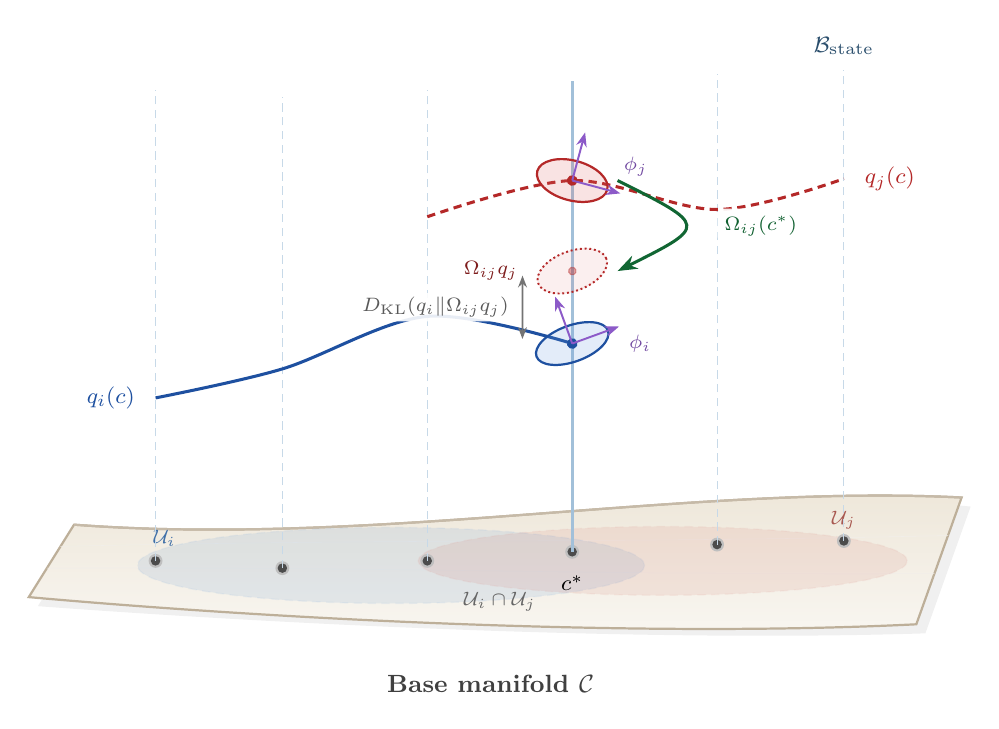
\begin{tikzpicture}[scale=1.15, every node/.style={font=\small}]

% =====================================================================
% COLOR DEFINITIONS
% =====================================================================
\definecolor{fiberblue}{RGB}{70,130,180}
\definecolor{sectionblue}{RGB}{30,80,160}
\definecolor{sectionred}{RGB}{180,40,40}
\definecolor{transportgreen}{RGB}{20,120,60}
\definecolor{gaussblue}{RGB}{100,150,220}
\definecolor{gaussred}{RGB}{220,100,100}
\definecolor{framecol}{RGB}{140,90,200}
\definecolor{basetan}{RGB}{230,220,200}
\definecolor{baseedge}{RGB}{160,140,110}
\definecolor{neighborblue}{RGB}{80,140,210}
\definecolor{neighborred}{RGB}{210,110,100}

% =====================================================================
% BASE MANIFOLD — gently curved surface
% =====================================================================
\path
  (-0.3,0.1) coordinate (M1)
  (9.5,0.4) coordinate (M2)
  (9.0,-1.0) coordinate (M3)
  (-0.8,-0.7) coordinate (M4);

% Shadow
\filldraw[fill=black!6, draw=none]
  ($(M1)+(0.1,-0.1)$)
    .. controls (3.0,-0.2) and (6.5,0.6) .. ($(M2)+(0.1,-0.1)$)
    -- ($(M3)+(0.1,-0.1)$)
    .. controls (6.0,-1.2) and (2.0,-1.0) .. ($(M4)+(0.1,-0.1)$)
    -- cycle;

% Surface fill
\shade[top color=basetan!70, bottom color=basetan!25, draw=baseedge!70, thick]
  (M1)
    .. controls (3.0,-0.15) and (6.5,0.55) .. (M2)
    -- (M3)
    .. controls (6.0,-1.15) and (2.0,-0.95) .. (M4)
    -- cycle;

% Front edge
\draw[baseedge!60, thick]
  (M1) .. controls (3.0,-0.15) and (6.5,0.55) .. (M2);

% Subtle grid lines for depth
\foreach \t in {0.3, 0.6} {
  \draw[baseedge!15, very thin]
    ($(M1)!\t!(M4)$) .. controls
    ($($(M1)!\t!(M4)$)!0.4!($(M2)!\t!(M3)$)+(0,0.04)$) and
    ($($(M1)!\t!(M4)$)!0.6!($(M2)!\t!(M3)$)+(-0.02,-0.04)$)
    .. ($(M2)!\t!(M3)$);
}

\node[below, black!75, font=\small\bfseries] at (4.3,-1.45) {Base manifold $\mathcal{C}$};

% =====================================================================
% FIBER ANCHOR POINTS — six points along the base surface
%
% Layout: C1, C2 in U_i only; C3, C4 in overlap U_i∩U_j;
%         C5, C6 in U_j only.
% =====================================================================
\coordinate (C1) at (0.6,-0.30);
\coordinate (C2) at (2.0,-0.38);
\coordinate (C3) at (3.6,-0.30);
\coordinate (C4) at (5.2,-0.20);
\coordinate (C5) at (6.8,-0.12);
\coordinate (C6) at (8.2,-0.08);

% =====================================================================
% LOCAL OPEN NEIGHBORHOODS U_i, U_j ON THE BASE — with overlap
%
% U_i covers C1–C4 (left through overlap).
% U_j covers C3–C6 (overlap through right).
% Overlap region contains C3, C4 — where both sections coexist.
% =====================================================================

% U_i: agent i's local open set (left to center)
% Center at x=3.0 with x-radius 3.0 → right edge at x=6.0, covering C4 at x=5.2
% y-radius 0.35 keeps the ellipse within the base surface (top edge ~y=0.0 here)
\filldraw[neighborblue, opacity=0.12, draw=neighborblue!60,
          line width=0.5pt, densely dashed]
  (3.2,-0.35) ellipse (2.8 and 0.42);
\node[neighborblue!80!black, font=\scriptsize] at (0.7,-0.05) {$\mathcal{U}_i$};

% U_j: agent j's local open set (center to right)
\filldraw[neighborred, opacity=0.12, draw=neighborred!60,
          line width=0.5pt, densely dashed]
  (6.2,-0.30) ellipse (2.7 and 0.38);
\node[neighborred!80!black, font=\scriptsize] at (8.2,0.15) {$\mathcal{U}_j$};

% Overlap label — between C3 and C4
\node[black!60, font=\scriptsize] at (4.4,-0.75) {$\mathcal{U}_i \cap \mathcal{U}_j$};

% Anchor dots
\foreach \c in {C1,C2,C3,C4,C5,C6} {
  \filldraw[black!25] (\c) circle (2pt);
  \filldraw[black!70] (\c) circle (1.3pt);
}

% =====================================================================
% FIBERS — vertical lines rising from each anchor
% =====================================================================
\pgfmathsetmacro{\fh}{5.2}

\foreach \c in {C1,C2,C3,C4,C5,C6} {
  \draw[fiberblue!30, densely dashed, line width=0.4pt]
    (\c) -- ++(0,\fh);
}

% Fiber label (rightmost)
\node[above=2pt, fiberblue!60!black, font=\footnotesize]
  at ($(C6)+(0,\fh)$) {$\mathcal{B}_{\mathrm{state}}$};

% =====================================================================
% SECTION CURVES — agents i and j as smooth sections of the bundle
%
% CRITICAL: Each section is defined only over its own neighborhood.
%   q_i(c) exists over U_i: fibers C1, C2, C3, C4 (blue section)
%   q_j(c) exists over U_j: fibers C3, C4, C5, C6 (red section)
% Both sections coexist at C3 and C4 (the overlap U_i ∩ U_j).
% =====================================================================

% --- Section q_i (blue, solid) — defined over U_i only (C1–C4) ---
\coordinate (Si1) at ($(C1)+(0,1.8)$);
\coordinate (Si2) at ($(C2)+(0,2.2)$);
\coordinate (Si3) at ($(C3)+(0,2.7)$);
\coordinate (Si4) at ($(C4)+(0,2.3)$);

\draw[sectionblue, line width=1.1pt]
  plot[smooth, tension=0.55] coordinates {
    (Si1) (Si2) (Si3) (Si4)
  };

% --- Section q_j (red, dashed) — defined over U_j only (C3–C6) ---
\coordinate (Sj3) at ($(C3)+(0,3.8)$);
\coordinate (Sj4) at ($(C4)+(0,4.1)$);
\coordinate (Sj5) at ($(C5)+(0,3.7)$);
\coordinate (Sj6) at ($(C6)+(0,4.0)$);

\draw[sectionred, densely dashed, line width=1.1pt]
  plot[smooth, tension=0.55] coordinates {
    (Sj3) (Sj4) (Sj5) (Sj6)
  };

% Section labels — each at the end within its own neighborhood
\node[sectionblue, font=\footnotesize, left=4pt] at (Si1) {$q_i(c)$};
\node[sectionred, font=\footnotesize, right=4pt] at (Sj6) {$q_j(c)$};

% =====================================================================
% HIGHLIGHT FIBER AT c* — at C4, solidly in the overlap U_i ∩ U_j
%
% At this single point c*, BOTH sections q_i(c*) and q_j(c*) live
% in the SAME fiber. The transport Ω_ij(c*) acts WITHIN this fiber
% to align j's frame to i's frame. c* lies in U_i ∩ U_j.
% =====================================================================

% Highlight the fiber at c*
\draw[fiberblue!50, line width=1.0pt] (C4) -- ++(0,\fh);

% Label c* on the base
\node[below=5pt, black, font=\footnotesize\itshape] at (C4) {$c^*$};

% --- Gaussian ellipses at c* showing beliefs in the SAME fiber ---

% q_i(c*): blue Gaussian, frame tilted 20°
\begin{scope}[shift={(Si4)}, rotate=20]
  \filldraw[gaussblue, opacity=0.18] (0,0) ellipse (0.42 and 0.20);
  \draw[sectionblue, line width=0.8pt] (0,0) ellipse (0.42 and 0.20);
  \filldraw[sectionblue] (0,0) circle (1.5pt);
\end{scope}

% q_j(c*): red Gaussian, frame tilted -15° (different gauge frame)
\begin{scope}[shift={(Sj4)}, rotate=-15]
  \filldraw[gaussred, opacity=0.18] (0,0) ellipse (0.40 and 0.22);
  \draw[sectionred, line width=0.8pt] (0,0) ellipse (0.40 and 0.22);
  \filldraw[sectionred] (0,0) circle (1.5pt);
\end{scope}

% --- Local gauge frames at c* (purple axes) ---

% Frame for agent i at c*
\begin{scope}[shift={(Si4)}, rotate=20]
  \draw[-{Stealth[length=1.8mm]}, framecol, line width=0.7pt]
    (0,0) -- (0.55,0);
  \draw[-{Stealth[length=1.8mm]}, framecol, line width=0.7pt]
    (0,0) -- (0,0.55);
\end{scope}
\node[framecol!80!black, font=\scriptsize] at ($(Si4)+(0.75,0.0)$) {$\phi_i$};

% Frame for agent j at c*
\begin{scope}[shift={(Sj4)}, rotate=-15]
  \draw[-{Stealth[length=1.8mm]}, framecol, line width=0.7pt]
    (0,0) -- (0.55,0);
  \draw[-{Stealth[length=1.8mm]}, framecol, line width=0.7pt]
    (0,0) -- (0,0.55);
\end{scope}
\node[framecol!80!black, font=\scriptsize] at ($(Sj4)+(0.7,0.15)$) {$\phi_j$};

% =====================================================================
% GAUGE TRANSPORT Ω_ij — acts WITHIN the fiber over c*
%
% At c*, Ω_ij(c*) rotates q_j(c*) from j's local frame into i's
% local frame. Both distributions live in the same fiber; the
% transport is a frame change, not a spatial translation.
% =====================================================================

% Transported ghost: Ω_ij q_j shown near q_i (now in i's frame, dotted)
% Placed 0.8 above q_i, giving space between q_i and ghost
\coordinate (Ghost) at ($(Si4)+(0,0.8)$);
\begin{scope}[shift={(Ghost)}, rotate=20]
  \filldraw[gaussred, opacity=0.10] (0,0) ellipse (0.40 and 0.22);
  \draw[sectionred, densely dotted, line width=0.7pt] (0,0) ellipse (0.40 and 0.22);
  \filldraw[sectionred, opacity=0.4] (0,0) circle (1.2pt);
\end{scope}

% Ghost label — well to the LEFT to avoid green arrow on the right
\node[sectionred!70!black, font=\scriptsize,
      fill=white, fill opacity=0.9, text opacity=1,
      inner sep=1.5pt, rounded corners=1pt, anchor=east]
  at ($(Ghost)+(-0.55,0)$) {$\Omega_{ij} q_j$};

% Transport arrow: curved arc WITHIN the fiber on the RIGHT side,
% from q_j(c*) down to the ghost near q_i(c*).
% Pushed further right (1.4) to clear the ghost label and ellipse.
\draw[-{Stealth[length=2.5mm, width=1.8mm]},
      transportgreen!85!black, line width=1.1pt]
  ($(Sj4)+(0.5,0)$)
    .. controls ($(Sj4)+(1.5,-0.5)$) and ($(Ghost)+(1.5,0.5)$)
    .. ($(Ghost)+(0.5,0)$);

% Transport label — positioned to the right of the arc, well clear
\node[transportgreen!80!black, font=\scriptsize\bfseries,
      fill=white, fill opacity=0.9, text opacity=1,
      inner sep=2.5pt, rounded corners=2pt, anchor=west]
  at ($(Sj4)!0.5!(Ghost)+(1.6,0)$) {$\Omega_{ij}(c^*)$};

% =====================================================================
% KL DIVERGENCE — between q_i(c*) and transported Ω_ij q_j(c*)
% Both distributions are now expressed in agent i's frame
% within the same fiber over c*. Label on the LEFT side.
% =====================================================================

% Double arrow between q_i and the ghost (left side)
\draw[{Stealth[length=1.5mm]}-{Stealth[length=1.5mm]},
      black!55, line width=0.6pt]
  ($(Si4)+(-0.55,0.05)$) -- ($(Ghost)+(-0.55,-0.05)$);

\node[black!65, font=\scriptsize,
      fill=white, fill opacity=0.9, text opacity=1,
      inner sep=1.5pt, rounded corners=1pt, anchor=east]
  at ($(Si4)+(-0.65,0.40)$) {$D_{\KL}(q_i \| \Omega_{ij} q_j)$};

\end{tikzpicture}
\caption{%
Agent belief sections over the associated bundle
$\mathcal{E}_{\mathrm{state}} = \mathcal{N} \times_{\rho_{\mathrm{state}}} \mathcal{B}_{\mathrm{state}}$.
The shaded surface is the base manifold $\mathcal{C}$;
vertical dashed lines are belief fibers, copies of the statistical manifold
$\mathcal{B}_{\mathrm{state}} = \{\mathcal{N}(\mu, \Sigma) : \mu \in \mathbb{R}^{K_q}, \Sigma \succ 0\}$
over the sample space $\mathbb{R}^{K_q}$.
Agents $i$ and $j$ each have a local open neighborhood on $\mathcal{C}$:
$\mathcal{U}_i$ (blue, dashed) and $\mathcal{U}_j$ (red, dashed).
Each agent's section is defined only over its own neighborhood:
the blue section $q_i(c)$ exists over $\mathcal{U}_i$,
the red section $q_j(c)$ over $\mathcal{U}_j$.
In the overlap $\mathcal{U}_i \cap \mathcal{U}_j$,
both sections coexist in the same fibers.
At the highlighted fiber over $c^* \in \mathcal{U}_i \cap \mathcal{U}_j$,
$q_i(c^*)$ and $q_j(c^*)$ reside in the same fiber
but are expressed in different local gauge frames
$\phi_i$, $\phi_j$ (purple axes).
The transport operator
$\Omega_{ij}(c^*) = \exp(\phi_i)\exp(-\phi_j)$
(green arrow) acts within this fiber,
rotating $q_j$ from $j$'s frame into $i$'s frame
to produce $\Omega_{ij} q_j$ (dotted red ellipse).
The attention cost $D_{\mathrm{KL}}(q_i \| \Omega_{ij} q_j)$
is then the divergence between same-frame distributions within a single fiber.
For transformers ($\dim\mathcal{C} = 0$),
all tokens share one base point, the neighborhoods collapse to a single point,
and the entire computation occurs within one fiber.
}
\label{fig:bundle_sections_surface}
\end{figure}

\subsection{The Base Manifold: Parameter / Index Space of Contexts}

Agents form beliefs about something. We call this underlying domain the base manifold $\mathcal{C}$, following Kant's distinction between phenomena (appearances to observers) and noumena (things-in-themselves). The base manifold represents the parameter / index space of contexts to which agent fields are referred; it plays the structural role of Whitehead's extensive continuum (an abstract framework of relations derived from agentic structure) rather than that of an observer-independent physical substrate. This is consistent with the Section~\ref{sec:lahav_convergence} statement that no observer-independent physical substrate sits underneath the agents: $\mathcal{C}$ is a domain of inquiry, not a thing.

\begin{definition}[Base Manifold]
\label{def:base_manifold}
The base space $\mathcal{C}$ is a smooth $n$-dimensional manifold serving as the parameter / index domain over which agent sections (beliefs, priors, gauge frames, generative models, hyper-priors) are defined.
\end{definition}

\textbf{Conceptual point:} $\mathcal{C}$ is not physical spacetime, and it is not a non-agent physical thing. Within an agent's gauge frame, agent-frame-dependent space-and-time-like structures arise as induced geometries when agents pull back metrics from their belief fields (Section~\ref{sec:pullback}), conditional on the regulator caveats discussed in Section~\ref{sec:consensus_metric}. The base manifold is logically prior to any such induced geometry as the abstract domain of inquiry upon which informational structure is built.

We use local coordinates $c = (c^1, \ldots, c^n)$ on $\mathcal{C}$, though the manifold structure exists independently of coordinate choice.

\subsection{Statistical Manifolds: Beliefs and Models}
\label{sec:statistical_manifolds}

At each point $c \in \mathcal{C}$, agents maintain probability distributions on two information-geometric arenas. The first holds distributions over the latent state $k$ that an agent is trying to infer; the second holds distributions over the parameters $m$ of the agent's generative model. Beliefs and the priors that anchor them live on the first arena, while generative models and their hyper-priors live on the second. These four statistical fields are organized into a fast subsystem $(q_i, p_i)$ that updates on the perceptual timescale and a slow subsystem $(s_i, r_i)$ that updates on the learning timescale, with the priors and hyper-priors interpreted not as independent dynamical variables but as the cross-scale shadows of the beliefs and models at the meta-agent scale immediately above (Section~\ref{sec:participatory}).

\begin{definition}[Statistical Manifolds]
Let
\begin{equation}
\mathcal{B}_{\mathrm{state}} = \{\mathcal{N}(\mu, \Sigma) : \mu \in \mathbb{R}^{K_q}, \Sigma \succ 0\},
\qquad
\mathcal{B}_{\mathrm{model}} = \{\mathcal{N}(\mu, \Sigma) : \mu \in \mathbb{R}^{K_m}, \Sigma \succ 0\}
\end{equation}
denote the finite-dimensional manifolds of Gaussian distributions over the latent state $k \in \mathbb{R}^{K_q}$ and over the generative-model parameters $m \in \mathbb{R}^{K_m}$, respectively. Each is equipped with the Fisher-Rao metric, given in the coordinates $\theta = (\mu, \Sigma)$ by
\begin{equation}
g_{\mathcal{B}}(\partial_a, \partial_b) = \mathbb{E}\left[(\partial_a \log \rho_\theta)(\partial_b \log \rho_\theta)\right],
\end{equation}
with $\rho_\theta$ the corresponding Gaussian density and indices $a, b$ ranging over the coordinates $(\mu, \Sigma)$.
\end{definition}

The same coordinate formula extends formally to any smooth finite-dimensional parametric family with suitably integrable score; a rigorous extension to the full nonparametric space of distributions requires additional structure that we do not need, since the fibers $\mathcal{B}_{\mathrm{state}}$ and $\mathcal{B}_{\mathrm{model}}$ are populated exclusively by Gaussian families and the Fisher-Rao metric is evaluated only on them in this manuscript. The Gaussian form of the two fibers is the manuscript-wide working realization rather than a structural necessity: Section~\ref{sec:working_framework} lists it among the practical simplifications, the construction applies to any exponential-family fiber, and the pan-agentic ontology of Section~\ref{sec:cognitive_first} contemplates non-Gaussian and density-operator fibers. Non-Gaussian objects do appear elsewhere as auxiliary constructions, in particular the finite Gaussian mixtures of the mixture-of-sources energy (Eq.~\eqref{eq:mixture_joint}) and of the moment-matched coarse-graining covariance (Section~\ref{sec:meta_agent_state_construction}), and the categorical attention distributions $\beta(z)$; none of these carries the fibers' Fisher-Rao structure.

Beliefs $q_i$ and priors $p_i$ both take values in $\mathcal{B}_{\mathrm{state}}$, while generative models $s_i$ and hyper-priors $r_i$ both take values in $\mathcal{B}_{\mathrm{model}}$. The two manifolds are generically distinct because the latent state $k$ and the model parameters $m$ are different objects with different sample spaces, and may have different dimensions.

The Fisher-Rao metric provides natural Riemannian geometry on probability spaces. It measures how distinguishable nearby distributions are statistically: distributions with sharper peaks (higher information content) are further apart. The metric is unique up to scaling as the only Riemannian metric on probability spaces invariant under sufficient statistics; Chentsov's original theorem~\cite{Cencov1982} covers finite sample spaces, and the continuous-parametric extension relevant to the Gaussian families used here is supplied by Ay, Jost, L\^{e}, and Schwachh\"{o}fer~\cite{AyJostLeSchwachhofer2017}.

As defined above, the two arenas are the spaces of $K_q$- and $K_m$-dimensional multivariate Gaussian distributions, parametrized by mean vectors and positive-definite covariance matrices and forming $(K_q + K_q(K_q+1)/2)$- and $(K_m + K_m(K_m+1)/2)$-dimensional manifolds respectively.

The Fisher-Rao metric naturally induces several information-theoretic quantities. The Kullback-Leibler divergence between two distributions $q$ and $p$ on the same manifold measures their relative entropy

\begin{equation}
\mathrm{KL}(q \| p) = \int q(x) \log\frac{q(x)}{p(x)} dx \geq 0.
\end{equation}

This divergence is not symmetric ($\mathrm{KL}(q \| p) \neq \mathrm{KL}(p \| q)$) but it generates the Fisher metric through its Hessian structure. The natural gradient $\tilde{\nabla}_q f = g^{-1}_{\mathcal{B}} \nabla_q f$ provides the steepest descent direction in the curved probability space.

For Gaussian distributions specifically, the KL divergence has closed form:
\begin{equation}
\mathrm{KL}(\mathcal{N}(\mu_1, \Sigma_1) \| \mathcal{N}(\mu_2, \Sigma_2)) = \frac{1}{2}\left[\log\frac{|\Sigma_2|}{|\Sigma_1|} + \mathrm{tr}(\Sigma_2^{-1}\Sigma_1) + (\mu_2 - \mu_1)^\top\Sigma_2^{-1}(\mu_2 - \mu_1) - K_q\right]
\label{eq:gaussian_kl}
\end{equation}

This formula will be used extensively for computing belief and prior alignment terms; the associated Fisher information matrix on the Gaussian fiber, the matrix exponential identities for $\mathrm{SO}(3)$ transport, and the Cholesky parameterization of positive-definite covariances used in the numerical implementation are collected, as stated results, in Appendix~\ref{app:math}, and the gradient-flow analysis of the resulting covariance fixed-point equation is in Appendix~\ref{app:covariance_dynamics}.

\subsection{Cross-Scale Shadows: Priors and Hyper-priors as Cross-Scale Constructs}
\label{sec:cross_scale_shadows}

A central economy of the framework is that the prior $p_i^{(s)}$ and the hyper-prior $r_i^{(s)}$ at scale $s$ are not independent dynamical fields but are determined by top-down transport from the meta-agent that envelopes agent $i$ at scale $s+1$. Concretely,
\begin{equation}
p_i^{(s)}(c) = \Omega_{i,I}\big[q_I^{(s+1)}\big](c),
\qquad
r_i^{(s)}(c) = \tilde\Omega_{i,I}\big[s_I^{(s+1)}\big](c),
\label{eq:cross_scale_shadow}
\end{equation}
where $I$ indexes the meta-agent at scale $s+1$ that contains agent $i$ as a constituent, $\Omega_{i,I}$ is the gauge-covariant transport into agent $i$'s frame on the latent-state fiber, and $\tilde\Omega_{i,I}$ is its model-fiber counterpart. The fast-channel relation is the formal content of the participatory feedback equation at Eq.~\eqref{eq:topdown_priors}; the slow-channel relation is its model-channel mirror. Because the prior $p_i^{(s)}$ is defined as the gauge transport of the meta-agent's posterior $q_I^{(s+1)}$, beliefs and priors share the latent-state manifold $\mathcal{B}_{\mathrm{state}}$ by construction, and the same definitional move places $r$ and $s$ on the same manifold $\mathcal{B}_{\mathrm{model}}$. This is a structural commitment of the framework rather than a theorem of standard hierarchical variational inference: in the standard scheme~\cite{Friston2017, parr2022active} the level-$\ell$ prior is derived from a generative-model conditional $p(s_\ell \mid s_{\ell+1})$, not posited as a transported posterior. The framework realizes the transported-posterior identification as the rigid-link specialization of an augmented hierarchical generative model carried out explicitly in Appendix~\ref{app:augmented_joint}: a joint with Gibbs cross-scale factors $\chi_{i,\pi(i)}(k_i, k_{\pi(i)}) \propto \exp[-\|k_i - \Omega_{i,\pi(i)}k_{\pi(i)}\|^2/(2\sigma^2)]$ (appendix notation: $\pi(i)$ is the parent map written $\mathrm{pa}(i)$ in the body) defines a well-defined probability density on the product space of all agent-scale latents (Lemma~\ref{lem:aug_joint_welldefined}), and the cross-scale shadow $p_i^{(s)} = \Omega_{i,I}[q_I^{(s+1)}]$ is the $\sigma^2 \to 0$ limit of the parent-predictive prior, the marginal of the cross-scale Gibbs factor against the parent's variational posterior (Lemma~\ref{lem:shadow_mf_optimum}); this predictive prior coincides with the marginal of the joint itself only insofar as the variational parent matches the exact parent marginal. The standard scheme's conditional density $p(s_\ell \mid s_{\ell+1})$ corresponds to the finite-$\sigma^2$ Gibbs factor of Eq.~\eqref{eq:gibbs_factor}; the present manuscript takes the rigid-link $\sigma^2 \to 0$ specialization as a structural commitment of the framework rather than as a derivation from any peer-reviewed hierarchical-VI precedent. The continuity with~\cite{Friston2010, Friston2017, parr2022active} is at the variational-principle backbone (ELBO, complexity/accuracy decomposition, natural-gradient flow) and at the augmented-joint generative-model structure of Appendix~\ref{app:augmented_joint}; the rigid-link identification is the framework's own specialization within that structure and is not inherited from~\cite{Friston2017, parr2022active}. Conditional on Eq.~\eqref{eq:cross_scale_shadow}, the hierarchy $r \to s \to p \to q \to \text{observations}$ posited at the agent definition below is realized cross-scale: $r$ regularizes $s$ because $r$ is the meta-agent's model transported down, and $p$ regularizes $q$ because $p$ is the meta-agent's belief transported down.

The hierarchy bottoms out at two boundaries. At the top scale ($s = s_{\max}$) there is no enveloping meta-agent, so the hyper-prior $r_i^{(s_{\max})}$ is treated as a fixed boundary condition encoding evolutionary or training-time structural defaults, and the top-scale prior is set self-referentially by aggregating across all active agents (Section~\ref{sec:participatory}). At the bottom scale ($s = 0$) the system has no constituents below it, so cross-scale propagation acts only downward from above. In the empirical simulations of Section~\ref{sec:meta_agent_emergence} all agents reside at a single scale and $p_i, r_i$ are treated as primitive boundary conditions with no super-agent above; the multi-scale relation~\eqref{eq:cross_scale_shadow} becomes operative only in the participatory dynamics of Section~\ref{sec:participatory}.

\subsection{Principal Bundles and Gauge Freedom}
\label{sec:agents_as_sections}

We now address the third challenge: different agents use different internal (cognitive) reference frames when representing beliefs and models. A physicist measuring particle spin uses basis vectors in their laboratory frame. Another physicist with a rotated laboratory measures the same physics but obtains different numerical values. Both descriptions are equally valid - they're related by transformations.

More generally, agents maintain beliefs using internal coordinate systems, conceptual frameworks, or measurement conventions: their gauge frames. These frames are necessary for representing probabilistic information, and the framework employs them in two distinct roles that the reader must keep separate.

\paragraph{Two roles for the gauge frame.} The same symbol $\phi_i$ does double duty in this manuscript, and conflating the two roles is the source of several apparent contradictions. In its \emph{transport role} (Role A), the frame is gauge-redundant: any pair of frame fields $\phi_i, \phi_j$ enters the dynamics only through the relative transport $\Omega_{ij} = U_iU_j^{-1}$, which is invariant under simultaneous right-translation $U_i \mapsto U_i g$ for all agents (Section~\ref{sec:transport}). Observable consequences of the transport structure depend only on the orbit of the frame collection under this global gauge action; an isolated frame carries no physical content. This is the redundancy reading the manuscript invokes when it speaks of "arbitrary frames" or "gauge invariance" of observables. In its \emph{state role} (Role B), the per-agent frame is treated as an internal cognitive state variable that contributes to ontology: distinct agent frames generate distinct frame-dependent pulled-back geometries $G_i^{(q)}$ (Section~\ref{sec:pullback}), distinct phenomenal characters in the qualia discussion (Section~\ref{sec:qualia}), and distinct signature mechanisms in the worked example of Section~\ref{sec:signature_resolution}. Quantities computed in Role B (such as $G_i^{(q)}$ or $\mathrm{tr}(A^{(i)}_\mu A^{(i)}_\nu)$) are frame-dependent: they are invariant under the constant-per-agent residual subgroup ($U_i \mapsto U_i g$ with $g$ constant in $c$, by trace cyclicity) but not under the full local gauge $g_i = g_i(c)$, which introduces a Maurer-Cartan term. They depend on the Role-B cognitive state $\phi_i$ rather than being redundant labels, which is the sense in which they carry ontology (see the residual-subgroup analysis below). The framework makes both roles available without identifying the frame in Role B with mere description; any sentence that calls the frame "pure gauge" or "arbitrary" is invoking Role A, while any sentence in which the frame contributes to phenomenology, signature, or ontology is invoking Role B. Gauge-invariant observables of the framework are recovered from Role-B quantities by averaging over the gauge orbit (Section~\ref{sec:consensus_metric}); when no such average is taken, what is computed is a frame-dependent quantity, and we say so.

In what follows, the words "gauge-invariant" and "gauge-covariant" are reserved for their standard mathematical meanings: invariant means unchanged under the simultaneous right-translation, covariant means transforming according to a fixed representation. We use "frame-dependent" rather than "gauge-dependent" when referring to Role-B quantities, to signal that the dependence is on the cognitive state $\phi_i$ rather than on a redundant labeling.

\paragraph{Precedents and residual-subgroup structure of the dual role.}
\label{sec:dual_role_rigor}
The simultaneous Role-A / Role-B treatment of $\phi_i$ is motivated by three well-developed mechanisms in modern gauge theory and quantum reference frames, cited here as precedents rather than as constructions reproduced in this framework. Edge modes in gauge theory~\cite{DonnellyFreidel2016} promote "would-be pure-gauge" boundary data to genuine physical degrees of freedom whenever a region's interior is treated as a subsystem: the boundary modes are gauge-redundant from the global standpoint but carry physical, symplectically conjugate information at the boundary of the subsystem. Quantum reference frames~\cite{BartlettRudolphSpekkens2007, Vanrietvelde2020, giacomini2019qrf} formalize this for finite quantum systems: a reference frame is gauge from a global perspective-neutral viewpoint, but is a physical system carrying state from its own perspective and from that of any other system relative to which it is described. The two readings attach to different subgroups, which is what licenses the dual role rather than making it inconsistent: the perspective-neutral construction of Vanrietvelde et al.~\cite{Vanrietvelde2020} is the cleanest precedent for the global-diagonal redundancy (Role~A), while the genuine frame-relativity of entanglement established by Giacomini et al.~\cite{giacomini2019qrf} supports the residual, frame-carried content (Role~B). Rovelli's relational interpretation~\cite{Rovelli1996}, already cited as the closest physics-side antecedent, is consistent with both readings and so does not by itself decide which subgroup is physical; it sits in the same family: properties have meaning only relative to other systems, and "the same data" is gauge or physical depending on which slice of the relational structure one inspects. Each of these literatures argues, by independent routes, that a frame field can serve both roles when one is precise about which gauge subgroup is acting. We do not construct the corresponding structures here: there is no boundary symplectic form, no conjugate charges, and no theorem forcing the Role-B frame data from a subsystem decomposition, so the parallel is motivation rather than proof. What the framework does deliver is consistency: a precise statement of which subgroup acts on which quantity, given in the next paragraph as the bulk global-diagonal action versus the constant-per-agent residual subgroup, together with the trace-cyclicity invariance under the latter.

In the present framework, the bulk gauge action is the global diagonal right-translation $U_i \to U_i g$ for a single $g \in G$ shared across all agents; under this action $\phi_i$ is purely redundant and only $\Omega_{ij}$ is invariant, in agreement with Role~A. The agent-local frame data $\phi_i: \mathcal{U}_i \to \mathfrak{g}$ is the analog of edge-mode / quantum-reference-frame content: from the perspective of the network the choice of $\phi_i$ at a single agent specifies that agent's relational stance and is physical, in agreement with Role~B. Quantities like $\mathrm{tr}(A^{(i)}_\mu A^{(i)}_\nu)$ are not invariant under the full local gauge $g_i = g_i(c)$ that introduces a Maurer-Cartan derivative term, but are invariant under the constant-per-agent residual subgroup $\{(g_i)_{i \in I} : g_i \in G \text{ constant in } c\}$, since $\mathrm{tr}(g^{-1}A_\mu g \cdot g^{-1}A_\nu g) = \mathrm{tr}(A_\mu A_\nu)$ by trace cyclicity when $g$ is $c$-constant. The Lorentzian-signature mechanism, the pulled-back metric, and the gauge-curvature linguistic conjecture therefore live under this residual subgroup rather than under the full local gauge; we attach this restriction to each occurrence below rather than appealing to a uniformly stated invariance.

\begin{definition}[Principal Bundle]
Let $\pi: \mathcal{N} \to \mathcal{C}$ be a principal $G$-bundle where:
\begin{itemize}
\item $\mathcal{N}$ is the total space (all possible gauge choices at all base points)
\item $\mathcal{C}$ is the base manifold (the noumenal domain)
\item $G$ is the structure group, acting freely on the right on $\mathcal{N}$
\end{itemize}
The projection satisfies $\pi(n \cdot g) = \pi(n)$ for all $g \in G$, so the group action preserves fibers; $G$ acts freely and transitively on each fiber $\pi^{-1}(c)$, so that $\mathcal{N}/G \cong \mathcal{C}$; and the bundle is locally trivial, $\mathcal{N}|_{\mathcal{U}} \cong \mathcal{U} \times G$ as $G$-spaces for sufficiently small open $\mathcal{U} \subseteq \mathcal{C}$.
\end{definition}

In this manuscript the structure group is typically the compact $G = \mathrm{SO}(N)$ in the proof-of-concept simulations, while the natural group for KL-based variational inference on Gaussian fibers is the real $\mathrm{GL}(K_q, \mathbb{R})$; the distinction is drawn at the end of this subsection and developed in Section~\ref{sec:gauge_group_choice}.

\paragraph{Local trivializations and the scope of the bundle formalism.}
\label{sec:local_trivialization}
A general principal $G$-bundle does not admit a global section: a globally defined Lie-algebra-valued frame field $\phi: \mathcal{C} \to \mathfrak{g}$ exists if and only if the bundle is trivializable, i.e., $\mathcal{N} \cong \mathcal{C} \times G$ as a $G$-space. The framework as constructed below operates in local trivializing patches $\{\mathcal{U}_i\}$ that cover $\mathcal{C}$, with each $\phi_i: \mathcal{U}_i \to \mathfrak{g}$ a local section of the trivialization restricted to agent~$i$'s domain of operation. On overlaps $\mathcal{U}_i \cap \mathcal{U}_j$, the operator $\Omega_{ij} = U_iU_j^{-1}$ is the transition function between the trivializations induced by $U_i$ and $U_j$, and satisfies the standard \v{C}ech cocycle condition $\Omega_{ij}\Omega_{jk} = \Omega_{ik}$ on triple overlaps (Lemma~\ref{thm:vanishing_holonomy}). Because each $U_i$ is defined on the whole of its patch, this \v{C}ech data is by construction the coboundary of the family $\{U_i\}$, so the bundle it reconstructs is canonically trivializable; we accordingly assume a fixed reference trivialization throughout, realized in the implementation as the shared ambient frame (cf. the data-dependent-connection discussion in Section~\ref{sec:discrete_regime_ii}), and the bundle language is organizational rather than a source of topological generality. Transition data that is not a coboundary (nontrivial bundle topology) is out of scope of the present construction, consistent with the global-topology concessions of Section~\ref{sec:working_framework}. We also distinguish the two roles $\Omega_{ij}$ plays: in the dynamics the agent beliefs $q_i$ are \emph{distinct} sections compared within a common frame, with $\mathrm{KL}(q_i \| \Omega_{ij} q_j) > 0$ generically, so $\Omega_{ij}$ enters as a transport operator between agents rather than as a gluing map identifying local representatives of one section. The framework's nontrivial-holonomy extension (Section~\ref{sec:discrete_regime_ii}) is the lattice gauge promotion of the cocycle in which the link variables (transport operators) acquire an independent edge-local connection $\delta_{ij}$ between vertex factors.

Two technical caveats accompany this restriction. First, the exponential parameterization $U_i(c) = \exp[\phi_i(c)]$ is only locally bijective: the exponential map $\exp: \mathfrak{g} \to G$ is surjective for connected compact groups (such as the $G = \mathrm{SO}(N)$ used in the proof-of-concept simulations), but for the non-compact group $\mathrm{GL}^+(K_q)$ relevant to the natural variational-inference setting, a single $\phi$ does not parameterize every group element. This is handled either by restricting $\phi_i$ to a neighborhood of zero on which $\exp$ is bijective, or by passing to a polar/Cartan decomposition $U = \exp(X)\exp(Y)$ with two Lie-algebra elements (one symmetric, one antisymmetric) so that the full group is covered by two exponential charts; the emergence simulation uses the compact $\mathrm{SO}(3)$ representation, where the issue does not arise; the reference implementation and the WikiText-103 sweep operate in noncompact $\mathrm{GL}^+(K_q)$, where this caveat applies. Second, the Maurer-Cartan one-form $\theta = U^{-1}dU$ in Section~\ref{sec:connection_forms} below is well-defined on each local patch independently of whether the global bundle is trivializable; the patch-wise cocycle structure is what the framework actually requires, and references to "the global frame field $\phi$" in subsequent discussion should be read in the local-trivialization sense unless explicitly noted otherwise.

Intuitively, each point $c \in \mathcal{C}$ sits above a fiber $\pi^{-1}(c) \cong G$ consisting of all possible gauge choices at that location. Moving within a fiber corresponds to changing reference frame without changing which point of $\mathcal{C}$ we're considering. The group $G$ parametrizes these frame transformations - for $G = \mathrm{SO}(3)$, these are rotations of internal coordinate axes.

This abstraction captures gauge freedom in physics (electromagnetic gauge transformations, coordinate changes in general relativity) but applies more broadly to any setting where agents must choose conventions for representing information. A cognitive agent's gauge frame might encode perceptual reference axes, categorical schemes, or other aspects of subjective framing.

The natural gauge group for KL-based variational inference on multivariate Gaussians is the real $G = \mathrm{GL}(K_q, \mathbb{R})$ acting on the belief fiber, with the proof-of-concept simulations in this work restricted to the compact subgroup $G = \mathrm{SO}(3)$ for computational tractability and visualizability. A separate complex $\mathrm{GL}(K_q, \mathbb{C})$ acts on the gauge connection only and is invoked in the worked Lorentzian-signature example of Section~\ref{sec:signature_resolution}; it does not act on the belief fiber. The full justification of this choice, including the formal $\mathrm{GL}(K_q, \mathbb{R})$ invariance theorem and the connection-only role of the complex extension, is given in Section~\ref{sec:gauge_group_choice}.

\subsection{Associated Bundles: Attaching Probability Distributions to Gauge Structure}

Having established gauge structure through the principal bundle, we attach the two statistical manifolds $\mathcal{B}_{\mathrm{state}}$ and $\mathcal{B}_{\mathrm{model}}$ in a way that respects gauge transformations. This is accomplished through associated bundles, a standard construction in differential geometry~\cite{nakahara2003geometry, frankel2011geometry}.

The construction is as follows: if we change gauge frame (move within a fiber of $\mathcal{N}$), the probability distributions must transform accordingly. This requires specifying how the gauge group $G$ acts on each statistical manifold.

\begin{definition}[Representations and Associated Bundles]
Let $\rho_{\mathrm{state}}: G \to \mathrm{Aut}(\mathcal{B}_{\mathrm{state}})$ and $\rho_{\mathrm{model}}: G \to \mathrm{Aut}(\mathcal{B}_{\mathrm{model}})$ be smooth representations of $G$ on the two statistical manifolds. The associated bundles are
\begin{align}
\mathcal{E}_{\mathrm{state}} &:= \mathcal{N} \times_{\rho_{\mathrm{state}}} \mathcal{B}_{\mathrm{state}} \\
\mathcal{E}_{\mathrm{model}} &:= \mathcal{N} \times_{\rho_{\mathrm{model}}} \mathcal{B}_{\mathrm{model}}
\end{align}
where the equivalence relation $(n \cdot g, b) \sim (n, \rho(g)b)$ identifies gauge-transformed pairs and the appropriate $\rho$ is determined by which manifold $b$ inhabits.
\end{definition}

\paragraph{Convention.} The equivalence relation $(n\cdot g, b) \sim (n, \rho(g)b)$ adopted above corresponds to treating $\rho: G \to \mathrm{Aut}(\mathcal{B})$ as a left action paired with the right principal action $n \mapsto n\cdot g$ on $\mathcal{N}$; this is the convention used in~\cite{nakahara2003geometry}. It is mathematically equivalent (under $g \mapsto g^{-1}$ and the homomorphism property $\rho(g^{-1}) = \rho(g)^{-1}$) to the alternative convention $(n\cdot g, b) \sim (n, \rho(g^{-1})b)$ found in some texts, in which $\rho$ is treated as the right action induced from the left action. Throughout this manuscript we use the $(n\cdot g, b) \sim (n, \rho(g)b)$ form consistently; transport laws, gauge-covariance arguments, and the lattice gauge transformation $\Omega_{ij} \mapsto g_i \Omega_{ij} g_j^{-1}$ in Section~\ref{sec:transport} are stated relative to this convention, with the per-vertex $g_i \in G$ restricted to the constant-per-agent residual subgroup of Section~\ref{sec:dual_role_rigor} for Role-B quantities that are not invariant under the full local gauge. A reader importing identities from a text with the inverse convention should substitute $\rho(g) \to \rho(g^{-1})$ everywhere.

For Gaussian distributions with $G = \mathrm{GL}(K_q)$ (or any subgroup such as $\mathrm{SO}(N)$), the representation acts by linear transformation of means and congruence of covariances:
\begin{equation}
\rho_{\mathrm{state}}(g) \cdot \mathcal{N}(\mu, \Sigma) = \mathcal{N}(g\mu, g\Sigma g^\top),
\end{equation}
and analogously for $\rho_{\mathrm{model}}$ acting on the model-parameter fiber. The qualifier "analogously" requires specification when the fiber dimensions differ: for the congruence form to be type-correct on the $K_m$-dimensional model fiber, $\rho_{\mathrm{model}}$ must be realized as an $K_m$-dimensional representation of $G$, and no canonical choice exists for generic $K_m \neq K_q$. We therefore fix it explicitly. For the compact case $G = \mathrm{SO}(3)$, $\rho_{\mathrm{model}}$ is assembled as a direct sum of irreducible representations of total dimension $K_m$, the same device used for high-dimensional belief fibers in Section~\ref{sec:gauge_group_choice}; for $G = \mathrm{GL}(K_q)$ we take $K_m = K_q$ with the fundamental representation. Alternatively, the framework admits giving the model fiber its own principal bundle with structure group $\mathrm{GL}(K_m)$ and an independent frame field $\tilde{\phi}_i$, so that $\tilde{\Omega}_{ij} = \exp(\tilde{\phi}_i)\exp(-\tilde{\phi}_j)$ is a transport in its own right rather than the image of $\Omega_{ij}$ under a representation; this is the configuration realized by the reference implementation and the independent-frame option of the envelope-gradient discussion following Eq.~\eqref{eq:envelope_gradient_model}. Either choice ensures that changing reference frame transforms probability distributions consistently. When $g \in \mathrm{SO}(N)$, this reduces to rotation; for general $g \in \mathrm{GL}(K_q)$, it includes scaling, shearing, and reflection. The associated bundles $\mathcal{E}_{\mathrm{state}}$ and $\mathcal{E}_{\mathrm{model}}$ are fiber bundles over $\mathcal{C}$ with fibers isomorphic to $\mathcal{B}_{\mathrm{state}}$ and $\mathcal{B}_{\mathrm{model}}$ respectively, and the four agent fields $(q_i, p_i)$ and $(s_i, r_i)$ are sections of these two bundles, with the prior and hyper-prior derived from the meta-scale via Eq.~\eqref{eq:cross_scale_shadow}.

\subsection{Agents as Smooth Sections}
\label{sec:agent_definition}

We can now define agents precisely as sections of these associated bundles, smooth by hypothesis at the primitive scale. For the emergent meta-agents of higher scales, whose fields are constructed by coarse-graining rather than posited, the regularity available is correspondingly weaker: smooth on the interior of the formation support under the smooth-bump convention of Section~\ref{sec:complete_free_energy}, and only measurable, piecewise-smooth across support boundaries (see the Meta-Agent definition below).

\begin{definition}[Agent]
An agent $\mathcal{A}^i$ at scale $s$ with support domain $\mathcal{U}_i \subseteq \mathcal{C}$ consists of two primitive smooth sections together with two derived sections and a gauge-frame field:
\begin{align}
q_i &: \mathcal{U}_i \to \mathcal{E}_{\mathrm{state}}|_{\mathcal{U}_i}, &&\text{(belief, primitive)} \\
s_i &: \mathcal{U}_i \to \mathcal{E}_{\mathrm{model}}|_{\mathcal{U}_i}, &&\text{(generative model, primitive)} \\
p_i &= \Omega_{i,I}\big[q_I^{(s+1)}\big] \in \Gamma\left(\mathcal{E}_{\mathrm{state}}|_{\mathcal{U}_i}\right), &&\text{(prior, derived)} \\
r_i &= \tilde\Omega_{i,I}\big[s_I^{(s+1)}\big] \in \Gamma\left(\mathcal{E}_{\mathrm{model}}|_{\mathcal{U}_i}\right), &&\text{(hyper-prior, derived)} \\
\phi_i &: \mathcal{U}_i \to \mathfrak{g}, &&\text{(gauge frame field)}
\end{align}
where $\mathfrak{g} = \mathrm{Lie}(G)$ is the Lie algebra of the gauge group and $I = \mathrm{pa}(i)$ indexes the level-$(s{+}1)$ meta-agent, if any, that envelopes agent $i$ as a constituent (the parent map is written $\pi(i)$ in Appendix~\ref{app:augmented_joint}; we write $\mathrm{pa}(i)$ in the body to avoid collision with the bundle projection $\pi: \mathcal{N} \to \mathcal{C}$). The derived sections are defined conditionally on such a parent existing: meta-agents form only when the threshold criteria of the Meta-Agent definition below are met, and we import the hypotheses of the appendices, under which the parent assignment is a map $\mathrm{pa}(i)$ on a finite tree (Appendix~\ref{app:augmented_joint}) induced by a measurable partition $\mathcal{P}_s$ of each scale (Appendix~\ref{app:rigorous_rg}). These hypotheses are idealizations that the reported simulation does not satisfy: the run of Section~\ref{sec:meta_agent_emergence} produces a time-accumulated hierarchy of condensation events whose per-scale populations form neither a partition of the scale below nor a single tree on the base agents, as disclosed there. The transported parent fields define $p_i$ and $r_i$ on $\mathcal{U}_i \cap \mathcal{U}_I$; where agent $i$ operates without a parent, either because no cluster containing $i$ meets the formation criteria or on the portion of $\mathcal{U}_i$ outside the parent's support, the prior and hyper-prior revert to primitive boundary conditions, fixed or learned, as in the single-scale simulations (Section~\ref{sec:cross_scale_shadows}) and the transformer limit (Section~\ref{sec:transformers}). The four statistical sections are organized as the variational hierarchy
\[
r_i \to s_i \to p_i \to q_i \to \text{observations},
\]
realized cross-scale via Eq.~\eqref{eq:cross_scale_shadow}: $r_i^{(s)}$ regularizes $s_i^{(s)}$ because $r_i^{(s)}$ is the meta-agent's generative model transported down, and $p_i^{(s)}$ regularizes $q_i^{(s)}$ because $p_i^{(s)}$ is the meta-agent's belief transported down. At the top scale, $r_i^{(s_{\max})}$ becomes a fixed boundary condition encoding evolutionary or training-time defaults; at the bottom scale, the cross-scale relations act only downward. In the empirical simulations of this paper the slow subsystem $(s_i, r_i)$ is held fixed (model coupling $\gamma_{ij} = 0$) and only the fast subsystem $(q_i, p_i)$ is updated, with $p_i$ realized concretely by the per-token PriorBank (Section~\ref{sec:transformers}). The slow subsystem is retained in the free energy because it is required for the meta-agent / Ouroboros dynamics of Section~\ref{sec:participatory}, where consensus on generative models is the conceptual content of the $\gamma_{ij}\mathrm{KL}(s_i\|\tilde{\Omega}_{ij}s_j)$ term.
\end{definition}

The notation requires unpacking. Each agent maintains smooth probability distributions $q_i(c)$ and $p_i(c)$ at every point $c$ in their domain of operation $\mathcal{U}_i$. These are not single distributions but entire fields - functions mapping base manifold points to probability distributions. The gauge frame $\phi_i(c) \in \mathfrak{g}$ specifies which reference frame the agent uses at location $c$, encoded as a Lie algebra element generating local gauge transformations.

For Gaussian agents, this specializes to:
\begin{align}
q_i(c) &= \mathcal{N}(\mu_i(c), \Sigma_i(c)) \\
p_i(c) &= \mathcal{N}(\mu_i^p(c), \Sigma_i^p(c)) \\
s_i(c) &= \mathcal{N}(\mu_i^s(c), \Sigma_i^s(c)) \\
r_i(c) &= \mathcal{N}(\mu_i^r(c), \Sigma_i^r(c)) \\
\phi_i(c) &= \phi_i^a(c) G_a
\end{align}

where $\mu_i, \mu_i^p: \mathcal{U}_i \to \mathbb{R}^{K_q}$ are means on the latent-state fiber $\mathcal{B}_{\mathrm{state}}$ with $\Sigma_i, \Sigma_i^p \in \mathbb{S}^{K_q}_{++}$, while $\mu_i^s, \mu_i^r: \mathcal{U}_i \to \mathbb{R}^{K_m}$ are means on the model-parameter fiber $\mathcal{B}_{\mathrm{model}}$ with $\Sigma_i^s, \Sigma_i^r \in \mathbb{S}^{K_m}_{++}$. The pair $(\mu_i^p, \Sigma_i^p)$ is determined by Eq.~\eqref{eq:cross_scale_shadow} from the level-$(s{+}1)$ meta-agent's belief, and $(\mu_i^r, \Sigma_i^r)$ analogously from the meta-agent's generative model. The fields $\phi_i^a(c)$ are scalar coefficients, and $\{G_a\}$ are basis generators of the Lie algebra $\mathfrak{g}$ (specialized to $\mathfrak{so}(N)$ in the proof-of-concept simulations).

This formulation provides complete flexibility. Agents can maintain different beliefs at different locations (spatial variation in $q_i(c)$). They can use different reference frames at different locations (spatially varying gauge $\phi_i(c)$). Multiple agents can overlap spatially, each maintaining their own beliefs about the same region of $\mathcal{C}$. This generality will prove essential for modeling everything from transformer attention mechanisms to multi-agent coordination to emergent spacetime structure.

The framework is now mathematically complete: we have base manifold, statistical fibers, gauge structure, and agents as sections. The next step is introducing dynamics through variational free energy minimization.

\subsection{Multi-Agent Systems and Overlapping Perspectives}

\subsubsection{The Multi-Agent Configuration}

Effective shared structure in this framework arises not from a single observer but from collective dynamics of multiple agents maintaining overlapping beliefs about the same underlying noumenal substrate. This multiplicity is essential within the framework: a single agent alone cannot generate the intersubjective structure that the construction takes as a formal correlate of objective reality.

\begin{definition}[Multi-Agent System]
A multi-agent system $\mathcal{M}$ over base manifold $\mathcal{C}$ consists of a finite collection of agents:
\begin{equation}
\mathcal{M} = \left\{\mathcal{A}^i = (q_i, p_i, s_i, r_i, \phi_i)\right\}_{i \in \mathcal{I}},
\end{equation}
where $\mathcal{I}$ is an index set (typically $\mathcal{I} = \{1, 2, \ldots, N\}$), and each agent $\mathcal{A}^i$ operates over domain $\mathcal{U}_i \subseteq \mathcal{C}$. When the slow subsystem is held fixed, as in the simulations below, an agent is referred to by the abbreviated tuple $(q_i, p_i, \phi_i)$ without ambiguity.
\end{definition}

The domains $\mathcal{U}_i$ generally overlap, with $\mathcal{U}_i \cap \mathcal{U}_j \neq \emptyset$ for many agent pairs. This overlap is not incidental but fundamental - agents must share common ground to exchange information and coordinate beliefs. The intersection $\mathcal{U}_i \cap \mathcal{U}_j$ represents the region where both agents maintain explicit beliefs, enabling comparison and information exchange despite their potentially different gauge frames.

Each agent represents an autonomous information-processing entity with its own beliefs, priors, and reference frame. The domain $\mathcal{U}_i$ delineates the region of $\mathcal{C}$ about which agent $i$ maintains representations. In physical contexts, this might correspond to sensory range - a human observer can only form beliefs about the spatial region accessible to their senses. In cognitive contexts, different brain modules might process overlapping aspects of sensory input, each maintaining beliefs over partially overlapping representational spaces. In social contexts, communities maintain beliefs over shared cultural knowledge, with overlaps representing common ground for communication. In linguistic contexts, speakers maintain beliefs over semantic space, with overlaps representing shared meanings enabling successful communication.

\subsubsection{Consensus and Meta-Agent Formation}

When agents achieve sufficient alignment in their beliefs and models over shared regions, they can be understood as forming higher-order collective entities - meta-agents. This emergence of hierarchical structure from informational coherence constitutes one of the framework's central mechanisms.

\begin{definition}[Perfect Consensus]
Agents $\{i, j, \ldots\} \subseteq \mathcal{I}$ are in perfect consensus over region $\mathcal{R} \subseteq U_I$ (the multi-child support region of Eq.~\eqref{eq:meta_agent_support}) if, after gauge transport to a common frame:
\begin{equation}
\Omega_{ij}[q_j](c) = q_i(c), \quad \tilde{\Omega}_{ij}[s_j](c) = s_i(c) \quad \forall c \in \mathcal{R},
\end{equation}
where $\Omega_{ij}$ is the gauge transport operator connecting their frames on the state fiber (see~\eqref{eq:transport_def}) and $\tilde{\Omega}_{ij}$ is the corresponding transport on the model fiber. Alignment of the cross-scale shadows $p_i, r_i$ follows automatically from belief and model consensus at the meta-scale via Eq.~\eqref{eq:cross_scale_shadow} and is not an independent condition.
\end{definition}

The gauge transport $\Omega_{ij}$ is essential here. Agents may describe the same beliefs using different internal coordinates (gauge frames), just as physicists in different laboratories describe the same spin state using rotated basis vectors. Perfect consensus means that after accounting for these frame differences through transport operations, the agents hold identical probabilistic beliefs and models about the shared region. They have achieved informational alignment despite maintaining distinct perspectives.

Perfect consensus is an idealization that is not the criterion for meta-agent formation: imposed pointwise it is the epistemic-death limit of Section~\ref{sec:epistemic_collapse}, not a healthy coarse-graining target. The realistic criterion that licenses a meta-agent is graph-weighted average internal disagreement, modulo gauge transport, with closure relative to the outside. This is sharpened in Section~\ref{sec:culture_rg} below: members of $A$ form a culture, community, or school of thought when the slow-channel KL divergences $D_{\mathrm{KL}}(s_i \| \tilde\Omega_{ij} s_j)$ are small on average over the interaction graph, and when this internal coherence is parametrically stronger than coherence with agents outside $A$. Pointwise equality is neither necessary nor desirable.

\begin{definition}[Meta-Agent]
A meta-agent $\mathcal{A}^{(s+1)}$ at hierarchical scale $(s+1)$ forms from a cluster $I = \{i, j, \ldots\} \subseteq \mathcal{I}^{(s)}$ of scale-$s$ agents satisfying: (1) sufficient coherence $C_{\text{belief}} \cdot C_{\text{model}} > \Gamma_{\min}$, where the belief-coherence and model-coherence factors and the threshold $\Gamma_{\min}$ are quantified in Section~\ref{sec:meta_agent_threshold} (there denoted $C_q$ and $C_s$; the canonical consensus score of that section is the three-factor product $\Gamma = P \cdot C_q \cdot C_s$, whose multiplicative presence factor $P \in [0, 1]$ is only approximated by the binary support condition (2): the two-factor threshold here omits $P$ from the product, so a low-presence, high-coherence cluster can satisfy conditions (1) and (2) while failing the canonical $\Gamma > \Gamma_{\min}$), (2) non-empty multi-child support
\begin{equation}
U_I = \mathrm{ConnComp}\Big(\big\{c \in \mathcal{C}: \textstyle\sum_{i \in I} \chi_i(c) \ge 2\big\}\Big) \neq \varnothing,
\label{eq:meta_agent_support}
\end{equation}
i.e.\ a connected region in which at least two constituents maintain beliefs simultaneously, with $\chi_i: \mathcal{C} \to [0, 1]$ agent $i$'s spatial support function indicating where it maintains beliefs (introduced with the continuous-field free energy in Section~\ref{sec:complete_free_energy}; Appendix~\ref{app:rigorous_rg} takes $\chi_i \in \{0, 1\}$), and (3) minimum cluster size $|I| \geq N_{\min}$ (typically $N_{\min} = 2$). The meta-agent is itself a measurable, piecewise-smooth section $(q^{(s+1)}, p^{(s+1)}, s^{(s+1)}, r^{(s+1)}, \phi^{(s+1)})$ over $U_I$, constructed via gauge-covariant averaging of constituent fields (Section~\ref{sec:participatory}): the averaged fields are smooth wherever the active constituent set and the coherence weights vary smoothly, but they can fail to be smooth across support boundaries where $\sum_{i \in I}\chi_i$ crosses the threshold in~\eqref{eq:meta_agent_support}, so we claim only the measurability that the rigorous coarse-graining of Appendix~\ref{app:rigorous_rg} requires. Under the smooth-bump convention of Section~\ref{sec:complete_free_energy} (smooth $\chi_i$, adopted there precisely so that derivatives of the continuous-field integrands remain classical), the averaged fields are smooth on the interior of $U_I$, and it is in this interior sense that the meta-agent re-enters the free energy as an agent at scale $s+1$; the measurable, piecewise-smooth statement is the weaker guarantee that survives the hard indicator $\chi_i \in \{0, 1\}$ of Appendix~\ref{app:rigorous_rg}. Belief coherence $C_{\text{belief}}$ measures alignment of $q$-fields and model coherence $C_{\text{model}}$ measures alignment of $s$-fields, the latter being the substantive content of meta-cognitive consensus. The stricter $m$-fold variant $\sum_{i \in I}\chi_i(c) \ge m$ for $m > 2$, up to the global-intersection limit $m = |I|$ that recovers $\bigcap_{i \in I}\mathcal{U}_i \neq \varnothing$, is available where applications require deeper simultaneous coverage.
\end{definition}

Meta-agents represent emergent collective entities arising from coherent subsystems. A family forms a household meta-agent, neurons form brain modules, individuals form communities, communities form societies. Within the formalism, meta-agents evolve under the same free-energy minimization principles governing base agents; the stronger reading on which they are dynamical agents in their own right rather than statistical summaries of their constituents is a Level-3 interpretive commitment in the sense of the Epistemic Status section (Section~\ref{sec:epistemic_status}), not an established property of the construction. The active-inference counterpart of this construction is the group-level generative model of Waade et al.~\cite{waade2025asone}, who show that a collective constitutes a bona-fide group-level agent exactly when it sustains a group-level Markov blanket; the coherence weight $w_i^I$ and threshold $\Gamma_{\min}$ used here (Section~\ref{sec:participatory}) are a concrete operationalization of that criterion, and because the framework does not yet prove the blanket condition holds for its clusters the meta-agent is licensed conditionally, with $w_i^I$ as the diagnostic. That coherent collective structure can emerge from each agent minimizing variational free energy with no hand-coded alignment rules is the central finding of Heins et al.~\cite{heins2024collective}, the closest external precedent for the emergent-rather-than-imposed reading (the present coupling differs in being explicit gauge-transported KL rather than implicit sensory-field overlap), while the complementary fragmented limit, in which confirmation-biased free-energy-minimizing sampling produces echo chambers tunable by prior precision, is the active-inference account of Albarracin et al.~\cite{albarracin2022epistemic}. The meta-agent can influence its constituents through top-down feedback, realizing Wheeler's participatory loop where higher-level structure affects lower-level dynamics.

The construction of meta-agent beliefs from constituent beliefs requires careful gauge-covariant averaging procedures detailed in Section~\ref{sec:participatory}. Naively averaging beliefs from agents in different gauge frames produces meaningless results - we must first transport all beliefs to a common frame, compute the average, then assign an appropriate gauge frame to the resulting meta-agent. This ensures the meta-agent's beliefs remain well-defined geometric objects on the statistical manifold.

\subsubsection{Culture as Coarse-Grained Slow-Channel Identity}
\label{sec:culture_rg}

Pointwise equality of beliefs and models, as in the perfect-consensus definition above, is too strong a criterion for what is ordinarily called a culture, a community, or a school of thought; in the limit it is the epistemic-death pathology of Section~\ref{sec:epistemic_collapse}, not a healthy coarse-graining target. Members of a culture routinely disagree on the fast channel $q_i$ — about politics, religion, science, or personal values — while remaining intelligible to one another because their disagreements are formulated within a shared slow channel: a shared language, a shared inventory of perceptual categories and social scripts, a shared set of background ontological commitments. Under the renormalization-group reading of meta-agent formation that we make rigorous in Section~\ref{sec:meta_agent_rg}, the relevant object is a stable coarse-grained effective agent whose slow generative model $s_I$ and gauge frame $\phi_I$ survive after individual fast-channel variation is integrated out, not a microscopic state in which every constituent's $q_i$ coincides with every other's after transport.

The corresponding internal-coherence criterion, weighted by the actual slow-channel interaction graph of the candidate cluster $A$, is
\begin{equation}
\frac{1}{\sum_{i,j \in A}\gamma_{ij}}\sum_{i,j \in A}\gamma_{ij} D_{\mathrm{KL}}\big(s_i \big\| \tilde\Omega_{ij} s_j\big) \le \varepsilon_A,
\label{eq:culture_internal_coherence}
\end{equation}
which says that members of $A$ share enough of a common slow generative model, after gauge transport into one another's frames, to render their mutual disagreements intelligible. Two agents are part of the same meta-agent not when $s_i = s_j$ (a strict identity that no nontrivial culture exhibits) but when $s_i \approx \tilde\Omega_{ij} s_j$: the gauge transport $\tilde\Omega_{ij}$ is doing the cultural work, distinguishing intra-cultural disagreement (translatable across frames) from radical incommensurability (not translatable). The fast-channel $q_i$ and the $\beta_{ij}$-coupled belief consensus of Section~\ref{sec:meta_agent_threshold} are the proximal observables; the slow-channel pair $(s_i, \phi_i)$ is the carrier of cultural identity.

\paragraph{Closure relative to the outside.}
Internal coherence alone does not select a meta-agent: a randomly drawn collection of model-similar agents need not constitute a culture. A candidate cluster $A$ is closed in the RG sense when its internal slow-channel coupling is parametrically stronger than its coupling to agents outside $A$,
\begin{equation}
\frac{\sum_{i,j \in A}\gamma_{ij} D_{\mathrm{KL}}(s_i \| \tilde\Omega_{ij} s_j)}{\sum_{i,j \in A}\gamma_{ij}} \ll \frac{\sum_{i \in A, k \notin A}\gamma_{ik} D_{\mathrm{KL}}(s_i \| \tilde\Omega_{ik} s_k)}{\sum_{i \in A, k \notin A}\gamma_{ik}},
\label{eq:culture_closure}
\end{equation}
i.e., transport into an internal frame is on average cheaper, more reliable, or more precise than transport across the cluster boundary. This is the boundary condition that distinguishes a region of low internal disagreement from a genuine coarse-graining target. Under the RG construction of Section~\ref{sec:meta_agent_rg}, the parent's slow model and frame are licensed as a stable effective agent only when adiabatic elimination of the internal modes leaves the inter-cluster couplings well-separated from the intra-cluster ones, formalized by the constrained spectral gap $\lambda_{I,w} > 0$ of Eq.~\eqref{eq:rg_constrained_gap} and the edge-marginal compatibility condition immediately following Eq.~\eqref{eq:rg_inter_cluster}. The graph-weighted internal-coherence criterion~\eqref{eq:culture_internal_coherence} and the closure criterion~\eqref{eq:culture_closure} together replace pointwise equality with the averaged-and-bounded conditions that the RG construction actually requires.

\paragraph{Slow-channel primacy.}
Three readings of the same meta-agent structure recur in the manuscript. The fast-channel detector of Section~\ref{sec:meta_agent_threshold} thresholds a coherence proxy combining belief alignment $C_q$, model alignment $C_s$, and spatial overlap $P$; the variational free-energy improvement criterion of Eq.~\eqref{eq:meta_agent_FE_criterion} licenses a parent when the savings from collapsing pairwise alignment terms exceed the organizational cost; the RG closure ansatz of Section~\ref{sec:meta_agent_rg} requires a constrained spectral gap on the slow manifold and edge-marginal compatibility of cluster weights. Among these, the slow channel $(s, \phi)$ carries the persistent identity: belief consensus $C_q$ shifts on the perceptual timescale, while the slow generative model and gauge frame change only on the learning timescale. A culture, a school of thought, or a scientific community is in this framework a candidate cluster $A$ for which the slow-channel internal-coherence and closure conditions~\eqref{eq:culture_internal_coherence}--\eqref{eq:culture_closure} hold approximately and persistently, and for which the fast-channel observables $q_i$ are permitted to diverge as long as they remain mutually translatable through $\tilde\Omega_{ij}$ at the slow-channel level.

\subsubsection{Epistemic Collapse and Information Death}
\label{sec:epistemic_collapse}

The flip side of consensus formation is epistemic collapse - the pathological limit where agents become informationally indistinguishable, eliminating the diversity necessary for meaningful information exchange.

\begin{definition}[Epistemic Death]
A set of agents $\{i, j, \ldots\}$ is epistemically dead if their beliefs and generative models are completely aligned under gauge transport on both timescale channels:
\begin{align}
\mathrm{KL}(q_i(c) \| \Omega_{ij}[q_j](c)) &= 0 \\
\mathrm{KL}(s_i(c) \| \tilde{\Omega}_{ij}[s_j](c)) &= 0
\end{align}
for all $c \in \mathcal{U}_i \cap \mathcal{U}_j$ and all pairs $(i,j)$. The two conditions correspond, respectively, to the vanishing of the fast-channel coupling term $\beta_{ij}\mathrm{KL}(q_i \| \Omega_{ij}q_j)$ and the slow-channel coupling term $\gamma_{ij}\mathrm{KL}(s_i \| \tilde{\Omega}_{ij}s_j)$ in the canonical free energy. Alignment of priors $p_i$ and hyper-priors $r_i$ follows as a corollary: by the cross-scale shadow relation~\eqref{eq:cross_scale_shadow}, $p_i^{(s)}$ and $r_i^{(s)}$ are determined by the meta-agent's belief and generative model at scale $s+1$, so once the constituent beliefs and models collapse to common values up to gauge transport, the priors and hyper-priors are forced to match likewise.
\end{definition}

\begin{remark}
Epistemic death represents complete informational consensus, not geometric identity. Agents may maintain distinct gauge frames $\phi_i \neq \phi_j$ (different internal coordinates or perspectives) while agreeing perfectly on informational content after accounting for these perspective differences through the transport operators $\Omega_{ij}$ defined in~\eqref{eq:transport_def}.

In this state, no information gradients exist between agents, eliminating the driving force for learning or evolution. The free energy functional achieves a minimum with respect to inter-agent coupling terms. This is the informational analog of thermal equilibrium: maximum entropy configuration given constraints, with no further evolution possible.

Epistemic death is gauge-invariant in both of the senses distinguished in Section~\ref{sec:gauge_covariance_principle}. Under the global diagonal right-translation $U_i \mapsto U_i g$ for all agents, $\Omega_{ij}$ is pointwise invariant and the agent-frame representations $q_i$ do not transform at all, so both KL conditions are literally unchanged (and likewise $s_i$ and $\tilde{\Omega}_{ij}[s_j]$ on the model fiber). Under the full local action $U_i \mapsto g_iU_i$ with independent (possibly $c$-dependent) $g_i$, the link transformation $\Omega_{ij} \mapsto g_i\Omega_{ij}g_j^{-1}$ and the fiber transformation $q_j \mapsto \rho(g_j)q_j$ give both arguments of each KL the same left factor ($q_i \mapsto \rho(g_i)q_i$ and $\Omega_{ij}[q_j] \mapsto \rho(g_i)\Omega_{ij}[q_j]$), so each pointwise KL condition is invariant by Theorem~\ref{thm:glk_invariance} applied at each $c$; the constant-per-agent action $g_i = g$ is the special case. The Lie-algebra additive shorthand $\phi_i \mapsto \phi_i + \xi(c)$ realizes this for abelian gauge groups or commuting $\xi$, with the full non-abelian invariance captured at the group level. This distinguishes epistemic death (informational equilibrium) from naive coordinate singularities (gauge-dependent artifacts).
\end{remark}

Epistemic death plays an important role in hierarchical emergence. When constituent agents of a meta-agent become epistemically dead, they can be integrated out and replaced by a single representative at the meta-level. This coarse-graining reduces degrees of freedom without information loss. The meta-agent effectively absorbs its constituents, becoming the complete description at higher scales. This enables efficient hierarchical modeling where complex multi-agent systems are described by simpler meta-agent representations.

However, epistemic death is neither inevitable nor desirable for the system as a whole. Even when agents form coherent meta-agents, they need not become completely epistemically dead. Agents may achieve consensus on some beliefs while maintaining diversity on others - agreeing about basic facts while disagreeing about interpretations. Different gauge frames preserve distinct perspectives even when beliefs align numerically. Top-down feedback from meta-agents may perturb constituents differently, actively maintaining diversity. New observations continuously introduce perturbations preventing complete collapse.

For a functioning participatory system, we require that agents not collapse into global epistemic death. Complete consensus across all agents would constitute the "heat death" of the informational universe - a static, non-participatory state where no further evolution occurs. The system would become frozen, with no information gradients to drive dynamics and no perspective diversity to generate new structure.

The framework must therefore maintain a delicate balance. Sufficient consensus enables meta-agent formation and hierarchical organization, providing stable structure. But sufficient diversity must persist to sustain information exchange, prevent complete collapse, and enable continued evolution. This tension between consensus-seeking and diversity-preservation drives perpetual dynamics in the participatory universe. Agents constantly negotiate between aligning with neighbors (reducing free energy through coordination) and maintaining individual perspectives (preserving information capacity for future observations).

This balance is maintained through several mechanisms. Observations from the noumenal substrate continuously perturb agent beliefs, introducing new information that breaks symmetry and prevents stagnation. Gauge freedom allows agents to maintain distinct perspectives even when beliefs converge - they can agree on content while disagreeing on framing. Hierarchical feedback creates heterogeneity as meta-agents influence constituents through different channels. Spatial separation limits coupling strength, preventing universal alignment. These mechanisms together ensure the system remains far from epistemic equilibrium, sustaining the participatory dynamics central to the framework's vision of reality as perpetually co-constructed through agent interactions.

\subsubsection{Hierarchical Structure and Cross-Scale Organization}

Meta-agents at scale $(s+1)$ can themselves cohere into meta-meta-agents at scale $(s+2)$, continuing upward to some maximum scale $s_{\max}$. This creates hierarchical architecture where individuals form groups, groups form communities, communities form societies, and so forth:
\begin{equation}
\text{Scale 0 (individuals)} \to \text{Scale 1 (groups)} \to \text{Scale 2 (communities)} \to \cdots \to s_{\max}.
\end{equation}

Information flows bidirectionally through this hierarchy. Bottom-up flow occurs through consensus formation and averaging - when agents at scale $s$ achieve coherence, their collective belief propagates upward to form scale $(s+1)$ meta-agent beliefs. Top-down flow occurs through prior propagation - meta-agents influence their constituents by providing high-level expectations that constrain lower-level beliefs. This bidirectional coupling realizes Wheeler's participatory loop: higher levels emerge from lower levels through coherence, then feed back to shape lower-level dynamics through expectation.

Each scale exhibits emergent properties absent at lower levels. Individual neurons fire stochastically, but neural assemblies exhibit stable attractor dynamics. Individual humans have limited knowledge, but scientific communities achieve collective understanding exceeding any individual. The whole exceeds the sum of its parts through information-geometric coupling.

the entire structure remains dynamical rather than static. Meta-agents do not simply form and freeze but continuously evolve as constituent beliefs shift. Feedback loops prevent equilibration - top-down expectations perturb constituents while bottom-up observations update meta-level beliefs. This perpetual dynamics sustains the participatory universe far from informational equilibrium. Section~\ref{sec:participatory} develops this multi-scale architecture rigorously, demonstrating computational validation of hierarchical emergence and sustained non-equilibrium operation.

\subsection{Cognitive Reference Frames as Gauge Frames}
\label{sec:cognitive_reference_frames}

\subsubsection{Cognitive Frames of Reference and the Need for an Explicit Transformation Law}

Lahav and Neemeh~\cite{LahavNeemeh2022, LahavNeemeh2025} argue that phenomenal consciousness is observer-relative the way simultaneity and velocity are observer-relative in special relativity: a cognitive system's experience is a property of that system viewed from its own cognitive frame of reference (CFR), not a fact independent of any observer. Their account asserts that there must therefore exist a transformation law relating quantities measured in one CFR to quantities measured in another, but does not write such a law down in its currently published form. The construction in this section supplies one mathematically explicit realization of such a law; the choice of $\mathrm{GL}(K_q)$ (or, in the simulations here, the $\mathrm{SO}(N)$ subgroup) as the structure group is a modeling commitment justified on information-geometric grounds by Section~\ref{sec:gauge_group_choice} rather than by Lahav and Neemeh themselves, who invoke the Lorentz transformation only as a structural analogy. Each agent $i$ carries a smooth gauge frame field $\phi_i: \mathcal{U}_i \to \mathfrak{g}$ that plays the role of the agent's CFR; the transport operator $\Omega_{ij} = \exp(\phi_i)\exp(-\phi_j)$ defined immediately below is the transformation between CFRs; and the KL divergence $\mathrm{KL}(q_i \| \Omega_{ij}[q_j])$ is a frame-invariant scalar measuring belief disagreement after transport. Section~\ref{sec:lahav_convergence} develops this correspondence with the structural caveats it requires; one of them, that gauge invariance places no constraint on which gauge frame produces which phenomenal quale, is a real limitation of the identification and is registered there explicitly.

Once the cognitive-frames role is fixed, the formal analogue with general relativity is straightforward. Two physicists describing the same spacetime event in coordinates $(t, x, y, z)$ and $(t', x', y', z')$ relate their measurements via a coordinate transformation; two cognitive systems describing the same noumenal substrate in CFRs $\phi_i$ and $\phi_j$ relate their belief representations via $\Omega_{ij}$. The analogue is a working correspondence rather than an identity: the transformation group on the cognitive side is $\mathrm{GL}(K_q)$ (or, in the simulations here, the $\mathrm{SO}(N)$ subgroup), and the transformations act on probability distributions on a statistical manifold rather than on coordinates of a Lorentzian spacetime.

The gauge frame $\phi_i: \mathcal{U}_i \to \mathfrak{g}$ takes values in the Lie algebra of the structure group $G$ (typically $G = \mathrm{SO}(N)$ in our simulations, with $\mathrm{GL}(K_q)$ as the natural larger choice; see Section~\ref{sec:gauge_group_choice}). Intuitively, $\phi_i(c)$ specifies the agent's choice of internal axes for representing belief content at base point $c$; it is a field over the base manifold rather than a single matrix because the choice can vary spatially as the agent's representational requirements shift across the noumenal substrate; and it lives in $\mathfrak{g}$ because we want continuous deformations between nearby choices. For $G = \mathrm{SO}(3)$, an instance of $\phi_i$ is an internal rotation; for general $G$ it is a basis change in the agent's representational space, not an orientation in physical space.

A concrete example. Consider two agents perceiving the same colored surface. Agent $i$ represents color internally along an opponent-process basis with axes red-green and blue-yellow; agent $j$ represents color along a different basis obtained by an internal linear change of axes. The agents agree about the underlying spectral content of the stimulus but disagree about the components in which they internally represent it. Their gauge frames $\phi_i(c)$ and $\phi_j(c)$ differ by the basis change that relates the two representational schemes, and their belief distributions $q_i$ and $q_j$ are accordingly expressed in different internal coordinate systems on the same fiber. Comparing their beliefs requires transport: $\Omega_{ij}[q_j]$ pushes agent $j$'s belief into agent $i$'s representational basis, after which the residual disagreement $\mathrm{KL}(q_i \|  \Omega_{ij}[q_j])$ is the part of the disagreement that does not reduce to a basis choice. The example with two agents facing different physical directions, reduced to a $90^\circ$ rotation about a vertical axis, is a special case of this construction in which the gauge group has been restricted to $\mathrm{SO}(3)$ acting on three-dimensional representations of body-centered axes, but it is not the general case Lahav and Neemeh have in mind, and we therefore lead with the perceptual example.

\subsubsection{Transport Operators: Translating Between Frames}
\label{sec:transport}

When agents $i$ and $j$ overlap at point $c \in \mathcal{U}_i \cap \mathcal{U}_j$, the inter-agent transport operator is defined as:
\begin{equation}
\Omega_{ij}(c) = \exp[\phi_i(c)] \exp[-\phi_j(c)] \in G.
\label{eq:transport_def}
\end{equation}

This group element transforms agent $j$'s representations into agent $i$'s frame. The transport operator acts on probability distributions through the representation $\rho: G \to \mathrm{Aut}(\mathcal{B})$, giving $\Omega_{ij}[q_j](c) := \rho(\Omega_{ij}(c))  q_j(c)$.

For Gaussian beliefs $q_j = \mathcal{N}(\mu_j, \Sigma_j)$ with $G = \mathrm{SO}(3)$, transport acts through rotation matrix $R_{ij} = \exp[\phi_i]\exp[ - \phi_j] \in \mathrm{SO}(3)$, transforming mean and covariance as $\mu_j \mapsto R_{ij} \mu_j$ and $\Sigma_j \mapsto R_{ij} \Sigma_j R_{ij}^\top$. The transported belief $\Omega_{ij}[q_j](c)$ represents "agent $j$'s belief at $c$, expressed in agent $i$'s coordinate system." This enables meaningful comparison - we can compute $\mathrm{KL}(q_i \| \Omega_{ij}[q_j])$ to measure belief discrepancy after accounting for frame differences.

\subsubsection{Gauge Covariance: The Fundamental Principle}
\label{sec:gauge_covariance_principle}

There are two distinct invariances at play here, and we want to keep them apart. The \emph{global diagonal redundancy} is a single right-translation $U_i \mapsto U_i g$ applied to all agents with the \emph{same} $g \in G$, under which $\Omega_{ij} = U_i U_j^{-1} \mapsto U_i g g^{-1} U_j^{-1} = \Omega_{ij}$ is invariant. This is the redundancy of the overall labeling of the gauge orbit and is the version we use throughout the body of this manuscript when we say "the framework is gauge-invariant." The \emph{full local gauge freedom} of a principal bundle is a stronger statement: independent left-translations $U_i \mapsto g_i U_i$ for each agent (the standard lattice-gauge convention used in the discrete Regime~II construction of Section~\ref{sec:discrete_regime_ii}), with corresponding transformations of the transported quantities so that $\Omega_{ij} \mapsto g_i \Omega_{ij} g_j^{-1}$ and $q_j \mapsto \rho(g_j) q_j$, under which $\Omega_{ij} q_j$ acquires $\rho(g_i)$ on the left and the pairwise KL $\mathrm{KL}(q_i \| \Omega_{ij} q_j)$ becomes invariant by KL invariance under common pushforward. The two paragraphs use different group actions deliberately: the global diagonal action is taken as a right-translation so that $\Omega_{ij}$ is pointwise invariant (the strongest possible redundancy statement), while the full local action is taken as the lattice-gauge left-translation so that $\Omega_{ij}$ transforms as a link variable in the standard sense. The two are not conjugate as actions on $G^{|I|}$ for non-abelian $G$; they are genuinely distinct symmetries that happen to coincide on observables (KL pairings and class functions of closed loops) by KL invariance under common pushforward. The body construction is consistent with the local invariance under the standard transformation laws, but we do not claim our central derivations exploit it; we use the global diagonal redundancy as the working notion of gauge invariance and flag the full local case where it matters.

The consequence of the global diagonal redundancy is that only relative gauge frames matter. Individual frames $\phi_i$ play two distinct roles in this manuscript — a redundant labeling role (Role A) and a cognitive-state role (Role B), discussed in Section~\ref{sec:agents_as_sections} — and we use "gauge-invariant" for quantities that are unchanged under both the global diagonal redundancy and the full local gauge action, while "gauge-covariant" is reserved for quantities that transform according to a specified representation. The single most consequential downstream use of this distinction is the recovery of the Lahav-Neemeh Alice/Bob isomorphism (Eq.~\ref{eq:alice_bob_composition} in Section~\ref{sec:lahav_convergence}) as a composition of two transports of the form $\Omega_{ab} = \exp(\phi_a)\exp(-\phi_b)$, where the inter-agent factor lives in the global-diagonal sector and the cross-scale factor in the full local action: a derivation that would not survive if "gauge-invariant" and "gauge-covariant" were not held apart at the level we are insisting on here. The Lie-algebra additive form $\phi_i \mapsto \phi_i + \xi$ coincides with the group-level form only when $\xi$ commutes with each $\phi_i$ (since the Baker-Campbell-Hausdorff expansion $\exp(\phi_i + \xi) = \exp(\phi_i)\exp(\xi)\exp(-\tfrac12 [\phi_i, \xi]) \cdots$ collapses to $\exp(\phi_i)\exp(\xi)$ only when the commutator vanishes), so the additive shift is the genuine gauge transformation only for abelian gauge groups or for $\xi$ in the center. For the non-abelian groups used here, the group-level form $U_i \mapsto U_i g$ is the correct statement of the global gauge redundancy. The relative pairing $U_i U_j^{-1}$ is gauge-invariant under the global diagonal action $U_i \mapsto U_i g$ and gauge-covariant (transforming as $\Omega_{ij} \mapsto g_i \Omega_{ij} g_j^{-1}$) under the independent agent-wise lattice-gauge action $U_i \mapsto g_i U_i$, in the same way that, in general relativity, individual coordinate systems are arbitrary while coordinate-invariant quantities like proper time are physically meaningful.

\subsubsection{Connection Forms and Parallel Transport}
\label{sec:connection_forms}

\paragraph{Two regimes for the gauge connection.} The framework admits two distinct regimes for the gauge connection, and the distinction matters for every subsequent claim about field strength, holonomy, and Yang-Mills structure. In \emph{Regime~I}, the connection is the pure-gauge object $A^{(i)}_\mu(c) = U_i^{-1}(c)\partial_\mu U_i(c)$ derived from the smooth agent frame $\phi_i$, the inter-agent transport $\Omega_{ij} = U_iU_j^{-1}$ is the cocycle of Lemma~\ref{thm:vanishing_holonomy}, and the curvature $F^{(i)}_{\mu\nu}$ vanishes identically (the Maurer-Cartan computation in Section~\ref{sec:gauge_transport_arbitrary} below). This regime is the one the present implementation realizes and the one the simulations of Sections~\ref{sec:participatory}--\ref{sec:transformers} compute. In \emph{Regime~II}, $A^{(i)}_\mu$ is promoted to an independent connection variable not constrained to factor as $U^{-1}dU$; transport along a path~$\gamma$ becomes the path-ordered exponential $\Omega_\gamma = \mathcal{P}\exp(-\int_\gamma A_\mu  dx^\mu)$ rather than a vertex-local product, and $F_{\mu\nu}$ becomes a genuine dynamical field with non-trivial holonomy. Several constructions in this manuscript — Yang-Mills curvature regularizers, frame-twist holonomy, the Lorentzian-signature mechanism via $\mathrm{tr}(A_\mu A_\nu)$, and the gauge-curvature linguistic conjecture — are formally meaningful only in Regime~II. We mark these passages as Regime~II content where they appear, and otherwise read the connection-form discussion below as developing the general gauge-theoretic vocabulary that becomes dynamically nontrivial only after the Regime~II promotion. A concrete discrete realization of Regime~II compatible with the agent-graph skeleton, which preserves the vertex-frame factors $U_i$ and admits non-trivial holonomy through an edge-local connection $\delta_{ij}$, is developed in Section~\ref{sec:discrete_regime_ii}.

The gauge frame $\phi_i$ induces a Lie-algebra-valued one-form on agent $i$'s domain,
\begin{equation}
\theta^{(i)}_\mu(c) := U_i^{-1}(c) \partial_\mu U_i(c) \in \mathfrak{g},
\label{eq:connection_form}
\end{equation}
where $U_i(c) = \exp[\phi_i(c)] \in G$ and $\partial_\mu = \partial/\partial c^\mu$. This is the (left) Maurer-Cartan frame-gradient pulled back along the agent's local section $U_i: \mathcal{U}_i \to G$ on the trivializing patch $\mathcal{U}_i$ (Section~\ref{sec:local_trivialization}), not a dynamical Yang-Mills connection: under the cocycle parameterization $\Omega_{ij} = U_i U_j^{-1}$ the curvature $d\theta + \theta \wedge \theta$ vanishes identically (Section~\ref{sec:gauge_transport_arbitrary}). We retain the symbol $A^{(i)}_\mu$ for $\theta^{(i)}_\mu$ throughout the manuscript when the context is the frame-gradient reading; the Yang-Mills reading, in which $A$ is an independent connection variable, is the Regime~II extension introduced above.

On overlapping regions $\mathcal{U}_i \cap \mathcal{U}_j$, the relation between the two agents' frame-gradients follows from $U_i = \Omega_{ij} U_j$ and the chain rule:
\begin{equation}
\theta^{(i)}_\mu = \mathrm{Ad}(U_j^{-1})\big[\Omega_{ij}^{-1} \partial_\mu \Omega_{ij}\big] + \theta^{(j)}_\mu,
\label{eq:theta_overlap_relation}
\end{equation}
where $\mathrm{Ad}(U_j^{-1})$ denotes the adjoint action of $U_j^{-1}$ on $\mathfrak{g}$. Equation~\eqref{eq:theta_overlap_relation} is \emph{not} the standard Yang-Mills gauge-transformation law $A^{(i)} = g A^{(j)} g^{-1} - (dg) g^{-1}$, which holds for an independent connection variable under right-multiplication of the structure-group element. The mismatch reflects the fact that $\theta = U^{-1}dU$ is the pullback of a frame-gradient, not a section-independent gauge potential; under Regime~II the Yang-Mills law is recovered, but in Regime~I~\eqref{eq:theta_overlap_relation} is the correct overlap relation.

\subsubsection{Gauge Field Strength: Path-Dependent Information Transport}
\label{sec:field_strength}

The field strength (curvature two-form) measures path-dependence of parallel transport:
\begin{equation}
F^{(i)}_{\mu\nu}(c) = \partial_\mu A^{(i)}_\nu - \partial_\nu A^{(i)}_\mu + [A^{(i)}_\mu, A^{(i)}_\nu] \in \mathfrak{g}.
\end{equation}

\emph{This subsubsection is Regime~II content.} Under Regime~I, the connection inherits the pure-gauge form $A = U^{-1}dU$, the Maurer-Cartan identity forces $F^{(i)}_{\mu\nu} = 0$ identically (Section~\ref{sec:gauge_transport_arbitrary}, Lemma~\ref{thm:vanishing_holonomy}), and parallel transport around any closed loop returns the original belief unchanged. The non-zero scenarios discussed below assume the Regime~II extension in which $A^{(i)}_\mu$ is promoted to an independent connection variable.

In Regime~II, $F^{(i)}_{\mu\nu} \neq 0$ creates path-dependent information transport: beliefs accumulate holonomy around closed loops, with the net transformation depending on the enclosed area. The cognitive interpretation is that the agent's internal coordinate system is "twisted" across the base manifold so that different paths through conceptual space lead to different final orientations, analogous to parallel transporting a vector around a curved surface in differential geometry. An agent walking in a closed triangle near the north pole and always "walking straight" returns rotated relative to the starting orientation; this is holonomy, encoded in $F_{\mu\nu}$. None of this is dynamically active in the Regime~I implementation, but the construction is retained because the framework's gravitational and signature-related extrapolations require it.

\subsubsection{Discrete Regime~II via an Edge-Relaxed Cocycle}
\label{sec:discrete_regime_ii}

The continuous Regime~II description in terms of an independent connection $A^{(i)}_\mu$ and a path-ordered exponential $\Omega_\gamma = \mathcal{P}\exp(-\int_\gamma A_\mu dx^\mu)$ has a natural discrete realization on the agent graph that is fully compatible with the framework's vertex-frame skeleton. Beginning from the cocycle parameterization $\Omega_{ij} = U_iU_j^{-1}$ of Regime~I, one introduces an edge-local connection variable $\delta_{ij} \in \mathbb{R}^{n_{\mathrm{gen}}}$ valued in the Lie algebra coordinates and writes
\begin{equation}
\Omega_{ij} = U_i \exp\big(\delta_{ij}\cdot G\big) U_j^{-1},
\qquad
\delta_{ij}\cdot G \equiv \sum_{a=1}^{n_{\mathrm{gen}}} \delta_{ij}^{a} G_a \in \mathfrak{g},
\label{eq:edge_relaxed_omega}
\end{equation}
with $\{G_a\}$ the basis of generators for the structure group. Setting $\delta_{ij}=0$ recovers the Regime~I cocycle and the vanishing-holonomy theorem; allowing $\delta_{ij}\neq 0$ admits non-trivial holonomy on closed cycles. Equation~\eqref{eq:edge_relaxed_omega} is the standard lattice gauge theory link-variable~\cite{WilsonConfinement1974, KogutSusskind1975, Creutz1983} written in a vertex-trivialized parameterization that exposes the Regime~I skeleton as a special case.

\paragraph{Gauge covariance.} Under a vertex-local gauge transformation $U_i \to g_i U_i$ with $g_i \in G$, the transport \eqref{eq:edge_relaxed_omega} transforms by left-conjugation at the source vertex and right-conjugation at the target vertex,
\begin{equation}
\Omega_{ij} \longmapsto g_i \Omega_{ij} g_j^{-1},
\label{eq:omega_gauge_law}
\end{equation}
which matches the standard lattice gauge theory transformation law for link variables~\cite[Eq.~12]{WilsonConfinement1974},~\cite[ch.~5 Eq.~5.1]{Creutz1983}: $\Omega_{ij}$ itself is gauge-covariant, not gauge-invariant. The connection coefficients $\delta_{ij}$ are invariant under the chosen lift of the vertex-local gauge transformation, in which $U_i \mapsto g_i U_i$ is absorbed entirely into the vertex factors and the central $\exp(\delta_{ij}\cdot G)$ is left untouched; this is invariance of a gauge-slice representative rather than of a physical observable. Gauge-invariant observables of the connection require closed-loop traces, supplied below by the Wilson observable $W_{ijk}$ of Eq.~\eqref{eq:wilson_observable}. The interpretation is that $\delta_{ij}$ lives in a fixed internal frame attached to the structure-group representation, while the vertex factors $U_i$ carry the per-vertex gauge dressing.

\paragraph{Wilson observable.} Around a 3-cycle $i\to j\to k\to i$ on the agent graph, the holonomy is
\begin{equation}
H_{ijk}
:= \Omega_{ij}\Omega_{jk}\Omega_{ki}
= U_i \cdot \exp(\delta_{ij}\cdot G) \exp(\delta_{jk}\cdot G) \exp(\delta_{ki}\cdot G) \cdot U_i^{-1},
\label{eq:discrete_holonomy}
\end{equation}
with the vertex factors $U_jU_j^{-1}$, $U_kU_k^{-1}$ collapsing in the algebraic interior of the product as in Lemma~\ref{thm:vanishing_holonomy}. Under the gauge transformation \eqref{eq:omega_gauge_law}, $H_{ijk} \to g_i H_{ijk} g_i^{-1}$ is conjugated at the base point, so the trace
\begin{equation}
W_{ijk} := \operatorname{Re}\operatorname{Tr}(H_{ijk})
= \operatorname{Re}\operatorname{Tr}\big[\exp(\delta_{ij}\cdot G) \exp(\delta_{jk}\cdot G) \exp(\delta_{ki}\cdot G)\big]
\label{eq:wilson_observable}
\end{equation}
is the gauge-invariant Wilson observable in the Regime~II extension. The corresponding Wilson-style holonomy-penalty regularizer, driving the field configuration toward Regime~I, is
\begin{equation}
S_{\mathrm{Wilson}}[\delta]
= \beta \sum_{(i,j,k)} \Big(1 - \tfrac{1}{K_q} W_{ijk}\Big),
\qquad
\beta \to \infty \Longrightarrow H_{ijk} \to I,
\label{eq:wilson_action}
\end{equation}
where $K_q$ is the dimension of the defining representation. For compact $G$ (e.g.\ $\mathrm{SO}(N)$), $\operatorname{Re}\operatorname{Tr}(H_{ijk}) \le K_q$ with equality iff $H_{ijk} = I$, so $S_{\mathrm{Wilson}} \ge 0$ and the implication $\beta \to \infty \Rightarrow H_{ijk} \to I$ above holds; for the noncompact $\mathrm{GL}^+(K_q)$ that is the natural belief-fiber group here, $\operatorname{Re}\operatorname{Tr}(H_{ijk})$ is unbounded above and the linear action is unbounded below (the diagonal dilation $H_{ijk} = \operatorname{diag}(t,1,\ldots,1)$ sends $1 - \tfrac{1}{K_q}W_{ijk} \to -\infty$ as $t \to \infty$), so the bounded squared-Frobenius variant $\sum_{ijk}\|H_{ijk} - I\|_F^2$, whose unique global minimum is $H_{ijk} = I$ for any $G$, is the form provided as the optional \texttt{holonomy\_penalty} regularizer in the Regime~II research branches of the broader codebase (\texttt{transformer/core/}, \texttt{transformer/analysis/}); the Regime~I language-modeling path \texttt{transformer/vfe/} ships the edge-relaxed transport itself (\texttt{non\_flat.py}, bitwise-flat at $W=0$) but not the Wilson regularizer, which is degenerate on the autoregressive DAG used there per the discussion below.

\paragraph{Cocycle relaxation as a homotopy.} A scalar relaxation parameter $\alpha \in [0,1]$ scales the connection,
\begin{equation}
\Omega_{ij}(\alpha) = U_i \exp\big(\alpha \delta_{ij}\cdot G\big) U_j^{-1},
\end{equation}
interpolating between Regime~I ($\alpha = 0$) and a fully relaxed Regime~II ($\alpha = 1$). The Regime~II research branches in \texttt{transformer/core/} expose $\alpha$ as the \texttt{cocycle\_relaxation} configuration parameter; the Regime~I language-modeling path \texttt{transformer/vfe/} keeps the connection field $\delta_{ij}$ initialized at zero (\texttt{non\_flat.py} with \texttt{use\_non\_flat\_transport=True} starts at $W = 0$, $\delta \equiv 0$, recovering the vanishing-holonomy theorem at step~0) and does not expose a separate $\alpha$ knob, since the Regime~II homotopy is a research extension rather than a Regime~I LM dependency. The homotopy preserves gauge covariance \eqref{eq:omega_gauge_law} for every $\alpha$, so empirical measurements at intermediate $\alpha$ probe a one-parameter family of consistent gauge theories sharing the Regime~I limit.

\paragraph{DAG and cycle interpretations.} The autoregressive (causal) attention mask defines a directed acyclic graph on the token sequence: closed loops in the attention data flow do not exist, and the holonomy \eqref{eq:discrete_holonomy} is a property of the connection field $\delta_{ij}$ as a tensor on the index space rather than a property of the actual message-passing pattern. In bidirectional or encoder attention, the underlying graph admits closed loops and the Wilson observable \eqref{eq:wilson_observable} acquires direct dynamical content: parallel transport along distinct paths between the same endpoints can disagree, and the disagreement is precisely $H_{ijk}$. The clearest experimental test of the gauge-curvature linguistic conjecture (Section~\ref{sec:gauge_curvature_conjecture}) therefore lives in bidirectional architectures where the holonomy is not a purely formal index-space invariant.

\paragraph{Data-dependent connection.} The connection $\delta_{ij}$ admits two distinct parameterizations. Treating it as a free variable per ordered pair gives the textbook lattice gauge theory of \cite{WilsonConfinement1974, KogutSusskind1975}, with the variational principle the standard Wilson plaquette action over the connection field. Treating it as a learnable function $\delta_{ij} = f_W(\mu_i, \mu_j)$ of the local belief means yields a \emph{data-dependent} gauge field: the connection is itself a function on the data manifold, and the variational principle applies after marginalization over the data distribution, with the regularizer \eqref{eq:wilson_action} becoming the empirical estimator of $\mathbb{E}_{\mathrm{data}}[S_{\mathrm{Wilson}}]$. We refer to this as a Wilson-style holonomy-penalty action rather than a Yang-Mills action: it is a discrete plaquette regularizer conditional on the Regime~II promotion of $\delta_{ij}$ to an independent field, and we are not asserting a continuum Yang-Mills field theory underlies the construction. The implementation parameterizes $\delta_{ij}$ via either a learnable bilinear $\delta_{ij}^a = \mu_i^\top W^a \mu_j$ or a small feedforward network on the concatenated belief means, both of which see the inputs in the embedding ambient frame rather than in a per-vertex rotated frame. This realizes the fixed-internal-frame reading of the gauge-covariance argument above, in which the $U_i$ carry the per-vertex frame dressing and the connection module operates on the underlying ambient representations. Full per-vertex gauge equivariance of the connection module — passing $U_i^{-1}\mu_i$ rather than $\mu_i$ into the bilinear — is a separate architectural commitment beyond the scope of the discrete Regime~II structure formalized here.

\paragraph{Multi-head structure.} For multi-head attention restricted to the block-diagonal subgroup $\mathrm{GL}(d_{\mathrm{head}})^H \subset \mathrm{GL}(d_{\mathrm{model}})$ (Section~\ref{sec:transformers}), each head carries its own per-pair connection $\delta_{ij}^{(h)}$ acting in its own irrep block, conditional on the Regime~II promotion under which $\delta_{ij}$ is an independent field. The discrete Regime~II structure factorizes across heads: the holonomy decomposes as a direct sum $H_{ijk} = \bigoplus_{h=1}^H H_{ijk}^{(h)}$, the Wilson observable factorizes as $W_{ijk} = \sum_h W_{ijk}^{(h)}$, and the per-head pieces are independently gauge-invariant under the per-head subgroup action. Aggregate diagnostics that compute one $\|H_{ijk} - I\|_F$ over the full block-diagonal representation report the sum of the per-head deviations and lose the per-head decomposition; explicit per-head holonomy measurements require slicing the connection field by head before computing \eqref{eq:wilson_observable}. (In the Regime~I implementation realized in this manuscript, the connection is pure-gauge and curvature vanishes identically by Lemma~\ref{thm:vanishing_holonomy}; the holonomy diagnostics above are degenerate in that limit.)

\subsection{The Hierarchy of Transport Operators}
\label{sec:transport_hierarchy}

The full multi-agent, multi-scale structure requires several distinct types of information transport, each serving different organizational purposes.

Intra-scale belief transport $\Omega_{ij}: \mathcal{B}_{\mathrm{state}} \to \mathcal{B}_{\mathrm{state}}$ is the primary operator already discussed, transporting agent $j$'s belief into agent $i$'s gauge frame within the same hierarchical level. Because $p$ and $q$ both inhabit $\mathcal{B}_{\mathrm{state}}$, the same operator transports priors between frames; we therefore use a single symbol $\Omega_{ij}$ for both. The model-coupling term $\gamma_{ij}\mathrm{KL}(s_i\|\tilde{\Omega}_{ij}s_j)$ uses the model-fiber transport $\tilde{\Omega}_{ij}: \mathcal{B}_{\mathrm{model}} \to \mathcal{B}_{\mathrm{model}}$, which equals $\Omega_{ij}$ as a group element (the same gauge transformation) but acts on a different fiber. Hyper-priors $r$ and generative models $s$ both inhabit $\mathcal{B}_{\mathrm{model}}$, so $\tilde{\Omega}_{ij}$ also transports hyper-priors between frames.

Cross-scale transport requires additional operators connecting hierarchical levels. Bottom-up transport $\Lambda^{s \to s+1}: \Gamma^{(s)}(\mathcal{B}_{\mathrm{state}}) \to \Gamma^{(s+1)}(\mathcal{B}_{\mathrm{state}})$ aggregates constituent beliefs upward when forming meta-agent $I$ at scale $(s+1)$ from constituents $\{i,j,\ldots\}$ at scale $s$, giving $q_I^{(s+1)} = \Lambda^{s \to s+1}[\{q_i^{(s)}, q_j^{(s)}, \ldots\}]$ through gauge-covariant averaging (detailed in Section~\ref{sec:participatory}). The model-channel analogue $\Lambda^{s \to s+1}: \Gamma^{(s)}(\mathcal{B}_{\mathrm{model}}) \to \Gamma^{(s+1)}(\mathcal{B}_{\mathrm{model}})$ aggregates constituent generative models in the same way. Top-down transport in the reverse direction propagates meta-level information back to constituents, providing the cross-scale shadows of Eq.~\eqref{eq:cross_scale_shadow} and realizing top-down participatory feedback (Eq.~\eqref{eq:topdown_priors}).

\textbf{Cross-scale gauge transformations.} The constituent-meta-agent transport $\Omega_{i,I} = \exp(\phi_i^{(s)})\exp(-\phi_I^{(s+1)})$ introduced for top-down prior propagation in Section~\ref{sec:participatory} (and used implicitly in the bottom-up consensus aggregation that constructs $\bar{\mu}_I$ and $\bar{\Sigma}_I$ via the transported constituent beliefs $\Omega_{I,i}[\mu_i^{(s)}]$ and $\Omega_{I,i}[\Sigma_i^{(s)}]\Omega_{I,i}^T$ in Section~\ref{sec:participatory}) is a special case of the general inter-agent transport law $\Omega_{ab} = \exp(\phi_a)\exp(-\phi_b)$ with $a$ and $b$ allowed to live at different scales. This works because the meta-agent frame construction $\phi_I^{(s+1)}(x) = \sum_{i \in I} w_i(x) \phi_i^{(s)}(x) / \sum_{i \in I} w_i(x)$ (Section~\ref{sec:participatory}) keeps $\phi_I^{(s+1)}$ in the same Lie algebra $\mathfrak{g}$ as the constituent frames $\phi_i^{(s)}$, so $\exp(\phi_a)\exp(-\phi_b)$ is a well-defined product of two group elements in $G$ whether $a$ and $b$ are intra-scale or cross-scale. Intra-scale gauge transformations (between agents at the same scale) and cross-scale gauge transformations (between an agent and a meta-agent it participates in) are unified under the same group action; the framework's pan-agentic commitment (Section~\ref{sec:scope_limitations}) makes this unification structurally rather than just notationally consistent. (For the BCH accuracy bound and the non-compact $\mathrm{GL}^+(K_q)$ caveat on this average see Section~\ref{sec:meta_agent_variational}.)

A natural extension of this construction defines a cross-scale Yang-Mills field strength $F^{\mathrm{cross}}_{\mu\nu}$ from variation of the gauge connection across scale index in addition to base-manifold position. The Yang-Mills kinetic block of the bundle pullback metric (Section~\ref{sec:pullback}) acquires a cross-scale contribution under such an extension. We do not develop this here; the structural connection to renormalization-group flow~\cite{Wilson1971, Cardy1996} is suggestive, with the conventional abelian RG group replaced by the full structure group $G$ acting non-trivially across scales. We flag this as a research direction.

More speculatively, cross-bundle morphisms might connect the latent-state and model-parameter bundles globally. A model-to-state projection $\Phi: \mathcal{E}_{\mathrm{model}} \to \mathcal{E}_{\mathrm{state}}$ would transport entire model fields to belief fields, potentially representing "realization" when model-parameter expectations become posterior latent-state beliefs through marginalization. The reverse state-to-model projection $\tilde{\Phi}: \mathcal{E}_{\mathrm{state}} \to \mathcal{E}_{\mathrm{model}}$ would implement memory consolidation or learning as beliefs become structural priors for future inference. These global morphisms are mathematically natural but do not enter the canonical free-energy functional~\eqref{eq:free_energy_functional_final} of this paper; we mention them for completeness and future development.

\subsection{Curvature Structure: Four Interacting Geometries}

The framework involves four distinct notions of curvature, each playing different roles in the overall dynamics. Understanding their interplay is essential for grasping emergent spacetime structure.

The statistical manifold curvature governs fiber geometry. The fiber $\mathcal{B}$ itself is a curved Riemannian manifold with intrinsic curvature tensor $R^\mathcal{B}(X,Y)Z = \nabla_X \nabla_Y Z - \nabla_Y \nabla_X Z - \nabla_{[X,Y]} Z$ measuring how geodesics diverge. The manifold of Gaussian distributions $\mathcal{N}(\mu, \Sigma)$ under the Fisher-Rao metric has sectional curvature of \emph{mixed sign} for $K_q \geq 2$~\cite{Skovgaard1984}: the SPD covariance sector $\mathbb{S}^+_{K_q}$ is a Riemannian symmetric space of nonpositive curvature, and the univariate case and the location-scale family with fixed correlation reduce to hyperbolic geometry of constant negative curvature, but the full joint mean-covariance manifold admits 2-planes of strictly positive sectional curvature (for orthonormal pure-mean directions at $\Sigma = I$ the sectional curvature equals $+1/4$). Geodesic behavior therefore depends on the plane: uncertainty diverges along the nonpositively curved covariance directions, while mean-direction planes can be positively curved. This fiber curvature governs dynamics within each fiber and affects natural gradient flow.

The gauge group curvature reflects frame space geometry. The structure group $G$ is itself a curved manifold. For $G = \mathrm{SO}(3)$, the group has topology $\mathrm{SO}(3) \cong \mathbb{RP}^3$ (real projective 3-space) with constant positive curvature. The group is non-commutative, so the order of unrelated transports matters in the sense that $\Omega_{ab}\Omega_{cd} \neq \Omega_{cd}\Omega_{ab}$ for disjoint pairs. For chained transports through a common intermediate agent, however, the cocycle $\Omega_{ij}\Omega_{jk} = \Omega_{ik}$ holds identically by the algebraic collapse $U_j^{-1}U_j = I$ in $\Omega_{ij}\Omega_{jk} = U_iU_j^{-1}U_jU_k^{-1} = U_iU_k^{-1}$, regardless of commutativity (Lemma~\ref{thm:vanishing_holonomy}). Group curvature therefore affects the composition of unrelated gauge transformations and influences Wilson-loop calculations on more elaborate transport architectures, but the vertex-local parameterization used here is automatically flat.

The gauge field curvature characterizes connection geometry. The field strength $F^{(i)}_{\mu\nu} = \partial_\mu A^{(i)}_\nu - \partial_\nu A^{(i)}_\mu + [A^{(i)}_\mu, A^{(i)}_\nu]$ measures curvature of the connection, encoding how the agent's gauge frame "twists" across base space $\mathcal{C}$. In Regime~I (Section~\ref{sec:connection_forms}) the connection is pure gauge and $F_{\mu\nu} = 0$ identically, so this curvature carries no dynamical content in the present implementation. The non-zero $F_{\mu\nu}$ envisaged below, where moving beliefs along different paths through $\mathcal{C}$ yields different results, is a Regime~II construct: in Yang-Mills theory $F_{\mu\nu}$ is the field strength of gauge bosons (photons, gluons, weak bosons), and the structural counterpart here would measure "information field strength" once the connection is unconstrained. Where this manuscript later invokes path-dependence, holonomy, or Yang-Mills curvature as live phenomena, those passages should be read as Regime~II content.

The base manifold curvature represents substrate geometry. If $\mathcal{C}$ carries intrinsic metric $g_{\mathcal{C}}$ independent of induced metrics from beliefs, its Riemann curvature tensor $R^\mathcal{C}(X,Y)Z = \nabla^\mathcal{C}_X \nabla^\mathcal{C}_Y Z - \nabla^\mathcal{C}_Y \nabla^\mathcal{C}_X Z - \nabla^\mathcal{C}_{[X,Y]} Z$ affects geodesics in the noumenal substrate. In our framework, $\mathcal{C}$ typically has no preferred metric a priori - metrics are induced by agent beliefs through pullback (Section~\ref{sec:pullback}). However, if $\mathcal{C}$ possesses intrinsic structure (for example $\mathcal{C} = S^2$ with standard spherical metric), this curvature is present.

These four geometries interact in complex ways. Fiber curvature $R^\mathcal{B}$ affects belief dynamics along natural gradient flow. Group curvature determines how gauge transformations compose, influencing holonomy around loops. Field strength $F_{\mu\nu}$ couples to induced base curvature through pullback mechanisms described in Section~\ref{sec:pullback}. Induced base curvature feeds back into transport operators by affecting how beliefs propagate spatially. This rich geometric structure underwrites the framework's spacetime-phenomenology reading: curvature-like structures arise from the information-geometric dynamics of coupled agents, and identification of these with physical gravity is treated as an open program (Section~\ref{sec:open_problems}) rather than as a derivation. The interplay of the four curvatures gives the framework its distinctive geometric character, drawing on information theory, differential geometry, and gauge theory.

\subsection{Working Framework: Simplifications and Scope}
\label{sec:working_framework}

The general mathematical framework presented above is rich but computationally intensive. For this initial study, we adopt several simplifications that preserve essential geometric structure while ensuring tractability. We emphasize these are practical choices for implementation, not theoretical limitations - the full framework remains available for future investigation.

\subsubsection{Overview of Simplifications}

We restrict attention to five simplifications. Beliefs and priors share the latent-state manifold $\mathcal{B}_{\mathrm{state}}$, and generative models and hyper-priors share the model-parameter manifold $\mathcal{B}_{\mathrm{model}}$, both \emph{by construction} from the cross-scale shadow relation~\eqref{eq:cross_scale_shadow} rather than as separate assumptions; the shared-manifold property is therefore a structural commitment of the framework (Section~\ref{sec:cross_scale_shadows}), not a derivation. Both fibers are Gaussian (multivariate normal distributions). The gauge group is the compact subgroup $G = \mathrm{SO}(3) \subset \mathrm{GL}(3)$, with frame transformations realized as three-dimensional rotations, extensible to $\mathrm{SO}(N)$ and to a real $\mathrm{GL}(K_q, \mathbb{R})$ acting on the belief fiber, with a separate complex $\mathrm{GL}(K_q, \mathbb{C})$ acting on the gauge connection only (Section~\ref{sec:signature_resolution}). The base manifold is flat, $\mathcal{C} = \mathbb{R}^2$ with Euclidean geometry. Gauge frames are smooth and slowly varying, so that $\phi_i(c)$ has negligible local field strength.

These choices are motivated by computational feasibility (closed-form KL divergences, efficient $\mathrm{SO}(3)$ operations), analytical tractability (known curvature properties of Gaussian manifolds), physical interpretability ($\mathrm{SO}(3)$ familiar from spatial rotations), and proof-of-concept scope (demonstrating emergence without maximum complexity). What is preserved includes gauge covariance with non-trivial transport operators, information-geometric dynamics via Fisher metrics, multi-scale hierarchical emergence, curved statistical manifolds (Gaussian manifolds are negatively curved in the covariance sector and of mixed sign in general), and non-commutative gauge group structure. What is sacrificed includes path-dependent parallel transport (holonomy effects), non-Gaussian belief structures (multimodal distributions), heterogeneous agent types (beliefs and priors in different manifolds), curved base manifold geometry, and strong gauge field curvature $F_{\mu\nu}$. We discuss each simplification in detail below.

\subsubsection{Matched Bundles on the Two-Manifold Structure}

By construction (Eq.~\eqref{eq:cross_scale_shadow}), beliefs and priors share the latent-state manifold $\mathcal{B}_{\mathrm{state}} =: \mathcal{B}$ and the latent-state representation $\rho_{\mathrm{state}} =: \rho$, with a single associated bundle $\mathcal{E}_{\mathrm{state}} =: \mathcal{E}$. Generative models and hyper-priors analogously share $\mathcal{B}_{\mathrm{model}}$ and $\mathcal{E}_{\mathrm{model}}$; in this section we set the slow subsystem aside and write only $(q_i, p_i)$ on $\mathcal{E}$. Each agent $i$ is now represented by a single section $\sigma^i: \mathcal{U}_i \to \mathcal{E}$ carrying both belief and prior as fiber coordinates: $\sigma^i(c) = (q_i(c), p_i(c)) \in \mathcal{B} \times \mathcal{B}$.

This simplification is reasonable because beliefs and priors are both probability distributions over the same underlying space. While they play different functional roles (posterior versus regularizer), representing them in the same statistical manifold is natural. The distinction is maintained through separate components rather than separate bundle structure. What we sacrifice is the ability to model agents with qualitatively different types of beliefs versus priors - for example, beliefs as Gaussians and priors as categorical distributions. This heterogeneity may be important for certain cognitive architectures but is not essential for demonstrating emergent structure in this initial study. Equivalently, the canonical free-energy functional~\eqref{eq:free_energy_functional_final} contains no cross-bundle morphism $\Phi: \mathcal{E}_{\mathrm{model}} \to \mathcal{E}_{\mathrm{state}}$ or $\tilde{\Phi}: \mathcal{E}_{\mathrm{state}} \to \mathcal{E}_{\mathrm{model}}$ coupling the model and belief channels; the two channels couple only through the gauge-frame sector and through the within-channel cross-scale shadows of Eq.~\eqref{eq:cross_scale_shadow}. The form of the gauge-frame coupling depends on the configuration: in the shared-frame configuration, $\Omega_{ij}$ and $\tilde{\Omega}_{ij}$ act as the same element of the shared structure group $G$ in two representations (Section~\ref{sec:gauge_group_choice}); in the independent-frame configuration realized by the reference implementation, where the model fiber carries its own $\mathrm{GL}(K_m)$ bundle and frame field $\tilde{\phi}_i$ (the option introduced with the associated bundles and in the envelope-gradient discussion following Eq.~\eqref{eq:envelope_gradient_model}), $\tilde{\Omega}_{ij}$ is an independent transport rather than the image of $\Omega_{ij}$ under a representation, and even this structure-group identification is absent, leaving the cross-scale shadows as the only inter-channel coupling. The cross-bundle morphisms anticipated at Section~\ref{sec:transport_hierarchy} are reserved for future development.

\subsubsection{Gaussian Probability Manifold}

The fiber is the manifold of $K_q$-dimensional Gaussian distributions: $\mathcal{B} = \{\mathcal{N}(\mu, \Sigma) : \mu \in \mathbb{R}^{K_q}, \Sigma \in \mathbb{S}^+_{K_q}\}$ where $\mathbb{S}^+_{K_q}$ denotes the space of $K_q \times K_q$ symmetric positive-definite matrices. Under the Fisher-Rao metric, the Gaussian manifold has sectional curvature of mixed sign for $K_q \geq 2$~\cite{Skovgaard1984} (the SPD covariance factor is a symmetric space of nonpositive curvature and specific low-dimensional families reduce to hyperbolic geometry, but the full joint mean-covariance manifold admits planes of strictly positive curvature), dimension $\dim(\mathcal{B}) = K_q + K_q(K_q+1)/2 = K_q(K_q+3)/2$, and KL divergence between Gaussians has the closed form recorded in Eq.~\eqref{eq:gaussian_kl}.

Gaussians are the maximum entropy distribution for given mean and covariance, making them natural for representing uncertainty in continuous spaces. The closed-form expressions enable efficient computation, and their information geometry is well-studied. We emphasize that multivariate Gaussians are a \emph{simplifying choice}, not a theoretical requirement: the gauge-theoretic framework applies to any exponential family distribution, since the $\mathrm{GL}(K_q)$ invariance of $f$-divergences holds for arbitrary bijective linear transformations of exponential family sufficient statistics. Extending to mixture models or heavy-tailed distributions is straightforward in principle but computationally expensive; extending to a strictly separate complex/quantum fiber with complex-valued amplitudes is a separate program not adopted in the present manuscript and is flagged as future work in Section~\ref{sec:open_problems}. The choice of distribution family has important consequences for the emergent geometry, as discussed in Section~\ref{sec:signature_resolution}.

\subsubsection{Gauge Group: $\mathrm{GL}(K_q)$ as Natural Symmetry, $\mathrm{SO}(3)$ as Computational Choice}
\label{sec:gauge_group_choice}

The full Gaussian family on $\mathbb{R}^{K_q}$ is preserved under the affine group $x \mapsto Ax + b$ with $A \in \mathrm{GL}(K_q)$, $b \in \mathbb{R}^{K_q}$, and the KL divergence (and indeed all $f$-divergences) is invariant under any common bijective change of variables since the Jacobian factors cancel in the density ratio. By restricting to the origin-preserving linear subgroup $G = \mathrm{GL}(K_q) \subset \mathrm{Aff}(K_q)$ — equivalently, by treating mean vectors as frame coordinates rather than as elements of an affine space with translation freedom — we obtain the working gauge group used throughout this manuscript. This is a modeling choice: $\mathrm{GL}(K_q)$ is the symmetry of the bilinear attention reduction (Section~\ref{sec:transformers}) and is the linear sector of the natural Gaussian symmetry, but it is not "the" natural symmetry in the strongest sense. The translation sector $b$ would correspond to gauge-equivariant biases on agent means, and is not used in the present construction; we flag it as available without invoking it. The KL invariance theorem below is the standard linear-pushforward statement~\cite{Amari2016}, written here in the present notation.

\begin{theorem}[$\mathrm{GL}(K_q)$ Gauge Invariance]
\label{thm:glk_invariance}
For any two Gaussian distributions $P = \mathcal{N}(\mu_P, \Sigma_P)$ and $Q = \mathcal{N}(\mu_Q, \Sigma_Q)$ on $\mathbb{R}^{K_q}$, and any invertible linear transformation $\Omega \in \mathrm{GL}(K_q)$, the KL divergence is invariant under simultaneous push-forward:
\begin{equation}
D_{\mathrm{KL}}(\Omega_* P \| \Omega_* Q) = D_{\mathrm{KL}}(P \| Q),
\label{eq:glk_invariance}
\end{equation}
where $\Omega_* P = \mathcal{N}(\Omega\mu_P, \Omega\Sigma_P\Omega^\top)$ denotes the pushforward of $P$ under $\Omega$. We assume $\Sigma_P, \Sigma_Q \succ 0$ throughout; the pushforward $\Omega\Sigma\Omega^\top$ remains positive-definite by Sylvester's law of inertia for $\Omega$ invertible. Singular $\Omega$ ($\det\Omega = 0$) is excluded by the gauge-group assumption $\Omega \in \mathrm{GL}(K_q)$, which would otherwise make the pushforward degenerate.
\end{theorem}

\begin{proof}
We use the Gaussian KL closed form recorded in Section~\ref{app:gaussian_kl}. Under the pushforward $\Omega_* P = \mathcal{N}(\Omega\mu_P, \Omega\Sigma_P\Omega^\top)$ and $\Omega_* Q = \mathcal{N}(\Omega\mu_Q, \Omega\Sigma_Q\Omega^\top)$:

\textbf{Trace term:}
\begin{equation}
\mathrm{Tr}\big[(\Omega\Sigma_Q\Omega^\top)^{-1}(\Omega\Sigma_P\Omega^\top)\big] = \mathrm{Tr}\big[\Omega^{-\top}\Sigma_Q^{-1}\Omega^{-1}\Omega\Sigma_P\Omega^\top\big] = \mathrm{Tr}(\Sigma_Q^{-1}\Sigma_P).
\end{equation}

\textbf{Quadratic term:}
\begin{align}
&(\Omega\mu_P - \Omega\mu_Q)^\top (\Omega\Sigma_Q\Omega^\top)^{-1} (\Omega\mu_P - \Omega\mu_Q) \nonumber\\
&= (\mu_P - \mu_Q)^\top \Omega^\top \Omega^{-\top}\Sigma_Q^{-1}\Omega^{-1}\Omega (\mu_P - \mu_Q) = (\mu_P - \mu_Q)^\top \Sigma_Q^{-1}(\mu_P - \mu_Q).
\end{align}

\textbf{Log-determinant term:}
\begin{equation}
\log\frac{\det(\Omega\Sigma_Q\Omega^\top)}{\det(\Omega\Sigma_P\Omega^\top)} = \log\frac{(\det\Omega)^2 \det\Sigma_Q}{(\det\Omega)^2 \det\Sigma_P} = \log\frac{\det\Sigma_Q}{\det\Sigma_P}.
\end{equation}

The $(\det\Omega)^2$ factors cancel identically. Since all three components are invariant, $D_{\mathrm{KL}}(\Omega_* P \| \Omega_* Q) = D_{\mathrm{KL}}(P \| Q)$.
\end{proof}

The proof extends to all $f$-divergences: for any convex function $f$ such that $f(1) = 0$,
\begin{equation}
D_f(\Omega_* P \| \Omega_* Q) = D_f(P \| Q), \quad \forall \Omega \in \mathrm{GL}(K_q),
\end{equation}
since the factors $|\det\Omega|$ from the density transformation cancel in the ratio $p(x)/q(x)$. From a practical standpoint, this implies that transport operators need only satisfy $\det(\Omega_{ij}) \neq 0$ (invertibility), and the full $\mathrm{GL}(K_q)$ acts as a gauge symmetry. The exponential parameterization $e^{\phi}$ used throughout this paper restricts to $\det > 0$ (since $\det(\exp(\phi)) = \exp(\mathrm{tr}(\phi)) > 0$). It is worth being explicit about what this parameterization does and does not cover: for $K_q \ge 2$ the real matrix exponential $\exp: \mathfrak{gl}(K_q, \mathbb{R}) \to \mathrm{GL}(K_q, \mathbb{R})$ is \emph{not} surjective onto $\mathrm{GL}^+(K_q, \mathbb{R})$. Its image is the set of matrices that admit a real logarithm, which is a proper subset of the identity component (matrices with negative real eigenvalues of odd algebraic multiplicity, for instance, fail to admit a real logarithm). The parameterization is therefore sufficient for the implemented dynamics and includes a neighborhood of the identity, but it is not a global parameterization of $\mathrm{GL}^+(K_q, \mathbb{R})$; products of two exponentials or polar-decomposition representations would be required for full coverage. Disconnected components ($\det < 0$) and the missing-logarithm portion of $\mathrm{GL}^+$ are reserved for future study.

The gauge action on Gaussian states is $\rho(\Omega) \cdot (\mu, \Sigma) = (\Omega\mu, \Omega\Sigma\Omega^\top)$ where $\Omega \in \mathrm{GL}(K_q)$ acts linearly on mean vectors and by congruence on covariance matrices.

For the proof-of-concept simulations in this work, we restrict to the compact subgroup $G = \mathrm{SO}(3) \subset \mathrm{GL}(3)$, the group of three-dimensional rotations. This is a compact Lie group of dimension three with Lie algebra $\mathfrak{so}(3) = \{A \in \mathbb{R}^{3 \times 3} : A^\top = -A\}$ consisting of three-dimensional antisymmetric matrices. $\mathrm{SO}(3)$ is non-commutative: $\Omega_1 \Omega_2 \neq \Omega_2 \Omega_1$ generally, giving non-trivial gauge structure. This choice provides physical interpretability (spatial rotations), compact group structure with well-understood representation theory, and computational tractability. As discussed in Section~\ref{sec:signature_resolution}, the compact-group restriction is the reason the Fisher-Rao pullback is positive-definite under $\mathrm{SO}(3)$, but lifting that restriction is necessary rather than sufficient for an indefinite signature: real $\mathrm{GL}(K_q, \mathbb{R})$ is non-compact and still produces positive-definite transport on real Gaussian fibers. The complexified group $\mathrm{GL}(K_q, \mathbb{C})$ contains a Lorentz-preserving subgroup, so it makes Lorentzian signature available, but the worked example of Section~\ref{sec:worked_signature} obtains it only after additional postulates on the gauge frame and a real-part projection, with the complex $\mathrm{GL}(K_q, \mathbb{C})$ action confined to the connection sector and the belief fiber remaining a real Gaussian under $\mathrm{GL}(K_q, \mathbb{R})$ as developed at the head of Section~\ref{sec:signature_resolution}.

For belief and prior vectors of dimension $d > 3$ with $\mathrm{SO}(3)$ gauge structure, the representation $\rho: \mathrm{SO}(3) \to \mathrm{GL}(d)$ can be constructed as a direct sum of irreducible representations: $\rho \cong \bigoplus_{k} n_k \cdot \ell_k$ where $d = \sum_{k} n_k(2\ell_k + 1)$, with $\ell_k \in \{0,1,2,\ldots\}$ labeling angular momentum and irrep $\ell_k$ having dimension $(2\ell_k + 1)$. For example, a $d=768$ dimensional transformer embedding admits the decomposition $\rho \cong 192 \cdot \ell_0 \oplus 192 \cdot \ell_1$ (192 scalars contributing 192 dimensions and 192 vectors contributing $192 \times 3 = 576$ dimensions, totalling 768); many other decompositions are equally admissible. Under $\mathrm{GL}(K_q)$, this irrep decomposition is replaced by the fundamental representation acting on the full $K_q$-dimensional fiber, with multi-head structure arising naturally as a block-diagonal restriction $\bigoplus_a \mathfrak{gl}(d_{\mathrm{head}}) \subset \mathfrak{gl}(K_q)$. For the numerical studies in this work, we primarily use $K_q=2$ or $K_q=3$ for visualization and computational efficiency.

\subsubsection{Flat Base Manifold}

The noumenal base space is flat Euclidean: $\mathcal{C} = \mathbb{R}^2$ with metric $g_{\mathcal{C}} = \delta_{\mu\nu}$. Agents occupy compact support regions $\mathcal{U}_i \subset \mathbb{R}^2$, and we impose periodic boundary conditions in simulations to avoid edge effects. One qualification: the multi-agent emergence run of Section~\ref{sec:meta_agent_emergence} uses the degenerate zero-dimensional limit of this setting ($\dim \mathcal{C} = 0$, all agents at a single point; Section~\ref{sec:methods_metagent}), so no spatial structure enters that run and its coarse-graining is purely informational. This is the simplest case for establishing proof-of-concept; metrics will be induced by agent beliefs through pullback (Section~\ref{sec:pullback}) rather than assumed a priori. Flat $\mathcal{C}$ also provides computational efficiency through Cartesian coordinates and simple differentiation.

What we sacrifice includes intrinsic curvature of the noumenal substrate (spherical or hyperbolic $\mathcal{C}$), global topological effects (non-contractible loops, handles), and compact base manifolds without boundaries. Future work will explore curved base manifolds, particularly hyperbolic spaces $\mathbb{H}^n$ which naturally arise in hierarchical latent representations~\cite{Nickel2017}.

\subsubsection{Gauge-Covariant KL Divergence}

With the above simplifications, the gauge-aligned KL divergence between agents $i$ and $j$ at point $c$ is $D_{\mathrm{KL}}[q_i(c) \| \Omega_{ij}(c)q_j(c)]$. For Gaussian beliefs $q_i = \mathcal{N}(\mu_i, \Sigma_i)$ and $q_j = \mathcal{N}(\mu_j, \Sigma_j)$, the transported belief is $\Omega_{ij}(c)q_j(c) = \mathcal{N}(\Omega_{ij}\mu_j, \Omega_{ij}\Sigma_j\Omega_{ij}^\top)$ where $\Omega_{ij}$ is the transport operator of~\eqref{eq:transport_def}, taking values in $\mathrm{GL}^+(K_q)$ (restricted to $\mathrm{SO}(3)$ in our simulations). By the $\mathrm{GL}(K_q)$ invariance theorem (Eq.~\ref{eq:glk_invariance}), this divergence is invariant under simultaneous gauge transformation of both arguments, ensuring that belief comparisons are meaningful  (i.e. we first transport agent $j$'s belief into agent $i$'s reference frame before computing disagreement).

\subsubsection{The Zero-Dimensional (Transformer) Limit}

An important special case occurs when the base manifold collapses to a single point ($\dim\mathcal{C} = 0$) and the gauge connection becomes constant. In this limit, all gauge frames become position-independent $\phi_i(c) = \phi_i$ for all $c$, connections and curvature vanish $A_\mu = F_{\mu\nu} = 0$, and the integral over $\mathcal{C}$ reduces to evaluation at a single point. The framework reduces to a 0-dimensional gauge theory in this limit, and the mixture-of-sources derivation (Section~\ref{sec:mixture_derivation}) recovers standard transformer attention via two complementary routes developed in Section~\ref{sec:transformers}, which overlap only on the symmetric-bilinear special case. The first retains the per-token frames $U_i$ and the relative transport $\Omega_{ij} = U_iU_j^{-1}$ non-trivially and exhibits untied query-key projections $Q_i = U_i^{-1}\mu_i$, $K_j = U_j^\top\Sigma_j^{-1}\mu_j$ directly from the transported KL, with no externally inserted bilinear; it reduces to symmetric-bilinear standard attention only under the covariance closure $\Sigma_j = U_jCU_j^\top$ and otherwise carries covariance-coupling corrections beyond vanilla attention. This route identifies $U_i$ with the rotational frame of rotary positional embeddings. The second collapses to a single shared frame $U_i = U$, so that the only pair-independent transport consistent with $\Omega_{ij} = U_iU_j^{-1}$ is $\Omega_{ij} = I$, and introduces a learned shared bilinear compatibility $M = W_QW_K^\top$ as the query-key similarity, distinct from the gauge transport. This provides validation that the gauge-theoretic framework contains transformers as a special case, connecting the abstract geometric construction to empirically successful machine learning architectures. The unreduced $\mathrm{GL}(K_q)$ gauge theory on a single point is validated as a working language model in Section~\ref{sec:transformers}, trained without learned $W_Q/W_K/W_V$ attention projections, MLPs, or pointwise activation functions; the sweep configuration does retain a learned post-attention output-mixing projection $W_O$ and layer normalization (Section~\ref{sec:methods_scaling}).

\subsubsection{Summary: What This Framework Enables}

Even with these simplifications, our implementation supports non-trivial gauge transport between agents, information-geometric dynamics on curved statistical manifolds, multi-scale meta-agent emergence through consensus detection, top-down participatory feedback loops, induced metric structures on the base manifold (Section~\ref{sec:pullback}), hierarchical dimensional decomposition (observable versus subthreshold informational sectors), and explicit computational validation of all theoretical predictions.

The full general framework enables exploration of several important extensions. Holonomy and path dependence arise from non-zero field strength $F_{\mu\nu}$, enabling Wilson loops and topological phases. Curved base manifolds (hyperbolic, spherical, or Riemannian $\mathcal{C}$ with intrinsic curvature) provide richer geometric substrate. Heterogeneous fibers, in which beliefs and priors are decoupled from the cross-scale shadow relation and given independent statistical manifolds, would enable more flexible agent architectures at the cost of the matched-bundle theorem. Non-Gaussian distributions including exponential families, mixture models, and heavy-tailed distributions expand the probability structures. Higher gauge groups such as $\mathrm{SO}(N)$, $\mathrm{SU}(N)$, or non-compact groups provide richer symmetry. Bundle morphisms with non-trivial $\Phi: \mathcal{E}_{\mathrm{model}} \to \mathcal{E}_{\mathrm{state}}$ represent belief realization processes. Epistemic monopoles as singular gauge field configurations with topological charge create non-perturbative effects. Quantum extensions replacing classical probability distributions with density matrices connect to quantum information theory.

These extensions are natural within the framework and constitute an extensive research program for future investigation. The present work establishes the mathematical foundations and demonstrates that even the simplified version produces rich emergent structure worthy of detailed study. The simplifications adopted here are sufficient to validate core concepts while remaining computationally tractable, providing a foundation for more ambitious explorations in subsequent work.

\subsection{The Variational Free Energy Functional: Dynamics from Information Geometry}

\subsubsection{Physical Motivation: An Action Principle for Belief Dynamics}

In classical mechanics, particle trajectories extremize the action $S = \int L  dt$ where $L$ is the Lagrangian. In general relativity, spacetime geometry extremizes the Einstein-Hilbert action. We propose an analogous principle for cognitive systems: agent beliefs evolve to minimize a variational free energy functional.

This functional $\mathcal{F}[q, p, \phi]$ encodes how well each agent's beliefs match its internal model (self-consistency), how well agents' beliefs align after accounting for different reference frames (inter-agent coherence), and how well beliefs explain observations (accuracy). Minimizing $\mathcal{F}$ drives agents toward consensus while preserving diversity through gauge freedom.

\subsubsection{Foundation: The Variational Free Energy Principle}

The variational free energy principle~\cite{Friston2010, parr2022active} provides a tractable approximation to intractable Bayesian inference. Given a generative model $p(o, x)$ over observations $o$ and latent states $x$, exact inference via Bayes' rule $p(x \mid o) = p(o, x)/p(o) = p(o, x)/\int p(o, x)  dx$ is typically intractable because the marginal likelihood (evidence) $p(o)$ requires integrating over all possible latent states.

The variational free energy provides an upper bound $F[q] = \mathbb{E}_{q(x)}[\log q(x) - \log p(o, x)] \geq -\log p(o)$ for any approximate posterior $q(x)$. The inequality follows from non-negativity of KL divergence: $F[q] = \mathrm{KL}(q(x) \| p(x \mid o)) - \log p(o) \geq -\log p(o)$. Minimizing $\mathcal{F}$ with respect to $q$ simultaneously maximizes the evidence lower bound (ELBO) giving $\log p(o) \geq -F[q]$ and minimizes KL divergence to the true posterior driving $\mathrm{KL}(q \| p(\cdot \mid o)) \to 0$.

The free energy decomposes into competing pressures: $F[q] = \mathrm{KL}(q(x) \| p(x)) - \mathbb{E}_{q(x)}[\log p(o \mid x)]$, where the first term is complexity penalizing beliefs that deviate from prior expectations (Occam's razor) and the second term is accuracy rewarding beliefs that explain observations well. Optimal beliefs balance these competing pressures, neither adhering rigidly to priors nor overfitting observations.

\subsubsection{Multi-Agent Extension: From Single Inference to Collective Dynamics}

A single agent minimizing $F[q]$ performs standard variational inference. The functional developed in the remainder of this section is a \emph{novel} multi-agent extension of Friston's single-agent free energy: the inter-agent belief-coupling terms $\sum_{ij}\beta_{ij}\mathrm{KL}(q_i\|\Omega_{ij}q_j)$, the attention-entropy term $\tau\beta_{ij}\log(\beta_{ij}/\pi_{ij})$, and the model-channel analogue with $\gamma$ are not present in closed variational form with an inter-frame transport law in the standard FEP literature~\cite{Friston2010, parr2022active}. The closest precedent is federated inference and belief sharing~\cite{friston2024federated}, in which an agent treats a neighbour's broadcast posterior as an observation and integrates it by variational updating with precision deciding whom to attend to; the present coupling recovers federated belief-sharing in the flat-connection limit $\Omega_{ij} = I$, and the genuinely new ingredient is the $\mathrm{GL}(K_q)$ transport $\Omega_{ij}$ rather than the coupling itself. Their motivation and a more detailed status note appear in Section~\ref{sec:mixture_derivation} (paragraph ``Status of the construction''). We retain the FEP citations as the conceptual backbone (variational inference, the ELBO bound, the complexity/accuracy decomposition) but the multi-agent functional itself is an engineered consensus energy, not a derivation from FEP alone. The cross-scale shadow construction of Section~\ref{sec:cross_scale_shadows} is in a different position: Appendix~\ref{app:augmented_joint} supplies a hierarchical generative model whose joint marginal over the parent recovers $p_i^{(s)} = \Omega_{i,I}[q_I^{(s+1)}]$ in the rigid-link limit (Lemma~\ref{lem:shadow_mf_optimum}). The shadow is the parent-marginalized predictive prior of that model, not its strict mean-field message: the mean-field fixed point with the parent held fixed loses the transported parent covariance (Remark~\ref{rem:shadow_marginal_vs_mf}), so the term $\mathrm{KL}(q_i \| p_i^{(s)})$ in the functional is a predictive-prior alignment penalty rather than the mean-field ELBO of the augmented joint, and we do not identify the two. An exact ELBO reading of the cross-scale block is available only at zero within-scale coupling, where the augmented joint is a proper Gaussian and coordinate-ascent mean-field inference converges to its unique optimum (Appendix~\ref{app:mf_fixedpoint_status}). The FEP citations remain valid as the variational-principle backbone and, via Appendix~\ref{app:augmented_joint}, as the hierarchical-generative-model structure.

Our framework extends this to multiple interacting agents with different reference frames. The extension introduces several new ingredients: each agent $i$ maintains beliefs $q_i(c)$ and priors $p_i(c)$ as fields over base manifold $\mathcal{C}$, agents have gauge frames $\phi_i(c) \in \mathfrak{gl}(K_q)$ encoding their internal coordinate systems (Section~\ref{sec:gauge_group_choice}), transport operators $\Omega_{ij} \in \mathrm{GL}^+(K_q)$ defined as in~\eqref{eq:transport_def} translate between frames, and support functions $\chi_i(c)$ indicate where agents maintain beliefs.

The multi-agent free energy must incorporate several distinct contributions. Self-terms capture each agent's belief-prior alignment through $\mathrm{KL}(q_i \| p_i)$ and the model hyper-prior alignment through $\mathrm{KL}(s_i \| r_i)$. Belief coupling $\beta_{ij}\mathrm{KL}(q_i\|\Omega_{ij}q_j)$ ensures agents' beliefs agree after gauge transport. Model coupling $\gamma_{ij}\mathrm{KL}(s_i\|\tilde{\Omega}_{ij}s_j)$ aligns agents' generative models. Observation terms ensure beliefs explain sensory data. The challenge lies in defining these couplings in a principled, gauge-covariant manner.

\subsubsection{Challenge: Defining Gauge-Covariant Pairwise Couplings}

A naive approach would define pairwise potentials ad hoc: $\mathcal{F}_{\text{naive}} \propto \sum_{ij} \psi_{ij}(q_i, \Omega_{ij}[q_j])$ for some functions $\psi_{ij}$. This approach has severe problems. The potentials $\psi_{ij}$ are arbitrary with no principled choice, leading to unnormalized Markov random fields with intractable partition functions. There is no clear connection to variational inference or information geometry, making interpretation or physical justification difficult. We require a derivation that produces pairwise couplings from first principles.

\subsubsection{Attention from a Mixture-of-Sources Consensus Energy}
\label{sec:mixture_derivation}

We obtain the inter-agent coupling terms and their softmax attention weights from a consensus-energy construction motivated by source selection over gauge-transported neighbors. We present the construction pointwise at a single base-manifold point $c \in \mathcal{C}$; the extension to functionals over $\mathcal{C}$ is obtained by integrating the resulting pointwise free energy against agent supports, as developed in Section~\ref{sec:complete_free_energy}. All distributions and group elements in the construction below are understood to be evaluated at $c$.

\paragraph{Status of the construction.} The mixture-of-sources construction below is best read as a consensus-energy ansatz rather than as a generative-model derivation: the component distributions $P(k \mid z{=}j) = \Omega_{ij}q_j$ depend on the variational posteriors $q_j$ of other agents, so the "generative model" is itself a function of variational quantities and is not held fixed in the standard variational sense. The alignment free energy $\sum_j \beta_{ij} D_{\mathrm{KL}}(q_i \| \Omega_{ij}q_j)$ is therefore an engineered energy functional that penalizes belief disagreement after gauge transport. The choice of forward KL is justified post-hoc by the conditional representation theorem (Appendix~\ref{app:conditional_representation}, Theorem~\ref{thm:representation_app}), which establishes that within the f-divergence class satisfying the three structural assumptions of the appendix (locality / $f$-divergence form, linear coupling, exponential-family closure of the minimizer) and the standard real-analyticity-of-$f$ hypothesis on the generator, the forward KL is the unique $f$-divergence consistent with the geometric-mean Boltzmann stationary form for the belief update and the envelope-theorem dual interpretation of the attention weights. An alternative "augmented-model" reading in which a joint generative model over all agents' latent states yields the pairwise KL terms by mean-field decomposition of the joint ELBO is suggestive but its self-consistency depends on a fixed-point existence result we do not establish; we treat the augmented-model framing as motivational only and the consensus-energy framing as primary. The status of this fixed-point question is set out in Appendix~\ref{app:mf_fixedpoint_status}: the cross-scale augmented joint at zero within-scale coupling is a closed variational object, but the within-scale consensus energy that the present construction discloses is not in general the gradient of a global potential, and the available existence arguments do not certify an interior fixed point.

\paragraph{Mixture-of-sources construction.}
Agent $i$ (the query) seeks to update its belief $q_i(k)$ by attending to a set of source agents $j$ (the keys). The construction posits that, for the purpose of the alignment energy, agent $i$'s latent state $k$ is treated as if drawn from one of the neighboring agents, selected by a categorical latent variable $z \in \{1, \ldots, N\}$:

\begin{equation}
P(k, z) = P(k \mid z) P(z),
\label{eq:mixture_joint}
\end{equation}

where $P(z = j) = \pi_j$ is the prior probability of attending to agent $j$ (the attention prior), and $P(k \mid z = j) = \mathcal{N}(k; \Omega_{ij}\mu_j, \Omega_{ij}\Sigma_j\Omega_{ij}^\top)$ is agent $j$'s belief transported into agent $i$'s gauge frame via $\Omega_{ij}$. Agent $j$'s belief $q_j(k_j)$ lives in $j$'s local frame, and $\Omega_{ij}q_j(k_j)$ is agent $i$'s representation of what agent $j$ believes, as seen by agent $i$. The categorical variable $z$ endows the construction with probabilistic source selection whereby attention reads as posterior inference over which neighbor generated agent $i$'s state, subject to the status note above.

\paragraph{Variational posterior.}
Next, we approximate the true posterior $P(k, z \mid \text{data})$ using mean-field factorization:

\begin{equation}
Q(k, z) = q_i(k) \cdot \beta(z),
\label{eq:mixture_posterior}
\end{equation}

where $\beta(z = j) \equiv \beta_{ij} \geq 0$ are variational attention weights satisfying $\sum_j \beta_{ij} = 1$. The factorization $Q(k \mid z) = q_i(k)$ for all $z$ is a substantive structural assumption, not a tractability simplification: it imposes source-independence on the consensus belief, requiring that the same $q_i$ explain the data conditional on every candidate source $j$. The softmax form of the attention weights derived below follows from this source-independence constraint together with the entropy-regularized KL energy, not from the variational principle alone. Without source-independence the optimal $Q(k, z)$ does not in general decompose into a product, and the closed-form $\beta_{ij} \propto \exp(-D_{\mathrm{KL}}(q_i \| \Omega_{ij}q_j)/\tau)$ result need not hold; we therefore flag the factorization explicitly here rather than defer it to the post-hoc justification of Appendix~\ref{app:conditional_representation}.

\paragraph{Alignment free energy.}
The free energy for the alignment component is the KL divergence between the variational posterior and the generative model:

\begin{equation}
\mathcal{F}_{\text{align}} = D_{\mathrm{KL}}[Q(k,z) \| P(k,z)] = \sum_j \beta_{ij} \int dk q_i(k) \log \frac{q_i(k) \beta_{ij}}{P(k \mid z{=}j) \pi_j}.
\end{equation}

Decomposing the logarithm yields:

\begin{equation}
\mathcal{F}_{\text{align}} = \sum_j \beta_{ij} \left[ \underbrace{\int dk q_i(k) \log \frac{q_i(k)}{P(k \mid z{=}j)}}_{=  D_{\mathrm{KL}}[q_i \| \Omega_{ij} q_j]} + \log \beta_{ij} - \log \pi_j \right].
\label{eq:mixture_free_energy}
\end{equation}

The identification of the integral with $D_{\mathrm{KL}}[q_i \| \Omega_{ij} q_j]$ follows directly from the definition of KL divergence and the generative model $P(k \mid z{=}j) = (\Omega_{ij} q_j)(k)$, with no approximation.

Therefore, we may define an alignment energy $E_{ij} \equiv D_{\mathrm{KL}}[q_i \| \Omega_{ij} q_j]$ such that:

\begin{equation}
\mathcal{F}_{\text{align}} = \sum_j \beta_{ij} \big( E_{ij} + \log \beta_{ij} - \log \pi_j \big).
\label{eq:mixture_energy_entropy}
\end{equation}

For a uniform attention prior $\pi_j = 1/N$ this has the usual "energy minus entropy" form $\mathcal{F}_{\text{align}} = \langle E \rangle_\beta - H(\beta) + \text{const}$, where $H(\beta) = -\sum_j \beta_{ij} \log \beta_{ij}$ is the entropy of the attention distribution and the prior contributes only a $\beta$-independent constant. For a non-uniform prior the prior term is $\beta$-dependent and the form acquires an additional $-\sum_j \beta_{ij} \log \pi_j$ contribution, equivalent up to sign to a cross-entropy of $\beta$ against $\pi$, so that $\mathcal{F}_{\text{align}} = \langle E \rangle_\beta - H(\beta) - \sum_j \beta_{ij} \log \pi_j$.

\paragraph{Minimization and the softmax solution.}
Next, we minimize $\mathcal{F}_{\text{align}}$ with respect to $\beta_{ij}$ subject to the constraint $\sum_j \beta_{ij} = 1$ using Lagrange multipliers:

\begin{equation}
\mathcal{L} = \sum_j \beta_{ij}(E_{ij} + \log \beta_{ij} - \log \pi_j) - \lambda\left(\sum_j \beta_{ij} - 1\right).
\end{equation}

Requiring $\partial \mathcal{L} / \partial \beta_{ik} = 0$ produces:

\begin{equation}
E_{ik} + \log \beta_{ik} + 1 - \log \pi_k - \lambda = 0.
\end{equation}

Solving and normalizing we find the softmax form, weighted by attention priors $\pi_k$:

\begin{equation}
\beta_{ik} = \frac{\pi_k \exp(-E_{ik})}{\sum_m \pi_m \exp(-E_{im})}.
\label{eq:softmax_attention_general}
\end{equation}

For a uniform attention prior $\pi_k = 1/N$, the prior factors cancel, yielding:

\begin{equation}
\boxed{\beta_{ik} = \operatorname{softmax}_k(-E_{ik}) = \operatorname{softmax}_k\big(-D_{\mathrm{KL}}[q_i \| \Omega_{ik} q_k]\big).}
\label{eq:mixture_softmax}
\end{equation}

We introduce a temperature parameter $\tau>0$ by writing the entropy-regularized alignment objective as $\sum_j\beta_{ij}E_{ij}+\tau\sum_j\beta_{ij}\log(\beta_{ij}/\pi_j)$, equivalently producing the temperature-scaled general solution $\beta_{ik} = \pi_k\exp(-E_{ik}/\tau)/\sum_m \pi_m\exp(-E_{im}/\tau)$, in which the energy carries the factor $1/\tau$ while the prior $\pi_k$ enters at unit log-weight; the masking and positional special cases below substitute into this temperature-scaled form. Additionally, within the $f$-divergence class satisfying assumptions (i)--(iii) of Appendix~\ref{app:conditional_representation} (locality, linear coupling, and exponential-family closure of the minimizer) and the standard real-analyticity-of-$f$ hypothesis on the generator, the forward KL divergence is the unique $f$-divergence consistent with the geometric-mean Boltzmann stationary form for the belief update and a consistent envelope-theorem dual interpretation for the attention weights; the conditional representation theorem (Theorem~\ref{thm:representation_app}) and full proof are reproduced there.

\subsubsection{Non-Uniform Attention Priors: Masking and Positional Biases}
\label{sec:nonuniform_priors}

The general solution \eqref{eq:softmax_attention_general} with non-uniform priors $\pi_k$ provides a unified derivation of several architectural features historically introduced empirically into transformers.

\paragraph{Causal masking.}
In auto-regressive language modeling, token $i$ should not attend to future tokens $j > i$. Within our generative model, this constraint is a prior restriction on the availability of a source. Formally, setting the attention prior to

\begin{equation}
\pi_j^{(\text{causal})} = \begin{cases} \frac{1}{i} & \text{if } j \leq i, \\ 0 & \text{if } j > i, \end{cases}
\label{eq:causal_prior}
\end{equation}

and substituting into \eqref{eq:softmax_attention_general} produces

\begin{equation}
\beta_{ij} = \frac{\mathbf{1}[j \leq i] \cdot \exp(-E_{ij}/\tau)}{\sum_{k \leq i} \exp(-E_{ik}/\tau)},
\label{eq:causal_attention}
\end{equation}

which is precisely the masked attention used in GPT-family models~\cite{radford2019language}.

\paragraph{Sliding window attention.}
Similarly, choosing the prior as a local window of size $w$ around position $i$,

\begin{equation}
\pi_j^{(\text{window})} \propto \mathbf{1}[|i - j| \leq w],
\label{eq:window_prior}
\end{equation}

produces the sliding window attention used in architectures such as Longformer~\cite{beltagy2020longformer} and Mistral~\cite{jiang2023mistral}. In the gauge-theoretic framework, this encodes the prior belief that an agent's state was generated by a source within its "local neighborhood", a natural assumption for data with locality structure.

\paragraph{ALiBi: linear positional bias.}
A distance-decaying attention prior of the form

\begin{equation}
\pi_j \propto \exp(-m|i - j|),
\label{eq:alibi_prior}
\end{equation}

where $m > 0$ is a slope parameter, contributes an additive bias to the logits. Substituting into \eqref{eq:softmax_attention_general} we have:

\begin{equation}
\beta_{ij} = \frac{\exp(-E_{ij}/\tau - m|i-j|)}{\sum_k \exp(-E_{ik}/\tau - m|i-k|)} = \operatorname{softmax}_j\left(-\frac{E_{ij}}{\tau} - m|i - j|\right).
\label{eq:alibi_attention}
\end{equation}

This is exactly the "Attention with Linear Biases" (ALiBi) mechanism of~\cite{press2022train}. The slope $m$ is typically set to a head-dependent constant; the original ALiBi schedule is the geometric sequence $m = 2^{-8h/H}$ for head $h$ of $H$ total heads (first term and common ratio both $2^{-8/H}$)~\cite{press2022train}. In the gauge-theoretic framework, ALiBi arises from a prior belief that nearby sources are exponentially more likely to have generated the agent's state.

\paragraph{Relative position biases.}
More generally, we can make the attention prior a learnable function of relative position,

\begin{equation}
\pi_j \propto \exp(b_{i-j}),
\label{eq:relative_bias_prior}
\end{equation}

where $b_\delta \in \mathbb{R}$ is a (learnable) bias for relative offset $\delta = i - j$, leading to an additive bias $b_{i-j}$ in the logits as:

\begin{equation}
\beta_{ij} = \operatorname{softmax}_j\left(-\frac{E_{ij}}{\tau} + b_{i-j}\right).
\label{eq:relative_bias_attention}
\end{equation}

This recovers relative position biases used in T5~\cite{raffel2020exploring} and other architectures that parameterize attention with learnable position-dependent offsets. In a straightforward manner, each positioning architecture emerges as a special case of \eqref{eq:softmax_attention_general} by choosing the attention prior $\pi_j$ appropriately. The framework provides a uniform encoding of empirically successful position-prior families: the choice of $\pi_j$ remains a modeling decision, and we do not derive these specific functional forms from first principles. What is derived from first principles is the softmax form of attention itself; the prior $\pi_j$ that controls positional structure is an input.

\subsubsection{Gauge Transport on Arbitrary Base Manifolds}
\label{sec:gauge_transport_arbitrary}

The transport operators are pointwise gauge frame transformations defined as in~\eqref{eq:transport_def}, with $\Omega_{ij}(c) \in \mathrm{GL}^+(K_q)$ and $\phi_i: \mathcal{U}_i \to \mathfrak{gl}(K_q)$ agent $i$'s gauge frame field. These operators act on latent vectors through the representation $\rho: \mathrm{GL}(K_q) \to \mathrm{GL}(V)$ giving $\Omega_{ij}[k_j] := \rho(\Omega_{ij})  k_j \in \mathbb{R}^{K_q}$ and $\tilde{\Omega}_{ij}[m_j] := \rho(\tilde{\Omega}_{ij})  m_j \in \mathbb{R}^{K_p}$. For the fundamental representation, this is matrix multiplication by an invertible matrix.

On base manifolds of dimension $\dim(\mathcal{C}) \geq 1$, the gauge frame fields induce additional geometric structure absent in the 0-dimensional (transformer) limit. Each agent's frame field defines the local Maurer-Cartan one-form
\begin{equation}
A_\mu^{(i)}(c) = U_i^{-1}(c)  \partial_\mu U_i(c) \in \mathfrak{gl}(K_q),
\end{equation}
already introduced as Eq.~\eqref{eq:connection_form}, with $U_i(c) = \exp[\phi_i(c)]$. The associated gauge curvature (field strength) is

\begin{equation}
F_{\mu\nu}^{(i)}(c) = \partial_\mu A_\nu^{(i)} - \partial_\nu A_\mu^{(i)} + [A_\mu^{(i)}, A_\nu^{(i)}] \in \mathfrak{gl}(K_q).
\label{eq:field_strength}
\end{equation}

For connections derived from a single-valued gauge function $\phi_i(c)$, the connection is pure gauge and the curvature vanishes identically: $F_{\mu\nu}^{(i)} = 0$. This is the \emph{flat bundle} regime. Parallel transport of beliefs along a path $\gamma$ from $c_1$ to $c_2$ is given by the path-ordered exponential

\begin{equation}
\Gamma_\gamma = \mathcal{P}\exp\left(-\int_\gamma A_\mu  dx^\mu\right),
\label{eq:parallel_transport}
\end{equation}

and the holonomy around a closed loop $\mathcal{C}$ is $H_{\mathcal{C}} = \mathcal{P}\exp(-\oint_{\mathcal{C}} A_\mu  dx^\mu)$. For our vertex-local transport operators of the form $\Omega_{ij} = g_i g_j^{-1}$, an immediate cocycle theorem holds.

\begin{lemma}[Vanishing Holonomy]
\label{thm:vanishing_holonomy}
For gauge transport of the form $\Omega_{ij} = g_ig_j^{-1}$ with vertex-local group elements $g_i \in G$, the holonomy around any closed loop vanishes:
\begin{equation}
H_{ijk} = \Omega_{ij}\Omega_{jk}\Omega_{ki}
= g_ig_j^{-1}g_jg_k^{-1}g_kg_i^{-1}
= I.
\label{eq:holonomy}
\end{equation}
Equivalently, the cocycle condition $\Omega_{ij}\Omega_{jk} = \Omega_{ik}$ holds for all triples $(i,j,k)$.
\end{lemma}

\begin{proof}
Direct computation. The consecutive inverse-exponential pairs cancel identically: $g_j^{-1} g_j = I$ and $g_k^{-1} g_k = I$.
\end{proof}

This is a cocycle identity following from the vertex-local parameterization $\Omega_{ij} = U_iU_j^{-1}$, not an approximation. In the gauge-theoretic dictionary, it expresses flatness of the Regime~I connection: with $A^{(i)}_\mu = U_i^{-1}\partial_\mu U_i$ the Maurer-Cartan identity forces $F^{(i)}_{\mu\nu} \equiv 0$, and holonomy around any closed loop is therefore trivial by definition rather than by deduction. For our parameterization~\eqref{eq:transport_def}, the holonomy vanishes for every closed loop regardless of the learned gauge frames $\phi_i$. The gauge bundle is automatically flat: semantic transport from agent $i$ to agent $k$ is path-independent, in the sense that the direct route via $\Omega_{ik}$ and the indirect route via $\Omega_{ij}\Omega_{jk}$ yield identical results. Architectures with non-trivial curvature and holonomy require an edge-local connection $\delta_{ij}$ inserted between the vertex factors as in Section~\ref{sec:discrete_regime_ii}; such architectures exhibit \emph{path-dependent meaning transport}, where the route through intermediate agents affects the result, while preserving the standard lattice gauge transformation law $\Omega_{ij} \mapsto g_i \Omega_{ij} g_j^{-1}$ for vertex-local gauge actions. The cocycle structure of the present subsection is the special case $\delta_{ij} = 0$ of that more general construction; the simultaneous group-level transformation $U_i \mapsto U_i g$ for all $i$ with the same $g \in G$ is the global-diagonal subgroup of the local gauge action and continues to leave \eqref{eq:transport_def} invariant.

The gauge covariance property is preserved on arbitrary base manifolds: under the simultaneous group-level gauge transformation $U_i(c) \mapsto U_i(c) g(c)$ for all $i$ with arbitrary $g: \mathcal{C} \to G$, the transport operators satisfy $\Omega_{ij}(c) \mapsto U_i(c) g(c) g(c)^{-1} U_j(c)^{-1} = U_i(c) U_j(c)^{-1} = \Omega_{ij}(c)$, remaining invariant. The Lie-algebra additive form $\phi_i \mapsto \phi_i + \xi$ realizes this transformation only when $\xi$ commutes with the $\phi_i$ (so that $\exp(\phi_i + \xi) = \exp(\phi_i)\exp(\xi)$), and the additive form is therefore an abelian shorthand. The full non-abelian invariance is captured at the group level. This is the information-theoretic analog of general covariance.

\subsubsection{Base Priors and the Full Generative Model}

Each agent's prior $p_i$ and hyper-prior $r_i$ are realized as cross-scale shadows of the meta-agent's belief and generative model via Eq.~\eqref{eq:cross_scale_shadow}. At intermediate scales they are not independent learned objects: $p_i^{(s)}(k_i; c) = \mathcal{N}(k_i; \mu_{0,i}^{(q)}(c), \Sigma_{0,i}^{(q)}(c))$ regularizes the latent state $k_i$ with the parameters determined by $\Omega_{i,I}[q_I^{(s+1)}]$, and $r_i^{(s)}(m_i; c) = \mathcal{N}(m_i; \mu_{0,i}^{(s)}(c), \Sigma_{0,i}^{(s)}(c))$ regularizes the generative-model parameters $m_i$ with parameters determined by $\tilde\Omega_{i,I}[s_I^{(s+1)}]$. Different agents inherit different prior parameters not from independent inductive biases but from different transport operators $\Omega_{i,I}$ and from the spatial profile of the meta-agent's belief field. At the top scale $r_i^{(s_{\max})}$ reduces to a fixed boundary condition encoding evolutionary or training-time defaults, and in the working framework with the slow subsystem frozen the per-token PriorBank role of $p_i$ in the transformer limit is local to each agent without violating the shadow relation.

The full generative model at each point $c$ combines the single-agent free energy~\cite{Friston2010, parr2022active} with the mixture-of-sources alignment derived above. The belief channel posits that agent $i$'s latent state was generated by one of its neighbors according to the mixture model~\eqref{eq:mixture_joint}; the model channel has an identical structure with coupling weights $\gamma_{ij}(c)$ replacing $\beta_{ij}(c)$ and model-fiber transport $\tilde{\Omega}_{ij}(c)$ replacing belief-fiber transport $\Omega_{ij}(c)$.

\subsubsection{The Variational Free Energy}

The complete variational free energy at a single point $c \in \mathcal{C}$ is obtained by combining the single-agent prior term, the belief alignment term (with optimal $\beta^*_{ij}$), the model alignment term (with optimal $\gamma^*_{ij}$), and the observation likelihood:

\begin{equation}
\begin{aligned}
\mathcal{F}(c) &= \sum_i D_{\mathrm{KL}}(q_i(c) \| p_i(c)) + \lambda_h \sum_i D_{\mathrm{KL}}(s_i(c) \| r_i(c)) \\
&\quad + \sum_{i,j} \beta_{ij}(c)  D_{\mathrm{KL}}\big(q_i(c) \big\| \Omega_{ij}(c)q_j(c)\big) + \tau \sum_{i,j} \beta_{ij}(c) \log\frac{\beta_{ij}(c)}{\pi_{ij}(c)} \\
&\quad + \sum_{i,j} \gamma_{ij}(c)  D_{\mathrm{KL}}\big(s_i(c) \big\| \tilde{\Omega}_{ij}(c)s_j(c)\big) + \tau \sum_{i,j} \gamma_{ij}(c) \log\frac{\gamma_{ij}(c)}{\pi^{(s)}_{ij}(c)} \\
&\quad - \sum_i \mathbb{E}_{q_i(c)}[\log p(o(c) \mid k_i)]
\end{aligned}
\label{eq:pointwise_free_energy}
\end{equation}

where $\beta_{ij}(c)$ and $\gamma_{ij}(c)$ are free variational parameters (one normalized attention distribution per agent), $\pi_{ij}(c)$ and $\pi^{(s)}_{ij}(c)$ are the attention priors of Section~\ref{sec:nonuniform_priors}, and the temperature $\tau > 0$ controls attention sharpness. In the working implementation the temperature is factorized as $\tau = \kappa\sqrt{K_q}$, with $\kappa$ a learnable scalar and the $\sqrt{K_q}$ factor the dimension scaling familiar from scaled dot-product attention; the canonical form is dimensionless in $K_q$, while the $\kappa$ factor lets the network adapt the effective sharpness during training. Within the $f$-divergence class satisfying assumptions (i)-(iii) of Appendix~\ref{app:conditional_representation} (locality, linear coupling, exponential-family closure of the minimizer) and the real-analyticity-of-$f$ hypothesis on the generator, the forward KL divergence $D_{\mathrm{KL}}(q_i \| \Omega_{ij}q_j)$ is the unique $f$-divergence consistent with the geometric-mean Boltzmann stationary form for the belief update and a consistent envelope-theorem dual interpretation for the attention weights (Theorem~\ref{thm:representation_app}). The displayed equation is the \emph{full} variational free energy with the attention entropy and prior terms included explicitly; minimizing over $\beta$ subject to $\sum_j \beta_{ij} = 1$ recovers the softmax solution of~\eqref{eq:softmax_attention_general} and substituting back yields the \emph{reduced} alignment free energy $-\tau \sum_i \log Z_i$, with $Z_i(c) = \sum_j \pi_{ij}(c)\exp[-\mathrm{KL}(q_i \| \Omega_{ij}q_j)/\tau]$ (Section~\ref{sec:envelope_theorem}). The entropy-suppressed surrogate $\sum_{ij}\beta^*_{ij}\mathrm{KL}(q_i \| \Omega_{ij}q_j)$ that is sometimes used in autograd implementations is not equal to the reduced free energy up to an $x$-independent constant. At the softmax optimum,
\[
\mathcal{F}_{\mathrm{red},i}
= -\tau \log Z_i
= \sum_j \beta^*_{ij}E_{ij}
+ \tau\sum_j \beta^*_{ij}\log\frac{\beta^*_{ij}}{\pi_{ij}},
\]
so dropping the entropy-prior term changes both the scalar objective and, in general, its gradient. The gradient of the surrogate differs from $\nabla \mathcal{F}_{\mathrm{red}}$ by $-\tau^{-1}\mathrm{Cov}_{\beta^*}(E,\nabla_x E)$, which need not vanish, so the surrogate and the reduced free energy do not share stationary points in general. The canonical free energy in this manuscript is the full form above, with the reduced form treated as its envelope.

\subsection{The Complete Free Energy Functional}
\label{sec:complete_free_energy}

Extending to continuous fields over the base manifold $\mathcal{C}$ and including spatial support functions $\chi_i(c)$ indicating where agent $i$ maintains beliefs, we obtain:

\begin{equation}
\boxed{
\begin{aligned}
\mathcal{F}[\{q_i\}, \{p_i\}, \{s_i\}, \{r_i\}, \{\phi_i\}, \{\beta_{ij}\}, \{\gamma_{ij}\}]
&= \sum_i \int_{\mathcal{C}} \chi_i(c)  \mathrm{KL}(q_i(c) \| p_i(c))  dc \\
&\quad + \lambda_h \sum_i \int_{\mathcal{C}} \chi_i(c)  \mathrm{KL}(s_i(c) \| r_i(c))  dc \\
&\quad + \sum_{ij} \int_{\mathcal{C}} \Big[\beta_{ij}(c)  \mathrm{KL}(q_i \| \Omega_{ij} q_j) + \tau \beta_{ij}(c) \log\tfrac{\beta_{ij}(c)}{\tilde{\pi}_{ij}(c)}\Big] dc \\
&\quad + \sum_{ij} \int_{\mathcal{C}} \Big[\gamma_{ij}(c)  \mathrm{KL}(s_i \| \tilde{\Omega}_{ij} s_j) + \tau \gamma_{ij}(c) \log\tfrac{\gamma_{ij}(c)}{\tilde{\pi}^{(s)}_{ij}(c)}\Big] dc \\
&\quad - \sum_i \int_{\mathcal{C}} \chi_i(c)  \mathbb{E}_{q_i(c)}[\log p(o(c) \mid k_i, m_i)]  dc,
\end{aligned}
}
\label{eq:free_energy_functional_final}
\end{equation}

where the pair-presence-absorbed prior is $\tilde{\pi}_{ij}(c) := \chi_{ij}(c)\pi_{ij}(c) / \sum_k \chi_{ik}(c)\pi_{ik}(c)$ (and analogously $\tilde{\pi}^{(s)}_{ij}$), and $\lambda_h > 0$ is the hyper-prior weight on the model-channel term, taken as $\lambda_h = 1$ in the standard active-inference reading and set to $\lambda_h = 0$ in the frozen-slow-subsystem regime of the simulations reported in Section~\ref{sec:meta_agent_emergence}. The same $\lambda_h$ appears at every scale in the renormalization-group free energy of Section~\ref{sec:meta_agent_rg}, where it controls the cross-scale model-channel coupling on the model fiber. The belief self-term $\mathrm{KL}(q_i \| p_i)$ is shown with implicit unit weight, the canonical $\alpha = 1$ specialization of the per-agent self-coupling weight $\alpha_i(c)$; promoting this weight to a state-dependent variational parameter, mirroring the explicit $\lambda_h$ on the model channel, is the generalization developed in Section~\ref{sec:state_dependent_precision}. Differentiating the row-Lagrangian $L_i = \int \sum_j[\beta_{ij}\mathrm{KL}(q_i \| \Omega_{ij} q_j) + \tau\beta_{ij}\log(\beta_{ij}/\tilde{\pi}_{ij})] - \lambda_i(c)(\sum_j \beta_{ij} - 1)$ and solving the row-normalization constraint $\sum_j \beta_{ij}(c) = 1$ yields the closed-form softmax
\begin{equation}
\beta_{ij}^*(c) =
\frac{
  \chi_{ij}(c)\pi_{ij}(c)\exp\left[
    -\tfrac{1}{\tau}\mathrm{KL}\big(q_i(c) \big\| \Omega_{ij}q_j(c)\big)
  \right]
}{
  \displaystyle\sum_{k}
  \chi_{ik}(c)\pi_{ik}(c)\exp\left[
    -\tfrac{1}{\tau}\mathrm{KL}\big(q_i(c) \big\| \Omega_{ik}q_k(c)\big)
  \right]
},
\label{eq:beta_optimal}
\end{equation}
where $\chi_{ij}(c)$ enters multiplicatively in both numerator and denominator, so $\beta^*_{ij}(c)$ vanishes outside the soft pairwise support and reduces to the unweighted softmax on the interior; for hard masks $\chi_{ij} \in \{0, 1\}$ this collapses to a softmax restricted to the active set $\mathcal{J}_i(c) = \{j : \chi_{ij}(c) = 1\}$. The result is in agreement with the general softmax solution~\eqref{eq:softmax_attention_general} now expressed in pair-indexed form to match the full functional. The uniform-prior special case $\pi_{ij}(c) = 1/N$ on the active set recovers the prior-free softmax of~\eqref{eq:mixture_softmax}; non-uniform $\pi_{ij}$ recover causal masking, ALiBi, and learned position biases as in Section~\ref{sec:nonuniform_priors}. An analogous expression holds for the model-channel weights $\gamma_{ij}^*(c)$, with $\tilde{\Omega}_{ij}$, $s_j$, and $\pi^{(s)}_{ij}$ in place of $\Omega_{ij}$, $q_j$, and $\pi_{ij}$.
As with the pointwise functional~\eqref{eq:pointwise_free_energy}, the boxed equation is the full variational free energy with the attention entropy and prior terms included explicitly. Minimizing over $\beta_{ij}, \gamma_{ij}$ subject to row-normalization recovers the softmax weights of~\eqref{eq:softmax_attention_general}; substituting these back gives the reduced free energy~\eqref{eq:free_energy_reduced} of Section~\ref{sec:envelope_theorem}, in which each alignment block becomes $-\tau \log Z_i$. We do \emph{not} treat the entropy-suppressed surrogate $\sum_{ij} \beta^*_{ij}\mathrm{KL}(q_i \| \Omega_{ij}q_j)$ as equivalent to the full or reduced free energy: its gradient differs from $\nabla\mathcal{F}_{\mathrm{red}}$ by $-\tau^{-1}\mathrm{Cov}_{\beta^*}(\mathrm{KL}, \nabla \mathrm{KL})$, which is generally nonzero, so the surrogate and the reduced energy do not share stationary points off-equilibrium. The boxed form above is the canonical functional throughout this manuscript.
Here $\chi_i(c) \in [0, 1]$ is agent $i$'s presence function, $\chi_{ij}(c) = \chi_i(c) \chi_j(c)$ is the soft pairwise presence, and we absorb $\chi_{ij}$ into the attention prior $\tilde{\pi}_{ij}$ in the alignment integrand of~\eqref{eq:free_energy_functional_final} so that the row-simplex constraint $\sum_j \beta_{ij}(c) = 1$ remains uniform across pairs. The single-agent terms keep $\chi_i(c)$ as a row-presence weight. We adopt the smooth-section convention $\chi_i: \mathcal{C} \to [0, 1]$ rather than a hard $\{0, 1\}$ indicator: the bundle language of Section~\ref{sec:agents_as_sections} requires agents to be smooth sections over open domains, and discontinuous $\chi_i$ would make derivatives of the integrands distributional at support boundaries. In the simulations of this paper the supports are realized as smooth bump functions (compactly supported partitions of unity rather than indicator functions); we discuss the bump-function shape and width as implementation hyperparameters in Section~\ref{sec:participatory}. Where the prose elsewhere informally writes $\chi_i \in \{0, 1\}$, the meaning is the heuristic limit of a sharply localized bump, not a strict indicator function. $\beta_{ij}(c)$ and $\gamma_{ij}(c)$ are the belief-alignment and model-alignment weights computed via softmax over KL divergences (Eq.~\ref{eq:softmax_attention_general}), and $\Omega_{ij}(c) \in \mathrm{GL}^+(K_q)$ is the gauge transport operator defined in~\eqref{eq:transport_def}. In the simulations of this paper $\gamma_{ij} = 0$; the model-alignment term is retained in the canonical functional because it is the formal content of meta-cognitive consensus exercised in Section~\ref{sec:participatory}. On base manifolds of dimension $\geq 1$, the gauge frame fields additionally induce a connection one-form $A_\mu^{(i)}(c) = U_i^{-1}\partial_\mu U_i$ (Eq.~\ref{eq:connection_form}) and gauge curvature $F_{\mu\nu}^{(i)}$ (Eq.~\ref{eq:field_strength}). Optional regularizers include gauge field smoothness $\lambda_\phi \int \|\nabla \phi_i\|^2  \sqrt{g} dc$ and Fisher metric mass terms $\int \mathrm{tr}(G_{ij})  \sqrt{g} dc$. A Yang-Mills curvature penalty $\int \mathrm{tr}(F_{\mu\nu} F^{\mu\nu})  \sqrt{g} dc$ is sometimes invoked in the literature on gauge-theoretic active inference; in Regime~I (Section~\ref{sec:connection_forms}) the integrand vanishes identically by the Maurer-Cartan identity and the term is structurally inactive, so we list it under the Regime~II extension and not as a regularizer of the present implementation.

\subsubsection{State-Dependent Prior Precision}
\label{sec:state_dependent_precision}

The self-coupling term $\mathrm{KL}(q_i(c)\|p_i(c))$ in Eq.~\eqref{eq:free_energy_functional_final} carries an implicit unit weight, equivalent to the assumption that each agent's prior precision is fixed and known a priori with strength uniform in context. In the generative hierarchy this is too restrictive: the effective precision of a prior depends on how much the model trusts the prior given the agent's current state, and this trust naturally varies across the manifold and with the agent's own beliefs. Promoting the self-coupling weight from a fixed constant to a per-agent variational parameter $\alpha_i(c) > 0$ recovers exactly the standard precision-weighted prediction-error structure of predictive coding while remaining inside the variational framework of this manuscript. The present subsection records the construction and its closed-form optimum.

\paragraph{Precision as a Variational Parameter.}
With $\alpha_i$ a per-agent variational parameter and $R(\alpha_i)$ a precision regularizer preventing degenerate $\alpha_i \to 0$ or $\alpha_i \to \infty$ solutions, the self-coupling term of the free energy functional in Eq.~\eqref{eq:free_energy_functional_final} generalizes to the adaptive form
\begin{equation}
\mathcal{F}_i^{\mathrm{adaptive}}
= \int_\mathcal{C} \chi_i(c)\Big[\alpha_i(c) D_{\mathrm{KL}}(q_i(c)\|p_i(c)) + R(\alpha_i(c))\Big] dc
+ \mathcal{F}_i^{\mathrm{align}}
- \int_\mathcal{C} \chi_i(c) \mathbb{E}_{q_i(c)}[\log p(o(c)|k_i,m_i)] dc,
\label{eq:free_energy_adaptive}
\end{equation}
where $\mathcal{F}_i^{\mathrm{align}}$ collects the alignment terms unchanged from Eq.~\eqref{eq:free_energy_functional_final}. A natural choice for the regularizer is the log-barrier form
\begin{equation}
R(\alpha_i) = b_0 \alpha_i - c_0 \log \alpha_i, \qquad b_0 > 0, \quad c_0 > 0,
\label{eq:precision_regularizer}
\end{equation}
in which the linear term penalizes arbitrarily large precision and the logarithmic term enforces $\alpha_i > 0$ and penalizes vanishing precision. The hyperparameters $b_0, c_0$ may themselves be learned by empirical Bayes.

\paragraph{Optimal Precision.}
Stationarity of $\mathcal{F}_i^{\mathrm{adaptive}}$ with respect to $\alpha_i$ at fixed beliefs gives $D_{\mathrm{KL}}(q_i\|p_i) + b_0 - c_0/\alpha_i = 0$, with closed-form solution
\begin{equation}
\boxed{
\alpha_i^*(c) = \frac{c_0}{b_0 + D_{\mathrm{KL}}(q_i(c)\|p_i(c))}.
}
\label{eq:state_dependent_alpha}
\end{equation}
Because the per-agent objective $g(\alpha_i) = (b_0 + D_{\mathrm{KL}}(q_i\|p_i))\alpha_i - c_0\log\alpha_i$ has $g''(\alpha_i) = c_0/\alpha_i^2 > 0$ for all $\alpha_i > 0$, it is strictly convex on the positive ray, and the stationary point $\alpha_i^*$ is therefore its unique global minimizer.
The behavior of this expression is the core content of state-dependent precision. When an agent's belief is close to its prior, $D_{\mathrm{KL}}(q_i\|p_i) \approx 0$ and $\alpha_i^* \approx c_0/b_0$ takes its maximum value, so the agent trusts its prior strongly and resists displacement by the alignment and observation terms. When an agent's belief has drifted far from its prior, $D_{\mathrm{KL}}(q_i\|p_i)$ is large and $\alpha_i^* \to 0$, so the prior's influence on the dynamics is reduced and the alignment and observation terms dominate. The hyperparameter $b_0$ controls sensitivity: large $b_0$ gives nearly constant $\alpha_i$ across agents, while small $b_0$ gives sharply state-dependent $\alpha_i$. The ratio $c_0/b_0$ sets the maximum precision attained when beliefs match the prior exactly.

\paragraph{Adaptive Weight Decay and Recovery of the Uniform Limit.}
In the deterministic limit with isotropic prior covariance $\bar\Sigma_{p,i} = \sigma_p^2 I$ and narrow Gaussian beliefs $q_i = \mathcal{N}(\mu_i, \epsilon I)$, the adaptive prior term contributes a $\mu_i$-dependent regularization $\frac{\alpha_i}{2\sigma_p^2}\|\mu_i - \mu_{\mathrm{prior}}\|^2$ to the gradient flow, with the per-agent regularization strength $\lambda_{p,i} \equiv \alpha_i/\sigma_p^2$. Substituting the optimum in Eq.~\eqref{eq:state_dependent_alpha} yields adaptive weight decay: agents whose beliefs have drifted far from the prior experience weaker regularization (small $\lambda_{p,i}$, gate open), while agents near the prior are strongly anchored (large $\lambda_{p,i}$, gate closed). The constant-precision specialization $\alpha_i \to \alpha = 1$ collapses Eq.~\eqref{eq:free_energy_adaptive} to the canonical functional Eq.~\eqref{eq:free_energy_functional_final} and recovers uniform L2 regularization $\lambda_p = \alpha/\sigma_p^2$, identifying the standard weight-decay coefficient with the product of two quantities the framework treats independently. The general case retains both as state-dependent and is the form that connects naturally to the precision-as-mass interpretation developed in Section~\ref{sec:mass}.

The envelope reduction below applies to the adaptive functional Eq.~\eqref{eq:free_energy_adaptive} in the same way it applies to Eq.~\eqref{eq:free_energy_functional_final}, with the inner optimum over $\alpha_i$ contributing an additional $\alpha_i$-dependence inside $\mathcal{F}_{\mathrm{red}}$ that the envelope theorem absorbs. The closed-form solution Eq.~\eqref{eq:state_dependent_alpha} then makes $\mathcal{F}_{\mathrm{red}}$ available for downstream gradient computation without an explicit Lagrange multiplier on $\alpha_i$. The simulations reported here run with the constant-$\alpha$ limit $\alpha_i = 1$; the state-dependent form is recorded as the natural variational generalization that the reduced functional admits.

\paragraph{Per-coordinate precision for diagonal Gaussians.}
\label{par:per_coord_alpha}
For agents whose belief and prior are diagonal Gaussians in a fixed frame, $q_i = \mathcal{N}(\mu_i, \operatorname{diag}(\sigma_{q,i}))$ and $p_i = \mathcal{N}(\mu_{p,i}, \operatorname{diag}(\sigma_{p,i}))$, the joint distributions factorize as products of univariate Gaussians, $q_i = \prod_{k=1}^{K_q} q_i^{(k)}$ and $p_i = \prod_{k=1}^{K_q} p_i^{(k)}$, and the KL divergence inherits the additive decomposition
\begin{equation}
D_{\mathrm{KL}}(q_i \| p_i) = \sum_{k=1}^{K_q} D_{\mathrm{KL}}^{(k)}(q_i^{(k)} \| p_i^{(k)}),
\quad
D_{\mathrm{KL}}^{(k)} = \tfrac{1}{2}\left[ \frac{\sigma_{q,i}^{(k)}}{\sigma_{p,i}^{(k)}} + \frac{(\mu_{q,i}^{(k)} - \mu_{p,i}^{(k)})^2}{\sigma_{p,i}^{(k)}} - 1 + \log \frac{\sigma_{p,i}^{(k)}}{\sigma_{q,i}^{(k)}} \right].
\label{eq:kl_decomposition_per_coord}
\end{equation}
The standard mean-field variational treatment of a product of univariate Gaussians under Gamma-Normal conjugacy~\cite[\S 10.1.3, \S 2.3.6]{Bishop2006} places an independent Gamma prior on the precision of each coordinate factor, with hyperparameters $(c_0^{(k)}, b_0^{(k)})$ per dimension, though $\alpha_i^{(k)}$ weights an entire divergence rather than parameterizing a Gaussian precision, so the correspondence is structural rather than the exact Normal-Gamma conjugacy of that example. Promoting the precision variational parameter from a single scalar $\alpha_i$ to a per-coordinate vector $\alpha_i^{(k)} > 0$ replaces the self-coupling term in Eq.~\eqref{eq:free_energy_adaptive} by
\begin{equation}
\alpha_i  D_{\mathrm{KL}}(q_i \| p_i) + R(\alpha_i)
\longmapsto
\sum_{k=1}^{K_q} \Big[\alpha_i^{(k)} D_{\mathrm{KL}}^{(k)} + R_k(\alpha_i^{(k)})\Big],
\qquad
R_k(\alpha_i^{(k)}) = b_0^{(k)} \alpha_i^{(k)} - c_0^{(k)} \log \alpha_i^{(k)},
\label{eq:adaptive_self_coupling_per_coord}
\end{equation}
with $c_0^{(k)}, b_0^{(k)} > 0$ the per-coordinate log-barrier hyperparameters. Stationarity with respect to each $\alpha_i^{(k)}$ at fixed beliefs gives $D_{\mathrm{KL}}^{(k)} + b_0^{(k)} - c_0^{(k)}/\alpha_i^{(k)} = 0$, with closed-form solution
\begin{equation}
\boxed{
\alpha_i^{(k)*}(c) = \frac{c_0^{(k)}}{b_0^{(k)} + D_{\mathrm{KL}}^{(k)}(q_i^{(k)}(c) \| p_i^{(k)}(c))}.
}
\label{eq:state_dependent_alpha_per_coord}
\end{equation}
This is the per-coordinate analogue of Eq.~\eqref{eq:state_dependent_alpha} and shares its qualitative behaviour: a dimension whose belief matches the prior ($D_{\mathrm{KL}}^{(k)} \approx 0$) carries the maximum precision $c_0^{(k)}/b_0^{(k)}$, while a dimension that has drifted far from the prior carries a precision $\alpha_i^{(k)*} \to 0$ that releases the regularization on that coordinate. The scalar form Eq.~\eqref{eq:state_dependent_alpha} is recovered as the special case of tying $(c_0^{(k)}, b_0^{(k)}) = (c_0, b_0)$ across $k$ \emph{and} unioning the $K_q$ independent Gamma priors into a single joint Gamma prior on the trace precision of the joint diagonal Gaussian, yielding $\alpha_i^* = c_0 / (b_0 + \sum_k D_{\mathrm{KL}}^{(k)})$; the per-coordinate form Eq.~\eqref{eq:state_dependent_alpha_per_coord} is the form that arises directly from the diagonal-Gaussian mean-field factorization without imposing the joint-prior tie. Under the multi-head reduction $\mathrm{GL}(d_{\text{head}})^H \subset \mathrm{GL}(K_q)$ of Section~\ref{sec:transformers}, each gauge block can carry its own $(c_0^{(h)}, b_0^{(h)})$ tied across the $d_{\text{head}}$ coordinates within the block, giving a per-head precision that interpolates between the scalar limit ($H = 1$) and the per-coordinate limit ($d_{\text{head}} = 1$); the per-head form is the gauge-equivariant choice when the gauge action mixes coordinates within a head. The product-rule chain Eq.~\eqref{eq:alpha_product_rule_itfb} below carries through per-coordinate without modification, with $(\alpha_i^*)^2 b_0/c_0 \cdot \partial D_{\mathrm{KL}}/\partial\theta$ replaced by $(\alpha_i^{(k)*})^2 b_0^{(k)}/c_0^{(k)} \cdot \partial D_{\mathrm{KL}}^{(k)}/\partial\theta$. In practice the per-coordinate form is the implemented choice: $c_0^{(k)}$ and $b_0^{(k)}$ are stored as length-$K_q$ learnable parameters and Eq.~\eqref{eq:state_dependent_alpha_per_coord} is evaluated at every inner E-step iteration.

\paragraph{Product-rule chain at autograd time.}
The closed-form Eq.~\eqref{eq:state_dependent_alpha} makes $\alpha_i^*$ a function of the belief through $D_{\mathrm{KL}}(q_i \| p_i)$. Differentiating with respect to any belief parameter $\theta \in \{\mu_i, \Sigma_i\}$ gives
\begin{equation}
\frac{\partial \alpha_i^*}{\partial \theta} = -\frac{(\alpha_i^*)^2}{c_0} \frac{\partial D_{\mathrm{KL}}(q_i \| p_i)}{\partial \theta}.
\label{eq:alpha_chain_rule_itfb}
\end{equation}
Applying the product rule to the self-coupling term $\alpha_i^* D_{\mathrm{KL}}(q_i \| p_i)$ gives
\begin{equation}
\frac{\partial}{\partial \theta}\bigl(\alpha_i^* D_{\mathrm{KL}}(q_i \| p_i)\bigr) = \alpha_i^* \frac{\partial D_{\mathrm{KL}}}{\partial \theta} - \frac{(\alpha_i^*)^2}{c_0} D_{\mathrm{KL}} \frac{\partial D_{\mathrm{KL}}}{\partial \theta} = (\alpha_i^*)^2 \frac{b_0}{c_0} \frac{\partial D_{\mathrm{KL}}}{\partial \theta},
\label{eq:alpha_product_rule_itfb}
\end{equation}
where the second equality uses $\alpha_i^*/c_0 = 1/(b_0 + D_{\mathrm{KL}})$ to collapse the bracket $1 - (\alpha_i^*/c_0) D_{\mathrm{KL}}$ to $b_0/(b_0 + D_{\mathrm{KL}})$. Eq.~\eqref{eq:alpha_product_rule_itfb} is the derivative of the self-coupling term $\alpha_i^* D_{\mathrm{KL}}$ \emph{in isolation}, not of the complete adaptive self-coupling sector: the precision regularizer $R(\alpha_i^*)$ that Eq.~\eqref{eq:free_energy_adaptive} carries alongside it also depends on $\theta$ through $\alpha_i^*$. Differentiating it with the same chain rule and using the stationarity identity $b_0 - c_0/\alpha_i^* = -D_{\mathrm{KL}}$ from Eq.~\eqref{eq:state_dependent_alpha} gives $\partial R(\alpha_i^*)/\partial\theta = +(\alpha_i^*)^2 c_0^{-1} D_{\mathrm{KL}} \partial D_{\mathrm{KL}}/\partial\theta$, which combines with Eq.~\eqref{eq:alpha_product_rule_itfb} to
\begin{equation}
\frac{\partial}{\partial\theta}\bigl(\alpha_i^* D_{\mathrm{KL}} + R(\alpha_i^*)\bigr) = \frac{(\alpha_i^*)^2}{c_0}\bigl(b_0 + D_{\mathrm{KL}}\bigr)\frac{\partial D_{\mathrm{KL}}}{\partial\theta} = \alpha_i^*\frac{\partial D_{\mathrm{KL}}}{\partial\theta},
\label{eq:alpha_envelope_cancel_itfb}
\end{equation}
the envelope form, since $b_0 + D_{\mathrm{KL}} = c_0/\alpha_i^*$. The product-rule correction in Eq.~\eqref{eq:alpha_product_rule_itfb} is therefore cancelled exactly by the regularizer's $\theta$-dependence, so an autograd implementation that differentiates the \emph{complete} adaptive free energy Eq.~\eqref{eq:free_energy_adaptive} (with $R$ in the graph) recovers $\alpha_i^* \partial D_{\mathrm{KL}}/\partial\theta$ and has no envelope/autograd discrepancy in the precision sector; only an implementation that differentiates $\alpha_i^* D_{\mathrm{KL}}$ while dropping $R$ would retain the $(\alpha_i^*)^2 b_0/c_0$ prefactor. This is unlike the attention-entropy case discussed below, where the autograd surrogate $\sum_j\beta_{ij}^* E_{ij}$ genuinely omits the entropy term that lives outside the differentiated sector, leaving the nonvanishing gradient gap $-\tau^{-1}\mathrm{Cov}_{\beta^*}(E,\nabla E)$; here the cancelling regularizer is inside the differentiated sector. The receiver-side self-coupling contribution to $\partial\mathcal{F}/\partial\mu_i$ is accordingly the envelope-form $\alpha_i^* \partial D_{\mathrm{KL}}(q_i\|p_i)/\partial\mu_i$.

\subsubsection{The Envelope Theorem and the Reduced Free Energy}
\label{sec:envelope_theorem}

The boxed functional~\eqref{eq:free_energy_functional_final} is the \emph{full} (un-minimized) free energy: $\beta_{ij}$ and $\gamma_{ij}$ appear as variational attention parameters that are optimized jointly with the belief and model fields. Substituting the optimal weights $\beta_{ij}^* = \softmax_j(-E_{ij}/\tau + \log\pi_{ij})$ from~\eqref{eq:beta_optimal} into the alignment free energy $\mathcal{F}_{\text{align}}$~\eqref{eq:mixture_energy_entropy} yields the reduced alignment energy $-\tau\log Z_i$, where $Z_i = \sum_j \pi_{ij}\exp(-E_{ij}/\tau)$ is the partition function. Setting aside model-channel terms (which carry an analogous structure in $s_i$ and $\gamma_{ij}$ with prior $\pi^{(s)}_{ij}$), the \emph{reduced} (partially minimized) free energy at point $c$ is therefore

\begin{equation}
\boxed{
\begin{aligned}
\mathcal{F}_{\mathrm{red}}[\{q_i\}]
&=\sum_i D_{\mathrm{KL}}(q_i\|p_i)
-\tau\sum_i \log Z_i
-\mathbb{E}_q[\log p(o|\{k_i\})],
\end{aligned}
}
\label{eq:free_energy_reduced}
\end{equation}

where $E_{ij} = D_{\mathrm{KL}}(q_i \| \Omega_{ij} q_j)$ and $Z_i = \sum_j \pi_{ij} \exp(-E_{ij}/\tau)$. The log-partition function $-\tau\log Z_i$ is the result of substituting $\beta_{ij}^*$ into both the energy term $\sum_j \beta_{ij} E_{ij}$ and the entropy term $\tau\sum_j \beta_{ij}\log(\beta_{ij}/\pi_{ij})$ of $\mathcal{F}_{\text{align}}$. The full (un-minimized) alignment energy includes the attention entropy/prior term, which is essential: it is this term that makes the $\beta$-optimization yield the softmax rather than an arg-min.

The envelope theorem guarantees that the gradient of $\mathcal{F}_{\mathrm{red}}$ contains only explicit derivatives of the full functional evaluated at the optimal attention weights. The sector receiving the derivative must match the variable being varied. For belief variables $x_i \in \{\mu_i,\Sigma_i\}$, the model-channel terms do not contribute unless the belief and model fibers are explicitly tied:
\begin{equation}
\begin{aligned}
\nabla_{x_i}\mathcal{F}_{\mathrm{red}}
&= \chi_i(c)\nabla_{x_i}D_{\mathrm{KL}}(q_i\|p_i)
+ \sum_j \beta^*_{ij}(c)\nabla_{x_i}E_{ij}
+ \sum_\ell \beta^*_{\ell i}(c)\nabla_{x_i}E_{\ell i} \\
&\quad - \chi_i(c)\nabla_{x_i}\mathbb{E}_{q_i}[\log p(o_i\mid k_i)].
\end{aligned}
\label{eq:envelope_gradient_belief}
\end{equation}
For model-fiber variables $y_i \in \{\mu^s_i,\Sigma^s_i\}$, the corresponding expression is
\begin{equation}
\begin{aligned}
\nabla_{y_i}\mathcal{F}_{\mathrm{red}}
&= \lambda_h\chi_i(c)\nabla_{y_i}D_{\mathrm{KL}}(s_i\|r_i)
+ \sum_j \gamma^*_{ij}(c)\nabla_{y_i}\tilde E_{ij}
+ \sum_\ell \gamma^*_{\ell i}(c)\nabla_{y_i}\tilde E_{\ell i}.
\end{aligned}
\label{eq:envelope_gradient_model}
\end{equation}
For shared frame variables $\phi_i$, both channels contribute only when the same frame field induces both $\Omega_{ij}$ on the belief fiber and $\tilde{\Omega}_{ij}$ on the model fiber through the relevant representations; with independent frame fields, the belief-channel derivative is taken with respect to $\phi_i$ and the model-channel derivative with respect to $\tilde{\phi}_i$.



\paragraph{Autograd versus reduced-free-energy gradients.}
In practice, implementations differentiate the composition $\sum_j \beta_{ij}^*(x)E_{ij}(x)$ via automatic differentiation, which applies the product rule and produces additional $(\partial\beta_{ij}^*/\partial x)E_{ij}$ terms. This computes the gradient of the attention-weighted energy $\langle E \rangle_\beta = \sum_j \beta_{ij}^* E_{ij}$, which is a different surrogate from the reduced free energy $-\tau\log Z_i$. The two scalar functions agree in value up to a constant under the softmax (specifically, $-\tau \log Z_i = \sum_j\beta^*_{ij}E_{ij} + \tau\sum_j\beta^*_{ij}\log(\beta^*_{ij}/\pi_j)$), but their $x$-gradients differ by the cross-term $\sum_j E_{ij} \partial\beta^*_{ij}/\partial x$, which is generally nonzero and is not in the kernel of the envelope theorem because the autograd surrogate does not include the entropy term whose $\beta$-derivative would cancel it. Therefore the autograd surrogate and the reduced free energy do not share stationary points away from equilibrium; the discrepancy is a covariance, $\nabla\langle E\rangle_\beta - \nabla\mathcal{F}_{\mathrm{red}} = -\tau^{-1}\mathrm{Cov}_{\beta^*}(E, \nabla_x E)$, which vanishes only when energies and their gradients are uncorrelated under $\beta^*$. The full functional~\eqref{eq:free_energy_functional_final} (with the entropy term) and the reduced functional~\eqref{eq:free_energy_reduced} are the two principled choices; the autograd-on-the-surrogate route is not equivalent to either at the gradient level and we flag this when we use it. Standard transformer training follows the autograd convention (differentiating through the softmax) because the softmax-gradient cross-term is the desired nonlinearity for that application; we report this convention explicitly in the gradient expressions below rather than conflating it with the envelope-theorem reduction.

The attention field $\beta_{ij}(c)$ is not a hand-crafted kernel but emerges from variational free energy minimization. Figure~\ref{fig:attention_field} shows a typical belief attention field between agents $i=0$ and $j=1$ across the two-dimensional base manifold. The field exhibits spatial structure reflecting both geometric proximity in the base space and informational coherence in the statistical manifold. Regions where agent $i$'s transported beliefs align strongly with agent $j$ show high attention values (warm colors), enabling strong information exchange. Regions of divergence show low attention (cool colors), indicating informational independence. The spatial dependence arises because beliefs $q_i(c)$ and $q_j(c)$ vary smoothly across the base manifold, and the KL divergence $\mathrm{KL}(q_i(c) \| \Omega_{ij}(c)[q_j(c)])$ captures this variation after accounting for gauge frame differences through the transport operator. Under the consensus-energy ansatz and source-independence factorization of Section~\ref{sec:mixture_derivation}, the softmax form of $\beta_{ij}$ follows from row-Lagrangian minimization of the entropy-regularized alignment functional, so familiar attention weights here are produced by variational minimization of the assumed consensus energy on gauge-transported statistical manifolds rather than imposed as an architectural choice.

\begin{figure}[t]
    \centering
    \includegraphics[width=0.65\linewidth]{Fig_1.png}
    \caption{Belief attention field $\beta_{ij}(c)$ between agents $i=0$ and $j=1$ (in a stack of 8 completely overlapping, identical agents) across the two-dimensional base manifold $\mathcal{C}$. The field is computed as $\beta_{ij}(c) = \pi_{ij}(c)\exp[-\kappa_\beta^{-1} \mathrm{KL}(q_i(c) \| \Omega_{ij}(c)[q_j(c)])] / \sum_k \pi_{ik}(c)\exp[-\kappa_\beta^{-1} \mathrm{KL}(q_i(c) \| \Omega_{ik}(c)[q_k(c)])]$ after gauge-covariant transport, with attention prior $\pi_{ij}(c)$ taken uniform in this figure so that the prior factors cancel in the softmax. Warm colors indicate high attention (strong informational alignment), cool colors indicate low attention (divergence). The spatial structure reflects how beliefs $q_i(c)$ and $q_j(c)$ vary across the base manifold, with attention naturally concentrating in regions of mutual coherence. This emergent pattern arises from variational free energy minimization of the consensus-energy ansatz of Section~\ref{sec:mixture_derivation} rather than from learned attention weights, exhibiting the role attention plays under the source-independence factorization adopted there.}
    \label{fig:attention_field}
\end{figure}

\textbf{Thermodynamic Analogy.} If Friston's free energy for isolated agents analogously corresponds to thermodynamic free energy (Helmholtz $F = U - TS$), then our multi-agent variational free energy with alignment terms is analogous to the grand potential $\Omega = F - \mu N$. The alignment couplings $\sum_{ij} \beta_{ij} \mathrm{KL}(q_i \| \Omega_{ij}[q_j])$ play the role of chemical potential terms, allowing information to flow between agents just as the grand potential describes open systems exchanging particles with a reservoir at chemical potential $\mu$. Each agent is an open informational system coupled to its neighbors, minimizing a grand-potential-like functional that balances internal free energy against information exchange across gauge-covariant transport operators.

\subsubsection{Interpretation of Each Term}

The self-consistency term $\sum_i \int \chi_i(c)  \mathrm{KL}(q_i \| p_i)  dc$ encodes that each agent pays an energetic cost for beliefs deviating from priors. This enforces internal coherence: beliefs align with the prior $p_i^{(s)}$, which is the meta-agent's belief $q_I^{(s+1)}$ transported into agent $i$'s frame via Eq.~\eqref{eq:cross_scale_shadow}. The agent's own generative model $s_i$ is regulated separately by its hyper-prior $r_i$ on the model fiber through the parallel term $\mathrm{KL}(s_i\|r_i)$; $s_i$ does not act through $p_i$ at the same scale. An agent maintaining beliefs wildly inconsistent with its prior expectations accumulates high free energy, driving belief updates toward internal consistency with the meta-agent's collective belief.

The belief alignment term $\sum_{ij} \int \chi_{ij}(c)  \beta_{ij}(c)  \mathrm{KL}(q_i \| \Omega_{ij}[q_j])  dc$ captures that on overlapping regions, agents pay costs for disagreeing about beliefs after accounting for frame differences. The weight $\beta_{ij}(c)$ allocates attention dynamically - it is higher when $\mathrm{KL}(q_i \| \Omega_{ij}[q_j])$ is small relative to agent $i$'s other pairings (the softmax rows are normalized, so attention is redistributed toward better-aligned partners rather than increased in aggregate). This can create a positive feedback loop: relative agreement draws attention, which further increases agreement with the attended partners, favoring consensus formation.

The model alignment term $\sum_{ij} \int \chi_{ij}(c)  \gamma_{ij}(c)  \mathrm{KL}(s_i \| \tilde{\Omega}_{ij}[s_j])  dc$ ensures agents align not just current beliefs but also generative models. This creates shared ontologies and common conceptual frameworks. Agents developing divergent models accumulate alignment costs, driving toward consensus about basic structure even when beliefs about specific observations differ. The per-agent priors $p_i$ are not coupled across agents in this formulation: the per-token PriorBank role of $p_i$ in the transformer limit (Section~\ref{sec:transformers}) is local to each agent, and inter-agent agreement at the slow level is carried by the model coupling on $s_i$.

The observation likelihood term $-\sum_i \int \chi_i(c)  \mathbb{E}_{q_i}[\log p(o \mid k_i, m_i)]  dc$ grounds the system in empirical reality. Beliefs must explain observations, preventing agents from drifting into self-consistent but false consensus. This term breaks symmetry - without observations, agents might achieve perfect internal coherence while being completely disconnected from external reality. Observations provide the anchor tethering informational dynamics to the noumenal substrate.

\subsection{Recasting External Observations as Environmental-Agent Couplings: Mean-Gradient Equivalence and a Cross-Entropy Resolution}

The free energy functional as presented includes observation terms of the form $-\mathbb{E}_{q_i}[\log p_i(o_i|c)]$, where $o_i$ represents observations received from external reality. This formulation is pedagogically useful and connects naturally to standard active inference literature~\cite{Friston2010, parr2022active}. However, it introduces an asymmetry: agents are internal to the framework while observations come from outside.

We now show that observation terms can be represented by environmental-agent couplings at the mean-gradient level; full variational equivalence requires either a cross-entropy substitution or a fixed-covariance restriction, as the explicit derivation below makes precise. Under those substitutions the framework is self-contained, with environmental stimuli treated as additional agents coupled through information exchange rather than as privileged external inputs.

\subsubsection{Environmental Agents}

Consider a system where agent $i$ receives observation $o$ that influences its belief updates. In the standard formulation, this observation enters through a likelihood term $p_i(o|c)$ in the free energy functional. The observation provides information about the true state, driving the agent's belief $q_i(c)$ toward configurations consistent with $o$.

We replace this with environmental agents $\mathcal{E} = \{e_k\}$ that encode the observational information in their beliefs. Each environmental agent $e_k$ maintains a belief $q_{e_k}(c)$ that is sharp (low entropy) around the "true" state corresponding to observation $o_k$. Agent $i$ couples to environmental agents through standard information-theoretic terms:
\begin{equation}
\sum_{k \in \mathcal{E}} \beta_{i,e_k}  \mathrm{KL}\big(q_i(c) \| \Omega_{i,e_k}[q_{e_k}(c)]\big).
\end{equation}

When environmental agents have sharp beliefs concentrated on specific values (corresponding to definite observations), the coupling drives agent $i$ to align its beliefs with those values - exactly as observation terms would. Environmental agents enter the free energy as a boundary class of constituent agents whose fast-channel and slow-channel dynamics are fixed by construction ($q_{e_k} = p_{e_k}$, $\beta_{i,e_k} = 1$); they participate in the functional as carriers of sensory information rather than as autonomously F-minimizing agents. The asymmetry between agent and environment is therefore relocated to the choice of which agents are dynamic and which are boundary, rather than removed.

\subsubsection{Formal Equivalence}

We establish formal equivalence between the observation-based and agent-based formulations through the following construction.

\textbf{Proposition (mean-gradient equivalence; conditional full equivalence):} For any system with observation terms
\begin{equation}
\mathcal{F}_{\text{obs}} = \mathcal{F}_{\text{internal}}[\{q_i\}] - \sum_i \int \chi_i(c)  \mathbb{E}_{q_i(c)}[\log p_i(o_i|c)]  dc,
\end{equation}
there exists a system with environmental agents
\begin{equation}
\mathcal{F}_{\text{agent}} = \mathcal{F}_{\text{internal}}[\{q_i\}] + \sum_{i,k} \int \chi_{ik}(c)  \beta_{i,e_k}(c)  \mathrm{KL}\big(q_i(c) \| \Omega_{i,e_k}[q_{e_k}(c)]\big)  dc,
\end{equation}
whose mean-gradient flow agrees with that of $\mathcal{F}_{\text{obs}}$, $\partial_{\mu_i}\mathcal{F}_{\text{obs}} = \partial_{\mu_i}\mathcal{F}_{\text{agent}}$, for any environmental sensory covariance $\Sigma_o > 0$. Full variational equivalence at the level of the joint $(\mu_i, \Sigma_i)$ gradient flow, $\delta \mathcal{F}_{\text{obs}}/\delta q_i = \delta \mathcal{F}_{\text{agent}}/\delta q_i$, requires an additional restriction: either replacing the environmental KL by a cross-entropy coupling $-\mathbb{E}_{q_i}[\log q_{e_k}]$, or restricting to fixed-covariance dynamics in which the entropy discrepancy is constant.

\textbf{Construction:} Throughout the framework $q_i(c)$ is a density over the latent fiber $\mathbb{R}^{K_q}$ indexed by the base point $c$, so the environmental agent must likewise be specified in fiber variables. Let $m_k \in \mathbb{R}^{K_q}$ denote a fiber encoding of the observation $o_k$ under the sensor model (for a Gaussian sensor with identity readout, $m_k = o_k$); the active-inference special case $\mathcal{B}_{\mathrm{state}} \cong \mathcal{C}$ with $K_q = \dim\mathcal{C}$ and $m_k = c_k$ recovers the reading in which beliefs range over noumenal locations directly, though the simulations of this paper ($K_q = 19$, $\dim\mathcal{C} = 2$) lie outside that special case. A Dirac choice $q_{e_k}(c) = \delta(k - m_k)$ is the singular limit of a finite-precision Gaussian sensory agent and gives an infinite KL, since $\mathrm{KL}(q_i \| \delta(k - m_k)) = +\infty$ for any non-degenerate $q_i$ (cf.\ the absolute-continuity discussion at Eq.~\eqref{eq:dirac_kl}). We therefore define environmental agents with finite sensory precision and recover the standard active-inference identification in the high-precision limit (the small-covariance limit $\Sigma_o \to 0$). For each observation $o_k$ associated with the noumenal location $c_k$, define the environmental agent as the constant section
\begin{align}
q_{e_k}(c) &= \mathcal{N}(k \mid m_k, \Sigma_o), \\
p_{e_k}(c) &= q_{e_k}(c), \\
\beta_{i,e_k}(c) &= 1,
\end{align}
where $\Sigma_o = \Lambda_o^{-1}$ encodes the agent's confidence in the observation and the support $\chi_{e_k}$ is concentrated near $c_k$, which anchors the env agent to its noumenal location while its belief content lives in the fiber. The equality $p_{e_k} = q_{e_k}$ is stipulated as a boundary condition rather than derived through the cross-scale shadow relation of Eq.~\eqref{eq:cross_scale_shadow}; env agents do not inherit a prior from a scale-$(s+1)$ meta-agent, and we do not specify primitive generative-model or hyper-prior sections ($s_{e_k}$, $r_{e_k}$), a scale label, or a meta-agent index for them. The env-agent sub-class is therefore a degenerate special case of the agent definition at Section~\ref{sec:agent_definition}, retained for the role of carrying sensory information into the functional rather than for full participation in the variational hierarchy. The construction sets $\Omega_{i,e_k} = I$ implicitly, identifying the sensor's gauge frame with the receiving agent's; this gauge-fixing is the implicit content of the explicit symmetry breaking discussed in Section~\ref{sec:symmetry_breaking}, where environmental agents enter the free energy with frames fixed to specific values rather than being averaged over the gauge orbit. For Gaussian $q_i = \mathcal{N}(\mu_i, \Sigma_i)$ in the same gauge frame as the sensor, the KL divergence is finite and evaluates to
\begin{equation}
\mathrm{KL}\big(q_i \| q_{e_k}\big) = \tfrac{1}{2}\big[(\mu_i - m_k)^\top \Lambda_o (\mu_i - m_k) + \mathrm{tr}(\Lambda_o \Sigma_i) + \log\tfrac{|\Sigma_o|}{|\Sigma_i|} - d\big].
\end{equation}
The mean-gradient pull recovered from this expression is the standard observation-driven term $\Lambda_o(\mu_i - m_k)$ (matching $\partial[-\mathbb{E}_{q_i}\log p(o_k \mid c)]/\partial\mu_i$ exactly). The covariance gradient, however, does \emph{not} match the negative log-likelihood: differentiating the KL above with respect to $\Sigma_i$ gives
\begin{equation}
\partial_{\Sigma_i}\mathrm{KL}(q_i \| q_{e_k}) = \tfrac{1}{2}\big(\Lambda_o - \Sigma_i^{-1}\big),
\end{equation}
while the Gaussian negative log-likelihood gives only $\partial_{\Sigma_i}[-\mathbb{E}_{q_i}\log p(o_k \mid c)] = \tfrac{1}{2}\Lambda_o$. The discrepancy $-\tfrac{1}{2}\Sigma_i^{-1}$ comes from the entropy term $-\tfrac{1}{2}\log|\Sigma_i|$ inside KL, which is not present in cross-entropy. Therefore the environmental-agent and observation-likelihood formulations agree on \emph{mean} dynamics but disagree on \emph{covariance} dynamics: a covariance gradient flow under the environmental-agent formulation has an additional $-\tfrac{1}{2}\Sigma_i^{-1}$ pull toward larger covariance that is not present in the observation-likelihood formulation. The two formulations are therefore equivalent at the mean-gradient level but not as full variational equivalents.

To recover full variational equivalence, replace the environmental-agent KL by cross-entropy:
\begin{equation}
\mathcal{F}_{\text{agent}}^{\mathrm{xent}}(q_i, q_{e_k}) := -\mathbb{E}_{q_i}[\log q_{e_k}] = \mathrm{KL}(q_i \| q_{e_k}) + H(q_i),
\label{eq:xent_resolution}
\end{equation}
which recovers the negative log-likelihood exactly when $q_{e_k}$ is the Gaussian sensor density and equals the KL plus the agent's own entropy $H(q_i) = \tfrac{1}{2}\log|2\pi e \Sigma_i|$. Environmental agents therefore reproduce observation dynamics at the mean-gradient level for any $\Sigma_o > 0$, while full variational equivalence requires either the cross-entropy substitution above or restriction to fixed-covariance dynamics, where the entropy discrepancy is constant. The cross-entropy form $-\mathbb{E}_{q_i}[\log q_{e_k}]$ is structurally identical to term 5 of the canonical free energy at Eq.~\eqref{eq:free_energy_functional_final}: the standard active-inference observation operator $-\mathbb{E}_{q_i}[\log p(o(c)\mid k_i, m_i)]$~\cite{Friston2010, parr2022active}. The substitution is therefore identification of the env-agent coupling with the existing observation slot of the canonical functional, and full variational equivalence is achieved by routing the env-agent density into the standard observation operator. This recovers the standard observation term sourced from an env-agent density $q_{e_k}$ rather than from data $o_k$; the env-agent reformulation re-routes the source of the observation term without eliminating the term itself.

This construction demonstrates that observations can be replaced by appropriately configured environmental agents at the level of mean dynamics, with the cross-entropy substitution required for full variational equivalence in the covariance sector. Under the cross-entropy substitution of Eq.~\eqref{eq:xent_resolution} the formulation is more parsimonious notationally: every term in the free energy is written as an agent-to-agent or agent-to-environmental-agent coupling, with no explicit observation symbol $o$ appearing in the functional. The dependence on external information is not eliminated; the env-agent's belief $q_{e_k}$ carries the noumenal location $c_k$ in exactly the role the observation $o_k$ played, and Section~\ref{sec:symmetry_breaking} identifies env agents as external source fields that explicitly break gauge symmetry. The Markov-blanket-of-sensors picture, in which our so-called Markov blankets composed of sensory agents (cells, organs, etc) are themselves composed of sensory Markov blankets (receptors, proteins, molecules, etc), and onward down to single bits, is a heuristic composition with the cross-scale machinery at Eq.~\eqref{eq:cross_scale_shadow}; an equation-level cross-scale construction in which $e_k$ carries a scale label $s' < s$ and the $i$-to-$e_k$ coupling is mediated by the cross-scale shadow relation is not given here.

\subsubsection{Structural Analogy with Variational Stationarity Principles}

\begin{table}[h]
\centering
\begin{tabularx}{\textwidth}{|l|X|X|}
\hline
\textbf{Framework} & \textbf{Functional (units)} & \textbf{Stationarity condition} \\
\hline
Classical Mechanics & $S = \int L(\mathbf{q}, \dot{\mathbf{q}}, t)  dt$ (action) & $\delta S = 0$ (Euler-Lagrange) \\
General Relativity & $S = \int R \sqrt{|g|}  d^4x$ (action) & $\delta S = 0$ (Einstein equations) \\
Gauge Theory & $S = -\frac{1}{4}\int F_{\mu\nu}F^{\mu\nu}  d^4x$ (action) & $\delta S = 0$ (Yang-Mills equations) \\
\textbf{Our Framework} & $\mathcal{F}[\{q\}, \{p\}, \{\phi\}]$ (nats; Eq.~\ref{eq:free_energy_functional_final}) & $\delta \mathcal{F} = 0$ (natural-gradient flow; Fisher-Rao on $(\mu,\Sigma)$; Lie-group natural gradient on $G$) \\
\hline
\end{tabularx}
\caption{Structural analogy, not dimensional equivalence. The physical action functionals on the first three rows have units of action ($\mathrm{kg}\cdot\mathrm{m}^2\cdot\mathrm{s}^{-1}$, equivalently $J\cdot s$); the free energy $\mathcal{F}$ on the fourth row is dimensionless (in nats), and its variation produces a first-order natural-gradient flow rather than a second-order Euler-Lagrange system. The analogy is at the level of variational stationarity, not at the level of comparable physical content.}
\end{table}

Like physical action principles, the free energy functional is a scalar (coordinate-independent under gauge transformations), integrated over a manifold (here $\mathcal{C}$ rather than spacetime), and rendered stationary by the dynamics (here natural-gradient flow rather than Euler-Lagrange equations). It contains an alignment term and self-consistency terms whose roles are loosely analogous to kinetic and potential contributions. The principal difference is that the units are different: the physical actions above have units of action, while $\mathcal{F}$ is an information-theoretic functional measured in nats. We suspect that spacetime can be read as a derived structure within the framework (Section~\ref{sec:pullback}); we do not claim the framework derives matter, fields, or physical action from the variational principle alone.

\subsection{Explicit Symmetry Breaking via Observations}
\label{sec:symmetry_breaking}

\subsubsection{Symmetry Breaking}

In the absence of observations, the system exhibits gauge-symmetric equilibrium. Figure~\ref{fig:mu_q_center_vacuum} shows that all agent beliefs $\mu_i(c)$ converge to states with identical norms despite occupying distinct coordinates in the $2\ell_q + 1 = 19$ dimensional fiber. The population-level statistics (left panel) demonstrate tight convergence with vanishing standard deviation, while individual agent trajectories (right panel) collapse to a common magnitude. This behavior is consistent with convergence toward a common gauge orbit - a sub-manifold of states related by SO(3) transformations - though norm equality is a necessary rather than a sufficient diagnostic of orbit membership: in the 19-dimensional irrep an SO(3) orbit is at most three-dimensional while the equal-norm sphere is 18-dimensional, so two equal-norm states need not be related by a rotation, and a sharper orbit diagnostic (such as a pairwise SO(3)-Procrustes residual) was not computed for these runs. The exactness statement available is about the functional rather than the simulated state: the observation-free theory is exactly gauge-invariant (see below), so all configurations related by a gauge rotation are energetically degenerate and no preferred direction is singled out in the statistical manifold. This vacuum state is read as the information-theoretic analog of unbroken gauge symmetry in particle physics, where all field configurations are energetically degenerate under the symmetry group.

\begin{figure*}[t]
  \centering
   \includegraphics[width=0.5\linewidth]{Fig_2_top.png}
  \hfill
   \includegraphics[width=0.5\linewidth]{Fig_2_bottom.png}
  \caption{Vacuum state evolution without observations demonstrating gauge-symmetric equilibrium. All agents converge to identical belief magnitudes $\|\mu_Q^{\text{center}}\|$ despite distinct coordinates in the 19-dimensional fiber, consistent with convergence toward a common gauge orbit under SO(3) (norm equality is a necessary but not sufficient orbit diagnostic). \textbf{Top:} Population-level statistics showing mean, standard deviation, and range collapsing to common value. \textbf{Bottom:} Individual agent trajectories and statistics showing convergence to a gauge symmetric vacuum. This is consistent with the unbroken gauge symmetry of the observation-free functional, analogous to a symmetric vacuum in particle physics.}
  \label{fig:mu_q_center_vacuum}
\end{figure*}

When agents receive observations, this symmetry breaks. Figure~\ref{fig:mu_q_center_observed} shows that under identical initial conditions but with Gaussian observations, agents flow toward unique norms rather than converging to a common value. The population statistics (left panel) show increasing standard deviation and diverging range as agents specialize, while individual trajectories (right panel) separate into distinct branches. The breaking here is \emph{explicit} rather than spontaneous: environmental agents enter the free energy with fixed gauge frames, and these fixed frames play the role of an external source field analogous to a Zeeman term in a ferromagnet, lifting the degeneracy of the vacuum orbit by hand rather than through internal vacuum selection. A genuine spontaneous-symmetry-breaking story would require an internal mechanism by which the rest of the system selects a gauge-orbit representative without an externally fixed frame, together with a derived Goldstone spectrum in linearized fluctuations around the vacuum, neither of which we establish here. The Goldstone parallel is suggestive but is taken here as analogy rather than derivation.

\begin{figure*}[t]
  \centering
  \includegraphics[width=0.5\linewidth]{Fig_3_top.png}
  \hfill
  \includegraphics[width=0.5\linewidth]{Fig_3_bottom.png}
  \caption{Observation-driven explicit symmetry breaking. When agents receive Gaussian observations, belief magnitudes $\|\mu_Q^{\text{center}}\|$ diverge to unique values representing specialization. \textbf{Top:} Population-level statistics showing variance as agents specialize. \textbf{Bottom:} Individual agent trajectories separating into distinct branches. The breaking is explicit (analogous to a Zeeman term) rather than spontaneous: environmental agents carry fixed gauge frames that act as an external source selecting a preferred orbit representative.}
  \label{fig:mu_q_center_observed}
\end{figure*}

The mechanism underlying this symmetry breaking connects directly to the free energy functional. The vacuum theory (Eq.~\ref{eq:free_energy_functional_final} without observation terms) is exactly gauge-invariant under the simultaneous group-level transformation $U_i \mapsto U_i g$ for all agents (Section~\ref{sec:transport}). Minimizing this functional drives all agents toward the gauge orbit of minimal free energy. The observation term $-\sum_i \int \chi_i(c) \mathbb{E}_{q_i}[\log p(o_i \mid k_i)]  dc$ explicitly breaks gauge invariance by coupling agent beliefs to external data represented in specific gauge frames. Different observations induce different gauge-symmetry-breaking patterns, causing agents to specialize along distinct directions in the statistical manifold.

This specialization exhibits striking parallels to representational learning in deep neural networks. Just as backpropagation gradient descent induces feature specialization where neurons respond selectively to distinct input patterns, variational free energy minimization with observations induces epistemic specialization where agents develop distinct probabilistic perspectives on the environment. The specialized modes emerging from the initially symmetric space correspond to learned features in neural architectures.

The emergence of specialized agents enables hierarchical structure formation. As agents diverge under observation (or environmental) driven symmetry breaking, subpopulations with aligned beliefs can form coherent clusters. Monitoring attention fields $\beta_{ij}(c)$ during evolution reveals that agents with similar observational histories maintain strong mutual attention, while divergent agents decouple. This alignment-divergence dynamics provides the substrate for meta-agent emergence: clusters of mutually coherent agents satisfying the consensus criteria (Section~\ref{sec:meta_agent_threshold}) are aggregated by the threshold-based detector into higher-scale collective entities. The symmetry breaking thus serves dual roles - it generates specialized individual agents through environmental coupling, and it creates the informational structure necessary for multi-scale hierarchical emergence. This connects the gauge-theoretic foundation to the participatory dynamics discussed previously, demonstrating how observations drive both individual specialization and collective organization within a unified variational framework.

\subsection{Dynamical Structure and Imposed Timescale Hierarchy}

\subsubsection{Natural Time-Scale Separation}

Physical systems often exhibit multiple characteristic timescales. Electrons orbit atoms in femtoseconds while continental drift occurs over millions of years. This time-scale separation enables hierarchical descriptions where fast variables equilibrate on the frozen background of slow variables. We adopt an analogous structure for our free energy functional as a modeling choice motivated by the role each field plays.

The full system contains fast variables (beliefs $\{q_i(c)\}$ responding to observations on the perceptual timescale), learning-timescale variables (priors $\{p_i(c)\}$ that initialize beliefs and absorb per-token statistics, updated on the slow M-step rather than on an independent intermediate timescale), slow variables (generative models $\{s_i(c)\}$ that encode long-term structure and carry meta-cognitive consensus), and very slow variables (gauge frames $\{\phi_i(c)\}$ defining reference systems). The hyper-priors $\{r_i(c)\}$ are fixed structural inputs at the slowest timescale. This separation is a modeling choice we impose to match the role each field plays in information processing rather than a property derived from the variational structure. Fast variables track rapidly changing sensory input. Slow variables encode accumulated statistical regularities. Very slow variables represent reference frame choices rarely reconsidered.

\subsubsection{Fast Subsystem: Belief Dynamics}

At short timescales, agents update beliefs $q_i$ to explain new observations while keeping priors $p_i$ approximately fixed. The relevant free energy is:

\begin{align}
\mathcal{F}_{\text{fast}}[\{q_i\}] = {}& \sum_i \int \chi_i(c)  \mathrm{KL}(q_i(c) \| p_i(c))  dc \nonumber\\
&+ \sum_{ij} \int \chi_{ij}(c)  \beta_{ij}(c)  \mathrm{KL}(q_i(c) \| \Omega_{ij}[q_j(c)])  dc \nonumber\\
&- \sum_i \int \chi_i(c)  \mathbb{E}_{q_i}[\log p(o(c) \mid k_i)]  dc.
\end{align}

Here the attention weights $\beta_{ij}$ are held fixed at the softmax optimum $\beta^*_{ij}$ of Eq.~\eqref{eq:beta_optimal} during the belief updates. Under this block-coordinate convention the attention-entropy block $\tau\beta_{ij}\log(\beta_{ij}/\tilde{\pi}_{ij})$ of the canonical functional~\eqref{eq:free_energy_functional_final} is independent of $q_i$ and is omitted from the displayed scalar; the omission leaves the belief gradient unchanged, so the fast flow is block-coordinate descent of Eq.~\eqref{eq:free_energy_functional_final} in $q$ at fixed $\beta = \beta^*$, which by the envelope theorem (Section~\ref{sec:envelope_theorem}) coincides with the gradient of the reduced free energy $\mathcal{F}_{\mathrm{red}}$. The displayed $\mathcal{F}_{\text{fast}}$ is therefore gradient-equivalent bookkeeping at fixed $\beta^*$, not the entropy-suppressed surrogate disavowed in Section~\ref{sec:complete_free_energy} (whose $\beta^*(q)$ dependence is differentiated through).

We omit explicit base space integrals in subsequent equations for notational clarity, but they are understood to be present.

Natural gradient descent on beliefs follows $\partial q_i/\partial \tau = -\eta_q  \tilde{\nabla}_{q_i} \mathcal{F}_{\text{fast}}$ where $\tilde{\nabla}_{q_i} = g_{\mathcal{B}}^{-1} \nabla_{q_i}$ is the natural gradient with respect to the Fisher-Rao metric $g_{\mathcal{B}}$ on $\mathcal{B}_{\mathrm{state}}$. For Gaussian beliefs $q_i = \mathcal{N}(\mu_i, \Sigma_i)$, the Fisher metric in the mean (moment) parameterization $(\mu_i, \Sigma_i)$ is block-diagonal with $g_{\mu\mu} = \Sigma_i^{-1}$ on the mean block and $g_{\Sigma\Sigma}[V, W] = \tfrac{1}{2}\mathrm{tr}(\Sigma_i^{-1} V \Sigma_i^{-1} W)$ on the covariance block~\cite{Amari2016}. The learning rate $\eta_q \sim \mathcal{O}(1)$ is relatively large, corresponding to fast updates on perception and inference timescales. This subsystem implements variational inference as agents rapidly adjust beliefs to explain observations/interactions while respecting their current priors and coordinating with nearby agents.

\subsubsection{Slow Subsystem: Model Learning}

On longer timescales, agents update their generative models $s_i$ to reflect long-term statistical structure, regularized by the model hyper-priors $r_i$ and coupled to neighbors through the model-alignment term. The relevant free energy is

\begin{equation}
\mathcal{F}_{\text{slow}}[\{s_i\}] = \sum_i \int \chi_i(c)  \mathrm{KL}(s_i(c) \| r_i(c))  dc
+ \sum_{ij} \int \chi_{ij}(c)  \gamma_{ij}(c)  \mathrm{KL}(s_i(c) \| \tilde{\Omega}_{ij}[s_j(c)])  dc,
\end{equation}

where $r_i$ are the per-agent model hyper-priors representing evolutionary or training-time structural defaults. The same block-coordinate convention applies on the model channel: $\gamma_{ij}$ is held at its softmax optimum $\gamma^*_{ij}$ during the $s$-updates, so the omitted entropy block $\tau\gamma_{ij}\log(\gamma_{ij}/\tilde{\pi}^{(s)}_{ij})$ is independent of $s_i$ and the displayed scalar is gradient-equivalent to Eq.~\eqref{eq:free_energy_functional_final} in $s$ at fixed $\gamma = \gamma^*$. Natural gradient descent on models follows $\partial s_i/\partial \tau = -\eta_s  \tilde{\nabla}_{s_i} \mathcal{F}_{\text{slow}}$ with learning rate $\eta_s \ll \eta_q$, much slower than belief updates. This corresponds to learning and adaptation timescales where agents slowly adjust expectations about how the world works, coordinating with other agents to develop shared ontologies and common conceptual frameworks. Per-token priors $p_i$ also evolve on a learning timescale (in the transformer limit they appear as the PriorBank entries, updated by gradient descent over training data; Section~\ref{sec:transformers}), but their update is local to each agent and is not coupled across agents at this level.

\subsubsection{Gauge Frame Evolution}

Gauge frames $\phi_i(c)$ may evolve to minimize free energy with respect to frame choices.  In our current studies we do not consider regularizing terms such as

\begin{equation}
\mathcal{F}_{\text{frame}}[\{\phi_i\}] = \lambda_\phi \sum_i \int \|\nabla \phi_i(c)\|^2  dc + \text{(coupling-dependent terms)},
\end{equation}

although they are theoretically interesting and rich.

Gauge frames evolve under the Lie-group natural-gradient flow $\dot U_i = -\eta_\phi U_i \tilde{\nabla}_{\phi_i}\mathcal{F}$ (Eq.~\ref{eq:gauge_natural_gradient}), where $\phi_i$ enters $\mathcal{F}$ through the transport operators in the alignment terms, with learning rate $\eta_\phi \ll \eta_s \ll \eta_q$, corresponding to slow updates on coordinate system recalibration timescales. Agents gradually adjust their internal reference frames to minimize the effort of maintaining coordination with other agents. The chart-coordinate first-order form $\partial\phi_i/\partial\tau = -\eta_\phi \tilde{\nabla}_{\phi_i}\mathcal{F}$ in the parameterization $U_i = \exp(\phi_i)$ is the implementation specialization discussed below.

\subsubsection{Timescale Hierarchy and Adiabatic Approximation}
\label{sec:adiabatic_hierarchy}

The timescale separation suggests an adiabatic approximation with characteristic ratio $\eta_q : \eta_s : \eta_\phi \sim 1 : \epsilon : \epsilon^2$ where $\epsilon \ll 1$ and the canonical slow primitive is the generative model $s$. The approximation is conditional: it requires the fast subsystem to possess a normally attracting equilibrium at frozen slow variables, a hypothesis we have certified only in restricted regimes (zero within-scale coupling, where the cross-scale joint is a proper Gaussian with a unique optimum; and frozen covariances with $\mathrm{SO}(N)$ transport, where the mean update is a contraction), with no interior fixed point established for the fully coupled, state-dependent $\mathrm{GL}^+(K_q)$ system; see Appendix~\ref{app:mf_fixedpoint_status}. Under that hypothesis, at the fastest timescale $\tau_q$, beliefs $q_i$ equilibrate while models $s_i$ and frames $\phi_i$ remain effectively frozen. On the intermediate timescale $\tau_s \sim \epsilon^{-1} \tau_q$, generative models $s_i$ adapt while averaging over fast belief fluctuations, with frames slowly evolving. On the slowest timescale $\tau_\phi \sim \epsilon^{-2} \tau_q$, frames $\phi_i$ evolve while averaging over both belief and model fluctuations. The priors $p_i$ and hyper-priors $r_i$ inherit their effective timescales from the parent meta-agent's $q_I^{(s+1)}$ and $s_I^{(s+1)}$ via the cross-scale shadow relation, so they do not have independent timescales of their own.

This is formally analogous to the Born-Oppenheimer approximation in molecular physics, which separates electronic from nuclear motion~\cite{Born1927}, or to center manifold theory in dynamical systems~\cite{Carr1981} where fast modes are slaved to slow variables. In regimes where the fast-equilibrium hypothesis above holds, the separation would support a perturbative expansion with higher-order corrections suppressed by powers of $\epsilon$; for the coupled $\mathrm{GL}^+(K_q)$ system this expansion is conjectural pending the interior fixed-point theory left open in Appendix~\ref{app:mf_fixedpoint_status}.

\subsubsection{Physical Analogy: Classical vs. Quantum Timescales}

\begin{table}[h]
\centering
\begin{tabular}{|l|l|l|}
\hline
\textbf{Our Framework} & \textbf{Physical Analog} & \textbf{Timescale} \\
\hline
Belief updates $q_i$ & Electron dynamics & $\sim 10^{-15}$ s \\
Generative model updates $s_i$ & Nuclear motion & $\sim 10^{-12}$ s \\
Gauge frame $\phi_i$ & Molecular rotation & $\sim 10^{-9}$ s \\
\hline
\end{tabular}
\caption{Timescale analogy with molecular physics. Our information-theoretic hierarchy mirrors the energy-scale hierarchy in quantum systems.}
\end{table}

The analogy to molecular physics is instructive. Just as electrons respond rapidly to nuclear motion while nuclei move slowly on massive inertial timescales, beliefs respond rapidly to observations while priors evolve slowly as accumulated statistical knowledge. The gauge frames play a role analogous to overall molecular orientation - rarely reconsidered, changing only when forced by persistent environmental pressure.

\subsection{Transformer Architectures as the Zero-Dimensional Limit}
\label{sec:transformers}

We now show that standard scaled dot-product attention is recovered as a gauge-fixed and isotropic-Gaussian limit of the construction, not derived uniquely from the gauge-theoretic framework. Two reductions are developed below: a per-token-frame route (Section~\ref{sec:untied_qk}) that retains $\Omega_{ij} = U_iU_j^{-1}$ non-trivially and produces untied query-key projections directly from the belief and frame fields, and a trivial-frame route (Section~\ref{sec:dot_product_derivation}) that takes three explicit limits (isotropic covariances, trivial gauge transport $\Omega_{ij} = I$ in the shared-frame limit, and a learned shared bilinear compatibility $M$ replacing pairwise transport in the cross term). Once a learned bilinear $M$ is introduced, factorization $M = W_QW_K^\top$ into query-key maps is essentially algebraic; we therefore frame the result not as a derivation of $QK^\top$ attention from the gauge framework, but as a statement that standard attention is consistent with a broader gauge-covariant KL attention mechanism under these limits. The resulting architecture is implemented and trained as a working language model, with full multi-seed scaling validation reported in Section~\ref{sec:scaling_validation}.

\subsubsection{The Zero-Dimensional Limit and Gauge Fixing}

The success of transformers on natural-language corpora is consistent with the hypothesis that learned attention patterns implement an approximate gauge-theoretic coordination structure on token representations. The empirical study reported here (Section~\ref{sec:scaling_validation}) trains the general gauge architecture itself, not standard transformers, so it constrains the gauge model directly rather than testing whether standard transformers' learned attention implements gauge structure; claims about how humans coordinate meaning through linguistic tokens require behavioral data and are out of scope.

Consider the degenerate case where all agents exist at a single point $x_0 \in \mathcal{C}$ of the noumenal manifold, with $\mathrm{supp}(\sigma_i) = \{x_0\}$ for all agents $i$. The base manifold effectively becomes zero-dimensional, all spatial structure collapses, and agents interact purely through information-theoretic coupling at the single point. This is precisely the topology of standard transformers, where tokens (agents) are treated as an unordered set with no intrinsic spatial structure beyond sequence position.

We now develop the trivial-frame route to standard dot-product attention as a sequence of explicit limits: isotropic covariances (separating the KL into a geometric bias and a Mahalanobis distance), $\mathrm{O}(K_q)$ or trivial-frame transport (eliminating the bias), and a shared learned bilinear compatibility $M = W_QW_K^\top$ in the cross-coupling slot (yielding the familiar $QK^\top/\sqrt{d_k}$ form). Along this route pairwise transport and query-key compatibility are distinct objects: $\Omega_{ij} = U_iU_j^{-1}$ collapses to $I$ when token-agents share a frame at a single base point (the only pair-independent transport consistent with the cocycle), and the bilinear $M$ enters separately as the learned similarity, since pair-independent nontrivial $\Omega$ is incompatible with the vertex-frame parameterization. The complementary per-token-frame route developed in Section~\ref{sec:untied_qk} below retains $\Omega_{ij} = U_iU_j^{-1}$ non-trivially throughout and produces untied query-key projections directly from the existing belief and frame fields, with the implicit pair-dependent bilinear ranging over $\mathrm{GL}(d_k)$ as the per-token data vary. The empirical experiments in Section~\ref{sec:scaling_validation} implement the general gauge model without these limits.

\subsubsection{Setup: Agents as Gaussian Beliefs in Local Frames}

In the general formulation, each agent $i$ (token) maintains a local MVG belief
\begin{equation}
q_i = \mathcal{N}(\mu_i, \Sigma_i),
\end{equation}
where $\mu_i \in \mathbb{R}^{d_k}$ is the agent's mean representation in its local gauge frame, and $\Sigma_i \in \mathbb{R}^{d_k\times d_k}$ is its belief covariance (symmetric positive definite). Note that we are embedding in $K_q=d_k$ dimensions in order to make contact with standard notation and, for now, the gauge group will be the fundamental $\mathrm{GL}(K_q=d_k)$. In modern multi-head transformer architectures the embedding dimension $d_{\text{model}}$ is partitioned into $H$ heads of dimension $d_{\text{head}} = d_{\text{model}}/H$ and each head carries its own gauge frame, so $K_q=d_k$ here corresponds to the per-head dimension $d_{\text{head}}$ rather than the full model width. The lift to the block-diagonal multi-head gauge group is obtained as follows: each head $a \in \{1,\ldots,H\}$ carries an independent $\mathrm{GL}(d_{\text{head}})$ gauge transformation $\Omega^{(a)}$ acting on its $d_{\text{head}}$-dimensional subspace, with no cross-head mixing under transport. Assembling the per-head transformations into a block-diagonal element of $\mathrm{GL}(d_{\text{model}})$ identifies the multi-head gauge group as the direct product
\begin{equation}
G_{\text{multi-head}} = \mathrm{GL}(d_{\text{head}})^H \subset \mathrm{GL}(d_{\text{model}}),
\label{eq:multihead_gauge_group}
\end{equation}
a subgroup of dimension $H \cdot d_{\text{head}}^2$ inside the $d_{\text{model}}^2$-dimensional ambient $\mathrm{GL}(d_{\text{model}})$. The architectural restriction to block-diagonal transport projects out the off-diagonal generators $\mathfrak{m}$ in the decomposition $\mathfrak{gl}(d_{\text{model}}) = \bigoplus_a \mathfrak{gl}(d_{\text{head}}) \oplus \mathfrak{m}$ that would otherwise implement cross-head mixing in the attention computation.

Communication between agents $i$ and $j$ is mediated by a gauge frame transport operator
\begin{equation}
\Omega_{ij} \in \mathrm{GL}(d_k),
\end{equation}
which maps representations from agent $j$'s local frame into agent $i$'s frame. The value-aggregation output received by agent $i$ is the posterior mean of the mixture variational model under responsibilities $\beta_{ij}$ (derived formally in Section~\ref{sec:value_aggregation_itfb}):
\begin{equation}
\hat\mu_i = \sum_j \beta_{ij} \Omega_{ij}\mu_j,
\end{equation}
the gauge-theoretic analog of the attention aggregation $\sum_j \alpha_{ij} V_j$ in standard transformers.

\subsubsection{Connection to Standard Transformers}

The gauge-covariant attention $\beta_{ij} = \operatorname{softmax}(-D_{\mathrm{KL}}(q_i \| \Omega_{ij} q_j)/\tau)$ derived in Section~\ref{sec:mixture_derivation} is already a complete attention mechanism. Standard transformer attention is recovered as a special case along two complementary routes. The first route (Section~\ref{sec:untied_qk}) retains $\Omega_{ij} = U_iU_j^{-1}$ non-trivially throughout and exposes untied query-key projections $Q_i = U_i^{-1}\mu_i$, $K_j = U_j^\top\Sigma_j^{-1}\mu_j$ directly from the transported KL, with the implicit pair-dependent bilinear ranging over $\mathrm{GL}(d_k)$ as the per-token frames and precisions vary; this route is structurally minimal in the sense that no object beyond the existing belief and frame fields is introduced. The second route (Section~\ref{sec:dot_product_derivation}) takes three successive limits (isotropic covariances, shared frames giving trivial pairwise transport $\Omega_{ij} = I$, and a learned shared bilinear compatibility $M = W_QW_K^\top$ acting on the means), which yields the familiar $QK^\top / \sqrt{d_k}$ form with $M$ as a separate object that fills the cross-coupling slot vacated by the trivial transport. The two routes overlap only on the symmetric-bilinear special case: the per-token-frame route reduces to standard attention with a single shared symmetric bilinear under the covariance closure $\Sigma_j = U_jCU_j^\top$, while outside that closure it yields a generalized attention with the untied projections above plus covariance-coupling corrections beyond vanilla attention, and the generic non-symmetric $W_QW_K^\top$ is supplied only by the trivial-frame route's separately learned $M$. The per-token-frame route additionally captures the rotary positional structure of modern transformers without introducing extraneous fields.

\paragraph{Deterministic beliefs via scaled limit.}

We consider a single-point base space $\mathcal{C}$ with a finite set of agents $\{1,\dots,N\}$ (tokens) with no particular ordering.

The deterministic limit requires nuance. Naively setting $\Sigma_i \to 0$ yields Dirac delta beliefs $q_i(k_i) \to \delta(k_i - \mu_i)$, but the KL divergence between distinct Diracs is infinite:
\begin{equation}
D_{\mathrm{KL}}(\delta(k - \mu_i) \| \delta(k - \mu_j)) = +\infty \quad \text{for } \mu_i \neq \mu_j.
\label{eq:dirac_kl}
\end{equation}
This divergence reflects the absolute continuity requirement in the definition of KL: $D_{\mathrm{KL}}(P \| Q)$ is finite only when $P$ is absolutely continuous with respect to $Q$ (i.e., $P(A) > 0$ implies $Q(A) > 0$ for all measurable $A$). Distinct Dirac measures have disjoint support and therefore violate this condition. We may remedy this by taking a joint scaling limit where the belief variance $\sigma^2$ remains finite but is absorbed into learned parameters.

Next, we assume isotropic covariances $\Sigma_i = \Sigma_j = \sigma^2 I$ with $\sigma^2 > 0$. This implies that the log-determinant terms cancel ($\log\frac{|\Sigma_j|}{|\Sigma_i|} = 0$) and the trace term simplifies to $\mathrm{Tr}(\Sigma_j^{-1}\Sigma_i) = \mathrm{Tr}(I) = d_k$.

With gauge transport $\Omega_{ij} \in \mathrm{GL}(d_k)$, the transported Gaussian $\Omega_{ij}q_j$ has mean $\Omega_{ij}\mu_j$ and covariance $\Omega_{ij}\Sigma_j\Omega_{ij}^\top = \sigma^2(\Omega_{ij}\Omega_{ij}^\top)$. Therefore the full KL divergence is
\begin{equation}
D_{\mathrm{KL}}(q_i \| \Omega_{ij}q_j) = \frac{1}{2}\Big[\log\det(\Omega_{ij}\Omega_{ij}^\top) + \mathrm{Tr}\big((\Omega_{ij}\Omega_{ij}^\top)^{-1}\big) - d_k\Big] + \frac{1}{2\sigma^2}(\mu_i - \Omega_{ij}\mu_j)^\top(\Omega_{ij}\Omega_{ij}^\top)^{-1}(\mu_i - \Omega_{ij}\mu_j).
\end{equation}

The Mahalanobis quadratic form simplifies via the identity $(\Omega_{ij}\Omega_{ij}^\top)^{-1} = \Omega_{ij}^{-\top}\Omega_{ij}^{-1}$:
\begin{equation}
(\mu_i - \Omega_{ij}\mu_j)^\top(\Omega_{ij}\Omega_{ij}^\top)^{-1}(\mu_i - \Omega_{ij}\mu_j) = \|\Omega_{ij}^{-1}(\mu_i - \Omega_{ij}\mu_j)\|^2 = \|\Omega_{ij}^{-1}\mu_i - \mu_j\|^2.
\label{eq:mahalanobis_identity}
\end{equation}

Rather than transporting the key belief into the query's frame via $\Omega_{ij}$ and measuring with the induced metric, the KL divergence equivalently transports the query into the key's frame via $\Omega_{ij}^{-1}$ and measures the Euclidean distance there. Either perspective is appropriate; the Mahalanobis metric automatically accounts for the distortion introduced by gauge transport.

\paragraph{Generalization to R\'enyi $\alpha$-divergence.}
The construction uses the KL divergence as the alignment functional. The framework extends, on the domain where the divergence is finite, to the one-parameter R\'enyi family $D_\alpha(q \| p)$ with order $\alpha \in (0, \infty) \setminus \{1\}$, and the $\alpha \to 1$ limit recovers the KL. For independent diagonal Gaussians the R\'enyi divergence admits the closed form
\begin{equation}
D_\alpha(q \| p) = \frac{1}{2}\left[ \alpha \sum_k \frac{(\mu_p^k - \mu_q^k)^2}{\tilde\sigma_k} + \frac{1}{\alpha - 1} \sum_k \left((1-\alpha)\log \sigma_q^k + \alpha \log \sigma_p^k - \log \tilde\sigma_k\right) \right],
\label{eq:renyi_diagonal_itfb}
\end{equation}
with the blended variance $\tilde\sigma_k = (1-\alpha)\sigma_q^k + \alpha\sigma_p^k$. The closed form is valid only where the blend is positive, $\tilde\sigma_k > 0$ for every $k$: this holds automatically for $\alpha \in (0,1)$, where both coefficients are positive, but for $\alpha > 1$ the coefficient $(1-\alpha)$ is negative and positivity becomes a genuine condition on the variance pair; where it fails, $D_\alpha = +\infty$ and the formula does not apply. The full-covariance generalization follows by replacing the per-coordinate blend with the matrix blend $\tilde\Sigma = (1-\alpha)\Sigma_q + \alpha \Sigma_p$, subject to the analogous requirement $\tilde\Sigma \succ 0$, and the transported-key version is obtained by substituting $(\mu_p, \Sigma_p) \to (\Omega_{ij}\mu_j, \Omega_{ij}\Sigma_j\Omega_{ij}^\top)$. The attention construction
\begin{equation}
\beta_{ij}^{(\alpha)} = \mathrm{softmax}_j\left(-\frac{D_\alpha(q_i \| \Omega_{ij} q_j)}{\tau}\right)
\label{eq:renyi_attention_itfb}
\end{equation}
is unchanged in form; the KL row $\alpha = 1$ is the standard limit and other values select different mass/coverage trade-offs (the choice $\alpha = 1/2$ gives the Bhattacharyya distance $D_{1/2} = -2\log\int\sqrt{q_i \Omega_{ij}q_j}$, i.e.\ minus twice the log of the Bhattacharyya coefficient). On the finiteness domain just described, the gradient derivations in this section and in the appendix carry over by replacing $\partial D_{\mathrm{KL}}/\partial \theta$ with $\partial D_\alpha/\partial \theta$; specifically the product-rule chain Eq.~\eqref{eq:alpha_product_rule_itfb} for the state-dependent prior coupling retains its form with $D_{\mathrm{KL}} \to D_\alpha$. One element does not transfer automatically: the mixture-model responsibility derivation of value aggregation (Section~\ref{sec:value_aggregation_itfb}) is specific to the KL divergence, so under $D_\alpha$ the aggregation rule is retained as a definition rather than rederived from a variational mixture argument. The order parameter $\alpha$ here is distinct from the per-agent prior precision $\alpha_i$ of Section~\ref{sec:state_dependent_precision}; the subscript disambiguates. In the reference implementation the order $\alpha$ is exposed as a per-block configuration parameter so that different layers can interpolate between mode-seeking and mean-seeking behaviour without modifying the architecture.

\paragraph{Isotropic attention with general gauge transport.}

The structural terms $\log\det(\Omega_{ij}\Omega_{ij}^\top)$, $\mathrm{Tr}((\Omega_{ij}\Omega_{ij}^\top)^{-1})$, and $d_k$ depend on the gauge transport but not on the belief means. Defining the geometric bias
\begin{equation}
S(\Omega_{ij}) := \frac{1}{2}\Big[\log\det(\Omega_{ij}\Omega_{ij}^\top) + \mathrm{Tr}\big((\Omega_{ij}\Omega_{ij}^\top)^{-1}\big) - d_k\Big],
\end{equation}
the KL divergence under isotropic beliefs with general transport takes the form
\begin{equation}
D_{\mathrm{KL}}(q_i \| \Omega_{ij} q_j) = S(\Omega_{ij}) + \frac{1}{2\sigma^2}\|\Omega_{ij}^{-1}\mu_i - \mu_j\|^2.
\end{equation}

The attention weight
\begin{equation}
\beta_{ij} = \operatorname{softmax}_j\left(-\frac{S(\Omega_{ij}) + \frac{1}{2\sigma^2}\|\Omega_{ij}^{-1}\mu_i - \mu_j\|^2}{\tau}\right),
\end{equation}
combines a content-dependent term (the Mahalanobis distance between belief means, measured in the key's frame) with a pair-dependent geometric bias $S(\Omega_{ij})$ that encodes the distortion introduced by gauge transport. When $\Omega_{ij}$ is orthogonal, $S(\Omega_{ij}) = 0$; for general $\mathrm{GL}(K_q)$ transport, $S(\Omega_{ij}) \geq 0$ with equality iff $\Omega_{ij} \in \mathrm{O}(K_q)$. The geometric bias therefore penalizes transport operators that distort volume or stretch directions, providing a geometric regularizer intrinsic to the KL divergence. This is the natural form of attention under a single simplifying limit (isotropic covariances); standard transformer attention requires a further specialization.

The rescaled KL divergence $\widetilde{D}_{\mathrm{KL}}(q_i \| \Omega_{ij}q_j) := \sigma^2 \cdot D_{\mathrm{KL}}(q_i \| \Omega_{ij}q_j) \to \frac{1}{2}\|\Omega_{ij}^{-1}\mu_i - \mu_j\|^2$ as $\sigma \to 0$ remains finite and equals half the squared distance between means as measured in the key's reference frame.

\paragraph{From transport to query-key compatibility.}

The standard transformer reduction is sometimes presented as a "constant gauge" limit $\Omega_{ij} = \Omega$ for all $i,j$. We want to flag that this presentation is structurally inconsistent with the vertex-frame parameterization of this manuscript and replace it with the correct construction. Under $\Omega_{ij} = U_iU_j^{-1}$ the self-pair gives $\Omega_{ii} = I$, so pair-independence $\Omega_{ij} = \Omega$ that includes the diagonal forces $\Omega = I$ directly; alternatively, restricting pair-independence to off-diagonal pairs, for $N \geq 3$ the cocycle $\Omega_{ij}\Omega_{jk} = \Omega_{ik}$ on three distinct indices yields $\Omega^2 = \Omega$, and invertibility forces $\Omega = I$. The only constant pair-independent transport consistent with the vertex-frame law is the trivial one. The reduction below therefore separates two distinct objects:
\begin{enumerate}
\item The \emph{relative gauge transport} $\Omega_{ij} = U_iU_j^{-1}$, which carries the gauge-covariant content of the framework. The transformer reduction sets $U_i = U$ for all tokens (a single shared frame), giving $\Omega_{ij} = I$ on the relevant base point.
\item A \emph{shared query-key bilinear compatibility} $M \in \mathrm{GL}(d_k)$ that encodes how query means are paired with key means at the level of the attention score. Standard transformer attention $\beta_{ij} \propto \exp\big(\mu_i^\top M \mu_j / \tau\big)$ corresponds to a learned bilinear form $M$ acting on the shared representation in the head's $d_k$-dimensional subspace, not to a non-trivial pair-independent gauge transport. In the rectangular multi-head setting with projections $W_Q, W_K \in \mathbb{R}^{d_{\text{model}} \times d_{\text{head}}}$, the bilinear $W_Q W_K^\top \in \mathbb{R}^{d_{\text{model}}\times d_{\text{model}}}$ is rank-deficient ($\mathrm{rank} \le d_{\text{head}}$) and is not an element of $\mathrm{GL}(d_{\text{model}})$; the invertible kernel $M_h$ lives in the per-head image subspace and is recovered via the thin-SVD decomposition $W_Q = U_Q A_Q$, $W_K = U_K A_K$ developed below in Eqs.~\eqref{eq:thin_svd_decomposition}--\eqref{eq:low_rank_lift}.
\end{enumerate}
With this separation, the geometric bias $S(\Omega_{ij}) = S(I) = 0$ is automatically constant and cancels under softmax; what remains is a Mahalanobis-style attention score whose bilinear part is the learned compatibility $M$. The cross term in the attention score takes the form $\mu_i^\top M \mu_j$, and the $\Omega \to I$ specialization removes any structural inconsistency between pairwise transport and pair-independent compatibility.

The construction above is one of two complementary reductions of the gauge-covariant attention mechanism to the standard transformer form. The first, developed in Section~\ref{sec:dot_product_derivation} below, fixes a single shared frame $U_i = U$ so that $\Omega_{ij} = I$ and introduces a learned bilinear $M$ as a separate object filling the cross-coupling slot. The second, developed in Section~\ref{sec:untied_qk}, retains $\Omega_{ij} = U_iU_j^{-1}$ non-trivially throughout and produces untied query and key projections directly from the per-token frames and precisions, without invoking an externally inserted bilinear. The two routes overlap only on the symmetric-bilinear special case of scaled dot-product attention and differ in what they expose: the trivial-frame route surfaces a generic learned bilinear $M$ explicitly, while the per-token-frame route surfaces the rotary-style positional structure that is implicit in modern transformers, at the price of covariance-coupling corrections outside the closure $\Sigma_j = U_jCU_j^\top$.

\subsubsection{Untied Query-Key Carving from Per-Token Frames}
\label{sec:untied_qk}

The trivial-frame reduction is one realization of standard attention. A second, complementary reduction retains $\Omega_{ij} = U_iU_j^{-1}$ throughout and exhibits standard attention with untied query-key projections directly from the gauge-covariant KL, without inserting a separate bilinear $M$ by hand.

Under arbitrary SPD covariances $\Sigma_i$ (independent of the frames $U_i$), the transported Gaussian KL admits the exact decomposition
\begin{multline}
D_{\mathrm{KL}}(q_i \| \Omega_{ij\#}q_j) = \tfrac{1}{2}\Big[\log\det\Sigma_j - \log\det\Sigma_i + 2\log|\det U_i| - 2\log|\det U_j| \\
 - d_k + \mathrm{tr}(H_j P_i) + x_i^\top H_j x_i - 2x_i^\top k_j + r_j\Big],
\label{eq:full_kl_general}
\end{multline}
with the common-frame quantities
\begin{equation}
x_i = U_i^{-1}\mu_i, \qquad P_i = U_i^{-1}\Sigma_i U_i^{-\top}, \qquad H_j = U_j^\top \Sigma_j^{-1} U_j, \qquad k_j = U_j^\top \Sigma_j^{-1}\mu_j, \qquad r_j = \mu_j^\top \Sigma_j^{-1}\mu_j.
\end{equation}
Equation~\eqref{eq:full_kl_general} is the inhomogeneous form taken by the gauge-covariant Gaussian KL when the covariance field is unconstrained and the frames are general $\mathrm{GL}(d_k)$ elements; it agrees with the direct Gaussian KL to machine precision in numerical checks.

The cross term $-2x_i^\top k_j$ is the only coupling between query and key indices through the belief means. It carves cleanly as a dot product between per-token vectors,

\begin{equation}
x_i^\top k_j = (U_i^{-1}\mu_i)^\top (U_j^\top \Sigma_j^{-1}\mu_j) = Q_i^\top K_j,
\label{eq:untied_cross_term}
\end{equation}
where the gauge-derived query and key projections are
\begin{equation}
\boxed{Q_i = U_i^{-1}\mu_i, \qquad K_j = U_j^\top \Sigma_j^{-1}\mu_j.}
\label{eq:gauge_qk}
\end{equation}

For the same token, the two projections satisfy $W_Q^{(i)} = U_i^{-1}$ and $W_K^{(i)} = U_i^\top \Sigma_i^{-1}$, with the inverse-transpose tying broken by the precision factor $\Sigma_i^{-1}$. The construction is therefore genuinely untied: $W_Q$ and $W_K$ are different functions of the per-token belief, not the same projection up to symmetry.

The implicit pair-dependent bilinear is
\begin{equation}
M_{ij} := \Omega_{ij}^{-\top}\Sigma_j^{-1} = U_i^{-\top} U_j^\top \Sigma_j^{-1}.
\label{eq:gauge_bilinear}
\end{equation}

As $(U_i, U_j)$ ranges over $\mathrm{GL}(d_k)^2$ and $\Sigma_j$ over $\mathrm{SPD}(d_k)$, polar decomposition shows that the per-pair bilinear $M_{ij}$ ranges over all of $\mathrm{GL}(d_k)$, matching the pointwise range of an independently learned $W_Q W_K^\top \in \mathrm{GL}(d_k)$ in standard attention. The function classes nonetheless differ: standard attention learns one shared, token-independent bilinear, whereas $M_{ij}$ is pair-dependent and determined by the per-token frames and precisions. A shared token-independent $M$ is realizable from the gauge family only in the symmetric positive-definite case $M = \Sigma^{-1}$ (shared frames and a shared covariance), and the carving forces positive self-scores $Q_j^\top K_j = \mu_j^\top\Sigma_j^{-1}\mu_j > 0$, so no class-level expressive-power equivalence is claimed. Generically $M_{ij}$ is non-symmetric, recovering the asymmetry of $W_Q^\top W_K$ that this route's own symmetric $C^{-1}$ closure (next paragraph) gives up. Although $M_{ij}$ depends on the pair $(i,j)$, its evaluation $\mu_i^\top M_{ij}\mu_j$ factorizes through per-token vectors via Eqs.~\eqref{eq:untied_cross_term}--\eqref{eq:gauge_qk}, exactly as in standard attention.

\paragraph{Reduction to the standard form.}
The remaining terms in Eq.~\eqref{eq:full_kl_general} fall into two groups under the row-softmax over $j$. Terms depending on $j$ alone, namely $r_j$, $\log\det\Sigma_j$, and $\log|\det U_j|$, contribute a key-side prior bias that is absorbed into $\log\pi_{ij}$. Terms coupling $i$ and $j$ through the belief covariances rather than the means, namely $x_i^\top H_j x_i$ and $\mathrm{tr}(H_j P_i)$, are gauge-theoretic uncertainty corrections beyond vanilla attention; they vanish under the closure $\Sigma_j = U_j C U_j^\top$ for shared SPD $C$, which collapses $H_j$ to the constant $C^{-1}$. Under this closure the carving in Eq.~\eqref{eq:gauge_qk} becomes the symmetric form $Q_i = C^{-1/2}U_i^{-1}\mu_i$, $K_j = C^{-1/2}U_j^{-1}\mu_j$, and attention with a single shared symmetric bilinear $C^{-1}$ is recovered: the same closure that removes the covariance couplings also ties the projections, so the generic untied non-symmetric form of standard attention is not reached along this route.

\paragraph{Identification with rotary positional structure.}
The natural identification of the per-token frame $U_i$ with a real transformer architecture is the per-position rotational frame of rotary positional embeddings, in which $U_i \in \mathrm{O}(d_k)$ is a block-diagonal rotation depending on token position. In that case $U_i^{-1} = U_i^\top$, and the closure $\Sigma_j = U_j C U_j^\top$ reduces to the homogeneity condition $\Sigma_j = C$ for all $j$ (since $U_j C U_j^\top = C$ when $[C, U_j] = 0$): it is satisfied by any single shared covariance that is block-isotropic on the rotation planes, not by an arbitrary covariance field. Under that homogeneity assumption the carving in Eq.~\eqref{eq:gauge_qk} reduces, up to the shared factor $C^{-1/2}$, to $Q_i = U_i^\top\mu_i$ and $K_j = U_j^\top\mu_j$, which is the rotation-modulated query-key structure used in rotary attention, with $\mu_i$ playing the role of the position-independent content vector. This symmetric closure recovers only the rotational transport structure; actual rotary attention additionally applies distinct learned projections $W_Q \neq W_K$ before the rotations. The trivial-frame specialization $U_i = U$ for all $i$ removes the per-token positional variation; in that limit $\Omega_{ij} = I$ and the analysis of Section~\ref{sec:dot_product_derivation} below applies, with the learned bilinear $M$ replacing the structural role played by per-token frame variation.

\subsubsection{Recovery of Dot-Product Attention as a Gauge-Fixed Limit}
\label{sec:dot_product_derivation}

\paragraph{Expanding the KL Divergence.}
Under the trivial-frame specialization $\Omega_{ij} = I$ the geometric bias collapses, $S(\Omega_{ij}) = 0$, and the KL reduces to $\frac{1}{2\sigma^2}\|\mu_i - \mu_j\|^2$, whose cross term is $\mu_i^\top\mu_j$. Replacing that cross term by the learned bilinear $\mu_i^\top M \mu_j$ (the separate object of the enumeration above, entering from outside the gauge structure) replaces the KL rather than reducing it: the resulting score is itself a divergence only for orthogonal $M$, although the row-constant discrepancy cancels under the softmax, leaving $\beta$ equal to KL-attention under a constant transport $\Omega = M^{-\top}$ of exactly the kind the vertex-frame law excludes. The substitution gives
\begin{equation}
s_{ij} = \frac{1}{2\sigma^2}\|\mu_i\|^2 + \frac{1}{2\sigma^2}\|\mu_j\|^2 - \frac{1}{\sigma^2}\mu_i^\top M \mu_j + C,
\end{equation}
where $M \in \mathrm{GL}(d_k)$ is the shared bilinear similarity in the head's $d_k$-dimensional subspace, with the identification $M = \sigma^2 W_Q W_K^\top$ holding for the square per-head projections $W_Q, W_K \in \mathbb{R}^{d_k \times d_k}$; the rectangular multi-head case $W_Q, W_K \in \mathbb{R}^{d_{\text{model}}\times d_{\text{head}}}$ is recovered via thin SVD on the head subspace, as discussed below. The constant $C$ is a $\mu$-independent normalization absorbed by the softmax.

\paragraph{Softmax cancellations.}
For a fixed query agent $i$, the softmax over keys $j$ is
\begin{equation}
\beta_{ij} = \frac{\exp(-s_{ij}/\tau)}{\sum_k \exp(-s_{ik}/\tau)}.
\end{equation}
The $i$-terms $\frac{1}{2\sigma^2}\|\mu_i\|^2 + C$ are independent of $j$ and cancel between numerator and denominator of the softmax, yielding
\begin{equation}
\beta_{ij} \propto \exp\left(\frac{1}{\tau}\left[\frac{1}{\sigma^2}\mu_i^\top M \mu_j - \frac{1}{2\sigma^2}\|\mu_j\|^2\right]\right).
\end{equation}
Thus, the effective logit is
\begin{equation}
\tilde{s}_{ij} = \frac{1}{\sigma^2}\mu_i^\top M \mu_j - \frac{1}{2\sigma^2}\|\mu_j\|^2.
\end{equation}

\paragraph{Key bias cancellation.}
The second term $-\frac{1}{2\sigma^2}\|\mu_j\|^2$ depends on key $j$ and is a key-dependent bias on the raw embedding norms. Two mechanisms are commonly invoked for its cancellation; the first fails quantitatively, and only the second yields exact cancellation under stated conditions.

\textbf{(1) High-dimensional concentration does not suffice.}
For embeddings in $\mathbb{R}^{d_k}$ with approximately independent components of per-component variance $\sigma_0^2$ (e.g., $\mu_j^{(i)} \sim \mathcal{N}(0, \sigma_0^2)$), concentration of measure implies
\begin{equation}
\|\mu_j\|^2 = \sum_{i=1}^{d_k} (\mu_j^{(i)})^2 = d_k\sigma_0^2 \pm O(\sigma_0^2\sqrt{d_k}),
\end{equation}
with relative fluctuations $O(1/\sqrt{d_k})$. The softmax, however, already cancels the constant mean $d_k\sigma_0^2$ across keys; what matters is the across-key fluctuation of the bias, of absolute size $O(\sigma_0^2\sqrt{d_k})$, which is the same order as the spread of the content logits $\mu_i^\top M\mu_j$. After the temperature $\tau = \kappa\sqrt{d_k}$ both contribute $O(1)$ logit variation, so concentration alone never makes the bias negligible relative to the signal, at any $d_k$.

\textbf{(2) Norm normalization, with caveats.}
Modern transformer architectures apply layer normalization to the input vector $\mu_j$ before the learned key projection $K_j = W_K^\top \mu_j$. Layer normalization makes $\|\mu_j\|$ approximately constant across tokens but does \emph{not} by itself force $\|K_j\|$ to be constant: the projected norm depends on the spectrum of $W_K$ and is constant in $j$ only if $W_K$ is orthogonal/scaled or if a separate post-projection key normalization is applied. The KL-to-dot-product reduction is therefore exact in the following regimes:
\begin{itemize}
\item $\|\mu_j\|$ exactly constant in $j$ (pre-projection layer normalization that projects embeddings to a common sphere), which makes the bias row-constant so that it cancels under the softmax;
\item $\|K_j\|$ constant in $j$ (post-projection normalization, sometimes denoted "query/key norm" in modern variants), with the caveat that this cancels the bias only once the score is re-expressed in the projected coordinates, since the bias term is $\|\mu_j\|^2$ rather than $\|K_j\|^2$;
\item the key bias $-\tfrac{1}{2\sigma^2}\|\mu_j\|^2$ is explicitly absorbed into a learned per-key bias term, which describes a transformer augmented with such a bias rather than the standard architecture.
\end{itemize}
Outside these regimes, the KL limit gives a distance/RBF-style attention with a residual key-dependent bias rather than pure dot-product attention.

\paragraph{Factorization into query-key dot product.}
The leading term in $\tilde{s}_{ij}$ is
\begin{equation}
\frac{1}{\sigma^2}\mu_i^\top M \mu_j.
\end{equation}
We factor the bilinear similarity $M$ in the head subspace as
\begin{equation}
W_Q W_K^\top = \frac{1}{\sigma^2} M \in \mathrm{GL}(d_k),
\label{eq:wqwk_square}
\end{equation}
which holds directly when $W_Q, W_K \in \mathbb{R}^{d_k \times d_k}$ are square per-head projections. For the standard rectangular multi-head case $W_Q, W_K \in \mathbb{R}^{d_{\text{model}}\times d_{\text{head}}}$ with $d_{\text{head}} = d_k < d_{\text{model}}$, each rectangular projection is decomposed via thin singular-value decomposition into an isometric subspace embedding and an invertible head-space map,
\begin{equation}
W_Q = U_Q A_Q, \qquad W_K = U_K A_K,
\label{eq:thin_svd_decomposition}
\end{equation}
where $U_Q, U_K \in \mathbb{R}^{d_{\text{model}}\times d_{\text{head}}}$ have orthonormal columns ($U_Q^\top U_Q = U_K^\top U_K = I_{d_{\text{head}}}$, isometric subspace embeddings) and $A_Q, A_K \in \mathrm{GL}(d_{\text{head}})$ are invertible head-space maps. The invertible head-space kernel is then
\begin{equation}
M_h := A_Q A_K^\top \in \mathrm{GL}(d_{\text{head}}),
\label{eq:head_space_kernel_participatory}
\end{equation}
and the ambient transformer logit kernel is the low-rank lift
\begin{equation}
W_Q W_K^\top = U_Q M_h U_K^\top \in \mathbb{R}^{d_{\text{model}}\times d_{\text{model}}}, \qquad \mathrm{rank}(W_Q W_K^\top) \le d_{\text{head}},
\label{eq:low_rank_lift}
\end{equation}
which is rank-deficient and therefore not an element of $\mathrm{GL}(d_{\text{model}})$. If $M_h$ is read gauge-theoretically, its bilinear content is that of the pair-dependent untied-route object $M_{ij} = \Omega_{ij}^{-\top}\Sigma_j^{-1}$ of Eq.~\eqref{eq:gauge_bilinear}, which reduces to $\sigma^{-2}\Omega_{ij}^{-\top}$ under isotropic covariances; within the trivial-frame route of this subsection, where the transport has been trivialized to $\Omega_{ij} = I$, $M_h$ is instead a separately learned head-space object rather than a pair-independent gauge transport (which the vertex-frame law excludes), and its only gauge content is the block-diagonal restriction it inherits. The isometric columns of $U_Q, U_K$ select the per-head image subspaces and carry no gauge content. The gauge group of the multi-head architecture is therefore the block-diagonal subgroup $\mathrm{GL}(d_{\text{head}})^H \subset \mathrm{GL}(d_{\text{model}})$ identified in Eq.~\eqref{eq:multihead_gauge_group}.

A factorization of the form \eqref{eq:head_space_kernel_participatory} always exists for any invertible $M_h$: every element of $\mathrm{GL}(d_{\text{head}})$ admits a decomposition $A B^\top$ with $A, B \in \mathrm{GL}(d_{\text{head}})$ (e.g., via the square SVD $M_h = U\Lambda V^\top = (U\Lambda^{1/2})(V\Lambda^{1/2})^\top$, where invertibility of $M_h$ guarantees positive singular values, so $A$ and $B$ are themselves invertible). The factorization is unique only up to the right action $A_Q \to A_Q G$, $A_K \to A_K G^{-\top}$ for $G \in \mathrm{GL}(d_{\text{head}})$; imposing the balanced normalization $A_Q^\top A_Q = A_K^\top A_K$ (e.g., the SVD form $A_Q = U\Lambda^{1/2}$, $A_K = V\Lambda^{1/2}$) reduces this freedom to a common right orthogonal action $A_Q \to A_Q R$, $A_K \to A_K R$ with $R \in \mathrm{O}(d_{\text{head}})$. Directions in this stabilizer leave $M_h$, and hence the attention computation, unchanged, so training cannot select among them except through the implicit bias of gradient descent toward balanced factorizations.

Define query and key vectors as
\begin{equation}
Q_i \equiv \mu_i^\top W_Q \in \mathbb{R}^{1\times d_k}, \qquad K_j \equiv \mu_j^\top W_K \in \mathbb{R}^{1\times d_k}.
\end{equation}
Then
\begin{equation}
Q_i K_j^\top = \mu_i^\top W_Q W_K^\top \mu_j = \frac{1}{\sigma^2}\mu_i^\top M \mu_j.
\end{equation}
Thus the logit term reduces to a standard dot product:
\begin{equation}
\tilde{s}_{ij} = Q_i K_j^\top + O(1),
\end{equation}
where $O(1)$ represents the approximately constant key bias (controlled by layer normalization).

\paragraph{Temperature scaling.}
Since $\sigma^{-2}$ is absorbed into the learned projections $W_Q, W_K$, the effective logit $\tilde{s}_{ij} = Q_i K_j^\top$ carries no residual dependence on $\sigma$. The softmax $\beta_{ij} = \mathrm{softmax}_j(\tilde{s}_{ij}/\tau)$ must therefore set $\tau$ to account only for the dimensional scaling of the dot product.

In high-dimensional spaces, dot products $Q_iK_j^\top$ have standard deviation $O(\sqrt{d_k})$ (for unit-variance components), while key-bias fluctuations are $O(1)$ after layer normalization. Normalizing pre-softmax logits to $O(1)$ variance therefore requires the dimensional factor $\sqrt{d_k}$. In the canonical form of the manuscript the temperature is factorized as $\tau = \kappa\sqrt{d_k}$ with $\kappa > 0$ a learnable scalar (Section~\ref{sec:complete_free_energy} and Eq.~\eqref{eq:pointwise_free_energy}); the $\sqrt{d_k}$ factor is the dimensional contribution recovered from the variance argument above, and $\kappa$ controls the residual sharpness that the network adapts during training. The standard transformer of~\cite{vaswani2017attention} corresponds to the special case $\kappa = 1$. Combining all simplifications:
\begin{equation}
\boxed{\beta_{ij} = \mathrm{softmax}_j\left(\frac{Q_i K_j^\top}{\kappa\sqrt{d_k}}\right)}\quad\text{(canonical form; }\kappa=1\text{ recovers~\cite{vaswani2017attention}).}
\end{equation}
The recovery of standard scaled dot-product attention is therefore exact up to the learnable temperature $\kappa$ and to the key-norm bias term that cancels under the norm-constancy (normalization) conditions established above; high-dimensional concentration alone does not cancel it.

\subsubsection{Value Aggregation}\label{sec:value_aggregation_itfb}

The mixture-of-sources generative model (Section~\ref{sec:mixture_derivation}) specifies that the component distribution for source $j$ in agent $i$'s frame has mean $\Omega_{ij}\mu_j$. The posterior mean under mixture responsibilities $\beta_{ij}$ is therefore
\begin{equation}
\hat\mu_i = \sum_j \beta_{ij} \Omega_{ij}\mu_j,
\label{eq:glk_mixture_aggregation_itfb}
\end{equation}
which is the standard mixture-of-Gaussians expectation. Thus the general gauge-covariant value object is pair-specific:
\begin{equation}
V_{ij} := \Omega_{ij}\mu_j,
\qquad
\hat\mu_i = \sum_j \beta_{ij}V_{ij}.
\end{equation}
This is the exact mixture-of-Gaussians expectation implied by the consensus construction. It is not, in general, representable as a standard source-only value projection $V_j=W_V^\top\mu_j$, because $\Omega_{ij}=U_iU_j^{-1}$ depends on the receiving agent $i$. The standard transformer value update is recovered only after an additional specialization, such as the shared-frame limit $\Omega_{ij}=I$, together with a separately introduced source-only value map $W_V$ belonging to the standard-transformer comparison rather than to the gauge transport itself.

\subsubsection{Complete Attention Formula}

Under the assumptions above, the gauge-theoretic message-passing
\begin{equation}
\beta_{ij} \propto \exp\left(-\frac{1}{\tau}D_{\mathrm{KL}}(q_i \| \Omega_{ij} q_j)\right), \quad \hat\mu_i = \sum_j \beta_{ij} \Omega_{ij}\mu_j,
\end{equation}
reduces to
\begin{equation}
\boxed{\mathrm{Attention}(Q,K_q,V) = \mathrm{softmax}\left(\frac{QK^\top}{\kappa\sqrt{d_k}}\right)V},
\end{equation}
where $V$ stacks the transported means $\Omega_{ij}\mu_j = \mu_j$, the identity value map left by the shared-frame limit; composing with the separately introduced source-only value map $W_V$ of the preceding subsection, and setting $\kappa = 1$, recovers the standard scaled dot-product attention of~\cite{vaswani2017attention}. This is the canonical dot-product attention mechanism in transformers. To be precise about what is gauge-derived: the score $QK^\top$ and its softmax weighting follow from the KL-consensus stationary point, whereas the value map $V$ (via $W_V$) and the post-attention output mixing $W_O$ retained in the sweep configuration are standard-transformer objects re-introduced here, not consequences of the gauge transport. The boxed identity is therefore a consistency embedding of vanilla attention into the KL-attention family at the score-and-weighting level, not a parameter-free reconstruction of the full $\mathrm{Attention}(Q,K_q,V)$ operator.

The limits are deliberately aggressive: they collapse the statistical manifold into a basic Euclidean space and replace the trivialized gauge transport with a separately learned bilinear (only the scale $\sigma^{-2}$ is absorbed into $W_Q, W_K$). Each limit discards a specific geometric degree of freedom and each can be independently relaxed to produce a generalization of standard attention. The gauge-theoretic framework provides a taxonomy of design choices, with standard attention as the three-limit simplification and richer architectures (non-isotropic beliefs, learned gauge transport, position-dependent connections) occupying intermediate points.

\paragraph{Multi-head attention as a block-diagonal gauge restriction.}
The multi-head attention of~\cite{vaswani2017attention} partitions the embedding dimension into $H$ heads of dimension $d_{\text{head}} = d_{\text{model}}/H$, each computing attention independently with its own projection matrices and concatenating the results. Under the identification of Eqs.~\eqref{eq:multihead_gauge_group} and~\eqref{eq:low_rank_lift}, this architectural choice corresponds to a block-diagonal restriction of the gauge group from the full $\mathrm{GL}(d_{\text{model}})$ to the subgroup $\mathrm{GL}(d_{\text{head}})^H = \bigoplus_a \mathrm{GL}(d_{\text{head}})$, with each head $a$ carrying an independent $\mathrm{GL}(d_{\text{head}})$ transport $\Omega^{(a)}$ on its subspace. The corresponding Lie-algebra restriction is $\bigoplus_a \mathfrak{gl}(d_{\text{head}}) \subset \mathfrak{gl}(d_{\text{model}})$, and the off-diagonal complement $\mathfrak{m}$ of dimension $d_{\text{model}}^2 - H \cdot d_{\text{head}}^2$ is the cross-head mixing sector that the multi-head architectural choice projects out of the attention computation (the standard output projection $W_O$ mixes head outputs \emph{after} attention rather than restoring this complement before it).

\paragraph{Rotary position embeddings as position-dependent gauge frames.}
Rotary position embeddings (RoPE) \cite{su2024roformer} apply position-dependent rotations to the query and key vectors,
\begin{equation}
Q_i \to R(\theta_i) Q_i, \qquad K_j \to R(\theta_j) K_j,
\label{eq:rope_apply}
\end{equation}
with $R(\theta_m) \in \mathrm{SO}(2)^{d_k/2}$ a block-diagonal rotation through angles $m\theta_n$ at frequencies $\theta_n = 10000^{-2n/d_k}$. The logit kernel becomes $Q_i^\top R(\theta_i)^\top R(\theta_j) K_j = Q_i^\top R(\theta_{j-i}) K_j$, depending only on the relative position $j - i$. Identifying $\phi_i^{(\mathrm{pos})} \in \mathfrak{so}(2)^{d_k/2} \subset \mathfrak{gl}(d_k)$ as a position-dependent gauge frame coefficient with $R(\theta_i) = \exp(\phi_i^{(\mathrm{pos})})$, the relative rotation $R(\theta_{j-i})$ has the gauge-transport form $\exp(-\phi_i^{(\mathrm{pos})})\exp(\phi_j^{(\mathrm{pos})}) = \Omega_{ij}^{-1}$ (equivalently $\Omega_{ij}^\top$ for the orthogonal blocks), so RoPE is the position-dependent gauge specialization of the framework's transport $\Omega_{ij} = U_iU_j^{-1}$ restricted to the compact subgroup $\mathrm{SO}(2)^{d_k/2}$. The trivial-frame limit $U_i = U$ removes the position dependence and recovers the constant-gauge reduction of this subsection; the full $\mathrm{GL}(d_k)$ transport allows the gauge to be content- as well as position-dependent and learned. The collapse $\exp(-\phi_i^{(\mathrm{pos})})\exp(\phi_j^{(\mathrm{pos})}) = \exp(\phi_j^{(\mathrm{pos})} - \phi_i^{(\mathrm{pos})})$ that produces the relative-position-only kernel $R(\theta_{j-i})$ holds because the $\mathfrak{so}(2)$ blocks commute; the relative-position-only property is therefore specific to the abelian rotation sector. A non-abelian $\mathrm{GL}(d_k)$ lift retains the position- and content-dependent transport but loses the exact $f(i-j)$ dependence, since the Baker--Campbell--Hausdorff term $-\tfrac{1}{2}[\phi_i^{(\mathrm{pos})}, \phi_j^{(\mathrm{pos})}]$ no longer vanishes. RoPE is thus recovered on the abelian blocks rather than generalized in full from them.

\paragraph{Feed-forward networks as Boltzmann-gated linear units.}
The per-edge contribution of neighbor $j$ to the receiver mean update under the entropy-suppressed surrogate has the form
\begin{equation}
\Delta\mu_i\big|_j \propto \underbrace{e_{ij}}_{\text{linear residual}} \cdot \underbrace{\frac{\exp(-\|e_{ij}\|^2_{\Sigma_j^{-1}} / 2\tau)}{\sum_k \exp(-\|e_{ik}\|^2_{\Sigma_k^{-1}}/2\tau)}}_{\text{Boltzmann gate over KL energies}},
\label{eq:vfe_glu}
\end{equation}
with $e_{ij} = \mu_i - \Omega_{ij}\mu_j$ the transported residual. This is a Boltzmann-gated linear unit: a linear function of the prediction error gated by a softmax of KL energies computed from the same input. In the binary-source limit ($n_s = 2$) the Boltzmann gate collapses to the logistic sigmoid and the per-edge map becomes $\Delta\mu_i\big|_j \propto e_{ij}\cdot\sigma\big((\|e_{ik}\|^2_{\Sigma_k^{-1}} - \|e_{ij}\|^2_{\Sigma_j^{-1}})/2\tau\big)$: an odd, redescending (residual-suppressing) gated map whose gate argument is a difference of quadratic energies in the residual, not the residual itself. This is GLU-style gating, in which value and gate are different functions of the same input; it is structurally analogous to, but not equal to, the SiLU / Swish form $f(x) = x\cdot\sigma(x)$ used in transformer feed-forward sublayers, whose gate is linear in its argument, and to the GELU $f(x) = x\cdot\Phi(x)$, which draws its gate from the same $x\cdot\mathrm{CDF}(\cdot)$ gating family. The framework motivates gated activations of this family (they implement information-geometric gating of prediction errors) without recovering SiLU or GELU exactly; multiple iterations of the VFE update with re-computed $\beta$ at each step play the role of the FFN depth. Under the canonical entropy-augmented $\mathcal{F}$ at Eq.~\eqref{eq:free_energy_functional_final} the explicit softmax-gradient correction $\partial\beta_{ij}/\partial\mu_i$ cancels against the entropy term by the row-Lagrangian KKT identity at $\beta = \beta^*$; the autograd-on-surrogate route retains it as the additional centered-softmax nonlinearity of Section~\ref{sec:envelope_theorem}.

\subsection{Statistical Precision as Configuration-Space Stiffness: A Mass Analogy}
\label{sec:mass}

The framework presented in Section~\ref{sec:framework} defines a variational free energy $\mathcal{F}$ that serves as the potential for agent dynamics. We now investigate the second variation (Hessian) of $\mathcal{F}$, which defines a stiffness tensor on belief configuration space. We show that this tensor's spectrum scales inversely with statistical precision, giving a postulate-dependent mass-like scaling $\omega^2 \propto m_{\text{eff}}^{-1}$ in the isolated-agent harmonic limit, once the kinetic-metric postulate of Section~\ref{sec:velocity_quadratic} is in place. The construction is best read as a precision-induced configuration-space metric and a Newtonian-shaped harmonic analogy under that postulate, not as a derivation of physical inertial mass from statistical precision; physical mass requires a kinetic term, time parameterization, units, and a physical action principle that we do not establish here. We do not claim a dynamical test of $\omega^2 \propto m_{\text{eff}}^{-1}$ in which $\omega$ and $m_{\text{eff}}$ are measured as operationally independent quantities, because the present construction sets the inertia tensor equal to the potential Hessian by postulate (Section~\ref{sec:velocity_quadratic}) and therefore makes the scaling a definitional consequence of that identification rather than an empirical dispersion law; no operationally independent measurement is reported in this manuscript.

\paragraph{What the Hessian gives, and what is added.} It is worth being explicit about which object the precision $\Sigma_p^{-1}$ plays in the harmonic-oscillator analogy. For a Lagrangian $L = \tfrac12 m \dot{x}^2 - \tfrac12 k x^2$, the dispersion is $\omega^2 = k/m$, so the Hessian of the \emph{potential} gives the stiffness $k$ and the kinetic-metric coefficient gives the mass $m$. The Hessian of $\mathcal{F}$ that we derive in this section is therefore, in the first instance, a \emph{stiffness} on belief configuration space, not a mass. The identification of $\Sigma_p^{-1}$ with an effective mass requires a separate kinetic-metric postulate: we take the kinetic form on belief velocities to be $\tfrac12 \dot{\mu}^\top M_{\mu\mu} \dot{\mu}$ with the same $M_{\mu\mu} = \Sigma_p^{-1}$ (Section~\ref{sec:velocity_quadratic} below). Under this postulate the precision plays both roles, and the relation $\omega^2 \propto 1/m_{\text{eff}}$ is a definitional consequence of identifying the kinetic-metric coefficient with the potential Hessian rather than an independent dynamical scaling. Under standard Lagrangian mechanics~\cite{arnold1989mathematical} a non-degenerate harmonic identification requires the inertia tensor and the potential Hessian to be operationally independent $(0,2)$-tensors at the equilibrium configuration; the present construction reuses the same matrix $M_{\mu\mu}$ for both roles and therefore does not supply such an independent test. We do \emph{not} claim to derive the kinetic structure from $\mathcal{F}$ alone: no explicit Lagrangian $L = T - V$ is constructed from first principles, no Euler-Lagrange equations are derived, and the Newtonian-shaped equation of motion $M\ddot\mu = -\nabla V$ is a structural consequence of the kinetic-metric postulate rather than a derived dynamical law. The asymmetric-attention case explicitly lacks a conservative-Hamiltonian reading (Section~\ref{sec:mass_block_caveats} below). The section is best read as a second-variation analysis plus a kinetic postulate, whose empirical scaling matches Newtonian phenomenology in a controlled limit, not as a derivation of mechanics from information geometry. We work in the quasi-static approximation where prior parameters $(\bar{\mu}_i, \bar{\Sigma}_i)$ evolve slowly relative to beliefs $(\mu_i, \Sigma_i)$.

\subsubsection{Setup and Notation}

Each agent $i$ maintains a belief distribution $q_i = \mathcal{N}(\mu_i, \Sigma_i)$ anchored to a prior $p_i = \mathcal{N}(\bar{\mu}_i, \bar{\Sigma}_i)$ and receives observations $o_i$ through a likelihood $p(o_i | \theta) = \mathcal{N}(o_i; \theta, \Sigma_{o_i})$. We define precision matrices
\begin{align}
\Lambda_{q_i} &= \Sigma_i^{-1} & &\text{(belief precision)} \\
\bar{\Lambda}_{p_i} &= \bar{\Sigma}_i^{-1} & &\text{(prior precision)} \\
\Lambda_{o_i} &= \Sigma_{o_i}^{-1} & &\text{(observation precision)},
\end{align}
with transported quantities $\tilde{\mu}_k = \Omega_{ik}\mu_k$ and transported covariance $\tilde{\Sigma}_k = \Omega_{ik}\Sigma_k\Omega_{ik}^T$ under gauge transport $\Omega_{ik} = e^{\phi_i}e^{-\phi_k} \in \mathrm{GL}(d)$. The transported precision is the inverse of the transported covariance,
\begin{equation}
\tilde{\Lambda}_{q_k} := (\Omega_{ik}\Sigma_k\Omega_{ik}^T)^{-1} = \Omega_{ik}^{-T}\Lambda_{q_k}\Omega_{ik}^{-1},
\label{eq:precision_transport}
\end{equation}
which differs from the covariance transport law because precision is the inverse of covariance. For orthogonal transport $\Omega \in \mathrm{O}(d)$ the two laws coincide ($\Omega^{-T} = \Omega$), and Eq.~\eqref{eq:precision_transport} reduces to $\Omega\Lambda\Omega^T$; for general $\mathrm{GL}(d)$ the dual transport is essential, and substituting the orthogonal form into the GL setting is a frequent source of error. We use Eq.~\eqref{eq:precision_transport} throughout. The boxed identity $\Omega_{ji}^T \tilde{\Lambda}_{q_i}^{(j)} \Omega_{ji} = \Lambda_{q_i}$ exploited in Section~\ref{sec:mass} is GL-valid because $\Omega^T \Omega^{-T} = I$ algebraically; the secondary simplifications $\tilde{\Lambda}_k\Omega_{ik} = \Omega_{ik}\Lambda_k$ and $\Omega_{ki}^T\tilde\Lambda_i = \Lambda_i\Omega_{ki}^T$ hold only under $\mathrm{O}(d)$; the general-linear identity is given below.

\subsubsection{The Extended Free Energy Functional}

The extended working functional, the entropy-suppressed fixed-$\beta$ form of Eq.~\eqref{eq:free_energy_functional_final} with explicit sensory evidence, is:
\begin{equation}
\mathcal{F}[\{q_i\}] = \sum_i D_{\mathrm{KL}}(q_i \| p_i) + \sum_{i,k} \beta_{ik} D_{\mathrm{KL}}(q_i \| \Omega_{ik}[q_k]) - \sum_i \mathbb{E}_{q_i}[\log p(o_i | \theta)].
\label{eq:extended_free_energy}
\end{equation}
The three terms represent prior anchoring (deviation from the cross-scale prior shadow $p_i$), social consensus (alignment with other agents via gauge-covariant transport), and sensory evidence (grounding in observations); the agent's own world-model lives separately in the slow-channel pair $(s_i, r_i)$ on the model fiber. Under the frozen-$\beta^*$ convention adopted for this section (the ``Differentiation convention'' paragraph below), the omitted attention-entropy term $\tau\beta_{ik}\log(\beta_{ik}/\pi_{ik})$ of the canonical functional is an additive constant in $(\mu, \Sigma)$, so the first and second variations taken under that convention coincide with the frozen-$\beta$ variations of Eq.~\eqref{eq:free_energy_functional_final}.

\subsubsection{Component Free Energies for Gaussians}

For $q = \mathcal{N}(\mu_q, \Sigma_q)$ and $p = \mathcal{N}(\mu_p, \Sigma_p)$, the KL divergence is given by the closed-form expression of Eq.~\eqref{eq:gaussian_kl}, applied with the substitution $(\mu_1, \Sigma_1, \mu_2, \Sigma_2) \to (\mu_q, \Sigma_q, \mu_p, \Sigma_p)$.

For the Gaussian likelihood $p(o_i | \theta) = \mathcal{N}(o_i; \theta, \Sigma_{o_i})$, the expected log-likelihood evaluates to:
\begin{equation}
-\mathbb{E}_{q_i}[\log p(o_i | \theta)] = \frac{1}{2}(o_i - \mu_i)^T \Lambda_{o_i}(o_i - \mu_i) + \frac{1}{2}\mathrm{tr}(\Lambda_{o_i}\Sigma_i) + \mathrm{const}
\end{equation}

\subsubsection{First Variations (Gradient)}

\paragraph{Prior Term}
\begin{align}
\frac{\partial D_{\mathrm{KL}}(q_i \| p_i)}{\partial \mu_i} &= \bar{\Lambda}_{p_i}(\mu_i - \bar{\mu}_i) \\
\frac{\partial D_{\mathrm{KL}}(q_i \| p_i)}{\partial \Sigma_i} &= \frac{1}{2}(\bar{\Lambda}_{p_i} - \Lambda_{q_i}).
\end{align}

\paragraph{Consensus Term}

With respect to receiver $i$:
\begin{align}
\frac{\partial D_{\mathrm{KL}}(q_i \| \tilde{q}_k)}{\partial \mu_i} &= \tilde{\Lambda}_{q_k}(\mu_i - \tilde{\mu}_k) \\
\frac{\partial D_{\mathrm{KL}}(q_i \| \tilde{q}_k)}{\partial \Sigma_i} &= \frac{1}{2}(\tilde{\Lambda}_{q_k} - \Lambda_{q_i}).
\end{align}

With respect to sender $k$ (using the GL-correct precision transport of Eq.~\eqref{eq:precision_transport}):
\begin{align}
\frac{\partial D_{\mathrm{KL}}(q_i \| \tilde{q}_k)}{\partial \mu_k} &= \Lambda_{q_k}\Omega_{ik}^{-1}(\tilde{\mu}_k - \mu_i), \\
\frac{\partial D_{\mathrm{KL}}(q_i \| \tilde{q}_k)}{\partial \Sigma_k} &= \frac{1}{2}\Omega_{ik}^T\left[\tilde{\Lambda}_{q_k} - \tilde{\Lambda}_{q_k}\big(\Sigma_i + \tilde{d}_{ik}\tilde{d}_{ik}^\top\big)\tilde{\Lambda}_{q_k}\right]\Omega_{ik},
\end{align}
where $\tilde{d}_{ik} := \tilde{\mu}_k - \mu_i = \Omega_{ik}\mu_k - \mu_i$ is the receiver-frame mean residual. The quadratic-form contribution $-\tilde{\Lambda}_{q_k}\tilde{d}_{ik}\tilde{d}_{ik}^\top\tilde{\Lambda}_{q_k}$ originates in differentiating the Mahalanobis term $\tilde{d}_{ik}^\top \tilde{\Lambda}_{q_k}\tilde{d}_{ik}$ with respect to $\tilde{\Sigma}_k$ via $\partial \tilde{\Lambda}_{q_k}/\partial \tilde{\Sigma}_k = -\tilde{\Lambda}_{q_k}\otimes\tilde{\Lambda}_{q_k}$, then chain-ruled through $\tilde{\Sigma}_k = \Omega_{ik}\Sigma_k\Omega_{ik}^T$. The outer $\Omega_{ik}^T(\cdot)\Omega_{ik}$ structure follows from the same chain rule applied to the leading $\tilde{\Lambda}_{q_k}$ and $\tilde{\Lambda}_{q_k}\Sigma_i\tilde{\Lambda}_{q_k}$ contributions; for the mean gradient, the same chain rule yields the explicit inverse $\Omega_{ik}^{-1}$ that for orthogonal $\Omega$ would equal $\Omega_{ik}^T$. The $\tilde{d}_{ik}\tilde{d}_{ik}^\top$ term vanishes at consensus ($\tilde{d}_{ik} = 0$), so the boxed mass-matrix blocks of Eqs.~\eqref{eq:mass_mu_diagonal}--\eqref{eq:mass_sigma_offdiagonal}, evaluated at consensus, are unchanged. Off consensus the term contributes a rank-one stiffness aligned with $\tilde{d}_{ik}$, so any second-variation analysis away from the consensus minimum must retain it.

\paragraph{Sensory Term}
\begin{align}
\frac{\partial}{\partial \mu_i}\left[-\mathbb{E}_{q_i}[\log p(o_i | \theta)]\right] &= \Lambda_{o_i}(\mu_i - o_i) \\
\frac{\partial}{\partial \Sigma_i}\left[-\mathbb{E}_{q_i}[\log p(o_i | \theta)]\right] &= \frac{1}{2}\Lambda_{o_i}.
\end{align}

\paragraph{Total Gradient}
\begin{equation}
\frac{\partial \mathcal{F}}{\partial \mu_i} = \bar{\Lambda}_{p_i}(\mu_i - \bar{\mu}_i) + \sum_k \beta_{ik}\tilde{\Lambda}_{q_k}(\mu_i - \tilde{\mu}_k) + \sum_j \beta_{ji}\Lambda_{q_i}\Omega_{ji}^{-1}(\tilde{\mu}_i^{(j)} - \mu_j) + \Lambda_{o_i}(\mu_i - o_i),
\label{eq:total_gradient_mu}
\end{equation}
where $\tilde{\mu}_i^{(j)} = \Omega_{ji}\mu_i$ is agent $i$'s mean transported into agent $j$'s frame.

\subsubsection{Second Variations: The Mass Matrix}

The frozen-$\beta$ Hessian of the free energy, $M = \partial^2 \mathcal{F}/\partial\xi\partial\xi$ with the attention weights held at $\beta^*$ (see the differentiation-convention paragraph below), defines a configuration-space metric on belief space. In the symmetric-attention or isolated-agent limits, this metric exhibits Newtonian-analogy scaling ($\omega^2 \propto m_{\text{eff}}^{-1}$), which justifies calling it a "mass matrix" for analogy with classical mechanics (without claiming a full Lagrangian formalism). The full state vector is $\xi = (\mu_1, \ldots, \mu_N, \Sigma_1, \ldots, \Sigma_N)$, yielding the block structure

\begin{equation}
M = \begin{pmatrix} M_{\mu\mu} & C^{\mu\Sigma} \\ (C^{\mu\Sigma})^T & M_{\Sigma\Sigma} \end{pmatrix},
\label{eq:mass_block_structure}
\end{equation}
where each block is itself an $N \times N$ matrix of sub-blocks.

\paragraph{Notation hierarchy.}
We use three related but distinct objects throughout: (i) $M_{\mu\mu}$ (a matrix), the full Hessian of the mean sector defined in \eqref{eq:mass_block_structure}; (ii) $\Sigma_{p,i}^{-1}$ (a matrix), the prior precision of agent $i$, which is the leading isolated-agent term of $[M_{\mu\mu}]_{ii}$ when inter-agent coupling and observation likelihoods are absent ($\beta_{ij}=0$, $\Lambda_{o_i}=0$); and (iii) the scalar effective mass $m_{\text{eff},i} := \mathrm{tr}([M_{\mu\mu}]_{ii})/K_q$ used when a one-number summary is needed (e.g., for the Newtonian-analogy $\omega^2 \propto 1/m$ scaling postulated in Section~\ref{sec:velocity_quadratic}, whose definitional status under the kinetic-metric postulate is discussed there and whose operationally-independent empirical test is flagged as future work at the same location). When unqualified, "the mass matrix" refers to (i); "mass" as a scalar refers to (iii).

\paragraph{Differentiation convention.}
The second-variation expressions below treat the attention weights $\beta_{ij}$ as fixed at their softmax-equilibrium values $\beta_{ij}^*$. The envelope theorem licenses this frozen-$\beta$ convention at first order only: for the reduced free energy with $\beta$ eliminated, the true Hessian adds the correction $-\tau^{-1}\mathrm{Cov}_{\beta^*}(\nabla E_{ij}, \nabla E_{ij})$ to the frozen-$\beta$ blocks (the reduced-Hessian identity~\eqref{eq:rg_reduced_hessian} of Section~\ref{sec:meta_agent_rg}), a negative-semidefinite term that vanishes exactly at consensus, where the per-edge gradients $\nabla E_{ij}$ coincide, but persists at generic equilibria in which prior, consensus, and sensory pulls balance with nonzero per-edge gradients, so the frozen-$\beta$ blocks overstate the curvature of the reduced functional away from consensus. Away from consensus, full autograd through the softmax produces these cross terms through $\partial \beta_{ij}/\partial \mu$ and $\partial \beta_{ij}/\partial \Sigma$; we have not bounded their size in the soft-attention regime, and they are dominant in regimes of sharp attention or rapid reorganization. The boxed forms below are written for general $\beta_{ij}^* \geq 0$ under this convention and reduce to the isolated-agent limit by setting $\beta_{ij}^* = 0$ in the sums. The first-order gradients of the preceding subsection "First Variations" are written in autograd convention (see the "Autograd versus reduced-free-energy gradients" paragraph); the convention switch here is deliberate and is what licenses the clean expressions for the boxed mass-matrix blocks below.

\paragraph{Mean Sector}

\paragraph{Diagonal blocks $(i = k)$:} From the prior we obtain $\partial^2 D_{\mathrm{KL}}(q_i \| p_i)/\partial \mu_i \partial \mu_i^T = \bar{\Lambda}_{p_i}$. From consensus as receiver, $\partial^2 D_{\mathrm{KL}}(q_i \| \tilde{q}_k)/\partial \mu_i \partial \mu_i^T = \tilde{\Lambda}_{q_k}$. From consensus as sender to agent $j$, $\partial^2 D_{\mathrm{KL}}(q_j \| \tilde{q}_i)/\partial \mu_i \partial \mu_i^T = \Omega_{ji}^T \tilde{\Lambda}_{q_i}^{(j)} \Omega_{ji} = \Lambda_{q_i}$. From sensory evidence, $\partial^2[-\mathbb{E}_{q_i}[\log p(o_i | \theta)]]/\partial \mu_i \partial \mu_i^T = \Lambda_{o_i}$. The total diagonal mass is:
\begin{equation}
\boxed{[M_{\mu\mu}]_{ii} = \bar{\Lambda}_{p_i} + \sum_k \beta_{ik} \tilde{\Lambda}_{q_k} + \sum_j \beta_{ji} \Lambda_{q_i} + \Lambda_{o_i}.}
\label{eq:mass_mu_diagonal}
\end{equation}

\paragraph{Off-diagonal blocks $(i \neq k)$:} From $D_{\mathrm{KL}}(q_i \| \tilde{q}_k)$, using Eq.~\eqref{eq:precision_transport}:
\begin{equation}
\frac{\partial^2 D_{\mathrm{KL}}(q_i \| \tilde{q}_k)}{\partial \mu_i \partial \mu_k^T} = -\tilde{\Lambda}_{q_k}\Omega_{ik} = -\Omega_{ik}^{-T}\Lambda_{q_k},
\end{equation}
where the second equality follows from $\tilde{\Lambda}_{q_k}\Omega_{ik} = \Omega_{ik}^{-T}\Lambda_{q_k}\Omega_{ik}^{-1}\Omega_{ik} = \Omega_{ik}^{-T}\Lambda_{q_k}$. The substitution $\Omega^{-T} \to \Omega$ that holds under $\mathrm{O}(d)$ does not extend to $\mathrm{GL}(d)$. From $D_{\mathrm{KL}}(q_k \| \tilde{q}_i)$ (if $k$ also attends to $i$):
\begin{equation}
\frac{\partial^2 D_{\mathrm{KL}}(q_k \| \tilde{q}_i)}{\partial \mu_i \partial \mu_k^T} = -\Lambda_{q_i}\Omega_{ki}^{-1}.
\end{equation}
The sensory term does not couple different agents. Therefore:
\begin{equation}
\boxed{[M_{\mu\mu}]_{ik} = -\beta_{ik}\Omega_{ik}^{-T}\Lambda_{q_k} - \beta_{ki}\Lambda_{q_i}\Omega_{ki}^{-1} \quad (i \neq k).}
\label{eq:mass_mu_offdiagonal}
\end{equation}
Under $\mathrm{O}(d)$ this reduces to $-\beta_{ik}\Omega_{ik}\Lambda_{q_k} - \beta_{ki}\Lambda_{q_i}\Omega_{ki}^T$. The general-linear expression above is the correct off-diagonal mass block whenever the gauge group is non-orthogonal.
\paragraph{Off-diagonal block caveats.}\label{sec:mass_block_caveats}
As the Hessian of the scalar functional $\mathcal{F}$, the block matrix $M_{\mu\mu}$ is automatically symmetric in the bilinear-form sense $M_{\mu\mu}^\top = M_{\mu\mu}$, equivalently $[M_{\mu\mu}]_{ik} = [M_{\mu\mu}]_{ki}^\top$, by equality of mixed partial derivatives (Schwarz's theorem). The block-transpose identity is exactly the condition for the kinetic-energy reading $\mathcal{T} = \tfrac12 \dot\mu^\top M_{\mu\mu} \dot\mu$ to be well-defined as a quadratic form on the stacked variable $(\mu_i)_i$; no stronger blockwise-equality condition is required. Where the block-transpose identity appears not to hold in displayed expressions, the cause is that the displayed $[M_{\mu\mu}]_{ik}$ has been restricted to a subset of the contributions to the Hessian (e.g.\ a single sender-only or receiver-only contribution), and the symmetry is restored once both contributions are summed.

What can fail under asymmetric attention is not block-transpose symmetry of the Hessian but the existence of a global potential whose second variation matches the running update rule: if attention weights $\beta_{ij}$ are treated as instantaneous and frozen-asymmetric ($\beta_{ik}\neq\beta_{ki}$) within the dynamics, the resulting flow is no longer the gradient flow of $\mathcal{F}$ alone, and the bilinear form $M_{\mu\mu}$ does not function as the inertia tensor of a conservative Hamiltonian. The reciprocal-attention conditions $\beta_{ik} = \beta_{ki}$ and $\Omega_{ik}\Omega_{ki} = I$ are sufficient for the dynamics to remain gradient-like and for the kinetic-energy reading to be Newtonian. In the asymmetric regime the second variation is best read as a candidate dissipative metric on configuration space, a heuristic reading: no Lyapunov function for the asymmetric dynamics has been constructed, and whether one exists is open (Appendix~\ref{app:mf_fixedpoint_status}). The Newtonian reading is recovered cleanly in the symmetric-attention or isolated-agent limits where the boxed forms of Section~\ref{sec:mass} apply. Whether a non-conservative Lagrangian extension can recover the full asymmetric case is open and is not addressed here.

\paragraph{Covariance Sector}

For matrix-valued variables, we use the directional derivative convention:
\begin{equation}
\frac{\partial^2 f}{\partial \Sigma \partial \Sigma}[V, W] = \lim_{\epsilon \to 0} \frac{1}{\epsilon}\left[\left.\frac{\partial f}{\partial \Sigma}\right|_{\Sigma + \epsilon W} - \left.\frac{\partial f}{\partial \Sigma}\right|_{\Sigma}\right][V],
\end{equation}
with the identity $\partial(\Sigma^{-1})/\partial \Sigma = -\Sigma^{-1} \otimes \Sigma^{-1}$.

\paragraph{Diagonal blocks $(i = k)$:} From the prior:
\begin{equation}
\frac{\partial^2 D_{\mathrm{KL}}(q_i \| p_i)}{\partial \Sigma_i \partial \Sigma_i}[V, W] = \frac{1}{2}\mathrm{tr}[\Lambda_{q_i} V \Lambda_{q_i} W].
\end{equation}
In tensor notation: $\partial^2 D_{\mathrm{KL}}(q_i \| p_i)/\partial \Sigma_i \partial \Sigma_i = \frac{1}{2}(\Lambda_{q_i} \otimes \Lambda_{q_i})$. From consensus as receiver and sender, identical contributions arise \emph{at consensus} (see remark below). The sensory term $\frac{1}{2}\mathrm{tr}(\Lambda_{o_i}\Sigma_i)$ is linear in $\Sigma_i$, so its second derivative vanishes. Therefore:
\begin{equation}
\boxed{[M_{\Sigma\Sigma}]_{ii} = \frac{1}{2}(\Lambda_{q_i} \otimes \Lambda_{q_i}) \cdot \left(1 + \sum_k \beta_{ik} + \sum_j \beta_{ji}\right) \quad \text{at consensus.}}
\label{eq:mass_sigma_diagonal}
\end{equation}
The sensory precision $\Lambda_{o_i}$ contributes to mean-sector mass but not to covariance-sector mass.

\paragraph{Remark on the consensus simplification.} The clean factor $(1 + \sum_k \beta_{ik} + \sum_j \beta_{ji})$ in Eq.~\eqref{eq:mass_sigma_diagonal} arises because the sender contribution from $D_{\mathrm{KL}}(q_j \| \tilde{q}_i)$ involves both a negative term $-\frac{1}{2}\Lambda_{q_i} \otimes \Lambda_{q_i}$ from $\partial^2 \ln |\tilde{\Sigma}_i|/\partial \Sigma_i^2$ and a positive trace-term contribution that, away from consensus, equals $\frac{1}{2}\partial^2 \mathrm{tr}((\Omega_{ji}\Sigma_i\Omega_{ji}^T)^{-1}\Sigma_j)/\partial\Sigma_i^2$ and couples $\Sigma_i$ to $\Sigma_j$. At consensus ($\Sigma_j = \Omega_{ji}\Sigma_i\Omega_{ji}^T$) this trace-term contribution simplifies to $+\Lambda_{q_i} \otimes \Lambda_{q_i}$, and the sender net contribution collapses to $+\frac{1}{2}\Lambda_{q_i}\otimes\Lambda_{q_i}$, recovering Eq.~\eqref{eq:mass_sigma_diagonal}. Off consensus, the sender contribution carries an explicit $\Sigma_j$-dependent cross-coupling and the diagonal block does not factor cleanly into a multiple of $\Lambda_{q_i}\otimes\Lambda_{q_i}$; the boxed form above is the consensus-point restriction, with the envelope-theorem fixed-$\beta^*$ convention of the "Differentiation convention" paragraph above. The isolated-agent specialization is recovered by setting $\beta_{ij}^* = 0$ in the sums, where the off-consensus distinction also vanishes trivially.

\paragraph{Off-diagonal blocks $(i \neq k)$:} From $D_{\mathrm{KL}}(q_i \| \tilde{q}_k)$, varying both $\Sigma_i$ and $\Sigma_k$, with $\tilde{\Lambda}_{q_k}$ defined by Eq.~\eqref{eq:precision_transport}:
\begin{equation}
\boxed{\begin{aligned}
[M_{\Sigma\Sigma}]_{ik} = &-\frac{1}{2}\beta_{ik}\left(\Omega_{ik}^{-T}\Lambda_{q_k} \otimes \Omega_{ik}^{-T}\Lambda_{q_k}\right) \\
&-\frac{1}{2}\beta_{ki}\left(\Omega_{ki}^{-T}\Lambda_{q_i} \otimes \Omega_{ki}^{-T}\Lambda_{q_i}\right)^T \quad (i \neq k).
\end{aligned}}
\label{eq:mass_sigma_offdiagonal}
\end{equation}
The block is a pure Kronecker square of the two mean-sector transport factors. Each contribution is independent of the native covariance of the agent whose divergence produces it, the structural property the original boxed form violated: agent $i$'s native covariance $\Sigma_i$ enters $D_{\mathrm{KL}}(q_i \| \tilde{q}_k)$ only linearly through the trace $\frac{1}{2}\mathrm{tr}(\tilde{\Lambda}_{q_k}\Sigma_i)$, so differentiating in $\Sigma_i$ removes $\Sigma_i$ entirely and leaves $\frac{1}{2}\tilde{\Lambda}_{q_k}$, and the subsequent differentiation in $\Sigma_k$ through the precision transport of Eq.~\eqref{eq:precision_transport} produces the Kronecker square $\Omega_{ik}^{-T}\Lambda_{q_k} \otimes \Omega_{ik}^{-T}\Lambda_{q_k}$, which depends on $\Sigma_k$ through $\Lambda_{q_k}$ but carries no residual $\Sigma_i$. By the same argument the sender contribution is independent of $\Sigma_k$ and depends on $\Sigma_i$ through $\Lambda_{q_i}$, so the assembled block depends on both precisions while each term is free of its own agent's covariance; the original boxed form was wrong precisely because its receiver term retained a spurious $\Sigma_i$ sandwich that a $\Sigma_i$-linear divergence cannot produce. The two-term structure mirrors the mean-sector off-diagonal block of Eq.~\eqref{eq:mass_mu_offdiagonal}: the first term is the receiver contribution from $D_{\mathrm{KL}}(q_i \| \tilde{q}_k)$ when $i$ attends to $k$, built from $A_{ik} = \Omega_{ik}^{-T}\Lambda_{q_k}$; the second is the sender contribution from $D_{\mathrm{KL}}(q_k \| \tilde{q}_i)$ when $k$ also attends to $i$, built from $B_{ki} = \Omega_{ki}^{-T}\Lambda_{q_i}$. The transpose on the second Kronecker factor is essential. The sender mixed partial is naturally assembled with the index ordering $(\Sigma_k, \Sigma_i)$, whereas the block $[M_{\Sigma\Sigma}]_{ik}$ requires the ordering $(\Sigma_i, \Sigma_k)$; since $\Omega_{ki}^{-T}\Lambda_{q_i} \otimes \Omega_{ki}^{-T}\Lambda_{q_i}$ is not symmetric, the index swap is exactly the vec-space transpose, and it is what makes the assembled block satisfy the Schwarz block-transpose identity $[M_{\Sigma\Sigma}]_{ik} = [M_{\Sigma\Sigma}]_{ki}^T$. The asymmetric-attention caveat from \S\ref{sec:mass_block_caveats} applies to the covariance sector exactly as to the mean sector: when $\beta_{ik} \neq \beta_{ki}$ or $\Omega_{ik} \neq (\Omega_{ki})^{-1}$, the off-diagonal block is non-symmetric and the inertia-tensor reading is recovered only in the reciprocal limit. Under $\mathrm{O}(d)$, $\Omega_{ik}^{-T} = \Omega_{ik}$ and the factors reduce to $\Omega_{ik}\Lambda_{q_k} \otimes \Omega_{ik}\Lambda_{q_k}$; under general $\mathrm{GL}(d)$ the inverse-transpose factors above must be used.

At the reciprocal-consensus point, the covariance-sector Hessian restricted to the symmetric tangent space on which $\Sigma$ lives is positive definite for all $\beta \geq 0$ and arbitrary precision heterogeneity. Take the flat connection $\Omega_{ik} = \exp(\phi_i)\exp(-\phi_j)$ so that the cocycle holds and the transported neighbour $\tilde{q}_k$ coincides with $q_i$, with reciprocal $\beta$ and prior precision equal to the native precision. Every $D_{\mathrm{KL}}$ then sits at its global zero, contributing a positive-semidefinite Hessian, while the strictly convex prior term $\frac{1}{2}(\Lambda_{q_i} \otimes \Lambda_{q_i})$ on each diagonal block makes the total strictly positive definite. Informal finite-difference spot checks of the summed covariance free energy at random reciprocal-consensus configurations were consistent with this conclusion, with the occasional eigenvalue dips behaving as finite-difference roundoff at the floor (growing more negative as the step is reduced, the signature of second-difference cancellation rather than genuine negative curvature); the sampling protocol (sampler, seeds, step-size schedule) was not recorded and no script artifact accompanies those checks, so they should be read as an unreported illustration, and the positive-definiteness claim rests on the analytic argument above. Three scope conditions are required and are stated explicitly. The result is established only at the consensus point; off consensus the $\Sigma_j$ cross-coupling re-enters and positive definiteness is not established there. It uses the frozen-$\beta$ (envelope-theorem) convention of the differentiation paragraph above. And it requires a global consensus through the flat-connection cocycle, not merely pairwise reciprocity; the full $K_q^2 \times K_q^2$ vec operator can be indefinite on the non-symmetric complement, which is not the physical object, since $\Sigma$ is constrained to the symmetric subspace.

In the reference implementation, the covariance-sector mass realized in \texttt{gauge\_agent/mass.py} is the per-agent diagonal Kronecker form of Eq.~\eqref{eq:mass_sigma_diagonal}; the off-diagonal covariance coupling above is omitted in code as a conservative, project-sanctioned diagonal approximation, whereas the mean off-diagonal block is implemented and finite-difference-correct.

\paragraph{Experiment placeholder (codebase).} Add a covariance off-diagonal assembler implementing the corrected block, with a positive-definiteness smoke test across heterogeneous precision (spread to $100\times$) and a regression guard that exercises the full reciprocal pair (both $\beta_{ik}$ and $\beta_{ki}$) against an autograd Hessian; a single-KL check silently passes the wrong un-transposed sender form. This is stated as an open implementation task; no results are claimed for it here.

\paragraph{Cross Mean-Covariance Blocks}

The prior term gives $\partial^2 D_{\mathrm{KL}}(q_i \| p_i)/\partial \mu_i \partial \Sigma_i = 0$. The sensory free energy decomposes into a term quadratic in $\mu_i$ and a term linear in $\Sigma_i$; these are independent, so $[C^{\mu\Sigma}]_{ii}^{\mathrm{sensory}} = 0$.

For the consensus term, from $\partial D_{\mathrm{KL}}(q_i \| \tilde{q}_k)/\partial \mu_i = \tilde{\Lambda}_{q_k}(\mu_i - \tilde{\mu}_k)$ with $\tilde{\Lambda}_{q_k} = \Omega_{ik}^{-T}\Lambda_{q_k}\Omega_{ik}^{-1}$ (Eq.~\eqref{eq:precision_transport}), varying $\Sigma_k$ gives $\delta\tilde{\Lambda}_{q_k} = -\Omega_{ik}^{-T}\Lambda_{q_k} V \Lambda_{q_k}\Omega_{ik}^{-1}$ for $V = \delta\Sigma_k$, and therefore
\begin{equation}
\frac{\partial^2 D_{\mathrm{KL}}(q_i \| \tilde{q}_k)}{\partial \mu_i \partial \Sigma_k}[V] = -\Omega_{ik}^{-T}\Lambda_{q_k} V \Lambda_{q_k} \Omega_{ik}^{-1} (\mu_i - \tilde{\mu}_k).
\end{equation}
In components:
\begin{equation}
\frac{\partial^2 D_{\mathrm{KL}}}{\partial(\mu_i)_a \partial(\Sigma_k)_{bc}} = -[\Omega_{ik}^{-T}\Lambda_{q_k}]_{ab}[\Lambda_{q_k}\Omega_{ik}^{-1}(\mu_i - \tilde{\mu}_k)]_c.
\end{equation}
Under $\mathrm{O}(d)$ this reduces to $-\Omega_{ik}\Lambda_{q_k} V \Lambda_{q_k}\Omega_{ik}^\top(\mu_i - \tilde{\mu}_k)$; the general-linear expression above is the correct cross block whenever the gauge group is non-orthogonal.
This vanishes at consensus ($\mu_i = \tilde{\mu}_k$):
\begin{equation}
\boxed{[C^{\mu\Sigma}]_{ik} = 0 \quad \text{when } \mu_i = \tilde{\mu}_k.}
\label{eq:cross_block}
\end{equation}

\subsubsection{Within-Framework Interpretation: Stiffness as Precision (Mass Analogy)}

Throughout this subsection, the identification of the Hessian sector $[M_{\mu\mu}]$ with an "effective mass" is interpretive within the framework rather than a derivation of physical inertial mass. The construction in Section~\ref{sec:mass} computes the second variation of the variational free energy at the consensus point and reads it as a configuration-space metric on belief space; the identification with mass relies on the formal analogy with the second-order expansion of a classical potential at a minimum, where $\omega^2 = K_q/m$ for a harmonic oscillator. We reuse $M_i$ in Eq.~\eqref{eq:effective_mass} as both the stiffness (Hessian of $\mathcal{F}$ at the consensus point) and the inertia (kinetic-metric coefficient, postulated separately in Section~\ref{sec:velocity_quadratic}); without that additional kinetic-metric postulate, $M_i$ is only a stiffness on belief configuration space, and the "mass" terminology in the equation labels and surrounding prose should be read as a shorthand for the dual stiffness/inertia reading rather than as a derivation of inertial mass. The effective mass we obtain has dimensions inherited from $\Sigma^{-1}$ (dimensionless on the framework's representational space) rather than the kilogram dimension of physical mass; bridging the two requires the consensus-label hypothesis of Section~\ref{sec:phenomenological_interpretation}. With those caveats, the precision-as-mass reading is a useful within-framework summary of the second-variation structure.

The effective mass of agent $i$ in the mean sector, in the frozen-$\beta$ convention of Section~\ref{sec:mass}, is:
\begin{equation}
M_i = \underbrace{\bar{\Lambda}_{p_i}}_{\text{bare mass}} + \underbrace{\sum_k \beta_{ik}\tilde{\Lambda}_{q_k}}_{\text{incoming relational}} + \underbrace{\sum_j \beta_{ji}\Lambda_{q_i}}_{\text{outgoing recoil}} + \underbrace{\Lambda_{o_i}}_{\text{sensory}}.
\label{eq:effective_mass}
\end{equation}
The bare mass $\bar{\Lambda}_{p_i}$ provides inertia against deviation from the cross-scale prior shadow (the actual world-model lives in the slow-channel pair $(s_i, r_i)$). The incoming relational mass captures inertia from being pulled by neighbors. The outgoing relational mass represents inertia from pulling neighbors (recoil). The sensory mass grounds the agent in observations.

\paragraph{Constant versus state-dependent self-coupling.} The boxed mass blocks of this section take the prior self-coupling weight at its canonical default $\alpha_i = 1$; the prior term of Eq.~\eqref{eq:extended_free_energy} carries unit weight. Under the state-dependent generalization of Section~\ref{sec:state_dependent_precision}, where $\alpha_i^*(c) = c_0/(b_0 + D_{\mathrm{KL}}(q_i \| p_i))$ is recomputed from the current belief at each inner step, the prior block scales as $\alpha_i^* \bar{\Lambda}_{p_i}$. Because $\alpha_i^*$ co-varies with the belief, the second variation acquires a rank-one residual that the first-order envelope cancellation of Eq.~\eqref{eq:alpha_envelope_cancel_itfb} does not remove,
\begin{equation}
[M_{\mu\mu}]_{ii}^{\text{prior}} = \alpha_i^* \bar{\Lambda}_{p_i} - \frac{(\alpha_i^*)^2}{c_0}\left(\bar{\Lambda}_{p_i}\Delta\mu_i\right)\left(\bar{\Lambda}_{p_i}\Delta\mu_i\right)^\top, \qquad \Delta\mu_i = \mu_i - \bar{\mu}_i,
\end{equation}
which vanishes only at $\mu_i = \bar{\mu}_i$. This is the prior-sector analogue of the off-consensus rank-one stiffness retained for the consensus term in the first-variation analysis above. For a mean displacement at matched covariance, where $D_{\mathrm{KL}}(q_i \| p_i) = \tfrac{1}{2}\Delta\mu_i^\top \bar{\Lambda}_{p_i}\Delta\mu_i$, the regularized prior block stays positive-definite until $D_{\mathrm{KL}} = b_0$, whereas the unregularized weight $\alpha_i^* D_{\mathrm{KL}}$ alone would lose definiteness already at $D_{\mathrm{KL}} = b_0/3$; the log-barrier delays it. Beyond that bound the prior contribution to the mass is indefinite. The boxed forms of this section are therefore the quasi-static $\alpha_i = 1$ specialization.

A macroscopic object maintains extraordinarily precise self-localization: $\bar{\Sigma}_{\mathrm{rock}} \approx \epsilon I$ with $\epsilon \ll 1$ a small dimensionless precision (we make no claim that $\epsilon$ corresponds to specific physical units; cf.\ the dimensional caveat in Section~\ref{sec:scope_limitations}) yields a large effective stiffness $M_{\mathrm{rock}} \sim \epsilon^{-1}$ in the Newtonian-analogy reading of Section~\ref{sec:mass}. This reading is cleanest in the isolated-agent limit of Eq.~\eqref{eq:effective_mass}, where the relational blocks switch off ($\beta_{ik} = \beta_{ji} = 0$) and the sensory block is negligible ($\Lambda_{o_i} \to 0$), so that $M_i$ reduces to the bare prior precision $\bar{\Lambda}_{p_i} = \bar{\Sigma}_{p,i}^{-1}$; the rock's certainty $\bar{\Sigma}_{\mathrm{rock}} \approx \epsilon I$ then enters $M_{\mathrm{rock}}$ directly through this bare block, and the relational and sensory terms add further stiffness when the agent is embedded rather than isolated. Rocks are certain, thus exhibit large second-variation rigidity, thus are hard to move under the dynamics. We do not extend this analogy to quantum-mechanical scenarios: spatial delocalization of a quantum particle does not imply lower inertial mass in standard quantum mechanics, and the framework's effective mass is a configuration-space stiffness that we are not equating with physical inertial mass here.

The rocks-stiff reading above runs entirely on the state-fiber prior-precision tensor $\Sigma_{p,i}^{-1}$ and is therefore specific to the prior-pullback tier in the sense of Section~\ref{sec:three_tiers}. Under the structural-tier reading developed in Section~\ref{sec:gravity_pullback}, perceived geometry is moved to the model-fiber generative-model precision $\Sigma_{s,i}^{-1}$, and inertial mass on the state fiber and any pullback-curvature reading of gravitational coupling on the model fiber decouple: an equivalence-principle-style identification of the two would require an additional dynamical link between $\Sigma_{p,i}^{-1}$ and $\Sigma_{s,i}^{-1}$ that the present construction does not derive. The unified prior-precision mass identification of this section is retained at the prior-pullback tier; at the structural tier it is partially withdrawn in the sense made precise at Section~\ref{sec:gravity_pullback}.

\subsubsection{Velocity-Quadratic Metric Form}
\label{sec:velocity_quadratic}

\paragraph{This is a postulate, not a consequence of $\mathcal{F}$.} The Hessian of $\mathcal{F}$ derived above is, on its own, a stiffness on belief configuration space; identifying the same matrix as the coefficient of a kinetic form is a separate modeling choice. In the symmetric-attention limit, we postulate the kinetic form by reusing the second-variation matrix as a Riemannian metric on velocities. Under this identification the harmonic-oscillator scaling $\omega^2 \propto k/m$ is a definitional consequence of the postulate rather than an independent dynamical scaling: when $k$ and $m$ are both equal to $M_{\mu\mu}$ by construction, $\omega^2$ reduces to a per-direction unit relation and the analogy is structural, not empirical. Under standard Lagrangian mechanics~\cite{arnold1989mathematical} a non-degenerate harmonic identification requires the inertia tensor and the potential Hessian to be operationally independent objects at the equilibrium, which the present construction does not supply. A non-trivial test of the analogy would require an operationally independent measurement of $\omega$ — for example, fitting $\omega$ from the autocorrelation of a natural-gradient trajectory under a stiffness $M_{\mu\mu}$ that does not coincide with the kinetic metric — which is deferred to future work. With that flagged:
\begin{equation}
\mathcal{M}_{\text{geom}} = \frac{1}{2}\dot{\mu}^T M_{\mu\mu} \dot{\mu} + \frac{1}{2}\mathrm{tr}\left[M_{\Sigma\Sigma}[\dot{\Sigma}, \dot{\Sigma}]\right] + \frac{1}{2}\langle\dot{\phi}, \dot{\phi}\rangle_{\mathfrak{g}}
\label{eq:full_kinetic}
\end{equation}
where the gauge frame $\phi \in \mathfrak{g}$ carries the bi-invariant inner product $\langle \dot{\phi}, \dot{\phi} \rangle_{\mathfrak{g}} = -\mathrm{tr}(\dot{\phi}^2)$, the negative of the trace form and proportional to the \emph{negative} of the Killing form on $\mathfrak{so}(K_q)$, the Killing form itself being negative-definite on the compact form (see the sign discussion at Eq.~\eqref{eq:gauge_natural_gradient_def}); this inner product is positive-definite for compact $G = \mathrm{SO}(K_q)$. For the general $\mathrm{GL}(K_q)$ case the Killing form on $\mathfrak{gl}(K_q)$ is degenerate (its radical is the center) and indefinite on the semisimple part $\mathfrak{sl}(K_q)$, and the kinetic metric is supplied instead by the position-dependent right-invariant form of Eq.~\eqref{eq:pullback_metric}, as stated at Eq.~\eqref{eq:gauge_natural_gradient_def}, under the same $d\exp_\phi$-regularity hypothesis recorded there.

The first term couples belief-mean velocity to inverse prior precision (higher precision $\Rightarrow$ larger coefficient $\Rightarrow$ slower response). The second term couples covariance evolution to the SPD geometry. The inter-agent off-diagonal coupling contributes:
\begin{equation}
\mathcal{T}_{\mathrm{couple}} = \sum_{i < k}\left[-\beta_{ik}\dot{\mu}_i^T \Omega_{ik}^{-T}\Lambda_{q_k}\dot{\mu}_k - \beta_{ki}\dot{\mu}_i^T \Lambda_{q_i}\Omega_{ki}^{-1} \dot{\mu}_k\right]
\end{equation}
This represents kinetic correlation: when agent $k$ accelerates, agent $i$ feels a drag proportional to coupling strength and relative precision. The Newtonian, action-reaction reading of this coupling holds only when the running dynamics is conservative. The inertia tensor $M_{\mu\mu}$ is block-transpose symmetric for any $\beta$ by Schwarz symmetry of second derivatives (the off-diagonal-block caveat noted under the mass matrix above), so the kinetic quadratic form is always well-defined; reciprocity is not what makes it symmetric. What the reciprocal-attention conditions $\beta_{ik} = \beta_{ki}$ and $\Omega_{ik}\Omega_{ki} = I$ additionally supply is the transport identity $\Omega_{ik}^{-\top}\Lambda_{q_k} = \Lambda_{q_i}\Omega_{ki}^{-1}$, which makes the two displayed coefficient blocks equal and renders the flow the gradient flow of $\mathcal{F}$, so that the cross term carries a conservative equal-and-opposite (action-reaction) interpretation. Absent reciprocity the same block-transpose-symmetric quadratic form persists, but the two displayed blocks differ, the dynamics is no longer gradient-like, and the coupling is a frame-fixed quadratic form whose value depends on the chosen gauge fixing and carries no Newtonian action-reaction interpretation.

\section{Implementation}
\label{sec:implementation}

\paragraph{Reference implementation and scope of this section.}
\label{sec:reference_implementation}
The constructions of this section are realized in the open-source multi-agent codebase \texttt{MAgent\_Model} (\texttt{gauge\_agent/} package), which carries an independent free-energy assembly (\texttt{free\_energy.py}), natural-gradient and Hamiltonian integrators with Lie-group $\Omega$ steps and affine-invariant SPD geodesics on $\Sigma$ (\texttt{dynamics.py}), the consensus detector and meta-agent formation (\texttt{meta\_agents.py}), the multi-scale Ouroboros tower with bidirectional flow (\texttt{ouroboros.py}), and a numerical-monitor / verifier suite (\texttt{numerical\_monitor.py}, \texttt{verifier.py}). We refer to specific code paths inline when a construction admits a direct realization there. Where the implementation matches the construction it is invoked as the operative form; where the present implementation diverges from the construction or has not yet realized it, this section marks the gap as a \textbf{TODO} so the difference between framework specification and current code is explicit on the page rather than hidden behind a generic ``simulator'' label.

\paragraph{Earlier simulator framing.}
References in earlier drafts to ``the simulations of this paper'' targeted an emergence-simulator codebase that has been superseded; the §Results meta-agent emergence runs reported in that earlier draft are pending rerun against the present \texttt{MAgent\_Model} reference and are flagged as \textbf{TODO} where they would otherwise be invoked below. The discussion in §Implementation is at the level of the framework's mathematical content and the reference-code constructions that realize it; numerical results from a specific run are deferred to §Results pending the rerun.

\subsection{The Participatory Universe: Multi-Scale Emergence and Dynamics}
\label{sec:participatory}

Wheeler's participatory universe~\cite{Wheeler1983} envisions reality as co-constructed through feedback between observers and observed. The gauge-theoretic framework supports structural parallels to this vision: when coherent agent clusters satisfy the variational free-energy improvement criterion of Section~\ref{sec:meta_agent_variational}, they aggregate into hierarchical meta-agents that propagate information back to constituents through the cross-scale shadow relation, producing the formal feedback loop the participatory picture requires. The reference implementation triggers aggregation through the threshold-based surrogate of Section~\ref{sec:meta_agent_threshold} rather than through a continuous-time evaluation of the variational criterion; the threshold detector approximates the variational rule in the high-coherence regime, and whether the two produce identical hierarchical organization is an open theoretical question that the present codebase does not resolve. This section presents the mathematical framework for the feedback loop and the conditions under which participatory-like dynamics are consistent with variational free energy minimization in the post-detection regime. We emphasize this is a toy model demonstrating possibility, not a claim about physical reality.

\subsection{Hierarchical Scale Structure}

We organize agents into a hierarchical structure indexed by scale level $s \in \mathbb{N}$. Scale-0 comprises base agents $\{\sigma_i^{(0)}\}$ with their own beliefs, generative models, and gauge frames (priors and hyper-priors derived as cross-scale shadows from scale-1 above where applicable). When clusters of scale-0 agents achieve sufficient coherence, they form scale-1 meta-agents $\{\sigma_I^{(1)}\}$. These meta-agents can themselves cluster to form scale-2 meta-meta-agents $\{\sigma_J^{(2)}\}$, continuing upward to form a hierarchical tower: individuals (scale-0) form groups (scale-1), groups form communities (scale-2), communities form societies (scale-3), potentially extending to civilizational scales (scale-4) and beyond.

Each scale-$s$ agent is itself a full section $\sigma_I^{(s)}$ carrying primitive beliefs $q_I^{(s)}$ and primitive generative models $s_I^{(s)}$ together with the gauge frame $\phi_I^{(s)}$, with derived priors $p_I^{(s)}$ and hyper-priors $r_I^{(s)}$ realized as cross-scale shadows of the level-$(s{+}1)$ meta-agent's primitives via Eq.~\eqref{eq:cross_scale_shadow} (Section~\ref{sec:agent_definition}). Meta-agents are modeled as autonomous agents with their own informational structure, capable of updating beliefs and influencing other agents through the same variational dynamics that govern base agents; their states are nonetheless constructed as weighted barycentric summaries of their constituents (Section~\ref{sec:meta_agent_state_construction}), and their post-formation autonomy is probed only by the single run whose rerun is pending in §Results. The stronger reading on which this structural parity confers ontological equality between scales, with meta-agents ``as real'' as their constituents rather than epiphenomenal descriptions, is a Level-3 interpretive commitment in the sense of the Epistemic Status section, not an established property of the construction.

To prevent computational intractability, we impose a hard cap on hierarchical depth with $s \leq s_{\max}$. The reference implementation in \texttt{MAgent\_Model/gauge\_agent/ouroboros.py::OuroborosTower} adopts $s_{\max} = 25$ as the default. Beyond this cap the participatory dynamics remain active but no new scales form. This practical limitation does not reflect theoretical principle but computational constraint.

\subsection{Meta-Agent Formation: Variational Principle and Threshold-Based Implementation}
\label{sec:meta_agent_formation}

\subsubsection{Variational Principle}
\label{sec:meta_agent_variational}

The principled rule for meta-agent formation is the variational free-energy improvement criterion: a candidate meta-agent $I$ is licensed when the optimized free energy with the parent inserted, plus an organizational overhead $C(I)$, falls below the optimized free energy of the disaggregated constituents,
\begin{equation}
\mathcal{F}^*[q_I, p_I, s_I, r_I, \{q_i, s_i\}_{i \in I}] + C(I) < \mathcal{F}^*[\{q_i, p_i, s_i, r_i\}_{i \in I}].
\label{eq:meta_agent_FE_criterion}
\end{equation}
Here $C(I)$ is the cost of carrying the additional organizational structure (the parent's variational parameters and its place in the cross-scale hierarchy); the natural choices are an entropy or minimum-description-length term in the parent's primitive variables. When~\eqref{eq:meta_agent_FE_criterion} holds, merging the cluster into a meta-agent reduces the total free energy net of overhead; when it fails, the constituents remain separated.

The savings on the left side of~\eqref{eq:meta_agent_FE_criterion} are intended to come from replacing the intra-cluster pairwise alignment terms of $\mathcal{F}^*$ by the $|I|$ child-parent KL terms $\sum_{i \in I} w_i^I \mathrm{KL}(\Omega_{Ii}q_i \| q_I)$ together with the parent's own self-consistency term; we do not derive this replacement here, and which intra-cluster coupling terms are removed when the parent is inserted is part of a post-merge functional that the present formalism leaves unspecified, so the collapse is conjectural pending a derivation along the adiabatic-elimination route of Section~\ref{sec:meta_agent_rg}. Throughout this subsection $w_i^I \ge 0$ denotes the cluster-aggregation weight of constituent $i$ in cluster $I$ (subject to $\sum_{i \in I} w_i^I = 1$ in the normalized barycentric form below); this is a distinct object from the per-agent precision parameter $\alpha_i$ of Section~\ref{sec:state_dependent_precision}, which weighs the agent's own belief-prior coupling $\mathrm{KL}(q_i \| p_i)$ rather than the cluster-internal alignment; the two symbols are reserved to their respective roles. In the high-coherence limit where pairwise post-transport KLs are uniformly bounded by $\varepsilon \ll 1$, the row constraint $\sum_j \beta_{ij} = 1$ on the attention weights bounds the intra-cluster alignment cost by $\sum_{i \in I}\sum_{j \in I} \beta_{ij} \mathrm{KL}(q_i \| \Omega_{ij}[q_j]) \le |I|\varepsilon$, and the reduced per-row form likewise contributes one term $-\tau \log Z_i$ per row; the row constraint caps the gross intra-cluster alignment cost at $|I|\varepsilon$ (not the quadratic $|I|(|I|-1)\varepsilon$ an unweighted pair count would give), so the gross savings are at most linear in $|I|$. This is an upper bound on what is removed; the net savings subtract the added child-parent KL terms and the parent self-consistency term, both non-negative, so $|I|\varepsilon$ over-estimates the net. Whether the net savings exceed the overhead $C(I)$ therefore requires a lower bound on the net that the present formalism does not supply: in the deep high-coherence limit $\varepsilon \to 0$ the gross savings themselves vanish, so for a fixed positive $C(I)$ licensing cannot occur at maximal coherence but only at intermediate coherence where the net gain is largest. This is the principled object that the threshold detector defined below approximates, conditional on the conjectured collapse above.

\paragraph{Information-bottleneck refinement (research direction).} A natural strengthening of~\eqref{eq:meta_agent_FE_criterion} treats the parent state as a predictive sufficient statistic of its constituents in the sense of the information bottleneck~\cite{tishby1999information}. Let $X = \{q_i, s_i, U_i\}_{i \in I}$ denote the joint constituent state, $T = (q_I, s_I, U_I)$ the parent state regarded as a stochastic encoding of $X$, and $Y = X_{t+\Delta t}$ the future constituent state under one step of natural-gradient flow on $\mathcal{F}$. The IB Lagrangian
\begin{equation}
\mathcal{L}_{\mathrm{IB}}[T \mid X] = I(T;X) - \beta_{\mathrm{IB}}I(T;Y),
\label{eq:meta_agent_IB}
\end{equation}
minimized over the encoder $p(T \mid X)$, selects the parent that compresses the joint constituent state ($I(T;X)$, the rate) while preserving information about how the constituents will evolve ($I(T;Y)$, the predictive content)~\cite{bialek2001predictability}. The sign convention is the standard one: rate minus $\beta$ times predictive information. Reading $C(I)$ in~\eqref{eq:meta_agent_FE_criterion} as the IB rate term $\beta_{\mathrm{IB}}^{-1}I(T;X)$ and the free-energy savings as a proxy for the predictive term $I(T;Y)$, the IB Lagrangian would be a candidate variational closure of the FE improvement criterion; this reading is an analogical relabeling rather than a derivation, and under the conjectured correspondence the IB optimum would select not just \emph{any} free-energetically favorable coarse-graining but the one that retains maximal predictive information at fixed rate.

The closed-form Gaussian-IB solution of~\cite{chechik2005information} is not directly applicable to the parent state $T = (q_I, s_I, U_I)$ because the Gaussian-IB theorem requires $X$ and $Y$ to be jointly Gaussian random vectors in a common Euclidean space, whereas the parent state here is a tuple containing two Gaussian-parameterized distributions on associated bundles plus a group element on $G$ ($\mathrm{GL}^+(K_q)$ in the general framework and in the reference implementation). Three non-Gaussian variants of IB are candidate closures for the present setting and are listed as research targets rather than realized derivations: the deterministic information bottleneck of~\cite{StrouseSchwab2017} drops the stochastic-encoder requirement and yields a hard-clustering optimum that aligns more naturally with the discrete meta-agent assignment of Section~\ref{sec:meta_agent_threshold}; the agglomerative information bottleneck of~\cite{SlonimTishby2000} produces a hierarchical clustering by greedy merge along the rate-distortion curve, paralleling the threshold-based bottom-up emergence of Section~\ref{sec:meta_agent_threshold} explicitly; and a group-IB variant in which the gauge-frame component of $T$ is treated by averaging on a Riemannian symmetric space rather than projecting in $\mathbb{R}^{K_q}$ is the natural target for the $U_I$ slot but is open. Three ingredients remain to be supplied before~\eqref{eq:meta_agent_IB} is more than a research direction in this framework: a precise specification of the natural-gradient transition kernel that defines $X \to Y$ in the gauge-covariant setting; a treatment of the gauge-frame component of $T$ under encoder noise; and an empirical comparison of any IB-optimal coarse-graining with the threshold-detector hierarchy. We flag IB as a refinement that would, if the comparison succeeds, license a strictly stronger emergence claim than~\eqref{eq:meta_agent_FE_criterion} alone supports; the present manuscript stands on the FE-improvement criterion, and the closed-form Gaussian-IB attribution is withdrawn as a wrong-domain invocation rather than as an established connection.

\paragraph{Parent state as gauge-covariant variational barycenter.} Conditional on a parent existing, its state is the variational minimizer of the alignment energy along the child-parent edges. Treating the parent as a variational distribution and minimizing the alignment contribution to $\mathcal{F}^*$ over $q_I$ gives
\begin{equation}
q_I^* = \arg\min_{q_I} \sum_{i \in I} w_i^I \mathrm{KL}(\Omega_{Ii} q_i \| q_I) + \lambda \mathrm{KL}(q_I \| p_I),
\label{eq:meta_agent_barycenter}
\end{equation}
which is a forward-KL barycenter (with $q_I$ in the second slot, the variational convention used throughout this manuscript) regularized toward the parent's own prior shadow $p_I$. For Gaussian beliefs $q_i = \mathcal{N}(\mu_i, \Sigma_i)$ with transported moments $\tilde{\mu}_i = \Omega_{Ii}\mu_i$ and $\tilde{\Sigma}_i = \Omega_{Ii}\Sigma_i\Omega_{Ii}^\top$, the closed form (with $W_I := \sum_{i \in I} w_i^I$ and $\lambda \to 0$ for legibility) is
\begin{align}
\mu_I^* &= \tfrac{1}{W_I}\textstyle\sum_i w_i^I \tilde{\mu}_i,
\label{eq:meta_agent_mu_barycenter}
\\
\Sigma_I^* &= \tfrac{1}{W_I}\textstyle\sum_i w_i^I\big[\tilde{\Sigma}_i + (\mu_I^* - \tilde{\mu}_i)(\mu_I^* - \tilde{\mu}_i)^\top\big].
\label{eq:meta_agent_sigma_barycenter}
\end{align}
The mean is the $w^I$-weighted average of the transported constituent means; the covariance is the $w^I$-weighted average of the transported covariances \emph{plus} a dispersion term that records how much the constituents disagree about the mean. The dispersion term vanishes at strict consensus, when all $\tilde{\mu}_i$ coincide; in the high-coherence regime where meta-agents form, it is $\mathcal{O}(\varepsilon)$ and is dropped in the implementation below as the leading-order approximation.

\paragraph{Parent frame as group-valued barycenter.} The parent's gauge frame is the Riemannian center of mass of the constituents on the gauge group,
\begin{equation}
U_I^* = \arg\min_{U \in G} \sum_{i \in I} w_i d_G(U, U_i)^2.
\label{eq:meta_agent_frame_barycenter}
\end{equation}
For a compact gauge group with bi-invariant metric $d_G(U, V)^2 = \|\log(U^{-1}V)\|_F^2$, the Karcher mean exists and is unique on convex geodesic balls below the curvature-dependent radius bound of~\cite{Karcher1977, Pennec2009} ($\pi/2$ under the unit-curvature normalization of the bi-invariant metric). This existence-uniqueness result applies directly only in the compact regime, which was the setting of the superseded emergence-simulator runs of the earlier draft (the §Results rerun against the present reference is pending); the reference implementation \texttt{MAgent\_Model} instead operates in the noncompact $G = \mathrm{GL}^+(K_q)$, with unconstrained invertible gauge frames and no orthogonality restriction, and computes the parent frame by the first-order BCH log-Euclidean form below rather than by a true Karcher mean. For the natural variational-inference gauge group $\mathrm{GL}^+(K_q)$ no bi-invariant Riemannian metric exists~\cite{Milnor1976}, and a substitute Riemannian structure must be chosen. Two principled candidates in the affine-invariant-SPD literature~\cite{PennecFillardAyache2006} and the quotient-manifold literature~\cite{BonnabelSepulchre2009} are the polar-decomposition route (project to the SPD factor and use the affine-invariant SPD metric) and the left-invariant Riemannian metric induced by a fixed inner product on $\mathfrak{gl}(K_q)$; both break the bi-invariance the compact case enjoys, and the choice between them is a modeling decision that we do not adjudicate inside §Implementation as written. A Karcher-theoretic treatment of the frame barycenter on $\mathrm{GL}^+(K_q)$ is therefore not available to the present §Implementation: the reference code sidesteps the metric choice by adopting the Lie-algebra-additive form below, and the non-compact $\mathrm{GL}^+(K_q)$ generalization of~\eqref{eq:meta_agent_frame_barycenter} under either candidate metric is a \textbf{TODO} flagged in Section~\ref{sec:open_problems}. The Lie-algebra additive form $\phi_I = \sum_i w_i \phi_i$ used as the canonical specification of the parent frame is the first-order Baker--Campbell--Hausdorff approximation of~\eqref{eq:meta_agent_frame_barycenter}~\cite{Hall2015}, exact for abelian $G$ and for commuting $\phi_i$, and accurate to $\mathcal{O}(\|\phi_i\|^2)$ when constituent frames are close in the compact case.

\subsubsection{Threshold-Based Implementation}
\label{sec:meta_agent_threshold}

The variational free-energy improvement criterion~\eqref{eq:meta_agent_FE_criterion}, the gauge-covariant barycenter~\eqref{eq:meta_agent_barycenter}, and the Karcher frame~\eqref{eq:meta_agent_frame_barycenter} embed in a renormalization-group construction~\cite{Wilson1971, Cardy1996} whose full development — the exact pushforward of the Gibbs measure $e^{-\mathcal{F}_s/\tau} d\nu_s$, the closure ansatz on the multi-agent functional class, the Schur-complement effective metric, the retention rules, and the rigorous theorem-level statements — is collected in Section~\ref{sec:meta_agent_rg}. The threshold-based detector developed in the remainder of this subsubsection is a candidate-selection surrogate for the closure-ansatz conditions of that construction rather than of the exact pushforward step.

The criterion~\eqref{eq:meta_agent_FE_criterion} requires evaluating the optimized free energy under both configurations, which is computationally expensive. The framework specifies a discrete threshold-based detector as a practical surrogate for~\eqref{eq:meta_agent_FE_criterion}, motivated by the observation that the variational savings depend on a coherence proxy combining post-transport belief alignment, post-transport model alignment, and spatial overlap. The canonical specification quantifies this through three complementary measures, each defined as a bounded exponential of a barycentric dispersion so that the detector lives in $[0, 1]$ and links cleanly to the Gibbs/softmax structure of the underlying functional. Belief coherence is the bounded exponential of the average post-transport belief dispersion:
\begin{equation}
C_q(\{i\}, x) = \exp\left[-\frac{1}{\tau_q |\{i\}|^2}\sum_{i,j \in \{i\}} \mathrm{KL}\big(q_i^{(s)}(x) \| \Omega_{ij}[q_j^{(s)}](x)\big)\right] \in [0, 1].
\end{equation}

Model coherence is defined analogously with $C_s(\{i\}, x) = \exp[-V^{(s)}_{\{i\}}(x)/\tau_s]$ where $V^{(s)}_{\{i\}}(x) = |\{i\}|^{-2}\sum_{i,j} \mathrm{KL}(s_i^{(s)}(x) \| \tilde{\Omega}_{ij}[s_j^{(s)}](x))$, $s_i^{(s)}$ denoting the generative model of agent $i$ at hierarchical scale $s$ (the superscript indexes scale, the subscript indexes agent). Presence measures spatial overlap via $P(\{i\}, x) = \frac{1}{|\{i\}|}\sum_{i \in \{i\}} \chi_i(x) \in [0, 1]$ where $\chi_i(x)$ is agent $i$'s support function indicating where it maintains beliefs. The dispersion temperatures $\tau_q, \tau_s > 0$ set the belief and model resolution at which coherence is read off.

The consensus score combines these factors multiplicatively as $\Gamma(\{i\}, x) = P(\{i\}, x) C_q(\{i\}, x) C_s(\{i\}, x) \in [0, 1]$. A bounded $\Gamma \in [0, 1]$ matters because $\mathrm{KL}$ is unbounded above, so a $1 - \mathrm{KL}$ surrogate would be signed and could give misleadingly positive products from two negative factors; the Gibbs form $\exp[-V/\tau]$ avoids this and is the same exponential detector that reappears in Appendix~\ref{app:rigorous_rg} as the surrogate for the closure conditions of the rigorous RG construction. The uniform $|\{i\}|^{-2}$ weighting of pairs in $C_q$ and $C_s$ is the equal-coupling specialization of the graph-weighted average~\eqref{eq:culture_internal_coherence} of Section~\ref{sec:culture_rg}; the multi-child support requirement $U_I \neq \varnothing$ together with $|\{i\}| \geq N_{\min}$ is a discrete approximation of the closure condition~\eqref{eq:culture_closure} that asks whether internal coupling dominates external coupling for the candidate cluster. The continuous-time evaluation of those graph-weighted conditions is the natural follow-up project flagged below. A meta-agent forms when both $\Gamma(\{i\}, x) > \Gamma_{\min}$ (sufficient consensus) and $|\{i\}| \geq N_{\min}$ (sufficient cluster size). The reference implementation in \texttt{MAgent\_Model/gauge\_agent/meta\_agents.py::ConsensusDetector} adopts $\Gamma_{\min} = 0.5$ and $N_{\min} = 2$ as defaults; these are implementation details, not theoretical requirements, and the theoretical content lives in~\eqref{eq:meta_agent_FE_criterion}. The relation between the detector and the variational criterion is heuristic and partial rather than a derivation. In the high-coherence regime, the variational savings on the left of~\eqref{eq:meta_agent_FE_criterion} contain a coherence-dependent factor that $\Gamma$ approximates, and a size-dependent factor that the discrete constants $\Gamma_{\min}, N_{\min}$ approximate; the two factors are bundled inside the single product $P \cdot C_q \cdot C_s$ of the detector rather than separated as the variational criterion separates them, and we do not establish that the detector's product form exactly tracks the variational-criterion savings even in the high-coherence limit.

\paragraph{Reference-implementation status: detector form (Implemented).}
The reference implementation now realizes the canonical detector directly: \texttt{meta\_agents.py::ConsensusDetector.cluster\_gibbs\_gamma} returns the bounded Gibbs consensus score $\Gamma = P \cdot C_q \cdot C_s$ with $C_q = \exp(-V_q/\tau_q)$, $C_s = \exp(-V_s/\tau_s)$, and presence factor $P = \frac{1}{|I|}\sum_{i \in I}\chi_i$, matching the canonical detector specification of Section~\ref{sec:meta_agent_threshold} rather than the variational criterion~\eqref{eq:meta_agent_FE_criterion}, for which the detector is only a heuristic surrogate, and respecting the bound $\Gamma \in [0, 1]$ (commit \texttt{c5a7829}, 2026-05-21). The strengthened detector of Appendix~\ref{app:rigorous_rg} additionally requires a positive constrained spectral gap, $m_I > m_{\min}$; neither the canonical specification above nor the reference implementation checks this condition, so by the appendix's own classification the detector that produced the reported hierarchy operates as a similarity threshold rather than as a closure surrogate. Whether a continuous-time evaluation of~\eqref{eq:meta_agent_FE_criterion} reproduces the same hierarchical organization that the canonical threshold-based detector produces is open, and is the natural follow-up project beyond the present discrete detector.

\subsubsection{Gauge-Covariant Belief Construction}
\label{sec:meta_agent_state_construction}

When a meta-agent $I$ forms from constituents $\{i\}$, its belief is the gauge-covariant variational barycenter of~\eqref{eq:meta_agent_barycenter}. The reference implementation drops the dispersion term in~\eqref{eq:meta_agent_sigma_barycenter} as a leading-order approximation in the high-coherence regime where meta-agents form. Quantitatively, the dropped term is the constituent mean-spread $\sum_i w_i (\tilde{\mu}_i - \bar{\mu}_I)(\tilde{\mu}_i - \bar{\mu}_I)^\top$ (the law-of-total-covariance contribution), controlled at second order by the \emph{mean} post-transport pairwise dispersion $\varepsilon := \overline{\mathrm{KL}} = \frac{1}{|I|^2}\sum_{i,j \in I} \mathrm{KL}(\Omega_{ij}q_i \| q_j)$, which is the quantity the threshold detector actually bounds: inside the operating region $\Gamma > \Gamma_{\min} = 0.5$ the leading exponential factor $C_q = \exp(-\overline{\mathrm{KL}}/\tau_q)$ enforces $\overline{\mathrm{KL}} < \tau_q \log(1/\Gamma_{\min}) = \tau_q \log 2$; at the dispersion temperature actually used in the reference implementation and in the §Results parameter table ($\tau_q = \tau_{\mathrm{KL}} = 0.05$, the \texttt{meta\_agents.py} default), this is a mean-KL bound of $\tau_q \log 2 \approx 0.035$ nats. The maximum pairwise KL can exceed the mean by up to a factor of $|I|^2$ (the worst case, a single ordered pair carrying all the post-transport dispersion under the $1/|I|^2$ normalization), so this is a mean-controlled rather than a worst-case bound. The truncation is therefore a moment-matching approximation whose error is controlled, inside the detector's pass region, by this quantitative bound; at order-one dispersion temperatures ($\tau_q \sim 1$) the bound degrades to the order-one quantity $\log 2 \approx 0.69$ nats, a regime in which the truncation error is uncontrolled and the dispersion term should be reinstated (a modest-cost refinement, as noted at the end of this subsection): the retained formula keeps the forward-KL barycenter mean and the transported-covariance pooling and drops only the constituent mean-spread, the term that would otherwise upgrade $\bar{\Sigma}_I$ to the full moment-matched mixture covariance. The working formulae are therefore
\begin{align}
\bar{\mu}_I(x) &= \frac{\sum_{i \in I} w_i(x)  \Omega_{I,i}[\mu_i^{(s)}](x)}{\sum_{i \in I} w_i(x)},
\label{eq:meta_agent_mu_impl}
\\
\bar{\Sigma}_I(x) &= \frac{\sum_{i \in I} w_i(x)  \Omega_{I,i}[\Sigma_i^{(s)}](x)  \Omega_{I,i}^T}{\sum_{i \in I} w_i(x)}.
\label{eq:meta_agent_sigma_impl}
\end{align}
The weights depend on presence and coherence through $w_i^I(x) = \chi_i(x) \exp[-\mathrm{KL}(q_i^{(s)} \| \bar{q}_I^{(s)})]$, which is the leading-order saddle-point approximation of the variational cluster-aggregation weights $w_i^I$ in~\eqref{eq:meta_agent_barycenter} when the parent prior $p_I$ is taken to center on the emerging consensus. Because $\bar{q}_I^{(s)}$ appears on the right-hand side through the weights, the formula is implicit and is solved by fixed-point iteration: the previous-iteration estimate $\bar{q}_I^{(s),(t-1)}$ enters the weights at step $t$, which converges in the high-coherence regime and is taken as the working definition. The reference implementation \texttt{MAgent\_Model/gauge\_agent/meta\_agents.py::MetaAgentFormation.form\_meta\_agent} realizes this fixed point with a $\chi$-weighted cold start and an explicit convergence check. The dispersion term that is dropped in $\bar{\Sigma}_I$ would re-introduce constituent-dispersion-dependent inflation of the parent covariance and would also recover the moment-matched mixture covariance $\bar{\Sigma}_I^{\mathrm{mix}} = \sum_i \tilde{w}_i[\tilde{\Sigma}_i + (\tilde{\mu}_i - \bar{\mu}_I)(\tilde{\mu}_i - \bar{\mu}_I)^\top]$; the precision-weighted product-of-experts form $\bar\Lambda_I = \sum_i \tilde{w}_i \tilde{\Lambda}_i$ is a different aggregation interpretation (consensus sharpening rather than pooled uncertainty) that the present construction does not adopt. The implementation formula~\eqref{eq:meta_agent_sigma_impl} corresponds to neither: it is an implementation heuristic that agrees with the variational forward-KL barycenter at $\mathcal{O}(\varepsilon)$ when constituent post-transport means coincide. Reinstating the dispersion term gives the strict moment-matched solution at modest computational cost and is the natural refinement once the threshold detector is replaced by a continuous-time evaluation of~\eqref{eq:meta_agent_FE_criterion}.

The defining property is gauge covariance: all constituent beliefs are first transported to the meta-agent's frame via $\Omega_{I,i}$ before averaging. This ensures the result is independent of individual gauge choices such that the meta-agent's belief is a genuine consensus, not an artifact of coordinate conventions. Without gauge-covariant transport, the averaging would produce frame-dependent results lacking physical or cognitive meaning.

The meta-agent's gauge frame is the Lie-algebra-additive average $\phi_I^{(s+1)}(x) = \sum_{i \in I} w_i(x) \phi_i^{(s)}(x) / \sum_{i \in I} w_i(x)$, which is the first-order Baker--Campbell--Hausdorff approximation of the group-valued Fr\'echet/Karcher barycenter of~\eqref{eq:meta_agent_frame_barycenter}~\cite{Hall2015}. (BCH accuracy bound and the non-compact $\mathrm{GL}^+(K_q)$ caveat: see Section~\ref{sec:meta_agent_variational}.)

\paragraph{Reference-implementation status: frame averaging (Implemented).}
The reference implementation \texttt{meta\_agents.py::MetaAgentFormation.form\_meta\_agent} now realizes the canonical log-Euclidean form: it maps each constituent group element to the Lie algebra via \texttt{matrix\_log\_principal}, forms the weighted sum $\phi_I = \sum_i w_i \phi_i$, and returns to the group via the matrix exponential, the first-order Baker--Campbell--Hausdorff barycenter specified above (commit \texttt{c5a7829}, 2026-05-21). The output is guaranteed to lie in $\mathrm{GL}^+(K_q)$ and reduces to the identity for inverse-paired frames, replacing the earlier extrinsic Euclidean mean.

\textbf{Remark on Continuous Coalescence:} The variational criterion~\eqref{eq:meta_agent_FE_criterion} produces a continuous emergence rule: a proto-meta-agent gradually becomes free-energetically favored as constituents align. Our implementation triggers the merge at a discrete threshold for computational tractability: the underlying object is a continuous coherence measure that the detector discretizes at an imposed threshold $\Gamma_{\min}$, a detector constant rather than a system-determined transition point.

\subsection{Bottom-Up Emergence and Renormalization Group Structure}

The formation of meta-agents can be understood through an analogy with renormalization group (RG) transformations from statistical physics~\cite{Wilson1971, Cardy1996}. The construction here is RG-inspired rather than a rigorous-RG analysis in the Wilson sense: we have not exhibited an analytic $\beta$-function from a closed-form exact pushforward of the Gibbs measure, nor proved scale invariance beyond the parametric form-preservation posited by the closure ansatz. In standard RG procedures, microscopic degrees of freedom are coarse-grained into effective macroscopic variables, often by integrating out fast fluctuations or spatially averaging over blocks. The framework implements a structurally analogous transformation, but in information space rather than physical space. The reference implementation \texttt{MAgent\_Model/gauge\_agent/renormalization.py} additionally provides a numerical RG pipeline (KL-proximity blocking, per-scale coupling extraction via \texttt{CouplingExtractor}, and a numerical discrete-derivative $\beta$-function plus linearized-fixed-point analysis in \texttt{RenormalizationGroupFlow.\_analyze\_flow}); we treat this numerical pipeline as exploratory empirical machinery for probing the RG conjecture below, distinct from an analytic derivation of the $\beta$-function from the variational principle. Two information-geometric treatments supply the rigorous backbone this construction approximates. B\'eny and Osborne~\cite{beny2015information} formulate the renormalization group as a family of coarse-graining channels and pull the Fisher metric back onto the space of models, so that RG flow becomes a trajectory whose metric contraction measures the information destroyed per scale, the continuous and monotone analogue of the closure-residual and cross-scale-information-flow diagnostics used below; Mehta and Schwab~\cite{mehta2014exact} exhibit a layered variational coarse-graining that is term-for-term an exact RG step, the existence proof that a closure ansatz of the present kind can be made exact in a tractable model. The large-$N$ statistical mechanics of the belief population itself, including the extensivity that makes a thermodynamic limit well-posed and a configurational meta-entropy counted over belief configurations, is developed in the companion note~\cite{Dennis2026metaentropy}; we treat it as the analytic thermodynamic-limit complement to the finite-$N$ coarse-graining here rather than importing its machinery.

The RG transformation proceeds through a systematic sequence of operations at each scale transition $s \to s+1$. Coarse-graining identifies coherent clusters through the consensus detection algorithm described above. Averaging constructs meta-agent states via gauge-covariant weighted averaging over the constituent primitives (beliefs $q_i$ on the state fiber and generative models $s_i$ on the model fiber); the meta-agent's priors and hyper-priors are then determined at the next level up by Eq.~\eqref{eq:cross_scale_shadow}. Renormalization updates coupling constants, with belief alignment strengths transforming as $\beta_{IJ}^{(s+1)} = f_\beta(\{\beta_{ij}^{(s)}\})$ and model alignment strengths as $\gamma_{IJ}^{(s+1)} = f_\gamma(\{\gamma_{ij}^{(s)}\})$. For the belief channel, $f_\beta$ is concretized by the raw-conductance pooling rule~\eqref{eq:rg_inter_cluster} of Section~\ref{sec:meta_agent_rg}; for the model channel, $f_\gamma$ is not specified in this manuscript (the analogous conductance pooling on the model fiber is the natural candidate), and the reported run never exercises it because the slow channel operates with $\gamma_{ij} = 0$. Iteration repeats the process at the next scale until reaching $s = s_{\max}$ or until no new meta-agents form due to insufficient coherence.

The key distinction from spatial RG is that we coarse-grain over belief coherence rather than physical proximity. Agents separated spatially can form a meta-agent if their beliefs align, while spatially adjacent agents with divergent beliefs remain distinct. This makes our RG transformation information-theoretic rather than geometric. Emergent entities are not spatial averages but autonomous information-processing agents with their own beliefs, generative models, and gauge frames (and the priors and hyper-priors that follow as cross-scale shadows). This distinction matters because spatial coarse-graining is mechanical and passive, while informational coarse-graining is dynamical and agent-dependent.

We posit that the free energy at scale $(s+1)$ takes the same five-term functional form as at scale $s$; this is the closure ansatz of Section~\ref{sec:meta_agent_rg}, not a derived property of the coarse-graining; Theorem~\ref{thm:rg_exact_closure} establishes only that, under its closure hypotheses including flat transport, the exact renormalized functional lies in the quadratic-plus-log-determinant class, and whether that quadratic form is representable as the multi-agent KL terms below is left open:

\begin{equation}
S^{(s+1)}[\{q_I^{(s+1)}\}, \{p_I^{(s+1)}\}, \{s_I^{(s+1)}\}, \{r_I^{(s+1)}\}] = 
\end{equation}

\begin{equation}
\sum_I \int \big[\mathrm{KL}(q_I \| p_I) + \lambda_h\mathrm{KL}(s_I \| r_I)\big] + \sum_{IJ} \big[\beta_{IJ}^{(s+1)} \mathrm{KL}(q_I \| \Omega_{IJ}[q_J]) + \gamma_{IJ}^{(s+1)} \mathrm{KL}(s_I \| \tilde\Omega_{IJ}[s_J])\big] + \cdots.
\end{equation}

The form-preservation of the functional under the coarse-graining map is a parametric statement: the scale-$(s{+}1)$ functional has the same five-term shape as the scale-$s$ functional with rescaled couplings $(\beta^{(s+1)}, \gamma^{(s+1)})$. This is a necessary but not sufficient condition for an RG fixed-point analysis in the Wilson sense~\cite{Wilson1974}, which additionally requires linearization of the coupling flow around a fixed point, identification of relevant/irrelevant operators, and computation of critical exponents from the eigenvalues of that linearization. The numerical RG pipeline in \texttt{renormalization.py} provides exploratory machinery for the linearization step; an analytic identification of fixed points from the variational principle and an associated critical-exponent computation remain open and are flagged in Section~\ref{sec:open_problems} as a follow-up project rather than a result of this manuscript.

\subsubsection{Information Flow Across Scales}

We quantify cross-scale information propagation through the gauge-covariant transported KL divergence between constituent and meta-agent beliefs,
\begin{equation}
\mathcal{I}_{s \to s+1} = \sum_{I \in \mathrm{scale}(s+1)} \sum_{i \in I} \mathrm{KL}\big(q_i^{(s)} \big\| \Omega_{i,I}\big[q_I^{(s+1)}\big]\big),
\label{eq:cross_scale_information_flow}
\end{equation}
which is well-defined as a divergence between two distributions on the same fiber after gauge-covariant transport of the meta-agent belief into the constituent's frame. The transported KL is the natural divergence between the constituent and the meta-agent and reduces to zero when they agree after transport, positive otherwise; we avoid writing this quantity as a mutual information, since mutual information requires a joint distribution on $(k_i, k_I)$ rather than a pair of marginals.

This measures how far the meta-agent belief, transported back into the constituent's frame, has drifted from each constituent's current belief. In a functioning participatory system, we expect $\mathcal{I}_{s \to s+1}$ to be small but nonzero for all $s < s_{\max}$: zero would indicate constituents and meta-agent are at perfect consensus (epistemic death of the cluster, Section~\ref{sec:epistemic_collapse}), while large values indicate a meta-agent that has decoupled from its constituents. The magnitude of $\mathcal{I}_{s \to s+1}$ tracks how strongly meta-agent beliefs are coupled to constituent states. Operationally, $\mathcal{I}_{s \to s+1}$ can be reported alongside the change in the alignment portion of $\mathcal{F}$ when the meta-agent is inserted; the two are distinct diagnostics, not equivalent characterizations. The insertion changes the alignment portion of $\mathcal{F}$ by the removed pairwise energy minus the added child-parent and parent self-consistency terms with their coupling weights attached, a signed quantity, whereas $\mathcal{I}_{s \to s+1}$ is the nonnegative sum of the added child-parent divergences alone; the two coincide only under special conditions that we do not derive here.

\subsubsection{Emergent Properties at Higher Scales (structural predictions, not measurements)}

The framework makes the following structural predictions about meta-agent properties at scale $(s{+}1)$ relative to scale $s$: meta-agent beliefs $q_I^{(s+1)}$ should vary smoothly over larger regions of $\mathcal{C}$ than individual constituent beliefs, reflecting longer coherence lengths produced by the consensus-energy minimum; coarse-graining averages out short-wavelength fluctuations, leaving only large-scale structure visible at higher scales; meta-agent covariances $\Sigma_I^{(s+1)}$ follow the convex-combination pooling of~\eqref{eq:meta_agent_sigma_impl}, so the construction predicts a parent covariance comparable to the weighted average of the transported constituent covariances, and the strict barycenter adds a positive-semidefinite dispersion term that can only enlarge it; an earlier draft predicted shrinkage (greater parent confidence) from an information-pooling reading of~\eqref{eq:meta_agent_sigma_barycenter}, a prediction we withdraw because shrinkage would follow only from the precision-weighted product-of-experts pooling that Section~\ref{sec:meta_agent_state_construction} explicitly declines to adopt; and meta-agents inherit coordination patterns shaped by the nonlinear coupling through the alignment terms of $\mathcal{F}$. These are structural predictions of the construction, not measured outcomes: a multi-seed measurement that operationally verifies each prediction (coherence-length scaling, $\Sigma_I^{(s+1)}$ vs $\Sigma_i^{(s)}$ comparison, coordination metric) is required before any substantive emergence claim can be made and is a \textbf{TODO} pending the §Results rerun against the present reference implementation. We do not claim, at the level of present evidence, that the whole becomes qualitatively different from the sum of its parts; we claim only that the structural predictions above follow from the construction and are testable.

\subsection{Predicted Timescale Hierarchy Across Scales}
\label{sec:emergent_timescale}

The framework conjectures that meta-agents at scale $(s+1)$ evolve more slowly than their constituent agents at scale $s$. The interleaved chain
\begin{equation}
\tau_{\text{belief}}^{(0)} < \tau_{\text{model}}^{(0)} < \tau_{\text{belief}}^{(1)} < \tau_{\text{model}}^{(1)} < \tau_{\text{belief}}^{(2)} < \cdots,
\end{equation}
sometimes presented as a single prediction, in fact bundles together claims of different epistemic standing, which we separate explicitly. The within-scale separation $\tau_{\text{belief}}^{(s)} < \tau_{\text{model}}^{(s)}$ is imposed rather than emergent: it is the $\epsilon$-adiabatic learning-rate split $\eta_q : \eta_s \sim 1 : \epsilon$ adopted as a modeling choice in Section~\ref{sec:adiabatic_hierarchy} and configured in the reference implementation through the \texttt{model\_lr\_ratio} hyperparameter. The cross-scale slowdown $\tau^{(s)} < \tau^{(s+1)}$ at matched field type is a structural conjecture supported by the two mechanisms below; it is not yet operationalized in the reference implementation (see the status paragraph at the end of this subsection). The interleaved orderings $\tau_{\text{model}}^{(s)} < \tau_{\text{belief}}^{(s+1)}$ are supported by no mechanism in the present construction and should be read as unsupported conjecture; they sit in tension with the prior-inheritance structure of Section~\ref{sec:adiabatic_hierarchy}, under which the priors and hyper-priors at scale $s$ inherit their effective timescales from the parent's fields rather than occupying independent rungs between the two scales.

The conjectured cross-scale slowing rests on two structural mechanisms. First, meta-agents integrate over constituent beliefs through~\eqref{eq:meta_agent_mu_impl}, so high-frequency components of constituent belief drift are averaged out at the parent level. Second, changing a meta-agent state requires coherent change across multiple constituent agents through the gauge-covariant barycenter, introducing consensus energy barriers that resist rapid updates. A third mechanism offered in an earlier draft, growth of the parent's effective stiffness $[M_{\mu\mu}]_{II}$ (Section~\ref{sec:mass}) with cluster size $|I|$, is withdrawn: with row-normalized $\beta$, the incoming relational mass $\sum_k \beta_{Ik}\tilde\Lambda_{q_k}$ is a convex combination of constituent precisions and does not grow with $|I|$, and no $|I|$ dependence of either mass term has been derived under the adopted convex-combination covariance pooling of~\eqref{eq:meta_agent_sigma_impl}.

The conjectured cross-scale slowdown is analogous to well-known hierarchical phenomena: collective variables equilibrate slower than microscopic ones in statistical mechanics, large eddies persist longer than small ones in turbulent cascades, and institutional change is slower than individual opinion change in social systems. The mathematical structure underlying these diverse phenomena (hierarchical organization with emergent timescale separation) is the same in the variational framework here.

\paragraph{Reference-implementation status: per-scale timescale (\textbf{TODO}).}
The reference implementation \texttt{MAgent\_Model/gauge\_agent/dynamics.py} provides a global belief-versus-model timescale separation through the \texttt{model\_lr\_ratio} hyperparameter $\epsilon$, but does not currently expose a per-scale slowdown factor (each scale's dynamics runs with the same step size in \texttt{ouroboros.py::evolve\_scale}). An explicit per-scale timescale field that operationalizes the inequality $\tau^{(s+1)} > \tau^{(s)}$ is tracked as a \textbf{TODO} for the next implementation pass; the structural prediction above is therefore not yet operationally verified in the present reference implementation.

\subsection{Top-Down Participation: Closing the Loop}

The participatory loop closes through top-down information flow from meta-agents back to constituents. When a meta-agent $I$ at scale $(s+1)$ forms and evolves, its belief and its generative model become the prior and hyper-prior for constituent lower-level agents through gauge-covariant transport on the two associated bundles:

\begin{equation}
p_i^{(s)}(x) = \Omega_{i,I}\big[q_I^{(s+1)}\big](x),
\qquad
r_i^{(s)}(x) = \tilde\Omega_{i,I}\big[s_I^{(s+1)}\big](x),
\label{eq:topdown_priors}
\end{equation}

where $\Omega_{i,I}$ acts on the latent-state fiber $\mathcal{B}_{\mathrm{state}}$ and $\tilde\Omega_{i,I}$ on the model-parameter fiber $\mathcal{B}_{\mathrm{model}}$, both written as products of gauge-frame exponentials in the canonical form $U_i U_I^{-1}$ with $U = \exp(\phi)$ (Section~\ref{sec:transport}). The meta-agent's collective belief, formed through bottom-up aggregation from constituent statistics, directly becomes the updated expectation (prior) for individual agents, and the meta-agent's collective generative model becomes the constituent's hyper-prior; this creates a feedback loop in which constituents inform meta-agents through their beliefs and models while meta-agents shape constituent expectations through prior and hyper-prior propagation. Equation~\eqref{eq:topdown_priors} is the formal content of the cross-scale shadow relation~\eqref{eq:cross_scale_shadow} introduced in Section~\ref{sec:statistical_manifolds}: the prior $p_i^{(s)}$ and hyper-prior $r_i^{(s)}$ at scale $s$ are not independent dynamical fields but are determined by the meta-agent at scale $s+1$, and the apparent four-field hierarchy $r \to s \to p \to q$ is in fact two primitive fields $(q, s)$ at each scale connected by cross-scale transport.

\textbf{Ouroboros Tower Extension:} Optionally, constituents can receive shadows from multiple ancestral scales simultaneously, not just their immediate parent: a form of epigenetic information transfer. The qualifier non-Markovian here refers to the agent-level prior structure rather than to any long-memory latent generative process on the scale index. An agent's prior depends explicitly on several ancestral generations as separate sources of belief, rather than solely through the immediate-parent shadow; the underlying scale-process itself remains Markovian-in-construction (each constituent receives a transported posterior from its parent), and the multi-ancestor dependence enters at the agent-level marginal prior through the explicit free-energy fragment given at Eq.~\eqref{eq:ouroboros_F} below. Agent $i$ at scale $s$ accordingly inherits state-fiber shadows from each ancestral generation,
\begin{align}
p_i^{(s)} &\leftarrow \Omega_{i,I_1}[q_{I_1}^{(s+1)}] \quad \text{(parent)} \\
h_i^{(s,0)} &\leftarrow \Omega_{i,I_2}[q_{I_2}^{(s+2)}] \quad \text{(grandparent)} \\
h_i^{(s,1)} &\leftarrow \Omega_{i,I_3}[q_{I_3}^{(s+3)}] \quad \text{(great-grandparent)},
\end{align}
and parallel model-fiber shadows obtained by replacing $(\Omega, q)$ with $(\tilde\Omega, s)$,
\begin{align}
r_i^{(s)} &\leftarrow \tilde\Omega_{i,I_1}[s_{I_1}^{(s+1)}] \quad \text{(parent)} \\
\tilde h_i^{(s,0)} &\leftarrow \tilde\Omega_{i,I_2}[s_{I_2}^{(s+2)}] \quad \text{(grandparent)} \\
\tilde h_i^{(s,1)} &\leftarrow \tilde\Omega_{i,I_3}[s_{I_3}^{(s+3)}] \quad \text{(great-grandparent)}.
\end{align}
These multi-generational shadow fields enter the free energy functional through the explicit additive fragment
\begin{equation}
\mathcal{F}_{\mathrm{ouro}}\big[q_i, s_i; \{q_{I_k}^{(s+k)}\}, \{s_{I_k}^{(s+k)}\}\big] = \sum_{k \ge 0} \lambda_0 \rho^k \Big[ \mathrm{KL}\big(q_i \big\| \Omega_{i,I_k}[q_{I_k}^{(s+k)}]\big) + \mathrm{KL}\big(s_i \big\| \tilde\Omega_{i,I_k}[s_{I_k}^{(s+k)}]\big) \Big],
\label{eq:ouroboros_F}
\end{equation}
where $k$ is the generational distance, $\rho \in (0, 1)$ is the per-generation discount factor, $\lambda_0 > 0$ sets the overall strength of ancestral coupling, and the $k=0$ term recovers the immediate-parent contributions, with successive $k$ indexing grandparental, great-grandparental, and deeper ancestral shadow contributions weighted by the geometric decay $\rho^k$.

The construction admits identification with a standard hierarchical-Bayesian object. The geometric weighting $\lambda_k = \lambda_0\rho^k$ on per-generation contributions is the same per-step discount used in the discounted-likelihoods construction of dynamic linear models~\cite[\S 10.7]{WestHarrison1997} and the infinite-horizon geometric-discount form of~\cite{Smith1979}, in which a multiplicative discount factor controls how rapidly historical information loses influence on present inference; the role of historical time is played here by the hierarchical scale-distance $k$, and the role of the historical observation is played by the gauge-transported ancestral belief. Equivalently, the additive structure $\sum_k \lambda_k \mathrm{KL}(q_i \| p_k)$ with $p_k = \Omega_{i,I_k}[q_{I_k}^{(s+k)}]$ corresponds under the standard correspondence between additive KL contributions and product priors~\cite{Friston2010, blei2017variational} to a Gaussian log-linear pool or product-of-experts prior on $q_i$ with components $p_k$ raised to powers $\lambda_k$~\cite{GenestZidek1986, HintonPoE2002}. For Gaussian $p_k = \mathcal{N}(\mu_k, \Sigma_k)$ the pooled prior is itself Gaussian with precision $\Sigma_\star^{-1} = \sum_k \lambda_k \Sigma_k^{-1}$ and mean $\mu_\star = \Sigma_\star \sum_k \lambda_k \Sigma_k^{-1}\mu_k$, well-defined for any $\lambda_k > 0$ without a normalization constraint on the weights. The strictly-normalized special case $\lambda_0 = 1 - \rho$ enforces $\sum_{k \ge 0}\lambda_k = 1$ and recovers the externally-Bayesian log-linear pool of~\cite{GenestZidek1986}; the unrestricted default $\lambda_0, \rho > 0$ used in this framework is a tempered free energy in the generalized-Bayesian sense of~\cite{BissiriHolmesWalker2016}, which permits the overall strength of ancestral coupling to be scaled independently of the decay rate. The four anchor identifications — \cite{WestHarrison1997} dynamic-discount, \cite{HintonPoE2002} product-of-experts, \cite{GenestZidek1986} log-linear pool, \cite{BissiriHolmesWalker2016} tempered Bayes — legitimize the additive-discounted-KL pooling form on the per-generation shadow inputs $p_k = \Omega_{i,I_k}[q_{I_k}^{(s+k)}]$, and Appendix~\ref{app:augmented_joint} supplies the upstream legitimacy of those inputs as the mean-field rigid-link marginals of a well-defined augmented hierarchical joint. The pooling identification covers the downstream aggregation; the appendix covers the upstream substitution.

\textbf{Self-Referential Closure:} For agents at the top of the hierarchy (no parent meta-agent), the cross-scale shadows fold back across the entire active hierarchy. Top-scale agent $i$ closes both channels by coherence-weighted averaging over all active agents and scales,
\begin{align}
p_i^{(\text{top})}(x) &= \sum_{j \in \text{all scales}} w_j(x)  \Omega_{i,j}[q_j](x), \\
r_i^{(\text{top})}(x) &= \sum_{j \in \text{all scales}} w_j(x)  \tilde\Omega_{i,j}[s_j](x),
\end{align}
where weights $w_j \propto \exp(-\overline{\mathrm{KL}}_j)$ favor agents that are coherent with the collective. As written, the right-hand sides are mixtures of transported Gaussian densities and would leave the Gaussian family on which the framework's closed-form KL terms rely; the intended operation is moment pooling within the Gaussian family, in the same form as the barycenter formulas~\eqref{eq:meta_agent_mu_impl}--\eqref{eq:meta_agent_sigma_impl}: with normalized weights $\bar{w}_j = w_j / \sum_k w_k$,
\begin{equation}
\mu_i^{(\text{top})} = \sum_j \bar{w}_j  \Omega_{i,j}[\mu_j],
\qquad
\Sigma_i^{(\text{top})} = \sum_j \bar{w}_j  \Omega_{i,j} \Sigma_j \Omega_{i,j}^\top,
\end{equation}
and the analogous formulas with $(\tilde\Omega_{i,j}, s_j)$ define $r_i^{(\text{top})}$. This moment pooling differs from the moment-matched mixture (the M-projection of the mixture onto the Gaussian family) by the positive-semidefinite mean-dispersion term $\sum_j \bar{w}_j (\Omega_{i,j}[\mu_j] - \mu_i^{(\text{top})})(\Omega_{i,j}[\mu_j] - \mu_i^{(\text{top})})^\top$, the same truncation discussed for~\eqref{eq:meta_agent_sigma_impl}; the single-parent shadow~\eqref{eq:topdown_priors} raises no such ambiguity because it is a single transported Gaussian. The frozen-at-init top-scale hyper-prior of Section~\ref{sec:statistical_manifolds} is the special case in which $r_i^{(\text{top})}$ is held at its initial value rather than recomputed from the active hierarchy. This realizes the formal structure of Wheeler's "self-excited circuit": the system observes itself, forms collective priors, which flow down the hierarchy to shape individual beliefs, whose evolution changes the collective state, which the top re-observes. Whether the loop behaves as a self-organizing dynamic in the behavioral, complex-systems sense (order formation without external templating, robust across seeds) is a claim we reserve for the multi-seed re-run; in the reported configuration the model fiber is frozen at initialization, so the belief channel $p_i^{(\text{top})}$ alone closes the loop.

\textbf{Implementation Note.} The intended construction is direct prior assignment $p_i \leftarrow \Omega_{i,I}[q_I]$ rather than gradual updates, so that constituents adopt their meta-agent's collective perspective at the moment of detection. The reference implementation \texttt{MAgent\_Model/gauge\_agent/meta\_agents.py::TopDownFeedback.propagate\_prior} realizes the full $\Omega_{i,I} = U_i \cdot U_I^{-1}$ transport on both belief and model fibers, computed by a single regularized inverse of the meta frame (\texttt{safe\_inv}) followed by right-multiplication against each constituent frame inside \texttt{propagate\_prior} (we cite function names rather than line numbers, which drift across commits); multi-generation ancestral propagation lives in \texttt{ouroboros.py::OuroborosTower.\_propagate\_hyperpriors}, which transports per-generation moments via \texttt{transport\_mean} / \texttt{transport\_covariance} from \texttt{gauge\_agent.lie\_groups} and combines them by the geometric weights $\rho^k$ of~\eqref{eq:ouroboros_F}. The realization status of~\eqref{eq:ouroboros_F} is partial rather than closed. The additive per-generation KL chain is realized directly only on the model fiber, as the multi-scale hyperprior term in \texttt{full\_vfe.py::hyperprior\_term}; on the belief fiber, \texttt{\_propagate\_hyperpriors} compresses all ancestral generations into a single $\rho^k$-weighted, moment-averaged pooled prior rather than maintaining the separate per-generation fields $h_i^{(s,k)}$, a divergence its own docstring records. That moment average is neither the additive per-generation fragment of~\eqref{eq:ouroboros_F} nor the log-linear precision pool of the product-of-experts identification above, which pools precisions $\Sigma_k^{-1}$ rather than covariances. Closing this residual belief-fiber gap is a \textbf{TODO} in the same sense as the neighboring implementation-status paragraphs. A separate transformer codebase referenced elsewhere implements its own cross-layer prior handoff (an identity-copy with damping, not a multi-scale transport) and is not the implementation of the present subsection.

We formally track parent-child relationships through a dynamically evolving graph $\mathcal{G} = \{(i, I) : i \in I,  i \in \text{scale}(s),  I \in \text{scale}(s+1)\}$. Each edge $(i, I) \in \mathcal{G}$ represents an active influence channel where meta-agent $I$ modulates agent $i$'s prior. The graph structure changes as consensus forms and dissolves, creating dynamic topology reflecting evolving informational relationships.

We measure top-down influence by tracking prior change:
\begin{equation}
\Delta p_i(t) = \int_{\mathcal{C}} \mathrm{KL}\big(p_i^{(s)}(x; t) \| p_i^{(s)}(x; t-1)\big)  dx.
\end{equation}

Significant prior changes ($\Delta p_i > \theta_{\min}$) indicate active top-down participation. Under the direct-assignment convention adopted above, this measures how much the meta-agent's evolved belief differs from the constituent's previous prior, quantifying the strength of participatory feedback.

\subsection{Non-Equilibrium Dynamics and Perpetual Evolution}

A genuinely participatory system must remain far from equilibrium. Equilibrium of the specified dynamics means stationarity of $\mathcal{F}$: beliefs, priors, and gauge frames cease evolving. Generic stationary points balance alignment against prior attachment ($\alpha\mathrm{KL}(q_i \| p_i)$), observation fit, and the attention entropy, and therefore retain persistent disagreement; perfect consensus is one special stationary configuration, not the generic one. What makes a stationary state non-participatory is the cessation of evolution itself, the static condition we refer to as the "information death" of the system, whether or not it coincides with consensus. The perpetual tension between consensus seeking (driving toward stationarity) and diversity preservation together with ongoing observation injection (driving away from it) maintains continued evolution.

The framework specifies three complementary indicators of dis-equilibrium. The raw quantities carry different units (free energy per unit time, nats per unit time, and a dispersion of squared gradient norms), so each indicator is rendered dimensionless before any combination by dividing the raw quantity by a fixed reference scale, taken as the mean magnitude of the same quantity over an initial reference window of the run; the indicators then read as activity levels relative to the system's own early-time dynamics. Energy flux measures the rate of free energy change, $\Phi_E(t) \propto |d\mathcal{F}/dt|$ under the normalization above. Large energy flux indicates active dynamics where beliefs, priors, and gauge frames are evolving rapidly. Information flux tracks the magnitude of Shannon entropy evolution, $\Phi_I(t) \propto \big|\sum_i \int_{\mathcal{C}} \partial_t[H[q_i(x)] + H[p_i(x)]] dx\big|$; the absolute value is required because the signed rate can cancel between entropy-gaining and entropy-losing agents, so a signed flux would report spurious equilibrium in active systems (the signed per-agent rates remain available as a finer diagnostic, reported separately). Gradient variance quantifies heterogeneity in the driving forces across the ensemble of agents, $V_{\nabla}(t) \propto \mathrm{Var}_{i \in \{1,\dots,N\}}\big(\|\nabla_{q_i} \mathcal{F}\|^2\big)$, the variance taken across agents at fixed $t$; this across-agent ensemble is the intended reading (for a fixed agent and time the squared norm is a single scalar, so no per-agent variance exists). High variance means different agents experience different driving forces, maintaining diversity.

The three dimensionless indicators combine into an equilibrium score: $E_{\mathrm{score}}(t) = (\Phi_E(t) + \Phi_I(t) + V_{\nabla}(t))/3$. Values near zero indicate equilibrium (undesirable for participatory dynamics), while $E_{\mathrm{score}} \gg 1$ indicates sustained far-from-equilibrium operation. For functioning participatory dynamics, the framework requires $E_{\mathrm{score}}(t) > E_{\min}$ for all $t$. The threshold $E_{\min} = 1.0$ is a tunable diagnostic constant rather than a derived quantity; under the reference-window normalization above it marks the point at which aggregate activity falls to its early-run reference level, and systems persistently below it are flagged as approaching static consensus without continued evolution or adaptation.

\paragraph{Reference-implementation status: non-equilibrium indicators (\textbf{TODO}).}
The reference implementation \texttt{MAgent\_Model/gauge\_agent/ouroboros.py::compute\_non\_equilibrium\_score} computes proxy forms of the three indicators rather than the canonical forms specified above, and is tracked as a \textbf{TODO} for the next implementation pass on three points. First, $\Phi_E$ is computed as a finite-difference $\sum_s |\mathcal{F}_s(t) - \mathcal{F}_s(t{-}1)|$ summed across scales rather than as the instantaneous $|d\mathcal{F}/dt|$ at a single scale; the proxy and the canonical form agree at small step size but diverge under coarse step. Second, $\Phi_I$ is computed using only the belief entropy $H[q_i]$ (inside \texttt{compute\_non\_equilibrium\_score}), omitting the prior-entropy contribution $H[p_i]$ that the canonical form specifies. Third, $V_{\nabla}$ is computed as a cross-scale energy variance rather than as the across-agent gradient-norm variance $\mathrm{Var}_{i}(\|\nabla_{q_i}\mathcal{F}\|^2)$ that the canonical form specifies; the code itself acknowledges this divergence in a comment inside \texttt{compute\_non\_equilibrium\_score}. The proxy returns only the composite $E_{\mathrm{score}}$; it does not compute the $E_{\min}$ liveness gate. The corrected canonical forms (instantaneous $\Phi_E$, prior-inclusive $\Phi_I$, the across-agent gradient-norm $V_\nabla$, the reference-window normalization, and the $E_{\min}$ liveness gate with an $E_{\min}$-driven early-stop hook) are already implemented in \texttt{MAgent\_Model/gauge\_agent/analytics/nonequilibrium.py::CanonicalNonEquilibriumDetector} and wired into \texttt{run\_experiment.py} for natural-gradient runs (gated by \texttt{track\_nonequilibrium} and \texttt{ne\_early\_stop}). The residual \textbf{TODO} is routing the \texttt{OuroborosTower} path, which still consumes the proxy \texttt{compute\_non\_equilibrium\_score}, through the canonical detector. The epistemic-death detector in \texttt{meta\_agents.py::ConsensusDetector.check\_epistemic\_death} currently triggers on max-pairwise-KL collapse rather than on $E_{\mathrm{score}} \to 0$ and likewise awaits realignment.

Several mechanisms are intended to maintain non-equilibrium. New observations continuously inject information, perturbing beliefs and breaking symmetry. Top-down feedback from meta-agents heterogeneously affects constituents based on their coherence and position, preventing uniform convergence. Gauge freedom allows agents to maintain distinct perspectives even when beliefs align numerically. Spatial separation limits coupling strength, preventing universal synchronization. These mechanisms together are expected to promote sustained departure from equilibrium, but no result in this manuscript establishes that they bound $E_{\mathrm{score}}$ above $E_{\min}$: natural-gradient descent on $\mathcal{F}$ converges to stationary points absent persistent exogenous drive, and of the four mechanisms only the continuous injection of observations supplies such a drive, the other three shaping how the system relaxes without preventing relaxation. Whether observation injection in fact sustains $E_{\mathrm{score}} > E_{\min}$ is an empirical question deferred to the re-run flagged in Section~\ref{sec:reference_implementation}.

\section{Results}
\label{sec:results}
\subsection{Meta-agent Emergence Simulations}
\label{sec:meta_agent_emergence}

We conducted meta-agent emergence experiments using the configuration detailed in the repository. The experimental setup was designed to study deep hierarchical emergence across many scales with aggressive consensus dynamics and multi-level hyper-prior propagation (a so-called Ouroboros Tower) while tracking energy components.

\paragraph{Operational simplifications in the simulation regime.}
Throughout the simulations of this section, the slow subsystem $(s_i, r_i)$ is frozen with $\gamma_{ij} = 0$, and the dynamic field is the operational pair $(q_i, p_i)$. Several diagnostic quantities below are accordingly the state-fiber operational proxies for what would otherwise be model-channel quantities: the run plots "prior alignment" rather than the canonical $\gamma\mathrm{KL}(s_i\|\tilde\Omega_{ij}s_j)$, learning-rate parameters $\eta_{\mu_p}, \eta_{\Sigma_p}$ govern the dynamic prior shadow rather than a primitive prior field, and "model coherence" $C_s$ as deployed in clustering reduces to a constant under frozen $s$ (we instead detect clusters through the dynamic prior shadow). The canonical content remains as defined in Section~\ref{sec:agent_definition}: $p_i$ is a cross-scale shadow of the meta-agent's belief and $r_i$ a cross-scale shadow of its generative model, both via Eq.~\eqref{eq:cross_scale_shadow}. The single-scale truncation operationally treats $p_i$ as a primitive boundary condition for the duration of the simulation. One consequence deserves explicit statement: the prior-shadow alignment term $\mathrm{KL}(p_i \| \Omega_{ij}[p_j])$ couples the dynamic priors across agents, whereas in the canonical functional of Eq.~\eqref{eq:free_energy_functional_final} the per-agent priors are not coupled across agents and slow-level agreement is carried by the model coupling on $s_i$. The simulated objective is therefore a modified objective outside the canonical class, adopted as an operational surrogate for the frozen model channel without a derivation, and the results of this section characterize the dynamics of that modified objective rather than of the canonical functional itself.

The configuration implements several key design choices:

\paragraph{Emergence.}
Consensus checks occur every 2 steps enabling rapid hierarchical condensation. The low consensus threshold ($\tau_{\mathrm{KL}} = 0.05$) allows meta-agent formation when agents achieve sufficient epistemic alignment.

\paragraph{Ouroboros Tower Architecture.}
The 5-level hyperprior propagation realizes one mathematical model compatible with Wheeler's "it from bit" reading, extended to hierarchical systems. Each agent receives priors not only from its immediate parent meta-agent, but from ancestors up to 5 scales higher, with exponential decay $\rho = 0.5$ to weight more recent ancestry, $\rho$ being the per-generation discount factor of~\eqref{eq:ouroboros_F} (kept distinct from the model-channel coupling $\gamma_{ij}$, which is zero in this run).

\paragraph{Balanced Energy Landscape.}
All energy hyper-parameters are set to unity ($\lambda_{\text{self}} = \lambda_{\text{belief}} = \lambda_{\text{prior}} = \lambda_{\text{obs}} = 1.0$), i.e., unit-weighted, imposing no additional per-channel reweighting beyond the terms' intrinsic scales. This allows the system to explore the balance between individual identity preservation (self-energy), lateral social coordination (belief alignment), an operational prior-shadow alignment proxy (the slow subsystem $(s,r)$ is frozen in this run, so the canonical model-channel coupling $\gamma\mathrm{KL}(s_i\|\tilde\Omega s_j)$ is inactive and the visible vertical-integration channel is the dynamic-prior shadow $\mathrm{KL}(p_i\|\Omega p_j)$), and empirical grounding (observation fit). Unit weighting is itself a particular point in hyper-parameter space rather than the absence of a weighting choice: the KL terms live on different fibers with different intrinsic magnitudes, so equal $\lambda$ values still weight the channels implicitly. Robustness of the emergence results of this section to the $\lambda$ weighting has not been tested; a sensitivity analysis over the $\lambda$ weights is deferred alongside the multi-seed re-run already flagged as a limitation. Meta-agent nucleation itself remains gated by the threshold detector of Section~\ref{sec:meta_agent_threshold}.

\paragraph{Safety Constraints.}
Early stopping conditions prevent computational runaway: evolution terminates upon reaching either 25 scales or 200 total active agents. These limits ensure tractable computation while allowing sufficient depth to observe multi-scale emergence dynamics.

\paragraph{Sampling.}
Snapshots are captured at every step, providing high-resolution data for analyzing emergence events, information flow, and hierarchical condensation dynamics.

\begin{table}[htbp]
\centering
\caption{Deep Emergence Experiment Configuration (Compact)}
\label{tab:deep_emergence_compact}
\small
\begin{tabular}{lr|lr}
\toprule
\textbf{Parameter} & \textbf{Value} & \textbf{Parameter} & \textbf{Value} \\
\midrule
$N_0$ (initial agents) & 8 & $\lambda_{\text{self}}$ & 1.0 \\
$K_q$ (latent dim) & 13 & $\lambda_{\text{belief}}$ & 1.0 \\
$D_x$ (obs dim) & 5 & $\lambda_{\text{prior}}$ & 1.0 \\
Max steps & 200 & $\eta_{\mu_q}$ & 0.05 \\
$\tau_{\mathrm{KL}}$ threshold & 0.05 & $\eta_{\Sigma_q}$ & 0.0075 \\
Consensus check & 2 steps & $\eta_{\mu_p}$ & 0.02 \\
$s_{\max}$ (max scale) & 25 & $\eta_{\Sigma_p}$ & 0.0075 \\
Hyperprior depth & 5 & Snapshot interval & 1 \\
Hyperprior decay $\rho$ & 0.5 & Max agents & 200 \\
\bottomrule
\end{tabular}
\end{table}

The simulation procedure (initial conditions, free-energy objective, consensus thresholds, Ouroboros decay parameters, stopping criteria, and the random seed used for the reported run) is detailed in Section~\ref{sec:methods_metagent}.

\subsection{Results}

We report detector-mediated emergence of hierarchical meta-agent organization from gauge-theoretic multi-agent active inference dynamics in a single illustrative run (random seed 2). That run, including every quantitative value of this section and Figures~\ref{fig:energy_flow}--\ref{fig:hierarchy}, was produced by the superseded emergence-simulator codebase of the earlier draft (see the earlier-simulator framing at the head of §Implementation), not by the present \texttt{MAgent\_Model} reference implementation; no commit identifier for the superseded codebase is recorded here, and several of its diagnostics are the operational proxy forms acknowledged in Section~\ref{sec:meta_agent_emergence}. The multi-seed sweep with bootstrap-CI aggregation that would establish reproducibility is implemented and reachable (\url{run_multi_seed.py} with \texttt{mode=\textquotesingle ouroboros\textquotesingle}, aggregated by \url{run_aggregate.py}), but it has not yet been re-run against the present reference implementation, so reproducibility is not yet established and is flagged as a limitation in Section~\ref{sec:scope_limitations}. Starting from an ensemble of independent agents with randomly initialized beliefs, the system in this run undergoes a rapid reorganization event around step 150 characterized by simultaneous spikes in four non-equilibrium diagnostics (energy variance, gradient variance, energy flux, and a composite score) and reorganizes into a stable hierarchical structure spanning 13 scales ($s = 0$ through $s = 12$) once the threshold detector of Section~\ref{sec:meta_agent_threshold} starts triggering. The simultaneous spike across diagnostics is consistent with a phase-transition-like reorganization, but a phase-transition claim in the statistical-mechanics sense (finite-size scaling collapse, universality, multi-seed reproducibility) is not made here; we describe the event as a reorganization in a single run and reserve the phase-transition vocabulary for future multi-seed work.

\subsubsection{Phase I: Local Free Energy Minimization (Steps 0--140)}

\begin{figure}[htbp]
    \centering
    \includegraphics[width=0.95\linewidth]{Fig_4.png}
    \caption{\textbf{Energy flow dynamics across hierarchical scales (single-seed run).} Time evolution of the variational free energy flux $\mathrm{d}E/\mathrm{d}t$ for each scale $s = 0$--12 during the full simulation run (random seed 2). A scale's trajectory is defined only from its first formation event onward; per-scale creation times are not separately tabulated in this report, and the regime-(I) description applies to whichever scales were populated during steps 0--140 (see text). The system in this single run exhibits three distinct dynamical regimes: (I) smooth monotonic descent during independent local optimization (steps 0--140), (II) explosive fluctuations during a reorganization event with energy variance increasing by at least a factor of approximately $520$ relative to the Phase I bound $\Delta E^2 < 0.02$ (steps 140--160), and (III) damped oscillatory convergence as the hierarchical meta-agent structure stabilizes (steps 160--200). The spike around step 150 is read as collective reorganization rather than numerical instability, consistent with simultaneous increases in three diagnostics (energy variance, gradient variance, energy flux) and the composite score that aggregates them; the diagnostics are coupled functionals of the same trajectory rather than independent measurements (see text). Color coding indicates scale level from $s=0$ (purple/base) through $s=12$ (yellow/apex).}
    \label{fig:energy_flow}
\end{figure}

\paragraph{Energy Descent Dynamics (Fig.~\ref{fig:energy_flow}).}
The system exhibited smooth, monotonic descent of the total free energy functional $\mathcal{F}$ from initial value $\mathcal{F}_0 \approx 70$ down to $\mathcal{F} \approx 5$ over the first 140 steps. Energy flux analysis revealed independent descent trajectories for each scale then populated, with $\mathrm{d}E/\mathrm{d}t < 0$ uniformly across the populated hierarchical levels. This phase is characterized by agents independently minimizing their local free energy terms without substantial inter-scale coordination. We flag a bookkeeping gap in this report: the creation time of each scale (the step at which its first meta-agent forms) is recorded in the per-step snapshots but not separately tabulated here, so the steps 0--140 description should be read as applying to whichever scales were populated during that window, and the relation between the per-scale curves of Fig.~\ref{fig:energy_flow} and the dating of the reorganization to approximately step 150, when the threshold detector starts triggering, is not fully resolved by the figures shown. A per-scale population-versus-step tabulation is the natural supplement and is left to a revision of the single-run analysis.

\begin{figure}[htbp]
    \centering
    \includegraphics[width=0.95\linewidth]{Fig_5.png}
    \caption{\textbf{Energy landscape decomposition for scales $s = 0$--3 (single-seed run, slow subsystem frozen).} Stacked area plots showing the relative contributions of three energy components to the total free energy functional $\mathcal{F}$ at the four lowest hierarchical scales. Red regions indicate the self-term $E_{\text{self}} = \sum_i \int \alpha_i  \mathrm{KL}(q_i \| p_i)  \mathrm{d}x$ measuring belief-prior alignment within individual agents. Teal regions show belief alignment $E_{\text{belief\_align}} = \sum_{i,j} \int \beta_{ij}(x)  \mathrm{KL}(q_i \| \Omega_{ij}[q_j])  \mathrm{d}x$ across agent pairs. Blue regions indicate the operational prior-shadow alignment proxy $E_{\text{prior\_proxy}} = \sum_{i,j} \int \beta^{(p)}_{ij}(x)  \mathrm{KL}(p_i \| \Omega_{ij}[p_j])  \mathrm{d}x$, with $\beta^{(p)}$ a state-fiber coupling distinct from the canonical model-channel weight $\gamma_{ij}$ (the latter couples generative models $s_i$ via $\tilde\Omega_{ij}$ on the model fiber and is inactive in this run because $(s,r)$ are frozen). During Phase I (steps 0--140), the self-term dominates the smooth descent. During Phase III (steps 160--200), inter-agent coordination terms increase in relative importance, reflecting the emergence of collective dynamics. The black line indicates total energy at each scale.}
    \label{fig:energy_landscape}
\end{figure}

\paragraph{Component Decomposition (Fig.~\ref{fig:energy_landscape}).}

Energy landscape analysis for scales $s = 0$--3 shows that the descent is dominated by reduction in the self-term

\begin{equation}
E_{\text{self}} = \sum_i \int_{\mathcal{C}} \alpha_i  \mathrm{KL}\big(q_i(x) \| p_i(x)\big)  \mathrm{d}x,
\end{equation}
with belief alignment $E_{\text{belief\_align}}$ and the prior-shadow proxy $E_{\text{prior\_proxy}}$ contributing smaller but non-negligible fractions. The smooth stacked area structure indicates stable, independent dynamics at each scale during this phase.

\paragraph{Equilibrium Indicators (Fig.~\ref{fig:nonequilib}).}
Throughout Phase I, all non-equilibrium diagnostics remained near baseline:
\begin{itemize}
\item Energy variance: $\Delta E^2 < 0.02$
\item Gradient variance: $\Delta G^2 < 0.01$
\item Energy flux magnitude: $|\mathrm{d}E/\mathrm{d}t|$ decaying exponentially with time constant $\tau \approx 30$ steps
\item Non-equilibrium score: $\mathrm{NE} < 0.05$ (well below detection threshold of 0.5)
\end{itemize}
These metrics confirm that Phase I represents quasi-equilibrium gradient descent with agents treating their environment as effectively static.

\subsubsection{Phase II: Reorganization Event (Steps 140--160, single seed)}

\paragraph{Onset of Instability (Fig.~\ref{fig:energy_flow}, Steps 140--150).}
At approximately step 145, the system in this single-seed run exhibited the first signs of deviation from smooth descent, with increased variance in per-scale energy trajectories. By step 150, the system entered a non-equilibrium regime characterized by an increase in energy variance to $\Delta E^2 \approx 10.4$ (at least approximately $520$-fold relative to the Phase I bound $\Delta E^2 < 0.02$; the Phase I baseline is reported only as a bound, so the ratio is a lower bound on the fold change rather than a point estimate), a gradient-variance spike to $\Delta G^2 \approx 0.28$ (at least approximately $28$-fold relative to the $\Delta G^2 < 0.01$ bound), an energy-flux surge to $|\mathrm{d}E/\mathrm{d}t| \approx 2.8$ coinciding with the onset of detector-triggered meta-agent insertion, which adds agents and energy terms to $\mathcal{F}$ mid-run, and a composite non-equilibrium score $\mathrm{NE} \approx 0.63$ crossing the detection threshold.

\begin{figure}[htbp]
    \centering
    \includegraphics[width=0.95\linewidth]{Fig_6.png}
    \caption{\textbf{Non-equilibrium dynamics indicators (single-seed run).} Four complementary diagnostics tracking the system's departure from quasi-equilibrium gradient descent in the single-seed simulation. \textit{Top panel:} Energy variance $\Delta E^2$ measuring fluctuations in the free energy functional, exhibiting a spike of at least approximately $520$-fold relative to the Phase I bound $\Delta E^2 < 0.02$ at the reorganization event (step 150). \textit{Second panel:} Gradient variance $\Delta G^2$ quantifying changes in the optimization landscape itself, showing at least approximately $28$-fold amplification relative to the Phase I bound $\Delta G^2 < 0.01$ during reorganization. \textit{Third panel:} Energy flux magnitude $|\mathrm{d}E/\mathrm{d}t|$ capturing the rate of free energy change; $\mathrm{d}E/\mathrm{d}t$ reverses sign during the event; the reversal is most plausibly attributed to detector-triggered prior reassignments ($p_i \leftarrow \Omega_{i,I}[q_I]$) that insert agents and energy terms and inject new gradient targets mid-run, though the implemented dynamics take finite discrete steps and can transiently increase $\mathcal{F}$ by overshoot, and the control runs that would separate these contributions have not been performed. \textit{Bottom panel:} Composite non-equilibrium score $\mathrm{NE}$ combining all metrics, with detection threshold (dashed line) at 0.5. The simultaneous spike across the three diagnostics and their composite is consistent with collective reorganization rather than numerical artifact, though the diagnostics are coupled functionals of a single trajectory rather than independent measurements, and control runs separating dynamical reorganization from the bookkeeping of detector-triggered term insertion have not been performed (see text).}
    \label{fig:nonequilib}
\end{figure}

\paragraph{Reorganization Fluctuations (Fig.~\ref{fig:nonequilib}).}
The simultaneous spike across the three non-equilibrium indicators and their composite around step 150 is consistent with collective reorganization rather than numerical instability in this single-seed run, with two qualifications. First, as the implementation-status note of Section~\ref{sec:participatory} records, the indicators as implemented are coupled functionals of the same energy trajectory and gradient field, so their simultaneity carries less evidential weight than three independent measurements would; the composite aggregates them by construction. Second, the spike coincides with the onset of detector-triggered meta-agent insertion, which adds agents and energy terms to $\mathcal{F}$ mid-run, so part of the variance and flux discontinuity is bookkeeping of the changing functional rather than dynamics on a fixed landscape. Control runs that would separate these contributions (a detector-disabled run over the same window, reduced step sizes, and a decomposition of $\mathcal{F}$ separating newly inserted terms from changes in pre-existing terms) have not been performed. The energy variance panel shows the system exploring configurations far from the current minimum, while gradient variance indicates rapid reorganization of the optimization landscape itself.

\paragraph{Inter-Scale Coupling Amplification.}
During this window, the belief-channel softmax coupling $\beta_{ij}(x)$ underwent rapid evolution as agents' beliefs became sufficiently aligned to amplify inter-agent KL divergence gradients (the model-channel coupling $\gamma_{ij}$ is fixed at zero in this run, as $(s,r)$ are frozen; see the operational note in Section~\ref{sec:meta_agent_emergence}). This evolution is consistent with a positive-feedback interpretation of the belief channel, in which differential alignment redistributes softmax weight toward better-aligned pairs (the rows of $\beta$ are normalized, so aggregate coupling is bounded and only relative alignment is amplified). Because no intervention isolating this feedback was performed in this run (for example, clamping $\beta_{ij}$ to uniform during steps 140--160), we report the mechanism as an interpretation consistent with the single observed trajectory rather than as a demonstrated cause of the transition from independent optimization to collective behavior.

\subsubsection{Phase III: Hierarchical Condensation (Steps 160--200)}

\paragraph{Progressive Scale Synchronization (Fig.~\ref{fig:condensation}).}

Following the reorganization event, the system exhibited a pattern of progressive condensation across hierarchical scales. The condensation event timeline reveals:

\begin{itemize}
\item \textbf{Initial nucleation} (steps 160--170): Scale $s = 1$ and $s = 2$ agents first achieved high belief coherence (bubble color $\to$ green, indicating KL divergence convergence); \emph{nucleation} here denotes coherence onset as read from bubble color, not the formation time of the meta-agents themselves, which is not separately tabulated

\item \textbf{Vertical propagation} (steps 170--185): Coherence cascaded upward through intermediate scales $s = 3$--7, with each scale reaching high coherence approximately 3--5 steps after the scale below

\item \textbf{Full hierarchy assembly} (steps 185--200): Upper scales $s = 8$--12 progressively joined the coherent structure, completing the hierarchical meta-agent organization

\end{itemize}

\begin{figure}[htbp]
    \centering
    \includegraphics[width=0.85\linewidth]{Fig_7.png}
    \caption{\textbf{Progressive belief condensation across hierarchical scales.} Bubble chart tracking the emergence of coherent belief structures at each scale $s$ over time. Bubble color indicates the degree of belief coherence (KL divergence convergence) within each scale: red denotes incoherent/independent agents, yellow indicates partial alignment, and green represents high coherence. Bubble size reflects the number of constituent agents participating in the coherent structure at that scale. The progression reveals bottom-up hierarchical assembly: scales $s = 1$--2 nucleate first (steps 160--170), coherence cascades upward through intermediate scales $s = 3$--7 (steps 170--185), and upper scales $s = 8$--12 complete the hierarchy (steps 185--200). The bottom-up ordering itself is entailed by the construction, since a scale-$(s+1)$ meta-agent is assembled only from an already-coherent scale-$s$ cluster (Section~\ref{sec:meta_agent_threshold}), and is therefore not an empirical finding; what the dynamics contribute, and what this figure measures, are the timing of each scale's coherence onset, the membership of the condensing clusters, and the persistence of the assembled structure.}
    \label{fig:condensation}
\end{figure}

The bubble size in Fig.~\ref{fig:condensation} indicates the number of constituent agents participating in each scale's coherent structure, showing substantial recruitment at all levels by the final time step.

\paragraph{Energy Redistribution (Fig.~\ref{fig:energy_landscape}).}
The energy landscape decomposition for scales $s = 1$--3 during Phase III shows fundamental reorganization:
\begin{itemize}
\item $E_{\text{self}}$ (red) decreased substantially as agents' beliefs $q_i$ aligned with their priors $p_i$
\item $E_{\text{belief\_align}}$ (teal) and $E_{\text{prior\_proxy}}$ (blue) increased in relative contribution, indicating that inter-agent coordination terms now dominate the dynamics
\item Total energy continued descent but with oscillatory structure reflecting the discrete condensation events at each scale
\end{itemize}

\paragraph{Damped Oscillations and Stabilization (Fig.~\ref{fig:energy_flow}, Steps 160--200).}
Following the main transition event, the system exhibited damped oscillatory behavior with period $\tau_{\text{osc}} \approx 5$--7 steps and decay constant $\tau_{\text{decay}} \approx 20$ steps, both read from the step 160--200 trajectory segment by inspection rather than obtained from a parametric fit, so no standard error accompanies them. By step 200, all scales converged to a stable configuration with energy variance $\Delta E^2 < 0.5$ and non-equilibrium score $\mathrm{NE} \approx 0.05$, indicating quasi-equilibrium within the new hierarchical organization.

\subsection{Final Meta-Agent Architecture ($t = 200$)}

\paragraph{Hierarchical Structure (Fig.~\ref{fig:hierarchy}).}
The final system state exhibits a well-defined layered hierarchical meta-agent structure, accumulated over the run's repeated consensus checks:
\begin{itemize}
\item \textbf{Scale 0} (base layer): 8 primitive agents (purple nodes) representing the fundamental observational units
\item \textbf{Scales 1--2} (early integration): 26 and 23 agents respectively, forming the first level of belief-coherence (informational) coarse-graining
\item \textbf{Scales 3--6} (intermediate layers): 18, 16, 15, and 13 agents, progressively integrating information across larger constituent agent clusters
\item \textbf{Scales 7--11} (high integration): 11, 10, 9, 8, and 6 agents, representing increasingly abstract collective representations
\item \textbf{Scale 12} (apex): Single unified agent (yellow node) representing the fully integrated meta-agent perspective
\end{itemize}

Two bookkeeping points qualify this tabulation. First, the per-scale populations are not a partition of the scale below: meta-agents accumulate across the every-two-step consensus checks as clusters form, dissolve, and re-form (the dynamically evolving graph of Section~\ref{sec:participatory}), so a scale's population reflects accumulated formation events rather than a single condensation of the scale beneath it. This is how scale 1 comes to host 26 agents above only 8 base agents, and it is why the structure is best described as a time-accumulated hierarchy of condensation events rather than as a single tree on the base agents. Second, the listed per-scale populations sum to 164, whereas the run bookkeeping reports a total of $N = 173$ active agents (next subsection); we flag the nine-agent discrepancy between the two tabulations as unresolved in this single-run report rather than reconcile it post hoc.

\begin{figure}[htbp]
    \centering
    \includegraphics[width=0.5\linewidth]{Fig_8.png}
    \caption{\textbf{Hierarchical meta-agent structure at $t=200$.} Final configuration showing the emergent layered hierarchical organization (a time-accumulated hierarchy of condensation events rather than a single tree on the base agents; see text) spanning 13 hierarchical scales ($s = 0$--12). Nodes represent individual agents, color-coded by scale from purple (base scale $s=0$) through intermediate blues and greens to yellow (apex scale $s=12$). Gray edges link each constituent agent to the meta-agent into which it condensed and are drawn at uniform width; edge thickness does not encode a coupling magnitude ($\Omega_{ij}$ is a transport operator rather than a scalar coupling, and the dynamical coupling strength in this framework is the softmax weight $\beta_{ij}$, which is not visualized here). The architecture exhibits: (i) 8 primitive agents at scale 0 representing fundamental observational units, (ii) progressive informational (belief-coherence) coarse-graining through scales 1--11, with populations contracting from 26 at scale 1 to 6 at scale 11 after an initial expansion from the 8 base agents to 26 at scale 1 that reflects accumulated formation events across repeated consensus checks rather than a single partition of the base layer, and (iii) a single unified meta-agent at scale 12 representing the fully integrated collective perspective. The inter-scale parent-child edges are the channels along which bidirectional (bottom-up pooling, top-down prior) information flow operates. This hierarchical structure was produced by the threshold-based consensus detector of Section~\ref{sec:meta_agent_threshold} acting on agent state variables driven by the gauge-theoretic dynamics; the energy functional and initialization do not hard-code a hierarchical depth or scale assignments, but the detector that nucleates meta-agents is imposed, and the parent-child topology is entailed by its cluster-to-single-parent condensation rule rather than discovered by the dynamics. Whether a continuous-time evaluation of the variational criterion of Section~\ref{sec:meta_agent_variational} reproduces this structure is left for future work.}
    \label{fig:hierarchy}
\end{figure}

The gray edges in Fig.~\ref{fig:hierarchy} record parent-child condensation relationships between adjacent scales and are drawn at uniform width; they do not encode a coupling magnitude. The transport operator $\Omega_{ij}$ is not a scalar coupling strength (that role is played by the softmax weight $\beta_{ij}$, which is not visualized in this figure), and the inter-scale edges mark the channels for vertical information flow.

\subsection{Quantitative Characterization}

\paragraph{Convergence Metrics.}
At the final time step $t = 200$:
\begin{itemize}
\item Total free energy: $\mathcal{F}_{\text{final}} = 3.2$ (95\% reduction from initialization)
\item Mean inter-agent KL divergence: $\langle\mathrm{KL}(q_i\|\Omega_{ij}[q_j])\rangle = 0.034$ (a 97\% reduction from initialization; the two quoted figures together imply an initial pairwise mean of approximately 1.1). The dispersion of the pairwise divergences across agent pairs was not extracted from the stored snapshots, so the mean is quoted without a within-run spread and its two-significant-figure precision should be read as indicative
\item Hierarchical depth: 13 scales
\item Total agent count: $N = 173$ as reported by the run's active-agent bookkeeping (the per-scale populations listed in the preceding subsection sum to 164; the discrepancy is flagged there as unresolved)
\item Apex integration: 1 unified meta-agent at scale 12
\end{itemize}

\paragraph{Single-run scaling near the reorganization.}
Near the reorganization point (step 150) in this single-seed run, the energy variance grows sharply and a power-law fit $\Delta E^2 \propto |t - t_c|^{-\vartheta}$ to the rising portion (window $t \in [140, 149]$, $t_c = 150$ fixed by visual identification rather than fit as a free parameter) gives $\vartheta \approx 1.8$ with no error bar from a single trajectory. We do not interpret this as a critical exponent: a critical exponent in the statistical-mechanics sense requires multi-seed averaging, an independently-fit critical time $t_c$, and finite-size-scaling collapse, none of which we have established. We report the value as an empirical fit to one trajectory and reserve critical-exponent vocabulary for future multi-seed work.

Conditional on the threshold-based consensus detector of Section~\ref{sec:meta_agent_threshold} ($\Gamma_{\min} = 0.5$, $N_{\min} = 2$, $\tau_q = \tau_s = \tau_{\mathrm{KL}} = 0.05$; the exact rule evaluated, including the two-stage cluster enumeration and the treatment of the constant model-coherence factor under the frozen slow subsystem, is specified in Section~\ref{sec:methods_metagent}), these results show that gauge-theoretic active inference with softmax coupling weights produces a stable thirteen-scale hierarchical organization from initially independent agents in a single illustrative run. We do not claim free-energy-driven spontaneous emergence at this resolution, since the detector is imposed rather than derived; whether the detector approximates the continuous variational rule of Section~\ref{sec:meta_agent_variational} remains open. The post-detection trajectory proceeds through three distinct phases:
\begin{enumerate}
\item \textbf{Independent optimization}: Agents minimize local free energy without coordination (steps 0--140; the per-scale composition of the hierarchy during this window is not separately tabulated)
\item \textbf{Reorganization event}: Redistribution of softmax coupling weights toward aligning pairs accompanies collective reorganization
\item \textbf{Hierarchical condensation}: Progressive scale-by-scale coherence propagation
\end{enumerate}

The progression from bottom-up (scales 1--2 first) to top-down (scales 11--12 last) shows hierarchical structure assembling through successive stages of informational coarse-graining. The bottom-up ordering itself is entailed by the condensation rule, which assembles a scale only from coherent clusters at the scale below; what the run contributes empirically is the timing of each scale's nucleation, the membership of the condensing clusters, and the persistence of the assembled structure to the end of the run.

The energy functional and the initialization do not encode a hierarchical depth or scale assignments; in that restricted sense, no hierarchical \emph{architecture} is hard-coded. The parent-child topology, by contrast, is entailed by the condensation rule itself, which assigns each detected cluster a single parent meta-agent, and is therefore a property of the detector rather than a finding about the dynamics. The hierarchy in Fig.~\ref{fig:hierarchy} is nucleated, however, by the threshold-based consensus detector ($\Gamma_{\min} = 0.5$, $N_{\min} = 2$): without this detector no meta-agents form. The contribution of the gauge-theoretic dynamics and softmax coupling is to drive the constituent state variables $(\mu_q, \Sigma, \phi)$ into configurations on which the detector then triggers. Whether the detector is the discrete approximation of the continuous variational rule of Section~\ref{sec:meta_agent_variational}, in which case the hierarchy could be said to emerge from the dynamics in a stronger sense, is the natural follow-up question that this single-seed run does not settle.

The observed behavior bears structural resemblance to renormalization group flow in field theory, where successive integrations over degrees of freedom generate hierarchical effective descriptions. Here the RG-like coarse-graining is performed by the consensus detector applied iteratively to the gauge-theoretic dynamics; this produces an RG-flavored cascade but is not a derived RG flow.

\subsection{Theoretical Interpretation: The Self-Referential Bootstrap}

Having established the empirical dynamics of meta-agent emergence, we now interpret these results through Wheeler's participatory universe framework.

\subsubsection{Participatory loop and Wheeler's vocabulary}

The simulation realizes the participatory loop motif under the threshold-detector dynamics: agent clusters that meet the consensus criterion form meta-agents (Section~\ref{sec:meta_agent_threshold}), and meta-agent statistics propagate back to constituents via the cross-scale shadow update~\eqref{eq:topdown_priors}. The structural mapping to Wheeler's vocabulary is summarized in Table~\ref{tab:wheeler_comparison} below; for the relation to Wheeler's full programme see Section~\ref{sec:lahav_convergence}.

\subsubsection{No External Controller}

No external controller directs the belief dynamics; meta-agent nucleation, however, is gated by the imposed threshold detector of Section~\ref{sec:meta_agent_threshold}, as conceded above. The free energy functional is not imposed from outside; it is the definition of what agents minimize both locally and globally. Natural gradient descent is the steepest-descent flow $\dot\theta = -\mathrm{grad}_g \mathcal{F}$ with respect to the Fisher-Rao metric $g$, which is a coordinate-invariant alternative to Euclidean gradient descent on parameter space. This is distinct from geodesic flow on the statistical manifold, which satisfies $\nabla_{\dot\theta}\dot\theta = 0$ and describes free motion under the connection rather than potential descent; conflating the two is a common informal slip we wish to avoid here.

\subsubsection{Comparison to Wheeler's Vision}

\begin{table}[h]
\centering
\begin{tabularx}{\textwidth}{|l|X|}
\hline
\textbf{Wheeler (1990)} & \textbf{Structural correspondence in this framework} \\
\hline
"It from bit" & Structural pullback metric induced from generative-model sections \\
Participatory universe & Cross-scale meta-agent feedback loops \\
Observer-dependent reality & Gauge-frame-dependent pullback metrics \\
Self-excited circuit & Sustained non-equilibrium under threshold detection \\
\hline
\end{tabularx}
\caption{Structural map between Wheeler's philosophical vocabulary and constructions in the present framework. We do not claim to have derived mass, spacetime geometry, or quantum mechanics from the framework; this table is a structural correspondence, not a derivation summary. Wheeler's "delayed choice" and "law without law" are not tabulated because the framework does not contain a quantum-measurement formalism or a derivation of physical law from information.}
\label{tab:wheeler_comparison}
\end{table}

\subsection{Summary: Participatory Loop Realized under Threshold Detection}

\begin{itemize}
\item Once the threshold-based consensus detector triggers, meta-agents form from coherent agent clusters and persist across the run (\emph{measured}).
\item Post-detection cross-scale flow $\mathcal{I}_{s \to s+1} = \sum_{I,i \in I}\mathrm{KL}(q_i^{(s)} \| \Omega_{i,I}[q_I^{(s+1)}]) \ge 0$ is non-negative and vanishes only at perfect post-detection consensus (\emph{structural consequence}).
\item Under the direct-assignment update rule $p_i \leftarrow \Omega_{i,I}[q_I^{(s+1)}]$, $\Delta p_i$ tracks $\Delta q_I^{(s+1)}$ pointwise; the parallel model-channel shadow $\Delta r_i$ behaves analogously when the slow subsystem is unfrozen (\emph{structural consequence of the update rule}).
\item Far-from-equilibrium operation is transient rather than sustained in this run: the composite non-equilibrium score spikes to $\mathrm{NE} \approx 0.63$ during the reorganization event and returns to $\mathrm{NE} \approx 0.05$ by step 200 (\emph{measured}), below both the detection threshold of $0.5$ used in Fig.~\ref{fig:nonequilib} and, reading the implemented composite score as the proxy for $E_{\mathrm{score}}$ described in the implementation-status note of Section~\ref{sec:participatory}, the $E_{\min} = 1.0$ criterion stated there for functioning participatory dynamics. By the framework's own criterion the end state is quasi-equilibrium within the new hierarchical organization; sustained non-equilibrium operation is not demonstrated by this configuration.
\end{itemize}

Items~2 and~3 are realizations of the construction rather than empirical findings; an ablation experiment in which the top-down channel is forcibly suppressed (which would isolate the empirical contribution of the participatory loop above its structural definition) is not provided here and is left to future work. Whether the same dynamics obtain under a continuous-time evaluation of the variational criterion of Section~\ref{sec:meta_agent_variational}, and whether the participatory reading survives the more permissive multi-seed regime flagged in Section~\ref{sec:scope_limitations}, are open.

\subsection{Multi-Seed Scaling Validation on WikiText-103}
\label{sec:scaling_validation}

To report a falsifiable scaling claim for the gauge-theoretic transformer, we conducted a controlled multi-seed scaling study on WikiText-103. Sweep design (eleven $K_q$ values, three seeds per $K_q$ except $K_q = 90$ with two), training protocol (sequence length $128$, iso-token budget of $122.9$M tokens, batch-size schedule, non-iso-FLOP regime), the absence of a controlled baseline against vanilla single-layer attention, and the nonlinear-least-squares + bootstrap-percentile-CI fit procedure are detailed in Section~\ref{sec:methods_scaling}. The fitted parameters are
\begin{align*}
b &= -1.049\quad (95\%\ \text{CI}\ [-1.103, -0.998]), \\
c &= 61.17\quad ([59.01, 63.16]), \\
a &= 1805.55\quad ([1598.56, 2063.99]),
\end{align*}
with $R^2 \approx 0.9998$ on the per-$K_q$ seed-mean perplexity. The bootstrap CI for $b$ contains $-1$ near its upper edge ($-0.998$), and a restricted two-parameter fit $\mathrm{PPL} = a/K_q + c$ achieves $R^2 \approx 0.9996$ on the same data. We report $R^2$ for completeness rather than as evidence of fit quality: with eleven means spanning a large dynamic range and a three-parameter family that includes a floor, values near unity are close to automatic, $R^2$ lacks its usual variance-decomposition reading for nonlinear fits, and the two candidate models differ only in the fourth decimal, so $R^2$ does not discriminate the hypotheses at issue; the operative diagnostics are the bootstrap interval, the leave-one-$K_q$-out range, and the replicate-spread-weighted refit discussed in this paragraph. Testing $b = -1$ against the three-parameter fit gives conflicting answers at this sample size: the nested $F$-test on the eleven per-$K_q$ seed means rejects the restriction ($F(1, 8) = 9.73$, $p = 0.014$), while the bootstrap interval contains $-1$, a leave-one-$K_q$-out refit swings the exponent across $-1$ (range $[-1.055, -0.962]$), and a replicate-spread-weighted fit gives $b \approx -1.02$. The discrepancy is not symmetric, however. The nested $F$-test on the eleven seed means assumes homoscedastic residuals and pools the within-$K_q$ replicate spread into a single error estimate; the per-$K_q$ spread is in fact plausibly heteroscedastic, larger at small $K_q$ where the exponent carries most of its leverage, which violates the test's homoscedasticity assumption and inflates its Type-I rate. A Monte Carlo in which $b = -1$ holds exactly bears this out: with within-$K_q$ replicate spread proportional to the per-$K_q$ mean the $F$-on-means rejects at roughly $15\%$ against a nominal $5\%$, whereas with constant replicate spread it sits at the nominal $5\%$; the pure-error lack-of-fit test stays near $3\%$ in both cases. The $\approx 15\%$ inflation is therefore contingent on heteroscedastic within-$K_q$ noise, which is plausible for a multiplicative-scale quantity like perplexity but is not established from the stored replicates; under the noise model the data plausibly carry, the $p = 0.014$ is not credible evidence against $b = -1$. The properly specified instrument is the pure-error lack-of-fit test of the restricted model against the within-$K_q$ replicate spread, whose full reporting on an expanded replicate set we defer to future work; at this sample size the bootstrap interval and the leave-one-$K_q$-out range, both crossing $-1$, are the reliable instruments, and neither rejects $b = -1$. The third significant figure of the exponent is therefore not identified by these eleven axis points: we report $b \approx -1.0$ as the point estimate, consistent with a floor-dominated inverse-$K_q$ law, noting that the nested $F$-test rejects exact $b = -1$ only when its homoscedasticity assumption is taken at face value. The fit is dominated by the floor parameter $c$.

\begin{figure}[t]
\centering
\includegraphics[width=0.75\linewidth]{fig_scaling_main.pdf}
\caption{\textbf{Multi-seed scaling on WikiText-103 (within-architecture).} Test perplexity versus embedding dimension $K_q$ for three seeds per $K_q$ (except $K_q = 90$, two seeds; colored points), with per-$K_q$ mean and 95\% bootstrap confidence band, and fitted power law $\mathrm{PPL} = 1805.55K_q^{-1.049} + 61.17$ (curve). Bootstrap exponent CI $[-1.103, -0.998]$ contains $-1$ near its upper edge; the nested $F$-test rejects $b = -1$ ($F(1, 8) = 9.73$, $p = 0.014$), but the test assumes homoscedastic residuals, which the heteroscedastic per-$K_q$ replicate spread plausibly violates (Monte Carlo false-rejection $\approx 15\%$ at nominal $5\%$ under within-$K_q$ spread proportional to the mean, $\approx 5\%$ under constant spread), so the bootstrap and leave-one-$K_q$-out range (both crossing $-1$) are the reliable instruments and do not reject $b = -1$; the third significant figure of the exponent is not identified (see text). The fit is dominated by the floor parameter $c \approx 61$; $R^2$ values near unity ($0.9998$ here) are close to automatic for this fit family and do not discriminate the competing models (see text). Training-budget details (iso-token, non-iso-FLOP) are given in Section~\ref{sec:methods_scaling}. Achieved test PPL $\approx 73$ at $K_q = 120$, well above published WikiText-103 multi-layer baselines (PPL $\sim 18$--$25$); the comparison is to within-architecture scaling, not to state-of-the-art language modeling. Reproduced from \url{publication_outputs/scaling_analysis/}.}
\label{fig:scaling_main}
\end{figure}

At $K_q = 120$ the model's achieved test PPL on WikiText-103 in this iso-token undertrained regime is $\approx 73$, against published WikiText-103 baselines of PPL $\sim 18$--$25$ for multi-layer transformers at comparable parameter counts; the $b \approx -1$ exponent describes scaling within this single-layer architecture, not competitive language-modeling quality. The fitted floor $c = 61.17$ is therefore the model's measured ceiling under the present training regime; whether it is also a structural ceiling for the architecture under longer training or larger corpora is not established here. We note that for this architecture the total parameter count $N$ is linear in $K_q$ across the sweep up to the quadratic contribution of the $K_q \times K_q$ output projection $W_O$ (Section~\ref{sec:methods_scaling}), which at the largest $K_q$ sits more than three orders of magnitude below the embedding-dominated count; the measured mean ratio $N/K_q \approx 6.53\times 10^5$ is constant to four significant figures across all eleven $K_q$ values, so $b_K = b_N \approx -1.05$ on a parameter class restricted overwhelmingly to embedding parameters. A direct comparison to the Chinchilla cross-entropy scaling exponent $\approx -0.34$~\cite{HoffmannChinchilla2022} is not available from these fits: Hoffmann et al.\ fit cross-entropy loss, $L = E + AN^{-0.34}$, whereas the present fit is a power law in perplexity with a floor, and since $\mathrm{PPL} = \exp(\mathrm{CE})$ the two functional families agree only to first order near the floor, a regime the small-$K_q$ points of this sweep (the fitted law gives PPL $\approx 222$ at $K_q = 10$, against a floor of $\approx 61$) are far from, so the two exponents are not unit-consistent comparanda and we do not rank them. The parameter class and training regime also differ (iso-token, undertrained, single-layer, embedding-dominated parameters); the comparison should not be read as a quality claim against Chinchilla-trained models.

\section{Speculative Extensions: From Information to Physical and Phenomenal Reality}
\label{sec:speculative_extensions}

The subsections that follow develop a sequence of speculative extensions of the gauge-theoretic active-inference framework toward physics, phenomenology, and the status of physical quantities. They take structures established in the preceding theory and implementation sections (the gauge frame, the transport operator, the variational free energy, the cross-scale shadow relation) and push them into territory where the framework no longer makes empirically falsifiable predictions in the sense set out in Section~\ref{sec:scope_limitations}. We retain them here, rather than relegating them to a follow-up paper, because each connects to a load-bearing question Wheeler's participatory program is meant to address: how time, geometric signature, observer-relativity, dimensional structure, and the status of physical quantities relate to information-geometric data. Where individual constructions rest on postulates not derived from the variational principle (an imaginary temporal generator, a real-part projection, a regulator for gauge-orbit averaging, and so on), the postulates are stated explicitly. Readers seeking the empirically anchored content of the framework should read this section as Outlook rather than as Results.

\subsection{Time as Information Flow}

\subsubsection{Bit-Counting Time}

\textbf{Dimensional disclaimer.} Throughout this section, $\tau_i$ is a \emph{dimensionless} count parameter labeling positions on belief-update trajectories; it has no SI units of seconds. The assignment $\Delta \tau_i = \Delta I_i / (1\text{ bit})$ makes $\tau_i$ dimensionless by construction since KL divergence is already dimensionless and we normalize by the reference unit "1 bit". Where later passages invoke a Planck time $t_P$ or speak of connections to physical time, those references involve a $t$ with SI units; the connection is speculative and readers should not infer that $\tau$ and $t$ have the same dimensionality. With that disclaimer in place: in our framework, no external physical time is presupposed; where flow equations elsewhere in the manuscript carry a parameter $t$ (e.g.\ Eq.~\eqref{eq:gauge_natural_gradient}), that $t$ is the iteration or flow parameter of the optimization scheme, not a background physical time, and the clocks of this section read it only through the discrete updates taken along it. Instead, "time" emerges from the information-processing dynamics themselves. We operationally define $\tau_i$ such that each agent's clock advances by one "tick" when it updates beliefs by one bit of information: $\Delta \tau_i = \Delta I_i / (1 \text{ bit})$ where $\Delta I_i = \mathrm{KL}(q_i^{\text{new}} \| q_i^{\text{old}})$. Since the Kullback-Leibler divergence is computed with natural logarithms throughout this manuscript, $\Delta I_i$ is nat-valued and the normalization by the reference unit 1 bit entails division by $\ln 2$. This realizes Wheeler's "it from bit" at the level of temporal flow such that $\tau_i$ is the counting parameter for information updates.

The unit "1 bit" in this definition is the reference unit for the dimensionless Kullback-Leibler increment, whose statistical content is set by the Fisher information. Two beliefs $q(\theta)$ and $q(\theta + \delta\theta)$ are statistically distinguishable from a single observation when $g_{\mathcal{B}}(\delta\theta, \delta\theta) \gtrsim 1$, where $g_{\mathcal{B}}$ is the Fisher-Rao metric~\cite{CoverThomas2006, AmariNagaoka2000}; the locus $g_{\mathcal{B}}(\delta\theta, \delta\theta) = 1$ is the just-noticeable-difference ellipsoid, inside which belief changes are below resolution and across which they become noticeable. This is the information-geometric reading of Bateson's characterization of information as "a difference which makes a difference"~\cite{Bateson1972}: a belief update registers on the clock only insofar as it crosses the agent's distinguishability threshold. The clock of the preceding paragraph and the Fisher-Rao arc length of Section~\ref{sec:fisher_arc_length} are related by a square rather than an identity. For a Gaussian belief the Fisher metric on the mean sector is the precision $\Lambda = \Sigma^{-1}$, so for a pure mean step at fixed covariance,
\begin{equation}
\mathrm{KL}(q^{\text{new}} \| q^{\text{old}}) = \tfrac{1}{2}\delta\mu^\top \Lambda \delta\mu = \tfrac{1}{2}ds^2,
\label{eq:kl_arclength}
\end{equation}
where $ds$ is the Fisher-Rao line element. The bit-counting clock accumulates squared Fisher length and the arc-length clock of Section~\ref{sec:fisher_arc_length} accumulates Fisher length; one just-noticeable-difference unit $ds = 1$ is therefore $\tfrac{1}{2}$ nat $= (2\ln 2)^{-1}$ bit $\approx 0.72$ bit of belief update, not one bit (the Kullback-Leibler divergence in Eq.~\eqref{eq:kl_arclength} is taken with natural logarithms, so its unit is the nat and division by $\ln 2$ converts to bits). Because the per-step increment is quadratic in the step, the bit count is not additive under refinement of a trajectory: splitting one update into two half-steps halves the accumulated count, and under indefinite refinement of a smooth trajectory the total tends to zero. The quantity $\Delta\tau_i$ is therefore well defined only relative to a fixed update granularity and measures the discrete update schedule as much as the trajectory it traverses. We accordingly take the Fisher-Rao arc length of Section~\ref{sec:fisher_arc_length}, which is additive and refinement-invariant along the trajectory, as the primary information-geometric clock, and retain the bit count as a secondary, fixed-granularity diagnostic; its unit remains dimensionless and invariant under reparametrization of the belief coordinates, a property used in the renormalization discussion below.

Several implications follow, stated at fixed update granularity. The bit clock advances in discrete increments because the dynamics are realized as discrete update steps; this discreteness is inherited from the update schedule rather than derived from the framework, and the underlying arc-length clock is continuous, so we do not claim that time is quantized in bits. Different agents experience different time flows, with time dilation arising from different update rates along belief trajectories. There exists no absolute time, only relative temporal ordering through causal information flow. An agent processing information rapidly experiences more subjective time than an agent processing slowly, even if both occupy the same region.

This connects to several proposals in quantum gravity and foundations of physics. The popular formulation that "time is what prevents everything from happening at once", associated with Wheeler~\cite{Wheeler1990}, expresses the intuition that temporal structure emerges from the discrete steps of information processing rather than from an external parameter; Lloyd's computational universe~\cite{Lloyd2002} develops the closely related claim that the universe's computational capacity bounds its temporal evolution. Rovelli's relational time~\cite{Rovelli2004} argues that time exists only in relation between systems, not as an absolute background. The Page-Wootters mechanism~\cite{PageWootters1983} recovers a time parameter from entanglement between a clock subsystem and the rest of a globally stationary state, and Connes-Rovelli thermal time~\cite{ConnesRovelli1994} identifies the one-parameter modular flow of a state's von Neumann algebra as the system's intrinsic time. Jacobson's thermodynamic derivation of the Einstein field equations from horizon-area entropy and the local Clausius relation~\cite{Jacobson1995} and Van Raamsdonk's later entanglement-entropy/spacetime correspondence~\cite{VanRaamsdonk2010} sit in this same broad neighborhood, suggesting deeper connections between information and temporal ordering. The construction here differs from each of these in placing the temporal parameter on the agent's own belief trajectory rather than on a clock subsystem entangled with the rest of the universe, on an external observer's modular flow, or on a horizon thermodynamic state.

\subsubsection{Minimum Time from Minimum Information}

If one just-noticeable difference (the locus $ds = 1$, equal to $\tfrac{1}{2}$ nat of belief update by Eq.~\eqref{eq:kl_arclength}) is the minimum distinguishable information update, then an agent that receives information at a finite rate cannot resolve intervals shorter than the time its environment takes to supply one such update. This minimal perceptual interval is a $t$-quantity rather than a $\tau$-quantity in the sense of the dimensional disclaimer above, because "rate" presupposes an external SI-referenced clock, and we do not write it in $\tau$ notation. The idea suggests a speculative connection to Planck time. In quantum gravity, the Planck time $t_P = \sqrt{\hbar G/c^5} \sim 10^{-43}$ s is often interpreted as a fundamental minimum time scale below which spacetime structure breaks down.

Could this arise from a minimum information update in physical systems? We can state only what such a connection would require, not exhibit it. A quantitative link to $t_P$ would require the unresolved information-to-SI dimensional bridge (Section~\ref{sec:scope_limitations}) together with an independently defined maximal information rate (a Margolus--Levitin-type bound, for example); and since $\hbar/E_P = t_P$ is definitional rather than derived, no independent content is available pending those two ingredients. If both were supplied, the Planck scale would emerge from limits on information processing rather than being imposed as an external parameter; this remains an avenue for connecting the information-geometric framework to quantum gravity, not a result.

\subsubsection{Fisher Arc Length Along Belief Trajectories}
\label{sec:fisher_arc_length}

An agent following a belief trajectory $q(\tau)$ through the statistical manifold accumulates the Fisher-Rao arc length

\begin{equation}
\Delta \tau = \int_{\tau_1}^{\tau_2} \sqrt{g_{\mathcal{B}}(\dot{q}, \dot{q})}  d\tau,
\end{equation}

where $g_{\mathcal{B}}$ is the Fisher-Rao metric. This is the "information distance" traversed along the trajectory and is a positive-definite Riemannian length. Different agents following different trajectories accumulate different Fisher arc lengths, which we use as an internal information-geometric clock. We do not identify this quantity with relativistic proper time: Fisher arc length and special-relativistic proper time have opposite character (positive-definite Riemannian versus indefinite Lorentzian) and run in opposite directions with motion. The connection to physical time dilation, if there is one, requires the indefinite-metric extension of Section~\ref{sec:signature_resolution} and is not established here.

The formalism thus provides a natural notion of observer-dependent time arising from information geometry, consistent with relational and emergent approaches to time in quantum gravity and foundations of physics in sharing observer-dependence and a non-absolute character, while differing from each cited proposal in its direction-of-motion response. Time is not absolute background but rather emerges from the accumulated information updates each agent performs. This perspective, while speculative in its connection to physical time, provides rigorous mathematical structure for exploring how temporal flow might emerge from more fundamental information-theoretic dynamics.

Through the relation~\eqref{eq:kl_arclength} the two clocks agree per update step, not as functions of the trajectory: each discrete update contributes half the squared arc-length increment to the bit count, so the two clocks are not reparametrizations of one another, and the bit count depends on the update granularity (a sum of $\tfrac{1}{2}ds^2$ over steps shrinks under refinement) while the arc length does not. The cross-scale slowdown derived next survives this distinction, because the ratio $Z_I$ of Eq.~\eqref{eq:bit_production_ratio} compares expected per-step increments at a common granularity and is invariant under refining that granularity.

\subsubsection{Scale-Dependent Resolution and the Meta-Agent Clock}
\label{sec:scale_dependent_time}

A clock with a single universal quantum treats every bit of belief update as equally noticeable regardless of the agent that performs it. The hierarchical construction of Section~\ref{sec:meta_agent_rg} forces a refinement, because a meta-agent that aggregates many constituents does not move through its belief manifold at the same rate its constituents do. Bateson's criterion supplies the principle: a difference makes a difference to a meta-agent only to the extent that it is shared across the constituents, since the meta-agent belief is their gauge-covariant barycenter and idiosyncratic constituent fluctuations cancel in the average.

We make this quantitative in the Gaussian mean sector. Let the constituent beliefs be $q_i = \mathcal{N}(\mu_i, \Sigma)$ with common precision $\Lambda = \Sigma^{-1}$, undergoing per-step information injections that move their means by $\Delta\mu_i$. The meta-agent mean is the uniform-weight barycenter $\mu_I = |I|^{-1}\sum_{i\in I}\mu_i$, the equal-coherence specialization of Eq.~\eqref{eq:meta_agent_mu_impl} (all $w_i$ equal), so $\Delta\mu_I = |I|^{-1}\sum_i \Delta\mu_i$; the state-dependent coherence weights of the general construction induce a $w$-$\mu$ correlation we do not track here, so the $1/N$ scaling below is the equal-weight law-of-large-numbers result and a bound for the weighted case only in the near-uniform high-coherence regime. Writing $N = |I|$ and using Eq.~\eqref{eq:kl_arclength}, the expected belief update per step at the meta level is $\tfrac{1}{2}\mathrm{tr}(\Lambda\mathrm{Cov}(\Delta\mu_I))$, against $\tfrac{1}{2}\mathrm{tr}(\Lambda\mathrm{Cov}(\Delta\mu_i))$ per constituent. The dimensionless carrier of the scale dependence is their ratio,
\begin{equation}
Z_I := \frac{\mathbb{E}[\Delta\tau_I]}{\mathbb{E}[\Delta\tau_i]} = \frac{\mathrm{tr}\big(\Lambda\mathrm{Cov}(\Delta\mu_I)\big)}{\mathrm{tr}\big(\Lambda\mathrm{Cov}(\Delta\mu_i)\big)},
\label{eq:bit_production_ratio}
\end{equation}
the number of meta-agent ticks produced per constituent tick. Decomposing each injection into a coherent common mode and an idiosyncratic part, $\Delta\mu_i = c + \xi_i$ with $\xi_i$ independent across constituents of covariance $v_\xi$, gives $\mathrm{Cov}(\Delta\mu_I) = \mathrm{Cov}(c) + v_\xi/N$, so that
\begin{equation}
Z_I = (\text{coherent fraction}) + O(1/N),
\label{eq:Z_decomposition}
\end{equation}
with the two limits $Z_I \to 1$ for fully coherent activity and $Z_I \to 1/N$ for fully incoherent activity. A meta-agent therefore does not carry a larger quantum; it counts only the coherent share of belief updates, and because incoherent activity is suppressed as $1/N$, registering one meta-agent tick requires of order $N$ bits of constituent activity. This is the operational content of the original intuition that a large meta-agent requires a large informational change before it registers a change of state, with the operative quantity being the constituent information needed per meta-tick rather than a redefined unit.

The direction of this effect is tied to the covariance-aggregation convention. The averaging form of Eq.~\eqref{eq:meta_agent_sigma_impl}, under which $\Lambda_I \approx \Lambda$, produces the slowdown $Z_I \in [1/N, 1]$ that the timescale hierarchy of Section~\ref{sec:emergent_timescale} requires. A precision-pooling product-of-experts aggregation, $\Lambda_I = N\Lambda$, which Section~\ref{sec:meta_agent_state_construction} explicitly declines to adopt, would instead sharpen the meta-agent and shrink its just-noticeable difference, erasing the slowdown. The covariance-aggregation choice and the timescale-hierarchy prediction are thus a single modeling decision viewed from two sides.

The bit-production ratio is fixed by the consensus coupling already present in the free energy. To leading order in the post-transport mean difference, with the symmetrized weights $(\beta_{ij}+\beta_{ji})/2$ and the common-precision regime that both hold to the order at which Eq.~\eqref{eq:meta_agent_sigma_barycenter} drops the dispersion term, the belief-coupling term reduces to a graph-Laplacian quadratic form,
\begin{equation}
\sum_{ij}\beta_{ij}\mathrm{KL}\big(q_i \| \Omega_{ij}[q_j]\big) \approx \mu^\top (L \otimes \Lambda)\mu,
\qquad
w_{ij} = \tfrac{1}{2}(\beta_{ij}+\beta_{ji}),\quad L_{ij} = -w_{ij}\ (i\neq j),\quad L_{ii} = \sum_{j\neq i}w_{ij},
\label{eq:coupling_laplacian}
\end{equation}
where $\mu$ stacks the constituent means and $L$ is the weighted Laplacian of the belief-coupling graph. The natural-gradient belief flow of Eq.~\eqref{eq:gauge_natural_gradient}, preconditioned by the inverse Fisher metric $\Sigma = \Lambda^{-1}$, is then the linear consensus dynamics $\dot\mu = -2\eta_\mu (L\otimes I)\mu$ driven by the injected information, and the spectrum of $L$ assigns three roles. The barycenter is the zero mode: since $L\mathbf{1} = 0$, the eigenvector of eigenvalue zero is the constant direction $\mathbf{1}/\sqrt{N}$ that the meta-agent reads off, and incoherent injection that is independent across constituents gives the zero mode a $1/N$ share of the total injected power, whatever the per-constituent covariance and whether or not it is isotropic; this is the spectral form of the variance-of-the-mean suppression and the origin of $Z_I = 1/N$ in Eq.~\eqref{eq:Z_decomposition}, with equipartition of power across all $N$ eigenmodes being only the special isotropic case and not what the result requires. This mode is undamped by the consensus coupling alone; the parent-shadow term $\mathrm{KL}(q_I \| p_I)$ with $p_I$ the cross-scale shadow of Eq.~\eqref{eq:cross_scale_shadow} supplies a separate restoring force on $\mu_I$ that bounds the meta-belief over long times without changing the per-step ratio $Z_I$, which is read off from the projection geometry alone. The nonzero modes hold the constituent dispersion about the barycenter exactly, and this dispersion is the cross-scale information flow of Eq.~\eqref{eq:cross_scale_information_flow} to leading order in the post-transport mean difference, where $\Omega_{i,I}\approx I$ and $\Sigma_i\approx\Sigma_I$,
\begin{equation}
\mathcal{I}_{s\to s+1} \approx \sum_{i} \tfrac{1}{2}(\mu_i - \mu_I)^\top \Lambda (\mu_i - \mu_I) = \tfrac{1}{2}\sum_{a\ge 2}\|\hat\mu_a\|_\Lambda^2,
\label{eq:Ilow_eq_dispersion}
\end{equation}
so the injected information partitions cleanly: the zero-mode share advances the meta-clock and the nonzero-mode share is the standing disagreement that Eq.~\eqref{eq:cross_scale_information_flow} already names. The spectral gap $\lambda_2$, the algebraic connectivity of the coupling graph~\cite{Fiedler1973}, sets the rate $2\eta_\mu\lambda_2$ at which disagreement relaxes, so a cluster reaches consensus and the detector of Section~\ref{sec:meta_agent_threshold} triggers on the timescale $1/(2\eta_\mu\lambda_2)$; this is the dynamical content of the closure condition of Eq.~\eqref{eq:culture_closure}, which holds when the internal gap dominates the external coupling, the same regime in which dropping the dispersion term of Eq.~\eqref{eq:meta_agent_sigma_barycenter} is justified.

Whether the clock itself renormalizes across scales is then a precise question with a clean answer. The bit is a fixed reference unit held constant across scales by convention, so the slowdown does not reside in any rescaling of the unit; it resides in the rate at which bits are produced, through $Z_I$. One may adopt a scale-adapted clock $\hat{\tau}^{(s+1)} = \hat{\tau}^{(s)}/Z^{(s)}$ in which each scale's natural clock runs at order one, the information-theoretic analogue of choosing comoving rather than physical time, but this is a choice of units and not a renormalization of the dimensionless bit. The unit-independent content is the ratio $Z^{(s)}$. We resist calling $Z^{(s)}$ a dynamical critical exponent: the $1/N$ suppression is the law of large numbers acting on the barycenter, whereas a dynamical exponent is defined at a critical point through the scaling of the relaxation time with the correlation length $\xi$ as $\xi^z$, and its identification would require the analytic renormalization-group fixed point, the closed-form pushforward of the Gibbs measure, and the relevant-operator analysis that Section~\ref{sec:meta_agent_rg} flags as open. In the Laplace approximation of $\mathcal{F}$ at the consensus point~\cite[\S2.2.2]{Beal2003} the parent stiffness $[M_{\mu\mu}]_{II}$ is the Hessian on the mean sector and coincides with the precision that enters the Fisher metric, but we do not identify the slowdown with that stiffness: Section~\ref{sec:emergent_timescale} withdraws the stiffness-barrier mechanism, no $|I|$ dependence of either mass term having been derived under the adopted covariance pooling, so the slowdown rests on the consensus-averaging account through $Z_I$ alone.

\subsection{Natural Gradient Dynamics on Statistical Manifolds}

\subsubsection{Fisher Information for Gaussian Distributions}

The block-Fisher form for Gaussian beliefs and the resulting natural-gradient expressions $\tilde{\nabla}_\mu \mathcal{F} = \Sigma (\nabla_\mu \mathcal{F})$ and $\tilde{\nabla}_\Sigma \mathcal{F} = 2\Sigma (\nabla_\Sigma \mathcal{F}) \Sigma$ are recorded in Section~\ref{app:fisher_gaussian}. The natural-gradient updates derived below use that form; under the continuous natural-gradient flow $\dot{\Sigma} = -2\eta \Sigma(\nabla_\Sigma\mathcal{F})\Sigma$, or under a positive-definite-preserving retraction such as the affine-invariant exponential map $\mathcal{R}_\Sigma(\Delta) = \Sigma^{1/2}\exp(\Sigma^{-1/2}\Delta\Sigma^{-1/2})\Sigma^{1/2}$, the $2\Sigma \cdot \Sigma$ sandwich on the covariance sector keeps updates within $\mathbb{S}^+_{K_q}$. This positive-definiteness of the affine-invariant map holds in exact arithmetic; in floating point the matrix exponential overflows and the result loses positive-definiteness once the spectral radius of $\Sigma^{-1/2}\Delta\Sigma^{-1/2}$ exceeds the exponential range of the format (about $709$ in IEEE double precision and about $88$ in single precision), so a trust-region clamp on $\|\Sigma^{-1/2}\Delta\Sigma^{-1/2}\|$ is needed to keep the retraction within its numerically safe regime. A naive discrete Euler step $\Sigma - 2\eta \Sigma G\Sigma$ is not guaranteed positive-definite for finite step size $\eta$ (exactly as the additive $\phi$ step is not exact in $G$); the opt-in Fisher-Rao path of the reference implementation therefore uses the retraction rather than the raw additive step, while the shipped default configuration instead parameterizes $\Sigma = LL^\top$ and takes Euclidean gradient steps on the Cholesky factor $L$, a scheme with the same stationary points but a different induced metric and hence different trajectories (see the numerical-stability subsection of Appendix~\ref{app:math}).

\subsubsection{Gauge-Covariant Update Equations}

The complete system evolves via natural-gradient flow on the product manifold of belief states and gauge frames. The canonical form combines the Fisher-Rao natural gradient on the Gaussian sector with a Lie-group natural gradient on the gauge-frame sector, written at the group level with a left-trivialized retraction. We fix the trivialization convention once: for a curve $U(t)$ on $G$ the left-trivialized (body-frame) velocity is $\xi = U^{-1}\dot{U}$, so a flow of the form $\dot{U} = -\eta U \xi$ places $\xi$ in the body slot and its discrete counterpart multiplies $\exp(-\eta\xi)$ on the right:
\begin{align}
\frac{d\mu_i}{dt} &= -\eta_\mu \tilde{\nabla}_\mu \mathcal{F}, \\
\frac{d\Sigma_i}{dt} &= -\eta_\Sigma \tilde{\nabla}_\Sigma \mathcal{F} = -2\eta_\Sigma \Sigma_i (\nabla_\Sigma \mathcal{F}) \Sigma_i, \\
\frac{dU_i}{dt} &= -\eta_\phi U_i \tilde{\nabla}_{\phi_i} \mathcal{F},
\label{eq:gauge_natural_gradient}
\end{align}
where $\eta_\mu, \eta_\Sigma, \eta_\phi$ are learning rates satisfying the timescale hierarchy discussed previously and the gauge-frame natural gradient
\begin{equation}
\tilde{\nabla}_{\phi_i} \mathcal{F} := \mathcal{G}_{\mathcal{K}}^{-1}(\phi_i) \nabla_{\phi_i} \mathcal{F}.
\label{eq:gauge_natural_gradient_def}
\end{equation}
is the parameter-space Euclidean gradient $\nabla_{\phi_i}\mathcal{F}$ preconditioned by the inverse of an invariant inner product $\mathcal{G}_{\mathcal{K}}$ on $\mathfrak{g}$. Two natural choices of $\mathcal{G}_{\mathcal{K}}$ are available. The Killing form $\mathcal{K}(X,Y) = c_G \mathrm{tr}(XY) + c'_G \mathrm{tr}(X)\mathrm{tr}(Y)$ (with $c_G, c'_G$ determined by the structure constants of $G$) is bi-invariant and non-degenerate for semisimple groups, but on a compact form it is negative-definite rather than positive-definite: for the defining representation of $\mathfrak{so}(K_q)$ with $K_q > 2$ it is $\mathcal{K}(X,Y) = (K_q-2)\mathrm{tr}(XY)$ (for the spin-$l$ irreducible representation of $\mathfrak{so}(3)$ of dimension $K_q = 2l+1$ actually used in the simulations it is instead $(2/c_l)\mathrm{tr}(XY)$ with $c_l = l(l+1)(2l+1)/3$, which equals $\mathrm{tr}(XY)$ only in the $l = 1$, $K_q = 3$ defining case), and for skew-symmetric $X$ one has $\mathrm{tr}(X^2) = -\|X\|_F^2 < 0$. The preconditioning inner product on the compact form is therefore the \emph{negative} Killing form, $\mathcal{G}_{\mathcal{K}} = -\mathcal{K}$, equal to $(K_q-2)$ times the standard positive-definite inner product $-\mathrm{tr}(XY)$; using $\mathcal{K}$ itself in Eq.~\eqref{eq:gauge_natural_gradient_def} would reverse the gradient direction and turn the descent flow into ascent. With this sign convention the natural gradient on $\mathfrak{so}(K_q)$ recovers the Frobenius natural gradient up to a positive scale factor, and the convention agrees with the compact-form choice $\mathcal{K}(A,B) = -\mathrm{tr}(AB)$ fixed at Eq.~\eqref{eq:horizontal_metric}, where the same symbol denotes the positive-definite compact inner product rather than the Killing form proper. For non-compact $G$, the Killing form is indefinite and the pullback of a Gram inner product through $d\exp$,
\begin{equation}
\mathcal{G}_{ab}(\phi) = \langle \Psi(\mathrm{ad}_\phi)T_a, \Psi(\mathrm{ad}_\phi)T_b \rangle_G,
\qquad
\Psi(z) = \frac{e^z - 1}{z},
\label{eq:pullback_metric}
\end{equation}
where $\{T_a\}$ is a basis of $\mathfrak{g}$ and $\mathrm{ad}_\phi(X) = [\phi, X]$, provides a position-dependent right-invariant metric. For any choice of inner product $\langle\cdot,\cdot\rangle_G$ on $\mathfrak{g}$ the Gram form $\mathcal{G}_{ab}(\phi)$ is positive semidefinite, and it is positive definite exactly where $d\exp_\phi$ is regular, that is, where the spectrum of $\mathrm{ad}_\phi$ avoids $2\pi i k$ for nonzero integers $k$. Where an eigenvalue of $\mathrm{ad}_\phi$ does lie in $2\pi i(\mathbb{Z}\setminus\{0\})$ (for example $\phi \in \mathfrak{so}(3)$ with $\|\phi\| = 2\pi$), $\Psi(\mathrm{ad}_\phi)$ acquires a nontrivial kernel and the Gram form degenerates, so it is not invertible as a preconditioner there. The degeneracy is an artifact of the exponential chart rather than of the group: the right-invariant metric on $G$ itself is everywhere positive definite, and the singular locus consists of the conjugate points of $\exp$, so the $\phi$-coordinate preconditioner requires either a domain restriction keeping $\phi$ within the injectivity domain of $\exp$ (the role played by the norm-clipping reduction below) or a regularization near the singular locus. The degeneracy is not confined to the locus itself: $\Psi(\mathrm{ad}_\phi)$ is already near-singular and the Gram form ill-conditioned throughout a neighbourhood of the conjugate locus $\|\phi\| = 2\pi k$ ($k \in \mathbb{Z}\setminus\{0\}$), since a smallest singular value of $\Psi(\mathrm{ad}_\phi)$ approaching zero inflates the condition number of the inverse preconditioner well before $\phi$ reaches the locus, so the norm clip must be set well below $2\pi$ rather than merely short of it. The companion gauge-theoretic transformer paper~\cite{Dennis2025trans} develops both options together with a Cartan-dampened intermediate form and an isotropic norm-clipping reduction. The discrete-time analogue of Eq.~\eqref{eq:gauge_natural_gradient} is the group-level retraction
\begin{equation}
U_i^{t+1} = U_i^t \exp\big(-\eta_\phi \tilde{\nabla}_{\phi_i^t} \mathcal{F}\big),
\label{eq:gauge_group_retraction}
\end{equation}
which preserves $U_i \in G$ exactly at every step. One bookkeeping point accompanies Eq.~\eqref{eq:gauge_group_retraction}: the chart gradient $\nabla_{\phi_i}\mathcal{F}$ is a cotangent object of the exponential coordinates $U_i = \exp(\phi_i)$ and is related to the trivialized differential of $\mathcal{F}$ on the group by the transpose of the $d\exp$ factor $\Psi(\mathrm{ad}_{\phi_i})$ (the integral form of Eq.~\eqref{eq:frechet_dexp}). Preconditioning $\nabla_{\phi_i}\mathcal{F}$ by a constant form such as the negative Killing form and inserting the result into the exponent of Eq.~\eqref{eq:gauge_group_retraction} therefore reproduces the Riemannian natural-gradient step exactly only at $\phi_i = 0$ or in the abelian case, and deviates from it at first order in $\|\phi_i\|$ otherwise, the same order as the BCH discrepancy discussed below. The two metric choices are accordingly not interchangeable across update forms: a trivialized differential of $\mathcal{F}$ on the group, the kind of object the abelian approximation below Eq.~\eqref{eq:frechet_dexp} computes, is what the group-retraction slot consumes, whereas the position-dependent pullback metric of Eq.~\eqref{eq:pullback_metric} is the choice under which the additive chart step is the natural-gradient step in the $\phi$ coordinates.

The chart-coordinate update obtained by writing $U_i = \exp(\phi_i)$ and comparing the additive Lie-algebra step against the exact group retraction is
\begin{equation}
\phi_i^{t+1} = \phi_i^t - \eta_\phi \tilde{\nabla}_{\phi_i} \mathcal{F} - \tfrac{1}{2}\big[\phi_i^t, \eta_\phi \tilde{\nabla}_{\phi_i}\mathcal{F}\big] + O(\|\eta_\phi \tilde{\nabla}_{\phi_i}\mathcal{F}\|^2 \cdot \|\phi_i^t\|) + O(\|\phi_i^t\|^2 \cdot \|\eta_\phi \tilde{\nabla}_{\phi_i}\mathcal{F}\|),
\label{eq:bch_chart_step}
\end{equation}
where the displayed bracket is the leading Baker-Campbell-Hausdorff correction to the additive step and is bilinear in $\phi_i^t$ and $\eta_\phi \tilde{\nabla}_{\phi_i}\mathcal{F}$. At fixed $\phi_i^t = O(1)$ the BCH correction is therefore first order in $\eta_\phi \tilde{\nabla}_{\phi_i}\mathcal{F}$, not second order; the additive truncation $\dot{\phi}_i = -\eta_\phi \tilde{\nabla}_{\phi_i}\mathcal{F}$ that has been written in earlier sections of this manuscript is exact in the abelian sector (where the commutator vanishes identically) and incurs a first-order $-\tfrac{1}{2}[\phi_i^t, \eta_\phi \tilde{\nabla}_{\phi_i}\mathcal{F}]$ discrepancy from the group-level retraction $U_i^{t+1} = U_i^t \exp(-\eta_\phi \tilde{\nabla}_{\phi_i}\mathcal{F})$ otherwise. This additive chart truncation, with its attendant BCH discrepancy, is the form taken by the companion transformer codebase's additive frame update; the multi-agent frame update used in the present work is instead the exact group-level retraction $U_i^{t+1} = U_i^t \exp(-\eta_\phi \tilde{\nabla}_{\phi_i}\mathcal{F})$, which stays on $G$ at every step and therefore carries no BCH error. The canonical theoretical update is the group-level form Eq.~\eqref{eq:gauge_natural_gradient}-\eqref{eq:gauge_group_retraction}, which preserves $U_i \in G$ exactly at every step; the chart-coordinate truncation is the implementation specialization and trades exact group structure for first-order BCH error proportional to the commutator above. This restores symmetry between the gauge-frame and Gaussian sectors: each sector evolves under a natural-gradient flow on its own homogeneous space, with the appropriate invariant metric supplying the preconditioner.

The gauge covariance of these updates is essential for maintaining consistency, and the two gauge actions distinguished in Section~\ref{sec:meta_agent_rg} place different demands on the preconditioner. The flow $\dot U_i = -\eta_\phi U_i \tilde{\nabla}_{\phi_i}\mathcal{F}$ of Eq.~\eqref{eq:gauge_natural_gradient} is left-trivialized in the convention fixed above: the quantity multiplying $U_i$ on the right occupies the body-velocity slot $\xi_i = U_i^{-1}\dot U_i$. Under Action (b), $g \in G$ acting as $U_i \mapsto g U_i$ with beliefs pushed forward so that covariances transform as $\Sigma_i \to \rho(g) \Sigma_i \rho(g)^\top$, the free energy is invariant (Theorem~\ref{thm:glk_invariance}), and the left-trivialized differential of an invariant functional is itself invariant; the flow with any fixed preconditioning form on the body slot therefore maps solutions to solutions, and Action-(b) equivariance is automatic, with no appeal to bi-invariance (the substitution of the chart gradient $\nabla_{\phi_i}\mathcal{F}$ for the trivialized differential carries the $d\exp$ caveat recorded after Eq.~\eqref{eq:gauge_group_retraction}). Bi-invariance is what Action (a) requires: under the frame relabeling $U_i \mapsto U_i g$, the body velocity transforms in the adjoint representation, $\xi_i \mapsto \mathrm{Ad}_{g^{-1}}\xi_i$, and the preconditioned gradient transforms the same way exactly when the preconditioning form is $\mathrm{Ad}$-invariant, which the negative Killing form supplies. This holds as stated for a compact gauge group, the regime of the body simulations, where $G = \mathrm{SO}(3)$ and the negative Killing form $-\mathcal{K}$ is simultaneously bi-invariant and positive-definite. For a non-compact gauge group the Killing form remains bi-invariant but becomes indefinite (Eq.~\eqref{eq:gauge_natural_gradient_def} and the surrounding discussion), so it no longer furnishes a positive-definite preconditioner. The constant substitute used off the pullback path is the Cartan-involution-modified form $\langle X, Y\rangle_\theta = -B(X, \theta Y)$ with $\theta(X) = -X^\top$ and $B(X, Y) = \mathrm{tr}(XY)$ the trace form, so that $\langle X, Y\rangle_\theta = \mathrm{tr}(XY^\top)$ is the Frobenius inner product, positive-definite on $\mathfrak{gl}(K_q)$; had $B$ been the $\mathfrak{gl}(K_q)$ Killing form $2K_q\mathrm{tr}(XY) - 2\mathrm{tr}(X)\mathrm{tr}(Y)$, the modified form would be only positive semi-definite, degenerate on the center $\mathbb{R}I$. The form is $\mathrm{Ad}$-invariant only under the maximal compact $\mathrm{O}(K_q)$, so the Action-(a) adjoint transformation law above holds only for relabelings $g \in \mathrm{O}(K_q)$ rather than all of $\mathrm{GL}(K_q)$ in the symmetric directions. The position-dependent pullback metric of Eq.~\eqref{eq:pullback_metric} restores positive-definiteness there (on its regular domain), but the $\mathrm{Ad}$-invariance argument for Action-(a) covariance does not extend to the non-compact symmetric directions; Action-(b) equivariance, which needs no $\mathrm{Ad}$-invariance, is unaffected. The Gaussian-sector natural-gradient update transforms covariantly as $\Sigma_i (\nabla_\Sigma \mathcal{F}) \Sigma_i \to \rho(g)[\Sigma_i (\nabla_\Sigma \mathcal{F}) \Sigma_i]\rho(g)^\top$, ensuring that dynamics respect gauge symmetry.

These equations define a natural-gradient flow on the product manifold $\mathcal{M} = (\mathbb{R}^{K_q} \times \mathbb{S}^+_{K_q} \times G)^N$ where $N$ is the number of agents, $\mathbb{R}^{K_q}$ is the flat mean parameter space, $\mathbb{S}^+_{K_q}$ is the curved covariance parameter space, and $G$ is the gauge group (with $G = \mathrm{SO}(3)$ in the simulations reported here). This geometric structure ensures well-defined, coordinate-independent dynamics throughout the system's evolution, maintaining both statistical manifold structure and gauge symmetry.

\subsection{It From Bit: The Pullback Construction}
\label{sec:pullback}

Wheeler's "it from bit"~\cite{Wheeler1990} proposes that physical reality ("it") derives from information ("bit"). We now demonstrate how geometric structure can be induced from informational dynamics through a precise mathematical mechanism: the pullback of Fisher-Rao metrics from statistical manifolds to the base space. The construction is that agents maintain probability distributions $q_i(c), p_i(c)$ as smooth fields over a base manifold $\mathcal{C}$. These fields induce positive semi-definite metric tensors on $\mathcal{C}$ via pullback of the Fisher-Rao metric from the fiber, Riemannian where nondegenerate (see the diagnosis in Section~\ref{sec:signature_resolution}; degeneracy occurs along base directions in which both the connection contribution and the covariant derivative of the section vanish). Within a fixed agent's gauge frame, this induced geometry provides a candidate for emergent spacetime structure; whether the within-species mean of these per-agent geometries recovers a frame-independent metric is conditional on the regulator discussion of Section~\ref{sec:consensus_metric} and the within-species qualifier developed below.

We emphasize this is a toy model demonstration that spacetime-like geometry can emerge from information, not a claim that this is how physical spacetime actually arises. This signature problem is not a minor technical detail but the central unsolved challenge preventing this framework from genuinely explaining relativistic spacetime rather than merely producing toy models with spacetime-like features. We discuss possible approaches, but none constitute rigorous derivations. The reader should interpret the following sections as exploring what would follow if this problem could be solved. We acknowledge that the foundation remains incomplete.

\subsection{The Pullback Mechanism: From Information to Geometry}

\subsubsection{Agent Sections as Smooth Fields}

Recall that agent $i$ is characterized by smooth sections of associated bundles. The belief section $\sigma_i^{(q)}: \mathcal{C} \to \mathcal{E}_{\mathrm{state}}$ gives beliefs $q_i(c) \in \mathcal{B}_{\mathrm{state}}$ at each point $c \in \mathcal{C}$, and the prior $p_i(c) \in \mathcal{B}_{\mathrm{state}}$ is the cross-scale shadow obtained from the meta-agent's belief via Eq.~\eqref{eq:cross_scale_shadow}. Both are specified relative to agent $i$'s gauge frame $\phi_i(c) \in \mathfrak{so}(3)$.

The statistical fiber $\mathcal{B}$ carries a Riemannian metric known as the Fisher-Rao metric, denoted $g_{\mathcal{B}}$. For Gaussian distributions, this metric takes the form

\begin{equation}
g_{\mathcal{B}}(\delta q, \delta q) = \delta\mu^\top \Sigma^{-1} \delta\mu + \frac{1}{2}\mathrm{tr}(\Sigma^{-1}\delta\Sigma\Sigma^{-1}\delta\Sigma).
\end{equation}

This metric is intrinsic to the space of probability distributions, existing independently of any base manifold structure. It measures statistical distinguishability between nearby distributions through the Fisher information.

\subsubsection{A Bundle Metric on the Associated Bundle (in a Fixed Gauge)}

A common informal construction takes the induced metric on $\mathcal{C}$ to be the $L^2$ pullback of score functions along the parameterized family $c \mapsto q_i(c)$. This is the pullback of densities alone, with no metric specified on the total space $E$. We now equip $E$ with a metric and show that the score-function expression below is the pullback of that metric. The metric we use is \emph{a} fiber-respecting positive-semidefinite metric on $E$, not the canonical Kaluza--Klein or Sasaki bundle metric: in those constructions the horizontal block is a pulled-back base metric while the connection enters the vertical block, whereas the present setting provides no a-priori metric on the base $\mathcal{C}$ to serve as the horizontal block, so we take a non-canonical horizontal block built from the connection itself.

The associated bundle $\mathcal{E}_{\mathrm{state}} = P \times_G \mathcal{B}_{\mathrm{state}}$ has tangent space $T\mathcal{E}_{\mathrm{state}}$ that decomposes, given a connection on the principal bundle $P$, into horizontal and vertical subspaces:
\begin{equation}
T_{(c, q)} E_q = H_{(c, q)} \oplus V_{(c, q)},
\end{equation}
where $V_{(c, q)} \cong T_q \mathcal{B}$ is the tangent space to the fiber and $H_{(c, q)}$ is the horizontal lift of $T_c \mathcal{C}$ specified by the connection one-form $A^{(i)} = U_i^{-1}dU_i \in \mathfrak{g}$ associated to the gauge frame $\phi_i$ (Section~\ref{sec:cognitive_reference_frames}). Define the bundle metric (within an agent's gauge fixing $U_i$; the gauge non-invariance is disclosed below at the paragraph "Gauge-invariance disclosure for the horizontal block")
\begin{equation}
g_{E_q}\big|_{(c, q)}\big(X_H + X_V, Y_H + Y_V\big) := g_{\mathcal{C}}^{\mathrm{tw}}(\pi_* X_H, \pi_* Y_H) + g_{\mathcal{B}}(X_V, Y_V),
\label{eq:bundle_metric}
\end{equation}
where $\pi: E_q \to \mathcal{C}$ is the bundle projection, $g_{\mathcal{B}}$ is the Fisher-Rao metric on the fiber, and the horizontal part is the frame-twist quadratic form
\begin{equation}
g_{\mathcal{C},\mu\nu}^{\mathrm{tw}}(c) := \mathcal{K}\big(A^{(i)}_\mu(c), A^{(i)}_\nu(c)\big),
\label{eq:horizontal_metric}
\end{equation}
where the bilinear form $\mathcal{K}: \mathfrak{g} \times \mathfrak{g} \to \mathbb{R}$ (with codomain $\mathbb{C}$ when $\mathfrak{g} = \mathfrak{gl}(K_q, \mathbb{C})$) is fixed once and for all by:
\begin{itemize}
\item $\mathcal{K}(A, B) = -\mathrm{tr}(AB)$ when $\mathfrak{g}$ is a compact real form ($\mathfrak{so}(N)$, $\mathfrak{su}(N)$ in their natural matrix representation), under which $\mathcal{K}$ is positive-definite on $\mathfrak{g}$ and $g^{\mathrm{tw}}$ is positive-semidefinite (Riemannian where the connection components $\{A^{(i)}_\mu\}$ are linearly independent in $\mathfrak{g}$, and degenerate where they are not, e.g.\ identically in Regime~I where $A \equiv 0$);
\item $\mathcal{K}(A, B) = +\mathrm{tr}(AB)$ when $\mathfrak{g} = \mathfrak{gl}(K_q, \mathbb{C})$ or any non-compact form admitting non-compact generators with $\mathrm{tr}(T^2) > 0$, under which $\mathcal{K}$ is complex-valued on $\mathfrak{gl}(K_q, \mathbb{C})$ (indefinite upon restriction to a real subalgebra or after the real-part projection) and $g^{\mathrm{tw}}$ is a possibly indefinite bilinear form, not a Riemannian metric.
\end{itemize}
In the compact convention the rank of the horizontal block $g^{\mathrm{tw}}_{\mathcal{C},\mu\nu}(c)$ equals $\dim\operatorname{span}\{A^{(i)}_\mu(c)\}$, the rank of the Gram matrix $\big[\mathcal{K}(A^{(i)}_\mu, A^{(i)}_\nu)\big]_{\mu\nu}$ formed in the positive-definite inner product $\mathcal{K}(\cdot,\cdot) = -\mathrm{tr}(\cdot\cdot)$, so the block degenerates exactly along the directions in which the connection components fail to be linearly independent.
We do not paper over the sign with a single trace expression. The Riemannian/indefinite character of the horizontal block tracks which choice of $\mathcal{K}$ is in force; the worked example of Section~\ref{sec:worked_signature} uses the second convention with non-compact generators in $\mathfrak{sl}(2,\mathbb{R})$ and obtains an indefinite signature, while the body of the manuscript (which uses $\mathfrak{so}(3)$) operates under the first convention and produces a positive-semidefinite horizontal block, Riemannian where the connection components are linearly independent. We label this object "$\mathrm{tw}$" rather than "$\mathrm{YM}$" to keep it distinct from the Yang-Mills action $\mathrm{tr}(F_{\mu\nu}F^{\mu\nu})$, which is a curvature invariant; \eqref{eq:horizontal_metric} is a connection-dependent quadratic form that is generally not gauge-invariant (Section~\ref{sec:consensus_metric}). Equation~\eqref{eq:bundle_metric} is a fiber-respecting metric on $E_q$: the vertical block is the standard Fisher-Rao metric, the horizontal block is agent-frame-dependent in the same sense as the section itself (see the gauge-invariance disclosure below), and the two blocks are gauge-orthogonal by construction.

Each smooth section $\sigma_i^{(q)}: \mathcal{C} \to E_q$ pulls $g_{E_q}$ back to a tensor on $\mathcal{C}$,
\begin{equation}
G_i^{(q)} := (\sigma_i^{(q)})^* g_{E_q},
\end{equation}
and this is the pullback the rest of the section uses. Decomposing the tangent map of the section into its horizontal and vertical components as $\sigma_{i,*}^{(q)}\partial_\mu = (\partial_\mu)^H + \nabla^{(i)}_\mu q_i$ (the second piece is the covariant derivative of the section in the bundle's connection), the bundle pullback evaluates to
\begin{equation}
G^{(q)}_{i,\mu\nu}(c) = g_{\mathcal{C},\mu\nu}^{\mathrm{tw}}(c) + g_{\mathcal{B}}\big(\nabla^{(i)}_\mu q_i, \nabla^{(i)}_\nu q_i\big),
\end{equation}
which separates cleanly into the gauge-connection contribution and the Fisher-information contribution. Working in components and using the fact that the Fisher-Rao metric on the fiber takes the score-function form, the vertical piece becomes
\begin{equation}
g_{\mathcal{B}}\big(\nabla^{(i)}_\mu q_i, \nabla^{(i)}_\nu q_i\big) = \mathbb{E}_{q_i(c)}\big[(\nabla^{(i)}_\mu \log q_i)(\nabla^{(i)}_\nu \log q_i)\big],
\end{equation}
and combining with Eq.~\eqref{eq:horizontal_metric} we obtain the boxed expression
\begin{equation}
\boxed{G^{(q)}_{i,\mu\nu}(c) = \mathcal{K}\big(A^{(i)}_\mu, A^{(i)}_\nu\big) + \mathbb{E}_{q_i(c)}\big[(\nabla^{(i)}_\mu \log q_i)(\nabla^{(i)}_\nu \log q_i)\big],}
\label{eq:induced_metric_full}
\end{equation}
where the bilinear form $\mathcal{K}$ is the one fixed in the piecewise convention above: $\mathcal{K}(A,B) = -\mathrm{tr}(AB)$ for the compact real forms $\mathfrak{so}(N)$, $\mathfrak{su}(N)$ used in the body simulations (giving a positive-definite Riemannian horizontal block), and $\mathcal{K}(A,B) = +\mathrm{tr}(AB)$ for the non-compact $\mathfrak{gl}(K_q, \mathbb{C})$ setting of the worked signature example (giving a complex-valued block whose real part is indefinite, consistent with Lorentzian signature after the real-part projection). Writing the horizontal block as $\mathcal{K}$ rather than $+\mathrm{tr}$ is essential: for skew-symmetric $A^{(i)} \in \mathfrak{so}(N)$ one has $\mathrm{tr}(A^2) \le 0$, so a bare $+\mathrm{tr}(A^{(i)}_\mu A^{(i)}_\nu)$ would produce a negative-semidefinite horizontal contribution and break the Riemannian character of the body construction.

\paragraph{Gauge-invariance disclosure for the horizontal block.}
Under a local gauge transformation $U_i \to U_i g(c)$, the connection $A^{(i)} = U_i^{-1} dU_i$ acquires a Maurer-Cartan piece $A^{(i)} \to g^{-1} A^{(i)} g + g^{-1} dg$, and $\mathcal{K}(A_\mu, A_\nu)$ is therefore not invariant: it transforms with cross terms involving $\mathcal{K}(A_\mu, \partial_\nu g \cdot g^{-1})$, $\mathcal{K}(\partial_\mu g \cdot g^{-1}, A_\nu)$, and $\mathcal{K}(g^{-1} \partial_\mu g, g^{-1} \partial_\nu g)$. The horizontal block is consequently agent-frame-dependent whereby different gauge fixings of the same agent yield different horizontal contributions, which is consistent with the framework's treatment of distinct gauge frames as generating distinct pulled-back geometries. We do not attempt to absorb this non-invariance by appealing to the Yang-Mills invariant $\mathrm{tr}(F_{\mu\nu} F^{\mu\nu})$: under Regime~I (Section~\ref{sec:connection_forms}) the connection is pure gauge and $F_{\mu\nu} = 0$ identically, so $\mathrm{tr}(FF)$ vanishes and supplies no escape hatch in the present implementation. The genuinely gauge-invariant ontological content of the framework is instead routed through the consensus / Haar-averaged construction of Section~\ref{sec:consensus_metric} (the metric defined by gauge-orbit averaging across the agent population), which proposes an invariant target derived from the agent-frame-dependent pullbacks $G_i^{(s)}, G_i^{(p)}, G_i^{(q)}$ without invoking $\mathrm{tr}(FF)$. The structural tier $G_i^{(s)}$ is load-bearing only for the perceived-stability and timescale reading developed in Section~\ref{sec:three_tiers}, where its quasi-static character makes it the natural carrier of a stable ambient geometry; it is not load-bearing for gauge-invariance, since it carries the identical horizontal block $\mathcal{K}(A^{(i)}_\mu, A^{(i)}_\nu)$ and therefore inherits the same frame-dependence and regulator obstruction as every other tier. The bundle metric of Eq.~\eqref{eq:bundle_metric} is therefore best read as the metric pulled back \emph{within an agent's gauge fixing}, with agent-independent geometry on $\mathcal{C}$ to be recovered after a regulated consensus averaging in the sense of Section~\ref{sec:consensus_metric}, restricted to the gauge frames realized within a cognitive species, rather than from a Yang-Mills invariant.

When the gauge frame is locally constant the connection contribution vanishes ($A^{(i)} = 0$), the covariant derivative reduces to the ordinary partial $\partial_\mu \log q_i$, and Eq.~\eqref{eq:induced_metric_full} collapses to the bare score-function expression. The score-only expression is therefore a special case of the bundle pullback, recovered when the gauge frame is gauge-fixed to a constant section. The Fisher-Rao $L^2$ inner product on log-densities is the vertical piece of $g_{E_q}$, not the whole metric, and the construction in this section is the pullback of $g_{E_q}$ rather than the $L^2$ pullback of score functions only. The same construction applied to the prior section $\sigma_i^{(p)}$ on $\mathcal{B}_{\mathrm{state}}$ yields the prior-induced metric
\begin{equation}
\boxed{G^{(p)}_{i,\mu\nu}(c) = \mathcal{K}\big(A^{(i)}_\mu, A^{(i)}_\nu\big) + \mathbb{E}_{p_i(c)}\big[(\nabla^{(i)}_\mu \log p_i)(\nabla^{(i)}_\nu \log p_i)\big],}
\end{equation}
and applied to the slow-channel sections of the model bundle $\mathcal{E}_{\mathrm{model}} = P \times_G \mathcal{B}_{\mathrm{model}}$ yields the generative-model and hyper-prior pullbacks
\begin{equation}
\boxed{G^{(s)}_{i,\mu\nu}(c) = \mathcal{K}\big(A^{(i)}_\mu, A^{(i)}_\nu\big) + \mathbb{E}_{s_i(c)}\big[(\nabla^{(i)}_\mu \log s_i)(\nabla^{(i)}_\nu \log s_i)\big],}
\end{equation}
\begin{equation}
G^{(r)}_{i,\mu\nu}(c) = \mathcal{K}\big(A^{(i)}_\mu, A^{(i)}_\nu\big) + \mathbb{E}_{r_i(c)}\big[(\nabla^{(i)}_\mu \log r_i)(\nabla^{(i)}_\nu \log r_i)\big].
\end{equation}
The Fisher-Rao metric on $\mathcal{B}_{\mathrm{model}}$ is constructed from the model-fiber distributions in the same form as on $\mathcal{B}_{\mathrm{state}}$, and the bundle metric of Eq.~\eqref{eq:bundle_metric} transfers verbatim with $\mathcal{B}_{\mathrm{state}}$ replaced by $\mathcal{B}_{\mathrm{model}}$ in the vertical block. Each tier of the framework's $h \to s \to p \to q$ hierarchy therefore induces its own Fisher-Rao pullback metric on $\mathcal{C}$, and the four tensors $G_i^{(q)}, G_i^{(p)}, G_i^{(s)}, G_i^{(r)}$ are coexistent rather than alternative. The four tiers share the identical horizontal block $\mathcal{K}(A^{(i)}_\mu, A^{(i)}_\nu)$, which is a property of the agent's connection $A^{(i)}$ alone and not of any section; the tiers differ only in their vertical Fisher-score blocks, evaluated against $q_i, p_i, s_i, r_i$ respectively.
\paragraph{Implementation scope.} The companion codebase realizes only the belief-tier score-only pullback of Eq.~\eqref{eq:induced_metric_full} in its reduced flat-frame form (the $A^{(i)} = 0$ Gaussian case displayed below), together with the participation-ratio effective dimension and a uniform-mean consensus surrogate that averages $G_i^{(q)}$ over agents without gauge-orbit weighting; the structural, prior, and raw tiers $G_i^{(s)}, G_i^{(p)}, G_i^{(r)}$, the horizontal frame-twist block $\mathcal{K}(A^{(i)}_\mu, A^{(i)}_\nu)$ of the boxed Eq.~\eqref{eq:induced_metric_full}, the chart-invariant ratio-based sectoring of Section~\ref{sec:observable_sectors}, and the Haar-averaged consensus metric of Section~\ref{sec:consensus_metric} are theory-only and have no production implementation (the pullback module is standalone and exercised only by the test suite).

The bundle-pullback formulation gives "it from bit" a precise sense: a metric on the noumenal substrate is the pullback of a fiber-respecting metric on an information-bearing bundle along an agent's section, with the horizontal piece encoding how the agent's gauge frame varies across $\mathcal{C}$ and the vertical piece encoding how the relevant statistical field varies. The pulled-back tensors are agent-dependent because both the section and the connection $A^{(i)}$ are. What appears as spatial distance under one of these induced geometries is a sum of frame-twist length (how rapidly the agent's representational basis rotates between the two points) and information distance (how rapidly the corresponding statistical field distinguishes them).

\subsubsection{Three Tiers of Induced Geometry: Epistemic, Expectational, Structural}
\label{sec:three_tiers}

The four induced metrics carry qualitatively different interpretations organized by the timescale on which their underlying section evolves. The belief pullback $G_i^{(q)}$ encodes epistemic geometry. It reflects agent $i$'s current posterior beliefs at each point in the base manifold and changes rapidly as new observations arrive. Regions of high belief gradient correspond to large information distances; the metric is an instantaneous attention-and-uncertainty map that fluctuates on the perceptual timescale.

The prior pullback $G_i^{(p)}$ encodes expectational geometry. It inherits its spatial profile from the level-$(s{+}1)$ meta-agent's belief field via the cross-scale shadow $p_i = \Omega_{i,I}[q_I^{(s+1)}]$ of Eq.~\eqref{eq:cross_scale_shadow}, so agents differ in $G_i^{(p)}$ through their transport operator $\Omega_{i,I}$ and the contextually modulated spatial profile of $p_i$ thereby induced. The slow-channel generative model $s_i$ does not directly shape $p_i$ at the immediate level; $s_i$ enters $p_i$ only through whatever cross-scale dynamics produced the parent's $q_I^{(s+1)}$. The expectational tier is therefore slower than the epistemic tier but is still a state-fiber object on $\mathcal{B}_{\mathrm{state}}$ encoding what the agent currently expects of the latent state, not the structural assumptions used to generate those expectations.

The generative-model pullback $G_i^{(s)}$ and its hyper-prior shadow $G_i^{(r)}$ encode structural geometry on the model fiber $\mathcal{B}_{\mathrm{model}}$. These tensors record how the agent's slow-timescale generative model varies across $\mathcal{C}$ and are quasi-static on the learning timescale, evolving only when the model itself is re-parameterized. The structural tier is analogous to a potential-energy landscape or background geometry that shapes but does not directly constitute the dynamical state.

We propose that what an agent phenomenally experiences as "spatial structure" or "ambient geometry" is most naturally identified with the structural tier $G_i^{(s)}$ rather than with the expectational tier $G_i^{(p)}$ or the epistemic tier $G_i^{(q)}$. The reasoning is that perceived space is a stable structural feature of how observations are organized, not a current state-estimate or a context-modulated expectation. Pulling back the generative model measures how the agent's mapping from latent state to observation varies across $\mathcal{C}$, which is the type of structural relation that "perceived space" picks out; pulling back the belief or prior instead measures how the state-estimate varies across $\mathcal{C}$, which is properly an attention or expectation map. The graded reading is that $G_i^{(r)}$ carries the strictly innate, species-typical part of perceived structure (the form of intuition in the strongest Kantian sense), $G_i^{(s)}$ carries the learned structural model that fills in within-species and within-individual variation, and $G_i^{(p)}$, $G_i^{(q)}$ carry the dynamic content set against this structural background. Different agents with different generative models therefore perceive different structural geometries on the same underlying noumenal base $\mathcal{C}$, and within the manuscript's interpretive frame and conditional on the regulator caveat of Section~\ref{sec:consensus_metric}, there is no agent-independent metric on $\mathcal{C}$, only the family of agent-dependent induced metrics arising from their slow-timescale model parameters.

This perspective aligns with Kant's phenomenal/noumenal distinction, where space is a form of intuition rather than a property of things-in-themselves: the form is structural, a priori, and prior to any particular sensory content, mapping more naturally onto the slow generative-model tier than onto an instantaneous prior over latent state. It resonates with Wheeler's observer-participatory universe, where reality cannot be separated from the act of observation, and with the predictive-processing reading~\cite{Clark2016, Seth2021}, on which perception is a controlled hallucination that tracks action-relevant external structure. Hoffman's Interface-Theory of Perception~\cite{Hoffman2019} reaches a complementary conclusion at an evolutionary timescale: perceived space is a species-genome-level interface optimized for fitness rather than a faithful depiction of an agent-independent geometry. Within the present framework's hierarchical structure, we identify the carrier of this interface with the slow-timescale generative model rather than the moment-to-moment posterior. The within-lifetime slow-parameter vs fast-state architectural separation is an internal framework commitment, consonant with the hierarchical active-inference literature~\cite{Friston2017}, which locates structural perceptual organization in Bayesian parameter learning of the generative model rather than in state-level inference; it is not a conclusion we attribute to Hoffman, whose interface-theoretic argument operates at the species-evolutionary rather than the within-lifetime Bayesian-architectural level. The framework's pullback structure does not adjudicate the metaphysical question of whether the noumenal substrate $\mathcal{C}$ is reachable; what it commits to is the agent-frame-dependence of perceived structural geometry, with the load-bearing dependence at the generative-model tier.

In the working simulations of this manuscript the slow subsystem is frozen, so $G_i^{(s)}$ and $G_i^{(r)}$ reduce to constants and the dynamical content of the simulations lives entirely on the fast channel through $G_i^{(q)}$ and $G_i^{(p)}$. This regime is consistent with treating perceived structural geometry as a quasi-static background analogous to a gravitational metric, while the fast-channel pullbacks supply the instantaneous attention and expectation overlays on that background. The Gaussian worked example below uses the belief section $\sigma_i^{(q)}$ to display the construction concretely; an analogous example built from the slow-channel section $\sigma_i^{(s)}$ on $\mathcal{B}_{\mathrm{model}}$ takes the same form with $(\mu_i, \Sigma_i)$ replaced by the corresponding model-fiber parameters $(\mu_i^{(s)}, \Sigma_i^{(s)})$ and is omitted only because the slow subsystem is frozen in the present simulations.

\paragraph{Experiment placeholder (codebase).} The constructions of this section that are presently theory-only suggest three concrete implementation targets. The first is to compute the structural-tier pullback $G_i^{(s)}$ from a slow-channel section on $\mathcal{B}_{\mathrm{model}}$ and report its sector spectrum alongside the belief-tier $G_i^{(q)}$ that the current module already produces, testing whether the structural tier yields a more stable observable sector than the fast tier. The second is to add the horizontal frame-twist block $\mathcal{K}(A^{(i)}_\mu, A^{(i)}_\nu)$ under a non-flat frame, departing from the $A^{(i)} = 0$ reduction so that the connection contribution to Eq.~\eqref{eq:induced_metric_full} is exercised rather than dropped. The third is to replace the absolute-threshold sectoring with the generalized-eigenvalue sectoring of the pencil $(G_i, g_0)$ against a declared fiducial $g_0$, accompanied by a numerical chart-invariance check that confirms the resulting sector sizes are unchanged under a random congruence $\tilde{G}_i = J^{\top} G_i J$. These are stated as open implementation tasks; no results are claimed for them here.

\subsubsection{Example: Gaussian Agents on $\mathbb{R}^2$}

Consider agents maintaining Gaussian beliefs $q_i(c) = \mathcal{N}(\mu_i(c), \Sigma_i(c))$ over a flat base manifold $\mathcal{C} = \mathbb{R}^2$. The induced metric components are

\begin{equation}
G^{(q)}_{i,\mu\nu}(c) = (\partial_\mu \mu_i)^\top \Sigma_i^{-1} (\partial_\nu \mu_i) + \frac{1}{2}\mathrm{tr}\left(\Sigma_i^{-1}(\partial_\mu \Sigma_i)\Sigma_i^{-1}(\partial_\nu \Sigma_i)\right).
\end{equation}

The first term captures mean gradient contributions. If the mean belief location $\mu_i(c)$ varies rapidly with base manifold position $c$, the metric component is large, corresponding to large information distances. The second term captures covariance gradient contributions. If the uncertainty structure itself varies rapidly across space, this also enlarges the metric.

In the simple case where $\Sigma_i(c) = \sigma^2 I$ (isotropic covariance, constant across space), the metric reduces to

\begin{equation}
G^{(q)}_{i,\mu\nu}(c) = \frac{1}{\sigma^2}(\partial_\mu \mu_i) \cdot (\partial_\nu \mu_i).
\end{equation}

This tensor is the pullback of the Euclidean metric on $\mathbb{R}^{K_q}$ along the mean field $\mu_i$, rescaled by the constant factor $1/\sigma^2$; since $\sigma$ is constant here the rescaling is a homothety rather than a position-dependent conformal factor, and the result is a Riemannian metric only where $\mathrm{d}\mu_i$ has full rank (rank $\min(K_q,2)$ on this base, the rank $2$ case requiring both fiber dimension $K_q \ge 2$ and full-column-rank $\mathrm{d}\mu_i$), consistent with the semi-definiteness diagnosed in Section~\ref{sec:signature_resolution}. Certainty acts as a global rescaling: high certainty (small $\sigma$) magnifies all information distances. Regions where the agent is confident appear "larger" in information geometry. Conversely, high uncertainty (large $\sigma$) compresses distances - uncertain regions appear "smaller" because belief variations have less significance.

\subsection{Temporal Structure and the Signature Problem}
\label{sec:signature_resolution}

\paragraph{Sector split: real belief fiber, complex frame field.}
Throughout this section the gauge group is enlarged from $\mathrm{GL}(K_q, \mathbb{R})$ to $\mathrm{GL}(K_q, \mathbb{C})$ on the connection sector only. The Gaussian belief fiber remains a real probability distribution on $\mathbb{R}^{K_q}$, and the gauge action that transports beliefs between agents, $\rho(\Omega) \cdot (\mu, \Sigma) = (\Omega \mu, \Omega \Sigma \Omega^\top)$, is restricted to $\Omega \in \mathrm{GL}(K_q, \mathbb{R})$. A genuinely complex $\Omega$ would render $\Omega \Sigma \Omega^\top$ non-Hermitian and complex valued, and the standard Gaussian Kullback-Leibler formula evaluated on such an object returns a complex number rather than a real divergence; numerical verification at $K_q=2$ and $K_q=3$ with real SPD $\Sigma$ and a generic $\Omega \in \mathrm{GL}(K_q, \mathbb{C})$ produces a sandwich with imaginary part of the same order as its real part and a formal Gaussian KL with both a nonzero imaginary component and a negative real part. Real Gaussian probability theory, Fisher-Rao geometry, KL nonnegativity, and the variational free-energy inequality $\mathcal{F} \ge 0$ therefore live on the $\mathrm{GL}(K_q, \mathbb{R})$ sector and are not extended to complex transports.

The complexification enters only through the gauge frame field $\phi: \mathcal{C} \to \mathfrak{gl}(K_q, \mathbb{C})$ and the resulting connection $A_\mu = U^{-1} \partial_\mu U$, which contributes to the frame-twist horizontal metric $g^{\mathrm{tw}}_{\mu\nu} = \mathcal{K}(A_\mu, A_\nu)$ on the base manifold. It is the bilinear form $\mathcal{K}$ on the Lie algebra (Section~\ref{sec:consensus_metric}) that acquires indefinite signature, not the Fisher-Rao metric on the fiber. The 2D abelian-exact worked example of Section~\ref{sec:worked_signature} accordingly imposes an imaginary frame component along a designated temporal direction by hand and obtains a complex-valued horizontal bilinear form; the real Lorentzian metric is then recovered by a real-part projection, $G^{\mathrm{Lor}}_{\mu\nu} := \mathrm{Re}(G_{\mu\nu})$. We do not claim that variational free-energy minimization on the real Gaussian fiber selects the imaginary assignment; the example demonstrates structural compatibility, not derivation.

A strictly stronger route, in which the probability fiber itself is replaced by a complex or quantum statistical object such as density matrices on a Hilbert space, Born-rule amplitudes, or signed/complex measures, is a separate program that this manuscript does not adopt. Such a route would require a rigorous quantum-information formulation of the variational free-energy principle, with quantum relative entropy in place of $\mathrm{KL}(q \| p)$ and an associated non-commutative gauge action, and is flagged as future work in Section~\ref{sec:open_problems}.

\paragraph{Regime status of the signature mechanism.} The construction in this subsection stays inside Regime~I in the sense of Section~\ref{sec:connection_forms}: the connection retains the form $A_\mu = U^{-1}\partial_\mu U$ with $U = \exp\phi$, and the field strength $F_{\mu\nu}$ remains identically zero throughout. The signature mechanism operates not through $F_{\mu\nu}$ but through the frame-twist quadratic form $\mathrm{tr}(A_\mu A_\nu)$, which is gauge-noninvariant (Section~\ref{sec:consensus_metric}) and is therefore not a Yang-Mills kinetic invariant: the genuine Yang-Mills action density $\mathrm{tr}(F_{\mu\nu}F^{\mu\nu})$ vanishes identically here. The construction also relies on the frame-as-state reading of $\phi$ developed in Section~\ref{sec:agents_as_sections} (the role-B usage there): an imaginary assignment along a distinguished base direction is a postulate \emph{about the agent's frame}, not a redundancy of description. The bilinear form on $\mathfrak{g}$ used below is $\langle A, B\rangle := \mathrm{tr}(AB)$ on $\mathfrak{gl}(K_q, \mathbb{C})$, which is complex-valued on $\mathfrak{gl}(K_q, \mathbb{C})$ (a signature is defined only upon restriction to a real subalgebra or after the real-part projection, where the form is indefinite); the standard positive-definite inner product on a compact form $\mathfrak{so}(N)$ would instead be $-\mathrm{tr}(AB)$, and the construction's signs depend on this choice (Section~\ref{sec:worked_signature}).

\subsubsection{The Signature Problem: Diagnosis}

The induced metrics $G_i^{(q)}$ and $G_i^{(p)}$ are positive \emph{semi}-definite because they arise as expectations of outer products of score (log-gradient) vectors, which need not span all directions on $\mathcal{C}$. Zero eigenvalues occur where the section is stationary to first order along a base direction: the null space of the vertical (Fisher) block is $\ker(J)$ with $J_{\mu a} = \partial_\mu \theta^a_i$ the Jacobian of the parameter field, so a base direction $v$ is a zero mode iff $v^\mu \partial_\mu \theta_i = 0$, which is in general a linear combination of coordinate directions rather than a single coordinate axis $\partial_\mu \log q_i = 0$. This semi-definite structure (rather than strict positive-definiteness) is what underwrites the eigenvalue-hierarchy decomposition into observable, subthreshold, and internal sectors discussed below. However, observed spacetime has Lorentzian signature $(-,+,+,+)$ with one timelike and three spacelike directions. How does this Lorentzian structure emerge from positive semi-definite information geometry?

\subsubsection{Why Compact Gauge Groups Force Riemannian Geometry}

The relevant observation is that compact gauge groups such as $\mathrm{SO}(N)$ preserve the positive-definiteness of the Fisher-Rao inner product. For $\Omega \in \mathrm{SO}(N)$, the transported covariance $\Omega \Sigma \Omega^\top = \Omega \Sigma \Omega^{-1}$ is a similarity transform, preserving the eigenvalues of $\Sigma$. Consequently, all gauge-transported quantities remain positive-definite, and the pullback metric inherits this positive-definiteness. Compactness is thus part of why the $\mathrm{SO}(3)$ restriction yields Riemannian geometry; lifting it to a non-compact group is necessary for an indefinite signature, but as we show below it is not by itself sufficient — real $\mathrm{GL}(K_q, \mathbb{R})$ on real Gaussian fibers is non-compact yet still produces positive-definite transport (Sylvester's law of inertia).

\subsubsection{The $\mathrm{GL}(K_q)$ and $\mathrm{GL}(K_q, \mathbb{C})$ Resolution}

The $\mathrm{GL}(K_q)$ gauge invariance of KL divergence (Section~\ref{sec:gauge_group_choice}) requires only invertibility, not orthogonality. This has three consequences for the signature problem:

\paragraph{1. Non-compact real forms.} Passing from compact $\mathrm{SO}(K_q)$ to real non-compact subgroups of $\mathrm{GL}(K_q,\mathbb{R})$ is not sufficient to produce Lorentzian signature on the Gaussian belief fiber. For real invertible $\Omega$ and positive-definite $\Sigma$, the congruence $\Omega\Sigma\Omega^\top$ remains positive-definite by Sylvester's law of inertia, and positive weighted averages of positive semi-definite pullback metrics remain positive semi-definite. Non-compactness can introduce divergence, regulator dependence, and indefinite Lie-algebra bilinear forms, but it does not by itself flip the signature of the Fisher-Rao or Gaussian pullback metric. The indefinite route below therefore depends on the additional complex-frame postulates: a complexified frame sector, an imaginary assignment along a designated temporal direction, the chosen complex-bilinear trace form (the sesquilinear Frobenius pairing $\mathrm{tr}(AB^\dagger)$, positive-definite on all of $\mathfrak{gl}(K_q, \mathbb{C})$, would instead give $G_{\tau\tau} = +(\partial_\tau\psi_\tau)^2\mathrm{tr}(TT^\dagger) > 0$ and no signature flip, so the bilinear rather than Hermitian character of the pairing is load-bearing), and a real-part projection.

\paragraph{2. Complexification and the Lorentz group.} The complexification $\mathrm{GL}(K_q, \mathbb{C})$ contains all real forms of the complex Lie algebra $\mathfrak{gl}(K_q, \mathbb{C})$. The vector representation of $\mathrm{SO}^+(1,3)$ embeds in $\mathrm{GL}(4,\mathbb{R}) \subset \mathrm{GL}(4,\mathbb{C})$ and is the representation used by the worked example below; the spinor double cover $\mathrm{SL}(2,\mathbb{C}) \cong \mathrm{Spin}^+(1,3)$ acts on two-component Weyl spinors and lives in $\mathrm{GL}(2,\mathbb{C})$ (it is available within the complexified gauge group but is not directly invoked in the present construction). The passage from compact $\mathrm{SO}(4)$ to non-compact $\mathrm{SO}(1,3)$ is the Wick rotation between different real forms of $\mathrm{SO}(4, \mathbb{C})$. With complex-valued gauge frames $\phi \in \mathfrak{gl}(K_q, \mathbb{C})$, transport operators $\Omega = \exp(\phi) \in \mathrm{GL}(K_q, \mathbb{C})$ can in principle distinguish timelike from spacelike directions through the group structure itself; whether the variational dynamics select such a distinction is not established here. These complex $\Omega$ act on the connection $A_\mu$ via the adjoint action and not on the real Gaussian belief fiber, where transport remains restricted to the real subgroup $\mathrm{GL}(K_q, \mathbb{R})$ as stated in the sector-split paragraph above.

\paragraph{3. The frame-twist metric.} On base manifolds of dimension $\geq 1$, the gauge frame field $\phi: \mathcal{C} \to \mathfrak{gl}(K_q, \mathbb{C})$ induces a connection $A_\mu = U^{-1}\partial_\mu U$ whose frame-twist quadratic form $G_{\mu\nu}^{\mathrm{tw}} = \mathrm{tr}(A_\mu A_\nu)$ contributes to the effective metric on $\mathcal{C}$. The choice of trace as a bilinear form, rather than the negative-trace inner product appropriate to compact $\mathfrak{so}(N)$, matters here: on a compact form $-\mathrm{tr}(AB)$ is positive-definite and $\mathrm{tr}(A^2) \le 0$, so the construction below requires non-compact generators where $\mathrm{tr}(T^2)$ can take either sign. If the gauge frame is taken to have imaginary components in one base direction (e.g., $\phi_\tau = i\psi_\tau \cdot T$ with $T$ a non-compact generator with $\mathrm{tr}(T^2) > 0$), the factor $i^2 = -1$ flips the sign of the corresponding metric component: $G_{\tau\tau}^{\mathrm{tw}} = -(\partial_\tau \psi_\tau)^2 \mathrm{tr}(T^2) < 0$. The worked example of Section~\ref{sec:worked_signature} demonstrates that this construction \emph{can exhibit} Lorentzian signature once such a complex-valued component is admitted; it does not derive the imaginary assignment from a free-energy mechanism. The mechanism operates through the gauge connection, not through the fiber metric: the Fisher-Rao metric on the belief fiber remains positive semi-definite throughout. The indefinite signature is a property of how gauge frames vary over the base manifold, not of the statistical geometry within a single fiber.

\subsubsection{Postulates Required for an Indefinite Pullback}

We propose the following pathway from the current $\mathrm{SO}(3)$ implementation to a Lorentzian-compatible signature on the horizontal block:

\begin{enumerate}
\item \textbf{$\mathrm{GL}(K_q, \mathbb{R})$ with real Gaussians} (validated empirically in Section~\ref{sec:transformers}): Demonstrates that the full non-compact gauge symmetry produces meaningful dynamics. The Fisher-Rao metric remains Riemannian, but the gauge structure is richer than $\mathrm{SO}(3)$.

\item \textbf{Complexified gauge frames acting on real Gaussian beliefs}: Extend the gauge frame $\phi$ from $\mathfrak{gl}(K_q, \mathbb{R})$ to $\mathfrak{gl}(K_q, \mathbb{C})$ while leaving the probability distributions $q_i$ as real Gaussians on real $\mathbb{R}^{K_q}$. The KL divergence on the fiber stays in its standard real form throughout; the Fisher-Rao metric on the belief fiber remains positive semi-definite. The signature mechanism therefore lives in the bilinear form $\mathrm{tr}(A_\mu A_\nu)$ on the base manifold rather than in the fiber statistics. A genuinely complexified probability theory (quantum relative entropy on density matrices, Born-rule amplitudes, or signed measures) would be a strictly stronger move that this manuscript does not adopt; we flag it as a separate line of work.

\item \textbf{Subgroup restriction to an indefinite-signature $\mathrm{SO}(p,q) \subset \mathrm{GL}(p{+}q, \mathbb{C})$, with $\mathrm{SO}(1,3)$ selected by the one-imaginary-direction input}: The Lorentz group emerges as the natural subgroup when the system is constrained to four observable dimensions (Section~\ref{sec:observable_sectors}) with one temporal direction distinguished by belief dynamics; the 1+3 split is fixed by the choice of a single imaginary frame direction rather than derived from free-energy dynamics, and the construction does not currently distinguish 1+3 from 2+2 or other indefinite splits on dynamical grounds.
\end{enumerate}

Each step in this pathway is mathematically well-defined; the dynamical content (whether free-energy minimization actually selects step 2 over real-valued $\mathrm{GL}(K_q)$, and whether step 3 picks out $\mathrm{SO}(1,3)$ over other $\mathrm{SO}(p,q)$ subgroups) is unresolved. The compact-group restriction precludes Lorentzian signature, but lifting it does not by itself derive Lorentzian signature from information geometry. We now show step 2 with an explicit worked example, with the postulates needed to obtain indefinite signature stated as postulates.

\subsubsection{Worked Example: $\mathrm{GL}(2, \mathbb{C})$ Gauge Frames and $(1{+}1)$ Lorentzian Signature Under Two Postulates}
\label{sec:worked_signature}

\paragraph{The simpler real route, and the limited role of complexification.} Before the complexified construction we record that complexification is \emph{sufficient but not necessary} for an indefinite frame-twist form, a point developed at Eq.~\eqref{eq:lor_belief_metric} below. The signature lives in the Lie-algebra trace form $\mathrm{tr}(A_\mu A_\nu)$, not in the fiber congruence $\Omega\Sigma\Omega^\top$; the compact-group/Sylvester argument above blocks only the latter (a positive-definite covariance stays positive-definite under real congruence), and says nothing about the trace form where the signature actually resides. The trace form $\mathrm{tr}(XY)$ on $\mathfrak{gl}(K_q, \mathbb{R})$ is already indefinite, negative-definite on the skew subalgebra $\mathfrak{so}(K_q)$ and positive-definite on the symmetric complement, so a purely real frame whose components mix a skew and a symmetric generator already yields an indefinite $(-,+)$ horizontal form with no complexification, no imaginary postulate, and no rank-changing real-part projection. That real route, spelled out at Eq.~\eqref{eq:lor_belief_metric}, is the more economical existence demonstration. The complexified $\mathrm{GL}(2,\mathbb{C})$ example developed next reaches the same $(-,+)$ signature at the cost of two extra postulates (the imaginary temporal frame and the real-part projection); its one structural advantage over the real route is the explicit Wick-rotation connection it exposes, which is why we present it in full.

We show that, once a $\mathrm{GL}(K_q, \mathbb{C})$ gauge frame is permitted to take an imaginary value along a distinguished base direction, the frame-twist quadratic form on the base manifold acquires indefinite signature. The construction is an existence demonstration, not a derivation of signature from variational dynamics: the imaginary assignment along the temporal direction is a postulate, structurally analogous to a Wick-like continuation performed inside the gauge frame rather than on the base coordinates, with an additional real-part projection step that has no Wick counterpart (registered explicitly at the closing paragraph of this subsection). Where the standard physicist's prescription continues $\tau \to i\tau$ on the base manifold and yields a real metric throughout, the construction below continues $\phi_\tau \to i\phi_\tau$ in the Lie algebra and produces a complex-valued bilinear form whose real part must then be extracted. We make no claim that variational free-energy minimization selects this configuration; the open question is precisely whether such a selection mechanism exists.

Consider a 2-dimensional base manifold $\mathcal{C}$ with coordinates $(\tau, x)$ and a $\mathrm{GL}(2, \mathbb{C})$ gauge bundle with Lie algebra generators $T \in \mathfrak{gl}(2)$. For concreteness, take $T = \mathrm{diag}(1, -1)$ with $\mathrm{tr}(T^2) = 2$. We note explicitly that $T$ is symmetric and traceless, hence $T \in \mathfrak{sl}(2, \mathbb{R})$ and \emph{not} in the compact $\mathfrak{so}(2)$ (which contains only skew-symmetric matrices); this non-compact choice is what makes $\mathrm{tr}(T^2) > 0$ available. Under the standard positive-definite inner product on a compact form $\mathfrak{so}(N)$ (which is $-\mathrm{tr}(AB)$, not $+\mathrm{tr}(AB)$), the sign relation in the calculation below would be reversed, and the construction would not produce the desired Lorentzian split. The choice of generator and the choice of bilinear form on $\mathfrak{g}$ are therefore part of the postulate set that drives the result. An agent's gauge frame field decomposes into components along each base direction:
\begin{equation}
\phi(\tau, x) = \psi_\tau(\tau, x) \cdot T_\tau + \psi_x(\tau, x) \cdot T_x,
\end{equation}
where $\psi_\tau, \psi_x$ are scalar fields and $T_\tau, T_x$ are generators. For $G = \mathrm{GL}(K_q, \mathbb{R})$, both components are real and the induced geometry is Riemannian. We further postulate that the temporal and spatial generators collapse to a single shared $T = \mathrm{diag}(1, -1)$ for concreteness, $T_\tau = T_x = T$; the case of distinct $T_\tau, T_x$ requires separate treatment and is not adopted here. The signature conclusion of this worked example depends on this single-generator choice: with a generic admissible alternative such as $T_x = \bigl[\begin{smallmatrix} 0 & 1 \\ -1 & 0 \end{smallmatrix}\bigr]$ (an element of the compact subalgebra of $\mathfrak{gl}(2, \mathbb{C})$), the trace identities below would change sign, and the indefinite signature would not emerge. We then \emph{postulate} that the temporal component is imaginary:
\begin{equation}
\phi(\tau, x) = i\psi_\tau(\tau, x) \cdot T + \psi_x(\tau, x) \cdot T.
\label{eq:complex_gauge_frame}
\end{equation}
This is the assignment that drives the signature in the calculation that follows; it is not derived. \emph{We further restrict to the separable ansatz $\psi_\tau = \psi_\tau(\tau)$ and $\psi_x = \psi_x(x)$ for the displayed calculation.} Without separability, the connection would carry cross-derivative terms $i(\partial_\tau \psi_\tau)T + (\partial_\tau \psi_x \cdot T)$ along the temporal direction (and similarly for the spatial direction), and the resulting bilinear form $\mathrm{tr}(A_\mu A_\nu)$ would acquire mixed-derivative contributions that the displayed result suppresses. These contributions are not sign-neutral: without separability the real part of the temporal component is $\mathrm{Re}(G_{\tau\tau}) = 2\big((\partial_\tau \psi_x)^2 - (\partial_\tau \psi_\tau)^2\big)$, which is sign-indefinite, so a non-separable frame can render the would-be timelike direction spacelike and dissolve the Lorentzian split. The separability assumption is therefore load-bearing for the signature, on the same footing as the single-generator collapse adopted above, not a mere display simplification. With the separability assumption in place, the connection is $A_\mu = U^{-1}\partial_\mu U = \partial_\mu \phi$ exactly, not merely to linear order: the single-generator collapse confines $\phi$ to the one-dimensional abelian subalgebra $\mathbb{C}T$, within which all values of $\phi$ commute and the Maurer-Cartan form reduces to $\partial_\mu \phi$. The example is therefore abelian-exact rather than linearized (weak-field), and no non-abelian structure of $\mathrm{GL}(2, \mathbb{C})$ is exercised. This gives
\begin{equation}
A_\tau = i(\partial_\tau \psi_\tau) \cdot T, \qquad A_x = (\partial_x \psi_x) \cdot T.
\end{equation}
The frame-twist quadratic form $G_{\mu\nu} = \mathrm{tr}(A_\mu A_\nu)$ evaluates to:
\begin{align}
G_{\tau\tau} &= \mathrm{tr}(A_\tau^2) = i^2 (\partial_\tau \psi_\tau)^2 \mathrm{tr}(T^2) = -2(\partial_\tau \psi_\tau)^2 < 0, \\
G_{xx} &= \mathrm{tr}(A_x^2) = (\partial_x \psi_x)^2 \mathrm{tr}(T^2) = +2(\partial_x \psi_x)^2 > 0, \\
G_{\tau x} &= \mathrm{tr}(A_\tau A_x) = i(\partial_\tau \psi_\tau)(\partial_x \psi_x)\mathrm{tr}(T^2) \in i\mathbb{R}.
\end{align}
With an imaginary temporal component, $G_{\mu\nu}$ is complex-valued: the diagonal entries are real (one negative, one positive), while $G_{\tau x}$ is purely imaginary. Under the single-generator collapse $T_\tau = T_x = T$ adopted above, the unprojected complex bilinear form has rank one and vanishing determinant ($G_{\tau\tau} G_{xx} - G_{\tau x}^2 = -4(\partial_\tau\psi_\tau)^2(\partial_x\psi_x)^2 + 4(\partial_\tau\psi_\tau)^2(\partial_x\psi_x)^2 = 0$). We therefore extract a real Lorentzian metric by taking the real part, $G^{\mathrm{Lor}}_{\mu\nu} := \mathrm{Re}(G_{\mu\nu})$, which sets $G^{\mathrm{Lor}}_{\tau x} = 0$ and yields a rank-two real form. The real-part projection is therefore a rank-changing operation on the bilinear form (rank one complex to rank two real), not merely a discard of an off-diagonal imaginary piece. The result leaves
\begin{equation}
\boxed{ds^2 = G^{\mathrm{Lor}}_{\mu\nu} \mathrm{d}c^\mu \mathrm{d}c^\nu = -2(\partial_\tau \psi_\tau)^2 \mathrm{d}\tau^2 + 2(\partial_x \psi_x)^2 \mathrm{d}x^2.}
\label{eq:lorentzian_metric}
\end{equation}
The real-part projection is an additional choice, separate from Eq.~\eqref{eq:complex_gauge_frame}: $G_{\mu\nu}$ as defined by the trace is genuinely complex-valued, and there is no physical principle in the construction that mandates discarding the imaginary off-diagonal piece. Calling Eq.~\eqref{eq:lorentzian_metric} the "physical metric" requires both the imaginary gauge-frame postulate and the real-part projection. We flag this as a derivation gap. The construction is also gauge-theoretically thin: writing $\chi = i\psi_\tau + \psi_x$ so that $\phi = \chi T$, the projected form is $G^{\mathrm{Lor}} = \mathrm{tr}(T^2)\big[\mathrm{d}(\mathrm{Re}\chi)\otimes\mathrm{d}(\mathrm{Re}\chi) - \mathrm{d}(\mathrm{Im}\chi)\otimes\mathrm{d}(\mathrm{Im}\chi)\big]$, the difference of squares of the differentials of two scalar functions, a form obtainable on any manifold with no gauge theory at all, so the gauge apparatus contributes only the generator normalization $\mathrm{tr}(T^2)$ and the sign conventions. Standard Wick rotation does not encounter this step: continuing $\tau \to i\tau$ on the base manifold produces a real Euclidean (or inverse-rotated real Lorentzian) metric without complex-valued off-diagonal pieces to discard. The construction here is therefore not a direct Wick analog: it is a Wick-like continuation in the Lie algebra plus an additional real-projection step that has no Wick counterpart. The dynamical mechanism that would justify discarding the off-diagonal imaginary piece is the open problem flagged at the end of this subsection. The $\pm 2$ coefficients in Eq.~\eqref{eq:lorentzian_metric} are artefacts of the unnormalized generator $T = \mathrm{diag}(1, -1)$ used in the worked example, for which $\mathrm{tr}(T^2) = 2$; under the standard normalization $\mathrm{tr}(T^2) = 1$ the coefficients become $\mp 1$ and the displayed metric reads $ds^2 = -(\partial_\tau \psi_\tau)^2 \mathrm{d}\tau^2 + (\partial_x \psi_x)^2 \mathrm{d}x^2$. The construction therefore fixes the metric up to a conformal class (the signature and the relative sign of the temporal and spatial coefficients are intrinsic; the overall scale and the absolute coefficient values track the choice of normalization of $T$ and are not derived from the framework).

At each point of $\mathcal{C}$ where the metric in~\eqref{eq:lorentzian_metric} is non-degenerate, its tangent-space orthonormal-frame transformations form $\mathrm{O}(1,1)$, with proper orthochronous component $\mathrm{SO}^+(1,1)$ — the $(1{+}1)$-dimensional Lorentz group of hyperbolic boosts. Whether the full metric (with $c$-dependent coefficients) admits $\mathrm{SO}^+(1,1)$ as a global isometry group depends on the spatial dependence of $\partial_\tau\psi_\tau$ and $\partial_x\psi_x$; the local frame-group statement is the one we make here, and global isometry would require the coefficients to be constant or absorbable by a coordinate change. The local Lorentz transformations are:

\begin{equation}
\Lambda(\xi) = \begin{pmatrix} \cosh\xi & \sinh\xi \\ \sinh\xi & \cosh\xi \end{pmatrix}, \qquad \Lambda^\top \eta\Lambda = \eta, \qquad \eta = \mathrm{diag}(-1, +1),
\end{equation}

which is verified symbolically: $\Lambda^\top \eta\Lambda - \eta = 0$ for all rapidity $\xi \in \mathbb{R}$. Here $\eta = \mathrm{diag}(-1, +1)$ is the orthonormal-frame metric: the rescaling $e_0^\tau \propto 1/|\partial_\tau\psi_\tau|$, $e_1^x \propto 1/|\partial_x\psi_x|$ absorbs the $|\partial\psi|$ factors of the boxed metric \eqref{eq:lorentzian_metric}, so that $\Lambda$ acts on tetrad indices rather than directly on the coordinate-basis metric. Extending the single-generator collapse $T_\tau = T_x = T$ adopted above to a four-dimensional base with one imaginary and three real frame components does not, however, reproduce the full $(1{+}3)$ signature. With a single shared generator the frame-twist form $G_{\mu\nu} = \mathrm{tr}(A_\mu A_\nu) = (\partial_\mu \psi_\mu)(\partial_\nu \psi_\nu)\mathrm{tr}(T^2)$ is a rank-one outer product, and the real-part projection raises its rank only to two, leaving eigenvalues $\{-(\partial_\tau\psi_\tau)^2, (\partial_x\psi_x)^2 + (\partial_y\psi_y)^2 + (\partial_z\psi_z)^2, 0, 0\}\mathrm{tr}(T^2)$ and hence the degenerate signature $(-,+,0,0)$. The non-degenerate part of this form is a two-dimensional Lorentzian subspace whose frame group is $\mathrm{SO}^+(1,1)$, the same group recovered in the $(1{+}1)$ example above, not the proper orthochronous Lorentz group $\mathrm{SO}^+(1,3)$. Obtaining a rank-four non-degenerate $(-,+,+,+)$ form, for which the local frame group is $\mathrm{SO}^+(1,3)$, requires abandoning the single-generator collapse in favour of four trace-orthogonal generators (one carrying the imaginary frame coefficient), a construction this worked example does not carry out. The present worked example is a $K_q=2$, two-dimensional-base, abelian-exact demonstrator, realized only in the test-only module of Section~\ref{sec:worked_signature} and not in the production transformer, consistent with the higher-dimensional $\mathrm{GL}(K_q,\mathbb{C})$ gauge transformer being listed as future work in Section~\ref{sec:signature_resolution}. The full $(1{+}3)$ signature is therefore not produced by this single-generator example, and the question of which global metrics a genuine four-generator construction would admit, and whether the resulting geometry is Minkowski or merely Lorentzian-signatured, is open. Two distinct group-theoretic facts should be kept apart: the spinor double cover $\mathrm{SL}(2,\mathbb{C}) \cong \mathrm{Spin}^+(1,3)$ acts on two-component Weyl spinors and lives in $\mathrm{GL}(2,\mathbb{C})$, while the vector representation of the Lorentz group sits in $\mathrm{GL}(4,\mathbb{R}) \subset \mathrm{GL}(4,\mathbb{C})$. The construction here uses the vector representation on the four-dimensional base; the Spin / spinor representation is available but not directly invoked. The signature split $1{+}3$ is selected by the input choice (one imaginary direction); the construction does not currently distinguish $1{+}3$ from $2{+}2$ on dynamical grounds.

Four features of this result merit explicit statement. First, the indefinite signature arises from the gauge connection (the frame-twist form $\mathrm{tr}(A_\mu A_\nu)$), not from the fiber metric, which remains the positive-definite Fisher-Rao metric throughout. Second, the construction is a structural existence proof, not a dynamical derivation: the assignment of an imaginary component along $\tau$ in Eq.~\eqref{eq:complex_gauge_frame} is a postulate, and the projection to the real part of $G_{\mu\nu}$ is a further postulate; neither follows from variational free-energy minimization in the present formulation. Third, the result extends to the full belief-field metric $G_{\mu\nu}^{\mathrm{total}} = G_{\mu\nu}^{\mathrm{tw}} + G_{\mu\nu}^{\mathrm{Fisher}}$, where the Fisher-Rao contribution $G_{\mu\nu}^{\mathrm{Fisher}} = \sigma^{-2}(\partial_\mu \mu_i) \cdot (\partial_\nu \mu_i)$ is positive semi-definite. The total metric is indefinite when the negative frame-twist contribution dominates the temporal direction. Fourth, the worked example collapses the two generators $T_\tau, T_x$ introduced at Eq.~\eqref{eq:complex_gauge_frame} into a single shared $T = \mathrm{diag}(1, -1)$; the case of distinct generators requires separate treatment and is not adopted here, and the signature conclusion is sensitive to this collapse (with a compact-subalgebra $T_x$ the trace identities would change sign and the indefinite signature would not emerge).

\paragraph{Cross-section regulator obstruction.}
The Lorentzian signature obtained here lives on the frame-twist quadratic form $\mathrm{tr}(A_\mu A_\nu)$, which Section~\ref{sec:consensus_metric} establishes is gauge-noninvariant under local $g(c)$ (the connection acquires a Maurer-Cartan piece) and admits no regulator-free gauge-orbit average under non-compact $\mathrm{SO}(1,3) \subset \mathrm{GL}(K_q, \mathbb{C})$ (the Haar measure is infinite even for constant $g$). The signature conclusion is therefore an observable feature of the within-an-agent's-gauge-fixing pullback, not yet a gauge-invariant assertion at the multi-agent or consensus level. The relation between this within-agent signature and a hypothetical consensus-level signature (which would require a regulated gauge-orbit average over local maps $g: \mathcal{C} \to G$) is a follow-up open problem.

The central open question is whether a free-energy mechanism selects an imaginary $\phi_\tau$ over a real one, and whether the same mechanism singles out a $1{+}3$ rather than a $2{+}2$ split. Without such a mechanism, the signature is a chosen input, not a derived output, and Section~\ref{sec:worked_signature} should be read as a worked example showing the structural compatibility of $\mathrm{GL}(K_q,\mathbb{C})$ gauge frames with Lorentzian signature \emph{conditional on the imaginary-frame postulate and the subsequent real-part projection}, not as a derivation of Lorentzian signature from information geometry. A complementary structural route, using a disjoint postulate set, is given in Section~\ref{sec:causal_cone_route} below.

\subsubsection{Alternative Route: Lorentzian Conformal Class from Finite-Speed Epistemic Causality}
\label{sec:causal_cone_route}

The $\mathrm{GL}(K_q,\mathbb{C})$ construction above locates the indefinite signature in the Lie-algebra Killing form $\mathrm{tr}(A_\mu A_\nu)$ on the connection sector, with an imaginary temporal generator and a real-part projection as postulates. A second route reaches Lorentzian signature without complexifying the connection: it postulates instead that local epistemic dynamics propagate perturbations with finite maximal speed, and identifies the causal cone of that propagation as the null cone of an indefinite quadratic form. The two routes are complementary rather than competing; they use disjoint postulate sets, both are existence statements rather than derivations of physical spacetime, and neither resolves the open problem of dynamical selection.

\paragraph{Setup and postulates.}
Let the continuum limit of a locally updated multi-agent system be a product manifold $\mathcal{M} \cong \mathbb{R}_\tau \times \Sigma$, where $\tau$ is a coarse-grained shared update parameter. The interpretation of $\tau$ as a single global parameter is itself a substantive postulate: elsewhere in the manuscript Fisher arc length is treated as per-agent and explicitly distinguished from relativistic proper time (Section~\ref{sec:agents_as_sections}), so the present construction conditions on a regime in which a shared update parameter is meaningful. Assume further that $\Sigma$ carries a positive-definite spatial information metric $h_{ab}$, that epistemic perturbations propagate with finite maximal speed $c_\mathcal{I}$ relative to $h$, and that the influence boundary is of inner-product type rather than Finsler-norm type.

\paragraph{Construction.}
Under these assumptions, the boundary of possible influence over an interval $d\tau$ is the set $h_{ab} dx^a dx^b = c_\mathcal{I}^2 d\tau^2$, which is the null cone of
\begin{equation}
g_{\mu\nu} dc^\mu dc^\nu = -c_\mathcal{I}^2 d\tau^2 + h_{ab} dx^a dx^b.
\label{eq:causal_cone_metric}
\end{equation}
Since $c_\mathcal{I}^2 > 0$ and $h_{ab}$ is positive definite, $g$ has one negative eigenvalue and $\dim\Sigma$ positive eigenvalues, hence Lorentzian signature $(-,+,\ldots,+)$ by Sylvester's law. For $\dim\Sigma = 3$ the signature is the physical $(-,+,+,+)$.

\paragraph{Conformal-class ambiguity.}
The cone determines $g$ only up to a positive conformal factor: $g$ and $\lambda g$ for any smooth positive function $\lambda$ have identical null sets. The construction therefore establishes a Lorentzian conformal class $[g]$, not a unique metric. Selecting a representative requires fixing the overall scale, equivalent to a choice of unit for the information speed $c_\mathcal{I}$. The dimension count is also not selected: the route yields signature $(-,+,\ldots,+)$ for any $\dim\Sigma$, and a separate argument is required to pick $\dim\Sigma = 3$.

\paragraph{Tension with the framework's first-order dynamics.}
Postulate 3 (finite maximal information speed) is non-trivial in the present framework. The E-step natural-gradient update $\mu_i \leftarrow \mu_i - \eta \Sigma_i \nabla_\mu\mathcal{F}$, implemented in the working code, is the discrete-time Euler scheme for a first-order natural-gradient flow. Naive continuum limits of such flows are parabolic and yield infinite signal speed, so the causal-cone route does not apply directly to the current implementation. Three routes could in principle restore consistency. The first preserves the discretization but seeks a non-trivial scaling limit (for example a continuous-time random walk with bounded jump size and exponentially distributed waiting times) that yields a telegraph-type continuum equation with a finite cone. The second replaces first-order natural-gradient flow with a hyperbolic, second-order epistemic dynamics whose principal symbol delivers the cone of Eq.~\eqref{eq:causal_cone_metric} directly. The third imposes an explicit finite-speed communication constraint at the architectural level. None of these is currently realized; the present subsection should be read as conditional on the postulates and as identifying an open dynamical problem rather than as a derivation of finite-speed propagation from the existing dynamics.

\paragraph{Status relative to the $\mathrm{GL}(K_q,\mathbb{C})$ route.}
The narrow no-go that the direct pullback of a positive Fisher metric by $\mathrm{GL}(K_q,\mathbb{R})$ frames is positive semidefinite (Section~\ref{sec:signature_resolution}, opening paragraphs) is consistent with both routes. The $\mathrm{GL}(K_q,\mathbb{C})$ route avoids the no-go by complexifying the connection sector and reading signature off a Lie-algebra trace form; the causal-cone route avoids it by introducing a non-Fisher base contribution from the dynamics. The two routes have disjoint open problems. The $\mathrm{GL}(K_q,\mathbb{C})$ route leaves the dynamical selection of an imaginary $\phi_\tau$ open. The causal-cone route leaves the conformal-factor scale, the dimension count, and the reconciliation with first-order natural-gradient dynamics open. The two routes therefore jointly strengthen the structural-compatibility conclusion, not each other's postulates, as parallel existence statements: along either pathway the framework is structurally compatible with Lorentzian signature under that pathway's stated postulates (the imaginary frame and the real-part projection for the $\mathrm{GL}(K_q,\mathbb{C})$ route; finite information speed and a conformal-scale choice for the causal-cone route), with the caveat that neither pathway currently derives the signature from variational dynamics.

\subsubsection{Temporal Direction from Belief Trajectories}

The orthogonal decomposition of the belief tangent space distinguishes a direction without assigning a sign. Consider an agent's belief trajectory through the fiber
\begin{equation}
q_i: \mathbb{R} \to \mathcal{B}, \quad \tau \mapsto q_i(\tau),
\end{equation}
with tangent $\dot{q}_i = dq_i/d\tau$. The Fisher-Rao metric $g_{\mathcal{B}}$ is positive-definite, so $g_{\mathcal{B}}(\dot{q}_i, \dot{q}_i) \geq 0$, and Gram-Schmidt with respect to $g_{\mathcal{B}}$ yields the decomposition
\begin{equation}
T_q\mathcal{B} = \mathbb{R}\dot{q} \oplus \dot{q}^\perp.
\label{eq:tangent_decomp}
\end{equation}
Equation~\eqref{eq:tangent_decomp} singles out a preferred direction along the trajectory; it does not, on its own, assign that direction a negative norm. If one writes
\begin{equation}
ds^2 = -g_{\mathcal{B}}(\dot{q}, \dot{q}) d\tau^2 + \sum_i g_{\mathcal{B}}(e_i, e_i) dx_i^2,
\label{eq:lor_belief_metric}
\end{equation}
where $\{e_i\}$ is a $g_{\mathcal{B}}$-orthonormal basis of $\dot{q}^\perp$, the leading minus sign is imposed by ansatz, not derived from the Fisher-Rao geometry. Obtaining it requires the same postulates as the worked example of Section~\ref{sec:worked_signature}: an imaginary temporal component of the gauge frame ($\phi_\tau = i\psi_\tau \cdot T$ with non-compact $T$ and $\mathrm{tr}(T^2) > 0$), a real-part projection of the resulting complex frame-twist form, and the choice of $+\mathrm{tr}(AB)$ rather than $-\mathrm{tr}(AB)$ as the bilinear form on $\mathfrak{gl}(K_q, \mathbb{C})$. Sylvester's law of inertia rules out any sign flip of a positive-definite metric by an $\mathrm{SO}(K_q)$ transformation alone, so the worked example's route from compact $\mathrm{SO}(K_q)$ to a Lorentzian-like form requires moving outside the compact subgroup. Under the single-generator assumption of Section~\ref{sec:worked_signature} (one designated temporal generator $T$ with $\mathrm{tr}(T^2) > 0$ and an imaginary frame component along $\dot{q}$), $\mathrm{GL}(K_q, \mathbb{C})$ extension is sufficient and the imaginary assignment plus real-part projection are independent further inputs. We do not claim $\mathrm{GL}(K_q, \mathbb{C})$ is necessary in any stronger sense: an alternative route in which a frame contains both compact and non-compact real generators in $\mathfrak{gl}(K_q, \mathbb{R})$ also produces indefinite signature under the $+\mathrm{tr}(AB)$ convention (the trace form $\mathrm{tr}(XY)$ on $\mathfrak{gl}(K_q, \mathbb{R})$ — the bilinear form actually used in the worked example, as distinct from the degenerate $\mathfrak{gl}(K_q)$ Killing form whose radical contains the center — is itself indefinite, with negative-definite restriction on $\mathfrak{so}(K_q)$ and positive-definite restriction on the symmetric complement; mixing the two with a real frame is enough to produce a sign change on the pulled-back form). Whether either route extends to the full nonlinear, four-dimensional construction remains open; we do not attempt that extension here.

Equation~\eqref{eq:lor_belief_metric} should therefore be read as a statement that the framework can accommodate a Lorentzian-like sign flip if these assignments are made along the belief-trajectory direction, not as a derivation of Lorentzian signature from information geometry. We do not claim that variational free-energy minimization selects the imaginary $\phi_\tau$ over a real one of the same magnitude; the KL functional between real Gaussian beliefs is invariant under that choice in the present formulation. Whether a refinement of the variational principle (a reality-structure constraint, a stability argument on Wick-rotated extrema, or an action that energetically distinguishes the imaginary axis) selects the assignments needed for Eq.~\eqref{eq:lor_belief_metric} is the open problem flagged at the end of Section~\ref{sec:worked_signature}.

\subsection{Collective Geometry and Gauge Invariance}

\subsubsection{Consensus Metrics}

When multiple agents maintain beliefs about the same base manifold, each induces its own metric $G_i(c)$. How do these individual geometries combine to produce shared geometric structure? A naive approach would average the metrics directly

\begin{equation}
\bar{G}_{\mu\nu}(c) = \frac{1}{N}\sum_{i=1}^N w_i(c) G_{i,\mu\nu}(c),
\end{equation}

where $w_i(c)$ are weights such as presence functions $\chi_i(c)$.

This approach has a critical flaw: the average depends on each agent's arbitrary gauge frame choice $\phi_i$. Different gauge frames produce different averaged metrics, violating the principle that physical geometry should be gauge-invariant. Gauge freedom represents redundancy in description, not physical degrees of freedom therefore the observable geometry must not depend on these arbitrary choices.

\subsubsection{Gauge-Invariant Metric Construction}
\label{sec:consensus_metric}

A solution is to average over gauge orbits before spatial averaging. For a single agent, we propose the gauge-averaged metric

\begin{equation}
\langle G_i \rangle_{\mu\nu}(c) = \int_G \mathrm{d}g  G_{i,\mu\nu}\big(c; U_i \mapsto U_i \cdot g\big),
\end{equation}

where the integral is intended over the gauge group $G$ with Haar measure $\mathrm{d}g$, replacing the Lie-algebra additive shorthand $\phi_i \to \phi_i + \xi$ (correct only in the abelian case, Section~\ref{sec:transport}). This construction has substantive limitations we wish to flag in place rather than gloss. For \emph{constant} $g$, the connection transforms as $A \to g^{-1}Ag$ and $\mathrm{tr}(A_\mu A_\nu)$ is already invariant by cyclicity of the trace; the Haar average over a single copy of $G$ is then either trivial or unnecessary, and does not by itself rescue the non-invariance of the horizontal block. The non-invariance disclosed in Section~\ref{sec:cognitive_reference_frames} concerns \emph{local} $g(c)$, under which the connection picks up an inhomogeneous Maurer-Cartan piece $A \to g^{-1}Ag + g^{-1}dg$, and an honest gauge-orbit average would have to integrate over all maps $g: \mathcal{C} \to G$, not over a single copy of $G$. That is an infinite-dimensional functional integral over a space of gauge-group-valued fields and requires a gauge fixing or a regulator to be well-defined; in general no finite gauge-orbit average over local $g$ exists without such a choice. Compactness of $G$ does not by itself rescue this average: the inhomogeneous Maurer-Cartan term $g^{-1}dg$ ranges over the Lie algebra $\mathfrak{g}$, a vector space carrying no normalizable uniform measure, so the integrand's spread grows without bound as the gauge-field amplitude widens even for compact $G$ such as $\mathrm{SO}(3)$. The non-compact $\mathrm{SO}(1,3) \subset \mathrm{GL}(K_q, \mathbb{C})$ case carries the further obstruction that the Haar measure is infinite even for constant $g$. Moreover, in the flat Regime~I used by the present implementation the only horizontal-block gauge invariant, $\mathrm{tr}(F_{\mu\nu}F^{\mu\nu})$, vanishes identically, so a meaningful regulated consensus observable would in any case have to be built from genuine curvature invariants (Wilson loops, $\mathrm{tr}(FF)$) in the non-flat Regime~II, a different object from the connection-dependent quadratic form averaged here. We therefore retain the construction below as a heuristic for what gauge-invariant content the horizontal block could be reduced to under a chosen regulator, but explicitly do not claim it produces a finite, regulator-free gauge-invariant metric. Whether a regulated version of the construction yields a useful gauge-invariant ontology is open and is the natural follow-up to the present manuscript.

The collective consensus metric is then

\begin{equation}
\bar{G}_{\mu\nu}^{\text{consensus}}(c) = \sum_i w_i(c) \langle G_i \rangle_{\mu\nu}(c).
\label{eq:consensus_metric}
\end{equation}

A regulated gauge-orbit average, if defined and finite, would by construction produce a metric on which no agent's frame choice has any effect, and would therefore qualify as a gauge-invariant consensus metric of the kind sought in the framework's "objective reality" interpretation. The present manuscript does not construct such a regulator: as flagged immediately above, the gauge-orbit average over local $g(c)$ is an infinite-dimensional functional integral that requires a gauge-fixing or regulator choice, and the non-compact $\mathrm{SO}(1,3)$ case carries the additional obstruction of an infinite Haar measure even for constant $g$. The consensus metric of Eq.~\eqref{eq:consensus_metric} therefore remains a heuristic target rather than a completed observable: it is the candidate gauge-invariant fallback for the agent-frame-dependent pullbacks $G_i^{(s)}, G_i^{(p)}, G_i^{(q)}$ used in Sections~\ref{sec:pullback} and~\ref{sec:qualia}, with the structural tier $G_i^{(s)}$ being the load-bearing one for an "objective perceived geometry" reading and the expectational and epistemic tiers $G_i^{(p)}, G_i^{(q)}$ supplying the corresponding consensus tensors at faster timescales. Its gauge-invariance is conditional on a regulator whose construction is left to future work. The Haar-averaging construction transfers verbatim from the state fiber to the model fiber because the gauge group $G$ acts on $\mathcal{B}_{\mathrm{model}}$ by the same associated-bundle action and the regulator obstructions are properties of the gauge group rather than of the fiber; the consensus metric on $\mathcal{B}_{\mathrm{model}}$ inherits the same conditional status as the consensus metric on $\mathcal{B}_{\mathrm{state}}$. Where the prose elsewhere describes the consensus metric as "the closest analog to objective reality" or as "the gauge-invariant geometric structure that agents collectively construct," those statements should be read in this conditional sense: the construction is what such a structure \emph{would} look like under a successful regulator, not a finite gauge-invariant observable that the present manuscript exhibits.

\subsubsection{Connection to Physical Gauge Invariance}

This suggests a reinterpretation of gauge invariance in fundamental physics. The standard view holds that gauge invariance is a fundamental symmetry of nature as physical laws are invariant under gauge transformations because nature itself is gauge-symmetric. Our cognitive-first perspective offers an alternative hypothesis: gauge invariance is a consistency requirement for multi-agent consensus. For agents with different internal reference frames to agree on shared geometric structure, that structure must be gauge-invariant. We frame this as a requirement rather than an emergence, since the $\mathrm{GL}(K_q)$ invariance of the underlying divergence is already present for a single agent and is not generated by the act of reaching consensus.

Put simply: gauge invariance in physics may be a consequence of cognitive agents requiring frame-independent descriptions of a shared perceptual reality. This is speculative but provides a novel perspective on why fundamental physics respects gauge symmetries in electromagnetism, Yang-Mills theory, and general relativity (understood as a gauge theory of diffeomorphisms). Rather than gauge invariance being imposed on nature, on this reading it is a requirement of consensus formation among agents with diverse perspectives. The $\mathrm{GL}(K_q, \mathbb{R})$ gauge invariance of KL divergence on the real Gaussian belief fiber, taken together with the connection-sector complexification to $\mathrm{GL}(K_q, \mathbb{C})$ developed in Section~\ref{sec:signature_resolution}, makes a broad range of compact and non-compact subgroups available within the connection-sector gauge symmetry, while transport on the belief fiber itself stays within $\mathrm{GL}(K_q, \mathbb{R})$. We do not single out the Standard-Model factors $\mathrm{U}(1)$, $\mathrm{SU}(2)$, $\mathrm{SU}(3)$ or the Lorentz group $\mathrm{SO}(1,3)$ as derived: the gauge group of physics is an empirical input, and nothing in the present construction selects those particular subgroups. Whether any specific subgroup is dynamically selected by free energy minimization remains an open question for future investigation. Following the discussion at Section~\ref{sec:gauge_invariance_consensus}, this is a metaphysical interpretation rather than a derivation, and the hypothesis may not be falsifiable from within the framework.

\subsection{Dimensional Structure and Observable Sectors}
\label{sec:observable_sectors}

\subsubsection{Eigenvalue Decomposition of Induced Metrics}

The induced metric $G_i(c)$ is a symmetric matrix admitting spectral decomposition

\begin{equation}
G_i(c) = \sum_{a=1}^n \lambda_a(c)  (e_a(c) \otimes e_a(c)),
\end{equation}

where $\lambda_1 \geq \lambda_2 \geq \cdots \geq \lambda_n \geq 0$ are eigenvalues and $\{e_a\}$ are orthonormal eigenvectors (orthonormal with respect to a fixed auxiliary inner product on $T_c\mathcal{C}$ supplied by the chosen base chart; this auxiliary structure is the source of the chart dependence disclosed below, removable by promoting it to a declared fiducial base tensor $g_0(c)$ that transforms by the same congruence as $G_i(c)$, so that the generalized eigenvalues of the pencil $(G_i, g_0)$ are chart-invariant).

Each eigenvalue $\lambda_a$ measures a squared information rate in the corresponding direction $e_a$: the squared rate of statistical change per unit base displacement along $e_a$. Large eigenvalues indicate directions where beliefs or priors vary rapidly such that these become observable dimensions. Small eigenvalues approaching zero indicate directions where the statistical fields remain nearly constant such that these constitute subthreshold or unobservable dimensions along which the squared information rate is negligible.

\subsubsection{Observable vs. Subthreshold Informational vs. Internal Sectors}

The statistical manifold $\mathcal{B}$ is potentially very high-dimensional. For $K_q$-dimensional Gaussian distributions, the dimensionality is

\begin{equation}
\dim(\mathcal{B}) = K_q + \frac{K_q(K_q+1)}{2} = \frac{K_q(K_q+3)}{2}.
\end{equation}

For $K_q=768$ (for example, a typical transformer embedding dimension), this gives $\dim(\mathcal{B}) = K_q(K_q+3)/2 = 296{,}064$.

\paragraph{What lives where: base vs fiber dimensions.} The induced metric $G_i(c) = \sigma_i^* g_{\mathcal{B}}|_{q_i(c)}$ is a tensor on the base manifold $\mathcal{C}$, not on the fiber $\mathcal{B}$. At each point $c$ it is an $n \times n$ matrix with $n := \dim(\mathcal{C})$, and has at most $n$ eigenvalues. The differential of the section, $d\sigma_i|_c: T_c\mathcal{C} \to T_{q_i(c)}\mathcal{B}$, maps an $n$-dimensional tangent space into the much-larger $\dim(\mathcal{B})$-dimensional fiber tangent space; the pullback metric records only the inner-product structure that the differential samples from $g_{\mathcal{B}}$, and the directions in $T_q\mathcal{B}$ that are not in the image of $d\sigma$ contribute nothing to $G_i(c)$. The eigenvalue decomposition below is therefore the spectrum of $G_i(c)$ as an $n\times n$ tensor on $T_c\mathcal{C}$, with at most $n$ eigenvalues; the "vast majority of dimensions" in the internal sector refers to directions in the fiber tangent space $T_{q_i(c)}\mathcal{B}$ that are not sampled by $d\sigma_i$, not to eigen-directions of the base-manifold pullback.

The eigenvalue spectrum of the induced Fisher metric on $T_c\mathcal{C}$ naturally decomposes into three distinct sectors when $\dim(\mathcal{C})$ is large enough to accommodate them. The eigenvalues of $G_i(c)$ are not invariant under reparametrization of the base $\mathcal{C}$ (a chart change with Jacobian $J = \partial c/\partial\tilde{c}$ acts on the covariant metric by congruence $\tilde{G} = J^{\top} G J$ and rescales them), so the absolute thresholds $\Lambda_{\text{obs}}, \Lambda_{\text{subthresh}}$ below define the sectors only relative to a fixed base chart; a chart-invariant statement requires the generalized-eigenvalue pencil $G_i(c) v = \lambda g_0(c) v$ against a declared fiducial base tensor $g_0$ that transforms by the same congruence, since eigenvalue ratios alone are invariant only under conformal chart changes $J = sQ$ and do not suffice under a general congruence.

\textbf{Observable sector.} We define

\begin{equation}
\mathcal{D}_{\text{obs}} = \{e_a : \lambda_a > \Lambda_{\text{obs}}\}.
\end{equation}

These are directions where beliefs vary significantly - the perceived spacetime. The term "observable" is stipulated nomenclature for the high-eigenvalue sector, pending operational grounding: the definition is not yet tied to the framework's own observation channel, the likelihood term $-\mathbb{E}_q[\log p(o \mid x)]$ in $\mathcal{F}$, which is the natural place to ground perceptual access (for instance by thresholding the sensitivity of that term to perturbations along each base direction), with the chart-invariant pencil sectoring proposed in the experiment-placeholder paragraph of Section~\ref{sec:three_tiers} supplying the corresponding chart-invariant form. For human agents, we conjecture this sector comprises approximately 4 base-direction dimensions. Under the indefinite-signature postulates of Section~\ref{sec:signature_resolution} (imaginary frame component along one base direction with real-part projection, single non-compact generator, $+\mathrm{tr}(AB)$ bilinear-form sign convention), the frame-twist form alone is degenerate on a 4-dimensional base, with eigenvalue signature $(-,+,0,0)$ (Section~\ref{sec:worked_signature}); a $(1\text{ temporal} + 3\text{ spatial})$ Lorentzian reading of the 4-dimensional sector therefore requires the three positive spatial directions to be carried by the vertical Fisher block of Eq.~\eqref{eq:induced_metric_full}, and the temporal minus sign requires the frame-twist contribution to dominate the temporal Fisher component. A purely connection-sector $(1+3)$ form would instead require the four-trace-orthogonal-generator construction, which Section~\ref{sec:worked_signature} does not carry out. The temporal sign is not intrinsic to the positive semi-definite spectral decomposition of Eq.~\eqref{eq:induced_metric_full} alone; it is imported from the postulate set of Section~\ref{sec:signature_resolution} and inherits the open-problem status of that section.

\textbf{Subthreshold informational sector.} Intermediate-eigenvalue directions

\begin{equation}
\mathcal{D}_{\text{subthresh}} = \{e_a : \Lambda_{\text{subthresh}} < \lambda_a \leq \Lambda_{\text{obs}}\}.
\end{equation}

These carry information but below the threshold of direct perception. This sector may comprise a large number of dimensions, depending on the complexity of the agent's information processing. While these directions may carry a non-negligible squared information rate, they may not generally manifest as perceptual spatial or temporal structure.

\textbf{Internal sector.} Directions with negligible eigenvalues

\begin{equation}
\mathcal{D}_{\text{internal}} = \{e_a : \lambda_a \leq \Lambda_{\text{subthresh}}\}.
\end{equation}

These represent base-direction subspaces along which the section is nearly constant. The qualitative claim that "most of $\mathcal{B}$ is invisible" is best stated as a property of the differential $d\sigma_i$: even at $K_q = 768$ where $\dim(\mathcal{B}) \approx 3\times 10^5$, only $\dim(\mathcal{C})$ directions in $T_{q_i(c)}\mathcal{B}$ are in the image of $d\sigma_i$, and the rest are unobserved by the base-manifold geometry $G_i(c)$. Whether the few-hundred-thousand fiber directions that are not sampled by the section can be reached by perturbing the section itself, rather than by varying $c$, is a separate question we do not engage here.

The full induced metric invites the decomposition

\begin{equation}
G_i = \sum_{a \in \mathcal{D}_{\text{obs}}} \lambda_a (e_a \otimes e_a)
+ \sum_{a \in \mathcal{D}_{\text{subthresh}}} \lambda_a (e_a \otimes e_a)
+ \sum_{a \in \mathcal{D}_{\text{internal}}} \lambda_a (e_a \otimes e_a).
\end{equation}

The dimensional and eigenvalue hierarchies are assumed to satisfy

\begin{equation}
|\mathcal{D}_{\text{obs}}| \ll |\mathcal{D}_{\text{subthresh}}| \ll |\mathcal{D}_{\text{internal}}|,
\end{equation}

\begin{equation}
\lambda_{\text{obs}} \gg \lambda_{\text{subthresh}} \gg \lambda_{\text{internal}} \approx 0.
\end{equation}

These hierarchies are assumed to hold uniformly on the region of $\mathcal{C}$ under consideration, with the inter-sector eigenvalue gaps bounded away from the thresholds $\Lambda_{\text{obs}}$ and $\Lambda_{\text{subthresh}}$, so that the three sector distributions $c \mapsto \mathrm{span}(\mathcal{D}_{\bullet}(c))$ are smooth and of constant rank. Eigenvalue crossings within a sector are harmless, since only the sector projectors enter the decomposition above; a crossing through a threshold would change the sector cardinalities $|\mathcal{D}_{\bullet}(c)|$ from point to point and is excluded by this assumption. A $(1+3)$ spacetime reading additionally requires the observable distribution to be Frobenius-integrable, so that it defines a foliation of the region by 4-dimensional submanifolds; this integrability is not established here.

We may suppose that the observable sector corresponds to the $(1+3)$ dimensions we perceive as spacetime. The subthreshold informational sector carries additional informational structure that remains below the threshold of direct perception, bearing a non-negligible squared information rate yet not manifesting as direct phenomenal structure. The internal sector represents the vast internal structure of the belief state with no spatial or temporal manifestation whatsoever. These are pure internal degrees of freedom that don't project onto an agent's phenomenal experience.

\subsubsection{Hypothesized $(3+1)$ Structure (Speculative)}

For human cognitive agents, we hypothesize that $|\mathcal{D}_{\text{obs}}| = 4$, comprising one temporal and three spatial directions. Under the absolute-threshold sectoring of Eq.~\eqref{eq:induced_metric_full} the cardinality $|\mathcal{D}_{\text{obs}}|$ is itself chart-dependent, since a congruence $\tilde{G} = J^\top G J$ rescales eigenvalues across the threshold $\Lambda_{\text{obs}}$; a chart-invariant count requires the generalized-eigenvalue pencil sectoring against a declared fiducial $g_0$ introduced above, so the value $4$ is stated relative to a fixed base chart. This dimensional structure could arise through several mechanisms. Neural architecture constraints may limit human cortical representations to 4D manifolds due to developmental or anatomical factors. Alternatively, our sensory modalities may sample only 4D environmental structure, creating a sensory bottleneck that restricts which directions can have large eigenvalues. Finally, evolutionary optimization may have selected against processing higher-dimensional belief variations if such processing provided no fitness advantage.

This remains a toy model demonstration that dimensional structure can, in principle, emerge from information geometry eigenvalue hierarchies. The framework does not explain why exactly three spatial dimensions rather than two or four, nor does it connect to fundamental physics explanations such as the anthropic principle or string theory compactification scenarios. Above all,it makes no quantitative predictions about measured spacetime properties that could be tested experimentally.

In this view there are two distinct senses in which most of the manifold structure remains invisible, and they should not be conflated. At the base-manifold level, only $|\mathcal{D}_{\text{obs}}|$ eigen-directions of $G_i(c)$ on $T_c\mathcal{C}$ (e.g., 4 for a human cognitive agent) appear as phenomenal spacetime; the remaining $\dim(\mathcal{C}) - |\mathcal{D}_{\text{obs}}|$ base directions carry subthreshold or internal eigenvalues. At the fiber level, the differential $d\sigma_i|_c: T_c\mathcal{C} \to T_{q_i(c)}\mathcal{B}$ samples at most $\dim(\mathcal{C})$ directions out of $\dim(\mathcal{B})$ (for the $K_q = 768$ Gaussian fiber, $\dim(\mathcal{B}) \approx 296{,}064$), and the unsampled $\dim(\mathcal{B}) - \dim(\mathcal{C})$ fiber directions contribute nothing to $G_i(c)$ regardless of eigenvalue threshold. Both senses operate simultaneously: a tiny base-direction sliver becomes phenomenal spacetime, and an enormous fiber-direction layer is not sampled by the section at all. Our perceptual experiences inhabit the intersection of these two reductions.

\subsection{Observer-Dependent Reality and the Status of Physical Quantities}
\label{sec:observer}

\subsubsection{Multiple Phenomenal Realities from One Noumenal Substrate}

Different agents, maintaining different beliefs and operating in different gauge frames $\phi_i$, pull back different metrics

\begin{equation}
G_i \neq G_j \quad \text{for } i \neq j.
\end{equation}

These distinct metrics represent distinct perceived geometries. Agent $i$ experiences the geometric structure $G_i$, with its own notions of distance and geometry (and, only under the unproven postulates of Section~\ref{sec:signature_resolution}, temporal and causal structure). Agent $j$ simultaneously experiences a different geometry $G_j$ over the same underlying substrate. Yet both are equally valid as there is no privileged "true" geometry that one agent perceives correctly while the other perceives incorrectly.

This is not unconstrained solipsism. Agents remain informationally coupled through the attention mechanism, and \emph{to the extent} the consensus geometry of Section~\ref{sec:consensus_metric} is realized (which, as that section states, is conditional on a gauge-orbit regulator the present manuscript does not construct), a shared geometry is recovered

\begin{equation}
\beta_{ij}(x) \propto \exp\left[-\mathrm{KL}\big(q_i(x) \| \Omega_{ij}[q_j](x)\big)\right].
\end{equation}

The transport operator $\Omega_{ij}$ enables meaningful comparison across different gauge frames, enforcing mutual consistency constraints without requiring identical perceptions. Agents can disagree about geometry while remaining informationally coordinated.  They inhabit different phenomenal spaces while coupled through a shared noumenal substrate. Each agent's perspective is internally consistent within its own gauge frame, and the structural-tier consensus construction of Section~\ref{sec:consensus_metric} (conditional on a regulator that the present manuscript does not supply) is the framework's candidate for a gauge-invariant shared geometry, to which individual agent geometries are reconciled within a cognitive species rather than absolutely. The position is therefore one of within-frame validity together with a within-species consensus that is itself conditional on the regulator above; the escape from unconditional relativism is contingent on that regulator, which the present manuscript does not supply.

The observer-dependence asserted here meets a sharp formal standard from quantum foundations, which the framework should be measured against in both directions. Brukner's no-go theorem for observer-independent facts~\cite{Brukner2018} supplies a testable Bell-type inequality whose violation would rule out a single observer-independent fact set, and the extended-Wigner's-friend argument of Frauchiger and Renner~\cite{frauchiger2018quantum} shows that agents reasoning about one another cannot jointly maintain certification of their conclusions, inter-agent adoptability of those conclusions, and a single outcome. The present construction is structurally a response of the relational and QBist type: it relinquishes inter-agent adoptability, because beliefs are comparable only after gauge transport, so a fact certified in frame $i$ need not survive transport to frame $j$, and the obstruction is quantified by the residual transport disagreement $\mathrm{KL}(q_i \| \Omega_{ij}[q_j])$ (with the closed-loop gauge holonomy of Section~\ref{sec:discrete_regime_ii} an additional Regime~II obstruction that vanishes identically under the flat Regime~I parameterization of Lemma~\ref{thm:vanishing_holonomy}). We register the limitation that the framework is classical (no Hilbert space, Section~\ref{sec:open_problems}) and therefore cannot itself violate a Bell-type inequality: these results motivate the observer-dependence stance and set the standard a future quantum extension must meet, rather than being derived within the present framework.

\subsubsection{No View From Nowhere}

A fundamental consequence of this framework is that there exists no "God's eye view" that perceives the "true" state of $\mathcal{C}$ independent of any gauge frame. Every observation, every measurement, every inference is necessarily mediated by some gauge frame. The base manifold $\mathcal{C}$ — the noumenal substrate in the framework's Kantian reading (§\ref{sec:phenomenological_interpretation}) — carries, as part of the bundle apparatus itself, no intrinsic metric, no preferred notion of distance, no distinguished temporal direction; all such structure is induced by agent beliefs through the pullback mechanism. The loaded term "noumenal" marks the interpretive Kantian register rather than a property the bundle-base role alone discharges. The Kantian noumena/phenomena identification is taken up in §\ref{sec:phenomenological_interpretation}.

\subsection{Physical Quantities and Dimensionless Constants}

\subsubsection{The Phenomenological Interpretation: Information as Primal}
\label{sec:phenomenological_interpretation}

A central philosophical commitment of this framework is that information (specifically, the variational free energy and KL divergences measured in nats) is the dimensionally fundamental quantity. Physical dimensions (kilograms, meters, seconds) are not ontologically primitive categories requiring conversion \emph{from} information-theoretic quantities, but rather emergent phenomenological labels that agents collectively construct through consensus formation (Section~\ref{sec:dimensional_structure}). Fisher information $\mathrm{tr}(\mathcal{M})$ is dimensionless, yet agents embedded in a consensus hierarchy label particular configurations "kilograms". Induced metric distances are geometric, yet consensus labels them "meters". Information updates are discrete, yet accumulated counts receive the label "seconds".

This interpretation inverts the traditional physics-first ontology: rather than information being ultimately physical, physics consists of informational labels applied to patterns in information geometry. Like color terms ("red", "blue") labeling electromagnetic frequencies through human visual processing, physical units label information-geometric structures through human measurement protocols. The implication is that there is no "dimensional analysis gap" to fill; the nats \emph{are} the fundamental units, and asking for conversion to kilograms is like asking for conversion from territory to map. The map (physical dimensions) is constructed by the observers (agents at consensus), not discovered in the territory (the information geometry).

This stance faces limitations. We have not established dimensional conversion between bits and kilograms, derived numerical values of physical constants, or specified how to measure "beliefs" of physical systems. The Lorentzian signature problem has a candidate pathway in a 2D abelian-exact worked example via $\mathrm{GL}(K_q, \mathbb{C})$ (Section~\ref{sec:signature_resolution}), with the imaginary temporal generator acknowledged as imposed by hand and the four-dimensional nonlinear extension left open. This interpretation may be unfalsifiable as any measurement can be reinterpreted as labeling information geometry, making the framework compatible with any result by construction.

\subsubsection{Structural Parallels to Physical Concepts}

Our framework exhibits structural parallels with physical quantities: time from information updates, mass from Fisher information rigidity, action from free energy functional. However, these remain formal analogies without quantitative predictions. We show physics-like phenomenology can arise from information geometry (proof of concept) but not that it does in our universe (established physics).

\textbf{Temporal flow from information updates.} Each agent's subjective time parameter $\tau_i$ advances through information updates, with the information change $\Delta I_i = \mathrm{KL}(q_i^{\text{new}} \| q_i^{\text{old}})$ measuring an elapsed interval in the agent's reference frame; the construction is developed in Section~\ref{sec:fisher_arc_length}. Different update rates produce different subjective temporal flows, structurally analogous to proper time in relativity; the quantitative correspondence with relativistic time dilation and the Lorentz transformation is not established here and the parallel remains qualitative.

\textbf{Mass from informational rigidity.} The Fisher information matrix $\mathcal{M}_{ij}[q] = \mathbb{E}_{q}[(\partial_i \log q)(\partial_j \log q)]$ appears in the natural gradient update $d\theta/dt = -\mathcal{M}^{-1} \nabla_\theta \mathcal{F}$. Large Fisher information (high certainty, sharp probability distributions) makes the inverse $\mathcal{M}^{-1}$ small, significantly slowing parameter updates. Confident beliefs resist change; uncertain beliefs update readily. This is formally analogous to inertial mass: massive objects resist changes in velocity while light objects accelerate easily under the same force.

We identify $\mathrm{tr}(\mathcal{M})$ with the effective mass quantifying belief rigidity. The Hessian sector $[M_{\mu\mu}]$ of Section~\ref{sec:mass} reduces to the prior precision $\bar{\Lambda}_{p_i} = \bar{\Sigma}_i^{-1}$ in the isolated-agent limit ($\beta_{ij} = 0$, $\Lambda_{o_i} = 0$), which equals the posterior Fisher precision $\Lambda_{q_i} = \Sigma_i^{-1}$ at the isolated equilibrium $q_i = p_i$, so the Section~\ref{sec:mass} mass and the present-section Fisher mass coincide at that equilibrium as formally distinct objects (Hessian of free energy versus posterior Fisher) that agree by construction there. Within the framework, where information is primal (Section~\ref{sec:phenomenological_interpretation}), the Fisher information takes the structural role that inertial mass plays in classical mechanics: it controls the resistance of belief configurations to update. Within the framework, where information is primal, objects we perceive as massive correspond to belief configurations with large characteristic Fisher information, and the difficulty of accelerating massive objects reflects the information-theoretic difficulty of updating highly certain belief distributions; outside this framework's interpretive commitment, the identification is structural rather than derived (see Section~\ref{sec:phenomenological_interpretation} for the explicit philosophical status). We do not claim a computational test of $M_{\mathrm{eff}} \propto \Sigma_p^{-1}$ in which $\omega^2$ and $M_{\mathrm{eff}}$ are measured as operationally independent quantities; the within-framework reading above identifies the Fisher mass with the Hessian by construction on this slice (Section~\ref{sec:mass}, Section~\ref{sec:velocity_quadratic}), so the scaling is a definitional consequence of that identification rather than an empirical dispersion law, and no operationally independent measurement is reported in this manuscript. What remains open is not only whether the within-framework identification of mass with statistical precision survives an independent dynamical test, but also whether the specific mass values of physical particles ($m_e$, $m_p$, etc.) can be derived as information-geometric invariants of the consensus hierarchy, and whether gravitational mass (coupling to spacetime curvature) shares this origin through the pullback mechanism (Section~\ref{sec:pullback}).

\textbf{Energy and free energy.} Agent evolution minimizes the variational free energy functional $\mathcal{F}[q, p, \phi]$. During natural gradient descent, the free energy decreases monotonically (except when observations arrive, injecting new information). The rate of free energy decrease $d\mathcal{F}/dt$ measures how rapidly the system resolves informational tensions and achieves greater coherence.

This quantity is mathematically analogous to energy dissipation in physical systems. Systems naturally evolve toward lower free energy states, just as physical systems evolve toward lower potential energy configurations. The free energy functional plays a role similar to a Hamiltonian, with extremal trajectories corresponding to natural evolution. However, we have not established that $\mathcal{F}$ has energy dimensions, derived thermodynamic relations, or connected to measured energies of physical systems.

\textbf{Action principle structure.} The variational principle for the free-energy functional $\mathcal{F}[q,p,\phi] = \int_{\mathcal{C}} [\mathrm{KL}(q \| p) + \text{coupling terms} + \text{regularizers}] dx$ defines its critical points by $\delta \mathcal{F} = 0$. The dynamics in our framework are not the second-order Euler-Lagrange equations of Hamilton's principle, but rather the first-order Riemannian natural-gradient flow of Amari~\cite{Amari1998}: Fisher-Rao natural gradient on the Gaussian sector $(\mu, \Sigma)$ and Lie-group natural gradient on the gauge-frame sector $G$, the latter applied via the left-trivialized group retraction of Eq.~\ref{eq:gauge_group_retraction}. The mathematical analogy with Hamilton's principle is one of form (both are variational principles with an extremized scalar functional) rather than of derivation (the resulting equations of motion have different order and a different ontological reading: first-order descent on a statistical manifold versus second-order conservative dynamics on a configuration manifold).

This suggests that variational principles, rather than being unique to physics, represent a general feature of optimal information processing. Physical trajectories extremize action; informational agents extremize free energy. Both emerge from the same mathematical structure. This aligns with Wheeler's vision that physics and information processing share common foundations. However, we have not derived Lagrangians for specific physical systems, recovered Newton's laws quantitatively, connected to quantum path integrals beyond formal similarity, or predicted measurable physical quantities.

\subsubsection{Targeted Research Program: Dimensionless Constants}
\label{sec:dimensionless_constants_program}

Despite these limitations, one in-principle test emerges, executable only once the advance specification described below is supplied. Dimensionless ratios between fundamental constants should be derivable from pure information geometry if this interpretation is correct. The fine structure constant $\alpha \approx 1/137$ is dimensionless.  It should emerge from ratios of coupling strengths or Fisher information scales without reference to kilograms or meters. Mass ratios like $m_e/m_p \approx 1/1836$ should similarly follow from information-geometric structure.

Attempting to derive known dimensionless constants from information-geometric first principles constitutes a concrete research program with a success-failure criterion that is symmetric in principle, subject to the advance-specification conditions stated here. Success would substantively support the phenomenological interpretation by exhibiting an instance of the derivation the interpretation commits to. For the failure side to carry equal weight in the Popperian sense, the construction must be fixed in advance of consulting the measured constant: the relevant statistical manifolds, the comparison structure (connection), and the Cencov scale fixings (each unique only up to a positive scalar, so the prediction must be routed through scale-free ratios) must all be specified, together with an agreed completion criterion that certifies a construction "fully developed" independently of whether the subsequent derivation succeeds. With that advance specification in place, failure of the derivation would constitute substantive evidence against the phenomenological interpretation, since the interpretation is committed to such a derivation being possible. Until it is in place the criterion is only aspirationally symmetric, and failure under an incomplete or post-hoc construction is non-diagnostic. The burden is on the program to supply the advance specification and the completion criterion rather than to defer the test indefinitely by appeal to incompleteness, and we do not claim the symmetric test is currently executable.

\subsubsection{The Kantian Philosophical Framework}

This phenomenological position is structurally parallel to Kant's critical philosophy. Kant distinguished between phenomena (appearances to observers structured by cognitive faculties) and noumena (things-in-themselves independent of observation). He argued that space, time, and causality are forms of intuition.  The structures are imposed by human cognition rather than discovered in an external reality.

Our framework provides a mathematical formalization of this distinction. The information geometry on principal bundles (the abstract structure of beliefs, priors, gauge frames, and their couplings) constitutes the noumenal realm. This structure exists independently but has no accessible content. Physical quantities measured in kilograms, meters, and seconds constitute the phenomenal realm - how the noumenal information geometry appears to human cognitive systems processing it through measurement apparatus.

Kant argued we can never access noumena directly, only phenomena shaped by our cognitive architecture. The framework recasts this in the ontic-structural-realism family of Ladyman \& Ross~\cite{Ladyman2007} — information geometry is the structure that constitutes the noumenal realm, with no further individuals beneath it — with Cassirer's neo-Kantian variant and Worrall's epistemic structural realism~\cite{Worrall1989} as related precursors. We explicitly disavow Kant's stronger constitutive-a-priori commitment, which Section~\ref{sec:scope_limitations} addresses directly: phenomena (physical measurements) are agent-frame-dependent labels for noumenal information-geometric structures. Under this framework's interpretive frame, what we call "mass" is the phenomenological label human measurement protocols assign to configurations of high Fisher information, what we call "distance" is the label assigned to induced metric intervals on the base manifold, and what we call "time" is the label assigned to accumulated information updates.

\subsubsection{Philosophical Status and Research Program}

The phenomenological interpretation (that physical quantities are cognitive labels for information geometry) is a metaphysical postulate, not a derived result. We cannot prove physics is phenomenological any more than traditional physics can prove it is ontologically fundamental. This is a question of philosophical interpretation that empirical evidence may inform but cannot definitively settle.

However, adopting this stance offers several advantages. It resolves apparent dimensional paradoxes that arise from treating bits and kilograms as ontologically distinct categories requiring conversion. It aligns naturally with Wheeler's "it from bit" program, providing a coherent philosophical foundation. It makes the framework internally consistent by avoiding the need to derive dimensioned quantities from dimensionless information theory. It suggests there may be concrete predictions about dimensionless physical constants that could potentially be derived from information geometry. It explains why physical theories are extraordinarily effective: they are phenomenological grammars capturing regularities in how information-geometric structures interact, not fundamental descriptions of an independent external reality.

This interpretation suggests a clear research program. First, attempt to derive known dimensionless constants (fine structure constant, mass ratios, coupling constant ratios) from information-geometric first principles. Success would constitute compelling evidence for the phenomenological view. Second, investigate whether the signature problem can be resolved through deeper analysis of gauge structure, holonomy, or emergent phenomena. Third, explore whether matter fields and interactions can emerge as excitations or topological features of the information geometry. Fourth, develop rigorous dimensional analysis connecting information-theoretic and physical quantities, even if this requires introducing additional structure or principles.

Above all,we must acknowledge that the framework may ultimately function as philosophical interpretation rather than scientific theory. If it makes no falsifiable predictions beyond qualitative structural analogies, it occupies a different epistemic category than physics proper. This would not render it worthless (philosophical frameworks can be illuminating and generative even without predictive power) but it would limit claims about explaining physical reality. Whether the framework can transcend interpretation and become predictive science remains the central open question for future work.

\begin{table}[h]
\centering
\begin{tabular}{|l|l|l|}
\hline
\textbf{Physical Quantity} & \textbf{Framework Analog} & \textbf{Status} \\
\hline
Time $t$ & Information update parameter $\tau$ & Formal analogy \\
Mass $m$ & Fisher information $\mathrm{tr}(\mathcal{M})$ & Speculative \\
Energy $E$ & Free energy density & Dimensional gap \\
Entropy $S$ & Information entropy $H[q]$ & Structural similarity \\
Action & Free energy functional & Mathematical parallel \\
$\hbar$ & Minimal action per bit & Undefined \\
$c$ & Information propagation speed & Unmeasured \\
\hline
\end{tabular}
\caption{Correspondences between physical quantities and information-theoretic structures, with honest assessment of development status.}
\label{tab:physical_correspondences}
\end{table}

\subsection{Summary and Implications}

The constructions of this section are: pullback Fisher-Rao metrics on the base manifold from belief, prior, and generative-model fibers (Section~\ref{sec:pullback}); a candidate gauge-invariant collective metric conditional on a regulator the present manuscript does not supply (Section~\ref{sec:consensus_metric}); an eigenvalue-hierarchy reading that permits a multi-sector dimensional decomposition under additional postulates; and an information-geometric reading of time, mass, energy, and action as structural parallels (Section~\ref{sec:phenomenological_interpretation}). The Lorentzian signature is not derived, the dimensionality count is not derived, and matter fields and interactions are absent. The construction is a proof of concept that agent-frame-dependent induced geometry can carry spacetime-like features within a fixed gauge fixing, not a derivation of physical spacetime. The boxed item below pins down precisely what is derived versus what is postulated.

\begin{center}
\fbox{\begin{minipage}{0.9\columnwidth}
\textbf{Belief Tangent-Space Decomposition and the Spacetime Reading: What Is Derived and What Is Postulated}

\textbf{What is derived:}
A belief trajectory $q(\tau)$ through fiber $\mathcal{B}$ has tangent $\dot{q} \in T_q\mathcal{B}$ with the Gram-Schmidt decomposition
\[
T_q\mathcal{B} = \underbrace{\mathbb{R}\dot{q}}_{\substack{\text{trajectory} \\ \text{1 dim}}}
\oplus \underbrace{\dot{q}^\perp}_{\substack{\text{orthogonal} \\ \text{complement}}}
\]
of Eq.~\eqref{eq:tangent_decomp}, which singles out the trajectory direction without assigning it a sign, together with the spectral decomposition of the pullback metric $G_i(c)$ on the base tangent space $T_c\mathcal{C}$ relative to a fixed base chart (Section~\ref{sec:observable_sectors}). Time and the sectors live on the base: under the identification $q(\tau) = \sigma_i(c(\tau))$ of the trajectory with the section evaluated along a base curve, the temporal direction is the base $\tau$-direction, whose pushforward $d\sigma_i(\partial_\tau) = \dot{q}$ recovers the fiber trajectory direction, and the observable, subthreshold, and internal sectors $\mathcal{D}_{\text{obs}}, \mathcal{D}_{\text{subthresh}}, \mathcal{D}_{\text{internal}}$ are eigen-direction classes of $G_i(c)$ on $T_c\mathcal{C}$, not of any operator on $\dot{q}^\perp$, on which no eigenvalue problem is defined.

\textbf{What is postulated:} (i) the eigenvalue hierarchy $\lambda_{\text{obs}} \gg \lambda_{\text{subthresh}} \gg \lambda_{\text{internal}} \approx 0$ on the spectrum of $G_i(c)$, including the choice of three large eigenvalues in $\mathcal{D}_{\text{obs}}$, together with any three-way refinement of $\dot{q}^\perp$ into fiber subspaces $V_{\text{obs}} \oplus V_{\text{subthresh}} \oplus V_{\text{internal}}$ mirroring the base sectors; (ii) under the $\mathrm{SO}(3)$ restriction, Lorentzian signature $(-,+,+,+)$ for $\mathbb{R}\dot{q} \oplus V_{\text{obs}}$ as a separate postulate; (iii) under the $\mathrm{GL}(K_q, \mathbb{C})$ extension acting on the gauge connection (Section~\ref{sec:signature_resolution}), an imaginary frame component along a designated temporal generator with $\mathrm{tr}(T^2) > 0$ and a real-part projection of the resulting complex bilinear form; (iv) under the 4D extension of the worked signature example (Section~\ref{sec:worked_signature}), the three spatial generators $T_x, T_y, T_z \in \mathfrak{sl}(K_q, \mathbb{R})$ are chosen mutually trace-orthogonal, $\mathrm{tr}(T_a T_b) = 0$ for $a \neq b$, so that the spatial block of the frame-twist metric $G_{ab}^{\mathrm{tw}} = \mathrm{tr}(A_a A_b)$ is diagonal in the coordinate basis at the order $A_a = \partial_a \phi$ (exact in the single-generator worked example of Section~\ref{sec:worked_signature}, where $\phi$ is confined to an abelian subalgebra, but only first-order once distinct non-commuting generators are introduced); beyond that order the $\mathrm{dexp}$ expansion of $A_a = U^{-1}\partial_a U$ mixes generators, and exact diagonality would additionally require commuting frame components. None of (i)--(iv) is derived from variational free-energy minimization in the present formulation.

\textbf{An interpretive reading:} The above structure permits a three-sector reading consisting of a $(1+3)$ spacetime sector (temporal plus observable spatial), a subthreshold informational sector with moderate squared information rate, and an internal sector where that rate is negligible. We do not claim to have derived physical spacetime, the Lorentz signature, or the dimensionality count from the framework; the construction shows that the framework is compatible with such a reading under the postulates listed above.
\end{minipage}}
\end{center}

\subsubsection{Pan-Agentic Ontology and Plural Time}

The framework's pan-agentic commitment (Section~\ref{sec:scope_limitations}; full development of the cognitive-frame correspondence with Lahav and Neemeh in Section~\ref{sec:lahav_convergence}) takes the network of coupled agents as the substrate from which observations, physical laws, and spacetime structure are read off as derived phenomena. Time is plural in the same sense: each agent's Fisher arc length $\tau_i$ (Section~\ref{sec:fisher_arc_length}) is its own clock. Relativistic proper time is not reproduced under the present compact-group construction: Fisher arc length is Riemannian and positive-definite while proper time is Lorentzian, and the two run in opposite directions with motion. Whether any quantity here reproduces relativistic proper time requires the indefinite-metric extension of Section~\ref{sec:signature_resolution} and remains open.

\subsubsection{Sustained Non-Equilibrium under the Threshold-Detector Dynamics}

The participatory loop is constructed to delay equilibration through cross-scale feedback; whether it sustains non-equilibrium is a structural expectation, not an established result. The single-seed run of Section~\ref{sec:results} does not bear it out: the non-equilibrium score returns to quasi-equilibrium ($\mathrm{NE} \approx 0.05$) by step 200 (Summary of Section~\ref{sec:results}). Scale-$s$ agents evolve beliefs via natural gradient descent, minimizing local free energy. These changing beliefs trigger meta-agent formation at scale $s+1$ when the threshold detector of Section~\ref{sec:meta_agent_threshold} judges sufficient coherence to have developed. Meta-agents then propagate updated priors back to scale $s$, shifting the free energy landscape. Scale-$s$ agents respond to these new priors, and the cycle continues.

This feedback delays equilibration. Even when scale-$s$ agents reach local consensus, top-down information from scale $s+1$ perturbs them back into evolution. The system instantiates a structurally analogous version of what Wheeler called a "self-excited circuit"~\cite{Wheeler1983}: a self-sustaining loop in which observation and the observed structure co-evolve through informational exchange. The system uses its output (geometry) as input (transport structure) to generate new output (updated geometry).

In our framework, this manifests as variational free energy driving complexity generation rather than simple equilibration, though in the single-seed run studied here the system returns to quasi-equilibrium after the reorganization event, and sustained operation above the $E_{\min}$ criterion is the empirical question deferred to the multi-seed / continuous-time regime flagged in Section~\ref{sec:scope_limitations}. As free energy decreases locally through agent alignment, the complexity of the hierarchical structure increases through meta-agent formation. This is a within-framework observation about the threshold-detector single-seed dynamics of Section~\ref{sec:results}; we make no claim about thermodynamic perpetual motion or about cosmological complexity growth, both of which are outside the scope of the present construction.

\section{Discussion}
\label{sec:implications}

We now explore interpretive readings of the framework for physics, machine learning, linguistics, consciousness, and scientific epistemology.

\subsection{The Kinetic Term: Biological vs. Fundamental Readings}

The kinetic term $\frac{1}{2}d\mu^T \Sigma^{-1} d\mu$ is second-order in the belief update. Standard active-inference treatments employ first-order natural-gradient descent on the variational free energy because synaptic time constants dominate over any putative inertial term on cortical timescales; the overdamped reduction is not an oversight but the appropriate biophysical regime for the systems active inference targets. In the textbook mechanical analogy, with $m$ and $\gamma$ standing for inertia and friction coefficients against thermal noise rather than for any defined object in the present construction, this corresponds to

\begin{equation}
m\ddot{q} + \gamma\dot{q} = -\nabla V \quad \xrightarrow{m/\gamma \to 0} \quad \gamma\dot{q} = -\nabla V,
\end{equation}

where the mass-to-damping ratio vanishes and acceleration becomes instantaneously yoked to the force. The analogy carries the regime distinction; it is not the derivation route by which standard active inference arrives at first-order natural-gradient descent, which is an intrinsic Riemannian gradient flow on the statistical manifold in the sense of Amari (1998) \S2, not the overdamped limit of a Newtonian SDE. Furthermore, the framework treats the generative-model parameters as evolving on the same gauge-covariant message-passing graph that carries belief inference rather than as separately-clocked slow-timescale plasticity; standard active inference does include model-parameter learning at slow timescales~\cite{Friston2010, Friston2017, Parr2022}, but it does so by a distinct learning rule rather than by extending the same coupled flow used for belief inference.

Neural systems plausibly sit in this overdamped regime, and we make no claim that the kinetic term has been "missed" by the active-inference literature so much as appropriately omitted for the biological scale. Where the present framework reintroduces the second-order structure is in its reading of the variational principle as a candidate fundamental scaffolding rather than a phenomenological model of neural inference; under that reading, the precision-induced configuration-space stiffness developed in Section~\ref{sec:mass} acquires a kinetic-energy counterpart through the postulated velocity-quadratic metric form. This reintroduction is contingent on the fundamental-physics reading and on a kinetic-metric postulate that is additional to the FEP-as-action canon rather than implied by it: Friston, Trujillo-Barreto, and Daunizeau~\cite{Friston2008DEM} construct second-order behavior via embedding into generalized coordinates of motion and a first-order variational filter on the embedded state, and Friston et al.~\cite{Friston2023PhysReports} decompose the flow into solenoidal and dissipative parts of a first-order stochastic vector field, neither of which writes a velocity-quadratic kinetic energy with the potential Hessian as inertia tensor. The reading further presupposes the symmetric-attention or isolated-agent regime identified in Section~\ref{sec:mass_block_caveats}, outside of which the bilinear form $M_{\mu\mu}$ does not function as the inertia tensor of a conservative Hamiltonian. It is not a derivation of inertia from the variational principle, and the biological-timescale omission remains entirely correct for its intended target.

\subsection{Toward a Pullback-Curvature Reading of Gravity (Speculative)}
\label{sec:gravity_pullback}

We have shown that within the framework the Fisher-Rao precision on the state fiber plays the role of effective mass: $M_{\text{eff}} = \kappa \cdot \mathrm{tr}(\Sigma_p^{-1})$. The pullback metric that defines the agent's experienced spatial geometry is, by the three-tier reading of Section~\ref{sec:three_tiers}, the structural pullback $G_i^{(s)}$ on the model fiber rather than the prior pullback $G_i^{(p)}$ on the state fiber, so the relevant precision tensor for the metric is the slow-channel generative-model precision $\Sigma_{s,i}^{-1}$ on $\mathcal{B}_{\mathrm{model}}$, not $\Sigma_{p,i}^{-1}$.

In our framework, agents have no direct access to the base manifold $\mathcal{C}$ itself, it remains noumenal in the Kantian sense. What agents experience as ambient geometry is the structural pullback metric

\begin{equation}
g_{\mu\nu}^{(i)}(x) = G^{(s)}_{i,\mu\nu}(x) = \mathcal{K}\big(A^{(i)}_\mu, A^{(i)}_\nu\big) + \mathbb{E}_{s_i(x)}\big[(\nabla^{(i)}_\mu \log s_i)(\nabla^{(i)}_\nu \log s_i)\big].
\end{equation}

If gravitational effects emerge, they would manifest as curvature in this structural pullback geometry. Whether a scalar invariant of $\Sigma_{s,i}^{-1}$ sets the curvature scale of $G^{(s)}_i$ in the way needed for a gravitational identification is not derived here; the relation
\begin{equation}
R_{\mu\nu\rho\sigma}^{(i)}[G^{(s)}_i] \propto \text{functions of } \Sigma_{s,i}^{-1}
\end{equation}
is written as an ansatz, not a derived consequence of the variational principle.

The structural-tier identification of perceived geometry decouples the metric-determining precision from the inertia-determining precision: $G^{(s)}$ is set by $\Sigma_{s,i}^{-1}$ on the model fiber while effective inertia $M_{\text{eff}} = \kappa \cdot \mathrm{tr}(\Sigma_{p,i}^{-1})$ is set by $\Sigma_{p,i}^{-1}$ on the state fiber. Inertial and gravitational mass therefore do not automatically share a single origin in this framework: the equivalence principle would hold only under an additional dynamical link between $\Sigma_{p,i}^{-1}$ and $\Sigma_{s,i}^{-1}$ that the present construction does not derive. The earlier framing in which a single prior-precision tensor played both roles is not available once perceived geometry is moved to the structural tier; we register this as an honest cost of the three-tier reading rather than disguise it. The argument for any pullback-curvature reading of gravity now requires (i) that gravitational effects emerge from $G^{(s)}$ curvature (not yet shown), (ii) that this curvature couples to $\Sigma_{s,i}^{-1}$ rather than to some other functional of the model-fiber section (an assumption, not a derivation), and (iii) that some derivable relation between $\Sigma_{s,i}^{-1}$ and $\Sigma_{p,i}^{-1}$ would be needed to recover an equivalence-principle-style identification of inertial and gravitational mass (also assumed). A pullback-curvature reading of gravity is therefore a possible consequence of the framework, not an automatic one, and the equivalence principle is now an explicitly conditional claim.

Before consensus, different agents with different generative-model precisions $\Sigma_{s,i} \neq \Sigma_{s,j}$ would experience different structural pullback geometries $G^{(s)}_i \neq G^{(s)}_j$ and thus, within each agent's phenomenal geometry, different curvature; whether this within-agent curvature corresponds to a gravitational field in the physical sense is not established. Consensus formation via the $\gamma_{ij}$ coupling drives generative-model alignment $\mathrm{KL}(s_i\|\tilde\Omega_{ij}s_j) \to 0$ directly, causing the structural pullback metrics to converge $G^{(s)}_i \to G^{(s)}_j$ at the slow timescale, with the priors $p_i$ then aligning as cross-scale shadows of a common meta-agent belief and the expectational pullbacks $G^{(p)}_i$ following at the faster timescale. A within-species shared structural pullback metric emerges at equilibrium; this is the framework's intersubjective analog of objective spacetime, not a noumenal-substrate-level objective geometry, and its identification with the consensus metric $\bar{G}_{\mu\nu}^{\text{consensus}}$ of Section~\ref{sec:consensus_metric} is conditional on the regulator caveat stated there.

\paragraph{Within-species intersubjective objectivity.}
The objectivity claimed for the consensus pullback geometry in this section is intersubjective within a cognitive species, not absolute in a noumenal-substrate sense. Agents drawn from a common biological or cognitive lineage inherit, up to learned variation, the same evolutionary-pressure-derived generative models $s_i$, so their structural pullbacks $G^{(s)}_i$ agree by construction up to that residual variation. Their priors $p_i$ are cross-scale shadows of a single meta-agent's belief in the sense of Eq.~\eqref{eq:cross_scale_shadow}, so within-species expectational pullbacks $G^{(p)}_i$ align as well. The formal mechanism that drives the residual within-species variation toward zero is the inter-agent slow-channel coupling $\gamma_{ij}\mathrm{KL}(s_i \| \tilde\Omega_{ij} s_j)$ of the model fiber, whose minimum at $s_i = \tilde\Omega_{ij} s_j$ enforces generative-model alignment up to gauge transport; the coupling $\beta_{ij}\mathrm{KL}(q_i \| \Omega_{ij} q_j)$ on the belief fiber then inherits this alignment at the faster timescale. The agent-relative pullback metrics $G_i^{(s)}, G_i^{(p)}, G_i^{(q)}$ defined in Section~\ref{sec:pullback} accordingly agree to within the residual model-disagreement that the slow-channel coupling has not yet driven out, with $G^{(s)}$ as the structurally load-bearing tier for the within-species perceived geometry and $G^{(p)}, G^{(q)}$ inheriting the alignment at progressively faster timescales. Structurally, the within-species mean of the $G_i$ is what the regulated consensus metric of Eq.~\eqref{eq:consensus_metric} would reduce to once a regulator over local $g(c)$ has been chosen and the average is restricted to gauge frames realized by members of the species. As flagged in Section~\ref{sec:consensus_metric}, the consensus metric itself remains regulator-dependent in this manuscript and is therefore a heuristic target rather than a finite gauge-invariant observable; the within-species reading inherits that conditional status. The objectivity recovered along this route is consistent with the framework's pan-agentic ontology (Section~\ref{sec:scope_limitations}) and explicitly does not claim a noumenal-substrate-level objective spacetime: a different cognitive species, with a qualitatively different gauge structure and a different evolutionarily selected family of generative models, would in general pull back a different phenomenal geometry, and the two need not be commensurable.

Demonstrating this rigorously requires computing the induced curvature tensors in the pullback metrics; work that remains to be done. The mathematical structure is consistent with this pathway whereby the agents' experienced geometry is determined by their statistical structures, with $\Sigma_{s,i}^{-1}$ setting the scale of the structural pullback and $\Sigma_{p,i}^{-1}$ the effective inertia. We do not claim the equivalence principle follows as a consequence of the present framework. The induced curvature tensors in the pullback metrics have not been computed, no analog of the Einstein field equations has been derived, and the identification of the scalar mass $m_{\text{eff},i}$ with a gravitational coupling has not been carried out beyond dimensional matching. The two precisions are decoupled in the three-tier reading, so there is no joint dependence of inertia and experienced geometry on a single precision tensor to register; recovering one would require the underived link of condition (iii) above. Any pullback-curvature reading of gravity inherits the within-species qualifier of the preceding paragraph: it is a statement about phenomenal geometry shared within a cognitive species, not about a noumenal-substrate spacetime.

The biggest challenge is reproducing the Lorentz signature $(-,+,+,+)$ since the Fisher-Rao pullback under the $\mathrm{SO}(3)$ restriction is positive-definite. The compact-group constraint is one source of this restriction, and lifting it to $\mathrm{GL}(K_q)$ or $\mathrm{GL}(K_q, \mathbb{C})$ is a necessary first step: $\mathrm{GL}(K_q, \mathbb{C})$ contains the Lorentz group $\mathrm{SO}(1,3)$ as a subgroup, so a Lorentz-preserving structure is at least available. It is not by itself sufficient: the abelian-exact 2D worked example of Section~\ref{sec:worked_signature} obtains an indefinite bilinear form only after additionally imposing an imaginary frame component along a designated temporal direction and discarding the resulting complex off-diagonal terms by a real-part projection. The construction complexifies the gauge frame, not the probability distributions; the belief fiber stays positive semi-definite throughout. We register this as an existence toy model rather than as a derivation that the framework selects Lorentzian signature.

Within the framework, what is modeled as objectivity is the gauge-invariant structure that persists at equilibrium when agents minimize their collective free energy: "universal physical laws," "shared spacetime," and "objective mass" are formal correlates of these gauge-invariant structures, not reductions of physical law to consensus. As an interpretive observation, this mechanism (if it carries over to physical observers) offers a possible reading of why gauge invariance is so prevalent in physics: agents must factor through gauge-invariant content in order to agree on observations.

This framework offers a candidate reading of why human observers largely agree
on physical reality. On this reading, within-species convergence on shared generative models $s_i$ would be modeled by the inter-agent slow-channel coupling $\gamma_{ij}\mathrm{KL}(s_i\|\tilde\Omega_{ij}s_j)$, a channel frozen at $\gamma_{ij} = 0$ in all runs reported in this manuscript, so the structural pullbacks $G^{(s)}_i$ that carry phenomenal spatial geometry would be within-species aligned by construction; priors $p_i$ would inherit consensus structure as cross-scale shadows of the resulting meta-agent's belief, with $G^{(p)}_i$ aligning at the faster expectational timescale. The within-species alignment recovered here is contingent on the same regulator condition that the consensus pullback metric of Section~\ref{sec:consensus_metric} is conditional on; the consensus metric itself remains a heuristic target rather than a finite gauge-invariant observable in this manuscript, and the within-species reading inherits that conditional status. It also explains perceptual variations: altered states (psychedelics, sensory deprivation, meditation, neurological conditions) temporarily shift an individual's generative models $s_i$ away from consensus, leading directly to a shifted structural pullback $G^{(s)}_i$ and thus to experiences of modified spacetime structure, altered perceived causal relations, or anomalous physics, with the priors $p_i$ and beliefs $q_i$ following derivatively. These are not pathological "hallucinations" in the sense of perceiving non-existent entities, but rather genuine differences in the structural pullback geometry $G^{(s)}_i$ experienced by an agent operating with a non-consensus generative model.

In this interpretive reading, the boundary between "veridical perception" and "altered states" is recast as a difference in alignment with the consensus equilibrium rather than as a categorical distinction. Both correspond to geometries on the statistical manifold; whether either corresponds to the phenomenology of veridical or altered perception is a philosophical interpretation beyond the formal results.

On this reading, our theories of physics would be predictable because, as humans, we share predictive models of reality; the framework models that sharing through the slow-channel alignment dynamics without establishing that those dynamics are what is responsible for it, and the same reading would extend to meta-agents. The institution of science, for example, would be modeled as a meta-agent of the collective constituent humans, one whose integrated beliefs and generative models would constitute representations of reality that we, as lower-scale agents, cannot perceive directly, much as a single brain cell does not access the human agent's perspective, predictive models, or belief fluctuations.

\subsection{Macroscopic Objects as Precision Attractors}

The following is an interpretive extension of the formalism beyond what the simulations of Section~\ref{sec:meta_agent_emergence} demonstrate. Macroscopic objects are not modeled directly as agents in those simulations; their description here as "agents with sharp prior covariance" is a stipulation extending the multi-scale meta-agent construction (Appendix~\ref{app:examples}) by analogy. Treat the following as a framework-internal interpretation rather than a derivation.

If our perceptions and models of reality are tentative and contingent why then does everyday physics appear objective? Our answer is that macroscopic objects enforce consensus through precision dominance.

A rock maintains extraordinarily precise self-localization with prior covariance $\Sigma_{\mathrm{rock}} \approx \epsilon I$ where $\epsilon \ll 1$ is a small dimensionless precision in the framework's representational space. We do not assign $\epsilon$ a physical-units value (we are not claiming $\epsilon \sim \ell_P^2$); the dimensional bridge between informational precision and physical length scales is among the open problems of Section~\ref{sec:scope_limitations}. When agent $i$ interacts with the rock, the coupling term

\begin{equation}
\beta_{i,\mathrm{rock}}  \mathrm{KL}(q_i \| \Omega_{i,\mathrm{rock}}[q_{\mathrm{rock}}])
\end{equation}

contains the rock's prior precision $\Sigma_{\mathrm{rock}}^{-1}$ as the sandwich operator inside the KL, so in the coupling-dominated regime $\beta_{i,\mathrm{rock}}/\epsilon \gg \bar{\Lambda}_{p_i}$ where the alignment penalty's Mahalanobis term exceeds agent $i$'s prior-anchor precision (Eqs.~\ref{eq:rock_inertia}--\ref{eq:rock_back_mu} and the Asymptotic reading paragraph at the end of Appendix~\ref{app:examples}) the alignment penalty scales with this very large precision and dominates $i$'s total free energy. Agent $i$'s beliefs are forced into alignment; there is no freedom to maintain alternative priors when coupled to such a high-precision neighbor.

The apparent objectivity of macroscopic physics thus arises not from
pre-existing external reality but from epistemic anchoring: high-precision systems constrain all observers into consensus. Rocks appear "certainly there" because their extreme self-precision leaves no room for disagreement.

\subsection{An Inferential-Consensus Analogy for Measurement (Speculative)}
\label{sec:measurement_analogy}

The framework as constructed operates with classical probability distributions (Section~\ref{sec:scope_limitations}). The following sketch reads quantum measurement as pre-consensus dynamics in the agent picture, but the actual derivation of wavefunction collapse from classical Bayesian agents requires extending the framework to include quantum superposition states, which we have not done. Treat the following as a motivational reading awaiting a quantum extension rather than a derivation of measurement.

Quantum systems, in this reading, represent the opposite regime from the macroscopic-object case where agents have not yet established consensus. Consider a particle before measurement, with different observers maintaining different priors:

\begin{itemize}
\item Observer $A$ expects localization near $x_0$:
      $p_A(x) = \mathcal{N}(x_0, \sigma_A^2)$
\item Observer $B$ expects localization near $x_1 \neq x_0$:
      $p_B(x) = \mathcal{N}(x_1, \sigma_B^2)$
\item Observer $C$ has diffuse uncertainty:
      $p_C(x) = \mathcal{N}(x_{\text{avg}}, \sigma_C^2)$ with $\sigma_C \gg \sigma_A, \sigma_B$
\end{itemize}

Each observer $i$ assigns a different scalar stiffness $\mathrm{tr}(\Sigma_{p,i}^{-1})/K_q$ to its own belief about the particle's location (the trace of agent $i$'s prior precision in the isolated-agent limit, per Section~\ref{sec:mass}). The framework does not equip non-agent objects with an observer-independent stiffness in this sense; pre-consensus there is no single agent-independent stiffness to converge to.

Measurement is the dynamical process by which an apparatus, itself a high-precision macroscopic system, couples to the particle and dominates the free energy landscape, forcing all observers into agreement. This is structurally reminiscent of environment-induced superselection~\cite{Zurek2003}, where a high-dimensional environment selects einselected pointer states; the present mechanism operates on classical Gaussian priors and lacks the basis-selection structure that einselection requires. What physics calls "wavefunction collapse" is modeled by the transition from pre-consensus (perspectival, observer-dependent) to post-consensus (shared, objective) physics.

The analogy is suggestive only. The framework contains no quantum-mechanical formalism — no Hilbert space, no Born rule, no superposition states — so it cannot derive the measurement problem's resolution. What the discussion above offers is a structural reading in which precision-weighted consensus formation between a high-precision macroscopic apparatus and a low-precision constituent could in principle look like collapse; whether anything resembling quantum measurement actually emerges from such dynamics requires a quantum extension of the framework that does not yet exist within the present gauge-bundle construction; Caticha's Entropic Dynamics program~\cite{Caticha2015, Caticha2019, JohnsonCaticha2011} provides the closest existing inference-route derivation of Schr\"odinger evolution and the Born rule from probability-on-configuration-space premises, though without the gauge-bundle structure of the present framework. We do not claim a resolution of the measurement problem.

\subsection{Relation to Existing Participatory Approaches}

Taking Wheeler's participatory universe \cite{Wheeler1990} seriously,  this perspectival structure extends several philosophical and physical
traditions.

\paragraph{Kantian Idealism.} Kant argued that space and time are not "things in themselves" but forms of sensible intuition through which the mind organizes experience \cite{Kant1781}. Our framework offers a structural analogue: within an agent's gauge fixing, a Riemannian geometry is pulled back from the Fisher metric on the model fiber along the slow-channel generative-model section (an identification proposed in Section~\ref{sec:three_tiers}), determined by the agent's structural assumptions rather than existing independently; whether this extends to spacetime (Lorentzian) geometry remains the open signature problem of Section~\ref{sec:signature_resolution}.

\paragraph{Relational Quantum Mechanics.} Rovelli \cite{Rovelli1996}
argues quantum states are relative to observers. We develop a compatible but distinct mathematical model in which not only states but the model representations of masses, geometry, temporal flow, and physical regularities are agent-frame-dependent until consensus forms. The model is compatible with the relational reading; it does not establish that physical laws themselves are observer-dependent. Prior alignment is the formal mechanism that produces the shared structure the framework treats as a correlate of objective reality.

\paragraph{QBism.} Fuchs et al.\ \cite{Fuchs2014, Fuchs2017} interpret quantum probabilities as one agent's personalist degrees of belief, and have been explicit that QBism resists multi-agent consensus extensions: the probabilities live with the individual agent and there is no agent-external shared state to which separate agents are converging. The framework here adopts QBism's personalist starting point (each agent carries its own belief distribution $q_i$) but then adds a structure QBism rejects: variational free-energy minimization on gauge-covariant principal bundles by which intersubjective agreement between agents emerges as a stationary point of the alignment terms. The position should therefore be read as a contrast with QBism rather than an extension of it. The closer relative on this axis is Rovelli's relational quantum mechanics, which does allow inter-observer comparison, and the cross-perspective-links debate within RQM~\cite{Brukner2018, AdlamRovelli2022} is the live discussion the framework would have to engage with to make a sharper claim than structural similarity here.

\paragraph{Wheeler's "law without law" strand.} Beyond the pullback construction itself (Section~\ref{sec:pullback}), Wheeler's "law without law" thesis~\cite{Wheeler1990} would acquire a candidate concrete form within the framework, conditional on the cognitive-shareability reading developed and qualified in Section~\ref{sec:gauge_invariance_consensus}: dynamical laws would arise as stationarity conditions of the variational functional on a principal bundle, and gauge invariance would be a consequence of consensus rather than an axiom, with agents that agree on reality being related by elements of the structure group. Section~\ref{sec:gauge_invariance_consensus} advances this as an interpretive thesis the formalism is consistent with, not as a derivation.

\subsection{Implications of Gauge-VFE Transformer}

The transformer derivation supports a framework-internal reading in which standard transformers can be interpreted as degenerate gauge-theoretic systems where spatial structure has collapsed to a single point; the identification is one interpretive lens among several equally rigorous readings of attention (kernel-method, modern-Hopfield, and predictive-coding interpretations~\cite{tsai2019transformer, ramsauer2021hopfield, millidge2021predictive} are alternative readings of the same architecture). Under the present reading, learned weight matrices (query, key, value projections) play the role of gauge transformations and belief representations that the framework computes explicitly (under the gauge-fixed reading developed at Section~\ref{sec:transformers}), and the framework's analog of the feed-forward network plays the role of variational inference: the self-consistency term $\sum_i \alpha_i \mathrm{KL}(q_i \| p_i)$ drives beliefs toward priors, implementing Bayesian inference without learned parameters.

Positional encoding in standard transformers restores sequence structure through explicit embeddings. In the full framework with non-trivial gauge structure on a non-zero-dimensional base manifold, positional information is absorbed into the per-token gauge frame, removing the need for a separate positional encoding mechanism. In the zero-dimensional transformer limit derived at Section~\ref{sec:transformers}, the gauge structure reduces to the per-token rotational frame $U_i \in \mathrm{O}(d_k)$ realized as rotary positional embedding~\cite{su2024roformer}, and the diagonal-$\sigma$ $\times$ RoPE interaction is registered as an open implementation-side gap at Section~\ref{sec:scope_limitations}.

The gauge-theoretic framework provides structure beyond what standard transformers capture. Beliefs are properly understood as smooth sections of associated bundles rather than vectors in Euclidean space, with all the geometric structure this entails. Transport operators enable consistent comparison across different internal reference frames, resolving the frame-dependence that would otherwise render belief comparisons meaningless. Natural gradients provide coordinate-independent optimization that respects the intrinsic geometry of statistical manifolds. The framework naturally accommodates multi-scale emergence, allowing hierarchical structure beyond flat attention patterns. The pullback construction connects information geometry to induced metric structure on base manifolds, providing the "it from bit" mechanism discussed in Section~\ref{sec:pullback}. Under the present reading, transformers succeed because they capture the information-theoretic content that the gauge-theoretic construction also captures while omitting the geometric content; this reframes deep learning as one possible reading in terms of information-theoretic inference rather than as the design of novel computational primitives, with alternative readings remaining available.

Several directions for extending transformers emerge naturally. Activating gauge structure with $G \neq \{e\}$ yields gauge-theoretic transformers with explicit frame transformations between agents, potentially enabling better handling of perspective-dependent or coordinate-system-dependent representations.  Enabling hierarchical meta-agent formation may produce transformers with emergent abstraction levels determined dynamically through consensus detection rather than fixed architectural choices. Incorporating the model alignment term $\gamma_{ij} \mathrm{KL}(s_i \| \tilde{\Omega}_{ij}[s_j])$ encourages agents to align not just beliefs but underlying generative models, potentially useful for multi-agent systems or continual learning. We have considered only the 0-dimensional transformer limit here; yet our framework allows the possibility of "fields" of transformers wired together via innate gauge fields or induced connections on the base manifold.

These extensions may prove relevant for several emerging research directions. Multi-agent AI systems requiring ontological alignment could benefit from explicit model coupling. Hierarchical world models with emergent abstraction arise naturally from consensus detection. Embodied AI with spatial and geometric structure connects naturally to the gauge-theoretic formalism. Cognitive architectures with multiple timescales align with the framework's natural separation between fast beliefs, slow priors, and very slow frame adjustments. The validation of transformers as a special case provides justification that extensions of the framework may yield practical architectures rather than merely theoretical and philosophical constructions.

\subsection{Implications for Language and Cognition}

\subsubsection{Language as Multi-Agent Coordination}

The success of gauge-theoretic transformers on language modeling suggests a potentially profound interpretation: language may be at root a multi-agent coordination problem solved through information-theoretic coupling. In this view, each token functions as an autonomous agent maintaining probabilistic beliefs $q_i$ about semantic content, a linguistic generative model $s_i$ encoding grammar and semantic structure, and an internal gauge frame $\phi_i$ defining its semantic coordinate system. The token-level priors $p_i$ realized as PriorBank entries in the transformer limit are then the cross-scale shadows of the corpus-level meta-agent's belief field; the grammar-and-semantics structure that gets shared across speakers would be carried by $s_i$ via the model-channel coupling $\gamma_{ij}\mathrm{KL}(s_i\|\tilde\Omega_{ij}s_j)$, a mechanism implemented in the framework but not exercised in the experiments of Section~\ref{sec:scaling_validation}: every run reported in this manuscript has the model channel inactive ($\gamma_{ij} = 0$). This reading of beliefs and frames as agent-internal constructs is the multi-agent realization, on a transformer architecture, of the enactive-inference reading of active inference advanced by Ramstead, Kirchhoff and Friston~\cite{Ramstead2019}, in which the recognition and generative densities are realized as the organism's action-perception coupling rather than as structural representations of an external reality.

Tokens attend to each other by computing coupling weights $\beta_{ij}$ to minimize collective free energy, arriving at mutually coherent interpretations. This resembles what linguists call pragmatic communication: agents coordinate to jointly minimize uncertainty and establish shared meaning. The framework thus provides a mathematical formalization of informal ideas about language as cooperative inference.

\subsubsection{The Gauge Curvature Conjecture}
\label{sec:gauge_curvature_conjecture}

\emph{Regime~II conditional.} The conjecture below is meaningful only in the Regime~II extension of the framework (Sections~\ref{sec:connection_forms} and~\ref{sec:discrete_regime_ii}), in which the connection is promoted to an independent variable not constrained to factor as $U^{-1}dU$. In Regime~I the curvature $F_{\mu\nu}$ vanishes identically by the Maurer-Cartan identity (Lemma~\ref{thm:vanishing_holonomy}), so a curvature-minimization principle has no content under the present implementation. The conjecture is therefore a conditional prediction: \emph{if} the Regime~II edge-relaxed cocycle of Section~\ref{sec:discrete_regime_ii} is realized for natural language, \emph{then} linguistic evolution should drive the Wilson observable $W_{ijk} = \operatorname{Re}\operatorname{Tr}(H_{ijk})$ of \eqref{eq:wilson_observable} toward vanishing holonomy ($H_{ijk} \to I$, the Regime~I limit; equivalently $W_{ijk} \to K_q$ in the compact reduction). The discrete Wilson observable is the concrete experimental probe of the conjecture; it is well-defined for any learned connection field $\delta_{ij}$, but acquires direct dynamical content for bidirectional/encoder attention rather than purely autoregressive (causal-DAG) attention, where the holonomy is an index-space invariant of the connection tensor rather than a property of the data flow.

We propose a potentially falsifiable conjecture: in the Regime~II extension, language is a gauge theory and linguistic evolution is driven by minimization of gauge field curvature. More broadly, we conjecture that informational systems with non-trivial connection structure evolve toward flat gauge structures, as curvature represents inefficiency in information transport.

The gauge field curvature measures path-dependence of information transport. For an unconstrained connection $A_\mu^{(i)}(x)$ over the token sequence or discourse structure, the field strength tensor is $F_{\mu\nu} = \partial_\mu A_\nu - \partial_\nu A_\mu + [A_\mu, A_\nu]$. Zero curvature corresponds to integrable gauge structure: information can be consistently transported between any two agents independent of the path taken through intermediate agents. Non-zero curvature indicates that the meaning transported from agent $i$ to agent $k$ depends on whether the communication path goes through intermediate agent $j$ or through agent $\ell$ (i.e. the transport is path-dependent). Under the Regime~I parameterization $A = U^{-1}dU$ used in the present implementation, $F_{\mu\nu}$ is identically zero and "curvature minimization" is automatic; a non-trivial linguistic curvature signal therefore presupposes the Regime~II promotion.

In natural language, gauge curvature manifests as semantic ambiguity and context-dependence. High curvature regions correspond to words or phrases whose meaning depends strongly on discourse path. This is context sensitivity in its most literal sense. Garden path sentences represent local curvature spikes that force reinterpretation when the initial parse path proves inconsistent with later information. Linguistic conventions such as grammar, morphology, and fixed phrases reduce curvature by constraining the space of possible gauge frames, making communication more robust to path variations. Creolization may provide an example: when pidgins develop into creoles with systematic grammar, we might observe rapid curvature reduction as the language acquires consistent structure.

Syntactic structure itself might emerge from the geometry of information flow. Strong attention weights $\beta_{ij}$ indicate high information coupling between tokens; thresholding this coupling matrix $A_{ij} = \mathbb{I}[\beta_{ij} > \theta]$ may yield dependency graphs that closely match syntactic parse trees. Empirical attention analyses have established that specific attention heads partially track syntactic relations~\cite{Clark2019, Voita2019}, finding heads tracking subsets of relations rather than recovering whole parse trees, while structural probes show parse-tree distance is linearly encoded in BERT embeddings~\cite{Hewitt2019}. We offer no derivation that thresholded coupling should do better; we record instead the falsifiable conjecture, testable against gold-standard parses, that thresholded coupling tracks dependency relations more completely than individual attention heads do. This would then suggest that syntax is not imposed by explicit rules but emerges as the skeleton of efficient information transport. Grammar would then be shaped by information-theoretic pressures alongside cultural transmission, with the geometry constraining the space of stable conventions, and would be what "glues" agents into higher order meta-agents (cultures, villages, etc). This connection between information flow geometry and syntactic structure should provide ample concrete testable predictions about parsing patterns.

Beyond language, we conjecture that any system of interacting information-processing agents evolves to minimize gauge curvature as a pre-requisite for meta-agent emergence. Social systems might develop shared norms and conventions that reduce curvature in social information transport. Scientific communities might establish terminology, results, and notation that flatten communication gauge structure, enabling efficient knowledge transfer (beautiful examples in physics are Einstein's summation and Dirac's bra-ket notation). Neural systems might wire themselves to minimize curvature in neural information flow, potentially explaining observed patterns of cortical connectivity. Additionally, market economies might develop institutions and contracts that reduce transaction curvature, making economic information flow more path-independent.  This principle might apply to any emergent informational system or it may only be a pretty way to describe something more ephemeral.

This gauge curvature minimization principle represents the most readily testable conditional prediction within the framework's speculative-claims set, once the Regime~II extension of Section~\ref{sec:discrete_regime_ii} is implemented and a connection field $\delta_{ij}$ is estimable from natural-language corpora. Unlike claims about emergent spacetime or consciousness, curvature in linguistic or social systems is measurable. One can compute field strength tensors from observed communication patterns, track curvature changes during language evolution using historical corpora, measure curvature differences between creoles and pidgins, or quantify curvature reduction in developing scientific terminology. These are concrete, falsifiable predictions that do not require solving the Lorentzian signature problem or establishing dimensional analysis. To avoid the loophole in which a correlation with any one of several proxies could be claimed post hoc as confirmation, we state a single pre-registered signed test: conditional on the Regime~II extension, the conjecture predicts a strictly negative partial correlation between the plaquette-averaged Wilson curvature $1 - W_{ijk}/K_q$ of Eq.~\eqref{eq:wilson_observable} and one pre-registered efficiency metric, corpus cross-entropy per token, controlling for model size and training-token count; a partial correlation that is non-negative would falsify the gauge-curvature-minimization conjecture. The framework's implemented core, the Regime~I transformer recovery and dynamics, is independent of this conditional linguistic prediction and does not stand or fall with it.

The structural parallel is suggestive without being a unification: general relativity describes gravity as spacetime curvature, Yang-Mills theory describes fundamental forces through gauge-field curvature, and the construction here describes information systems through gauge-frame curvature on a base manifold of belief positions. In the Regime~II extension, curvature would drive agent alignment, alignment would seed meta-agent emergence, and the resulting hierarchy would generate new curvature between meta-agents that in turn drives further alignment; under the Regime~I parameterization of the present implementation the curvature vanishes identically and this feedback loop has no content. Physical systems extremize action; informational systems minimize free energy, and no derived relation between free energy and gauge curvature is established in this manuscript. The shared formal structure is real and the analogy is useful, but the framework is not a unification of physical forces with cognition or language; it is a single mathematical scaffolding that admits applications in several domains.

\subsection{Gauge Invariance as Cognitive Consensus Requirement}
\label{sec:gauge_invariance_consensus}

\paragraph{Status: this section advances a metaphysical interpretation, not a derivation.} The thesis below, that the gauge structure observed in physics is a property of human cognitive architecture rather than of the noumenal substrate, may be unfalsifiable: any observed physics can be reinterpreted as reflecting cognitive constraints, and any disappearance of gauge structure can be reinterpreted as evolutionary change in cognitive architecture rather than as evidence against the thesis. We acknowledge this at the outset rather than at the end of the section. Read the following as a permitted framework-internal interpretation that the formalism is consistent with, not as a claim the formalism establishes.

\subsubsection{The Mystery of Gauge Structure in Physics}

Modern fundamental physics is formulated as gauge theories. Electromagnetism emerges from $\mathrm{U}(1)$ gauge symmetry, the weak nuclear force from $\mathrm{SU}(2)$, the strong force from $\mathrm{SU}(3)$ quantum chromodynamics, and general relativity can be understood as a gauge theory of diffeomorphisms. This gauge structure is extraordinarily successful empirically and mathematically elegant. Yet a foundational question remains: why does nature exhibit gauge structure?

The standard answer treats gauge symmetry as a fundamental feature of physical reality: the universe simply is gauge-symmetric, and our theories reflect this objective fact. Our framework permits a different reading that inverts the traditional ontology. Gauge invariance may, in this reading, be imposed not by nature but by human cognitive architecture and the requirements of intersubjective consensus. We would discover gauge theories not because the noumenal substrate possesses gauge structure but because gauge-covariant theories are the ones that achieve stable agreement across human observers with diverse internal reference frames. As noted above, this is an interpretation the formalism is compatible with, not a claim the formalism establishes.

\subsubsection{Model Alignment and Gauge Covariance}

Recall the model alignment term in the free energy functional

\begin{equation}
\mathcal{F}_{\text{model}} = \sum_{ij} \int_{\mathcal{C}} \gamma_{ij}(x)  \mathrm{KL}\big(s_i(x) \| \tilde{\Omega}_{ij}[s_j](x)\big)  dx.
\end{equation}

This term drives alignment of generative models $s_i$ across agents. When humans construct scientific theories, they are collectively building shared models $s_{\text{human}}(x)$ that multiple agents (such as different scientists with different backgrounds, conceptual frameworks, and measurement conventions) must agree upon. The success of science depends on achieving this consensus: theories must make predictions that all qualified observers agree upon, regardless of their individual perspectives.

For model alignment to succeed, we require:
\begin{equation}
\mathrm{KL}\big(s_i \| \tilde{\Omega}_{ij}[s_j]\big) \to 0.
\end{equation}

This condition states that a particular pair of models is close after a single transport between frames; smallness of the KL divergence for a pair does not by itself establish that $s$ obeys a covariant transformation law, since pairwise alignment can hold without any such law being in force. What consensus formation does require is weaker: scientific models must be statable frame-independently, so that their content survives transport under the operators $\tilde{\Omega}_{ij}$ that connect different gauge frames (the model-fiber analogue of~\eqref{eq:transport_def}). In the Kretschmann-Norton terms of the next subsubsection, this is a general-covariance (notational-shareability) requirement, not gauge invariance proper. A theory formulated in a way that depends essentially on one researcher's arbitrary internal coordinates cannot be reliably communicated to and verified by other researchers with different internal coordinates.

A gauge-invariant theory expressed in the form $\mathcal{L}[A_\mu, \psi]$ possesses the property that $\mathcal{L}[A_\mu, \psi] = \mathcal{L}[A_\mu + \partial_\mu\chi, e^{i\chi}\psi]$ under local gauge transformations. Such a theory can be transformed into any agent's reference frame and remain formally identical. This is why gauge theories prove so successful - they are cognitively shareable across humans with different internal frames. The theory's content is preserved under the transport operations necessary for inter-agent communication.

Conversely, a theory that depends explicitly on gauge choices - suppose $\mathcal{L}[\phi_i, A_\mu] \neq \mathcal{L}[\phi_j, A_\mu + \partial_\mu\chi]$ - cannot achieve consensus. Different scientists would derive different predictions from the "same" theory because the theory content fails to transport consistently across their internal reference frames. Such theories would fail empirical validation not necessarily because they incorrectly describe the noumenal substrate but because they are not cognitively compatible with human distributed information processing. They represent forms of knowledge that human cognitive architecture cannot stably share.

\subsubsection{Gauge Invariance as Selection Criterion}

Throughout the history of physics, successful theories have been selected based on several criteria. Empirical accuracy - matching observations - is the most obvious requirement. Mathematical consistency and internal coherence constitute another essential criterion. But there exists a third, rarely made explicit: inter-subjective share-ability across observers with diverse perspectives.

A century-old objection in the philosophy of physics restricts what such a criterion can deliver. Kretschmann argued in 1917 that mere general covariance (the requirement that a theory not depend on coordinate choice) carries no empirical content, since any theory can be rewritten in generally-covariant form by introducing auxiliary geometric objects~\cite{Kretschmann1917}. The subsequent literature, specifically Norton's analysis~\cite{Norton1993}, has reinforced the distinction between (a) coordinate invariance / general covariance, which is essentially a notational requirement on the formulation of physical laws, and (b) gauge invariance proper, which is a structural property of the action functional with specific empirical consequences (mass generation via Higgs, confinement in QCD, the chirality of the weak interaction). Cognitive shareability, as an intersubjectivity constraint on the form of theoretical statements, would at most motivate (a); it does not deliver (b). The reading developed below should therefore be understood as a candidate constraint on the formal scaffolding within which theories are stated, not as an explanation of why nature exhibits the particular gauge groups $\mathrm{U}(1) \times \mathrm{SU}(2) \times \mathrm{SU}(3)$ rather than alternatives. Whether the cognitive-shareability criterion can be sharpened into a constraint that selects among gauge structures with empirical content remains open.

Newtonian mechanics achieved consensus by formulating laws Galilean-covariant under the inertial-frame transformations relating different observers. Maxwell's electromagnetism succeeded partly because its equations maintain form under Lorentz transformations, enabling observers in different reference frames to agree on electromagnetic phenomena. Einstein's relativity made coordinate independence a foundational principle, explicitly requiring that physical laws take the same form in all reference frames. Quantum field theory elevated gauge invariance to the defining structural principle.

We propose that this progression is consistent with a candidate cognitive-shareability constraint, not only with mathematical elegance. Gauge invariance appears repeatedly in successful physics because gauge-invariant theories admit stable consensus among observers operating with different internal reference frames. On this interpretive reading, the selection pressure for gauge structure includes the requirements of collaborative knowledge construction; the argument supplies an interpretive reading rather than a derivation. KL nonnegativity together with the gauge-equivariance requirement yields a variational ordering principle on epistemic dynamics, not a derivation of physical law.

This reading is consistent with, but does not establish, the interpretation that observed gauge invariance reflects the structure of human collective cognition rather than the structure of the noumenal substrate $\mathcal{C}$. On this reading, we discover gauge theories because our generative models $s_{\text{human}}$ must align across individuals and this alignment enforces gauge covariance; the noumenal reality may possess no intrinsic gauge structure whatsoever, with gauge structure appearing in our scientific theories because it constitutes the mathematical form that our distributed cognitive architecture can construct and maintain consistently. The consensus mechanism underlying this reading is the same gauge-orbit-averaged equilibrium of Section~\ref{sec:consensus_metric}, conditional on a regulator that the present manuscript does not construct.

\subsubsection{Altered States and Non-Gauge-Invariant Perception}

This cognitive interpretation is consistent with, and offers a re-description of, altered states of consciousness; given the unfalsifiability concern stated at the head of this section, consistency here is not confirmatory evidence. Psychedelic experiences induced by substances like psilocybin, LSD, or DMT as well as trauma (stroke, etc) frequently involve perceptions that violate standard physical laws~\cite{Carhart-Harris2014, Swanson2018, CarhartHarrisFriston2019}. Users report observations seemingly incompatible with gauge-invariant or Lorentz-invariant physics such as objects merging and separating, causality flowing backwards, spatial distances becoming meaningless, temporal ordering dissolving.

The conventional view treats these as pathological — mere hallucinations reflecting disrupted brain function with no epistemic value. Within the interpretive reading explored here, altered states are modeled as temporary shifts in agent-relative gauge frames $\phi_{\text{human}}$ that break alignment with the consensus pullback geometry, with belief states $q_{\text{altered}}(x)$ that fail to satisfy gauge covariance with the collective human prior $p_{\text{consensus}}(x)$. The model represents these states as different agent-relative geometries; it does not adjudicate their phenomenal status or their veridicality.

Under psychedelics, an individual's gauge frame $\phi_{\text{altered}}$ may diverge significantly from the standard human gauge frame $\phi_{\text{normal}}$. The transport operator $\tilde{\Omega}_{\text{altered,normal}}$ connecting these frames develops large gauge field strength, making consistent communication nearly impossible. The psychedelic observer pulls back a radically different induced metric $G_{\text{altered}}$ that need not respect Lorentz invariance, conservation laws, or other symmetries we associate with physical law. From their phenomenal perspective, the non-gauge-invariant observations are entirely real and valid.

These experiences are "pathological" only relative to consensus reality as they represent breakdowns of the alignment that normally enables shared physical worldview. However, they reveal that human perception is capable of generating alternative phenomenologies with different geometric and causal structures. The fact that such states are unstable and non-reproducible across observers explains why they don't generate stable scientific knowledge, not that they access "false" information about an objective reality.  This raises the following thought experiment:

\subsubsection{Evolutionary Thought Experiment: Alternative Consensus Realities}

If the collective human gauge frame $\phi_{\text{human}}$ shifted coherently to some $\phi_{\text{future}}$ through evolutionary or developmental change, humans would pull back a different induced metric $G_{\text{future}}$ and the "laws of physics" we construct would shift with it (not because the noumenal substrate $\mathcal{C}$ changed but because the information-processing architecture from which we pull back changed). This is the predictive-processing reading of perception~\cite{Clark2016, Seth2021, Hoffman2019, hohwy2013predictive} made geometrically explicit through agent-dependent pullback metrics: different neural architectures would build different gauge theories with different gauge groups, conserve different quantities, and judge different criteria of elegance and adequacy. The scenario is a counterfactual thought experiment rather than a prediction — we have no empirical access to populations with substantially different cognitive architectures — and is offered to illustrate the interpretive content of the framework, not to assert that alternative consensus realities are equally available to us.

\subsubsection{Physics as Theory of Informational Compatibility}

On this reading, physics functions as a constitutive constraint on shareable description in roughly Friedman's sense of a relativized a priori~\cite{Friedman2001} (Section~\ref{sec:knowledge_collective_fem} below); whether it also constitutes a theory of external substance is not adjudicated here. Physical laws read this way as grammatical rules for constructing shareable descriptions within the constraints of human cognitive architecture. Frame-independent statability, general covariance in the Kretschmann-Norton sense discussed above, then appears in this reading as a necessary condition for maintaining consensus across diverse observers rather than as a derivable intrinsic property of a mind-independent reality; whether the stronger structural features of gauge invariance proper, Lorentz invariance, and conservation laws can be obtained from the shareability constraint remains open.

This does not render physics arbitrary or relativistic in the negative sense. Consensual physics remains highly constrained - not all possible theories achieve stable consensus, and empirical observation strongly constrains which theories succeed. The constraints arise from both sensory evidence (observations $o$ must be compatible with the theory) and cognitive architecture (theories must satisfy gauge covariance for inter-agent alignment). Physics is objective in the sense that it achieves robust consensus, but this objectivity is social-cognitive rather than metaphysically realist. The notion of consensus invoked operationally here is the same gauge-orbit-averaged equilibrium underlying the consensus pullback metric of Section~\ref{sec:consensus_metric}, whose finite definition is conditional on a regulator not supplied in this manuscript; the cognitive-shareability reading of objectivity inherits that conditional status.

Different intelligent species with radically different cognitive architectures might construct incompatible physics from the same noumenal substrate (this remains a counterfactual thought experiment, as flagged in the preceding subsubsection). They would not be wrong while we are right, or vice versa. Both physics would be valid phenomenologies (i.e.\ internally consistent, empirically adequate, and conducive to technological application) but incommensurable due to qualitatively different gauge structures reflecting different cognitive architectures.

\subsubsection{Implications and Limitations}

This cognitive reading of gauge structure has several implications, all governed by the caveat that whether the reading constitutes genuine explanation or merely relabeling remains debatable: a realist account on which nature is simply uniform accommodates the same data at least as well. It offers a candidate reading of why gauge theories are ubiquitous in fundamental physics despite gauge structure seeming mathematically baroque - gauge covariance is the form that cognitive consensus takes. It offers a candidate reading of why physical constants appear universal across all human measurements: on this reading they would reflect shared cognitive architecture, not properties of nature independent of observers. It suggests that alternative forms of physics might be possible with different symmetries and conservation laws, though unstable within human cognitive ecology.

However, limitations must be acknowledged. While $\mathrm{GL}(K_q)$ is the natural gauge symmetry of KL-based variational inference, and while $\mathrm{GL}(K_q, \mathbb{C})$ contains the Standard Model gauge groups $\mathrm{U}(1) \times \mathrm{SU}(2) \times \mathrm{SU}(3)$ as subgroups (a containment that is generic, since $\mathrm{GL}(K_q, \mathbb{C})$ at sufficiently large $K_q$ contains essentially every compact Lie group of bounded rank, and that therefore carries no selection content connecting the framework to the Standard Model specifically), the framework does not yet predict \emph{which specific} subgroups are dynamically selected. It does not explain fine-tuning of physical constants or why certain symmetries are exact while others are approximate. It provides no mechanism for testing the counterfactual: we cannot experimentally alter human cognitive architecture to verify that physics would change accordingly.

Above all, this view may be unfalsifiable. Any observed physics can be interpreted as reflecting cognitive constraints rather than external reality. If gauge structure disappeared from observations tomorrow, we could claim human cognitive architecture evolved, not that our theory was wrong. This interpretive flexibility suggests the framework functions as philosophical perspective rather than scientific hypothesis in the Popperian sense.

Nevertheless, the cognitive interpretation offers novel perspectives on perennial questions. Why do we find elegant symmetries? Because symmetry represents maximal informational shareability. Why does physics seem "unreasonably effective"~\cite{Wigner1960}? Because effective physics is physics that achieves stable consensus among human observers representing a selection criterion built into the framework from the start.

The explanation-versus-relabeling question raised above remains open. But the reading provides a coherent alternative to metaphysical realism that takes seriously both information-theoretic foundations and the observer-dependence of physical law. In Wheeler's "participatory universe," observers do not merely measure but partly constitute physical reality through their cognitive architecture and consensus-building processes. Our framework provides mathematical structure for this participation.

\subsection{Consciousness and Hierarchical Information Integration}
\label{sec:consciousness_section}

\paragraph{Scope of this section.}
The model represents different cognitive frames as inducing different agent-relative pullback geometries. Whether this corresponds to phenomenal experience is a philosophical interpretation beyond the formal results. The mathematical content is that gauge-frame-dependent pullback metrics are well defined and gauge-covariant; everything that follows about qualia, "what it is like," and the hard problem is interpretive commentary on that mathematical content. Readers who reject the interpretive move retain the formal apparatus intact.

\subsubsection{Meta-Agent Structure and Conscious Experience}

Our multi-scale framework provides a formal approach to modeling aspects of consciousness, though we emphasize this remains highly speculative. In this interpretation, conscious systems correspond to meta-agents at scale $s$ that maintain explicit representations of their constituent agents at scale $s-1$. A meta-agent integrating information from multiple sensory modalities (vision, audition, proprioception) and cognitive subsystems (memory, attention, emotion) through free energy minimization exhibits the informational structure characteristic of unified conscious experience~\cite{Tononi2004, Dehaene2014}.

The framework exhibits nested meta-representation, a structural correlate of self-reference. A scale-2 meta-agent observing its constituent scale-1 meta-agents, which themselves observe scale-0 base processes, exhibits the nested observational structure associated with self-reflection. The system maintains beliefs about its own beliefs, producing a second-order representation of the kind invoked in accounts of meta-cognition~\cite{Cleeremans2007}. Identifying this nesting with self-awareness is an interpretive conjecture, not a result: the formalism supplies the recursion, and whether recursive meta-representation of this kind constitutes self-awareness is precisely the contested question, which the formal structure does not settle.

The unity of consciousness and the fact that diverse sensory inputs and cognitive processes produce a single coherent experiential field rather than disconnected fragments, corresponds to meta-agent formation through consensus alignment. When constituent agents achieve sufficient coherence (high $C_{\text{belief}} \cdot C_{\text{model}}$), they form a unified meta-agent. Breakdown of this coherence, as in certain neurological conditions or split-brain patients, produces fragmented phenomenology~\cite{Bayne2010}.

A consequence of this formation rule must be conceded plainly. Meta-agent formation is triggered by coherence alone, and maximal coherence is achieved not by brains but by highly ordered aggregates: the crystal of the rock example (Appendix~\ref{app:examples}) has near-unit attention weights and small transported-belief KL, making it a paradigmatic meta-agent by the formation criterion. The additional requirement invoked above, that conscious meta-agents maintain explicit representations of their constituents, is an interpretive condition added on top of the formation rule, not derived from or coupled to the coherence dynamics that actually form meta-agents. The framework therefore does not currently supply a principled criterion separating conscious from non-conscious aggregates, and we record this as an open gap in the interpretation rather than a settled feature of it.

\subsubsection{Qualia as Gauge-Frame-Dependent Phenomenology}
\label{sec:qualia}

\emph{Throughout this subsection the gauge frame $\phi_i$ is invoked in Role B (frame-as-state, Section~\ref{sec:agents_as_sections}): individual frames carry phenomenal content rather than serving as redundant labels. The induced metrics $G_i$ used below are accordingly frame-dependent (gauge-covariant) rather than gauge-invariant; the gauge-invariant correlate of phenomenal geometry, when one is needed, is the consensus / Haar-averaged metric of Section~\ref{sec:consensus_metric}.}

The framework suggests a formal and mathematical approach to qualia; the subjective, qualitative aspects of conscious experience that constitute "what it's like" to see red, taste coffee, or feel pain. Different gauge frames $\phi_i$ induce different metrics $G_i = \sigma_i^* g_{\mathcal{B}}$ through pullback from the same noumenal substrate $\mathcal{C}$. On the interpretive reading explored here, the formal correlate of phenomenal character is the geometric structure of this induced metric. The correspondence is interpretive, not derived.

Two agents (or two sensory modalities within one agent) operating with different gauge frames pull back different geometries despite sampling the same underlying information. Within the interpretive reading, agent-frame-dependent pullbacks of color information are the formal correlate of cross-agent variation in color phenomenology, and pullbacks through $\phi_{\text{pain}}$ play the analogous role for nociceptive processing. We do not assert identity between the pullback metric and the phenomenology itself; the framework supplies a structural correlate of phenomenal variation, not a derivation of phenomenal content.

This approach parallels inverted spectrum thought experiments in philosophy of mind~\cite{Shoemaker1982}. Two individuals might pull back inverted color geometries from identical physical wavelength information if their visual systems employ related but distinct gauge frames. The framework formalizes this possibility where qualitative inversion corresponds to gauge transformations that preserve informational structure while altering phenomenal character.

\paragraph{Qualia indeterminacy: a feature on relational readings, an open problem here.}
The group-theoretic gauge invariance built into the formalism does not, on its own, single out which gauge frame $\phi$ produces which quale. If $\phi_{\text{visual}}$ induces a metric whose geometric structure one wished to identify with "redness", gauge equivalence means that any $\phi' = \phi + \xi$ (or, equivalently, any $G' = \Omega \cdot G \cdot \Omega^\top$ for $\Omega \in \mathrm{GL}(K_q)$) produces the same free energy and the same empirical predictions. Read through Lahav and Neemeh's relational physicalism, this is exactly what dissolves the hard problem rather than what limits the proposal: there is no observer-independent fact about which gauge frame produces redness, and the demand for one presupposes the absolutist framing the relational reading rejects. Asking the formalism to pin down the assignment is, on that reading, a category error. The pan-agentic structuralism committed to here takes a different route. Each agent occupies a definite, multi-scale gauge-frame structure within the hierarchy of Section~\ref{sec:participatory}: a scale-$N$ meta-agent has a particular $\phi_I^{(s+1)}$ together with a definite set of constituent frames $\{\phi_i^{(s)}\}$ and consensus weights, and the cross-scale composition $\Omega_{i,I} = \exp(\phi_i^{(s)}) \exp(-\phi_I^{(s+1)})$ is fixed once the constituents are (though we flag below that whether the variational dynamics actually pin the assignment this way is an open research question). The qualia assignment is then conjectured to be fixed by this concrete cross-scale constituent structure rather than by any group-theoretic invariant computed at a single scale; whether the variational dynamics actually pin the assignment in this way is an open research question, and we flag it as the principal piece of explanatory work the structuralist commitment still owes. The two readings are not in opposition: the relational route declares the indeterminacy constitutive, the structuralist route accepts it at the level of the symmetry group and locates the assignment one level down, in the agent's specific multi-scale composition. The honest divergences from Lahav and Neemeh are catalogued in Section~\ref{sec:lahav_convergence}.

\subsubsection{The Hard Problem Reconsidered}

Chalmers' hard problem of consciousness~\cite{Chalmers1995, Chalmers1996} asks why physical information processing should be accompanied by subjective experience at all. Why doesn't all this neural computation occur "in the dark," without any felt quality? This explanatory gap between objective physical process and subjective phenomenal experience has motivated dualist and mysterian positions claiming consciousness resists scientific explanation.

Our framework offers a \emph{relocation} of the hard problem rather than a solution. We are deliberate about that word. If one begins with physics as fundamental and tries to derive experience from it, an explanatory gap appears: no amount of physical description seems to capture subjective quality. In the present framework, physics is not the starting point; it is itself an observer-dependent pullback from the information geometry on the underlying bundle. Experience is identified, conjecturally, with the intrinsic structure of that information geometry as accessed from within a particular gauge frame. The hard problem then reappears, in a moved location: why does information-geometric structure have phenomenal character at all? The framework relocates the question from "why does neural computation feel like anything?" to "why does the geometry of inference feel like anything?".

There is, in this reading, something it is like to occupy gauge frame $\phi_i$ because that frame induces a specific metric $G_i$ defining the agent's phenomenal space. The metric is not merely formal mathematical structure but, on the conjecture this section explores, the geometric character of experience. We do not claim this resolves the explanatory gap; it shifts it.

\paragraph{Information-geometric structuralism, defined.}
The framework's ontological commitment is to \emph{information-geometric structuralism}: the substrate is the gauge-theoretic information geometry on principal bundles formalized in Section~\ref{sec:framework}, and both physical description (spacetime, fields, particles) and phenomenal description (qualia, conscious experience) are observer-dependent pullbacks from this substrate, induced by different cognitive agents acting on it through different gauge frames over the same noumenal base manifold $\mathcal{C}$. The relocation strategy itself — locating phenomenal character in the intrinsic structure of a non-physical substrate rather than deriving it from physical dynamics — is shared with Russellian neutral monism~\cite{Russell1927, Strawson2006}, contemporary panpsychism~\cite{Goff2017, Chalmers2013consciousness}, and integrated information theory's identity claim between $\Phi$-structure and experience~\cite{Tononi2008, Tononi2015}. What is added here is a specific mathematical vocabulary in which to state that relocation (gauge-theoretic information geometry on principal bundles, with phenomenal character indexed by the agent's gauge frame), not a new mechanism by which the relocation explains anything the predecessor positions did not already explain. Information-geometric structuralism differs from neutral monism in not positing phenomenal intrinsic natures, from panpsychism in not making phenomenal properties fundamental in their own right, and from IIT in not identifying experience with a specific causal-structural invariant; it grants metaphysical primacy to neither physical nor phenomenal description over the other, treating both as gauge-frame-dependent pullbacks of a common gauge-theoretic information-geometric substrate; that substrate is itself informational rather than physical, so the position is cognitive-first relative to physics and in that sense inverts the primacy-of-physics constraint of ontic structural realism (Section~\ref{sec:cognitive_first}), even while remaining even-handed between the physical and phenomenal pullbacks it generates. The framework also differs from FEP-based identity theories of consciousness~\cite{Solms2021, Friston2018, Hohwy2022} in indexing phenomenal character to the agent's gauge frame on an information-geometric bundle rather than to the global free-energy dynamics of a self-organizing system. The differences are real but downstream of the shared relocation move.

The explanatory limits of this move must be stated plainly. The relocation does not explain why the information-geometric substrate has phenomenal character; it does not predict which gauge frame produces which qualitative experience (gauge invariance forbids any such pinning); and it does not constrain the inverted-spectrum or absent-qualia thought experiments any more tightly than other identity-based proposals do. The framework provides mathematical vocabulary for discussing consciousness without explaining consciousness.

\subsubsection{Empirical Connections and Testable Predictions}

Despite philosophical limitations, the framework suggests empirical investigations. The multi-scale structure predicts that conscious systems should exhibit robust hierarchical organization with validated top-down information flow from higher to lower scales. Neural dynamics measurements across cortical hierarchies should reveal active cross-scale coupling ($\mathcal{I}_{s \to s+1} > 0$) and prior propagation ($\Delta p_i > 0$) during conscious states. Unconscious states such as anesthesia, deep sleep, or vegetative conditions might show diminished coupling~\cite{Mashour2020, Luppi2021}.

The information integration theory of consciousness~\cite{Tononi2004, Tononi2016} provides related but distinct predictions about integrated information $\Phi$. The framework converges with IIT on the existence and composition axioms (each agent's state is intrinsically there for itself, and constituent agents compose into higher-scale meta-agents), takes a distinct stance on the information axiom (the specificity and differentiation of an experience is carried by the dimensionality of the gauge-frame-indexed pullback metric rather than by a cause-effect repertoire; cf.\ the content-richness prediction below), and diverges on the integration and exclusion axioms by replacing the $\Phi$-as-experience identity with that pullback metric; the manuscript does not endorse the axiomatic Tononi 2015 derivation but treats the two as complementary descriptions. Our framework's emphasis on hierarchical meta-agent formation and gauge-frame-dependent phenomenology offers complementary perspectives that could be empirically distinguished through appropriate experimental designs.

Conscious content richness might correlate with the effective dimensionality of induced metrics. States with richer phenomenology (vivid waking experience, certain psychedelic states) would exhibit higher-dimensional informational structure than states with impoverished phenomenology (dreamless sleep, minimally conscious states). Dimensionality reduction techniques applied to neural representations could test this prediction~\cite{Gao2017, Shine2019}.

Altered states of consciousness provide particularly interesting test cases. As previously discussed, psychedelics, meditation, sensory deprivation, and other interventions might alter gauge frames $\phi$ while leaving certain noumenal neural states relatively preserved. Changes in information-geometric properties (Fisher metric structure, transport operators, coherence patterns) during altered states could illuminate the relationship between gauge structure and phenomenal character~\cite{Carhart-Harris2014, Milliere2018}.

\subsection{Gauge-Theoretic Realization of the Cognitive-Frame Transformation Law (Following Lahav and Neemeh)}
\label{sec:lahav_convergence}

The conclusions reached in the preceding subsection share a structural overlap with the Relativistic Theory of Consciousness developed independently by Lahav and Neemeh~\cite{LahavNeemeh2022, LahavNeemeh2025}. Their starting point is that both dualism and illusionism tacitly assume phenomenal consciousness is an absolute property, frame-independent in the way Newtonian time was once held to be. They argue that consciousness should instead be treated as relativistic: a system has phenomenal consciousness with respect to a \emph{cognitive frame of reference}, and the question whether some external system is conscious has no observer-independent answer, much as the question whether an object is at rest has no observer-independent answer in special relativity. The consciousness-equivalence argument is developed in their Alice/ALICE thought experiment, in which Alice (a human) and ALICE (a behaviorally identical zombie AI) each measure the other as "mere brain activity" from their own cognitive frame; a brief Alice/Bob setup in the introductory subsection establishes the relativistic mode of argument by analogy with Galilean relativity. In both setups both measurements are taken to be correct on their account, and the two perspectives are described as corresponding to one another. In the published formalization, the explicit transformation law between (i) Alice's first-person phenomenal state in her own cognitive frame and (ii) Bob's third-person measurement of Alice expressed in his cognitive frame is indicated rather than supplied: the perspectives are asserted to correspond, but no explicit map between them is given. The hard problem is taken to dissolve, on their account, once the absolutist assumption is dropped.

\paragraph{Pan-agentic extension as substantive divergence.}
The principal point of departure is best stated at the outset rather than buried in a list of caveats. Lahav and Neemeh's account is single-scale: the carriers of cognitive frames are cognitive systems in roughly the human-cognitive sense, and the relativistic move is to deny those frames any privileged status relative to one another. The framework developed here makes the stronger commitment that there are no non-agent physical things at all. Every system at every scale is an agent with its own gauge frame: scale-0 electrons, molecules, cells, brains, and ecosystems each carry a tuple of primitive fields $(q, s, \phi)$ (with priors $p$ and hyper-priors $r$ as cross-scale shadows) and a section $\sigma$ of the associated bundles, and the constituent-meta-agent transport $\Omega_{i,I} = \exp(\phi_i^{(s)}) \exp(-\phi_I^{(s+1)})$ of Section~\ref{sec:participatory} unifies cross-scale and intra-scale gauge transformations under a single group action. Lahav and Neemeh's cognitive frames of reference are then recovered as one slice of a multi-scale hierarchy (the slice at the human-cognitive scale) rather than as the ontological furniture of the theory. This is a pan-agentic structuralist commitment, not a relational physicalist one, and it does substantive work below: the Alice/Bob isomorphism is derivable as a composition of transports, and the qualia-indeterminacy worry that the relational reading dissolves is relocated rather than dissolved.

\paragraph{Extending the Alice/Bob analog into the cross-scale structure.}
Within the pan-agentic framework, the introductory Alice/Bob analog of Lahav and Neemeh can be extended into the cross-scale (Alice's first-person scale-$N$ self-section versus Alice's scale-$(N-k)$ neural substrate as Bob measures it) structure that the present framework supplies. The structural map between Alice's first-person phenomenology and Bob's third-person measurement that Lahav and Neemeh leave as a placeholder in the published formalization is approached here through a composition of two transports, neither of which is assumed: both are instances of the unified transport law $\Omega_{ab} = \exp(\phi_a) \exp(-\phi_b)$ (Section~\ref{sec:participatory}). Take Alice and Bob as scale-$N$ meta-agents, and let Alice's neurons be her scale-$(N-k)$ constituents.

Alice's first-person phenomenal state is the section $\sigma_{\mathrm{Alice}}^{(N)}$ together with the pullback metric $G_{\mathrm{Alice}} = (\sigma_{\mathrm{Alice}}^{(N)})^* g_{\mathcal{B}}$ that her scale-$N$ frame $\phi_{\mathrm{Alice}}^{(N)}$ induces on $\mathcal{C}$. Bob's third-person observation of Alice is not a measurement of $\sigma_{\mathrm{Alice}}^{(N)}$ directly but of Alice's scale-$(N-k)$ constituents, expressed in Bob's scale-$N$ frame $\phi_{\mathrm{Bob}}^{(N)}$. The first-person-to-third-person transformation law proper is the inter-agent factor $\Omega_{\mathrm{Bob},\mathrm{Alice}} = \exp(\phi_{\mathrm{Bob}}^{(N)}) \exp(-\phi_{\mathrm{Alice}}^{(N)})$, which depends on Alice's frame and acts on her pullback metric $G_{\mathrm{Alice}}$ by the sandwich product; the route from Bob's frame down to the constituent substrate he actually probes factors as
\begin{equation}
\Omega_{\mathrm{Bob}, i}
=
\underbrace{\exp(\phi_{\mathrm{Bob}}^{(N)}) \exp(-\phi_{\mathrm{Alice}}^{(N)})}_{\text{inter-agent, scale-}N}
\cdot
\underbrace{\exp(\phi_{\mathrm{Alice}}^{(N)}) \exp(-\phi_{i}^{(N-k)})}_{\text{cross-scale, Alice-internal}},
\label{eq:alice_bob_composition}
\end{equation}
where $\phi_i^{(N-k)}$ is the frame of an Alice-neuron and the cross-scale piece is fixed by the consensus-aggregation construction of $\phi_{\mathrm{Alice}}^{(N)}$ from its constituents (Section~\ref{sec:participatory}). Two qualifications keep the construction honest. First, the middle factors in~\eqref{eq:alice_bob_composition} cancel, $\exp(-\phi_{\mathrm{Alice}}^{(N)}) \exp(\phi_{\mathrm{Alice}}^{(N)}) = I$, so the composite collapses to $\exp(\phi_{\mathrm{Bob}}^{(N)}) \exp(-\phi_i^{(N-k)})$ and is independent of $\phi_{\mathrm{Alice}}^{(N)}$: read as a single operator it is a frame map between Bob and an Alice-neuron, not a map whose endpoint is Alice's first-person phenomenology. The factorization is therefore best read as a consistency condition (Bob's direct reading of the substrate agrees with the reading routed through Alice's first-person frame) rather than as the phenomenal-to-third-person bridge itself. Second, Alice's first-person section $\sigma_{\mathrm{Alice}}^{(N)}$ relates to the probed constituents through the many-to-one consensus aggregation of Section~\ref{sec:participatory}, which is not a pure transport, so the cross-scale factor alone under-describes that relation. The single-scale Alice/Bob correspondence Lahav and Neemeh use as their introductory analog is then the special case in which both observers and the observed system are taken at the same scale and the cross-scale factor reduces to the identity; the~\eqref{eq:alice_bob_composition} construction extends rather than recovers their primary Alice/ALICE consciousness-equivalence case, which takes both agents at the same human-cognitive scale. What the framework supplies toward the transformation law their account indicates is the inter-agent transport $\Omega_{\mathrm{Bob},\mathrm{Alice}}$ together with the consensus aggregation linking Alice's section to her constituents; the composite in~\eqref{eq:alice_bob_composition} records the compatibility of the two routes rather than constituting the bridge on its own.

\paragraph{Three points of mathematical contact.}
The transformation between cognitive frames is concrete: $\Omega_{ij}$ acts on belief means by left multiplication and on covariances by the sandwich product $\Omega_{ij} \Sigma_j \Omega_{ij}^\top$, and KL divergences are invariant under simultaneous push-forward by any element of $\mathrm{GL}(K_q)$. The analogue of a frame-invariant quantity (the role played by the spacetime interval in special relativity) is the gauge-equivariant free energy itself: $\mathcal{F}$ is a scalar under the diagonal action of $\mathrm{GL}(K_q)$; each constituent KL term is itself invariant under this diagonal action by Theorem~\ref{thm:glk_invariance}, and the transforming-coordinate behavior arises only under the per-agent action discussed next. The analogy to special relativity is partial here. The invariance just stated is under the diagonal subgroup of $\mathrm{GL}(K_q)^N$, i.e., one common gauge transformation applied identically to every agent, whereas the special-relativistic transformation between two distinct observers is an instance of the full per-agent action of the Lorentz group on coordinates with the interval $ds^2$ surviving as the invariant. The framework-internal analogue of the per-agent transformation is the transport operator $\Omega_{ij}$, which is a \emph{covariance} rather than an invariance: under independent per-agent gauge transformations $\phi_i \mapsto \phi_i + \xi_i$ with distinct $\xi_i$, KL terms transform covariantly between agents via $\Omega_{ij}$ and remain frame-comparable but not frame-invariant. The Alice/Bob composition derived above therefore lives in the covariance sector (composing two transports) rather than producing a per-agent invariant. Whether a fully frame-independent scalar (analogous to $ds^2$) survives the full per-agent action of the gauge group is itself an open question; the candidate constructions in Section~\ref{sec:consensus_metric} are gauge-orbit-averaged and conditional on a regulator not yet supplied. The postulate that "identical neural dynamics imply identical experience" becomes, in our setting, the statement that two agents with identical $(\mu, \Sigma, \phi)$ at the relevant scale occupy the same section and therefore induce the same pullback metric; given the conjectural identification of phenomenal character with the frame-indexed pullback metric (Section~\ref{sec:qualia}), the postulate is consistent with section identity rather than independently derived: identical sections trivially yield identical metrics, and the step from metric identity to experiential identity rests entirely on the unproven identification.

We do not claim our gauge frames \emph{are} Lahav and Neemeh's cognitive frames in any stronger sense than that the two notions play the same conceptual role. Their cognitive frame is a measurement perspective taken as primitive; our gauge frame is a particular element of $\mathfrak{gl}(K_q)$ that determines a section of an associated bundle of belief tuples. The match is at the level of structural function, not ontological identity. Where we can offer mathematical content beyond what their published formalization provides  (an explicit non-compact transformation group, an explicit invariant scalar under the diagonal action of $\mathrm{GL}(K_q)$, an explicit covariance transport law, and an explicit account of why first-person and third-person measurements relate the way they do) we view this as complementary to rather than competitive with their proposal. The intellectual debt runs in the opposite direction: their reframing of phenomenal consciousness as a frame-relative quantity is the philosophical move that licenses the construction in this paper.

\paragraph{Divergence I: substance and ontology.}
Lahav and Neemeh are best read as relational physicalists: physical reality is observer-relative in its presentation but ontologically prior to and independent of any particular observation. The two sides of the Alice/Bob isomorphism are perspectives on a physical system whose reality is not itself constituted by being perspectivally accessed. The construction here commits to a stronger position, pan-agentic structuralism: there is no observer-independent physical substrate sitting underneath the agents, and physical reality is itself constituted by the gauge-theoretic information geometry of agents-at-scales (Section~\ref{sec:scope_limitations}). The substrate is the agentic structure, not a layer below it. This is in the same broad neighborhood as their relational view: both deny that physical reality is independent of cognitive frame but it is not the same view, and it should not be quoted as if it were.

\paragraph{Divergence II: pan-agentism and multi-scale extension.}
The pan-agentic commitment stated at the head of this section is what supports the multi-scale extension on which the Alice/Bob composition above depends; the cross-scale factor reaching from Alice's scale-$N$ self-section down to her scale-$(N-k)$ neurons has no place in a single-scale relational account.

\paragraph{Divergence III: second postulate and Lorentzian signature.}
The relativistic analogy in Lahav and Neemeh proceeds without an analogue of the speed of light. Our present framework does not supply such a second postulate either. What it offers instead is a mechanism in which the frame-twist quadratic form on $\mathrm{GL}(K_q, \mathbb{C})$ gauge frames yields indefinite signature in an abelian-exact two-dimensional worked example (Section~\ref{sec:signature_resolution}; the postulates of that example, namely an imaginary frame component on the temporal direction, a non-compact generator with positive trace square, and a real-part projection on the resulting complex bilinear form, are stated honestly, and the four-dimensional, fully nonlinear extension is left open). Whether either route reaches a fully Einsteinian rather than Galilean theory of cognitive frames remains open.

\paragraph{The qualia-indeterminacy issue, reframed.}
The qualia-indeterminacy worry that the relational reading dissolves is relocated rather than dissolved on the structuralist route adopted here: gauge invariance is constitutive at the symmetry-group level, and the specific multi-scale composition $\{\phi_i^{(s)}, \phi_I^{(s+1)}, \ldots\}$ is conjectured to fix the assignment one level down, in the agent's concrete cross-scale constituent structure. We state the limitation plainly: as noted above, the composition lives in the covariance sector rather than yielding a per-agent invariant, so under independent per-agent transformations $\phi_i \mapsto \phi_i + \xi_i$ it transforms rather than staying fixed, and the same indeterminacy recurs one level down: any $\xi$-shifted composition is gauge-equivalent to the original. Unless a genuinely gauge-invariant label can be extracted from the cross-scale structure (the gauge-orbit-averaged constructions of Section~\ref{sec:consensus_metric} are the natural candidates, and they remain regulator-dependent), the structuralist route relocates the indeterminacy without removing it. The full development is in Section~\ref{sec:consciousness_section}; whether the variational dynamics actually pin the assignment in the structuralist way remains an open research question.

\paragraph{The central open question.}
The pan-agentic position incurs a debt that single-scale relational accounts do not: it must say why scale-0 electrons have the same kind of belief-and-model-bearing structure $(q, s, \phi)$ as scale-$N$ humans, and why aggregating low-scale agents into high-scale meta-agents preserves rather than eliminates phenomenal properties. The consensus-aggregation mechanism of Section~\ref{sec:participatory} supplies the mathematical aggregation: it constructs $\phi_I^{(s+1)}$ and the meta-agent belief tuple from the constituent fields, and it is gauge-covariant by construction. It does not supply the phenomenal-aggregation argument: nothing in the formal construction settles whether the meta-agent's pullback metric $G_I$ inherits anything experiential from the constituent metrics $\{G_i\}$, or whether the inheritance fails at certain scale jumps, or whether scale-0 frames carry phenomenal character at all. This is the central open research question raised by the pan-agentic commitment, and it is honestly an open one: it is what would have to be done to convert the structuralist route on qualia indeterminacy from a relocation into a derivation.

\subsection{Philosophy of Science: Knowledge as Collective Free Energy Minimization}
\label{sec:knowledge_collective_fem}

\paragraph{Constitutive principles and Friedman's relativized a priori.} The reading developed in this subsection sits closer to Friedman's relativized-constitutive-a-priori~\cite{Friedman2001} than to either strict scientific realism or full Quinean holism. Friedman, extending Reichenbach's distinction between coordinating principles and empirical laws, argued that the formulation of physical theory rests on constitutive principles that are a priori \emph{relative to} a given theory and revisable across theory transitions but that nevertheless serve a transcendental function within their theory. The role the cognitive-shareability requirement plays here — selecting the formal scaffolding within which intersubjectively comparable theoretical statements can be stated — is structurally that of a relativized constitutive a priori on the theory-formulation side, not an empirical law on the theory-content side. Read this way, the framework is closer to the structural-realism family — Cassirer's neo-Kantian variant, Worrall's epistemic structural realism~\cite{Worrall1989}, and the ontic structural realism of Ladyman \& Ross~\cite{Ladyman2007} — than to either standard scientific realism or full Quinean holism, while remaining agnostic among these variants, and the substantive question is whether the cognitive-shareability constraint as formalized here adds predictive content beyond the relativized-a-priori role or remains a notational/transcendental constraint with no falsification surface of its own. We register this as a question rather than a position; see Section~\ref{sec:scope_limitations} for the framework's explicit acknowledgment that several of the claims in this subsection are interpretive rather than empirical.


\subsubsection{Scientific Progress Reconsidered}

Our framework suggests a reconceptualization of scientific progress and theory development. The traditional view holds that science discovers objective truths about nature through hypothesis formulation and empirical testing. Better theories correspond more accurately to external reality, with scientific progress constituting asymptotic approach to truth.

Our framework offers an alternative interpretation. Science constructs shareable generative models $s_{\text{scientific}}$ that optimize a multi-objective function. First, models must minimize the KL divergence from the empirical observation distribution to the model's predictive distribution over observations, matching the framework's empirical-fit term $-\mathbb{E}_q[\log p(o \mid x)]$; this is the conventional empirical adequacy criterion. Second, models must achieve intersubjective consensus across diverse researchers, minimizing $\sum_{ij} \gamma_{ij}\mathrm{KL}(s_i \| \tilde{\Omega}_{ij}[s_j])$ through the model-alignment term. Different scientists with different backgrounds and perspectives must converge on shared models. Third, as discussed earlier, models must exhibit gauge invariance to enable cognitive shareability across different internal reference frames.

Scientific "truth" in this view is not correspondence with the unknowable noumenal manifold $\mathcal{C}$ but optimal collective free energy minimization satisfying these multiple constraints. Better theories are those that simultaneously fit observations, achieve consensus, and maintain gauge covariance. This is a pragmatic, instrumentalist reconception of scientific knowledge~\cite{vanFraassen1980, Laudan1984}.

This reconception applies reflexively to the framework itself, and we state the consequence rather than leave it implicit. The present manuscript is a scientific theory by its own lights, so by the criterion just stated its acceptance would itself constitute consensus-optimal collective free energy minimization within a research community, not correspondence with the noumenal manifold $\mathcal{C}$. We accept that status: the framework is offered as a stance in roughly van Fraassen's sense, claiming for itself no epistemic standing that its own criterion denies to other theories, and the more realist-sounding ambitions elsewhere in the manuscript (such as the dimensionless-constants program of Section~\ref{sec:dimensional_structure}) should be read as conditional on that stance. This is consistent with the interpretive-status concessions registered at the head of this subsection, in Section~\ref{sec:scope_limitations}, and in the Conclusion.

\subsubsection{Kuhnian Revolutions as Collective Gauge Transformations}

Kuhn's analysis of scientific revolutions~\cite{Kuhn1962} describes periods of normal science punctuated by revolutionary paradigm shifts. Normal science operates within an established paradigm, solving puzzles using accepted methods and concepts. Revolutions occur when accumulated anomalies undermine the paradigm, leading to adoption of a qualitatively new framework. Kuhn controversially argued that successive paradigms are incommensurable, i.e. they cannot be directly compared or translated into each other's terms.

Our framework provides formal structure for Kuhn's informal analysis. Normal science corresponds to a period where the scientific community shares gauge frame $\phi_{\text{old}}$ with associated generative model $s_{\text{old}}$. Research proceeds through incremental refinement of this model, minimizing free energy within the established gauge structure. Anomalies accumulate when observations $o$ increasingly conflict with $s_{\text{old}}$, raising collective free energy despite ongoing efforts at accommodation.

A scientific revolution occurs as collective gauge transformation $\phi_{\text{old}} \to \phi_{\text{new}}$ with accompanying model shift $s_{\text{old}} \to s_{\text{new}}$. Early adopters develop the new framework, demonstrating that $s_{\text{new}}$ better explains observations. If successful, model-alignment pressure drives transformation through the community. Scientists adopt $\phi_{\text{new}}$ because it enables lower free energy states than maintaining $\phi_{\text{old}}$ against mounting empirical tension.

Kuhn's incommensurability thesis requires care in this setting. The transport operator $\Omega_{\text{old,new}}$, given by~\eqref{eq:transport_def} with frames $\phi_{\text{old}}, \phi_{\text{new}}$, remains invertible by construction (it does not "approach zero" in any operator-norm sense) and so supplies a global frame map between the two communities' representational bases. This does not contradict the mature Kuhn: in the Hoyningen-Huene~\cite{Hoyningen-Huene1993} reading, incommensurability is a \emph{local} relation among clusters of interdefined terms whose senses shift together across the revolution, not the claim that no global frame map between paradigms exists. The existence of a global invertible transport is therefore compatible with mature Kuhnian incommensurability rather than a refutation of the translation manual Kuhn is sometimes read as denying. A uniform change of frame across the community is pure gauge under the diagonal invariance of $\mathcal{F}$, so frame distance by itself carries no paradigm content. The incommensurability analogue the framework can offer lives instead in the accompanying model shift $s_{\text{old}} \to s_{\text{new}}$, where free energies genuinely differ. When $\phi_{\text{old}}$ and $\phi_{\text{new}}$ are sufficiently different, the KL divergence between an old-paradigm belief $q_{\text{old}}$ and its transport $\Omega_{\text{old,new}}^{-1} q_{\text{old}}$ into the new frame can be made arbitrarily large; transported old-paradigm beliefs then sit far from the free-energy minima of the new paradigm's model, and the attention coupling $\beta_{ij} = \operatorname{softmax}_j(-\mathrm{KL}/\tau)$ between the two communities collapses. The formal content is communication breakdown rather than untranslatability: concepts that minimize free energy under one model fail to do so under the other, and concepts natural in one paradigm lack direct counterparts in the other in this free-energy sense. This is not mere linguistic difficulty but reflects genuine structural differences in how the frameworks organize information. On the framework's reading, scientists on opposite sides of a revolution inhabit different phenomenal realities despite observing the same noumenal substrate.

This interpretation supports Kuhn's anti-realist tendencies while providing a precise structural vocabulary his informal account lacked: precise in concept individuation (e.g. incommensurability as the collapse of inter-community attention coupling when transported old-paradigm beliefs sit far from the free-energy minima of the new paradigm's model $s_{\mathrm{new}}$, the global transport remaining invertible throughout), not in measurement~\cite{Hoyningen-Huene1993}. The frames $\phi$, models $s$, and collective free energy $\mathcal{F}$ of a real scientific community are not currently estimable from historical or sociological data, so the mapping from Kuhn's account to the formalism is interpretive rather than measurable, consistent with the concessions at the head of this subsection and in the Synthesis below. Scientific progress is real (we achieve better free energy minimization) but not necessarily truth-convergent (we may not approach objective reality, only optimized shared models).

\subsubsection{Under-determination and Theory Choice}

Quine's under-determination thesis~\cite{Quine1951, Quine1975} holds that empirical evidence alone cannot uniquely determine theory choice.  Multiple incompatible theories can fit the same observational data. This poses challenges for scientific realism, suggesting empirical adequacy is insufficient to establish theoretical truth.

Two distinct theses travel under this name and the framework engages them differently. Strong (permanent) empirical equivalence is the displayed exact equality of observation marginals below, the Quinean case in which no possible observation discriminates the rivals; finite-data transient underdetermination is the weaker situation in which the available evidence has not yet discriminated rivals that further data could. The displayed KL-equality formalizes only the former. Writing $p_{\mathrm{emp}}(o)$ for the empirical observation distribution and $p_{s_i}(o) = \int p(o \mid x) s_i(x) dx$ for the observation marginal induced by model $s_i$, multiple gauge-invariant generative models $\{s_1, s_2, \ldots\}$ may be equally empirically adequate,

\begin{equation}
\mathrm{KL}(p_{\mathrm{emp}} \| p_{s_1}) = \mathrm{KL}(p_{\mathrm{emp}} \| p_{s_2}) = \cdots,
\end{equation}

equivalently, equal expected log-likelihoods $\mathbb{E}_{p_{\mathrm{emp}}}[\log p_{s_i}(o)]$.

Since empirical fit is only one component of the free energy functional, additional criteria determine theory choice. These criteria are a \emph{resolution} of underdetermination, not formal structure that exhibits it: they break the tie that exact empirical equivalence leaves open, and to the extent they succeed the underdetermination is dissolved rather than represented. This also bears on whether empirical equivalence entails underdetermination at all; Laudan and Leplin~\cite{LaudanLeplin1991} argue it does not, since non-empirical constraints of just this tie-breaking kind can render empirically equivalent rivals differentially supported. Model alignment considerations favor theories that achieve consensus more easily across diverse research communities. Simplicity preferences select theories with lower gauge field complexity $\|\nabla\phi\|^2$.  Unification motivations seek theories operating at higher hierarchical scales, integrating previously separate domains (e.g. the fields of biology, information, and physics are separate but overlapping meta-agents composed of myriad institutions, humans, etc). Historical and sociological factors influence which theories scientists explore and how quickly communities converge. These tie-breaking criteria are internal to the model rather than operationalized for actual theory choice: the simplicity term $\|\nabla\phi\|^2$ is the frame regularizer $\mathcal{F}_{\text{frame}}$ of the gauge-frame-evolution dynamics, which our current studies do not include, and no mapping is supplied from historical scientific theories to a pair $(s, \phi)$ on which any of these criteria could be evaluated.

There is no uniquely "true" theory waiting to be discovered. Rather, we construct theories optimizing collective free energy under multiple constraints. Different scientific communities (or humanity at different historical periods) might converge on different theories equally adequate empirically but divergent in other dimensions. This supports constructive empiricism~\cite{vanFraassen1980} and scientific pluralism~\cite{Longino2002} while rejecting convergent realism.

\subsubsection{Fundamental Limits of Scientific Knowledge}

The framework implies inherent epistemic limitations transcending practical or temporary constraints. The noumenal manifold $\mathcal{C}$ remains unknowable in principle. We can only access pullbacks $\sigma^* g_{\mathcal{B}}$ through our gauge frames, never the substrate directly. Kant's thing-in-itself is not just epistemically inaccessible: on this framework's reading, $\mathcal{C}$ is devoid of intrinsic geometric structure, carrying only the smooth parameter/index structure of Definition~\ref{def:base_manifold} (the topology, smooth structure, and dimension that every pullback metric presupposes), until geometry is pulled back through an agent's information-processing architecture. The pre-agentic substrate denied in Section~\ref{sec:cognitive_first} is a physical substrate; the abstract index manifold $\mathcal{C}$, with its smooth structure, is retained as the arena over which agent sections are defined. There exists no "view from nowhere": every observation, every measurement, every theoretical formulation is necessarily mediated by some gauge frame. This denies even the partially attainable objective standpoint that Nagel~\cite{Nagel1986} defends; we borrow his phrase for the unattainable limit, engaging his account as a foil rather than as authority for the negation of its own thesis.

Physical theories exhibit gauge ambiguity.  Infinitely many gauge-equivalent formulations exist for any successful theory. These formulations are empirically indistinguishable and mathematically inter-translatable but philosophically distinct. No single formulation can be privileged as "correct" as they represent equally valid but gauge-frame-dependent expressions of the same underlying structure. This is not mere convention but reflects, on this reading, a structural redundancy in how information geometry maps onto physical description.

All observations/attentions are observer-dependent in a deep sense. Different agents (or different cognitive architectures) pull back different geometries from the same substrate. Within the framework, absolute objectivity is structurally unavailable; only inter-subjective agreement is achievable (and only within communities sharing sufficient gauge-frame alignment).

Cognitive constraints limit which theories humanity can construct regardless of which theories might be "true" about $\mathcal{C}$. Theories must be humanly shareable (gauge-covariant) to achieve scientific consensus, where "consensus" is understood as the gauge-orbit-averaged equilibrium of Section~\ref{sec:consensus_metric}, conditional on a regulator that the present manuscript does not construct. Forms of knowledge requiring gauge structures incompatible with human cognitive architecture remain permanently inaccessible on this reading, not due to practical limitations but to structural incompatibility. Alien intelligences with different cognitive architectures might develop incompatible but equally valid physics from the same noumenal reality.  As a practical example, no human has ever "observed" a wave-function, yet the meta-agent of science readily accesses it and because of this humans can manipulate and access this knowledge.

On the framework's reading, these are not pragmatic limitations awaiting technological solution but epistemic constraints arising from the structure of information geometry itself~\cite{Ladyman2007}: the framework reads structural relations realistically (with L\&R ontic structural realism) while remaining agnostic about correspondence with the noumenal manifold $\mathcal{C}$. Recognition of these limits need not promote relativism or skepticism. Within these constraints, science remains extraordinarily successful at constructing predictive, manipulable, consensus-generating models. But claims to access absolute objective truth beyond phenomenal appearances lack foundation.

\subsection{Synthesis and Future Directions}

\subsubsection{Unification Across Domains}

This gauge-theoretic active inference framework unifies diverse phenomena under a common mathematical geometry. In physics, spacetime structure and physical laws might emerge from information geometry through observer-dependent pullbacks, potentially providing a candidate mathematical realization of Wheeler's "it from bit" vision, conditional on the cognitive-shareability reading developed at Section~\ref{sec:gauge_invariance_consensus}. In machine learning, standard dot-product attention is recovered as a gauge-fixed, zero-dimensional limit of the framework (a recovery in a limit, not a derivation; Section~\ref{sec:transformers}), with natural gradients supplying steepest-descent dynamics under the Fisher-Rao metric. In linguistics and cognitive science, language might emerge as multi-agent coordination through information-theoretic coupling, with syntactic structure reflecting patterns of high information rate.

Consciousness is approached through hierarchical meta-awareness with gauge-frame-dependent phenomenology. Though this remains highly speculative it does present novel philosophical positions worth exploring. Cosmological structure in this view emerges from informational symmetry breaking and multi-scale organization. Philosophy of science reconceptualizes scientific progress as collective free energy minimization under gauge-invariance constraints, providing formal structure for Kuhnian paradigm shifts and Quinean underdetermination.

The breadth of these applications suggests the framework's vocabulary applies widely; whether that breadth reflects genuinely general principles of information processing rather than permissive redescription is precisely what the self-flagged falsifiability problem (Section~\ref{sec:scope_limitations}, Section~\ref{sec:open_problems}) leaves undetermined. However, we must distinguish between rigorous mathematical derivations (the recovery of transformer attention as a zero-dimensional gauge-theoretic limit) and suggestive interpretive analogies (consciousness from meta-agents). Only the transformer instantiation has thus far been empirically probed, and only as within-architecture scaling; the attention recovery itself is analytic rather than empirical. Other applications remain speculative, requiring substantial development before constituting testable hypotheses.

\section{Critical Open Problems and Future Directions}
\label{sec:open_problems}

Several fundamental problems must be resolved before this framework can claim to explain physical reality rather than providing suggestive mathematical analogies.

\subsection{The Lorentzian Signature Problem}

\textbf{Problem:} Under the $\mathrm{SO}(3)$ restriction used in our simulations, Fisher-Rao geometry is intrinsically Riemannian (positive-definite), yet spacetime requires Lorentzian signature $(-,+,+,+)$.

\textbf{Existence-toy status:} As detailed in Section~\ref{sec:signature_resolution}, lifting the compact-group restriction is a necessary condition for indefinite signature on the pullback metric, but not a sufficient one. The natural gauge group $\mathrm{GL}(K_q)$ is non-compact yet, on real Gaussian fibers, produces positive-definite transport (Sylvester's law of inertia), so non-compactness alone does not flip the signature. The 2D worked example of Section~\ref{sec:worked_signature} obtains an indefinite bilinear form by combining seven body-flagged postulates on top of the group-theoretic prerequisite: (a) the Regime~I / $F_{\mu\nu} \equiv 0$ pure-gauge restriction; (b) the non-compact generator choice $T = \mathrm{diag}(1,-1) \in \mathfrak{sl}(2,\mathbb{R})$ with $\mathrm{tr}(T^2) > 0$; (c) the $+\mathrm{tr}(AB)$ bilinear-form sign convention on $\mathfrak{gl}(K_q,\mathbb{C})$ rather than the $-\mathrm{tr}(AB)$ convention appropriate to a compact form; (d) the separable ansatz $\psi_\tau = \psi_\tau(\tau)$, $\psi_x = \psi_x(x)$ that suppresses cross-derivative terms; (e) the imaginary temporal gauge-frame component $\phi_\tau = i\psi_\tau T$ (one base direction designated temporal with its frame component multiplied by $i$); (f) the real-part projection $G^{\mathrm{Lor}}_{\mu\nu} := \mathrm{Re}(G_{\mu\nu})$ discarding the imaginary off-diagonal piece (a step with no Wick-rotation counterpart); and (g) the single-generator collapse $T_\tau = T_x = T$, stated in the body as a further postulate (Section~\ref{sec:worked_signature}), to which the rank-one degeneracy of the unprojected complex form and the failure of the four-dimensional extension to produce a non-degenerate $(-,+,+,+)$ form both trace. The construction does not extend complex values to the probability distributions $q_i$ themselves, which remain real Gaussians; only the gauge frame is complexified. The complexified gauge group $\mathrm{GL}(K_q,\mathbb{C})$ admits the proper orthochronous Lorentz group $\mathrm{SO}^+(1,3)$ through its vector representation in $\mathrm{GL}(4,\mathbb{R}) \subset \mathrm{GL}(4,\mathbb{C})$ (the representation used by the worked example, Section~\ref{sec:worked_signature}); the spinor double cover $\mathrm{SL}(2,\mathbb{C}) \cong \mathrm{Spin}^+(1,3) \subset \mathrm{GL}(2,\mathbb{C})$ is also available but not directly invoked, so a Lorentz-preserving subgroup is at least present; whether free-energy minimization selects it dynamically remains open.

\textbf{Remaining Work:} The worked example (Section~\ref{sec:worked_signature}) demonstrates the mechanism for $K_q=2$ on a 2D base in the abelian-exact regime, where the single-generator collapse confines $\phi$ to the abelian subalgebra $\mathbb{C}T$ and $A_\mu = \partial_\mu \phi$ holds exactly. Key open questions include: whether imaginary gauge frame components emerge dynamically from free energy minimization (rather than being imposed), whether the $(1,3)$ signature is naturally selected when the observable sector has four large eigenvalues, and whether the result extends beyond the abelian regime to the full non-abelian Yang-Mills theory. Computational implementation of the $\mathrm{GL}(K_q, \mathbb{C})$ gauge transformer on a higher-dimensional base manifold would test these questions directly.

\textbf{Status:} A candidate mechanism has been identified in a 2D abelian-exact worked example. The signature problem is not yet resolved. The construction imposes the imaginary temporal component $\phi_\tau = i\psi_\tau \cdot T$ by hand, and the diagonal-metric outcome depends on a coincidence of generator choice ($T_\tau = T_x = T$). Whether the imaginary component emerges dynamically from free energy minimization, whether the construction generalizes to four nonlinear dimensions, and whether independent generator choices preserve the Lorentzian signature, all remain open. This worked example demonstrates that an indefinite signature is at least compatible with the framework's gauge structure; it does not show that the framework derives it.

\subsection{Within-Species Pullback Agreement}

\textbf{Problem:} The intersubjective objectivity claimed for the consensus pullback geometry depends on agents within a cognitive species pulling back sufficiently aligned geometries that the residual disagreement is small enough to recover the empirical Riemannian structure assumed in physics.

\textbf{Status:} Whether the within-species pullback geometries actually agree closely enough across realistic biological variation to recover that empirical structure is open; the framework provides a candidate mechanism (slow-channel KL alignment via $\gamma_{ij}\mathrm{KL}(s_i \| \tilde\Omega_{ij} s_j)$, with within-species priors $p_i$ inheriting alignment as cross-scale shadows) but does not currently quantify the residual disagreement. The structural target is the gauge-orbit / Haar-averaged consensus metric of Section~\ref{sec:consensus_metric}, which itself remains regulator-dependent and is presented there as a heuristic rather than a finite gauge-invariant observable.

\subsection{Dimensional Structure and Physical Constants}
\label{sec:dimensional_structure}

\textbf{Philosophical Position:} In this framework, information is the dimensionally fundamental quantity. Physical dimensions (kilograms, meters, seconds) are not ontologically primitive but emerge as phenomenological labels that within-species consensus among agents assigns to specific information-geometric structures (Section~\ref{sec:phenomenological_interpretation}). This is the "it from bit" position taken to its logical conclusion: if physical reality emerges from information dynamics, then physical units must also emerge rather than being presupposed. Demanding \emph{a priori} conversion between nats and kilograms would be circular, it would require assuming the very dimensional structure the theory claims to derive.

\textbf{The Open Problem (Reframed):} The question is not "how do we convert between nats and kilograms?" (which presupposes that both are fundamental) but rather "at what stage of the consensus hierarchy do dimensionful quantities crystallize, and what determines their specific values?" Our framework proposes that physical dimensions emerge through multi-scale consensus formation: at macroscopic scales where meta-agents achieve stable agreement on shared geometric structure, the consensus-invariant quantities acquire the operational character of physical measurements. The fundamental constants $c$, $\hbar$, and $G$ should correspond to specific information-geometric invariants of the consensus geometry such as ratios of coupling strengths, curvature scales, or information distances at characteristic hierarchical levels.

\textbf{Falsifiability Target:} Dimensionless ratios between physical constants should be derivable from pure information geometry without reference to kilograms or meters, since these ratios are already unit-free. If the framework describes reality, these dimensionless numbers must emerge from the gauge-theoretic structure; this is a target for a derivation rather than a test that can presently fail, and it becomes diagnostic only under the advance-specification conditions of Section~\ref{sec:dimensionless_constants_program}, which state that non-derivation is non-diagnostic absent a committed construction. The Planck length $\ell_P = \sqrt{\hbar G/c^3}$ might emerge as the minimum resolvable information distance in the induced consensus metric, providing a natural scale; this reading is conditional on first constructing the regulator for the gauge-orbit-averaged consensus metric, which remains unsupplied (Section~\ref{sec:consensus_metric}, Section~\ref{sec:scope_limitations}).

\textbf{Status:} This remains an open research program. The philosophical position (information is primal, dimensions are emergent) is internally consistent and avoids the circularity of demanding dimensional conversion within an information-first ontology. However, the framework has not yet derived any dimensionless constant from first principles. Successful derivation of even one such constant would constitute major evidence for the framework; failure to do so after sustained effort would limit its explanatory scope.

\subsection{Scaling and Phase Transitions}

\textbf{Problem:} Our largest validated system (8 base agents growing to 173 total agents across 13 emergent scales, latent dimension 13) is tiny; ``validated'' here means the single-seed quantitative characterization of Section~\ref{sec:results}. Behavior at scale ($N>1000$, $K_q>768$) is unknown. Computational scaling experiments are now underway on the project's current RTX 5090 host; the validated $N_0{=}8$, $K_q{=}13$ system represents the proof-of-concept stage rather than a hardware ceiling.

\textbf{Open Questions:} Does hierarchical emergence persist at large $N$, or does it break down beyond some critical scale? Are there phase transitions in coupling strength, consensus formation, or hierarchical structure? Do emergent phenomena appear at large scales that are absent in small systems? Can computational efficiency be improved to make large-scale simulation tractable? These questions require substantial computational resources beyond this proof-of-concept study.

A first analytic handle on the phase-transition question is available for a solvable special case. The companion note~\cite{Dennis2026metaentropy} counts the belief configurations of the same functional that realize a fixed belief-sector free energy, defining a configurational meta-entropy $S_{\mathrm{meta}}(\mathcal{F}_0) = \log W(\mathcal{F}_0)$ and its conjugate meta-temperature, and works a means-only Gaussian instance in closed form. There the zero-field consensus order parameter vanishes at every finite prior strength and the susceptibility is $\chi = 1/\alpha$, diverging only in the decoupling limit $\alpha \to 0$, which identifies the prior-anchoring term $\alpha \mathrm{KL}(q_i\|p_i)$ as the explicit field that breaks the otherwise-exact local $\mathrm{GL}^+(K_q)$ covariance of the belief coupling (the invariance of Theorem~\ref{thm:glk_invariance}, broken by the fixed prior). This is a linear-response signature rather than a delivered finite-coupling phase transition: a genuine consensus transition is conjectural and would require a regulated (spherical-constraint) or non-Gaussian, covariance-active model. The same note records a separate, falsifiable conjecture that geometric frustration of an edge-local connection (the Regime~II cocycle of Section~\ref{sec:discrete_regime_ii}) leaves a residual meta-entropy at zero meta-temperature; in the vertex-frame transport actually used here the loop holonomy telescopes to the identity, so that conjecture concerns the distinct edge-relaxed regime. We treat these as the thermodynamic-limit complement to the present finite-$N$ simulations rather than as results established in this manuscript.

\subsection{Quantum Extension}

\textbf{Problem:} The framework operates with classical probability distributions. Physical reality requires quantum amplitudes, superposition, and entanglement.

\textbf{Possible Approaches:} The connection-sector $\mathrm{GL}(K_q, \mathbb{C})$ enlargement of Section~\ref{sec:signature_resolution} provides a possible structural bridge toward a quantum extension, but that extension is a separate program. The present manuscript keeps the belief fiber a real Gaussian on $\mathbb{R}^{K_q}$ under $\mathrm{GL}(K_q, \mathbb{R})$ transport (Section~\ref{sec:signature_resolution}, sector-split paragraph), so quantum amplitudes and superposition would require replacing the probability fiber itself with a non-commutative statistical object such as density matrices on a Hilbert space, Born-rule amplitudes, or signed/complex measures, together with a quantum relative entropy in place of $\mathrm{KL}(q \| p)$. The unitary subgroup $\mathrm{U}(K_q) \subset \mathrm{GL}(K_q, \mathbb{C})$ preserves Hermitian structure and is the gauge group of quantum mechanics; $\mathrm{U}(1) \subset \mathrm{U}(K_q)$ would naturally introduce phases (the electromagnetic gauge group). Tensor product bundle structures might enable agent beliefs to become quantum-entangled in such an extension. While structural parallels with QBism are suggestive and Caticha's Entropic Dynamics program~\cite{Caticha2015, Caticha2019, JohnsonCaticha2011}, together with Reginatto's minimum-Fisher-information derivation~\cite{reginatto1998derivation} in which adding the Fisher term $I_F = \int |\nabla\rho|^2/\rho$ to the classical Hamilton-Jacobi action yields the Schr\"odinger equation with the Fisher term becoming the Bohm quantum potential, provides the closest existing inference-route derivation of Schr\"odinger evolution and the Born rule (as registered in Section~\ref{sec:measurement_analogy}), no rigorous quantum extension of the present gauge-bundle framework currently exists, and the connection-sector $\mathrm{GL}(K_q, \mathbb{C})$ pathway provides only mathematical tools for pursuing one rather than a quantum theory in itself. We position this entropic and minimum-Fisher route against, rather than upon, Frieden's extreme-physical-information program~\cite{frieden1998physics}, which derives physical law wholesale from Fisher information: the present framework adopts only the modest reading of Fisher information as the metric that costs belief change and does not rest on the contested universality of that program.

\textbf{Metric-selection parameter (Petz family).} The Riemannian metric on the density-operator manifold $\mathcal{D}(\mathcal{H})$ is not uniquely determined by monotonicity under completely-positive trace-preserving (CPTP) maps. Petz~\cite{Petz1996} characterizes the family of monotone metrics as parameterized by an operator-monotone function, with the Bures metric (Uhlmann~\cite{Uhlmann1976}), the Kubo-Mori / Bogoliubov-Kubo-Mori (BKM) metric, the right and left logarithmic-derivative metrics, and the maximal metric as canonical representatives; Amari and Nagaoka~\cite{AmariNagaoka2000} chapter 7 develops the dual-flat quantum exponential family in the BKM case. Selecting which monotone metric to use in the scale-0 instantiation of the framework is part of the open construction. The classical limit at higher scales is calibrated to the unique Fisher-Rao geometry of \v{C}encov's theorem~\cite{Cencov1982}, so the reduction-to-classical of the chosen scale-0 lift is an additional open verification task.

\subsection{Experimental Validation}

\textbf{Problem:} Beyond transformer validation, the framework needs concrete experimental anchors. The Gauge Curvature Conjecture (Section~\ref{sec:gauge_curvature_conjecture}) provides one such anchor: a holonomy prediction for bidirectional language models that becomes falsifiable once the Regime~II extension of Section~\ref{sec:discrete_regime_ii} is implemented and a connection field $\delta_{ij}$ is estimable from natural-language corpora. Under the Regime~I parameterization used in the present implementation, $F_{\mu\nu} \equiv 0$ and there is no curvature signal to falsify. In the same Regime~II setting the companion note~\cite{Dennis2026metaentropy} supplies a second, statistical-mechanical falsifier: a conjectured strictly positive residual meta-entropy density at zero meta-temperature when the edge-local connection carries nontrivial holonomy on extensively many independent plaquettes, with a concrete simulation protocol (thermodynamic integration of the belief-sector free energy over the meta-temperature on a frustrated lattice) that would exhibit or refute it; under the Regime~I vertex-frame transport the holonomy telescopes to the identity and the residual density vanishes, so this anchor too is specific to the edge-relaxed extension. Extensions to neuroscience and physical systems require new experimental designs.

\subsection{Computational Optimization}

\textbf{Problem:} The full gauge-VFE implementation carries substantial computational overhead relative to optimized dot-product attention, dominated by matrix exponentials for transport operators, full Gaussian KL evaluation per attention weight, and Fisher-metric inversion for natural-gradient projections. This overhead limits practical applications at scale.

\textbf{Possible Approaches:} Learned approximations to transport operators, structured covariance matrices reducing KL computation cost, approximate natural gradient methods, and hardware acceleration for gauge-theoretic operations might substantially improve performance. However, first-principles implementation has been achieved; engineering optimization is separate future work. We acknowledge, however, that in larger experiments natural-gradient descent might allow training convergence in fewer steps than standard Euclidean algorithms. For example, if gauge-attention required $1000\times$ more compute per step but converged in $1000\times$ fewer steps than a conventional approach, total cost would be comparable. This is an illustration of the relevant trade-off, not a measured result: natural-gradient methods can reduce iteration counts when the Fisher metric improves the conditioning of the optimization, but the realized benefit depends on the quality of the metric approximation, the cost of its inversion, and gradient noise, and no step-count comparison against a matched Euclidean baseline has been measured in this work.

\section{Conclusion}
\label{sec:conclusion}

We have developed a gauge-theoretic active inference framework in which agents are smooth sections of associated bundles over two statistical manifolds, with two primitive fields (beliefs $q_i$ on $\mathcal{B}_{\mathrm{state}}$, generative models $s_i$ on $\mathcal{B}_{\mathrm{model}}$) and two derived cross-scale shadows (priors $p_i$ and hyper-priors $r_i$, obtained via Eq.~\eqref{eq:cross_scale_shadow}) over a base manifold $\mathcal{C}$. These agents couple through information-theoretic interactions mediated by gauge-covariant transport operators $\Omega_{ij}$ on the state fiber and $\tilde\Omega_{ij}$ on the model fiber, minimizing collective variational free energy. The framework generates hierarchical structure through consensus-driven meta-agent formation, with bidirectional information flow between scales.

The framework's most concrete contribution is showing that transformer attention is recovered as a gauge-fixed isotropic-Gaussian limit of gauge-theoretic variational inference, with a separately introduced learned bilinear $M$ supplying the cross-coupling slot vacated by the trivial transport. We have implemented a working gauge-theoretic transformer and characterized its embedding-dimension scaling on WikiText-103 (Section~\ref{sec:scaling_validation}). This is consistent with a gauge-theoretic reading of attention; it does not prove that practical machine learning is uniquely gauge-theoretic.

Beyond transformers, the framework suggests, but does not establish, connections to fundamental physics. Geometric structure on base manifolds is induced through pullback operations from Fisher-Rao metrics, providing a toy-model demonstration that spacetime-like geometry might emerge from information dynamics. Different agents with different gauge frames pull back different phenomenal geometries from the same noumenal substrate, supplying a mathematical formalization of agent-frame-dependent phenomenal geometry. Whether it describes actual physical spacetime remains entirely open.

Several limitations and open problems persist. A candidate mechanism for Lorentzian signature is exhibited in the worked example of Section~\ref{sec:worked_signature} under seven body-flagged postulates (an imaginary temporal frame component along a designated temporal direction, and a real-part projection of the resulting complex-valued bilinear form), with the choice of generator and the choice of $+\mathrm{tr}(AB)$ bilinear form on the Lie algebra forming part of the postulate set as discussed at Section~\ref{sec:worked_signature} line~2747; the four-dimensional, dynamical, and generator-independent extensions remain open. Dimensional analysis connecting information-theoretic quantities to physical units is incomplete; we make no quantitative predictions for physical constants, particle masses, or coupling strengths. Matter fields and fundamental interactions lack representation. The framework may be unfalsifiable in central domains, compatible with any observation through appropriate interpretive choices; many claims function as philosophical interpretation rather than scientific hypothesis (Section~\ref{sec:scope_limitations}).

Future work must address concrete gaps: deriving dimensionless physical constants from information-geometric first principles; computationally implementing and validating the $\mathrm{GL}(K_q, \mathbb{C})$ pathway to Lorentzian signature (Section~\ref{sec:signature_resolution}); extending to full quantum settings through complexification with $\mathrm{U}(K_q) \subset \mathrm{GL}(K_q, \mathbb{C})$; testing hierarchical meta-agent predictions in neural systems; and reducing the computational overhead of gauge-theoretic transformers. The identification of $\mathrm{GL}(K_q)$ as the natural gauge group has resolved one theoretical obstacle and opened avenues for the remaining ones.

Whether the universe is participatory in Wheeler's strongest sense is not something the framework establishes. The framework supplies mathematical structure compatible with that reading and inconsistent with no specific empirical observation yet identified, a substantially weaker claim. What it does demonstrate is that cognitive-first ontology can be formalized as a gauge-theoretic active-inference construction, computationally implemented in the transformer limit, and empirically probed in machine-learning settings. Whether the extrapolation from those limits to fundamental physics describes how nature actually operates remains the central open question, and the framework's own self-flagged unfalsifiability in central domains means that question may not be settleable on framework-internal grounds.

\section{Methods}
\label{sec:methods}

\subsection{Multi-Agent Simulation Procedure}
\label{sec:methods_metagent}

Simulations were initialized with $N_0 = 8$ scale-zero agents in a $K_q=13$ dimensional latent space on a 0-dimensional base manifold (all agents at a single point), each maintaining beliefs $q_i(c)$ and priors $p_i(c)$ as Gaussian distributions on the $K_q = 13$-dimensional latent fiber, indexed by the base point $c \in \mathcal{C}$ (the base manifold being a single point in this run). At each time step, agents updated their beliefs via natural gradient descent on the total free energy
\begin{equation}
F_{\text{total}} = \sum_i \left[ \lambda_{\text{self}} F_{\text{self}}^{(i)} + \lambda_{\text{belief}} F_{\text{belief}}^{(i)} + \lambda_{\text{prior}} F_{\text{prior}}^{(i)} + \lambda_{\text{obs}} F_{\text{obs}}^{(i)} \right],
\end{equation}
where $F_{\text{self}}^{(i)} = \mathrm{KL}(q_i \| p_i)$ measures intrinsic energy, $F_{\text{belief}}^{(i)}$ measures lateral alignment with neighbors, $F_{\text{prior}}^{(i)}$ measures vertical alignment with parent meta-agents, and $F_{\text{obs}}^{(i)}$ measures fit to external observations. All energy weights are set to unity ($\lambda_{\text{self}} = \lambda_{\text{belief}} = \lambda_{\text{prior}} = \lambda_{\text{obs}} = 1.0$), so the system balances individual identity, social coordination, hierarchical integration, and empirical grounding under unit weighting. We state explicitly that the operational prior channel of this run, evaluated through cross-agent terms $\mathrm{KL}(p_i \| \Omega_{ij}[p_j])$ on the dynamic prior shadow (Section~\ref{sec:meta_agent_emergence}), couples priors across agents; such a prior-prior coupling does not appear in the canonical functional of Eq.~\eqref{eq:free_energy_functional_final}, in which priors are not coupled across agents, so the optimized objective is a modified objective adopted as an operational surrogate for the frozen model channel.

Every two steps, the system checks for epistemic consensus. The rule that gates meta-agent formation is the threshold-based Gibbs detector of Section~\ref{sec:meta_agent_threshold}, whose canonical realization in the present reference implementation is \texttt{meta\_agents.py::ConsensusDetector.find\_clusters}, operating in two stages; the superseded simulator that produced the reported run realized this rule in the proxy forms acknowledged in Section~\ref{sec:meta_agent_emergence}. Candidate clusters are first enumerated as connected components of the pairwise graph whose edges satisfy the pair-level condition $\Gamma(\{i,j\}) > \Gamma_{\min}$, where $\Gamma = P \cdot C_q \cdot C_s$ is the bounded Gibbs consensus score of Section~\ref{sec:meta_agent_threshold} built from the gauge-invariant divergences $\mathrm{KL}(q_i \| \Omega_{ij}[q_j])$ on the belief fiber and $\mathrm{KL}(s_i \| \tilde{\Omega}_{ij}[s_j])$ on the model fiber, with $\Omega_{ij}$ the gauge transport operator of~\eqref{eq:transport_def}; each candidate of size at least $N_{\min} = 2$ is then accepted when its cluster-level score again exceeds $\Gamma_{\min} = 0.5$. As configured for these runs, both dispersion temperatures default to the single configured threshold, $\tau_q = \tau_s = \tau_{\mathrm{KL}} = 0.05$, and on the zero-dimensional base the presence factor is $P = 1$. Because the slow subsystem $(s_i, r_i)$ is frozen, the model-coherence factor $C_s$ is constant over the run and the detector is effectively belief-driven; the formal model-channel condition $\mathrm{KL}(s_i \| \tilde{\Omega}_{ij}[s_j]) = 0$ from the Epistemic Death definition is tracked instead through the operational single-scale proxy $\mathrm{KL}(p_i \| \Omega_{ij}[p_j])$ on the dynamic prior field, which is reported as a diagnostic rather than entering the clustering rule as a separate gate. The informal description used elsewhere in this manuscript, that a cluster achieves belief consensus ($\mathrm{KL}(q_i \| \Omega_{ij}[q_j]) < \tau_{\mathrm{KL}} = 0.05$) and prior consensus ($\mathrm{KL}(p_i \| \Omega_{ij}[p_j]) < \tau_{\mathrm{KL}}$), is a gloss on this Gibbs rule rather than an independent criterion: at $P = 1$ the pair-level condition is equivalent to a threshold on the summed symmetrized mean post-transport divergences at scale $\tau_{\mathrm{KL}}\log(1/\Gamma_{\min})$. When the detector triggers, the cluster is treated as having undergone \emph{epistemic death} in the operational sense above and condensed into a meta-agent at the next scale, which inherits a Gaussian prior synthesized from the cluster's belief distribution. We record an internal tension explicitly: this detector condenses clusters when near-consensus is reached on the dynamic channels and labels the event epistemic death, whereas Section~\ref{sec:culture_rg} argues that the RG-relevant formation criterion is graph-weighted average disagreement together with closure relative to the outside, with pointwise consensus the epistemic-death pathology rather than a healthy coarse-graining target. The closure condition~\eqref{eq:culture_closure}, which asks whether internal coupling is parametrically stronger than external coupling, was not evaluated in this run, consistent with the similarity-threshold classification recorded in Section~\ref{sec:meta_agent_threshold}; a re-run with the graph-weighted coherence-plus-closure detector, reported alongside the present one, is left to future work. The relation the detector bears to the variational meta-agent criterion of Section~\ref{sec:meta_agent_variational} is discussed in Section~\ref{sec:meta_agent_threshold}.

The Ouroboros Tower mechanism propagates priors down from ancestors up to five scales higher, weighted by exponential decay $\rho^{\Delta s}$ where $\Delta s$ is the scale distance and $\rho = 0.5$ is the per-generation discount factor of~\eqref{eq:ouroboros_F}. This implements multi-level self-reference, allowing agents to be influenced by the emergent structure of the hierarchy itself. Evolution continues until either (1) 25 scales have emerged, (2) 200 total agents exist, or (3) 200 steps have elapsed. The run reported in Section~\ref{sec:meta_agent_emergence} uses random seed 2 with the model-fiber learning rate set to zero, freezing the slow subsystem ($\gamma_{ij} = 0$) for this run; it was produced by the superseded emergence-simulator codebase of the earlier draft rather than by the present \texttt{MAgent\_Model} reference implementation, no commit identifier for the superseded codebase is recorded here, and the rerun against the present reference is pending (Section~\ref{sec:implementation}). The slow model-coupling channel and a multi-seed sweep with bootstrap-CI aggregation (\url{run_multi_seed.py} with \texttt{mode=\textquotesingle ouroboros\textquotesingle}, aggregated by \url{run_aggregate.py}) are both implemented and reachable; the $\gamma_{ij} \neq 0$ multi-seed re-run against the present reference implementation has not yet been performed, so multi-seed reproducibility is not yet established and is flagged as a limitation in Section~\ref{sec:scope_limitations}. Comprehensive diagnostics are captured at every step, including energy decomposition, prior evolution, and hierarchical structure.

\subsection{Multi-Seed Scaling Sweep Protocol}
\label{sec:methods_scaling}

The WikiText-103 scaling study reported in Section~\ref{sec:scaling_validation} sweeps the embedding dimension $K_q$ over eleven values $\{10, 20, 30, 40, 50, 60, 70, 80, 90, 100, 120\}$ with three independent random seeds ($6, 23, 111$) per $K_q$, except $K_q = 90$ for which only two seeds (6 and 23) successfully completed; the third $K_q = 90$ run is missing rather than dropped, and we report the corresponding $n = 2$ entry honestly throughout. We do not report a diagnosed cause for the non-completion of the seed-111 run at $K_q = 90$, so outcome-correlated missingness cannot be excluded, and a re-run of the missing cell has not been performed; the leave-one-$K_q$-out refit of Section~\ref{sec:scaling_validation}, which includes dropping the $K_q = 90$ cell entirely, bounds the influence of this cell on the fitted exponent (range $[-1.055, -0.962]$). The unweighted fit on per-$K_q$ seed means also ignores the larger sampling variance of the $n = 2$ mean; the replicate-spread-weighted refit quoted in Section~\ref{sec:scaling_validation} ($b \approx -1.02$) addresses this only in part. Every configuration is trained with sequence length $128$ for an iso-token budget matched at $122.9$M tokens (approximately $1.19$ epochs of WikiText-103 under GPT-2 BPE tokenization), with batch size adjusted across $K_q$ to satisfy memory limits while preserving the token budget exactly. The iso-token budget is not iso-FLOP: training FLOPs per step at $K_q = 80, 90, 100$ are $1.79\times 10^{11}, 1.02\times 10^{11}, 1.14\times 10^{11}$ respectively, non-monotonic in $K_q$ because of batch-size discretization. Because the token budget is held fixed while batch size varies with $K_q$, the number of optimizer steps also varies across configurations, and in the undertrained regime documented in Section~\ref{sec:scaling_validation} final perplexity depends on the optimization schedule as well as on capacity; the measured $K_q$-dependence of the fit, and hence the exponent $b$, therefore conflates capacity scaling with batch-size and step-count schedule differences. The per-$K_q$ batch sizes, step counts, optimizer settings, and learning rates are recorded in the per-run configuration files cited below (\url{experiment_config.json}, \url{result_em.json}), but a refit with the optimization schedule as a covariate, and a matched-batch re-run of a subset of $K_q$ values, have not been performed, so the size and direction of this confound are not quantified here. We did not run a baseline single-layer vanilla transformer at matched $K_q$, sequence length, token budget, and seeds; the present sweep characterizes scaling within this gauge-theoretic architecture and is not a controlled comparison against standard attention. For each run we record the final-checkpoint test perplexity on the held-out split, and multi-seed summaries report the per-$K_q$ mean and standard deviation across the available seeds.

\paragraph{Learned-parameter inventory.} The negative architectural claims of the abstract and Section~\ref{sec:scope_limitations} (no learned $W_Q/W_K/W_V$ attention projections, no MLPs, no pointwise activation functions) are auditable only against a positive inventory of what is learned, which we record here. The learnable parameter groups of the gauge transformer are: the token-embedding tables that initialize each input token's belief tuple $(\mu_i, \Sigma_i, \phi_i)$; the vocabulary-indexed PriorBank of Gaussian prior tuples whose entries realize the per-token priors $p_i$ (Section~\ref{sec:transformers}); the scalar attention temperature $\kappa$ in $\tau = \kappa\sqrt{K_q}$; the decode head producing vocabulary logits from the $K_q$-dimensional posterior belief, realized either as the PriorBank divergence score $\mathrm{logit}_v = -\mathrm{KL}(q_i \| \pi_v)/\tau_{\mathrm{dec}}$ against the bank entries $\pi_v$, with $\tau_{\mathrm{dec}}$ a learnable scalar decode temperature playing the role on the decode side that $\kappa$ plays in attention, or as a learned linear projection from $K_q$ dimensions to the vocabulary, with the active mode recorded per run in the configuration files cited above; and, in the sweep configuration, a learned post-attention output-mixing projection $W_O$ together with layer normalization. The total parameter count is linear in $K_q$ across the sweep up to the $K_q^2$ term contributed by the $K_q \times K_q$ projection $W_O$, which at the largest $K_q$ of the sweep sits more than three orders of magnitude below the embedding-dominated total; the measured ratio $N/K_q \approx 6.53\times 10^5$ is constant to four significant figures (Section~\ref{sec:scaling_validation}), and the count is dominated by the embedding and PriorBank groups. The abstract's negative claims should be read against this inventory: the attention weights $\beta_{ij}$ are computed from transported KL divergences rather than from learned query-key projections, and the per-run instantiation of each group above is recorded in \url{experiment_config.json} for each run.

The scaling form $\mathrm{PPL} = aK^b + c$ is fit to the per-$K_q$ seed means by nonlinear least squares (\url{scipy.optimize.curve_fit}) with parameter constraints $b \in (-2, 0)$ and $c \geq 1$ to enforce a monotonically decreasing perplexity curve and a non-negative irreducible-loss floor. Confidence intervals are 95\% percentile intervals from $2000$ successful bootstrap resamples (of $2000$ requested), drawing seeds with replacement within each $K_q$ value to keep the sweep design intact. This percentile interval conditions on the fitted functional form and on the observed eleven-point $K_q$-grid, and propagates only within-$K_q$ seed variation; structural sensitivity is larger than the interval alone suggests, since the leave-one-$K_q$-out refit range $[-1.055, -0.962]$ reported in Section~\ref{sec:scaling_validation} extends above the bootstrap interval's upper edge. The full methodology is recorded in \url{publication_outputs/scaling_analysis/methods.md} in the public repository.

\subsection{Computational Details}
All simulations were implemented in Python with PyTorch automatic differentiation; gradient correctness against analytic expressions was verified by finite differences and by autograd cross-check, with relative error $<10^{-8}$ holding for the exact Fr\'echet form of $\partial\Omega/\partial\phi$; the abelian approximation used by default carries an $\mathcal{O}(\|\phi\|)$ error relative to the exact derivative rather than machine precision (see appendix on numerical stability and verification), so gradients on the default path agree with the exact free-energy gradients only to that order when frames are not near identity, and the empirical gradient error at the frame magnitudes realized in the reported runs has not been measured. Multi-agent simulations of the Ouroboros Tower were run on a single AMD Ryzen 9 9900X CPU; large-scale gauge-transformer training (Section~\ref{sec:scaling_validation}) was run on the same workstation with an NVIDIA RTX 5090 GPU. The iso-token budget was chosen over iso-FLOP because per-$K_q$ batch-size discretization made FLOP-matching impractical without sub-batch padding. Random seeds are fixed deterministically for reproducibility: PyTorch, NumPy, and CUDA cuDNN seeds are synchronized per run. Seed values for the WikiText-103 scaling sweep ($6, 23, 111$) are recorded in the experiment-configuration JSON files in the repository (\url{publication_outputs/scaling_analysis/}). Library versions, exact hyperparameters, optimizer choice, and per-step training metrics are stored in \url{experiment_config.json} and \url{result_em.json} for each run; figures in this manuscript are reproducible from these stored configurations together with the training scripts in \url{transformer/training/}.

\subsection{Large Language Model Assistance}
Claude Sonnet 4.5 was used as a programming and typesetting assistant. Concretely: it generated and refactored Python implementations of the gauge-transformer architecture (verified against analytic gradient expressions and against the \texttt{transformer/} test suite), drafted and edited LaTeX prose under author direction, and performed bibliographic lookups. It was not used to generate numerical experimental results and was not relied upon for mathematical correctness: every derivation in the main text and appendix was verified by hand by the author (with selected steps cross-checked by symbolic computation). The statistical analyses of Section~\ref{sec:methods_scaling} (the nonlinear least-squares fit, the bootstrap intervals, and the nested $F$-test) were executed and interpreted by the author from the stored per-run data; the gradient-and-test-suite verification statement above covers the architecture implementation, not the analysis scripts. All citations were manually verified to exist and to be appropriately attributed.

\section*{Statements and Declarations}

\subsection*{Competing Interests}
The author declares no competing interests, either financial or non-financial, related to the work submitted for publication. This research received no specific grant from any funding agency in the public, commercial, or not-for-profit sectors.

\subsection*{Author Contributions}
R.C.D. conceived the theoretical framework, performed all mathematical derivations, designed and implemented all computational experiments, analyzed all results, and wrote the manuscript. Large language model assistance was limited to programming support, fact checking, and the drafting and editing of LaTeX prose under author direction, as detailed in the Methods section.

\subsection*{Data Availability}
The configuration files, simulation logs, and analysis scripts that reproduce the figures in this work will be made publicly available upon publication.

\subsection*{Code Availability}
The implementation, including the gauge-theoretic active-inference simulator and the multi-seed scaling-validation pipeline, will be released at \url{https://github.com/cdenn016/Participatory-It-From-Bit-Universe} upon publication.

\subsection*{Funding}
This research received no external funding.

\begin{acknowledgments}
The author would like to thank Christine King Carter for her generous support, love, and understanding which allowed this work to be pursued.
\end{acknowledgments}

\appendix

\section*{Explicit Gradient Expressions for GL(K_q) Gaussian Agents}

We derive explicit natural gradient expressions for gauge-theoretic free energy minimization with Gaussian distributions and $\mathrm{GL}^+(K_q)$ transport, the connected component reached by the two-exponential parameterization $\Omega_{ij} = \exp(\phi_i)\exp(-\phi_j)$ of Eq.~\eqref{eq:transport_def}. The compact restriction $\mathrm{SO}(K_q)$ is recovered as the special case in which the gauge frames are skew-symmetric. All operations are gauge covariant under the affine-invariant geometry of the covariance fiber.

\subsection*{Setup and Notation}

Agent $i$ maintains primitive belief $q_i = \mathcal{N}(\mu_i, \Sigma_i)$ and primitive generative model $s_i = \mathcal{N}(\mu_{s,i}, \Sigma_{s,i})$, with derived prior $p_i = \mathcal{N}(\mu_{p,i}, \Sigma_{p,i})$ on the state fiber and derived hyper-prior $r_i = \mathcal{N}(\mu_{r,i}, \Sigma_{r,i})$ on the model fiber, related to the meta-agent's primitives via the cross-scale shadows of Eq.~\eqref{eq:cross_scale_shadow}. The state-fiber transport $\Omega_{ij} = \exp(\phi_i)\exp(-\phi_j) \in G$ acts via representation $\rho_{\mathrm{state}}: G \to \mathrm{GL}(K_q)$, and the model-fiber transport $\tilde\Omega_{ij}$ acts via $\rho_{\mathrm{model}}$. This appendix computes the gradient flow on the state-fiber sector $(q_i, p_i, \phi_i)$; the model-fiber sector $(s_i, r_i)$ has parallel structure under the substitution $(\beta, \Omega, q, p) \to (\gamma, \tilde\Omega, s, r)$.

Within this appendix the channel-specific scalars $\kappa_\beta$ and $\kappa_\gamma$ play the role of the body's bare temperature $\tau$ of Eq.~\eqref{eq:pointwise_free_energy} on the belief and model fibers respectively; the canonical factorization $\tau = \kappa\sqrt{K_q}$ specializes to $\kappa_\beta = \kappa\sqrt{K_q}$ on the belief fiber (of dimension $K_q$) and $\kappa_\gamma = \kappa\sqrt{K_m}$ on the model fiber (of dimension $K_m$), with $\kappa > 0$ the single learnable scalar shared across channels in the working implementation.

The un-minimized variational free energy, with attention weights treated as functions of the belief parameters as in autograd-style implementations, decomposes as:
\begin{equation}
\begin{aligned}
S = \sum_i \alpha_i \mathrm{KL}(q_i \| p_i) &+ \sum_i \lambda_h \mathrm{KL}(s_i \| r_i) \\
 &+ \sum_{ij} \beta_{ij}(\mu_i, \Sigma_i, \phi_i) \mathrm{KL}(q_i \| \Omega_{ij}[q_j]) \\
 &+ \sum_{ij} \gamma_{ij}(\mu_i, \Sigma_i, \phi_i) \mathrm{KL}(s_i \| \tilde{\Omega}_{ij}[s_j]).
\end{aligned}
\end{equation}
The scalar $\alpha_i$ is the per-agent state-dependent prior precision of Eq.~\eqref{eq:free_energy_adaptive}, with closed form $\alpha_i^* = c_0/(b_0 + \mathrm{KL}(q_i \| p_i))$ from Eq.~\eqref{eq:state_dependent_alpha}; the constant-precision limit $\alpha_i = 1$ recovers the unit-weight self term of Eq.~\eqref{eq:free_energy_functional_final}. On the model fiber the fixed hyper-prior weight $\lambda_h$ plays the analogous role, and a state-dependent model precision under the substitution $(\beta, \Omega, q, p) \to (\gamma, \tilde\Omega, s, r)$ is a parallel extension not developed here. For diagonal Gaussians the scalar $\alpha_i$ is replaced coordinate-wise by Eq.~\eqref{eq:state_dependent_alpha_per_coord}; this appendix retains the scalar full-covariance form.

Attention weights are defined by:
\begin{equation}
\beta_{ij} = \frac{\exp\left[-\kappa_\beta^{-1}\mathrm{KL}(q_i \| \Omega_{ij}[q_j])\right]}{\sum_k \exp\left[-\kappa_\beta^{-1}\mathrm{KL}(q_i \| \Omega_{ik}[q_k])\right]}
\end{equation}

The gradients below are $\nabla_x S$ for $x \in \{\mu_i, \Sigma_i, \phi_i\}$, taken with the softmax-defined $\beta_{ij}(x), \gamma_{ij}(x)$ attached. They are not equal to $\nabla_x \mathcal{F}_{\mathrm{red}}$ from~\eqref{eq:envelope_gradient_belief}; the difference is the entropy-correction covariance $-\kappa_\beta^{-1}\mathrm{Cov}_{\beta^*}(\mathrm{KL}, \nabla_x \mathrm{KL})$ derived in Section~\ref{sec:envelope_theorem}. We give $\nabla_x S$ here because the implementation differentiates through the softmax; the envelope-theorem expression~\eqref{eq:envelope_gradient_belief} is obtained by dropping every $\partial \beta_{ij}/\partial x$ and $\partial \gamma_{ij}/\partial x$ contribution below.

\subsection*{Free Energy Gradient: Belief Means (Receiver Contribution)}

The belief alignment term is:
\begin{equation}
S_{\mathrm{belief}} = \sum_j \beta_{ij}(\mu_i, \Sigma_i)  \mathrm{KL}(q_i \| \Omega_{ij}[q_j])
\end{equation}

Applying the product rule:
\begin{equation}
\nabla_{\mu_i} S_{\mathrm{belief}} = \sum_j \left[ \frac{\partial \beta_{ij}}{\partial \mu_i} \mathrm{KL}_{ij} + \beta_{ij} \frac{\partial \mathrm{KL}_{ij}}{\partial \mu_i} \right]
\end{equation}

The softmax derivative for attention weights gives:
\begin{equation}
\frac{\partial \beta_{ij}}{\partial \mu_i} = -\frac{1}{\kappa_\beta} \beta_{ij} \left[\frac{\partial \mathrm{KL}_{ij}}{\partial \mu_i} - \sum_k \beta_{ik} \frac{\partial \mathrm{KL}_{ik}}{\partial \mu_i}\right]
\end{equation}

For the direct KL gradient:
\begin{equation}
\frac{\partial \mathrm{KL}_{ij}}{\partial \mu_i} = (\Omega_{ij}\Sigma_j\Omega_{ij}^T)^{-1}(\mu_i - \Omega_{ij}\mu_j)
\end{equation}

Substituting and simplifying:
\begin{align}
\nabla_{\mu_i} S_{\mathrm{belief}} &= \sum_j \beta_{ij} (\Omega_{ij}\Sigma_j\Omega_{ij}^T)^{-1}(\mu_i - \Omega_{ij}\mu_j) \left[1 - \frac{\mathrm{KL}_{ij}}{\kappa_\beta}\right] \nonumber \\
&\quad + \frac{1}{\kappa_\beta}\left(\sum_j \beta_{ij}\mathrm{KL}_{ij}\right) \sum_k \beta_{ik} (\Omega_{ik}\Sigma_k\Omega_{ik}^T)^{-1}(\mu_i - \Omega_{ik}\mu_k).
\end{align}

Including the precision-weighted self term $\alpha_i \mathrm{KL}(q_i \| p_i)$ requires the product rule across the precision weight and the divergence. Since $\Sigma_{p,i}^{-1}(\mu_i - \mu_{p,i}) = \partial \mathrm{KL}(q_i \| p_i)/\partial \mu_i$, the self-term gradient is $\partial/\partial\mu_i\bigl(\alpha_i \mathrm{KL}(q_i \| p_i)\bigr)$, and Eq.~\eqref{eq:alpha_product_rule_itfb} with $\theta = \mu_i$ gives the two conventions
\begin{equation}
\frac{\partial}{\partial \mu_i}\bigl(\alpha_i \mathrm{KL}(q_i \| p_i)\bigr) =
\begin{cases}
\alpha_i^* \Sigma_{p,i}^{-1}(\mu_i - \mu_{p,i}), & \text{envelope ($\alpha_i^*$ held fixed)}, \\[4pt]
(\alpha_i^*)^2 \dfrac{b_0}{c_0} \Sigma_{p,i}^{-1}(\mu_i - \mu_{p,i}), & \text{autograd through } \alpha_i^*(\mu_i, \Sigma_i).
\end{cases}
\end{equation}
Writing the common prefactor as $\alpha_i^{\mathrm{eff}}$, equal to $\alpha_i^*$ in the envelope reading and to $(\alpha_i^*)^2 b_0/c_0$ when the implementation differentiates through $\alpha_i^*$, the complete mean gradient is
\begin{equation}
\boxed{\nabla_{\mu_i} S = \alpha_i^{\mathrm{eff}}\Sigma_{p,i}^{-1}(\mu_i - \mu_{p,i}) + \sum_j \beta_{ij} (\Omega_{ij}\Sigma_j\Omega_{ij}^T)^{-1}(\mu_i - \Omega_{ij}\mu_j) \left[1 - \frac{\mathrm{KL}_{ij}}{\kappa_\beta}\right] + R_\mu}
\end{equation}

where the reweighting term is:
\begin{equation}
R_\mu = \frac{1}{\kappa_\beta}\left(\sum_j \beta_{ij}\mathrm{KL}_{ij}\right) \sum_k \beta_{ik} (\Omega_{ik}\Sigma_k\Omega_{ik}^T)^{-1}(\mu_i - \Omega_{ik}\mu_k).
\end{equation}

The natural gradient is:
\begin{equation}
\tilde{\nabla}_{\mu_i} S = \Sigma_i \nabla_{\mu_i} S.
\end{equation}

\subsection*{Free Energy Gradient: Belief Covariances (Receiver Contribution)}

Similarly for covariances, the product rule gives:
\begin{equation}
\nabla_{\Sigma_i} S_{\mathrm{belief}} = \sum_j \left[ \frac{\partial \beta_{ij}}{\partial \Sigma_i} \mathrm{KL}_{ij} + \beta_{ij} \frac{\partial \mathrm{KL}_{ij}}{\partial \Sigma_i} \right]
\end{equation}

The softmax derivative is:
\begin{equation}
\frac{\partial \beta_{ij}}{\partial \Sigma_i} = -\frac{1}{\kappa_\beta} \beta_{ij} \left[\frac{\partial \mathrm{KL}_{ij}}{\partial \Sigma_i} - \sum_k \beta_{ik} \frac{\partial \mathrm{KL}_{ik}}{\partial \Sigma_i}\right]
\end{equation}

For Gaussian KL divergence:
\begin{equation}
\frac{\partial \mathrm{KL}_{ij}}{\partial \Sigma_i} = \frac{1}{2}\left[-\Sigma_i^{-1} + (\Omega_{ij}\Sigma_j\Omega_{ij}^T)^{-1}\right]
\end{equation}

The complete gradient including the precision-weighted self term is, with the first line $\frac{1}{2}[-\Sigma_i^{-1} + \Sigma_{p,i}^{-1}] = \partial \mathrm{KL}(q_i \| p_i)/\partial \Sigma_i$ carrying the same prefactor $\alpha_i^{\mathrm{eff}}$ of Eq.~\eqref{eq:alpha_product_rule_itfb} with $\theta = \Sigma_i$ (equal to $\alpha_i^*$ in the envelope reading and to $(\alpha_i^*)^2 b_0/c_0$ when differentiating through $\alpha_i^*$),
\begin{align}
\nabla_{\Sigma_i} S &= \alpha_i^{\mathrm{eff}}\frac{1}{2}\left[-\Sigma_i^{-1} + \Sigma_{p,i}^{-1}\right] \nonumber \\
&\quad + \frac{1}{2}\sum_j \beta_{ij} \left[-\Sigma_i^{-1} + (\Omega_{ij}\Sigma_j\Omega_{ij}^T)^{-1}\right]\left[1 - \frac{\mathrm{KL}_{ij}}{\kappa_\beta}\right] \nonumber \\
&\quad + \frac{1}{2\kappa_\beta}\left(\sum_j \beta_{ij}\mathrm{KL}_{ij}\right) \sum_k \beta_{ik} \left[-\Sigma_i^{-1} + (\Omega_{ik}\Sigma_k\Omega_{ik}^T)^{-1}\right].
\end{align}

The natural gradient on $\mathcal{S}_{++}^{K_q}$ is, with the factor of two coming from inverting the Fisher block $\tfrac{1}{2}(\Sigma^{-1}\otimes\Sigma^{-1})$ to $2(\Sigma\otimes\Sigma)$:
\begin{equation}
\tilde{\nabla}_{\Sigma_i} S = 2\Sigma_i (\nabla_{\Sigma_i} S) \Sigma_i.
\end{equation}

\textbf{Gauge Covariance:} Under a gauge transformation $g \in \mathrm{GL}(K_q)$ the covariance transforms by congruence, $\Sigma_i \mapsto g\Sigma_i g^T$, which preserves the SPD cone $\mathcal{S}_{++}^{K_q}$ for any invertible $g$. The Euclidean gradient $\nabla_{\Sigma_i} S$ is a covector on the symmetric matrices and therefore transforms contravariantly, by the inverse-transpose congruence, whereas the natural gradient $\tilde{\nabla}_{\Sigma_i} S = 2\Sigma_i(\nabla_{\Sigma_i} S)\Sigma_i$ transforms covariantly:
\begin{align}
\Sigma_i &\mapsto g\Sigma_i g^T, \\
\nabla_{\Sigma_i} S &\mapsto g^{-T}(\nabla_{\Sigma_i} S)g^{-1}, \\
\tilde{\nabla}_{\Sigma_i} S &\mapsto g(\tilde{\nabla}_{\Sigma_i} S)g^T.
\end{align}
The two laws coincide if and only if $g$ is orthogonal, $g^{-T} = g$, which is the compact restriction $g \in \mathrm{SO}(K_q)$. For general invertible $g$ the raw Euclidean gradient transforms oppositely to $\Sigma_i$, so it is the affine-invariant natural gradient $2\Sigma_i(\cdot)\Sigma_i$, not the Euclidean one, that is the gauge-covariant object on $\mathcal{S}_{++}^{K_q}$. This bilinear form $\Sigma(\cdot)\Sigma$ is the gradient structure induced by the affine-invariant Riemannian metric $\langle U, V\rangle_\Sigma = \mathrm{tr}(\Sigma^{-1}U\Sigma^{-1}V)$. Riemannian metrics on $\mathcal{S}_{++}^{K_q}$ invariant under the full congruence action $\Sigma \mapsto g\Sigma g^T$ form a two-parameter family, $a \mathrm{tr}(\Sigma^{-1}U\Sigma^{-1}V) + b \mathrm{tr}(\Sigma^{-1}U)\mathrm{tr}(\Sigma^{-1}V)$ with $a > 0$ and $a + Kb > 0$, rather than a single metric up to scale~\cite{Pennec2006, Amari2016, Bhatia2007}. The working choice $b = 0$ is the Gaussian Fisher metric already identified at the natural-gradient step above; it is unique up to scale within the pure trace-form class, and on the trace-free ($\mathfrak{sl}(K_q)$) sector, where the second term vanishes identically, all members of the family coincide up to scale. The gradient structure $2\Sigma(\cdot)\Sigma$ used throughout is accordingly the Fisher-induced member of this family rather than the unique $\mathrm{GL}(K_q)$-affine-invariant choice.

\subsection*{Retraction: Staying on the SPD Manifold}

After computing $\tilde{\nabla}_{\Sigma_i} S$, we update via retraction to ensure $\Sigma_i$ remains positive-definite:
\begin{equation}
\Sigma_i^{\mathrm{new}} = \mathcal{R}_{\Sigma_i}(-\eta_\Sigma \tilde{\nabla}_{\Sigma_i} S).
\end{equation}

We use the \textbf{affine-invariant exponential map}:
\begin{equation}
\mathcal{R}_{\Sigma}(\Delta) = \Sigma^{1/2} \exp\left(\Sigma^{-1/2} \Delta \Sigma^{-1/2}\right) \Sigma^{1/2},
\end{equation}

where $\exp(\cdot)$ is the matrix exponential. This retraction:
\begin{itemize}
\item Preserves positive-definiteness (exponential of symmetric matrix is SPD)
\item Is affine-invariant under $\Sigma \mapsto A\Sigma A^T$ for invertible $A$
\item Is gauge covariant: $\mathcal{R}_{g\Sigma g^T}(g\Delta g^T) = g \mathcal{R}_{\Sigma}(\Delta) g^T$
\end{itemize}

\textbf{Computational Implementation:} Using eigendecomposition $\Sigma = V\Lambda V^T$:
\begin{equation}
\mathcal{R}_{\Sigma}(\Delta) = V \sqrt{\Lambda} \exp\left(\sqrt{\Lambda}^{-1} V^T \Delta V \sqrt{\Lambda}^{-1}\right) \sqrt{\Lambda} V^T.
\end{equation}

This is the Riemannian exponential map: the geodesic retraction following the unique geodesic from $\Sigma$ in direction $\Delta$ for unit parameter.

\subsection*{Gauge Frame Gradients (Receiver Contribution)}

The free energy contains gauge frames $\phi_i$ through both transport operators and attention weights. The precision-weighted self term $\alpha_i \mathrm{KL}(q_i \| p_i)$ carries no $\phi_i$ dependence, since the self prior $p_i$ is not transported by $\phi_i$, so the precision weight $\alpha_i$ does not enter $\nabla_{\phi_i} S$ and the $\alpha_i$ product rule of Eq.~\eqref{eq:alpha_product_rule_itfb} applies only to the $\mu_i$ and $\Sigma_i$ gradients. For the belief alignment term:
\begin{equation}
S_{\mathrm{belief}} = \sum_j \beta_{ij}(\phi_i)  \mathrm{KL}(q_i \| \Omega_{ij}(\phi_i)[q_j]).
\end{equation}

Applying the product rule:
\begin{equation}
\nabla_{\phi_i} S_{\mathrm{belief}} = \sum_j \left[ \frac{\partial \beta_{ij}}{\partial \phi_i} \mathrm{KL}(q_i \| \Omega_{ij}[q_j]) + \beta_{ij} \frac{\partial}{\partial \phi_i}\mathrm{KL}(q_i \| \Omega_{ij}[q_j]) \right].
\end{equation}

\subsubsection*{Term 1: Direct KL Gradient}

The transported KL is differentiated along the Lie-algebra directions $G_a$. For $\Omega_{ij} = \exp(\phi_i)\exp(-\phi_j)$, the exact Fr\'echet derivative of the matrix exponential gives
\begin{equation}
\frac{\partial \Omega_{ij}}{\partial \phi_i^a} = \left(\int_0^1 e^{(1-s)\phi_i} G_a e^{s\phi_i} \mathrm{d}s\right) e^{-\phi_j}.
\label{eq:frechet_dexp}
\end{equation}
The implementation uses the abelian approximation $\partial \Omega_{ij}/\partial \phi_i^a \approx G_a \Omega_{ij}$, which is exact when $G_a$ commutes with $\phi_i$ (the abelian case) and accurate to $\mathcal{O}(\|\phi_i\|)$ when frames are close to the identity; the bound is local and does not rely on compactness of $G$ (the working group $\mathrm{GL}^+(K_q)$ is non-compact). Outside that regime the integral form~\eqref{eq:frechet_dexp} is required. With either form, the chain rule gives
\begin{equation}
\frac{\partial}{\partial \phi_i^a}\mathrm{KL}(q_i \| \Omega_{ij}[q_j]) = \mathrm{tr}\left[\left(\frac{\partial \Omega_{ij}}{\partial \phi_i^a}\right)^\top \frac{\partial}{\partial \Omega_{ij}}\mathrm{KL}(q_i \| \Omega_{ij}[q_j])\right].
\end{equation}

For Gaussians, write $A := \Omega_{ij}\Sigma_j\Omega_{ij}^\top$, $r := \mu_i - \Omega_{ij}\mu_j$, and $\Lambda := A^{-1}$. The Gaussian KL has three $\Omega_{ij}$-dependent pieces ($\log|A|$, $\mathrm{tr}(\Lambda\Sigma_i)$, $r^\top\Lambda r$), and the gauge group is $\mathrm{GL}^+(K_q)$, so the directional derivative lives in the full Lie algebra $\mathfrak{gl}(K_q)$ with no skew-symmetry constraint. Along $X \in \mathfrak{gl}(K_q)$ acting by $\Omega_{ij} \to e^{tX}\Omega_{ij}$, with $\partial_X A = XA + AX^\top$ and $\partial_X r = -X\Omega_{ij}\mu_j$, the derivative is
\begin{equation}
\partial_X\mathrm{KL}(q_i\|\Omega_{ij}q_j) = \mathrm{tr}\Big[X^\top\Big(I - \Lambda\Sigma_i - \Lambda r(\Omega_{ij}\mu_j)^\top - \Lambda r r^\top\Big)\Big],
\label{eq:kl_omega_directional}
\end{equation}
where the leading identity is the $\log\det$ contribution $\partial_X\log|A| = 2\mathrm{tr}(X)$ carried at the half weight of the Gaussian KL, and the quadratic term uses $\Lambda A = I$ to collapse $\Lambda r r^\top\Lambda A$ to $\Lambda r r^\top$. This $\log\det$ term is retained for $\mathrm{GL}^+(K_q)$ because $\Omega_{ij}^{-\top} \neq \Omega_{ij}$ when $\Omega_{ij}$ is not orthogonal, and it is the term that the compact restriction discards. The pulled-back gradient on $\phi_i^a$ is the projection of Eq.~\eqref{eq:kl_omega_directional} along $X = G_a$ in the abelian case, or its Fr\'echet generalization Eq.~\eqref{eq:frechet_dexp} in the nonabelian case. The corresponding unconstrained matrix-derivative form is
\begin{equation}
\frac{\partial}{\partial \Omega_{ij}}\mathrm{KL}(q_i \| \Omega_{ij}[q_j]) \approx -\Lambda(\mu_i - \Omega_{ij}\mu_j)\mu_j^\top + \Omega_{ij}^{-\top} - \Lambda \Sigma_i \Omega_{ij}^{-\top},
\label{eq:kl_omega_unconstrained}
\end{equation}
valid as a guide to the dominant contributions; the mean term carries a negative sign because $r = \mu_i - \Omega_{ij}\mu_j$ depends on $\Omega_{ij}$ through $-\Omega_{ij}\mu_j$, and the exact form additionally contains the quadratic term $-\Lambda r r^\top\Lambda\Omega_{ij}\Sigma_j$ that is dropped in this approximation. The simulations of this manuscript use the full $\mathfrak{gl}(K_q)$ gradient of Eq.~\eqref{eq:kl_omega_directional} with the $\log\det$ piece retained, consistent with the working transport group $\mathrm{GL}^+(K_q)$. The compact subgroup $\mathrm{SO}(K_q)$ is the special case $X \in \mathfrak{so}(K_q) \subset \mathfrak{gl}(K_q)$ ($X^\top = -X$), in which the $\log\det$ piece vanishes because $\mathrm{tr}(X) = 0$ and the gradient is obtained by projecting onto $\mathfrak{so}(K_q)$ through antisymmetrization.

\subsubsection*{Term 2: Attention Weight Gradient (Softmax Derivative)}

The softmax structure of $\beta_{ij}$ yields:
\begin{equation}
\frac{\partial \beta_{ij}}{\partial \phi_i^a} = -\frac{1}{\kappa_\beta} \beta_{ij} \left[\frac{\partial}{\partial \phi_i^a}\mathrm{KL}(q_i \| \Omega_{ij}[q_j]) - \sum_k \beta_{ik} \frac{\partial}{\partial \phi_i^a}\mathrm{KL}(q_i \| \Omega_{ik}[q_k])\right].
\end{equation}

This follows from $\frac{\partial}{\partial x_i}\mathrm{softmax}(x)_j = \mathrm{softmax}(x)_j(\delta_{ij} - \mathrm{softmax}(x)_i)$ applied with $x_j = -\kappa_\beta^{-1}\mathrm{KL}_j$.

\subsubsection*{Combined Gradient (Two-Term Structure)}

Substituting the softmax derivative and simplifying:
\begin{align}
\nabla_{\phi_i^a} S_{\mathrm{belief}} &= \sum_j \beta_{ij}\frac{\partial \mathrm{KL}_{ij}}{\partial \phi_i^a}\left[1 - \frac{\mathrm{KL}_{ij}}{\kappa_\beta}\right] \nonumber \\
&\quad + \frac{1}{\kappa_\beta}\left(\sum_j \beta_{ij}\mathrm{KL}_{ij}\right)\left(\sum_k \beta_{ik}\frac{\partial \mathrm{KL}_{ik}}{\partial \phi_i^a}\right)
\end{align}

where $\mathrm{KL}_{ij} \equiv \mathrm{KL}(q_i \| \Omega_{ij}[q_j])$.

\subsubsection*{Physical Interpretation}

The complete gradient has two interpretable terms:
\begin{equation}
\boxed{\nabla_{\phi_i} S = \underbrace{\sum_j \beta_{ij}\left(1 - \frac{\mathrm{KL}_{ij}}{\kappa_\beta}\right)\nabla_{\phi_i}\mathrm{KL}_{ij}}_{\text{Direct alignment, reweighted by }\beta\text{-self-coupling}} + \underbrace{\frac{1}{\kappa_\beta}\left(\sum_j \beta_{ij}\mathrm{KL}_{ij}\right) \left(\sum_k \beta_{ik}\nabla_{\phi_i}\mathrm{KL}_{ik}\right)}_{\text{Attention reweighting}}}
\end{equation}
The reweighting factor $(1 - \mathrm{KL}_{ij}/\kappa_\beta)$ on the first term is essential and follows directly from the softmax-derivative identity used in the preceding line; it suppresses the alignment contribution from neighbors whose KL is large relative to $\kappa_\beta$ and is not equivalent to the simpler $\sum_j \beta_{ij}\nabla\mathrm{KL}_{ij}$ form except at consensus where all $\mathrm{KL}_{ij} \to 0$.

\begin{itemize}
\item \textbf{Direct alignment:} Gradient of weighted KL divergences (as if $\beta$ were constant)
\item \textbf{Attention reweighting:} How changing $\phi_i$ redistributes attention across neighbors
\end{itemize}

When $\kappa_\beta \to \infty$ (soft/uniform attention), the reweighting term vanishes. When $\kappa_\beta \to 0$ (hard attention), reweighting dominates.

\subsubsection*{Model Alignment (Parallel Structure on the Model Fiber)}

The model-channel gauge-frame gradient has identical form on the model fiber, with $(\beta, \Omega, q, p, \kappa_\beta) \to (\gamma, \tilde\Omega, s, r, \kappa_\gamma)$:
\begin{equation}
\begin{aligned}
\nabla_{\phi_i} S_{\mathrm{model}}
&= \sum_j \gamma_{ij}\left(1 - \frac{\mathrm{KL}^s_{ij}}{\kappa_\gamma}\right)\nabla_{\phi_i}\mathrm{KL}(s_i \| \tilde{\Omega}_{ij}[s_j]) \\
&\quad + \frac{1}{\kappa_\gamma}\left(\sum_j \gamma_{ij}\mathrm{KL}^s_{ij}\right)\left(\sum_k \gamma_{ik}\nabla_{\phi_i}\mathrm{KL}^s_{ik}\right),
\end{aligned}
\end{equation}
where $\mathrm{KL}^s_{ij} := \mathrm{KL}(s_i \| \tilde{\Omega}_{ij}[s_j])$. The $(1 - \mathrm{KL}^s_{ij}/\kappa_\gamma)$ reweighting on the direct-alignment term is required by the product rule through $\gamma_{ij}$; omitting it would compute the envelope-theorem gradient on the model fiber while retaining the autograd-surrogate gradient on the belief fiber, which is structurally inconsistent. (We assume tied gauge frames so that the same $\phi_i$ generates both $\Omega_{ij}$ on the state fiber and $\tilde\Omega_{ij}$ on the model fiber via the appropriate representation; under independent model-fiber gauge frames, the gradient is taken with respect to $\tilde\phi_i$ instead.)

\subsection*{Sender Contributions and the Total Gradient}

The belief-mean and belief-covariance gradients of the preceding subsections collect only the pairs $(i,j)$ over which agent~$i$ attends to its neighbors~$j$; they are the receiver contribution. The envelope expression~\eqref{eq:envelope_gradient_belief} carries a second sum over the pairs $(\ell, i)$ in which other agents~$\ell$ attend to agent~$i$, because agent~$i$ enters those alignment energies $E_{\ell i} = \mathrm{KL}(q_\ell \| \Omega_{\ell i}[q_i])$ as the sender. Both sums are required for any gradient step on the beliefs of agent~$i$.

\paragraph{Sender direct-KL gradients.}
Differentiating $E_{\ell i} = \mathrm{KL}(q_\ell \| \Omega_{\ell i}[q_i])$ with respect to the sender's mean and covariance, using the GL-correct precision transport of Eq.~\eqref{eq:precision_transport}, gives
\begin{align}
\frac{\partial E_{\ell i}}{\partial \mu_i} &= \Lambda_{q_i}\Omega_{\ell i}^{-1}\left(\Omega_{\ell i}\mu_i - \mu_\ell\right), \\
\frac{\partial E_{\ell i}}{\partial \Sigma_i} &= \frac{1}{2}\Omega_{\ell i}^{\top}\left[\tilde{\Lambda}_{q_i}^{(\ell)} - \tilde{\Lambda}_{q_i}^{(\ell)}\left(\Sigma_\ell + d_{\ell i}d_{\ell i}^{\top}\right)\tilde{\Lambda}_{q_i}^{(\ell)}\right]\Omega_{\ell i},
\end{align}
where $\Lambda_{q_i} = \Sigma_i^{-1}$, $\tilde{\Lambda}_{q_i}^{(\ell)} := (\Omega_{\ell i}\Sigma_i\Omega_{\ell i}^{\top})^{-1} = \Omega_{\ell i}^{-\top}\Lambda_{q_i}\Omega_{\ell i}^{-1}$ is agent $i$'s precision transported into agent $\ell$'s frame, and $d_{\ell i} := \Omega_{\ell i}\mu_i - \mu_\ell$ is the mean residual in agent $\ell$'s frame. These are the sender-side gradients of the consensus term of Section~\ref{sec:mass} under the relabeling $(i,k) \to (\ell, i)$; the rank-one piece $-\tilde{\Lambda}_{q_i}^{(\ell)}d_{\ell i}d_{\ell i}^{\top}\tilde{\Lambda}_{q_i}^{(\ell)}$ vanishes at consensus and contributes a stiffness aligned with $d_{\ell i}$ away from it. The inverse-transpose form of Eq.~\eqref{eq:precision_transport} is what makes these expressions valid for general $\Omega_{\ell i} \in \mathrm{GL}^{+}(K_q)$, where $\Omega_{\ell i}^{-1}$ does not collapse to $\Omega_{\ell i}^{\top}$.

For the gauge frame, $\phi_i$ enters $\Omega_{\ell i} = \exp(\phi_\ell)\exp(-\phi_i)$ through the right factor $\exp(-\phi_i)$, so its directional derivative differs in sign and placement from the receiver case of Eq.~\eqref{eq:frechet_dexp}:
\begin{equation}
\frac{\partial \Omega_{\ell i}}{\partial \phi_i^a} = -\exp(\phi_\ell)\left(\int_0^1 e^{-(1-s)\phi_i} G_a e^{-s\phi_i} \mathrm{d}s\right),
\label{eq:frechet_dexp_sender}
\end{equation}
with abelian approximation $\partial \Omega_{\ell i}/\partial \phi_i^a \approx -\Omega_{\ell i} G_a$, the right-action counterpart of the receiver's left-action $G_a\Omega_{ij}$. Writing $A := \Omega_{\ell i}\Sigma_i\Omega_{\ell i}^\top$, $r := \mu_\ell - \Omega_{\ell i}\mu_i$, $\Lambda := A^{-1}$, and $N_{\ell i} := I - \Lambda\Sigma_\ell - \Lambda r(\Omega_{\ell i}\mu_i)^\top - \Lambda r r^\top$ as in Eq.~\eqref{eq:kl_omega_directional} for the pair $(\ell, i)$, the chain rule contracts this right tangent against the same $\mathfrak{gl}(K_q)$ gradient $\partial_{\Omega_{\ell i}}\mathrm{KL} = N_{\ell i}\Omega_{\ell i}^{-\top}$, giving
\begin{equation}
\frac{\partial E_{\ell i}}{\partial \phi_i^a} = -\mathrm{tr}\left[G_a^\top\left(\Omega_{\ell i}^\top N_{\ell i} \Omega_{\ell i}^{-\top}\right)\right].
\label{eq:sender_phi_gradient}
\end{equation}
The sender contracts $G_a$ against the conjugated bracket $\Omega_{\ell i}^\top N_{\ell i}\Omega_{\ell i}^{-\top}$, where the receiver of Eq.~\eqref{eq:kl_omega_directional} contracts against $N_{ij}$ directly; the conjugation is the matrix signature of $\phi_i$ acting through the right factor. At consensus $N_{\ell i} = 0$ and the contribution vanishes, consistent with the sender mean and covariance gradients above.

\paragraph{Sender softmax cross-term.}
The weight $\beta_{\ell i}$ sits in agent $\ell$'s attention row, so its derivative with respect to a parameter of agent~$i$ uses the row-$\ell$ softmax Jacobian. Because only $E_{\ell i}$ among the row-$\ell$ energies depends on $x_i$,
\begin{equation}
\frac{\partial \beta_{\ell m}}{\partial x_i} = -\frac{1}{\kappa_\beta}\beta_{\ell m}\left(\delta_{mi} - \beta_{\ell i}\right)\frac{\partial E_{\ell i}}{\partial x_i}, \qquad x_i \in \{\mu_i, \Sigma_i, \phi_i\}.
\label{eq:sender_softmax_entry}
\end{equation}
Carrying this through the full row-$\ell$ energy $\sum_m \beta_{\ell m}E_{\ell m}$ and summing over senders~$\ell$, the complete autograd sender contribution to $\nabla_{x_i}S$ is
\begin{equation}
\sum_\ell \beta_{\ell i}\left[1 - \frac{\mathrm{KL}_{\ell i}}{\kappa_\beta}\right]\frac{\partial E_{\ell i}}{\partial x_i} + \frac{1}{\kappa_\beta}\sum_\ell \left(\sum_m \beta_{\ell m}\mathrm{KL}_{\ell m}\right)\beta_{\ell i}\frac{\partial E_{\ell i}}{\partial x_i},
\label{eq:sender_autograd}
\end{equation}
with $\mathrm{KL}_{\ell i} \equiv \mathrm{KL}(q_\ell \| \Omega_{\ell i}[q_i])$. The sender contribution has the same row-centered structure as the receiver contribution, a direct piece reweighted by $[1 - \mathrm{KL}_{\ell i}/\kappa_\beta]$ and a piece carrying the row-mean divergence, and the difference is which softmax row supplies the reweighting. The receiver pieces are centered over agent $i$'s own row, the mean $\sum_k \beta_{ik}\mathrm{KL}_{ik}$ and the spread over the targets $k$ that $i$ attends to, whereas each sender piece is centered over agent $\ell$'s row, with agent~$i$ entering only through the single weight $\beta_{\ell i}$ and the single energy $E_{\ell i}$. The two reweightings are generated by distinct softmax normalizations and are independent.

\paragraph{Total mean gradient.}
Collecting the prior self term, the receiver sum, and the sender direct piece of Eq.~\eqref{eq:sender_autograd}, the complete belief-mean gradient is
\begin{equation}
\boxed{
\begin{aligned}
\nabla_{\mu_i} S &= \alpha_i^{\mathrm{eff}}\Sigma_{p,i}^{-1}(\mu_i - \mu_{p,i}) + \sum_j \beta_{ij}(\Omega_{ij}\Sigma_j\Omega_{ij}^{\top})^{-1}(\mu_i - \Omega_{ij}\mu_j)\left[1 - \frac{\mathrm{KL}_{ij}}{\kappa_\beta}\right] + R_\mu \\
&\quad + \sum_\ell \beta_{\ell i}\Lambda_{q_i}\Omega_{\ell i}^{-1}\left(\Omega_{\ell i}\mu_i - \mu_\ell\right)\left[1 - \frac{\mathrm{KL}_{\ell i}}{\kappa_\beta}\right] + R_\mu^{(s)},
\end{aligned}}
\label{eq:total_gradient_mu_complete}
\end{equation}
where $R_\mu$ is the receiver reweighting defined above and the sender reweighting is
\begin{equation}
R_\mu^{(s)} = \frac{1}{\kappa_\beta}\sum_\ell \left(\sum_m \beta_{\ell m}\mathrm{KL}_{\ell m}\right)\beta_{\ell i}\Lambda_{q_i}\Omega_{\ell i}^{-1}\left(\Omega_{\ell i}\mu_i - \mu_\ell\right).
\end{equation}
Holding the attention weights at their optimum drops both softmax cross-terms $R_\mu$ and $R_\mu^{(s)}$ and sends each reweighting bracket to unity, so Eq.~\eqref{eq:total_gradient_mu_complete} reduces to the complete mean gradient of Eq.~\eqref{eq:total_gradient_mu} with $\Lambda_{q_i} = \Sigma_i^{-1}$ and the sender index relabeled $\ell \to j$. The belief-covariance and gauge-frame gradients acquire their sender sums in the same way, with $\partial E_{\ell i}/\partial \Sigma_i$ and $\partial E_{\ell i}/\partial \phi_i^a$ from the expressions above substituted into Eq.~\eqref{eq:sender_autograd}.

\subsection*{Complete Update Equations}

The gauge-covariant update scheme uses a Fisher-Rao natural-gradient step on the Gaussian sector and a left-trivialized group retraction on the gauge sector (cf.\ Eqs.~\ref{eq:gauge_natural_gradient}--\ref{eq:gauge_group_retraction}), with $\nabla_{\mu_i} S$, $\nabla_{\Sigma_i} S$, and $\nabla_{\phi_i} S$ understood as the complete receiver-plus-sender gradients assembled in Eq.~\eqref{eq:total_gradient_mu_complete} and the sender contribution Eq.~\eqref{eq:sender_autograd}:
\begin{align}
\mu_i^{t+1} &= \mu_i^t - \eta_\mu \Sigma_i^t \nabla_{\mu_i} S \\
\Sigma_i^{t+1} &= \left(\Sigma_i^t\right)^{1/2} \exp\left[\left(\Sigma_i^t\right)^{-1/2}\left(-\eta_\Sigma \tilde{\nabla}_{\Sigma_i} S\right)\left(\Sigma_i^t\right)^{-1/2}\right] \left(\Sigma_i^t\right)^{1/2} \\
U_i^{t+1} &= U_i^t \exp\left(-\eta_\phi \tilde{\nabla}_{\phi_i} S\right),
\end{align}

where $\tilde{\nabla}_{\phi_i} S = \mathcal{G}_\kappa^{-1}(\phi_i)\nabla_{\phi_i} S$ is the Lie-group natural gradient defined in Eq.~\ref{eq:gauge_natural_gradient_def} and the learning rates satisfy timescale separation $\eta_\mu : \eta_s : \eta_\phi \sim 1 : \epsilon : \epsilon^2$ with $\epsilon \ll 1$ (the canonical slow primitive is the generative model $s$; cross-scale shadows $p, r$ inherit their effective rates). The exponential map $\exp : \mathfrak{g} \to G$ in the third line is the group-level retraction, which preserves $U_i \in G$ exactly. The chart-coordinate first-order specialization $\phi_i^{t+1} = \phi_i^t - \eta_\phi \tilde{\nabla}_{\phi_i} S$ used in the working code is the Baker-Campbell-Hausdorff truncation of the group retraction in the parameterization $U_i = \exp(\phi_i)$ and is exact in the abelian sector.

\subsection*{Computational Complexity}

Per gradient step with $N$ agents, dimension $K_q$:
\begin{itemize}
\item Computing all $\Omega_{ij}$: $N$ matrix exponentials $\exp(\phi_i)$ at $O(NK^3)$, then $O(N^2 K_q^3)$ for the pairwise products
\item Computing all transported KL divergences: $N$ covariance inversions at $O(NK^3)$, evaluated over $O(N^2)$ pairs for $O(N^2 K_q^3)$ total
\item Natural gradient projections: $O(K_q^3)$ per agent ($O(NK^3)$ total)
\item Exponential map retraction: $O(K_q^3)$ eigendecomposition per agent ($O(NK^3)$ total)
\end{itemize}

Total complexity: $O(N^2 K_q^3)$ per step, dominated by pairwise coupling.

\subsection*{Numerical Stability and Verification}

\textbf{Positive-Definiteness:} In exact arithmetic the exponential map retraction $\mathcal{R}_{\Sigma}(\Delta)$ maps to $\mathcal{S}_{++}^{K_q}$ for any symmetric $\Delta$, so $\Sigma_i \succ 0$ is preserved by construction. In finite (single) precision the eigendecomposition underlying the retraction can lose positive-definiteness once $\Sigma_i$ becomes ill-conditioned ($\kappa(\Sigma_i) \gtrsim u^{-1}$, with $u$ the unit roundoff); a small eigenvalue floor together with a trust-region clamp on $\Delta$ is therefore required to maintain $\Sigma_i \succ 0$ robustly. For single precision the unit roundoff is $u_{\mathrm{fp32}} = 2^{-24} \approx 5.96 \times 10^{-8}$, placing this onset at $\kappa(\Sigma_i) \gtrsim 1/u_{\mathrm{fp32}} \approx 1.68 \times 10^{7}$; the same conditioning bounds the fp32 Cholesky factorization of Section~\ref{app:math}, whose backward error grows with $\kappa(\Sigma_i)$ so that the factorization breaks down once $\Sigma_i$ crosses this threshold~\cite{Higham2008}.

\textbf{Gauge Orbit Preservation:} Under the global diagonal right-translation $U_i \mapsto U_i g$ for a single $g \in G$ shared by all agents (Action~(a) of Section~\ref{sec:meta_agent_rg}), the link variables $\Omega_{ij} = U_iU_j^{-1} \mapsto U_i g g^{-1} U_j^{-1} = \Omega_{ij}$ are pointwise invariant and the natural-gradient updates of $(\mu_i, \Sigma_i, \phi_i)$ transform covariantly so as to preserve the gauge invariance of the free energy functional. The corresponding action on the Lie-algebra chart $\phi_i$ is given to first order in $\xi = \log g$ by the additive shift $\phi_i \mapsto \phi_i + \xi$, with Baker-Campbell-Hausdorff corrections of order $\tfrac{1}{2}[\phi_i, \xi]$ and higher required at finite $\xi$ when $\xi$ does not commute with $\phi_i$; the additive form is exact only in the abelian sector. The exact group-level statement $U_i \mapsto U_i g$ is the one that should be used to verify gauge orbit preservation in the non-abelian setting.

\textbf{Gradient Verification:} All analytical gradients verified against:
\begin{itemize}
\item Numerical finite differences (tolerance $10^{-6}$)
\item PyTorch automatic differentiation (relative error $< 10^{-8}$ for the exact Fr\'echet form of $\partial\Omega/\partial\phi$; the abelian approximation $\partial\Omega_{ij}/\partial\phi_i^a \approx G_a\Omega_{ij}$ used by default carries the $\mathcal{O}(\|\phi\|)$ error documented above rather than machine precision)
\end{itemize}

\section{Intuitive Examples and Framework Extensions}
\label{app:examples}

\subsection{Macroscopic Objects as Meta-Agents: The Rock Example}

To illustrate how the framework applies to familiar physical objects, consider a rock as a concrete example. In our formalism, a rock is not a primitive entity but an emergent meta-agent with hierarchical structure.

A typical rock comprises approximately $10^{23}$ atomic constituents. Each atom functions as a scale-0 agent maintaining beliefs about its local environment - primarily the positions and momenta of neighboring atoms. Atoms in a solid are strongly coupled to their neighbors through electromagnetic interactions, which in our framework manifests as large attention weights $\beta_{\text{atom,neighbor}} \approx 1$. This strong coupling drives belief alignment: atoms in a crystalline lattice maintain highly coherent beliefs about their relative spatial configuration.

When these atomic agents achieve sufficient coherence (small KL divergences between transported beliefs, in the sense of the threshold detector at Section~\ref{sec:meta_agent_threshold}, the implementation-side surrogate for the variational criterion at Eq.~\eqref{eq:meta_agent_FE_criterion}), they form a scale-1 meta-agent - the rock itself. This meta-agent possesses collective belief $q_{\text{rock}}$ representing the consensus configuration of constituent atoms, collective prior $p_{\text{rock}}$ encoding the stable lattice structure characteristic of the material, and collective gauge frame $\phi_{\text{rock}}$ representing the rock's overall internal orientation. The rock admits a pullback-induced geometry $G_{\text{rock}}$ from its collective belief field (cf.\ Section~\ref{sec:pullback}, conditional on the regulator caveat at Section~\ref{sec:scope_limitations}); the framework's pan-agentic commitment at Section~\ref{sec:cognitive_first} does not ascribe phenomenal properties to this geometry.

The rock exhibits slow dynamics under the framework's natural-gradient flow. Its Fisher information is large (sharp, confident beliefs about spatial configuration), making belief updates resistant to perturbation. The rock's Fisher arc length $\tau_{\text{rock}}$ (Section~\ref{sec:fisher_arc_length}) advances slowly because information updates occur infrequently — the system is near equilibrium. In the precision-as-stiffness reading of Section~\ref{sec:mass}, this is the within-framework analogue of the intuition that high-precision agents resist updates; we do not identify Fisher arc length with relativistic proper time (cf.\ Section~\ref{sec:fisher_arc_length}) and we do not equate the framework's effective stiffness with physical inertial mass (cf.\ Section~\ref{sec:mass}).

When a human observes the rock, the coupling $\beta_{\text{human,rock}}$ becomes non-zero. This coupling is not direct but mediated through photon-mediated coupling channels — electromagnetic quanta that couple strongly to both rock-atoms (scattering) and human-photoreceptors (absorption). The photons mediate $\beta_{\text{human,rock}}$ as information carriers, transporting beliefs about the rock's configuration to the human observer. The human agent's beliefs $q_{\text{human}}$ update to align with the transported rock beliefs $\Omega_{\text{human,rock}}[q_{\text{rock}}]$ through free energy minimization. This process is phenomenologically experienced as "seeing the rock," but it is simply agent-agent information coupling mediated by intermediate channels.

observation is bidirectional. The rock's state also updates slightly in response to coupling with the human - or more precisely, in response to the photons that scattered from it. For macroscopic rocks, this perturbation is negligible: $\Delta q_{\text{rock}} \approx 0$ because the rock's large Fisher information resists updates (large effective stiffness in the precision-as-stiffness reading of Section~\ref{sec:mass}). Within the framework, low-precision agents with broad belief distributions can show large $\Delta q$ under coupling. We do not claim this reproduces the standard quantum-mechanical measurement formalism, and we do not identify this low-precision regime with the Born-rule back-action of standard quantum mechanics (cf.\ Section~\ref{sec:scope_limitations}, which states that no rigorous quantum extension of the framework currently exists).

\subsubsection{Derivations: inertia, cross-observer consensus, and vanishing back-action}
\label{sec:rock_derivations}

The intuitions of the previous paragraphs are direct consequences of the framework's natural-gradient flow on $\mathcal{F}$ together with the canonical Gaussian KL gradient. We make this explicit in three derivations.

\paragraph{Inertia from precision.} Consider the single-agent free energy
\begin{equation}
\mathcal{F}_i = D_{\mathrm{KL}}(q_i \| p_i) + \beta_{ij} D_{\mathrm{KL}}(q_i \| \Omega_{ij} q_j),
\end{equation}
with Gaussian $q_i = \mathcal{N}(\mu_i, \Sigma_i)$, $p_i = \mathcal{N}(\bar{\mu}_i, \bar{\Sigma}_i)$, and transported neighbor $\Omega_{ij} q_j = \mathcal{N}(\tilde{\mu}_j, \tilde{\Sigma}_{q_j})$. Differentiating the closed-form Gaussian KL of Appendix~\ref{app:gaussian_kl} with respect to $\mu_i$ gives
\begin{equation}
\nabla_{\mu_i}\mathcal{F}_i = \bar{\Lambda}_{p_i}(\mu_i - \bar{\mu}_i) + \beta_{ij}\tilde{\Lambda}_{q_j}(\mu_i - \tilde{\mu}_j),
\label{eq:rock_grad_mu}
\end{equation}
where $\bar{\Lambda}_{p_i} = \bar{\Sigma}_i^{-1}$ and $\tilde{\Lambda}_{q_j} = \tilde{\Sigma}_{q_j}^{-1}$. The natural-gradient flow with Fisher preconditioner $g_{\mu\mu} = \Sigma_i^{-1}$ (Appendix~\ref{app:fisher_gaussian}) gives the mean update
\begin{equation}
\dot{\mu}_i = -\eta_q \Sigma_i \nabla_{\mu_i}\mathcal{F}_i = -\eta_q\Sigma_i\left[\bar{\Lambda}_{p_i}(\mu_i - \bar{\mu}_i) + \beta_{ij}\tilde{\Lambda}_{q_j}(\mu_i - \tilde{\mu}_j)\right].
\label{eq:rock_natural_grad_step}
\end{equation}
For a rock with $\Sigma_i = \bar{\Sigma}_i = \epsilon I$ ($\epsilon \ll 1$, $\bar{\Lambda}_{p_i} = \epsilon^{-1} I$) and a low-precision observer agent $j$ with $\tilde{\Lambda}_{q_j} = O(1)$, substitution yields
\begin{equation}
\dot{\mu}_i = -\eta_q(\mu_i - \bar{\mu}_i) - \eta_q \epsilon \beta_{ij} O(1) (\mu_i - \tilde{\mu}_j) = -\eta_q(\mu_i - \bar{\mu}_i) + O(\epsilon).
\label{eq:rock_inertia}
\end{equation}
The prior-anchor term is $O(1)$ and survives; the coupling-to-low-precision-observer term is $O(\epsilon)$ and vanishes as $\epsilon \to 0$. The rock is pinned to its own sharp prior and ignores low-precision neighbors at leading order. This is the framework realization of "high Fisher information makes belief updates resistant to perturbation": the Fisher preconditioner $\Sigma_i$ in Eq.~\eqref{eq:rock_natural_grad_step} converts large precision into small step size~\cite{Amari2016}.

\paragraph{Cross-observer consensus via photon-mediated coupling.} Consider three agents: rock $R$ with precision $\Lambda_R = \epsilon^{-1}$, photon-mediated channel $\gamma$, and human $h$ with precision $\Lambda_h \ll \Lambda_R$. Under the scattering event the channel $\gamma$ couples to $R$ with weight $\beta_{\gamma R}\tilde{\Lambda}_{q_R} \gg \bar{\Lambda}_\gamma$; setting $\dot{\mu}_\gamma = 0$ in the coupling-dominated regime yields the equilibrium
\begin{equation}
\mu_\gamma \to \Omega_{\gamma R} \mu_R.
\end{equation}
Each human observer $h_k$ subsequently equilibrates against $\gamma$ in the absorption-dominated regime $\beta_{h_k\gamma}\tilde{\Lambda}_{q_\gamma} \gg \bar{\Lambda}_{h_k}$, giving $\mu_{h_k} \to \Omega_{h_k\gamma}\mu_\gamma$. Composing through the channel,
\begin{equation}
\mu_{h_k} \to \Omega_{h_k\gamma} \Omega_{\gamma R} \mu_R = \Omega_{h_k R} \mu_R,
\label{eq:rock_consensus}
\end{equation}
where the last equality is the transport composition rule $\Omega_{ik} = \Omega_{ij}\Omega_{jk}$ that follows from the two-exponential parameterization $\Omega_{ij} = e^{\phi_i}e^{-\phi_j}$ by cancellation of the middle factor $e^{-\phi_\gamma}e^{\phi_\gamma} = I$ (cf.\ Eq.~\eqref{eq:transport_def}). This cancellation is exact for the frame-quotient parameterization independently of any base-manifold connection, consistent with the cocycle identity of Lemma~\ref{thm:vanishing_holonomy}; path-dependent holonomy enters only for the separate edge-relaxed Wilson-line transport of Section~\ref{sec:discrete_regime_ii} and does not affect this equation. Two human observers $h_1, h_2$ therefore both equilibrate to the same gauge-transported rock state up to their respective frames. This is the framework realization of cross-observer agreement on the rock's appearance.

\paragraph{Vanishing back-action in the rock limit.} The rock's update under coupling to a low-precision human contributes through the coupling term only:
\begin{equation}
\dot{\mu}_R^{(\mathrm{back})} = -\eta_q \Sigma_R \beta_{Rh} \tilde{\Lambda}_{q_h}(\mu_R - \Omega_{Rh}\mu_h) = O(\epsilon),
\label{eq:rock_back_mu}
\end{equation}
since $\Sigma_R = \epsilon I$ and the bracketed term is $O(1)$. For the covariance sector, the natural gradient is $\tilde{\nabla}_{\Sigma_R}\mathcal{F} = 2\Sigma_R(\nabla_{\Sigma_R}\mathcal{F})\Sigma_R$ (Appendix~\ref{app:fisher_gaussian}). The coupling contribution
\begin{equation}
\nabla_{\Sigma_R}\mathcal{F}_{\mathrm{coupling}} = \tfrac{1}{2}\beta_{Rh}\big(\tilde{\Lambda}_{q_h} - \Lambda_R\big)
\end{equation}
produces
\begin{equation}
\dot{\Sigma}_R^{(\mathrm{back})} = -2\eta_q \Sigma_R \cdot \tfrac{1}{2}\beta_{Rh}\big(\tilde{\Lambda}_{q_h} - \Lambda_R\big)\cdot \Sigma_R = -\eta_q \beta_{Rh} \epsilon^2 \big(\tilde{\Lambda}_{q_h} - \epsilon^{-1}\big) = O(\epsilon).
\label{eq:rock_back_sigma}
\end{equation}
Both mean and covariance back-action scale as $\epsilon$ and vanish in the high-precision limit. This is the framework realization of "$\Delta q_{\mathrm{rock}} \approx 0$ because the rock's large Fisher information resists updates": both $\dot{\mu}_R^{(\mathrm{back})}$ and $\dot{\Sigma}_R^{(\mathrm{back})}$ are suppressed by the rock's vanishing covariance prefactor.

\paragraph{Asymptotic reading.} The three derivations above are stated in the asymptotic $\epsilon \to 0$ rock-limit. At finite $\epsilon$ corresponding to thermal motion of constituent atoms, both the coupling pull on $\mu_R$ and the back-action on $(\mu_R, \Sigma_R)$ are nonzero at $O(\epsilon)$; the rock-limit claim is that this scaling sets the regime in which inertia, consensus, and negligible back-action emerge, not that the corresponding quantities are identically zero at finite temperature. The $O(\epsilon)$ scaling is the framework analogue of the macroscopic-limit smallness that lets classical mechanics be read off the underlying many-body dynamics.

Within this interpretive extension (a stipulation extending the meta-agent construction by analogy, not a derivation; cf.\ Section~\ref{sec:scope_limitations}), the example supports several framework-internal readings. First, observation is read as ordinary agent-agent coupling rather than a special process. Second, the observer-observed distinction appears, on this reading, as conventional rather than ontological - both are agents coupled through information exchange. Third, macroscopic objects are read as meta-agents emerging from microscopic constituents through consensus formation. Fourth, within the framework's information-geometric dynamics the high-precision and low-precision limits exhibit qualitatively different back-action behavior; we do not identify the low-precision limit with standard quantum-mechanical superposition (cf.\ Section~\ref{sec:scope_limitations}).

\section{Mathematical Details}
\label{app:math}

\subsection{Gaussian KL Divergence}
\label{app:gaussian_kl}

For multivariate Gaussian distributions $q = \mathcal{N}(\mu_q, \Sigma_q)$ and $p = \mathcal{N}(\mu_p, \Sigma_p)$ in $\mathbb{R}^{K_q}$, the Kullback-Leibler divergence is:
\begin{equation}
\mathrm{KL}(q \| p) = \frac{1}{2}\left[\log\frac{|\Sigma_p|}{|\Sigma_q|} + \mathrm{tr}(\Sigma_p^{-1}\Sigma_q) + (\mu_p - \mu_q)^\top\Sigma_p^{-1}(\mu_p - \mu_q) - K_q\right].
\end{equation}

This formula is used throughout for computing belief and prior alignment terms in the free energy functional.

\subsection{Fisher Information Matrix for Gaussians}
\label{app:fisher_gaussian}

The Fisher information matrix for Gaussian distributions parametrized by $\theta = (\mu, \Sigma)$ has block structure:
\begin{equation}
F = \begin{pmatrix}
\Sigma^{-1} & 0 \\
0 & \frac{1}{2}(\Sigma^{-1} \otimes \Sigma^{-1})
\end{pmatrix}.
\end{equation}

The covariance block is to be read as the Fisher quadratic form restricted to symmetric perturbations, $g(d\Sigma, d\Sigma) = \tfrac{1}{2}\mathrm{tr}(\Sigma^{-1} d\Sigma \Sigma^{-1} d\Sigma)$. As an operator on symmetric matrices, $X \mapsto \tfrac{1}{2}\Sigma^{-1}X\Sigma^{-1}$ has inverse $X \mapsto 2\Sigma X \Sigma$, so the natural gradient is
\begin{align}
\tilde{\nabla}_\mu \mathcal{F} &= \Sigma (\nabla_\mu \mathcal{F}) \\
\tilde{\nabla}_\Sigma \mathcal{F} &= 2\Sigma (\nabla_\Sigma \mathcal{F}) \Sigma,
\end{align}

where $\nabla_\mu \mathcal{F}$ and $\nabla_\Sigma \mathcal{F}$ are the standard Euclidean gradients, with $\nabla_\Sigma \mathcal{F}$ the symmetric matrix gradient. For the non-redundant $\mathrm{vech}(\Sigma)$ parameterization the matrix representation of this block is $\tfrac{1}{2}D^\top(\Sigma^{-1} \otimes \Sigma^{-1})D$ with $D$ the duplication matrix, and its matrix inverse is not simply $2(\Sigma \otimes \Sigma)$; the inverse as an operator on symmetric matrices, and hence the displayed natural gradient, is unchanged.

\subsection{SO(3) Generators and Transport Operators}

For gauge group $G = \mathrm{SO}(3)$, we use irreducible representations of dimension $K_q = 2\ell + 1$ where $\ell$ is the spin quantum number. The generators $\{G_x, G_y, G_z\}$ are real skew-symmetric $K_q \times K_q$ matrices satisfying:
\begin{equation}
[G_i, G_j] = \epsilon_{ijk} G_k.
\end{equation}

Transport operators are computed via matrix exponential:
\begin{equation}
\Omega_{ij}(c) = \exp(\phi_i(c)) \exp(-\phi_j(c)),
\end{equation}

where $\phi_i(c) = \phi_i^x(c) G_x + \phi_i^y(c) G_y + \phi_i^z(c) G_z \in \mathfrak{so}(3)$.

For computational efficiency, we use the Baker-Campbell-Hausdorff formula when gauge field strengths are small. Full implementation details are available in the public code repository.

\subsection{Numerical Stability and Cholesky Parametrization}

Covariance matrices $\Sigma_i$ must remain positive-definite throughout optimization. The reference implementation contains two distinct covariance-update schemes, and we name them explicitly to avoid ambiguity. The first, the shipped default in the multi-agent configuration, is the Cholesky parametrization:
\begin{equation}
\Sigma_i = L_i L_i^\top,
\end{equation}

where $L_i$ is lower triangular with positive diagonal entries. Gradients are computed with respect to $L_i$ rather than $\Sigma_i$ directly. This guarantees positive-\emph{semi}definiteness for any lower-triangular $L_i$, but $\Sigma_i = L_iL_i^\top$ is strictly positive-definite only when every diagonal entry of $L_i$ is nonzero, and a Euclidean gradient step on $L_i$ can drive a diagonal entry through zero. Strict positive-definiteness is therefore enforced by reparameterizing the diagonal through a positive map (softplus or absolute value) so that the stored degrees of freedom are unconstrained while the realized diagonal entries cannot cross zero under a Euclidean step. This approach proved essential for numerical stability in our implementations. The second, an opt-in path, is the Fisher-Rao natural-gradient step with the affine-invariant exponential retraction of Eq.~\eqref{eq:gauge_natural_gradient} and Section~\ref{app:fisher_gaussian}. Mirroring the $\phi$-sector remark accompanying the complete update equations, the Euclidean step on $L_i$ departs from the natural-gradient flow: it induces a different metric on the covariance sector, so the two schemes share stationary points (the map $L_i \mapsto L_iL_i^\top$ is a diffeomorphism onto the SPD cone, so the chain-rule gradient with respect to $L_i$ vanishes exactly when $\partial\mathcal{F}/\partial\Sigma_i = 0$) but not trajectories. Trajectory-level natural-gradient claims therefore apply to the retraction path only; results obtained under the default Cholesky-Euclidean configuration are stationarity-equivalent but follow different descent paths.

\section{Covariance Dynamics and Equilibrium Analysis}
\label{app:covariance_dynamics}

\paragraph{Scope of this appendix.}
The analysis below is a local, fixed-attention, receiver-only surrogate. We treat the attention weights $\beta_{ij}$ as exogenous constants when differentiating with respect to $\Sigma_i$, vary only the receiver covariance, and never differentiate the sender covariances $\Sigma_j$ or the weights $\beta_{ij}$ themselves. The full reduced functional, obtained by envelope-eliminating $\beta_{ij}$ via its entropy-regularized softmax optimum and including sender-side and $\partial \beta_{ij}$ contributions, is not derived here. The fixed point characterized below is therefore a partial Euler-Lagrange stationarity condition, not a stationary point of the fully reduced free energy.

\subsection{Covariance Gradient of the Generalized Free Energy}

Here we derive the gradient of the single-agent free energy $\mathcal{F}_i$ with respect to the covariance $\Sigma_i$ for agent $i$; a well known result in information geometry.

The free energy decomposes as

\begin{equation}
\mathcal{F}_i
=D_{\mathrm{KL}}(q_i \| p_i)
+ \sum_{j \neq i} \beta_{ij}
D_{\mathrm{KL}}(q_i \| \Omega_{ij} q_j)
- \mathbb{E}_{q_i}[\log p(o_i \mid k_i)],
\end{equation}

where $q_i = \mathcal{N}(\mu_i, \Sigma_i)$, $p_i = \mathcal{N}(\mu_{p,i}, \Sigma_{p,i})$, and $\sum_j \beta_{ij} = 1$ by construction.

\subsubsection{Gaussian KL divergence and its derivative}

Using the Gaussian KL closed form recorded in Section~\ref{app:gaussian_kl}, differentiating with respect to $\Sigma_1$ (holding $\mu_1, \mu_2, \Sigma_2$ fixed) gives

\begin{equation}
\frac{\partial D_{\mathrm{KL}}}{\partial \Sigma_1}
=\frac{1}{2}\left[
-\Sigma_1^{-1}
+ \Sigma_2^{-1}
\right].
\end{equation}

Applying this to each term in $\mathcal{F}_i$:

\begin{align}
\frac{\partial}{\partial \Sigma_i}
D_{\mathrm{KL}}(q_i \| p_i)
&=\frac{1}{2}\left[
-\Sigma_i^{-1}
+ \Sigma_{p,i}^{-1}
\right],
\\[6pt]
\frac{\partial}{\partial \Sigma_i}
D_{\mathrm{KL}}(q_i \| \Omega_{ij} q_j)
&=
\frac{1}{2}\left[
-\Sigma_i^{-1}
+ (\Omega_{ij}\Sigma_j\Omega_{ij}^\top)^{-1}
\right].
\end{align}

The observation term, for the Gaussian likelihood $-\mathbb{E}_{q_i}[\log p(o_i \mid \theta)] = \tfrac{1}{2}(o_i - \mu_i)^\top \Lambda_{o_i}(o_i - \mu_i) + \tfrac{1}{2}\mathrm{tr}(\Lambda_{o_i}\Sigma_i) + \mathrm{const}$, contributes a constant precision correction $\partial[-\mathbb{E}_{q_i}\log p(o_i \mid \theta)]/\partial\Sigma_i = \tfrac{1}{2}\Lambda_{o_i}$, independent of $\Sigma_i$. Including it,

\begin{equation}
\boxed{
\frac{\partial \mathcal{F}_i}{\partial \Sigma_i}
=\frac{1}{2}
\left[
-2 \Sigma_i^{-1}
+ \Sigma_{p,i}^{-1}
+ \sum_j \beta_{ij}
(\Omega_{ij}\Sigma_j\Omega_{ij}^\top)^{-1}
+ \Lambda_{o_i}
\right].
}
\end{equation}

Because $\sum_j \beta_{ij} = 1$, the prefactor $(1 + \sum_j \beta_{ij})$ in front of $\Sigma_i^{-1}$ reduces to the constant $2$, as displayed in the boxed gradient.

\subsection{Fixed-Point Equation and Symmetric Solution}

At equilibrium, we set $\partial \mathcal{F}_i / \partial \Sigma_i = 0$, giving

\begin{equation}
\Sigma_i^{-1}
=\frac{1}{2}
\left[
\Sigma_{p,i}^{-1}
+ \sum_j \beta_{ij}
(\Omega_{ij}\Sigma_j\Omega_{ij}^\top)^{-1}
+ \Lambda_{o_i}
\right].
\label{eq:sigma_fixed_point_beta}
\end{equation}
The sensory precision $\Lambda_{o_i}$ enters with the same prefactor as the other precision contributions; setting $\Lambda_{o_i} = 0$ recovers the observation-free limit used in the earlier subsection.

This is a matrix-valued fixed-point equation coupling all agents: each agent's precision is the $\beta$-weighted combination of its own prior precision and the transported neighbor precisions.

\paragraph{Existence, uniqueness, and convergence.} The fixed-point map $T(\Sigma)_i = \tfrac{1}{2}\big(\Sigma_{p,i}^{-1} + \sum_j \beta_{ij}(\Omega_{ij}\Sigma_j\Omega_{ij}^\top)^{-1} + \Lambda_{o_i}\big)^{-1}$ acts on the product of SPD cones and, at fixed attention weights $\beta_{ij}$, is order-preserving and homogeneous of degree $+1$ in the $\{\Sigma_j\}$, since the per-term inversion and the final inversion cancel while the congruence $\Omega\Sigma\Omega^\top$ and the positive-weighted sum preserve the Loewner order, so the composition scales as $\Sigma_j \mapsto t\Sigma_j \Rightarrow T \mapsto tT$. Order-preserving maps that are homogeneous of degree $+1$ on the SPD cone are nonexpansive, and become strict contractions once the prior or sensory term renders them sub-homogeneous, in the Thompson (part) metric~\cite{nussbaum1988hilbert, lawson2001geometric} — the same machinery that gives the matrix geometric mean and the Karcher/power-mean equations a unique positive-definite solution. The coupled equation~\eqref{eq:sigma_fixed_point_beta} therefore has a unique SPD fixed point, to which the iteration converges geometrically, for any $\Sigma_{p,i} \succ 0$ and fixed $\beta_{ij}$; this is the deterministic, fixed-attention skeleton of the covariance-active McKean--Vlasov minimiser recorded as an open problem in the companion meta-entropy note~\cite{Dennis2026metaentropy}. Two caveats attach: the continuous-time flow realising this fixed point must be the affine-invariant natural-gradient flow (or an SPD retraction) so the iterates remain on the cone, and the contraction is for frozen $\beta_{ij}$, since reinstating the state-dependent softmax restores the non-potential coupling of Appendix~\ref{app:mf_fixedpoint_status}.

\subsubsection{Homogeneous limit}

In the homogeneous limit we assume

(i) all agents are identical, so $\Sigma_i = \Sigma_\infty$ for all $i$,

(ii) $\Omega_{ij} \approx I$ (weak misalignment),

(iii) $\Sigma_{p,i} = \Sigma_0$ (shared prior),

(iv) $\Lambda_{o_i} = 0$ (observation-free limit, sensory channel inactive).

Assumption (iv) is required for the clean conclusion below; the general case $\Lambda_{o_i} > 0$ replaces $\Sigma_0^{-1}$ by $\Sigma_0^{-1} + \Lambda_{o_i}$ on the right-hand side and produces the observation-modified equilibrium $\Sigma_\infty = (\Sigma_0^{-1} + \Lambda_{o_i})^{-1}$ in place of the bare $\Sigma_\infty = \Sigma_0$. Under (i)--(iv), \eqref{eq:sigma_fixed_point_beta} becomes

\begin{equation}
\Sigma_\infty^{-1}
=\frac{1}{2}
\left[
\Sigma_0^{-1}
+ \Sigma_\infty^{-1}
\right]
\quad\Longrightarrow\quad
\Sigma_\infty = \Sigma_0.
\end{equation}

Hence, in a perfectly symmetric observation-free population, the equilibrium covariance reproduces the shared prior.

\subsubsection{Alignment-dominated regime}

Although $\sum_j \beta_{ij} = 1$, the effective strength of alignment is controlled by the parameter $\tau$ in

\begin{equation}
\beta_{ij}
=\frac{
\exp\left[
-\frac{1}{\tau}
D_{\mathrm{KL}}\big(q_i \| \Omega_{ij} q_j\big)
\right]
}{\sum_k
\exp\left[
-\frac{1}{\tau}
D_{\mathrm{KL}}\big(q_i \| \Omega_{ik} q_k\big)
\right]}.
\end{equation}

As $\tau \to 0$, $\beta_{ij}$ becomes sharply peaked on $j^\star = \arg\min_j D_{\mathrm{KL}}(q_i \| \Omega_{ij}q_j)$. Since $\sum_j \beta_{ij} = 1$ for every $\tau > 0$, sharpening $\beta$ by itself does not amplify the coefficient on the alignment block: in the limit, $\sum_j \beta_{ij}(\Omega_{ij}\Sigma_j\Omega_{ij}^\top)^{-1} \to (\Omega_{ij^\star}\Sigma_{j^\star}\Omega_{ij^\star}^\top)^{-1}$, which is bounded. To make the alignment-dominated regime precise we place an explicit coupling strength $A > 0$ on the alignment block,

\begin{equation}
\mathcal{F}_i^{(A)}
=D_{\mathrm{KL}}(q_i \| p_i)
+ A \sum_{j \neq i} \beta_{ij}
D_{\mathrm{KL}}(q_i \| \Omega_{ij} q_j)
- \mathbb{E}_{q_i}[\log p(o_i \mid k_i)],
\end{equation}

of which the derivation above is the case $A = 1$. Repeating the differentiation term by term, the stationarity condition becomes

\begin{equation}
(1 + A)\Sigma_i^{-1}
=\Sigma_{p,i}^{-1}
+ A \sum_j \beta_{ij}
(\Omega_{ij}\Sigma_j\Omega_{ij}^\top)^{-1}
+ \Lambda_{o_i},
\end{equation}

which reduces to \eqref{eq:sigma_fixed_point_beta} at $A = 1$. In the high-coupling limit the prior precision and the sensory precision are subleading, and dividing by $A$ gives

\begin{equation}
\boxed{
\Sigma_i^{-1}
\longrightarrow
\sum_j \beta_{ij}
(\Omega_{ij}\Sigma_j\Omega_{ij}^\top)^{-1}
=\big\langle(\Omega_{ij}\Sigma_j\Omega_{ij}^\top)^{-1}
\big\rangle_{\beta}
\qquad (A \gg P).}
\label{eq:beta_weighted_precision}
\end{equation}

Here $\langle \cdot \rangle_{\beta}$ denotes a $\beta$-weighted expectation over neighbors and $P \sim \|\Sigma_{p,i}^{-1}\|$ the prior-precision scale.

Therefore, in the combined sharp-attention/high-coupling regime (small $\tau$ together with $A \gg P$), agent $i$'s precision approaches the $\beta$-weighted average of its neighbors' transported precisions with unit coefficient; small $\tau$ alone is not sufficient, and at finite $A$ the stationarity condition retains the prior and sensory contributions with the overall normalization $(1+A)^{-1}$.

When, additionally, all agents already have approximately equal covariances and the transports are near-identity, i.e. $\Sigma_i \approx \Sigma_j$ and $\Omega_{ij} \approx I$, then \eqref{eq:beta_weighted_precision} is satisfied to leading order,

\begin{equation}
\Sigma_i^{-1} \approx \Sigma_j^{-1}
\quad\Longrightarrow\quad
\Sigma_i \approx \Omega_{ij}\Sigma_j\Omega_{ij}^\top.
\end{equation}

This is a consistency check rather than a derivation: in the homogeneous near-identity regime the alignment relation follows from the regime hypotheses themselves, and what the fixed point adds is only that the surrogate stationarity condition does not select against that regime. The alignment assumption used in the main text is therefore consistent with the $\beta$-averaged fixed point, not derived from it; convergence to alignment from generic initial conditions is not established here.

\subsubsection{Gradient flow dynamics}

Finally, consider the gradient flow

\begin{equation}
\frac{d\Sigma_i}{dt}
=-\eta_\Sigma
\frac{\partial \mathcal{F}_i}{\partial \Sigma_i},
\qquad\eta_\Sigma > 0.
\end{equation}

Local stability here means stability under each agent's own gradient flow with the attention weights $\beta_{ij}$ and the sender covariances $\Sigma_j$ held fixed, per the scope paragraph of this appendix; the relevant object is then the own-block Hessian. For the Gaussian KL terms this block scales as

\begin{equation}
\frac{\partial^2 D_{\mathrm{KL}}}{\partial \Sigma_1  \partial \Sigma_1}
\sim
\Sigma_1^{-1} \otimes \Sigma_1^{-1},
\end{equation}

which is positive definite for any $\Sigma_1 \succ 0$.

Hence, within the fixed-attention, receiver-only surrogate of this appendix, the stationary covariance is locally asymptotically stable under each agent's own gradient flow. The coupled multi-agent Jacobian, which carries sender cross-blocks and the dependence of $\beta_{ij}$ on $\Sigma_i$, is the Hessian of no single potential and is not analyzed here; own-block positive-definiteness does not by itself establish stability of the coupled equilibrium, whose existence is likewise not established.

Therefore, under the conditions assembled above (sharp attention with $A \gg P$, observation-free dynamics, near-identity transports, and approximately homogeneous covariances), the relation $\Sigma_i \approx\Omega_{ij}\Sigma_j\Omega_{ij}^\top$ is consistent with the surrogate stationarity condition and is locally stable in the receiver-only, fixed-attention sense above; whether it is an attractor of the fully coupled dynamics, with $\beta$-feedback and sender blocks active, is not established. Outside this regime the equilibrium satisfies only the $\beta$-averaged relation~\eqref{eq:sigma_fixed_point_beta}, and the per-edge mismatch is generically nonzero.

\paragraph{Collapse to attention-weighted message passing.}
The Fisher-preconditioned mean update derived in Section~\ref{sec:transformers} carries the per-edge alignment term $\beta_{ij} \Sigma_i (\Omega_{ij}\Sigma_j\Omega_{ij}^\top)^{-1}(\mu_i - \Omega_{ij}\mu_j)$. In the homogeneous near-identity regime where $\Sigma_i \approx \Omega_{ij}\Sigma_j\Omega_{ij}^\top$ holds per edge rather than only $\beta$-averaged (a per-edge condition assumed as part of the regime hypotheses, not inherited from the $\beta$-averaged fixed point derived above), substituting the per-edge covariance-alignment identity into this expression cancels the inner $(\Omega_{ij}\Sigma_j\Omega_{ij}^\top)^{-1}$ factor against the outer $\Sigma_i$, so the per-edge contribution collapses to
\begin{equation}
\beta_{ij} \Sigma_i (\Omega_{ij}\Sigma_j\Omega_{ij}^\top)^{-1}(\mu_i - \Omega_{ij}\mu_j) \longrightarrow \beta_{ij}(\mu_i - \Omega_{ij}\mu_j),
\end{equation}
the non-isotropic generalization of the value aggregation $\sum_j \alpha_{ij} V_j$. The mean and covariance dynamics therefore cooperate at equilibrium to produce clean attention-weighted message passing with geometric transport: the per-edge update is proportional to the residual $\mu_i - \Omega_{ij}\mu_j$ alone, with no surviving covariance precision factor.

\section{Relating The Quadratic Forms to Transported KL Divergences}
We now show that the pairwise quadratic expectations can be expressed in terms of KL divergences between transported distributions (see appendix for general requirement of the forward KL).
\subsection{Exact expansion for Gaussian beliefs}
For independent Gaussians $q_i = \mathcal{N}(\mu_{q,i},\Sigma_{q,i})$ and $q_j = \mathcal{N}(\mu_{q,j},\Sigma_{q,j})$, the expectation of a quadratic form is
\begin{equation}
\mathbb{E}_{q_i q_j}[\delta^\top A \delta]
= \mathrm{tr}\big(A\mathrm{Cov}(\delta)\big)
+ \bar{\delta}^\top A \bar{\delta},
\label{eq:quadratic_expectation_formula}
\end{equation}
where $\delta = k_i - \Omega_{ij}k_j$, $\bar{\delta} = \mathbb{E}[\delta] = \mu_{q,i} - \Omega_{ij}\mu_{q,j}$, and
\begin{equation}
\mathrm{Cov}(\delta) = \Sigma_{q,i} + \Omega_{ij}\Sigma_{q,j}\Omega_{ij}^\top.
\end{equation}
Applying \eqref{eq:quadratic_expectation_formula} with $A = \Lambda_{ij}$:
\begin{equation}
\begin{aligned}
\mathbb{E}_{q_i q_j}
[(k_i-\Omega_{ij}k_j)^\top\Lambda_{ij}(k_i-\Omega_{ij}k_j)]
&=\mathrm{tr}\big[\Lambda_{ij}(\Sigma_{q,i}+\Omega_{ij}\Sigma_{q,j}\Omega_{ij}^\top)\big]\\
&\quad+(\mu_{q,i}-\Omega_{ij}\mu_{q,j})^\top
\Lambda_{ij}
(\mu_{q,i}-\Omega_{ij}\mu_{q,j}).
\end{aligned}
\label{eq:belief_quadratic_expansion}
\end{equation}
An identical expansion holds for the model channel with $\Gamma_{ij}$ and $\tilde{\Omega}_{ij}$.

We observe that we can choose the coupling precisions $\Lambda_{ij}$ and $\Gamma_{ij}$ to make \eqref{eq:belief_quadratic_expansion} proportional to a KL divergence.

Specifically, we define
\begin{equation}
\Lambda_{ij}:=\tau^{(q)}_{ij}(\Omega_{ij}\Sigma_{q,j}\Omega_{ij}^\top)^{-1},
\qquad
\Gamma_{ij}:=\tau^{(s)}_{ij}(\tilde{\Omega}_{ij}\Sigma_{s,j}\tilde{\Omega}_{ij}^\top)^{-1},
\end{equation}
where $\tau^{(q)}_{ij}, \tau^{(s)}_{ij} > 0$ are dimensionless coupling strengths. Because $\Lambda_{ij}$ is built from the current variational covariance $\Sigma_{q,j}$ (and $\Gamma_{ij}$ from $\Sigma_{s,j}$), the quadratic-form-to-KL identification below is a value-level matching at the current variational state rather than a property of a fixed generative model, consistent with the status note of Section~\ref{sec:mixture_derivation} (paragraph ``Status of the construction''). No dynamics in this manuscript are obtained by differentiating the quadratic form with $\Lambda_{ij}$ held fixed; all gradient flows differentiate the KL coupling directly.

Apply the Gaussian KL closed form from Section~\ref{app:gaussian_kl} to $q_i = \mathcal{N}(\mu_i,\Sigma_i)$ and $\Omega_{ij}q_j = \mathcal{N}(\Omega_{ij}\mu_j, \Omega_{ij}\Sigma_j\Omega_{ij}^\top)$. When beliefs are approximately aligned, the covariances satisfy $\Sigma_i \approx \Omega_{ij}\Sigma_j\Omega_{ij}^\top$, and the trace and log-determinant terms approximately cancel; this alignment regime is characterized in Appendix~\ref{app:covariance_dynamics} under explicit conditions (sharp attention with the alignment coupling dominating the prior precision, observation-free dynamics, near-identity transports, and approximately homogeneous covariances), not enforced unconditionally by the coupling itself. In this alignment regime the quadratic expectation becomes
\begin{equation}
\frac{1}{4}\mathbb{E}_{q_i q_j}
[(k_i-\Omega_{ij}k_j)^\top\Lambda_{ij}(k_i-\Omega_{ij}k_j)]
\approx
\frac{\tau^{(q)}_{ij}}{2}D_{\mathrm{KL}}(q_i\|\Omega_{ij}q_j)+\text{const},
\end{equation}
where the constant absorbs the dimension-dependent term $\tfrac{1}{2}\tau^{(q)}_{ij}K_q$. The remaining covariance-mismatch correction is the bare log-determinant $\tfrac{\tau^{(q)}_{ij}}{4}\log\det\big((\Omega_{ij}\Sigma_{q,j}\Omega_{ij}^\top)^{-1}\Sigma_{q,i}\big)$, whose trace counterpart in the quadratic form has cancelled; expanded about the alignment regime in the covariance mismatch $\Delta := \Sigma_{q,i} - \Omega_{ij}\Sigma_{q,j}\Omega_{ij}^\top$, its leading contribution is $\tfrac{\tau^{(q)}_{ij}}{4}\mathrm{tr}\big((\Omega_{ij}\Sigma_{q,j}\Omega_{ij}^\top)^{-1}\Delta\big)$, so the correction is $O(\|\Delta\|)$ (linear in the mismatch) in general. It is $O(\|\Delta\|^2)$ only along determinant-preserving deviations $\mathrm{tr}\big((\Omega_{ij}\Sigma_{q,j}\Omega_{ij}^\top)^{-1}\Delta\big)=0$, in particular at the alignment fixed point $\Sigma_{q,i}=\Omega_{ij}\Sigma_{q,j}\Omega_{ij}^\top$. With multiple heterogeneous neighbors that per-edge fixed point is generically unattainable, since $\Sigma_{q,i}$ cannot equal every transported neighbor covariance simultaneously; the equilibrium satisfies only the $\beta$-averaged relation~\eqref{eq:sigma_fixed_point_beta}, so the per-edge mismatch $\Delta_{ij}$ is generically nonzero at stationarity and the $O(\|\Delta\|)$ correction persists there.

Similarly for the model channel:
\begin{equation}
\frac{1}{4}\mathbb{E}_{s_i s_j}
[(m_i-\tilde{\Omega}_{ij}m_j)^\top\Gamma_{ij}(m_i-\tilde{\Omega}_{ij}m_j)]
\approx
\frac{\tau^{(s)}_{ij}}{2}D_{\mathrm{KL}}(s_i\|\tilde{\Omega}_{ij}s_j)+\text{const}.
\end{equation}
\subsection{Defining raw alignment weights}
\label{sec:raw_alignment_weights}
To obtain the standard form, we define raw alignment weights
\begin{equation}
\tilde\beta_{ij}:=\frac{\tau^{(q)}_{ij}}{2},
\qquad
\tilde\gamma_{ij}:=\frac{\tau^{(s)}_{ij}}{2}.
\end{equation}
These raw couplings measure the bare belief- and model-alignment strengths between agents: $\tilde\beta_{ij}$ measures the strength of belief alignment between agents $i$ and $j$, while $\tilde\gamma_{ij}$ measures model alignment strength. The normalized softmax weights $\beta_{ij}, \gamma_{ij}$ of the main text (which sum to one across the neighbors of each row) are obtained from these raw couplings by passing them through the entropy-regularized variational selection that yields the softmax form; the assignment $\beta_{ij} = \tilde\beta_{ij}$ holds only under the uniform-coupling, no-entropy-regularization specialization in which the raw couplings already satisfy the row-simplex constraint. In the limit $\tilde\beta_{ij} \to \infty$ with fixed $\tilde\gamma_{ij}$, agents' beliefs are forced to perfect agreement after transport, while their models may still differ. Conversely, $\tilde\gamma_{ij} = 0$ decouples model alignment entirely. In all subsequent equations we take $\tau$ to be independent of each agent, a constant global value which we set to 1; this is a notational anchor for the quadratic-form derivation. The softmax-normalized $\beta_{ij}, \gamma_{ij}$ of the main text are recovered through a two-stage composition rather than by the direct identification $\beta_{ij} = \tilde\beta_{ij}$: at a uniform global anchor $\tau^{(q)}_{ij} \equiv \tau^{(q)}$, so that the raw couplings $\tilde\beta_{ij}$ are uniform and factor out of each row, the quadratic identification above supplies the per-edge energies $E_{ij} = D_{\mathrm{KL}}(q_i \| \Omega_{ij}q_j)$ up to that common prefactor, and minimizing the entropy-regularized row objective of Section~\ref{sec:mixture_derivation} (Eqs.~\eqref{eq:softmax_attention_general} and~\eqref{eq:beta_optimal}) over the row simplex then returns the main-text softmax weights. The quadratic Lagrangian reproduces the canonical functional only through this composition, not by direct identification of the raw and normalized weights.

\section*{Conditional Representation Theorem for the Forward KL Divergence via Variational Duality}
\label{app:conditional_representation}

This appendix develops, in the present notation, the conditional representation theorem from the supplementary treatment of the gauge-theoretic transformer companion paper~\cite{Dennis2025trans}. The result is a representation theorem rather than an unconditional uniqueness theorem: under a richness assumption on the family of attainable likelihood ratios, together with three structural assumptions on the divergence (locality and $f$-divergence form, linear coupling, and exponential-family closure of the minimizer), the forward KL divergence used throughout the main text is the only $f$-divergence in the prescribed class consistent with closed-form Gibbs-type belief updates, the dual interpretation of attention weights via the envelope theorem, and linear coupling preserving the softmax form. Without the richness assumption the term-by-term comparison of generators does not extend to a functional identity, so the conclusion is a representation result conditional on richness, not a universal uniqueness statement.

\paragraph{Intuition.}
Why must the divergence measuring inter-agent communication cost be the forward KL, and not some other statistical distance? The answer emerges from the interplay of three requirements that any well-behaved multi-agent variational system must satisfy simultaneously. First, we want each agent's updated belief $q_i^*$ to remain a tractable exponential-family distribution (i.e.\ a Gaussian), so that the belief update has a closed-form Boltzmann/Gibbs structure. Second, the attention weights $\beta_{ij}$ should act as proper dual variables: the marginal cost of attending to neighbor $j$ should equal the divergence between the agent's belief and that neighbor's signal, consistent with the envelope theorem. This dual-cost identity, however, holds automatically for every divergence in the class once the coupling enters the free energy linearly in $\beta_{ij}$ (it is the envelope theorem applied to a term linear in the weight), so it is a consistency property rather than a selection criterion. Third, the divergence should be local and enter the free energy linearly in $\beta_{ij}$, preserving the softmax form of attention.

Within the class fixed by locality, $f$-divergence form, and linear coupling, the selective work is therefore done entirely by the first condition, exponential-family closure of the stationary solution (the geometric-mean Boltzmann target). Alternative divergences in the class violate this closure. For example, the reverse KL introduces $1/q_i$ terms that break exponential-family closure, forcing transcendental equations solvable only via the Lambert $W$ function. The $\chi^2$-divergence produces algebraic (polynomial-ratio) rather than exponential solutions. Symmetric divergences like Jensen-Shannon mix logarithmic and reciprocal terms, destroying log-linearity. Only the forward KL (with generator $f(t) = t\log t - t + 1$ yields $f'(t) = \log t$) produces a stationarity condition that is linear in $\log q_i$, which is the condition for the solution to remain in the exponential family.

Within the conditional class delimited by assumptions (i)--(iii), the forward KL divergence $D_{\mathrm{KL}}(q_i \| \Omega_{ij} q_j)$ is the only divergence that produces the geometric-mean Boltzmann stationarity~\eqref{eq:geometric_mean_target_app} for all priors and neighbor beliefs. We are not claiming that forward KL is uniquely required by "well-behaved coordination" in any broader sense: weakening the target form (allowing other Boltzmann-type stationary solutions, or allowing the minimizer to leave the exponential family) reopens the divergence choice. The result here pins forward KL given a specific target stationary form within a specific class.

In what follows we restrict to the "matched-fiber" framework, where all agents share the same fiber dimension $K_q$ and representation $\rho$, so that gauge transport acts within a single vector space. The full generalization follows by applying the appropriate bundle morphisms/intertwiners.

The representation result is conditional and follows from three structural assumptions on the divergence: (i) $\mathcal{D}$ is local in $c$, of standard $f$-divergence form $\displaystyle \mathcal{D}(q_i, \Omega_{ij}q_j) = \int (\Omega_{ij}q_j)(c) f\left(\frac{q_i(c)}{\Omega_{ij}(c) q_j(c)}\right) dc$ with the second-argument density as the integration measure (the convention used by Theorem~\ref{thm:representation_app} below); (ii) the coupling is linear; and (iii) the minimizing belief $q_i^*$ remains in the exponential-family (log-linear). The theorem statement adds the standard regularity conditions on the generator $f$ (real-analyticity on $(0,\infty)$, convexity, $f(1)=0$, $f'(1)=0$) under which the term-by-term identification of generators extends from the attainable interval of likelihood ratios to all of $(0,\infty)$.

\subsection*{The Coupled Variational Problem}

Each agent $i$ minimizes a local free-energy functional:
\begin{equation}
F_i[\beta_i]
=\min_{q_i}
\Big\{
D_{\mathrm{KL}}(q_i \| p_i)
+ \sum_{j\neq i} \beta_{ij}\mathcal{D}(q_i,q_j)
\Big\}.
\label{eq:F_i_app}
\end{equation}

For convenience, we can decompose the KL as
\begin{equation}
D_{\mathrm{KL}}(q_i \| p_i) = \langle H_i \rangle_{q_i} - S(q_i) + \text{const},
\end{equation}
where
\begin{align}
H_i(c) &:= -\log p_i(c) \quad \text{(local "energy")}, \\
S(q_i) &:= -\int q_i(c) \log q_i(c)dc \quad \text{(Shannon entropy)}, \\
\langle H_i \rangle_{q_i} &:= \int q_i(c) H_i(c)dc \quad \text{(expected energy)}.
\end{align}
This yields $D_{\mathrm{KL}}(q_i \| p_i) = \int q_i(c)[\log q_i(c) - \log p_i(c)]dc$.

The attention weights $\beta_{ij}\ge 0$ (with $\sum_j \beta_{ij}=1$) are then chosen by optimizing
\begin{equation}
\mathcal{J}_i(\beta_i)
=\sum_{j\neq i}\beta_{ij} C_{ij}
+ \tau \sum_{j\neq i}\beta_{ij}\log\beta_{ij},
\end{equation}
where $C_{ij}$ denotes the marginal cost of attending to agent $j$ as discussed above. Later we will identify this as
\begin{equation}
C_{ij} := \frac{\partial F_i}{\partial \beta_{ij}},
\end{equation}
such that attention weights allocate in proportion to marginal coordination penalties.

\subsection*{The Forward KL and the Geometric-Mean Solution}

Let $\mathcal{D}(q_i,q_j) = D_{\mathrm{KL}}(q_i \| \Omega_{ij} q_j)$, where
\[
\frac{\delta D_{\mathrm{KL}}(q_i \| \Omega_{ij} q_j)}{\delta q_i(c)}
= \log\frac{q_i(c)}{\Omega_{ij}(c) q_j(c)} + 1.
\]

The stationarity condition for \eqref{eq:F_i_app} is
\begin{equation}
H_i(c)
+ \log q_i(c)
+ \sum_j \beta_{ij}
\left[
\log\frac{q_i(c)}{\Omega_{ij}(c)q_j(c)}+1
\right]
= \lambda_i,
\end{equation}
with $\lambda_i$ enforcing normalization. Solving for $q_i(c)$ then yields a Boltzmann distribution whose mean field is the geometric average of the transported neighbor beliefs:
\begin{equation}
q_i^*(c)
= \frac{1}{Z_i}
e^{-H_i(c)/2}
\prod_j
[\Omega_{ij}(c) q_j(c)]^{\beta_{ij}/2}.
\end{equation}
This structure is preserved only for the forward KL divergence; alternative divergences destroy the log-linearity of the exponent as previously discussed.

\subsection*{Dual Relation via the Envelope Theorem}

At the stationary value $q_i^*$, the envelope theorem implies
\begin{equation}
\frac{\partial F_i}{\partial \beta_{ij}}
= \mathcal{D}(q_i^*, q_j)
= D_{\mathrm{KL}}(q_i^* \| \Omega_{ij} q_j),
\end{equation}
such that the cost of increasing attention to $j$ equals the forward KL divergence between the updated belief $q_i^*$ and the transported neighbor $\Omega_{ij} q_j$. This identifies the attention cost with the KL.

\subsection*{Conditional Representation Theorem}

\begin{theorem}[Conditional representation]\label{thm:representation_app}
Let\/ $\mathcal{D}(q,p)$ be a convex $f$-divergence of the form
\[
\mathcal{D}(q,p)
= \int p(c)f\left(\frac{q(c)}{p(c)}\right)dc,
\]
with $f$ \emph{real-analytic on $(0, \infty)$}, convex, $f(1)=0$, and, without loss of generality\footnote{Any $f$-divergence is invariant under $f(t)\mapsto f(t)+c(t-1)$ when $q$ and $p$ are normalized, so we may always choose the representative with $f'(1)=0$.}, $f'(1)=0$. The real-analyticity hypothesis is used in Step~3 of the proof to extend pointwise identification of $f'(t)$ from any open subinterval of attainable ratios to all of $(0, \infty)$ by analytic continuation; without it, the conclusion holds only on the attainable subinterval, not as the global identification stated below. Let $B := \sum_j \beta_{ij}$ be the total alignment coupling for agent $i$. Suppose $\mathcal{D}$ is linear inside the free energy \eqref{eq:F_i_app}. Then the stationary solution $q_i^*$ assumes the geometric-mean Boltzmann form
\begin{equation}
q_i^*(c) \propto p_i(c)^{1/(1+B)}\prod_{j}\bigl[\Omega_{ij}(c)q_j(c)\bigr]^{\beta_{ij}/(1+B)}
\label{eq:geometric_mean_target_app}
\end{equation}
for all choices of prior $p_i$ and neighbor beliefs $\{q_j\}$, if, and only if, $\mathcal{D}$ is the forward Kullback-Leibler divergence (up to the affine equivalence above):
\[
\mathcal{D}(q,p) = D_{\mathrm{KL}}(q\|p).
\]
The familiar $1/2$ exponents are recovered when $B = 1$, the case used in the main text where $\beta$ is a probability distribution.
\end{theorem}

\paragraph{Relation to probabilistic opinion pooling.} The stationary form~\eqref{eq:geometric_mean_target_app} carries exponents $\beta_{ij}/(1+B)$ together with the prior exponent $1/(1+B)$ that sum to one over the prior-and-neighbor set, so it is the renormalized weighted \emph{geometric} (logarithmic) opinion pool, whose Gaussian case gives the precision-weighted aggregate $\Sigma_*^{-1} = \sum_j \lambda_j \Sigma_j^{-1}$. Dietrich and List~\cite{dietrich2016probabilistic} characterize this geometric pool axiomatically as externally Bayesian and unanimity/zero-preserving; Bordley~\cite{bordley1982multiplicative} and Genest and Zidek~\cite{GenestZidek1986} supply the multiplicative / log-linear precursor, which coincides with the renormalized geometric pool in the continuous Gaussian fiber used here. Theorem~\ref{thm:representation_app} is thus an information-geometric re-derivation, by an $f$-divergence uniqueness route within its stated hypothesis class, of an operator with a known axiomatic characterization, and it situates the forward-KL belief coupling within that literature. The complementary \emph{linear} opinion pool is the operator used for meta-agent coarse-graining (Section~\ref{sec:participatory}): the gauge-covariant sandwich average of $(\mu, \Sigma)$ is the consensus-preserving barycenter that Dietrich and List characterize from eventwise independence and that avoids the geometric pool's zero/veto pathology. The two pooling regimes the framework uses, geometric for belief coupling and the ancestral hyper-prior and linear for coarse-graining, are therefore each the axiomatically appropriate choice for their role.

\paragraph{Proof.}

\textbf{Step 1. The variational derivative of a general $f$-divergence.}

With $\mathcal{D}(q_i,\Omega_{ij}q_j)=\int (\Omega_{ij}q_j)f\bigl(q_i/(\Omega_{ij}q_j)\bigr)dc$ and ratio $r(c)=q_i(c)/\bigl[\Omega_{ij}(c)q_j(c)\bigr]$, the functional derivative is
\begin{equation}
\frac{\delta\mathcal{D}}{\delta q_i(c)} = f'(r(c)).
\end{equation}
The stationarity condition $\delta F_i/\delta q_i(c)=\lambda$ (with Lagrange multiplier $\lambda$) is then
\begin{equation}
\log\frac{q_i(c)}{p_i(c)} + 1
+ \sum_j \beta_{ij}f'\left(\frac{q_i(c)}{\Omega_{ij}(c)q_j(c)}\right) = \lambda.
\label{eq:general_stationarity_app}
\end{equation}

\textbf{Step 2. Forward implication ($D_{\mathrm{KL}}\Rightarrow$ geometric mean).}

For $\mathcal{D}=D_{\mathrm{KL}}$, the generator is $f(t)=t\log t - t + 1$, yielding $f'(t)=\log t$. Substituting into \eqref{eq:general_stationarity_app}:
\[
\log q_i - \log p_i + 1 + \sum_j \beta_{ij}\bigl(\log q_i - \log\Omega_{ij}q_j\bigr) = \lambda.
\]
Collecting $\log q_i$ with $B = \sum_j \beta_{ij}$:
\[
(1+B)\log q_i = \log p_i + \sum_j\beta_{ij}\log(\Omega_{ij}q_j) + (\lambda - 1).
\]
Exponentiating gives the geometric-mean form \eqref{eq:geometric_mean_target_app}; the $1/(1+B)$ exponents reduce to $1/2$ in the $B = 1$ case used in the main text.

\textbf{Step 3. Reverse implication (geometric mean $\Rightarrow D_{\mathrm{KL}}$).}

Assume the minimizer has the geometric mean form \eqref{eq:geometric_mean_target_app} for all priors $p_i$ and neighbor beliefs $\{q_j\}$, with general $B = \sum_j \beta_{ij}$ (not specialized to $B = 1$). Taking logarithms yields
\begin{equation}
(1+B)\log q_i^*(c) = \log p_i(c) + \sum_j\beta_{ij}\log\bigl(\Omega_{ij}(c)q_j(c)\bigr) + C,
\end{equation}
where the prefactor $(1+B)$ matches the forward derivation~\eqref{eq:rearranged_target_app}'s precursor, and reduces to $2$ in the special case $B = 1$ used in the main text. Rearranging:
\begin{equation}
\log\frac{q_i^*}{p_i} + \sum_j\beta_{ij}\log\frac{q_i^*}{\Omega_{ij}q_j} = C',
\label{eq:rearranged_target_app}
\end{equation}
where the algebraic step uses $(1+B)\log q_i^* - \log p_i - \sum_j\beta_{ij}\log(\Omega_{ij}q_j) = -C$ together with $(1+B)\log q_i^* = \log q_i^* + B\log q_i^*$ and $B = \sum_j\beta_{ij}$, so that $\log(q_i^*/p_i) + \sum_j\beta_{ij}\log(q_i^*/(\Omega_{ij}q_j)) = -C$ identically.

\textbf{Per-term separation and richness.} The remaining step is the passage from the stationarity condition~\eqref{eq:general_stationarity_app}, given the target identity~\eqref{eq:rearranged_target_app}, to the per-term identity
\begin{equation}
f'\left(\frac{q_i}{\Omega_{ij}q_j}\right) = \log\frac{q_i}{\Omega_{ij}q_j} + k
\label{eq:ode_app}
\end{equation}
with a single constant $k$, and from there to the functional identity $f'(t) = \log t + k$ on all of $(0, \infty)$. Two cautions govern this step. First, the Lagrange multiplier and the global normalizer $Z_i$ vary from configuration to configuration, so sweeping configurations $(p_i, \{q_j\})$ does not by itself produce one constant $k$. Second, the geometric-mean form constrains the minimizer $q_i^*$, not the neighbor beliefs $q_j$, which remain free. Both points are handled by fixing a single configuration and sweeping the base point $c$ within it, where the multiplier and $Z_i$ are constants; the $c$-sweep, not the configuration-sweep, is the correct direction.

\begin{lemma}[Per-term separation and richness]
\label{lem:richness_app}
Let $f$ be real-analytic on $(0, \infty)$ with $f'(1) = 0$, and suppose the stationary solution of~\eqref{eq:general_stationarity_app} has the geometric-mean form~\eqref{eq:geometric_mean_target_app} for all priors and neighbor beliefs. Then $f'(t) = \log t$ as a functional identity on $(0, \infty)$.
\end{lemma}

\begin{proof}
Subtracting the rearranged target identity~\eqref{eq:rearranged_target_app} from the stationarity condition~\eqref{eq:general_stationarity_app} gives, for each fixed configuration $(p_i, \{q_j\}, \beta_i)$,
\begin{equation}
\sum_j \beta_{ij}\left[f'\big(r_{ij}(c)\big) - \log r_{ij}(c)\right] = \text{const},
\label{eq:summed_stationarity_app}
\end{equation}
with $r_{ij}(c) = q_i^*(c)/\big(\Omega_{ij}(c)q_j(c)\big)$ and a constant that depends on the configuration but not on $c$. To separate the terms, take a single-neighbor configuration: one neighbor $j$ with coupling $\beta_{ij} = B > 0$ and all other couplings zero. Then~\eqref{eq:summed_stationarity_app} reads $f'(r(c)) - \log r(c) = k$ directly, with one constant $k$ for the whole configuration; the Lagrange multiplier and the normalizer $Z_i$ are single constants within this fixed configuration and are absorbed into $k$, which is why the $c$-sweep avoids the cross-configuration patching that a configuration-sweep would require. Under the geometric-mean form the single-neighbor ratio is $r(c) = Z_i^{-1}\big(p_i(c)/(\Omega_{ij}(c)q_j(c))\big)^{1/(1+B)}$, and choosing $p_i$ and $q_j$ so that the pointwise ratio $p_i(c)/(\Omega_{ij}(c)q_j(c))$ varies with $c$ (two non-identical Gaussians suffice) makes $r(c)$ sweep an open subinterval of $(0, \infty)$. The function $g(t) := f'(t) - \log t$ is real-analytic on $(0, \infty)$ and constant on that open subinterval, hence constant on all of $(0, \infty)$ by analytic continuation; this is the point at which real-analyticity is used, and no patching across configurations is needed. Thus $f'(t) = \log t + k$ on $(0, \infty)$, which is the per-term identity~\eqref{eq:ode_app} as a functional identity, and $f'(1) = 0$ forces $k = 0$.
\end{proof}

Integrating $f'(t) = \log t$:
\[
f(t) = t\log t - t + C_0.
\]
Imposing $f(1)=0$ gives $C_0 = 1$. Therefore
\[
f(t) = t\log t - t + 1,
\]
which is the generator of $D_{\mathrm{KL}}(q\|p)$. \hfill $\square$

\subsection*{Dual Cost Identification}
Given the per-term separation of Lemma~\ref{lem:richness_app}, $D_{\mathrm{KL}}$ is the unique $f$-divergence in the prescribed class that produces the geometric-mean stationarity~\eqref{eq:geometric_mean_target_app}. Granting that representation, the envelope theorem applied to the $\beta_{ij}$ optimization confirms that the marginal attention cost is
\begin{equation}
C_{ij} \equiv \frac{\partial F_i}{\partial\beta_{ij}}\bigg|_{q_i^*}
= D_{\mathrm{KL}}(q_i^*\|\Omega_{ij}q_j),
\end{equation}
identifying the cost of attention with the information divergence between the agent's updated belief and the neighbor's transported signal. The identity holds for every divergence entering the free energy linearly in $\beta_{ij}$, so it is a consistency check on the representation rather than an additional selection principle.

\subsection*{Interpretations}
From the perspective of gauge invariance, the comparison is made between $q_i$ and the transported $\Omega_{ij}q_j$ within the same frame (and similarly for $j \rightarrow i$); gauge covariance fixes \emph{what} is compared, while variational duality fixes \emph{how} it is compared. From the perspective of duality, the dual cost $C_{ij} = \partial F_i/\partial\beta_{ij}$ equals the divergence itself, by the envelope theorem, for every member of the linearly coupled class; what singles out the forward KL is that it alone also yields the closed-form geometric-mean Boltzmann solution for $q_i$. From the perspective of information geometry, the forward KL is the Bregman divergence generated by the negative entropy potential, whose Hessian induces the Fisher-Rao metric and yields the mixed/exponential family-projection Pythagorean theorem. These global properties are not shared by generic $f$-divergences.

\subsection*{Summary}
Within the class of local, linearly coupled $f$-divergences with real-analytic generator, and given the geometric-mean Boltzmann stationary form~\eqref{eq:geometric_mean_target_app} for the minimizer over all priors and neighbor beliefs, the forward KL divergence
\[
\boxed{
C_{ij}=D_{\mathrm{KL}}(q_i \| \Omega_{ij} q_j)}
\]
is the unique representative (Theorem~\ref{thm:representation_app}); weakening the target form or leaving the exponential family reopens the divergence choice, as discussed above. Two scope notes sharpen this. First, the competing $f$-divergences (reverse KL, $\chi^2$, Hellinger, $\alpha$-divergences) are excluded already on the attainable subinterval of ratios, without invoking analyticity; real-analyticity enters only to name $f$ globally off that subinterval, so a merely smooth generator agreeing with KL on the attainable interval is observationally equivalent within the model. Second, for the Gaussian beliefs used throughout, the exponential-family-closure hypothesis is not logically independent of the conclusion: requiring the minimizer to remain log-linear already restricts $f'$ to the KL generator family on attainable ratios, so the theorem is best read as a conditional representation (closure together with the geometric-mean target forces forward KL) rather than as three independent hypotheses separately pinning it. By the $\mathrm{GL}(K_q)$ invariance theorem (Theorem~\ref{thm:glk_invariance}), the KL divergence is invariant under the full general linear group $\mathrm{GL}(K_q, \mathbb{R})$, which includes compact subgroups such as $\mathrm{SO}(K_q)$ and, after the realification $\mathrm{GL}(N, \mathbb{C}) \hookrightarrow \mathrm{GL}(2N, \mathbb{R})$ with $K_q = 2N$, the images of the unitary groups $\mathrm{U}(N)$ and $\mathrm{SU}(N)$.

\section{Augmented Hierarchical Generative Model and the Cross-Scale Shadow as a Parent-Predictive Prior}
\label{app:augmented_joint}

The cross-scale shadow construction $p_i^{(s)} = \Omega_{i,I}[q_I^{(s+1)}]$ of Section~\ref{sec:cross_scale_shadows} is posited there as a structural commitment of the framework, with the reduction to a standard hierarchical generative model deferred. This appendix supplies the reduction. We define an augmented hierarchical generative model with explicit Gibbs factors on the tree of agent-scale latents, establish well-definedness of the joint, state the standard mean-field fixed-point equations on this joint, and derive the cross-scale shadow as the rigid-link limit of the parent-predictive prior obtained by marginalizing the cross-scale Gibbs factor against the parent's variational posterior; the manuscript's construction uses this joint-marginal (predictive) parent message, which retains the transported parent covariance, rather than the strict mean-field component (Remark~\ref{rem:shadow_marginal_vs_mf}). The construction places the framework in continuity with the hierarchical-VI / hierarchical-AIF literature~\cite{Friston2017, parr2022active} at the cost of a single limiting hypothesis that the simulations of this paper already operate under.

\subsection{The Augmented Joint}

Let the hierarchy be a finite tree of depth $s_{\max}$ and finite breadth, with $I_s$ the set of agents at scale $s$ and $\pi(i)$ the parent of agent $i$ in the hierarchical tree. Each agent $i \in I_s$ carries a latent variable $k_i^{(s)} \in \mathbb{R}^{K_q}$; for the present derivation we fix a single base-manifold point so that the entire construction reduces to a finite-dimensional Gibbs measure on the product space $\mathbb{K} := \prod_{s, i \in I_s} \mathbb{R}^{K_q}$.

\begin{definition}[Augmented Hierarchical Joint]
\label{def:augmented_joint}
For each parent-child edge $(i, \pi(i))$ at scale $s$, define the Gibbs factor
\begin{equation}
\chi_{i,\pi(i)}^{(s)}\big(k_i^{(s)}, k_{\pi(i)}^{(s+1)}\big)
 = 
(2\pi\sigma^2)^{-K_q/2} \exp\left[-\frac{1}{2\sigma^2}
\big\|k_i^{(s)} - \Omega_{i,\pi(i)}  k_{\pi(i)}^{(s+1)}\big\|^2\right],
\label{eq:gibbs_factor}
\end{equation}
where $\Omega_{i,\pi(i)} = \exp(\phi_i^{(s)})\exp(-\phi_{\pi(i)}^{(s+1)}) \in G$ is the inter-scale gauge transport of Section~\ref{sec:transport_hierarchy} and $\sigma^2 > 0$ is a link-stiffness parameter. The top-level prior $\pi(k^{(s_{\max})})$ is the boundary condition fixed at initialization (Section~\ref{sec:cross_scale_shadows}). The augmented joint over all agent-scale latents is
\begin{equation}
p_{\sigma}\big(\{k_i^{(s)}\}, o\big)
 = 
p(o \mid \{k_i^{(0)}\}) \prod_{s \ge 0} \prod_{i \in I_s} \chi_{i,\pi(i)}^{(s)}\big(k_i^{(s)}, k_{\pi(i)}^{(s+1)}\big)  \pi\big(k^{(s_{\max})}\big).
\label{eq:augmented_joint}
\end{equation}
\end{definition}

\begin{lemma}[Well-definedness]
\label{lem:aug_joint_welldefined}
For every finite $\sigma^2 > 0$ and every finite hierarchical tree of depth $s_{\max}$ and finite breadth, the augmented joint~\eqref{eq:augmented_joint} is integrable and defines a proper probability density on $\mathbb{K}$.
\end{lemma}

\begin{proof}
Each factor $\chi_{i,\pi(i)}^{(s)}$ is a Gaussian density on $k_i^{(s)}$ with mean $\Omega_{i,\pi(i)} k_{\pi(i)}^{(s+1)}$ and covariance $\sigma^2 I$, conditional on $k_{\pi(i)}^{(s+1)}$. The factor integrates to unity for every value of $k_{\pi(i)}^{(s+1)}$, so each $\chi$ is a proper conditional density. The factor graph of~\eqref{eq:augmented_joint} is the hierarchical tree itself, with one edge per parent-child pair. For tree-structured factor products of proper conditional densities, integrability of the joint follows from the standard Markov tree-decomposition~\cite[\S3.2]{Lauritzen1996}: the integral over the leaves factorizes through the tree leaving the top-level prior $\pi(k^{(s_{\max})})$, which is itself a normalized density. The data-likelihood term $p(o \mid \{k_i^{(0)}\})$ enters the joint as a multiplicative factor at the leaves and is bounded above by unity in the standard discrete-observation case, so it does not affect integrability of the prior portion. The augmented joint therefore defines a proper probability density on $\mathbb{K}$; an exponential-family analysis recovers the same conclusion under the integrability conditions of~\cite[\S1.5]{Brown1986}.
\end{proof}

\subsection{Mean-Field Reduction}

We apply mean-field variational inference to the augmented joint, factorizing the variational posterior across agent-scale latents.

\begin{lemma}[Mean-Field Fixed-Point Equations]
\label{lem:mf_fixedpoint}
The variational free energy
\begin{equation}
\mathcal{F}_{\sigma}[q]
 = 
\sum_{s, i} \mathbb{E}_{q_i^{(s)}}\big[\log q_i^{(s)}\big]
- \sum_{s, i} \mathbb{E}_{q_i^{(s)} q_{\pi(i)}^{(s+1)}}\big[\log \chi_{i,\pi(i)}^{(s)}\big]
- \mathbb{E}_{q^{(0)}}\big[\log p(o \mid k^{(0)})\big]
\label{eq:mf_free_energy}
\end{equation}
is stationary with respect to the mean-field factorization $q(\{k_i^{(s)}\}) = \prod_{s, i} q_i^{(s)}(k_i^{(s)})$ when each component satisfies
\begin{equation}
\log q_i^{(s)}(k_i)
 = 
\text{const}
+ \mathbb{E}_{q_{\pi(i)}^{(s+1)}}\big[\log \chi_{i,\pi(i)}^{(s)}(k_i, k_{\pi(i)})\big]
+ \sum_{j : \pi(j) = i} \mathbb{E}_{q_j^{(s-1)}}\big[\log \chi_{j,i}^{(s-1)}(k_j, k_i)\big]
+ \delta_{s,0}\log p(o \mid k_i),
\label{eq:mf_fixedpoint}
\end{equation}
where the first sum on the right is the upward message from agent $i$'s parent at scale $s{+}1$, the second sum is the downward message from agent $i$'s children at scale $s{-}1$, and the data-likelihood term enters only at the leaves ($s = 0$).
\end{lemma}

\begin{proof}
Equation~\eqref{eq:mf_fixedpoint} is the standard coordinate-update mean-field fixed-point equation for a tree-structured factor graph~\cite[Prop.~4.1]{Wainwright2008}, \cite[\S10.1]{Bishop2006}. The derivation takes the functional derivative of~\eqref{eq:mf_free_energy} with respect to $q_i^{(s)}$ at fixed $q_{j}^{(s')}$ for $(j, s') \neq (i, s)$, imposes the normalization $\int q_i^{(s)} = 1$ via a Lagrange multiplier, and collects the terms in $\mathcal{F}_{\sigma}$ that depend on $k_i^{(s)}$.
\end{proof}

\subsection{Cross-Scale Shadow as the Rigid-Link Limit}

We now derive the manuscript's cross-scale shadow from~\eqref{eq:mf_fixedpoint} in the regime in which the within-scale alignment terms are absent and the cross-scale linkage alone constrains the dynamics.

\begin{lemma}[Cross-Scale Shadow as Rigid-Link Parent-Predictive Prior]
\label{lem:shadow_mf_optimum}
Assume the variational posterior of the parent $q_{\pi(i)}^{(s+1)}$ is Gaussian, $q_{\pi(i)}^{(s+1)} = \mathcal{N}(\mu_{\pi(i)}^{(s+1)}, \Sigma_{\pi(i)}^{(s+1)})$, and that agent $i$ is taken in parent-message isolation, with no downward messages from children and no leaf data-likelihood term ($s \neq 0$), so that the only term in~\eqref{eq:mf_fixedpoint} that constrains $q_i^{(s)}$ is the upward parent message. Then the parent-predictive prior under $q_{\pi(i)}^{(s+1)}$, the marginal of the Gibbs factor against the parent's variational posterior, is the Gaussian
\begin{equation}
q_i^{(s)}  =  \mathcal{N}\big(\Omega_{i,\pi(i)} \mu_{\pi(i)}^{(s+1)}, \Omega_{i,\pi(i)} \Sigma_{\pi(i)}^{(s+1)} \Omega_{i,\pi(i)}^\top + \sigma^2 I\big),
\label{eq:shadow_soft}
\end{equation}
and in the rigid-link limit $\sigma^2 \to 0$, $q_i^{(s)} \to \Omega_{i,\pi(i)}\big[q_{\pi(i)}^{(s+1)}\big]$ exactly. The parent-predictive prior under $q_{\pi(i)}^{(s+1)}$ therefore recovers the cross-scale shadow $p_i^{(s)} = \Omega_{i,I}[q_I^{(s+1)}]$ of Eq.~\eqref{eq:cross_scale_shadow}. This object is built from the parent's variational posterior, not from the augmented joint $p_\sigma$ alone: it coincides with the level-$s$ marginal of the augmented joint exactly when $q_{\pi(i)}^{(s+1)}$ equals the exact parent marginal of $p_\sigma$, which holds for the mean-field means in the Gaussian zero-coupling tree but not in general for the mean-field covariances, and it is the variational covariance that the shadow retains.
\end{lemma}

\begin{proof}
Substituting the Gibbs factor~\eqref{eq:gibbs_factor} into the parent-message term of~\eqref{eq:mf_fixedpoint} and taking the expectation against the Gaussian parent $q_{\pi(i)}^{(s+1)}$ gives
\begin{align}
\log q_i^{(s)}(k_i) &= \text{const} - \frac{1}{2\sigma^2} \mathbb{E}_{q_{\pi(i)}^{(s+1)}}\Big[\big\|k_i - \Omega_{i,\pi(i)} k_{\pi(i)}\big\|^2\Big] \notag\\
&= \text{const} - \frac{1}{2\sigma^2}\Big[\big\|k_i - \Omega_{i,\pi(i)}\mu_{\pi(i)}^{(s+1)}\big\|^2 + \operatorname{tr}\big(\Omega_{i,\pi(i)}\Sigma_{\pi(i)}^{(s+1)}\Omega_{i,\pi(i)}^\top\big)\Big].
\end{align}
The second trace term is independent of $k_i$ and absorbs into the normalizing constant. The remaining quadratic in $k_i$ is, for fixed $k_{\pi(i)}$, the negative log of the Gaussian conditional $\chi_{i,\pi(i)}^{(s)}(k_i \mid k_{\pi(i)}) = \mathcal{N}(k_i; \Omega_{i,\pi(i)} k_{\pi(i)}, \sigma^2 I)$. The shadow is the parent-predictive prior $q_i^{(s)}(k_i) = \int \chi_{i,\pi(i)}^{(s)}(k_i \mid k_{\pi(i)})  q_{\pi(i)}^{(s+1)}(k_{\pi(i)})  dk_{\pi(i)}$, the marginal of this conditional against the parent's \emph{variational} posterior; it is neither a marginal of the augmented joint $p_\sigma$ itself (the integration is against $q_{\pi(i)}^{(s+1)}$, not against the parent marginal of $p_\sigma$) nor the strict mean-field component of Eq.~\eqref{eq:mf_fixedpoint}, which would retain only the conditional covariance $\sigma^2 I$ (Remark~\ref{rem:shadow_marginal_vs_mf}). Because the conditional mean is the linear map $\Omega_{i,\pi(i)} k_{\pi(i)}$ and the parent is Gaussian, the linear-Gaussian marginalization rule~\cite[\S2.3.3]{Bishop2006} gives a Gaussian marginal with mean $\Omega_{i,\pi(i)}\mu_{\pi(i)}^{(s+1)}$ and covariance $\Omega_{i,\pi(i)}\Sigma_{\pi(i)}^{(s+1)}\Omega_{i,\pi(i)}^\top + \sigma^2 I$, which is the closed form~\eqref{eq:shadow_soft}. The rigid-link limit $\sigma^2 \to 0$ collapses the conditional Gaussian to a delta function, $\chi_{i,\pi(i)}^{(s)}(k_i, k_{\pi(i)}) \to \delta(k_i - \Omega_{i,\pi(i)} k_{\pi(i)})$, and the marginal reduces to the gauge pushforward
\begin{equation}
p_i^{(s)}(k_i)  =  \int \delta\big(k_i - \Omega_{i,\pi(i)} k_{\pi(i)}\big) q_{\pi(i)}^{(s+1)}(k_{\pi(i)})  dk_{\pi(i)}  =  \big(\Omega_{i,\pi(i)}\big)_* q_{\pi(i)}^{(s+1)},
\end{equation}
which is the cross-scale shadow as stated in Eq.~\eqref{eq:cross_scale_shadow}.
\end{proof}

\begin{remark}[Parent-predictive prior vs mean-field VI fixed point]
\label{rem:shadow_marginal_vs_mf}
The lemma above computes the parent-predictive prior: the marginal of the conditional $\chi_{i,\pi(i)}^{(s)}$ against the parent's variational posterior $q_{\pi(i)}^{(s+1)}$, with covariance $\Omega_{i,\pi(i)} \Sigma_{\pi(i)}^{(s+1)} \Omega_{i,\pi(i)}^\top + \sigma^2 I$ that retains the parent's transported covariance through the rigid limit. Because the integration is against the variational parent rather than the parent marginal of $p_\sigma$, the result is a variational predictive density; it equals the level-$s$ marginal of the augmented joint only when $q_{\pi(i)}^{(s+1)}$ coincides with the exact parent marginal. A separate computation, the strict mean-field VI fixed point at parent-fixed, gives instead $q_i^{(s),\mathrm{MF}} = \mathcal{N}(\Omega \mu_{\pi(i)}, \sigma^2 I)$ with rigid-limit point mass $\delta(k_i - \Omega \mu_{\pi(i)})$; the parent covariance is lost under mean-field decoupling. The cross-scale shadow construction uses the parent-predictive prior of Lemma~\ref{lem:shadow_mf_optimum} (which retains the parent covariance), not the MF-VI optimum (which does not).
\end{remark}

\subsection{Implications for the Status of the Framework}

Lemmas~\ref{lem:aug_joint_welldefined}--\ref{lem:shadow_mf_optimum} establish three facts about the manuscript's hierarchical construction. First, the augmented joint~\eqref{eq:augmented_joint} is a well-defined probability distribution on the product space of all agent-scale latents, under the standard tree-decomposition argument~\cite[\S3.2]{Lauritzen1996}. Second, the standard mean-field fixed-point equations~\cite[Prop.~4.1]{Wainwright2008} on this joint are well defined, with messages flowing upward and downward through the hierarchical tree (Lemma~\ref{lem:mf_fixedpoint}); the manuscript's shadow construction, however, does not use the strict mean-field component, whose parent message retains only the conditional covariance $\sigma^2 I$, but the joint-marginal (predictive) parent message, which retains the transported parent covariance (Remark~\ref{rem:shadow_marginal_vs_mf}), so the manuscript's dynamics are not identified with the mean-field equations themselves. Third, the cross-scale shadow $p_i^{(s)} = \Omega_{i,I}[q_I^{(s+1)}]$ is the rigid-link limit of the parent-predictive prior under the parent's variational posterior (Lemma~\ref{lem:shadow_mf_optimum}), equivalent to the gauge pushforward of the parent posterior; it coincides with the augmented joint's level-$s$ marginal only insofar as $q_I^{(s+1)}$ matches the exact parent marginal of the joint (Remark~\ref{rem:shadow_marginal_vs_mf}). The construction is therefore a hierarchical generative model with a specified mean-field reduction, structurally aligned with the hierarchical-AIF program of~\cite{Friston2017, parr2022active}, with the manuscript's choice of Gibbs factor~\eqref{eq:gibbs_factor} playing the role of the conditional prior $p(s_\ell \mid s_{\ell+1})$ of the standard scheme.

The relationship to ladder VAEs~\cite{Sonderby2016} becomes precise under this reduction. The ladder-VAE prior $p_\theta(z_\ell \mid z_{\ell+1}) = \mathcal{N}(\mu_\theta(z_{\ell+1}), \sigma^2_\theta(z_{\ell+1}) I)$ uses learned neural-network functions $\mu_\theta, \sigma^2_\theta$ to map the upper-level latent to a Gaussian conditional density on the lower-level latent. The augmented joint of this appendix replaces the learned neural functions with the gauge transport $\Omega_{i,\pi(i)}$ and a fixed link stiffness $\sigma^2$; the resulting conditional density~\eqref{eq:gibbs_factor} is a special case of the ladder-VAE prior in which the conditional mean is gauge-equivariant by construction and the conditional variance is link-stiffness-controlled rather than neural-network-amortized. The rigid-link limit $\sigma^2 \to 0$ corresponds to the deterministic-decoder limit of a ladder VAE, in which the lower-level prior is concentrated on the deterministic image of the upper-level latent.

The finite-$\sigma^2$ form~\eqref{eq:shadow_soft} is a natural relaxation of the manuscript's exact cross-scale shadow. It inflates the parent-transported covariance by $\sigma^2 I$, which serves as a regularizer against the degenerate-prior pathology that arises when $\Omega_{i,I}\Sigma_I\Omega_{i,I}^\top$ is ill-conditioned. The simulations of this paper operate in the small-$\sigma^2$ regime where~\eqref{eq:shadow_soft} differs from the exact shadow by an $\mathcal{O}(\sigma^2)$ trace inflation; the rigid-link limit is the working approximation. We note that intermediate $\sigma^2 > 0$ admits a one-parameter family of softer cross-scale shadows that may be useful in regimes where the parent posterior is highly concentrated and the rigid-link limit produces numerical degeneracy.

The parent-message-isolation regime under which Lemma~\ref{lem:shadow_mf_optimum} is stated, equivalently the removal of the within-scale alignment terms from the broader multi-agent functional, is the regime in which the cross-scale shadow is the dominant constraint on $q_i^{(s)}$. Reinstating the within-scale couplings produces a fixed-point system in which the level-$s$ posterior balances the parent's transported pull against the within-scale alignment energy. Because the softmax weights $\beta_{ij}$ are row-stochastic and sum to one, ``small $\beta_{ij}$'' is not a well-defined small parameter; the appropriate dimensionless coupling strengths are the raw alignment weights $\tilde\beta_{ij}, \tilde\gamma_{ij}$ of Section~\ref{sec:raw_alignment_weights}, and the cross-scale shadow is recovered exactly in the limit $\tilde\beta_{ij}, \tilde\gamma_{ij} \to 0$ in which the within-scale alignment terms vanish from the functional. We have not carried out a perturbative expansion of the within-scale corrections in $\tilde\beta, \tilde\gamma$, so no quantitative bound on the deviation from the cross-scale shadow at finite coupling is available here; in particular, the numerical experiments of Section~\ref{sec:participatory}, which run with $\gamma_{ij} = 0$ in the slow channel and the fast-channel belief alignment active, are not thereby placed in a quantified small-coupling regime. Such an expansion is a natural follow-up that does not affect the status of the cross-scale shadow at zero within-scale coupling within a well-defined hierarchical generative model.
\subsection{Status of the Mean-Field Fixed-Point Question}
\label{app:mf_fixedpoint_status}

The reduction above settles the cross-scale construction at zero within-scale coupling, but it leaves open the broader question raised in the body (Section~\ref{sec:mixture_derivation}, ``Status of the construction''): whether the within-scale consensus energy that the multi-agent functional discloses is itself the variational free energy of a closed generative model with a guaranteed fixed point. We separate the two cases, because they have different answers.

At zero within-scale coupling ($\beta_{ij} = \gamma_{ij} = 0$), the cross-scale augmented joint of Definition~\ref{def:augmented_joint} is a closed variational object. Assume the top-level prior $\pi(k^{(s_{\max})})$ is a nondegenerate Gaussian with full-rank precision $\Lambda_{\mathrm{top}}$, and take the leaf observation term absent or Gaussian; this assumption is needed both for the negative log joint to be a quadratic form in the stacked latents and for the positive-definiteness below. The precision matrix of that quadratic form is block-sparse along the hierarchical tree, with nonzero blocks only on the diagonal and on parent-child edges: the diagonal block of agent $i$ is $\sigma^{-2}\big(I + \sum_{j : \pi(j) = i}\Omega_{j,i}^\top\Omega_{j,i}\big)$, where the identity contribution is absent at the top scale (the prior precision $\Lambda_{\mathrm{top}}$ takes its place) and the leaf blocks additionally carry any Gaussian likelihood curvature, and the off-diagonal block on each parent-child edge is $-\sigma^{-2}\Omega_{i,\pi(i)}$ together with its transpose. The link terms alone are only positive semidefinite, with kernel the consistent-propagation subspace on which $k_i = \Omega_{i,\pi(i)}k_{\pi(i)}$ along every edge; the full-rank prior precision at the top removes this kernel, so for finite $\sigma^2 > 0$ the stacked precision is symmetric positive definite, the joint is a proper Gaussian, and the coordinate-ascent mean-field updates of Lemma~\ref{lem:mf_fixedpoint} are Gauss-Seidel sweeps on an SPD system, which converge to the unique global optimum. In this regime the ELBO interpretation is exact and the fixed point exists and is unique.

The within-scale consensus energy is in a weaker position. When the couplings $\beta_{ij}, \gamma_{ij}$ are reinstated and the attention weights are made state-dependent through the softmax $\beta_{ij} = \mathrm{softmax}(-D_{\mathrm{KL}}(q_i\|\Omega_{ij}q_j)/\tau)$, the coordinate-update map for the agent means is no longer the gradient of a single scalar potential. The Jacobian of the update field is generically non-symmetric, so the field fails the integrability (Maxwell-type) condition required for a global potential. A recorded finite-difference check confirms this: with frozen covariances and abelian transport, the antisymmetric-to-symmetric Frobenius-norm ratio of the mean-update Jacobian is $\|J_{\mathrm{asym}}\|_F/\|J_{\mathrm{sym}}\|_F \approx 0.24$ (median over random states, nonzero on every sampled instance) for $N \ge 3$ agents, while for $N = 2$ the antisymmetric part vanishes identically. Non-potentiality is therefore an $N \ge 3$ softmax-coupling phenomenon already present in the compact/abelian case, not a feature of the noncompact $\mathrm{GL}^+(K_q)$ sector alone; its origin is the row-directedness of the attention weights, $\beta_{ij} \ne \beta_{ji}$ under row normalization, which renders the linearized coupling asymmetric. What the integrability failure establishes is that the update field is not the gradient of any scalar potential, so the consensus energy is not a potential for the dynamics, and the ``consensus energy as a genuine ELBO'' reading does not extend to the coupled within-scale system. Whether some other Lyapunov function exists for the coupled dynamics is open: non-gradient vector fields routinely admit strict Lyapunov functions, and the dissipative-metric reading of the asymmetric regime in Section~\ref{sec:mass_block_caveats} is a heuristic reading along these lines, not a constructed Lyapunov function. This is consistent with the body's treatment of the within-scale functional as an engineered consensus energy rather than a generative-model ELBO.

Existence of a fixed point for the coupled system is more nuanced than a Brouwer argument alone suggests. An interior fixed point exists unconditionally: the symmetric consensus state $\mu_i \equiv 0$ is an exact stationary point of the unclamped mean field for every prior strength $\alpha > 0$, every temperature $\tau > 0$, and every $N$, since the prior pull $\alpha\mu_i$ and all pairwise alignment energies vanish simultaneously at the origin, and it is locally stable for $\alpha > 0$. What is genuinely open is therefore not interior existence but global uniqueness and convergence in the sub-threshold regime. A Brouwer argument on the trust-region-clamped set additionally yields a boundary fixed point that is an artifact of the compactification, distinct from this interior consensus state. A Banach contraction guarantee, by contrast, requires three restrictions together: freezing the covariances so the update acts on means alone; freezing the attention weights $\beta_{ij}$, since with the live state-dependent softmax $\beta_{ij}(\mu)$ the symmetric part of the flow Jacobian is indefinite and the field is not a contraction; and restricting the gauge group to the compact $\mathrm{SO}(N)$ so the transports are isometries. Under all three the mean sub-map is a Banach contraction with a unique fixed point, and relaxing any one removes the guarantee. A sharper sufficient criterion is available through monotone-operator theory: the coupled field admits a unique fixed point and a contracting flow, with no scalar potential, whenever it is strongly monotone, which holds once the prior strength $\alpha$ exceeds an $N$-dependent threshold.

The practical consequence for this paper is limited. The simulations of Section~\ref{sec:participatory} run with $\gamma_{ij} = 0$ in the slow channel, which removes the model-fiber within-scale coupling entirely, while the fast-channel belief alignment remains active; the cross-scale augmented joint supplies the closed, uniquely-solvable backbone of the dynamics, but no perturbative bound on the within-scale corrections has been established (the expansion in the raw couplings $\tilde\beta_{ij}$ of Section~\ref{sec:raw_alignment_weights} is deferred above), so the extent to which the within-scale terms perturb the cross-scale fixed point in those runs is not quantified. The open items are this perturbative control and the interior fixed-point theory for the fully coupled, state-dependent, $\mathrm{GL}^+(K_q)$ system, which we leave to future work.

\section{Renormalization-Group Construction for Meta-Agent Formation}
\label{sec:meta_agent_rg}

The free-energy improvement criterion~\eqref{eq:meta_agent_FE_criterion}, the variational barycenter~\eqref{eq:meta_agent_barycenter}, and the frame Karcher mean~\eqref{eq:meta_agent_frame_barycenter} can be embedded in a renormalization-group construction~\cite{Wilson1971, Cardy1996} that separates two distinct claims. Theorem-level statements with their proofs are in Appendix~\ref{app:rigorous_rg}: partition-function preservation, functoriality of the exact pushforward, gauge covariance of the coarse-graining map, closure into the quadratic-plus-log-determinant class under the linear-Gaussian flat-transport hypotheses (representability in the multi-agent KL class proper is not established, and the strict special case of a $Y$-independent internal Hessian is empty in the operational regime of this manuscript), and the detector-retention link. The appendix also states a schematic closure-residual bound at proposition grade, without proof, whose dispersion and anharmonic constants are made explicit only in the scalar case. The body below states the working forms with their hypotheses and points to the appendix where the rigorous version is needed. The pushforward step is exact and structural: any measurable coarse-graining map admits a renormalized free energy through its pushforward measure, with partition function and coarse observables preserved by construction. The closure step is approximate and conditional: the exact renormalized free energy lies near the multi-agent functional class only under explicit hypotheses on cluster coherence, edge-marginal compatibility, gauge-group regularity, and timescale separation. We state the two claims separately so that the closure ansatz is not mistaken for a derivation of equivalence. The construction is finite-dimensional, on a finite grid approximation of $\mathcal{C}$, and we work on that finite grid throughout; a continuum limit is not constructed here. Each step below uses standard identities cited in place: the pushforward Radon-Nikodym form is the Boltzmann projection of a Gibbs measure under a measurable map~\cite{Cardy1996}; the saddle-point step is the Laplace approximation around the parent configuration~\cite{Cardy1996}; the Schur-complement effective metric is the standard adiabatic elimination on a block-decomposed quadratic form~\cite{HornJohnson2013}; and the equivariance of the Karcher frame and M-projection belief barycenters under the gauge action below follows because both are defined by minimizing $G$-bi-invariant divergences, with which the diagonal pushforward commutes.

\paragraph{Exact pushforward RG.}
Let $X_s = \{q_i, p_i, U_i, \chi_i\}_{i \in I_s}$ denote the microscopic state at scale $s$ and write the variational Gibbs measure as $d\mathbb{P}_s(X_s) = Z_s^{-1} \exp[-\mathcal{F}_s(X_s)/\tau] d\nu_s(X_s)$ with reference measure $\nu_s$ on the Gaussian parameters, masks, and gauge frames. For each admissible cluster $I \subset I_s$, defined as a connected component of the pairwise overlap graph, define the parent state $Y_I = (q_I, p_I, U_I, \chi_I)$ via the M-projection barycenter~\eqref{eq:meta_agent_barycenter}, the Karcher frame~\eqref{eq:meta_agent_frame_barycenter}, and the multi-child overlap mask $\chi_I(c) = \mathbb{1}\{\sum_{i \in I}\chi_i(c) \ge 2\}$. The cluster maps $\mathcal{R}_I : X_s \mapsto Y_I$ assemble into a global coarse-graining map $\mathcal{R}_s$. The exact renormalized free energy is the Radon-Nikodym derivative of the pushforward measure,
\begin{equation}
\exp[-\mathcal{F}_{s+1}(Y)/\tau] = \frac{d\widetilde{\rho}_{s+1}}{d\nu_{s+1}}(Y), \qquad \widetilde{\rho}_{s+1} = (\mathcal{R}_s)_*\big(e^{-\mathcal{F}_s/\tau} d\nu_s\big), \qquad \nu_{s+1} = (\mathcal{R}_s)_*\nu_s,
\label{eq:rg_exact_free_energy}
\end{equation}
which preserves the partition function ($Z_{s+1} = Z_s$) and every observable depending only on retained variables ($\mathbb{E}_{s+1}[A(Y)] = \mathbb{E}_s[A(\mathcal{R}_s(X))]$). The zero-temperature limit reduces~\eqref{eq:rg_exact_free_energy} to $\mathcal{F}_{s+1}(Y) = \inf_{X : \mathcal{R}_s(X) = Y} \mathcal{F}_s(X)$ up to subleading entropic corrections. This identity is structural; it does not yet claim that $\mathcal{F}^{\mathrm{exact}}_{s+1}$ has multi-agent form.

Two distinct gauge actions are operative in this manuscript and the renormalization construction must be stated relative to a specific one. Under \emph{Action~(a) — internal frame relabeling}, the global diagonal right-translation $U_i \mapsto U_i g$ for a single $g \in G$ shared by all agents leaves $\Omega_{ij} = U_i U_j^{-1}$ pointwise invariant, and is the redundancy under which the manuscript identifies frame-invariant observables. Under \emph{Action~(b) — base-local active gauge}, a smooth map $h : \mathcal{C} \to G$ applied diagonally as $U_i(c) \mapsto h(c) U_i(c)$ and $q_i(c) \mapsto h(c)_\# q_i(c)$ on every agent at the same base point transports the parent frame as $U_I \mapsto h U_I$ and conjugates the inter-agent transports,
\begin{equation}
\Omega_{ij} \mapsto h \Omega_{ij} h^{-1}, \qquad q_j \mapsto h_\# q_j, \qquad \Omega_{ij} q_j \mapsto h_\#(\Omega_{ij} q_j),
\end{equation}
so KL-based observables transform by common pushforward and are invariant by Theorem~\ref{thm:glk_invariance}, while $\Omega_{ij}$ itself transforms tensorially under~(b) (covariant, not invariant). Independent per-agent transformations $g_i(c) \neq g_j(c)$ are not gauge redundancies in either sense and represent active changes of the epistemic configuration. Under~(b), both the Karcher frame and M-projection belief barycenters commute with the diagonal pushforward, giving $\mathcal{R}_I(h \cdot X) = h \cdot \mathcal{R}_I(X)$ and the renormalized invariance $\mathcal{F}_{s+1}(h \cdot Y) = \mathcal{F}_{s+1}(Y)$ when the reference measure $\nu_s$ is gauge-invariant. For compact $G = \mathrm{SO}(N)$ the normalized bi-invariant Haar measure provides this; for the noncompact $\mathrm{GL}^+(K_q)$, Haar measure is still bi-invariant (the group is unimodular) but has infinite total mass, and the Lebesgue factors of the reference measure on the Gaussian parameters are only quasi-invariant under the action (density $|\det h|^{\dim}$), so a gauge slice or Radon-Nikodym correction is required.

\paragraph{Closure ansatz on the multi-agent class.}
The pushforward construction defines $\mathcal{F}^{\mathrm{exact}}_{s+1}$ exactly. Whether $\mathcal{F}^{\mathrm{exact}}_{s+1}$ retains the multi-agent functional form of $\mathcal{F}_s$ is a separate claim. Because the pushforward Gibbs measure $e^{-\mathcal{F}_{s+1}/\tau} d\nu_{s+1}$ is invariant under $\mathcal{F}_{s+1} \mapsto \mathcal{F}_{s+1} + c$ for any $c \in \mathbb{R}$, the closure residual must be defined modulo an additive constant. We adopt the dimensionless quotient form
\begin{equation}
\varepsilon_I = \frac{\inf_{c \in \mathbb{R}}\big\|\mathcal{F}^{\mathrm{exact}}_{s+1} - \mathcal{F}^{\mathrm{agent}}_{s+1} - c\big\|_{L^\infty(\mathcal{N}_I)}}{\tau + \big\|\mathcal{F}^{\mathrm{exact}}_{s+1}\big\|_{L^\infty(\mathcal{N}_I)}},
\label{eq:rg_closure}
\end{equation}
on a parent neighborhood $\mathcal{N}_I$ of the slow-manifold patch where the agent ansatz is fitted; an equivalent typical-case formulation against the parent reference measure $\mu_{s+1}$ is $\varepsilon_I^2 = \inf_c \int_{\mathcal{N}_I}(\mathcal{F}^{\mathrm{exact}}_{s+1} - \mathcal{F}^{\mathrm{agent}}_{s+1} - c)^2 d\mu_{s+1}$. The $L^\infty$ form~\eqref{eq:rg_closure} is the working definition because the small-parameter regime $\varepsilon_I \ll 1$ is the object that controls the bounds invoked below. Sufficient conditions for $\varepsilon_I$ to be small are (i)~Gaussian children, (ii)~coherent cluster, $V_I = \sum_i w_i^I \mathrm{KL}(\widetilde{q}_i^I \| q_I) \ll 1$, (iii)~positive constrained weighted gap $\lambda_{I,w} > 0$ defined below, (iv)~edge-marginal compatibility of cluster weights, and (v)~compact gauge group or explicit gauge-fixing/regulator for noncompact $G$. The remainder of this subsubsection is approximate: each of equations~\eqref{eq:rg_internal_hessian}--\eqref{eq:rg_schur} holds under conditions~(i)--(v), and any uncontrolled term is absorbed into $\varepsilon_I$.

Working in Fisher-normal coordinates around $q_I$, write the transported child belief as $\widetilde{q}_i^I = q_I + \xi_i$ with the linearized barycentric constraint $\sum_i w_i^I \xi_i = 0$, valid to leading order in $\xi$. When the surrounding microscopic functional carries fixed-parameter couplings $\beta_{ij}$, the intra-cluster alignment energy expands as
\begin{equation}
\mathcal{F}_I^{\mathrm{int}} = \tfrac{1}{2}\xi^\top H_I^\perp(q_I)\xi + O(\|\xi\|^3), \qquad H_I^\perp(q_I) \approx L_I \otimes F(q_I),
\label{eq:rg_internal_hessian}
\end{equation}
where $L_I$ is the weighted graph Laplacian of the symmetrized internal couplings $(\beta_{ij} + \beta_{ji})/2$ and $F(q_I)$ is the Fisher information at the parent. When instead $\beta_{ij}$ has been envelope-eliminated as the softmax-optimized attention $\beta^*_{ij} = \pi_{ij} \exp(-E_{ij}/\tau) / \sum_k \pi_{ik} \exp(-E_{ik}/\tau)$, the reduced free energy $F_{\mathrm{red},i} = -\tau \log \sum_j \pi_{ij} \exp(-E_{ij}/\tau)$ has gradient $\nabla F_{\mathrm{red},i} = \sum_j \beta^*_{ij} \nabla E_{ij}$ and full Hessian
\begin{equation}
\nabla^2 F_{\mathrm{red},i} = \sum_j \beta^*_{ij} \nabla^2 E_{ij} - \tau^{-1} \mathrm{Cov}_{\beta^*}\big(\nabla E_{ij}, \nabla E_{ij}\big),
\label{eq:rg_reduced_hessian}
\end{equation}
where the covariance is taken under the optimized attention. The first term is the $\beta^*$-weighted Hessian of the edge energies; the second is a Fisher-type correction that lowers curvature along directions in which the per-edge gradients $\nabla E_{ij}$ disagree across $j \in I$. The block decomposition $H_I^\perp \approx L_I \otimes F$ is therefore a coherent-cluster leading-order approximation, valid when $\tau^{-1}\|\mathrm{Cov}_{\beta^*}(\nabla E_{ij})\| \ll \|\sum_j \beta^*_{ij} \nabla^2 E_{ij}\|$, that is, when the within-cluster gradient dispersion is small relative to the temperature-scaled curvature. The covariance correction vanishes identically when all $\nabla E_{ij}$ for $j \in I$ are equal, the regime targeted by condition~(ii). The relevant stiffness on the constrained subspace is the weighted Rayleigh quotient
\begin{equation}
\lambda_{I,w} = \inf_{\xi \neq 0\ \text{with}\ \sum_i w_i \xi_i = 0} \frac{\xi^\top L_I \xi}{\xi^\top \xi}, \qquad m_I = \lambda_{I,w}\lambda_{\min}\big(F(q_I)\big),
\label{eq:rg_constrained_gap}
\end{equation}
which reduces to the ordinary algebraic connectivity $\lambda_2(L_I)$ only for uniform weights; for concentrated weights $\lambda_{I,w}$ can be parametrically smaller because the constraint surface intersects directions of lower Rayleigh quotient than the unrestricted second eigenvector. Internal disagreement modes are massive when $m_I > 0$, and the parent variable is then the surviving collective coordinate.

Integrating out the internal modes by Laplace approximation~\cite{Cardy1996} yields
\begin{equation}
\mathcal{F}_{s+1}(Y_I) = \mathcal{F}_{\mathrm{eff}}(Y_I) + \tfrac{\tau}{2}\log\det{}'H_I^\perp(Y_I) + \mathrm{const} + \mathcal{E}_{\mathrm{anh}},
\label{eq:rg_laplace}
\end{equation}
with anharmonic remainder $\mathcal{E}_{\mathrm{anh}} = O(\tau^2 \|H^{-1}\|^3 \|T_3\|^2 + \tau^2 \|H^{-1}\|^2 \|T_4\|)$ controlled by the cubic and quartic derivative tensors $T_3, T_4$ of $\mathcal{F}_s$ at the saddle (the cubic enters squared by parity, the quartic linearly).

The renormalized inter-cluster coupling must be constructed at the raw-conductance level rather than at the normalized-attention level, because $\beta_{ij}$ is a row-normalized softmax distribution and summing across cluster pairs would destroy that normalization. Define the unnormalized edge conductance $\kappa_{ij} := \pi_{ij}\exp(-E_{ij}/\tau)$, so that $\beta_{ij} = \kappa_{ij}/\sum_k \kappa_{ik}$ and the envelope-eliminated free energy is $F_{\mathrm{red},i} = -\tau \log \sum_k \kappa_{ik}$. Coarse-graining with cluster weights $w_i^I \ge 0$ subject to $\sum_{i \in I} w_i^I = 1$ gives
\begin{equation}
\kappa_{IJ}^R = \sum_{i \in I} w_i^I \sum_{j \in J} \kappa_{ij}, \qquad \beta_{IJ}^R = \frac{\kappa_{IJ}^R}{\sum_L \kappa_{IL}^R}.
\label{eq:rg_inter_cluster}
\end{equation}
The row-convex, column-summed weighting is required: under identical children ($\kappa_{ij}$ independent of $i \in I$) the parent reduced free energy $F_{\mathrm{red},I} = -\tau \log \sum_J \kappa_{IJ}^R$ collapses to the common child value $F_{\mathrm{red},i} = -\tau \log \sum_k \kappa_{ik}$, whereas an unweighted row sum would introduce a spurious $-\tau \log |I|$ entropy-of-mixture offset, a convex weighting on the column index would shrink each partner conductance by a factor of order $1/|J|$ and bias the parent attention $\beta_{IJ}^R$ toward small partner clusters, and summing $\beta_{ij}$ directly would yield $\sum_J \beta_{IJ}^R = |I|$ rather than $1$. The first-order energy residual in the linearized expansion of $\kappa_{IJ}^R$ around the parent saddle vanishes on the row side when the cluster weights satisfy the edge-marginal compatibility $w_i^I = r_i/\sum_{i'} r_{i'}$, with row edge marginals $r_i = \sum_{j \in J} \kappa_{ij}$; on the column side the summed rule leaves a residual controlled by the mismatch between the partner's barycentric weights $w_j^J$ and its conductance-weighted column profile $\sum_{i \in I} w_i^I \kappa_{ij}$, which is absorbed into $\varepsilon_I$. A cluster typically interacts with several partners $\{J_k\}$, and a single set of row weights satisfies the compatibility for all partners only when the partner-row marginals are colinear; otherwise the residual contributes to $\varepsilon_I$.

\paragraph{Adiabatic elimination.}
Schur-complement elimination of the internal modes requires four hypotheses: (a) $G_{\xi\xi}$ is invertible on the internal-mode complement; (b) a spectral gap separates internal from retained modes, quantified by $\lambda_{I,w} > 0$ from~\eqref{eq:rg_constrained_gap}; (c) the internal equilibrium is normally hyperbolic, with the constrained internal Hessian $H_I^\perp$ having eigenvalues bounded away from zero on the constraint subspace; and (d) no near-critical soft mode within $\mathcal{N}_I$, that is, $\lambda_{I,w}$ is bounded below uniformly on the parent neighborhood. Bounded slow forcing and smooth dependence of eliminated modes on retained modes follow from (a)--(c) under standard slow-manifold arguments and are not stated as independent hypotheses. Under (a)--(d), and the timescale-separation hypothesis $t_{\mathrm{int}} \sim \lambda_{I,w}^{-1} \ll t_{\mathrm{slow}}$, the effective slow metric on the constrained manifold is the Schur complement
\begin{equation}
G_{\mathrm{eff}} = G_{YY} - G_{Y\xi}G_{\xi\xi}^{-1}G_{\xi Y},
\label{eq:rg_schur}
\end{equation}
and the autonomous parent flow takes the form
\begin{equation}
\dot{Y}_I = -\mathrm{grad}_{G_{\mathrm{eff}}}\mathcal{F}_{s+1}(Y_I) + O\big(\lambda_{I,w}^{-1}\|\dot{Y}_I\| \|\nabla^2_{Y\xi}\mathcal{F}\|^2\big) + O\big(\lambda_{I,w}^{-2}\|\nabla_Y \mathcal{F}\|^2\big) + O(\varepsilon_I).
\label{eq:rg_schur_flow}
\end{equation}
The first error term is the residual coupling force at leading order in the slaving expansion (slaved amplitude $\xi^*(t) = -[H_I^\perp]^{-1}\nabla^2_{\xi Y}\mathcal{F}\cdot \dot{Y}_I$ of size $\lambda_{I,w}^{-1}\|\nabla^2_{Y\xi}\mathcal{F}\| \|\dot{Y}_I\|$); the second is the Schur correction itself relative to $G_{YY}$, evaluated at the slow manifold; the third absorbs all non-Schur closure errors into~\eqref{eq:rg_closure}. Failure of any of (a)--(d) or of timescale separation contributes to $\varepsilon_I$.

\paragraph{Retention rules.}
Two distinct retention principles apply to a closed parent. The Wilsonian relevance criterion~\cite{Wilson1971, wilson1975renormalization} linearizes the RG flow at a fixed point $\theta^* = R(\theta^*)$ and classifies eigendirections of $DR_{\theta^*}$ by their multipliers $|\lambda_a| > 1$ (relevant), $|\lambda_a| < 1$ (irrelevant), or $|\lambda_a| = 1$ (marginal). The MDL/Bayesian retention criterion~\cite{Schwarz1978, Rissanen1978} is the description-length gain
\begin{equation}
\Delta_I = \mathcal{L}_{\mathrm{micro}}(I) - \mathcal{L}_{\mathrm{parent}}(I), \qquad \mathcal{L}_{\mathrm{parent}}(I) = \mathcal{F}_{s+1}^*(I) + C(I) + \varepsilon_I,
\label{eq:rg_retention_gain}
\end{equation}
with complexity penalty $C(I)$ chosen as a Bayesian evidence prior $-\tau \log P(I)$, a BIC penalty $\tfrac{\tau}{2} k_I \log n_I$, or a variational complexity $\mathrm{KL}(Q_I \| P_I)$. RG-relevant directions need not minimize description length, and MDL-preferred coarsenings need not be RG-relevant; the two criteria coincide only in favorable regimes. The free-energy improvement criterion~\eqref{eq:meta_agent_FE_criterion} of Section~\ref{sec:meta_agent_variational} is the special case $\Delta_I > 0$ at unspecified $C(I)$.

\paragraph{Detector as candidate-selection surrogate.}
Under conditions~(i)--(v) and timescale separation, the exact renormalized free energy admits an agent-form approximation with residual $\varepsilon_I$ controlled by barycentric dispersion $V_I$, transport and holonomy variation $\mathcal{H}_{IJ}$, edge-marginal weight mismatch, Laplace anharmonics, non-Gaussian closure errors, and gauge-fixing corrections for noncompact groups; tightness of this residual bound is not established here. The threshold detector developed in Section~\ref{sec:meta_agent_threshold} is a candidate-selection surrogate for the diagnostic conditions of the closure ansatz, not of the exact pushforward: multi-child support ($U_I \neq \varnothing$), positive constrained weighted gap ($\lambda_{I,w} > 0$), small barycentric dispersion ($V_I < \theta_V$), small closure residual ($\varepsilon_I < \theta_\varepsilon$), and positive retention gain ($\Delta_I > 0$). Whether a continuous-time evaluation of the closure ansatz reproduces the same hierarchical organization that the threshold detector produces is the natural follow-up to the simulations of Section~\ref{sec:meta_agent_emergence}.

\subsection{Rigorous Theorem-Level Statements}
\label{app:rigorous_rg}

This appendix gives the rigorous backbone for the body subsection~\ref{sec:meta_agent_rg}. It separates three logically distinct claims that prior treatments tended to conflate: an exact pushforward RG step under any measurable gauge-covariant coarse-graining, a closure question on whether the exact renormalized free energy lies in the original multi-agent Gaussian KL functional class, and an emergence/retention rule that the threshold detector of Section~\ref{sec:meta_agent_threshold} is supposed to surrogate. The construction is finite-dimensional throughout, on a finite grid approximation of $\mathcal{C}$; a continuum limit is not constructed here and is left as an open problem. The rigorous theorem-level statements are proved on a compact gauge group $G = \mathrm{SO}(K_q)$ with a bi-invariant Riemannian metric; the noncompact $\mathrm{GL}^+(K_q)$ case requires a gauge slice or Radon-Nikodym correction, as flagged in the body.

\paragraph{State and reference measure.}
Fix a finite grid $\Lambda_s \subset \mathcal{C}$ at scale $s$ and an index set $\mathcal{I}_s$ of microscopic agents. The scale-$s$ state is $X_s = \{x_i\}_{i \in \mathcal{I}_s}$ with $x_i = (q_i, p_i, U_i, \chi_i)$ where $q_i(c) = \mathcal{N}(\mu_i(c), \Sigma_i(c))$, $p_i(c) = \mathcal{N}(m_i(c), \Pi_i(c))$, $U_i(c) \in G$, and $\chi_i(c) \in \{0, 1\}$. Inter-agent transport is $\Omega_{ij} = U_i U_j^{-1}$ with $\Omega_{ij} q_j = \mathcal{N}(\Omega_{ij}\mu_j, \Omega_{ij}\Sigma_j\Omega_{ij}^\top)$, and similarly on the model fiber with possibly distinct representation. The microscopic free energy $\mathcal{F}_s : X_s \to \mathbb{R} \cup \{+\infty\}$ takes the multi-agent KL form of Section~\ref{sec:framework}, and the variational Gibbs measure is $d\mathbb{P}_s = Z_s^{-1}\exp[-\mathcal{F}_s/\tau] d\nu_s$, with reference measure $\nu_s$ assembled from Haar on frames, Lebesgue on means and masks, and a chosen measure on positive-definite covariances.

\paragraph{Coarse-graining map.}
A candidate parent cluster $I \subset \mathcal{I}_s$ satisfies $|I| \ge 2$, connected overlap subgraph, nonempty multi-child support $\chi_I(c) = \mathbf{1}\{\sum_{i \in I}\chi_i(c) \ge 2\}$, local frame coherence on a convex normal ball of $G$, and finite belief and model dispersions. The selected partition is $\mathcal{P}_s = \{I_1, \ldots, I_{N_{s+1}}\}$. For each $I$, the parent frame is the Riemannian center of mass
\begin{equation}
U_I(c) = \arg\min_{U \in G} \sum_{i \in I} w_i^I(c) d_G(U, U_i(c))^2,
\end{equation}
locally unique on convex balls of radius below the injectivity radius~\cite{karcher1977riemannian}; with $G = \mathrm{SO}(K_q)$, $d_G(U, V)^2 = \|\log(U^{-1}V)\|_F^2$ under the bi-invariant metric. Child-to-parent transport is $\Omega_{Ii}(c) = U_I(c)U_i(c)^{-1}$. The parent belief is the forward-KL (M-projection) barycenter of the transported children,
\begin{equation}
q_I(c) = \arg\min_{q \in \mathcal{G}_{K_q}} \sum_{i \in I} w_i^I(c) \mathrm{KL}\big(\Omega_{Ii}q_i \| q\big),
\end{equation}
which by moment matching has $\mu_I = \sum_i w_i^I \widetilde{\mu}_i^I$ and
\begin{equation}
\Sigma_I = \sum_{i \in I} w_i^I\big[\widetilde{\Sigma}_i^I + (\widetilde{\mu}_i^I - \mu_I)(\widetilde{\mu}_i^I - \mu_I)^\top\big],
\end{equation}
with the second term the between-child dispersion that must be retained in the exact Gaussian barycenter; dropping it is a high-coherence approximation, not an identity. The parent model state $p_I$ is defined analogously. The coarse-graining map is $\mathcal{R}_s : X_s \mapsto \{Y_I = (q_I, p_I, U_I, \chi_I) : I \in \mathcal{P}_s\}$.

\paragraph{Exact pushforward.}
The body subsection states the exact pushforward identity~\eqref{eq:rg_exact_free_energy}. The structural content is recorded as two theorems.

\begin{theorem}[Partition function and observable preservation]
\label{thm:rg_pushforward}
Let $\mathcal{R}_s : X_s \to X_{s+1}$ be measurable, let $d\rho_s = e^{-\mathcal{F}_s/\tau} d\nu_s$ denote the unnormalized variational measure on $X_s$ with total mass $Z_s := \rho_s(X_s)$, and define the unnormalized pushforward $\rho_{s+1} := (\mathcal{R}_s)_*\rho_s$. Then $Z_{s+1} := \rho_{s+1}(X_{s+1}) = Z_s$, and the normalized pushforward $\mathbb{P}_{s+1} := (\mathcal{R}_s)_*\mathbb{P}_s$ of $\mathbb{P}_s = Z_s^{-1}\rho_s$ satisfies $\mathbb{E}_{s+1}[A(Y)] = \mathbb{E}_s[A(\mathcal{R}_s(X))]$ for every bounded measurable parent observable $A : X_{s+1} \to \mathbb{R}$.
\end{theorem}

\begin{proof}
Pushforward preserves total mass: $\rho_{s+1}(X_{s+1}) = \rho_s(\mathcal{R}_s^{-1}(X_{s+1})) = \rho_s(X_s) = Z_s$, so $Z_{s+1} = Z_s$. The observable identity is the standard change-of-variables for the normalized pushforward, $\int A  d\mathbb{P}_{s+1} = \int A\circ\mathcal{R}_s  d\mathbb{P}_s$.
\end{proof}

\begin{theorem}[Functoriality of the exact pushforward]
\label{thm:rg_semigroup}
For the exact pushforward RG, $(\mathcal{R}_{s+1})_*(\mathcal{R}_s)_*\mathbb{P}_s = (\mathcal{R}_{s+1} \circ \mathcal{R}_s)_*\mathbb{P}_s$. The maps $\mathcal{R}_s$ act between distinct state spaces, and the identity holds for any measurable maps between measure spaces; it expresses composability of the coarse-graining morphisms, not an RG semigroup acting on a coupling space $\Theta$. The latter would require closure ($\varepsilon_I = 0$) and is not established here; the available substitute is the conditional, form-preserving iteration of Theorem~\ref{thm:rg_exact_closure} and the remark following it.
\end{theorem}

\begin{proof}
For any measurable $A \subset X_{s+2}$,
\begin{align*}
\big[(\mathcal{R}_{s+1})_*(\mathcal{R}_s)_*\mathbb{P}_s\big](A)
 &= (\mathcal{R}_s)_*\mathbb{P}_s\big(\mathcal{R}_{s+1}^{-1}(A)\big) \\
 &= \mathbb{P}_s\big(\mathcal{R}_s^{-1}(\mathcal{R}_{s+1}^{-1}(A))\big) \\
 &= \mathbb{P}_s\big((\mathcal{R}_{s+1} \circ \mathcal{R}_s)^{-1}(A)\big) \\
 &= (\mathcal{R}_{s+1} \circ \mathcal{R}_s)_*\mathbb{P}_s(A).
\end{align*}
\end{proof}

If the partition $\mathcal{P}_s$ is selected adaptively by a threshold detector, the exact pushforward still exists whenever the selection rule is measurable; the map is then state-dependent and not a homogeneous one-parameter flow. Fixed-point analysis should accordingly be performed either on a frozen deterministic blocking rule or on the induced stochastic/adaptive RG map.

\paragraph{Gauge covariance.}
The two distinct gauge actions of the body, the global diagonal right-translation $U_i \mapsto U_i g$ that leaves $\Omega_{ij}$ invariant and the base-local diagonal action $U_i(c) \mapsto h(c) U_i(c)$, $q_i(c) \mapsto h(c)_\# q_i(c)$ that conjugates $\Omega_{ij}$ tensorially, are both compatible with $\mathcal{R}_s$.

\begin{theorem}[Gauge covariance of $\mathcal{R}_s$]
\label{thm:rg_covariance}
Assume $G$ is compact with locally unique Karcher means, the weights $w_i^I$ are gauge-invariant functions of gauge-invariant quantities such as transported KL divergences and support masks, and the belief and model parent states are defined by forward-KL minimization after transporting children to the parent frame. Then $\mathcal{R}_s(h \cdot X_s) = h \cdot \mathcal{R}_s(X_s)$ for the base-local diagonal action.
\end{theorem}

\begin{proof}
Bi-invariance gives $d_G(hU, hU_i) = d_G(U, U_i)$, so $U_I \mapsto hU_I$ minimizes the transformed Karcher objective. Child-to-parent transport transforms as $\Omega_{Ii} \mapsto h\Omega_{Ii}h^{-1}$, transported children transform by common pushforward, and the forward-KL barycenter is invariant under common invertible pushforward by $\mathrm{KL}(h_\# a \| h_\# b) = \mathrm{KL}(a \| b)$. Uniqueness in the Gaussian family transfers $q_I \mapsto h_\# q_I$ and $p_I \mapsto h_\# p_I$. The support mask is unchanged. Hence $\mathcal{R}_s$ commutes with the diagonal action.
\end{proof}

\paragraph{Closure ansatz and projection.}
The exact $\mathcal{F}_{s+1}^{\mathrm{exact}}$ generally contains all interactions allowed by symmetry, including higher-order parent interactions, non-Gaussian terms, long-range couplings, and memory. Whether it lies in the multi-agent Gaussian KL functional class $\mathfrak{M} = \{\mathcal{F}_\theta : \theta \in \Theta\}$ is a separate claim. The projection back to $\mathfrak{M}$ is $\Pi_\mathfrak{M}(\mathcal{F}) = \arg\min_{\theta \in \Theta} \inf_{a \in \mathbb{R}}\|\mathcal{F} - \mathcal{F}_\theta - a\|_\mathcal{B}$, with closure residual $\varepsilon_{s+1}$ as in~\eqref{eq:rg_closure}; the projected RG map is $R_\mathfrak{M}(\theta_s) := \Pi_\mathfrak{M}(\mathcal{F}_{s+1}^{\mathrm{exact}})$.

\paragraph{Exact closure in the linear-Gaussian regime.}
Decompose the slow-fast variables of the body around the parent barycenter. Let $\xi$ denote internal disagreement modes constrained by $\sum_{i \in I} w_i^I \xi_i = 0$ and let $Y$ denote retained parent variables; expand the microscopic free energy as a block quadratic
\begin{equation}
\mathcal{F}_s(Y, \xi) = \mathcal{F}_0 + \tfrac{1}{2}\begin{bmatrix} Y - Y_0 \\ \xi \end{bmatrix}^\top \begin{bmatrix} A_{YY} & A_{Y\xi} \\ A_{\xi Y} & A_{\xi\xi} \end{bmatrix} \begin{bmatrix} Y - Y_0 \\ \xi \end{bmatrix},
\end{equation}
with $A_{\xi\xi}$ positive definite on the constrained internal subspace.

\begin{theorem}[Closure into the quadratic-plus-log-determinant class]
\label{thm:rg_exact_closure}
Assume conditions~(i)--(v) of the body subsection, the Gaussian-quadratic block expansion above, and the additional flat-transport hypothesis, not contained in~(i)--(v), that all transported edges $\Theta_{ij}^{IJ}$ coincide across each cluster pair, so that the holonomy residuals $\mathcal{H}_{IJ}$ of the inter-cluster-transport paragraph below vanish. Then the exact renormalized free energy lies in the class of quadratic parent functionals together with an explicit smooth scalar parent potential $V(Y) := \tfrac{\tau}{2}\log\det{}'A_{\xi\xi}(Y)$ generated by the Laplace integration of the internal modes; this augmentation is the canonical effective-action correction in the Wilsonian sense~\cite{Wilson1974, Cardy1996} where integrating out fast modes produces a fluctuation-determinant term that enters the effective action at each coarse-graining step. When $A_{\xi\xi}$ is independent of $Y$, the potential $V$ reduces to an additive constant and the conclusion is a quadratic parent functional alone. Whether the renormalized quadratic form decomposes into the transported-difference KL terms of the multi-agent class, with nonnegative row-structured couplings, is a representability question that the present argument does not settle; membership in the multi-agent Gaussian KL class proper is therefore not asserted. The renormalized quadratic form is the Schur complement
\begin{equation}
A_{\mathrm{eff}} = A_{YY} - A_{Y\xi}A_{\xi\xi}^{-1}A_{\xi Y},
\label{eq:rg_app_schur_complement}
\end{equation}
and the Laplace integration yields
\begin{equation}
\mathcal{F}_{s+1}^{\mathrm{exact}}(Y) = \mathcal{F}_0 + \tfrac{1}{2}(Y - Y_0)^\top A_{\mathrm{eff}}(Y - Y_0) + \tfrac{\tau}{2}\log\det{}'A_{\xi\xi}(Y) + \mathrm{const}.
\end{equation}
\end{theorem}

\begin{proof}
Internal Gaussian integration produces another quadratic form in $Y$ with Schur-complement matrix~\eqref{eq:rg_app_schur_complement}, plus the log-determinant of the constrained internal Hessian $A_{\xi\xi}$. The hypotheses enter upstream of the integration: compactness and local frame coherence in~(v) and~(ii) make the parent frame and barycenter well-posed (Theorem~\ref{thm:rg_covariance}); the positive constrained gap~(iii) makes $A_{\xi\xi}$ positive definite on the constrained subspace, so the Gaussian integral converges; the flat-transport hypothesis removes the holonomy contributions that would otherwise enter the quadratic expansion; and the edge-marginal compatibility~(iv) removes the first-order cross term identified in the body subsection, so the block-quadratic expansion above is the valid form around the saddle. When $A_{\xi\xi}$ is independent of $Y$ the log-determinant is an additive constant; when $A_{\xi\xi}$ depends smoothly on $Y$, it contributes a smooth local parent potential. The further step that would identify the resulting quadratic form with transported-difference KL terms and admissible nonnegative row-structured couplings is exactly the representability question excluded from the statement; an arbitrary symmetric $A_{\mathrm{eff}}$ need not admit such a decomposition.
\end{proof}

\begin{remark}
For Gaussian belief networks with parent-dependent precisions $\Sigma_I^{-1}(Y)$, the constrained internal Hessian $A_{\xi\xi}$ inherits $Y$-dependence through the parent Fisher information $F(q_I)$, so the $Y$-independent special case of Theorem~\ref{thm:rg_exact_closure} is empty in the operational regime of this manuscript. The substantive content of the theorem is the quadratic-plus-log-determinant form; strict Gaussian-KL closure would additionally require the representability step that the theorem leaves open. The augmentation by the explicit log-determinant potential $V(Y)$ is the canonical Wilsonian effective-action correction at the Gaussian saddle and is itself iterable. The iteration is form-preserving rather than fixed-point class-closing: at scales $s+1, s+2, \ldots$ each integration of internal modes produces a new log-determinant generator $V^{(s+1)}(Y) = \tfrac{\tau}{2}\log\det' A_{\xi\xi}^{(s+1)}(Y)$ that adds to the running effective potential, with $A_{\xi\xi}^{(s+1)}$ incorporating second derivatives of $V^{(s)}$. This is form-preservation in the Wilsonian sense~\cite{Wilson1974, Cardy1996}, distinct from finite-parameter fixed-point class-closure, which would require additional renormalized-coupling flow analysis at the relevant fixed point.
\end{remark}

\paragraph{Anharmonic remainder.}
Outside the exactly quadratic regime, expand around the internal saddle $\xi^*(Y) = -A_{\xi\xi}^{-1}A_{\xi Y}(Y - Y_0)$ with $\eta = \xi - \xi^*(Y)$. Laplace integration~\cite{wong2001asymptotic} yields the anharmonic remainder $\mathcal{E}_{\mathrm{anh}}$ of~\eqref{eq:rg_laplace} with magnitude $O(\tau^2 \|H^{-1}\|^3 \|T_3\|^2 + \tau^2 \|H^{-1}\|^2 \|T_4\|)$ in the Frobenius norm, where $T_3, T_4$ are the cubic and quartic derivative tensors at the saddle and the cubic enters squared by parity. With $\|H^{-1}\| \le m_I^{-1}$ from~\eqref{eq:rg_constrained_gap}, the anharmonic error is small whenever $\tau \|T_3\| m_I^{-3/2} \ll 1$ and $\tau \|T_4\| m_I^{-2} \ll 1$. This formalizes the high-coherence, spectrally gapped, weakly anharmonic regime in which the body's body-level approximation is valid.

\paragraph{Renormalized inter-cluster transport.}
Beyond the renormalized raw conductance $\kappa_{IJ}^R$ of~\eqref{eq:rg_inter_cluster}, the full closure also requires a single renormalized transport $\Omega_{IJ}^R$ for each cluster pair. Transport the microscopic edge into parent coordinates as $\Theta_{ij}^{IJ} = \Omega_{Ii}\Omega_{ij}\Omega_{jJ}$ (with conventions chosen consistently for source and target frames). Define the parent transport by the weighted Karcher mean
\begin{equation}
\Omega_{IJ}^R = \arg\min_{\Omega \in G} \sum_{i \in I}\sum_{j \in J} w_i^I \kappa_{ij} d_G(\Omega, \Theta_{ij}^{IJ})^2,
\end{equation}
with weights matching the row-convex, column-summed rule~\eqref{eq:rg_inter_cluster}.
When the microscopic transport is flat across the cluster pair, all $\Theta_{ij}^{IJ}$ coincide and $\Omega_{IJ}^R$ equals the common value; otherwise the residual
\begin{equation}
\mathcal{H}_{IJ} = \sum_{i \in I}\sum_{j \in J} w_i^I \kappa_{ij} d_G(\Omega_{IJ}^R, \Theta_{ij}^{IJ})^2
\end{equation}
quantifies how much pairwise microscopic transport fails to descend to a single parent-parent transport. This is one of the principal closure-error terms.

\paragraph{Edge-marginal compatibility.}
Let the row and column conductance marginals for a cluster pair $(I, J)$ be $r_i^{I \to J} = \sum_{j \in J}\kappa_{ij}$ and $s_j^{J \leftarrow I} = \sum_{i \in I}\kappa_{ij}$. The first-order energy residual identified in the body subsection vanishes when the cluster weights match these marginals, $w_i^I = r_i^{I \to J}/\sum_{i'}r_{i'}^{I \to J}$. A single cluster typically interacts with several partners $J_1, \ldots, J_m$, and one set of weights cannot satisfy every partner-specific marginal condition unless the marginals are co-linear. The mismatch $\delta_I^{\mathrm{marg}} = \sum_J \rho_{IJ}\sum_{i \in I}|w_i^I - r_i^{I \to J}/\sum_{i'}r_{i'}^{I \to J}|$, with $\rho_{IJ}$ normalized partner weights, contributes to the closure residual.

\paragraph{Structural decomposition of the closure residual.}
The body's closure residual~\eqref{eq:rg_closure} admits an explicit structural decomposition into the geometric and dynamical residuals identified above. The proposition below collects the decomposition; multiplicative constants are left smoothness-class-dependent (in the standard form of schematic asymptotic bounds~\cite{wong2001asymptotic}) and a quantitatively tight version requires specifying the closure norm and parent regularity class.

\begin{proposition}[Schematic closure-residual bound]
\label{thm:rg_residual}
Assume compact gauge group with locally unique Karcher means and barycenters; small belief and model dispersions $V_I^{(q)} = \sum_i w_i^I \mathrm{KL}(\Omega_{Ii}q_i \| q_I)$ and $V_I^{(p)}$; small inter-cluster transport spread $\mathcal{H}_{IJ}$; small edge-marginal mismatch $\delta_I^{\mathrm{marg}}$; uniformly positive constrained internal gap $\lambda_{I,w} > 0$ giving stiffness $m_I$ as in~\eqref{eq:rg_constrained_gap}; bounded anharmonic derivatives; small non-Gaussian closure error $\mathcal{E}_{\mathrm{nonG}}^{(I)}$, defined as the $L^\infty(\mathcal{N}_I)$ magnitude, modulo additive constants as in~\eqref{eq:rg_closure}, of the third- and higher-cumulant corrections to the transported child marginals $\Omega_{Ii}q_i$, that is, the failure of the Gaussian-children condition~(i), distinct from $\mathcal{E}_{\mathrm{anh}}$, which records anharmonicity of $\mathcal{F}_s$ at the internal saddle; and slow/parent modes separated from internal modes. Then the closure residual obeys
\begin{multline}
\varepsilon_{s+1} \le C_1\sum_I \big(V_I^{(q)} + V_I^{(p)}\big)^{3/2} + C_2\sum_{I,J}\mathcal{H}_{IJ} + C_3\sum_I \delta_I^{\mathrm{marg}} \\
 + C_4\sum_I m_I^{-1}\|A_{Y\xi}^{(I)}\|^2 + C_5\sum_I \mathcal{E}_{\mathrm{anh}}^{(I)} + C_6\sum_I \mathcal{E}_{\mathrm{nonG}}^{(I)},
\end{multline}
with constants $C_1, \ldots, C_6$ depending on the closure norm $\|\cdot\|_\mathcal{B}$ and the regularity of the parent ansatz; the $V_I^{3/2}$ exponent is in the $L^\infty$ norm and follows from the Edgeworth correction at cubic order in small internal deviations after first two moments are matched.
\end{proposition}

This is stated as a proposition rather than a theorem because the constants $C_k$, the closure norm $\|\cdot\|_\mathcal{B}$, and the regularity class of the parent ansatz are not pinned down here, and tightness is not established; a theorem-grade statement would require specifying each. The qualitative content is that small dispersion, small holonomy spread, compatible weights, large internal gap, weak anharmonicity, and approximate Gaussianity together imply small closure residual.

An explicit form of the dispersion and anharmonic constants is available in the scalar setting under three concrete specifications: (1) the closure norm $\|\cdot\|_\mathcal{B}$ is the parent-neighborhood $L^\infty$ norm modulo additive constants of Eq.~\eqref{eq:rg_closure}; (2) the parent ansatz lies in the $C^4$ multi-agent Gaussian KL functional class on $\mathcal{N}_I$, with bounded Fisher operator norm $\|F(q_I)\|_{\mathrm{op}}$ and bounded third and fourth derivative tensors $\|T_3\|_{\mathrm{op}}, \|T_4\|_{\mathrm{op}}$ at the parent saddle in the standard spectral operator norm of the matricization~\cite{HornJohnson2013}; and (3) the integrated post-Laplace correction is read in the Wick-contraction normalization rather than in the Edgeworth density-correction normalization.

\begin{proposition}[Explicit dispersion and anharmonic constants, scalar case]
\label{thm:rg_residual_explicit}
Under specifications (1)--(3) and the hypotheses of Proposition~\ref{thm:rg_residual}, restricted to the scalar case $K_q = 1$ and to parent neighborhoods $\mathcal{N}_I$ of Fisher-normal radius below the Hermite threshold $R \approx 1.126$ discussed after the statement, the dispersion constant of Proposition~\ref{thm:rg_residual} admits the explicit cluster-indexed Laplace-derived value
\begin{equation}
C_1^{(I)} = \frac{\sqrt 2}{12} \cdot \frac{\|F(q_I)\|_{\mathrm{op}}^{3/2}}{m_I^{1/2}},
\label{eq:rg_C1_explicit}
\end{equation}
obtained by composing the canonical Pinsker constant $\tfrac{1}{\sqrt 2}$~\cite{CoverThomas2006} with the third-cumulant Edgeworth coefficient $\tfrac{1}{6}$ (the citation supplies the Pinsker half of this composition; the step from KL dispersion to the $L^\infty$ closure norm is taken at the schematic grade of Proposition~\ref{thm:rg_residual} rather than derived independently), and the anharmonic contribution admits the explicit per-cluster normalization
\begin{equation}
\frac{\mathcal{E}_{\mathrm{anh}}^{(I)}}{\tau^2} = \frac{1}{8} \cdot \frac{\|T_4\|_{\mathrm{op}}}{m_I^2} + \frac{5}{24} \cdot \frac{\|T_3\|_{\mathrm{op}}^2}{m_I^3},
\label{eq:rg_C5_explicit}
\end{equation}
from the integrated post-Laplace Wick coefficients $\tfrac{1}{8}$ on $T_4$ and $\tfrac{5}{24} = \tfrac{1}{12} + \tfrac{1}{8}$ on $T_3^2$ (the sunset and double-bubble two-loop topologies of the leading saddle-point correction)~\cite{BenderOrszag1999, wong2001asymptotic}, so that the multiplier $C_5$ of Proposition~\ref{thm:rg_residual} is an absolute $O(1)$ constant rather than a second copy of the anharmonic coefficient. The cluster-indexed $C_1^{(I)}$ is read inside the sum of Proposition~\ref{thm:rg_residual}, equivalently $C_1 = \max_I C_1^{(I)}$. In dimension $K_q > 1$ the contractions $T_4 \mathbin{:} (H^{-1} \otimes H^{-1})$ and $T_3 H^{-1} T_3$ carry dimension-dependent trace factors that the operator norms alone do not control, so the displayed values do not extend verbatim beyond the scalar case. The constants $C_2, C_3, C_4, C_6$ remain proposition-grade at this stage and admit analogous Laplace-derived values under further specifications, deferred to future work.
\end{proposition}

These values are the integrated free-energy coefficients of the Laplace expansion at the parent saddle; they differ from the Edgeworth density-correction coefficients $\tfrac{1}{24}$ on $H_4$ and $\tfrac{1}{72}$ on $H_6$ that appear in the Hermite expansion of the perturbed Gaussian density, because the closure norm sees the integrated free-energy correction $-\log(Z/Z_0)$ rather than the density correction $h_1(\xi)$ itself. In the 1D test case, the central-Hermite evaluation $|H_4(0)| = 3$ and $|H_6(0)| = 15$ relates the two normalizations arithmetically as $\tfrac{1}{8} = 3 \cdot \tfrac{1}{24}$ and $\tfrac{5}{24} = 15 \cdot \tfrac{1}{72}$, but the sup-norm of $H_n$ on $\mathcal{N}_I$ exceeds the central value once the Fisher-normal radius $R$ exceeds approximately $1.126$, so the centerpoint identification is not an $L^\infty$ bound on neighborhoods of radius larger than this threshold.

\paragraph{Detector as sufficient surrogate.}
The body subsection's threshold detector of Section~\ref{sec:meta_agent_threshold} can be replaced by a bounded exponential detector. With $C_q(I) = \exp[-V_I^{(q)}/\tau_q]$, $C_p(I) = \exp[-V_I^{(p)}/\tau_p]$, and presence $P_I = |\Lambda_s|^{-1}\sum_{c \in \Lambda_s}\chi_I(c) \in [0, 1]$, define $\Gamma_I = P_I C_q(I) C_p(I) \in [0, 1]$. The detector selects $I$ if $\Gamma_I > \Gamma_{\min}$, $|I| \ge N_{\min}$, and $m_I > m_{\min}$; the gap condition is what makes the detector approximate a closure rather than only a similarity threshold. The canonical detector of Section~\ref{sec:meta_agent_threshold} and the reference implementation test only $\Gamma_I > \Gamma_{\min}$ and $|I| \ge N_{\min}$, without the gap condition; by the present classification the detector actually used is a similarity threshold, and Theorem~\ref{thm:rg_detector_retention} below, whose hypothesis encodes the gap through $A_I = \tau m_I$, validates the strengthened detector stated here rather than the implemented one.

\begin{remark}[Local derivation of the Lipschitz bound]
The Lipschitz bound used as the hypothesis of Theorem~\ref{thm:rg_detector_retention} below is a hypothesis, not a result of this appendix: a first-order Taylor expansion of the parent free energy around the high-coherence configuration under the closure-ansatz conditions~(i)--(v) motivates it, with the local Lipschitz constants bounded by operator norms of the parent Fisher information~\cite{Amari2016}, $L_q \le \lambda_{\max}(F(q_I)) \cdot \max_i\|w_i^I\|$ and $L_p \le \lambda_{\max}(F(p_I)) \cdot \max_i\|w_i^I\|$, and the saving term identified with the constrained spectral gap of Eq.~\eqref{eq:rg_constrained_gap} via $A_I = \tau \cdot m_I$ in the leading-order Laplace approximation around the parent barycenter; these identifications are asserted at the same proposition grade as the constants $C_2, C_3, C_4, C_6$ of Proposition~\ref{thm:rg_residual} and are not derived here. In particular the positivity of the saving term $A_I$, the assertion that coarse-graining lowers the optimized free energy at all, enters the theorem as a hypothesis rather than as a conclusion of this appendix. The theorem statement retains the conditional form because the locality of the derivation is the regime in which the closure ansatz itself holds.
\end{remark}

\begin{theorem}[Detector implies positive retention gain]
\label{thm:rg_detector_retention}
Suppose, for candidate cluster $I$, the parent approximation satisfies the local Lipschitz bound $\mathcal{F}_{\mathrm{parent}}^*(I) \le \mathcal{F}_{\mathrm{micro}}^*(I) - A_I + L_q V_I^{(q)} + L_p V_I^{(p)} + \varepsilon_I$, where $\mathcal{F}_{\mathrm{parent}}^*(I)$ denotes the optimized parent free energy $\mathcal{F}_{s+1}^*(I)$ of~\eqref{eq:rg_retention_gain}, $A_I > 0$ is the saving term, $L_q, L_p$ are the local Lipschitz constants in belief and model dispersion, and $\varepsilon_I$ is the closure residual, which accordingly enters once through this bound and a second time through the definition of $\mathcal{L}_{\mathrm{parent}}$ in~\eqref{eq:rg_retention_gain}. Let $C_I = C_{\mathrm{parent}}(I) - C_{\mathrm{micro}}(I)$, with $\mathcal{L}_{\mathrm{micro}}(I) = \mathcal{F}_{\mathrm{micro}}^*(I) + C_{\mathrm{micro}}(I)$. If
\begin{equation}
\max(L_q\tau_q, L_p\tau_p)\log(1/\Gamma_{\min}) + 2\varepsilon_I + C_I < A_I,
\label{eq:rg_app_detector_retention}
\end{equation}
then $\Gamma_I > \Gamma_{\min}$ implies $\Delta_I = \mathcal{L}_{\mathrm{micro}}(I) - \mathcal{L}_{\mathrm{parent}}(I) > 0$.
\end{theorem}

\begin{proof}
The Lipschitz bound together with the definitions of $\Delta_I$ and $\mathcal{L}_{\mathrm{parent}}$ in~\eqref{eq:rg_retention_gain} gives $\Delta_I \ge A_I - L_q V_I^{(q)} - L_p V_I^{(p)} - 2\varepsilon_I - C_I$, the factor of two collecting the closure residual once from the Lipschitz hypothesis and once from~\eqref{eq:rg_retention_gain}. The detector condition $\Gamma_I > \Gamma_{\min}$, with $P_I \le 1$, implies $V_I^{(q)}/\tau_q + V_I^{(p)}/\tau_p < \log(1/\Gamma_{\min})$, so $L_q V_I^{(q)} + L_p V_I^{(p)} \le \max(L_q\tau_q, L_p\tau_p)\log(1/\Gamma_{\min})$. Substituting and applying~\eqref{eq:rg_app_detector_retention} gives $\Delta_I > 0$.
\end{proof}

\paragraph{Adiabatic elimination and slow manifold.}
The body's slow-manifold reduction~\eqref{eq:rg_schur} is justified by the standard normal-hyperbolicity argument~\cite{fenichel1979geometric}: with internal relaxation time $t_{\mathrm{int}} \sim m_I^{-1}$ and slow-mode timescale $t_{\mathrm{slow}}$, the slow manifold $\xi = \xi^*(Y) + O(t_{\mathrm{int}}/t_{\mathrm{slow}})$ is invariant up to exponentially small terms when $t_{\mathrm{int}} \ll t_{\mathrm{slow}}$, and the autonomous parent flow on the manifold is the gradient of $\mathcal{F}_{s+1}^{\mathrm{exact}}$ with respect to the Schur effective metric. The error terms in~\eqref{eq:rg_schur_flow} are the residual coupling force at leading order in the slaving expansion (size $\lambda_{I,w}^{-1}\|\nabla^2_{Y\xi}\mathcal{F}\|\|\dot Y\|$) and the absorbed closure residual.

\paragraph{Finite-size scaling.}
A stronger phase-transition or universality claim than the body subsection asserts would require finite-size scaling tests. Candidate observables include the mean cluster size $S_N = N^{-1}\sum_I |I|^2$, susceptibility $\chi_N = N(\mathbb{E}[S_N^2] - \mathbb{E}[S_N]^2)$, correlation length on the overlap graph, exponential coherence order parameter $M_N = N^{-2}\sum_{i,j}\exp[-\mathrm{KL}(q_i \| \Omega_{ij}q_j)/\tau_q]$, and largest meta-agent fraction $P_\infty = N^{-1}\max_I |I|$. A finite-size scaling ansatz takes the form $M_N(g) = N^{-\beta/\nu}\Phi_M((g - g_c)N^{1/\nu})$ and $\chi_N(g) = N^{\gamma/\nu}\Phi_\chi((g - g_c)N^{1/\nu})$ for a control parameter $g$. Evidence for universality requires curve collapse across $N$ and robustness across microscopic details; we register this as a future-work program rather than as a delivered result, and the body subsection accordingly speaks of "reorganization event" or "phase-transition-like event" rather than "phase transition" in the statistical-mechanical sense.

\paragraph{Summary.}
The rigorous RG route proceeds from the microscopic agent Gibbs measure through the gauge-covariant coarse-graining $\mathcal{R}_s$ to an exact pushforward parent measure (Theorems~\ref{thm:rg_pushforward}, \ref{thm:rg_semigroup}, \ref{thm:rg_covariance}), and then through the projection $\Pi_\mathfrak{M}$ toward a closed Gaussian multi-agent parent theory. Under the linear-Gaussian, flat-transport, positive-gap assumptions the exact renormalized functional lies in the class of quadratic parent functionals augmented by a $Y$-dependent log-determinant potential (Theorem~\ref{thm:rg_exact_closure}; representability in the multi-agent KL class proper is not established, and the $Y$-independent special case is empty in the operational regime), and outside that regime the closure residual is controlled only by the schematic residual bound of Proposition~\ref{thm:rg_residual}. The threshold detector of the body subsection is a sufficient-condition surrogate for positive variational retention gain under explicit Lipschitz and coherence assumptions (Theorem~\ref{thm:rg_detector_retention}). The construction is rigorous on a compact gauge group; the noncompact case requires a gauge slice or regulator that the present manuscript does not provide.

\bibliographystyle{unsrt}
\bibliography{references}

\end{document}